\documentclass{article} 
\usepackage{graphicx}
\usepackage{fancyhdr}
\usepackage{xcolor}
\usepackage{wrapfig}
\usepackage{caption}
\usepackage{hyperref}
\usepackage{float}
\usepackage{amssymb}
\usepackage{listings}
\usepackage{xcolor} 
\usepackage{amsmath}
\usepackage[utf8]{inputenc}  \usepackage{enumitem}
\usepackage{chngcntr}  
\counterwithin{figure}{part}  



\pagestyle{fancy}
\fancyhead[RO]{}
\fancyhead[LO]{\scriptsize  {Hadronic Shower Characterization in the Belle II Electromagnetic Calorimeter - Emanuele Zanusso}}

\title{\textbf {Hadronic Shower Characterization in the Belle II Electromagnetic Calorimeter}}
\author{\textbf{Emanuele Zanusso} \\  \\ Dipartimento di Fisica di Torino \\ Master of Science in Physics Thesis \\ \\ Supervisor: Professor Stefano Spataro }
\date{April 2026}
\renewcommand*\contentsname{Index}
\renewcommand{\thepart}{\arabic{part}}     % Numerazione araba: 1, non I
\renewcommand{\partname}{Chapter}          % "Chapter" invece di "Part"

% Numerazione subsection: part.section (es. 1.1 anche senza section)
\renewcommand{\thesubsection}{\thepart.\arabic{subsection}}
\setcounter{tocdepth}{3}  % Includi subsection in TOC

\begin{document}

% --- Copertina senza numero visibile ---
\maketitle
\thispagestyle{empty}

\begin{center}
    %
\includegraphics[width=4cm, height=4cm]{logos/belleii_logo.jpeg}
    
\includegraphics[width=0.4 \textwidth]{logos/unito_logo.png}
\end{center}

\clearpage
\
\thispagestyle{empty}
\clearpage
%Abstract
\clearpage

\thispagestyle{empty}
\begin{abstract}
% INSERISCI TESTO ABSTRACT (200-300 parole)
\end{abstract}
\clearpage
\thispagestyle{empty}
\begin{abstract}
% INSERISCI TESTO ABSTRACT (200-300 parole)
\end{abstract}
\clearpage


% --- Indice (in numeri romani) ---
\setcounter{page}{1} % l'indice diventa "i"
\tableofcontents
\clearpage
\listoffigures
\clearpage

% --- Cambio a numeri arabi per il corpo ---
\setcounter{part}{-1}
\setcounter{section}{+1}
\setcounter{subsection}{0} 
\part{Chapters subdivision}
\paragraph{Introduction:} the Chapter 1 describes the properties of the anti-neutron and its detection techniques in the high-energy physics (HEP) context. Its primary interactions -such as annihilation and hadronic shower production- are then exploited, discussing some hadronic models very quickly. The MANTRA (Measuring Anti-Neutron: Tagging and Reconstruction Algorithm) project is then described as a method to measure anti-neutron energies up to 10 GeV using an electromagnetic calorimeter.

\paragraph{The Belle II experiment:} the Chapter 2 provides an overview of the SuperKEKB accelerator and Belle II detector. In the context of $\bar{n}$ studies, the Electromagnetic Calorimeter (ECL) plays a key role in hadron detection; a detailed discussion about the ECL is thus provided, covering the description of its inorganic crystals and the explanation of the clustering algorithm. The ECL performance are then discussed.


\paragraph{The Belle II Analysis Software Framework:} the Chapter 3 introduces the the Belle II Analysis Software Framework (basf2), providing an overview of its operation method and its role in the Monte Carlo simulation and reconstruction processes at Belle II experiment. Then, the Topology Analysis (TopoAna) independent software is described, concluding with the introduction of the Belle II Grid.


\paragraph{The ECL reconstruction:} the Chapter 4 provides a detailed description of the ECL clustering algorithm and analyzes ECL energy performance, followed by the definition of shower cluster variables.

\paragraph{Study of the Monte Carlo signal channel:} the Chapter 5 is devoted to the study of the kinematic variables of anti-neutrons $\bar{n}$, including momentum, angular distributions and related observables. The analysis follows a semi-exclusive approach over the selected channel $e^+ e^- \rightarrow p \pi^-  \bar{n}$, studying both cases with and without Initial State Radiation (ISR) reconstruction, where the recoil system is made of  $p  \pi^-  (\gamma_{ISR})$. Therefore, the recoil system variables are compared to those of the anti-neutrons candidates, studying the response of a Kinematic Fit as well. 
$\\$
Cluster split-off and pre-showering effects are investigated studying anti-neutrons relatives chain. Several neutral cluster variables associated to anti-neutron candidates are then described and studied for both ISR and NO ISR cases, including the analysis of their relatives contributions.

\paragraph{Study of the Monte Carlo cocktail production:} the Chapter 6 introduces the study of the channel of interest within the entire $q\bar{q}$ cocktail production. First, the possible Belle II processes are introduced, along with the typical cross sections that characterize them, and their contributions to the recoil mass distribution are discussed. Further selections from the previous analysis are then discussed, including a stricter selection on the reconstructed $\bar{n}$ direction based on a Performance Metric figure-of-merit study. Subsequently, the sideband method is applied to the reconstructed $\bar{n}$ cluster variables, evaluating the feasibility of subtracting the background contribution from the signal.

\paragraph{Data - Monte Carlo comparison:} the Chapter 7 finalizes the analysis by performing a Data/MC agreement between the cluster variables obtained from the $q\bar{q}$ cocktail and those from real data.

\newpage
\setcounter{subsection}{0} 
\part{Introduction}
The Standard Model is one of the greatest achievements of modern science, especially in the field of high-energy particle physics. Its reliability is the result of a long process that began in the 20th century and received its definitive confirmation in 2012 with the discovery of the Higgs boson. 
$\\$
However, there are some topics which remain unsolved, like the non-trivial neutrino mass or the presence of dark matter on cosmological scales. The Standard Model still represents an excellent phenomenological description of subatomic processes, up to the TeV energy scale.
$\\$
In this framework, the Belle II experiment, located at the SuperKEKB facility, plays a fundamental role in exploring scenarios that go beyond the standard physics, thus entering the so-called \emph{new physics}.
$\\$
In parallel with experiments that maximize the energy, the aim of Belle II is to explore the intensity frontier, investigating scenarios of high instantaneous luminosity up to $8 \times10^{35} cm^{-2} s^{-1}$, around (and not limited to) the $\Upsilon(4S)$ resonance energy. 
$\\$
This approach enables flavour physics studies of heavy mesons such as B mesons, searching for very rare processes and facilitating the identification of potential discrepancies with Standard Model predictions and opening the door to Beyond Standard Model physics.

\subsection{The B Factories}
Since the end of the XX century, two asymmetric-energy $e^+e^-$ B factories -KEKB for the Belle experiment at KEK and PEP-II for the BaBar experiment at SLAC- have achieved huge success, confirming the Standard Model in the quark flavour sector, establishing the presence of CP violation in the B meson system through the decay process $B^0 (\bar{B}^0) \rightarrow J/\Psi K_S^0$ \cite{Abe:2001sin2phi,Abe:2002largeCP,Aubert:2001B0CP,Aubert:2002timeCP}. This result fixed the main target of the present B factories. Experimental results confirm that the Kobayashi–Maskawa mechanism, a key component of the Standard Model of elementary particles, is the dominant source of CP violation observed in nature.
$\\$
The Belle experiment proved its ability to measure a number of decay modes of the B meson and to extract Cabibbo-Kobayashi-Maskawa (CKM) matrix elements and other interesting observables. Precise measurements and new observations from Belle have overconstrained the quark flavor sector of the Standard Model. This sector remains self-consistent within the current experimental precision.
$\\$
However, several fundamental questions persist in the quark and lepton flavor sectors; the Standard Model requires numerous parameters, including quark and lepton masses and mixing angles that must be determined experimentally.
$\\$
Furthermore, from a cosmological perspective, the matter-antimatter asymmetry of the Universe poses a great challenge. While the CP violation constitutes one of the necessary conditions for the evolution of a matter-dominated Universe \cite{Sakharov:1967}, its magnitude cannot be explained solely by the CP violation within the Standard Model, which originates from quark mixing.
$\\$
Exploring such scenarios requires substantial luminosity at present B factories. The SuperKEKB B Factory has been designed to investigate the physics of B mesons processes. Due to the very large production cross section of $b$-quarks in hadron collisions, certain measurements such as $B_s\rightarrow\mu\mu$ can be performed more effectively at hadron colliders, such as LHC. However, $e^+e^-$ machines provide a much cleaner environment, essential for precision observables involving photons, $\pi^0$'s, $K_L^0$'s, or neutrinos in the final state.
$\\$
At the $\Upsilon(4S)$ resonance, $B\bar{B}$ pairs are produced near threshold without associated particles. By fully reconstructing the four-momentum of one $B$ ($\bar{B}$) meson from its decay products (full reconstruction technique), the missing momentum of the other $\bar{B}$ ($B$) meson decay can be inferred. This technique is essential for measuring channels with neutrinos in the final state. Therefore, SuperKEKB undoubtedly complements hadron collider experiments from both theoretical motivation and experimental perspectives.


\subsection{Anti-neutron in HEP physics}
The anti-neutron $\bar{n}$ ($\bar{u} \bar{d} \bar{d}$) is the anti-particle of the neutron n ($udd$), neutral hadron of mass 0.939565 $GeV/c^2$ and spin $\frac{1}{2}$, with magnetic moment of $1.91 \mu_N$, where  $\mu_N$ is the nuclear magneton. Its existence was expected by the principle of invariance under charge conjugation and experimentally proved in 1956 \cite{cork1956}, one year after the anti-proton $\bar{p}$ \cite{chamberlain1955}.
$\\$
The anti-neutron plays a key role in several physics measurements, both in collider physics and in astrophysical contexts. Since it is electrically neutral, it cannot be easily observed directly, allowing its detection via the products of its annihilation with ordinary matter.
$\\$
For example, the measurement of the neutron electromagnetic form factor in the time-like region is strongly affected by the performance of the $\bar{n}$ detection. The BESIII experiment has shown \cite{ablikim2021} an oscillating behaviour in the electromagnetic structure of the neutron in the study of the $e^+e^- \rightarrow n\bar{n}$ annihilation process. Direct detection of the $\bar{n}$ would further refine this analysis by enabling a more proper identification of the final state.
$\\$
Another example, where an improved direct measurement of the $\bar{n}$ would significantly enhance the studies, is the analysis of hyperon decay channels at B factories (and beyond). Some possible decay channels where the $\bar{n}$ is the only unreconstructed particle in the final state are shown below:

	\begin{center}
		$\bar{\Lambda}^0 \rightarrow \pi^0 + \bar{n}$, \hspace{1cm} $\bar{\Sigma}^- \rightarrow \pi^- + \bar{n}$, \hspace{1cm} $\bar{\Lambda}_c \rightarrow  K_s^0 + \pi^0 +\bar{n} $
	\end{center}

Furthermore, the anti-deuteron $\bar{D}$ hadronization is commonly described by a coalescence mechanism \cite{serk2022}, where a $\bar{p}$ and a $\bar{n}$ sufficiently close in phase space bind to form a $\bar{D}$. The latter is expected among the products of dark matter annihilation \cite{donato2000}. Thus, improved $\bar{n}$ detection would enhance the simultaneous measurement of the $\bar{n}$–$\bar{p}$ correlation function in $\bar{D}$ production, providing deeper insight into dark matter distributions.
$\\$
GEANT4 is the main toolkit designed for simulating the passage of particles through matter \cite{geant4_cds}. It finds applications across high-energy, nuclear and accelerator physics, as well as in medical and space science research. A deeper knowledge on anti-neutrons kinematic and interaction would improve also Monte Carlo GEANT4 models of the hadronization process. This requires better $\bar{n}$ reconstruction, which remains challenging in standard HEP experiments.

\subsubsection{Anti-neutron interactions in physics}
Due to isospin symmetry, before the 1980s, it was believed that anti-neutron strong interactions with nucleons ($N$) and matter would provide no additional information beyond anti-proton results. For anti-protons obtain proper beams was much easier.
$\\$
The experimental landscape underwent a significant transformation in the mid-1980s with the development of dedicated anti-neutron beams, which enabled the observation of unique $\bar{n}$ characteristics, such as:

\begin{itemize}
\item The anti-nucleon nucleon $\bar{N}N$ interaction, in $\bar{p}p$ interactions, is a mixture of isospin $I=0$ and $I=1$ amplitudes, while the $\bar{n}p$ is a pure $I=1$ eigenstate. The same difference between $\bar{p}p$ and $\bar{p}n$ interactions could be obtained by means of the charge-symmetric system $\bar{p}n$ copiously produced at deuterium target experiments. However, the use of deuterium introduces several drawbacks, such as re-scattering effects that may largely distort the final spectra \cite{eastman1973}. This effect is absent if the $\bar{N}N$ system with pure $I=1$ is formed by $\bar{n}$ interactions on protons of the material.
\item The $\bar{n}p$ interaction is a pure strong interaction, since it is free from Coulomb corrections, that are necessarily present in the $\bar{p}p$ interaction and may introduce further complications and ambiguities in the analysis of the data, especially at low-momenta.
\item At low momentum, typically below 1 GeV/c,  only S- and P-waves are present in the elementary $\bar{n}p$ interaction, described by the Dover-Richard parametrization \cite{bressani2003}. Fig.~\ref{fig:DoverRichard} shows the trends of S-wave and P-wave annihilation cross sections according to the Dover-Richard parametrization, where in $\bar{n}p$ interactions the S-wave contribution diminishes with increasing energy, whereas the P-wave contribution grows \cite{dover1992, ueda1979}.
\end{itemize}

\begin{figure}[H]
    \centering
    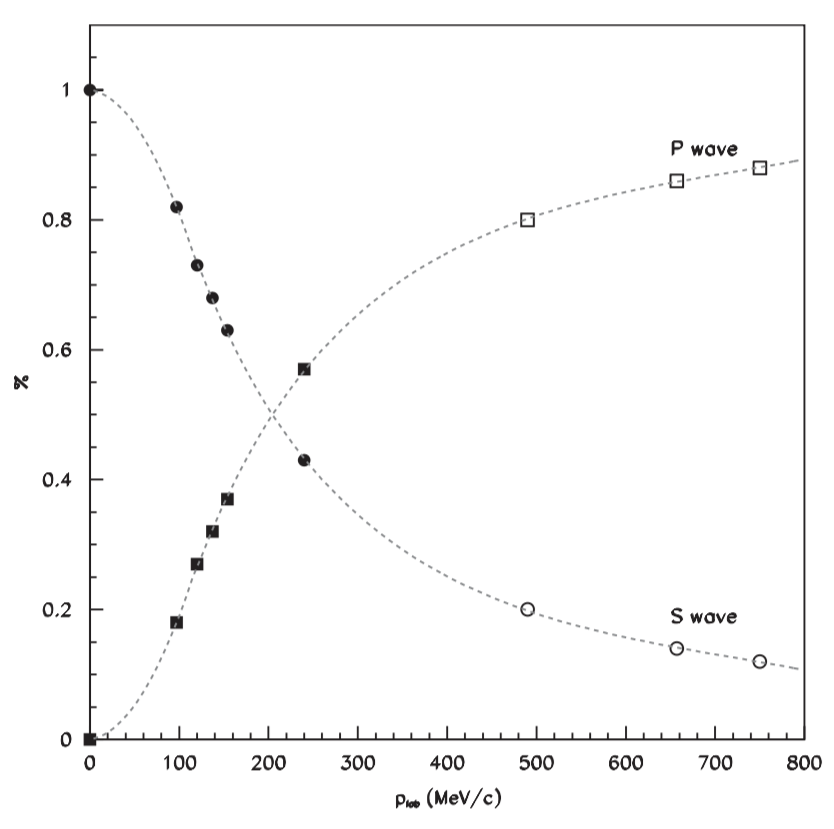
\includegraphics[width=0.70\textwidth]{nbar_exp/images/DoverRichard}
    \caption{Trends of S- and P-wave annihilation cross sections according to annihilation models: the full markers (circles for S-wave, squares for P-wave) are from the Dover–Richard model, while the open ones have been obtained by using a version of the optical model.}
    \label{fig:DoverRichard}
\end{figure}
Therefore, the $\bar{n}p$ system can be represented as an isospin eigenstate $|I, I_3\rangle = |1, +1\rangle$. It is not a C-parity eigenstate, then only J (total angular momentum), P (spatial parity) and G-parity are good quantum numbers, where G-parity is defined as the combination of charge conjugation and a rotation of $180^\circ$ in isospin space as $G = C\,e^{i\pi I_2}$.
$\\$
Since $\bar{n}p$ is an antifermion-fermion system, the following equations can be obtained:
\begin{center}
$P = (-1)^{L+1}$ \hspace{0.3cm} $G = (-1)^{L+S+1}$ 
\end{center}
where L is the relative angular momentum between the anti-neutron and the proton, while S is the spin of the system, namely 0 or 1. The $I^G(J^P)$ quantum numbers allowed for the lowest initial states are shown in Tab.~\ref{tab:q_number}.
\begin{table}[h]
  \centering
  \begin{tabular}{llll}
    \hline
    Wave & ${}^{2S+1}L_J$ & $I^G(J^P)$ \\
    \hline
    % S-wave
    S & ${}^{1}S_{0}$ & $1^{-}(0^{-})$ \\
      & ${}^{3}S_{1}$ & $1^{+}(1^{-})$ \\
    \hline
    % P-wave
    P & ${}^{1}P_{1}$ & $1^{+}(1^{+})$ \\
      & ${}^{3}P_{0}$ & $1^{-}(0^{+})$ \\
      & ${}^{3}P_{1}$ & $1^{-}(1^{+})$ \\
      & ${}^{3}P_{2}$ & $1^{-}(2^{+})$ \\
    \hline
    % D-wave
    D & ${}^{1}D_{2}$ & $1^{-}(2^{-})$ \\
      & ${}^{3}D_{1}$ & $1^{+}(1^{-})$ \\
      & ${}^{3}D_{2}$ & $1^{+}(2^{-})$ \\
      & ${}^{3}D_{3}$ & $1^{+}(3^{-})$ \\
    \hline
  \end{tabular}
  \caption{Quantum numbers $I^G(J^P)$ on $S$, $P$ e $D$ waves.}
  \label{tab:q_number}
\end{table}
$\\$
Even if the total cross section $\sigma_T$ is the first piece of information on the interaction between to particles, for the case $\sigma_T(\bar{n}p)$ could be tough to measure it. The final value of $\sigma_T$ published in \cite{armstrong1987} shows how the data could be fitted to a simple parametrization \cite{bertin1997}, obtaining the results showed in Fig.~\ref{fig:cross_section}.
\begin{figure}[h]
    \centering
    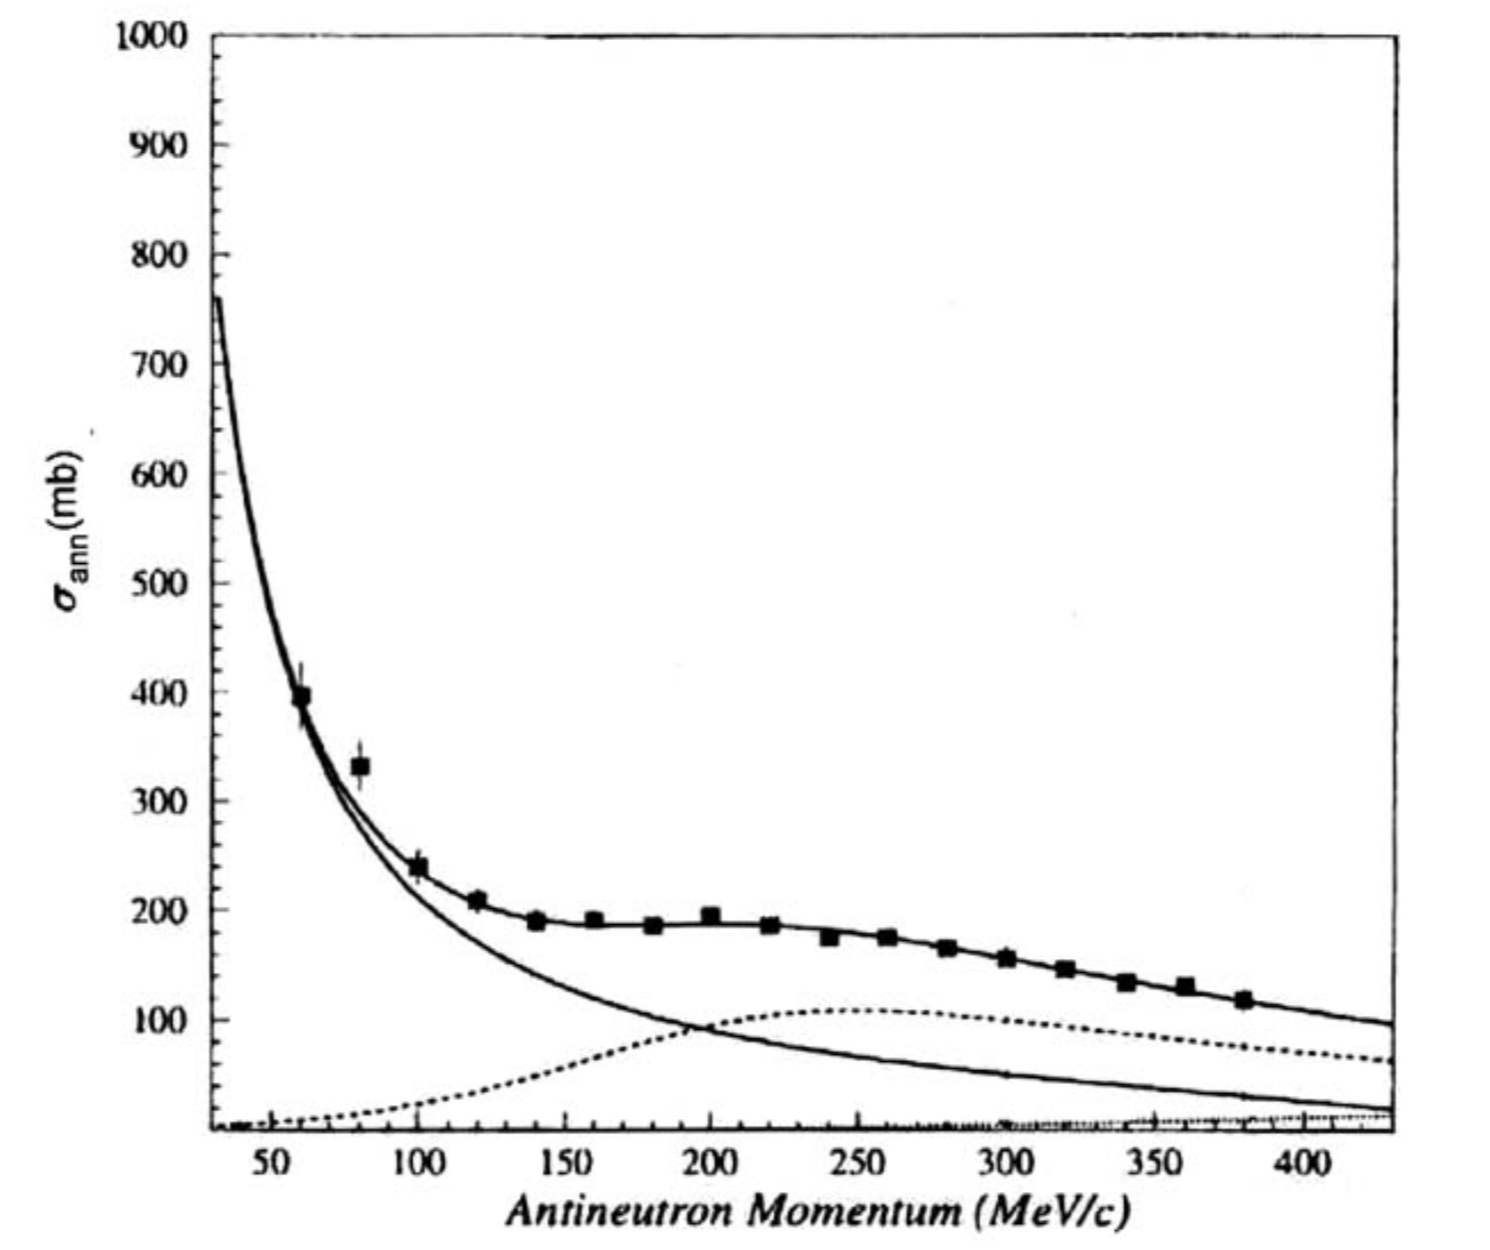
\includegraphics[width=0.55\textwidth]{nbar_exp/images/cross_section}
    \caption{Fit of the annihilation cross section $\sigma_{ann}(\bar{n}p)$, measured by OBELIX up to 400 MeV/c, including S (solid line), P (dashed line) and D (dotted line) wave contribution.}
    \label{fig:cross_section}
\end{figure}

\subsubsection{The anti-nucleon–nucleon interaction}
The first approach to describe the antinucleon-nucleon ($\bar{N}N$) interaction relies on interaction models. Unlike Quantum ElectroDynamics (QED), where the coupling constant $\alpha$ grows with energy and diverges at finite energy, asymptotic freedom characterizes the  Quantum ChromoDynamics (QCD), the quantum field theory of the strong force between quarks and gluons. Quarks interact weakly at high energies, enabling perturbative calculations, but at low energies the interaction strengthens dramatically, confining quarks and gluons within composite hadrons. Here, the divergent coupling constant $\alpha_s$ renders perturbative approaches invalid, making interaction models essential for describing strong interactions in the $\lesssim 1$ GeV energy range.
$\\$
The core of this approach is that, following the $\bar{N}N$ annihilation, a \emph{fireball} (which represents the $\bar{N}N$ system) with definite energy and volume $\Omega = \frac{4}{3}\pi R_0^3$ is formed, where $R_0 \sim 1$ fm is the nucleon radius. All the possible $\bar{N}N$ annihilation final states -primarily light mesons- may be reached through the decay of the fireball, according to the statistical Fermi model, where the probability of a final state is determined solely by the available phase space \cite{fermi1950}.
$\\$
The use of interaction models in $\bar{N}N$ interaction generally allows a correct description of annihilation, even if it doesn't reproduce the whole experimental scenario, such as differences between nucleon and anti-nucleon scattering and stopping power (Barkas effect) \cite{barkas1957}. The reason why it happens is the that the potential formulation used to describe the short range interactions (where annihilation plays the most important role) is not sensitive to the details of the internal dynamics, namely the interactions between quarks and gluons.
$\\$
The second approach is the Effective Range (ER) expansion one, which is independent on any hypothesis concerning the interaction potential and it is based on the obtained fit of experimental cross sections \cite{mahalanabis1988}. The annihilation cross section for two interacting particles may be expressed as a partial waves expansion as follows:
\begin{center}
$\sigma_{\text{ann}} = \sum_{L} \sigma^{\text{ann}}_{L} = \frac{4\pi}{k^{2}} \sum_{L} (2L + 1)\left(\Im m f_{L} - |f_{L}|^{2}\right)$,
\end{center}
where $k$ is the center-of-mass momentum of the incident particle, and the partial amplitude $f_L$ may be written as a function of the $\delta_L$ wave phase shifts induced by the interaction in the system wave function:
\begin{center}
$f_L = \frac{1}{cot\delta_L - i}$,
\end{center}

The partial waves may be expanded as a series in $k$, following the so-called \emph{Effective Range (ER) expansion formalism}:
\begin{center}
$k^{2L+1} \cdot cot\delta_L = \frac{1}{A} + \rho k^2 + O(k^4)$,
\end{center}
where A is the scattering length, and $\rho$ is the interaction range. For S and P partial waves can be obtained:
\begin{center}
$k \cdot cot\delta_0 = \frac{1}{a} + \frac{1}{2} r k^2$ \\
\vspace{0.3cm}
$k^3 \cdot cot\delta_1 = \frac{1}{b} - \frac{3}{2} \frac{1}{R} k^2$
\end{center}
$a$ and $b$ are, respectively, the scattering length and the nucleon volume, while $r$ and $R$ are the two effective ranges for the two partial waves. These parameters must be determined by a phenomenological fit to the annihilation cross section data. For example, for the $I=1$ case, relevant to the $\bar{n}p$ interaction case, it was found that \cite{bertin1997}:
\begin{center}
$a_1 = (0.4 + 0.5 i)$ fm and $r_1 = (-1.4 + 1.8 i)$ fm for S-wave, \\
\vspace{0.3cm}
$b_1 = (0.8 + 0.1i)$ fm$^3$ and $R_1 = (0.2 - 0.4 i)$ fm for P-wave
\end{center}

\subsubsection{Electromagnetic and hadronic showers}
In the energy scenario beyond 10 MeV, bremsstrahlung and pair production are the main processes which respectively involve electrons/positrons and photons, leading to the development of electromagnetic showers within the material. Therefore, to detect such phenomena, HEP experiments employ electromagnetic calorimeters. The electromagnetic calorimeter is a device whose size and density are designed to fully contain the electromagnetic shower, producing a signal proportional -or at least correlated- to the energy of the incident particle that initiated the shower. Since the radiation length $X_0$ (defined as the distance over which a high-energy electron loses $1/e$ of its energy through bremsstrahlung) determines the size of the electromagnetic shower, the typical longitudinal size for these detectors is of the order of 10-20 $X_0$ ($\sim 20-40$cm).
$\\$
Furthermore, hadronic showers can be originated from strong interactions of high energy (beyond $\sim GeV$) hadrons, such as protons, neutrons and pions, with the material. To detect this kind of showers, a hadronic calorimeter may be employed; since the interaction length $\lambda$ determines the hadronic shower size and $\lambda >> X_0$, hadronic showers are larger and longer than electromagnetic ones, requiring hadronic calorimeters to be significantly bigger than electromagnetic calorimeters. Therefore, homogeneous calorimeters cannot be used for hadronic calorimetry as they are for electromagnetic calorimetry. Instead, the sampling calorimeter technique is mandatory, employing alternating layers of passive, dense absorber material and active detection material.
$\\$
For example, approximately 95\% of a hadronic shower is contained within a cylinder of radius equal to the hadronic interaction length ($\lambda_{had} \simeq 44.1$ cm, in CsI(Tl)). In contrast, about 90\% of an electromagnetic shower is contained within a cylinder defined by the Molière radius ($R_M \simeq 3.6$ cm in CsI(Tl)). Therefore, there is an order of magnitude difference between the two values. A shape comparison between these two type of shower can be observed in Fig.~\ref{fig:shower_comp}.

\begin{figure}[H]
    \centering
    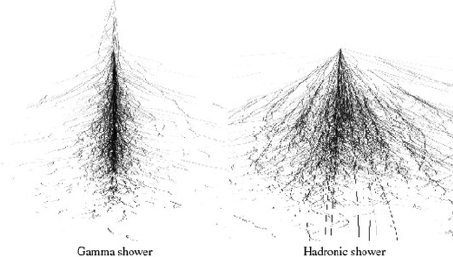
\includegraphics[width=0.60\textwidth]{nbar_exp/images/gamma_vs_hadronic}
    \caption{Electromagnetic shower vs hadronic shower comparison.}
    \label{fig:shower_comp}
\end{figure}

The $\bar{n}$ primarily interacts via the strong nuclear force, annihilating with nucleons in the material ($\sigma \sim 100$ mb), mainly producing light mesons such as pions which subsequently interact within the calorimeter:
	\begin{center}
		$\bar{n} + p/n \rightarrow \pi^{\pm}, \pi^0 ..$
	\end{center}
	
The $\pi^0$ meson mainly ($\sim 98.8 \%$) decays into a couple $\gamma \gamma$, producing electromagnetic showers that are fully contained in the calorimeter.
$\\$
While charged pions $\pi^+$ and $\pi^-$ undergo both electromagnetic and hadronic interactions, producing final products that are not fully contained within the calorimeter volume, this leads to a lack in the energy deposited in the detector. Both forward and backward directions are then involved, according to the reaction kinematics.

\subsection{The MANTRA Project}
It may be challenging for general-purpose experiments to directly identify and reconstruct anti-neutrons produced in $e^+e^-$ collisions, such as those at Belle II and BESIII, which lack a hadronic calorimeter. Anti-neutrons generally annihilate with detector material nucleons such as that of an electromagnetic calorimeter, producing hadronic showers which only allows a loose measurement of the anti-neutron energy with extremely large uncertainty.
$\\$
Since anti-neutron kinematics have so far been measured via missing mass methods or isospin symmetry with anti-protons, a direct anti-neutron reconstruction would be highly  desirable, especially in studying processes with neutral hadrons, such as $B^+ \rightarrow K^+ n \bar{n}$ or $J/\Psi \rightarrow p \pi^- \bar{n}$.
$\\$
This thesis fits in the larger context of the MANTRA (Measuring Anti-Neutron: Tagging and Reconstruction Algorithm) PRIN2022 project, an inter-university (University of Turin and University of Ferrara) and INFN effort aimed at developing a method to improve the reconstruction of anti-neutron in existing high-energy physics experiments. It provides a general approach to measure the energy of anti-neutrons $\bar{n}$ up to 10~GeV using an electromagnetic calorimeter. The main idea is to combine the information from a high time-resolution time of flight detector (TOP and TOF in the Belle II and in the BESIII experiments, respectively) with that from an electromagnetic calorimeter (ECL and EMC in the Belle II and in the BESIII experiments, respectively), where the anti-neutrons annihilation occurs.
$\\$
Due to its neutral charge and its immediate annihilation, tagging $\bar{n}$ can be very challenging. However, the annihilation can produce self-contained light mesons, mostly made of high-energy pions ($\pi^-, \pi^0, \pi^+$) and soft nuclear fragments. These can be detected in the Electromagnetic Calorimeter (detailed examination in the next chapter), where charged pions can produce hadronic showers, while neutral pions immediately decay into two photons which produce electromagnetic showers in the calorimeter volume. The comparison of the cluster energy deposition patterns, the so called shower shapes variables, left in the ECL by anti-neutrons and other neutral particles, such as photons, can improve the characterization of neutral particles.
$\\$
A crucial aspect of the analysis process is the role of simulation, where GEANT4 \cite{geant4_cds} (more details in the next chapter) plays a central role, modeling the hadronic interactions in the calorimeter; realistic simulation is essential to accurately reproduce real data. For $\bar{n}$ annihilation, parameterizations are typically derived from $\bar{p}$ measurements, necessitating validation against data.
$\\$
This thesis aims to study the $\bar{n}$ hadronic interactions modeled by simulation software and compare them with those observed in Belle II data, focusing exclusively on signals from the Belle II electromagnetic calorimeter. To achieve this, $\bar{n}$ variables are first studied using a signal sample, where only the specifically selected processes with $\bar{n}$ in the final state are generated. Several background channels are then included to simulate the complete Belle II environment, concluding with a comparison between the results obtained from simulations and those from real data, with a Data/MC agreement.
$\\$
Therefore, this work addresses the following question:

\begin{center}
\textbf{Are $\bar{n}$ hadronic showers correctly simulated in the Belle II software?}
\end{center}

\clearpage
\section{The Belle II experiment}
The following sections introduce the \textbf{SuperKEKB} \cite{akai2018} collider, describing its technical setup briefly. It then presents the \textbf{Belle II} \cite{BelleIIPhysicsBook2019} detector discussing it sub-detector by sub-detector. Afterwards, the Belle II Analysis Software Framework (\textbf{basf2}) and \textbf{TopoAna} program are briefly described, with attention to the role of Monte Carlo methods in collider experiment simulation and reconstruction.

\subsection{The SuperKEKB collider}
\textbf{SuperKEKB} \cite{akai2018} is an asymmetric $e^+ e^-$ double-ring collider, located at KEK (The High Energy Accelerator Research Organization), in Tsukuba, Japan. It is the upgrade of the previous collider KEKB. It has a circumference of $3016$ m and collides bunches of electrons with bunches of positrons, respectively of energy 7 GeV (High Energy Ring -HER-) and 4 GeV (Low Energy Ring -LER-). Figure ~\ref{fig:superkekb_scheme} is a schematic image of the SuperKEKB design:

\begin{figure}[h]
    \centering
    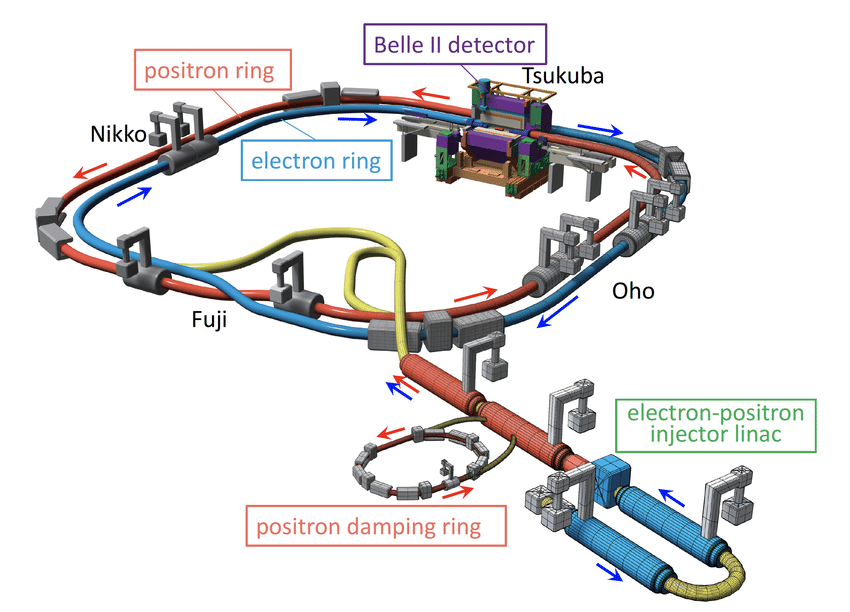
\includegraphics[width=1\textwidth]{belleII_det/images/superkekb.png}
    \caption{SuperKEKB design, where the Interaction Point (IP) is located in Tsukuba surrounded by the Belle II detector.}
    \label{fig:superkekb_scheme}
\end{figure}
It is noteworthy that the positron damping ring reduces the $e^+$ beam emittance, as positrons are obtained from a rotating tungsten target subjected. Electrons, by contrast, are injected directly from the linac since a controlled $e^-$ beam can easily be obtained \cite{kikuchi2005}.
$\\$
The resulting center-of-mass enrgy $\sqrt{s}$ in the IP can be modulated, but most of the data are acquired at the $\Upsilon(4S)$ resonance (10.58 GeV), an excited quarkonium state of $b \bar{b}$, which mainly decays into an entangled couple of $B\bar{B}$ ($\sim 100\%$). The $\Upsilon(4S)$ mass is just 20 MeV above the $B\bar{B}$ threshold, then the mesons are produced nearly in the rest frame. Since the lifetime of neutral B-mesons is short ($\tau = 1.510$ ps) and they are produced with low velocities, their path before decaying is short, making tough to separate the decays of the two produced mesons. The explicit asymmetry of bunches results in a relativistic forward Lorentz boost of the center-of-mass, where the decay length of the mesons is longer in the LAB frame, allowing the observation of the B mesons. Due to the huge amount of produced B mesons, SuperKEKB is regarded as an example of so-called (super) \textbf{B-factory}. 
$\\$
SuperKEKB has been running since 2018 and it achieved the world’s highest instantaneous luminosity ($5.244 \times 10^{34} cm^{-2} s^{-1}$ ) in March 19, 2026. The design luminosity of SuperKEKB  $ 8 \times 10^{35} cm^{-2} s^{-1}$, 40 times higher than Belle's one, with the goal to accumulate data corresponding to an integrated luminosity of 50 $ab^{-1}$. The SuperKEKB 24-Hour Operation Summary is shown in figure ~\ref{fig:SuperKEKB 24-Hour Operation Summary}.

\begin{figure}[h]
    \centering
    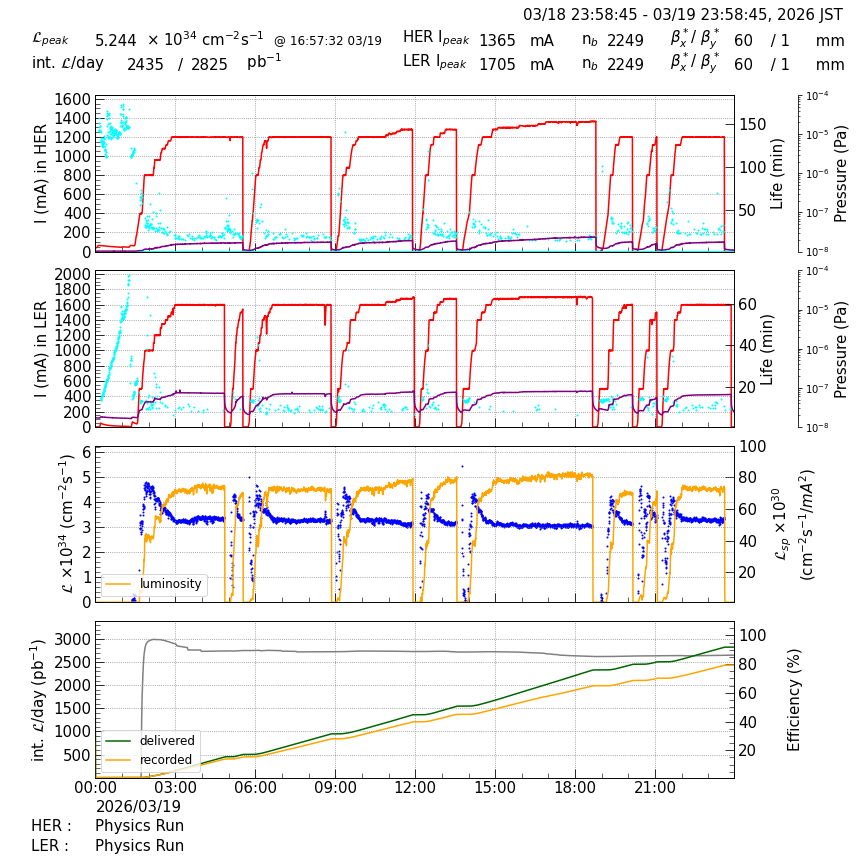
\includegraphics[width=0.8\textwidth]{belleII_det/images/SuperKEKB_operation.png}
\caption{SuperKEKB operating parameters on March 18-19, 2026. From top to bottom: HER and LER ring currents (first two panels), instantaneous and integrated luminosity (bottom two panels)}
\label{fig:SuperKEKB 24-Hour Operation Summary}
\end{figure}

\subsection{The Belle II detector}
The only interaction point of SuperKEKB is surrounded by the \textbf{Belle II} detector \cite{BelleIIPhysicsBook2019}, a general purpose high-energy particle layered detector with almost $4 \pi$ of solid angle coverage. It presents a cylindrical shape to cover the $e^+ e^-$ collisions, composed of a barrel and two end-caps located along the z-axis. 
$\\$
The Belle II detector measures 8 m in both width and height, with a total weight of approximately 1400 tons. With the exception of the KLM, all its subsystems are immersed in a 1.5 T magnetic field. 
$\\$
The detector is composed of several sub-detectors arranged cylindrically, reflecting the asymmetric distribution of the final state particles. The cylindrical structure of the detector is the \emph{barrel}, while the bases are made of the forward end-cap (along the direction of the $e^-$ beam) and the backward end-cap (along the direction of the $e^+$ beam). 
$\\$
The Belle II detector consists of the following sub-detectors, arranged radially outward from the IP:
\begin{enumerate}[label=(\alph*)]
\item Beam Pipe made of Beryllium (Be),
\item Two layers of silicon pixel detector (PXD),
\item Four layers of silicon strip detector (SVD),
\item The Central Drift Chamber for tracking the charged particle CDC, 
\item Time of propagation (TOP) Cherenkov counter in the barrel  + Cherenkov ring imaging (ARICH) in the front end-cap region,
\item The electromagnetic calorimeter (ECL) to detect photons and to identify charged particles, 
\item Superconductive magnet which provides 1.5 T axial magnetic field in order to bend charged particle, 
\item $K_L$ and muon detector (KLM) to track muons and $K_L$. 
\end{enumerate}

The electromagnetic calorimeter (ECL) has a central role in this elaborate since neutral ECL clusters associated to anti-neutron candidates are studied.
$\\$
A Belle II scheme is shown in ~\ref{fig:belleii_artistic}.

\begin{figure}[H]
    \centering
    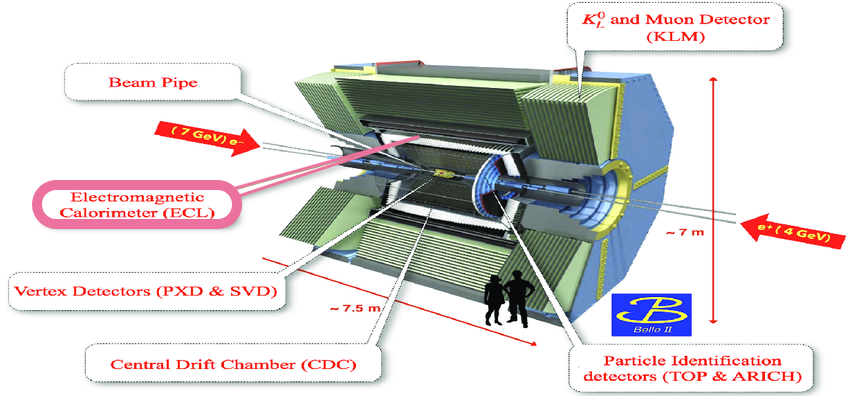
\includegraphics[width=1\textwidth]{belleII_det/images/belleii_dets}
    \caption{An artistic view of the Belle II detector}
    \label{fig:belleii_artistic}
\end{figure}

\subsubsection{The vertex detector VXD}
Immediately following the beryllium beam pipe, which does not play a detection role, the innermost layer is the Vertex Detector (\textbf{VXD}). 
$\\$
It consists of two devices: the Silicon Pixel Detector (\textbf{PXD} - 2 layers) \cite{YE2021164875} and the Silicon Vertex Detector (\textbf{SVD} - 4 layers) \cite{ZANI2022166952} . Overall there are six layers, of whose the first two ($r_1=14 mm, \ r_2=22 mm$) are pixelated sensors of the DEPFET type and the remaining four ($r_3=38 mm, \ r_4=88 mm, \ r_5=115 mm,\ r_6=140 mm$) are double-sided silicon strip sensors. 
$\\$
The VXD provides coverage of $17^\circ < \theta < 150^\circ$ and full azimuthal coverage in $\phi$, where $\theta$ is the polar angle relative to the $z$-axis -aligned with the $e^-$ beam direction- and $\phi$ is the azimuthal angle in the $xy$ plane using cylindrical coordinates.

\begin{figure}[H]
    \centering
    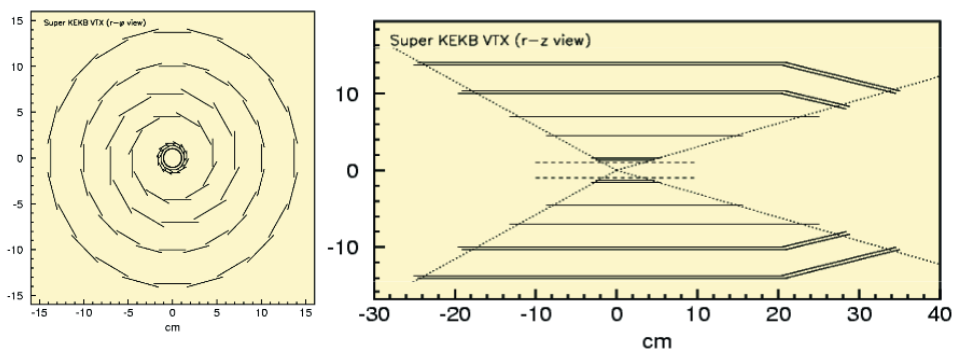
\includegraphics[width=0.95\textwidth]{belleII_det/images/VXD}
    \caption{A scheme of the Belle II VXD}
\end{figure}

The VXD purpose is to reconstruct the position of the primary vertex, the vertex of B-mesons decay which are directly produced by the decay of the $\Upsilon(4S)$, improving the resolution of the tracking system as well..

\subsubsection{The Central Drift Chamber (CDC)}
The Central Drift Chamber (\textbf{CDC}) is a large volume composed of small drift cells and it is the main tracking system of the Belle II detector, reconstructing charged-particle tracks by measuring the hit positions, which allows the determination of their momenta \cite{Taniguchi_2017}. Furthermore, the energy loss $\frac{dE}{dx}$ measure provides information for PID (Particle IDentification), thanks to the 1.5 T magnetic field. CDC has a radius of 1130 mm and it contains 14339 wires in total distributed in 56 layers, either parallel (axial orientation) or skewed (stereo orientation) to the longitudinal magnetic field . Combining their information, it is possible to reconstruct a full tridimensional helix track. Inside the cell, the average drift velocity is $3.3 \frac{cm}{\mu s}$. 
$\\$
The CDC has the same VXD angular ($\theta$, $\phi$) coverage and, in order to increase the forward acceptance, it is distributed asymmetrically along the z axis. It is filled with a mixture of $H_e C_2 \ (50\%)$ and $H_6 \ (50\%)$, which represents a good trade-off between a good momentum resolution for tracking and good $\frac{dE}{dx}$ resolution for the PID. A schematic view of the CDC is shown below:
\begin{figure}[H]
    \centering
    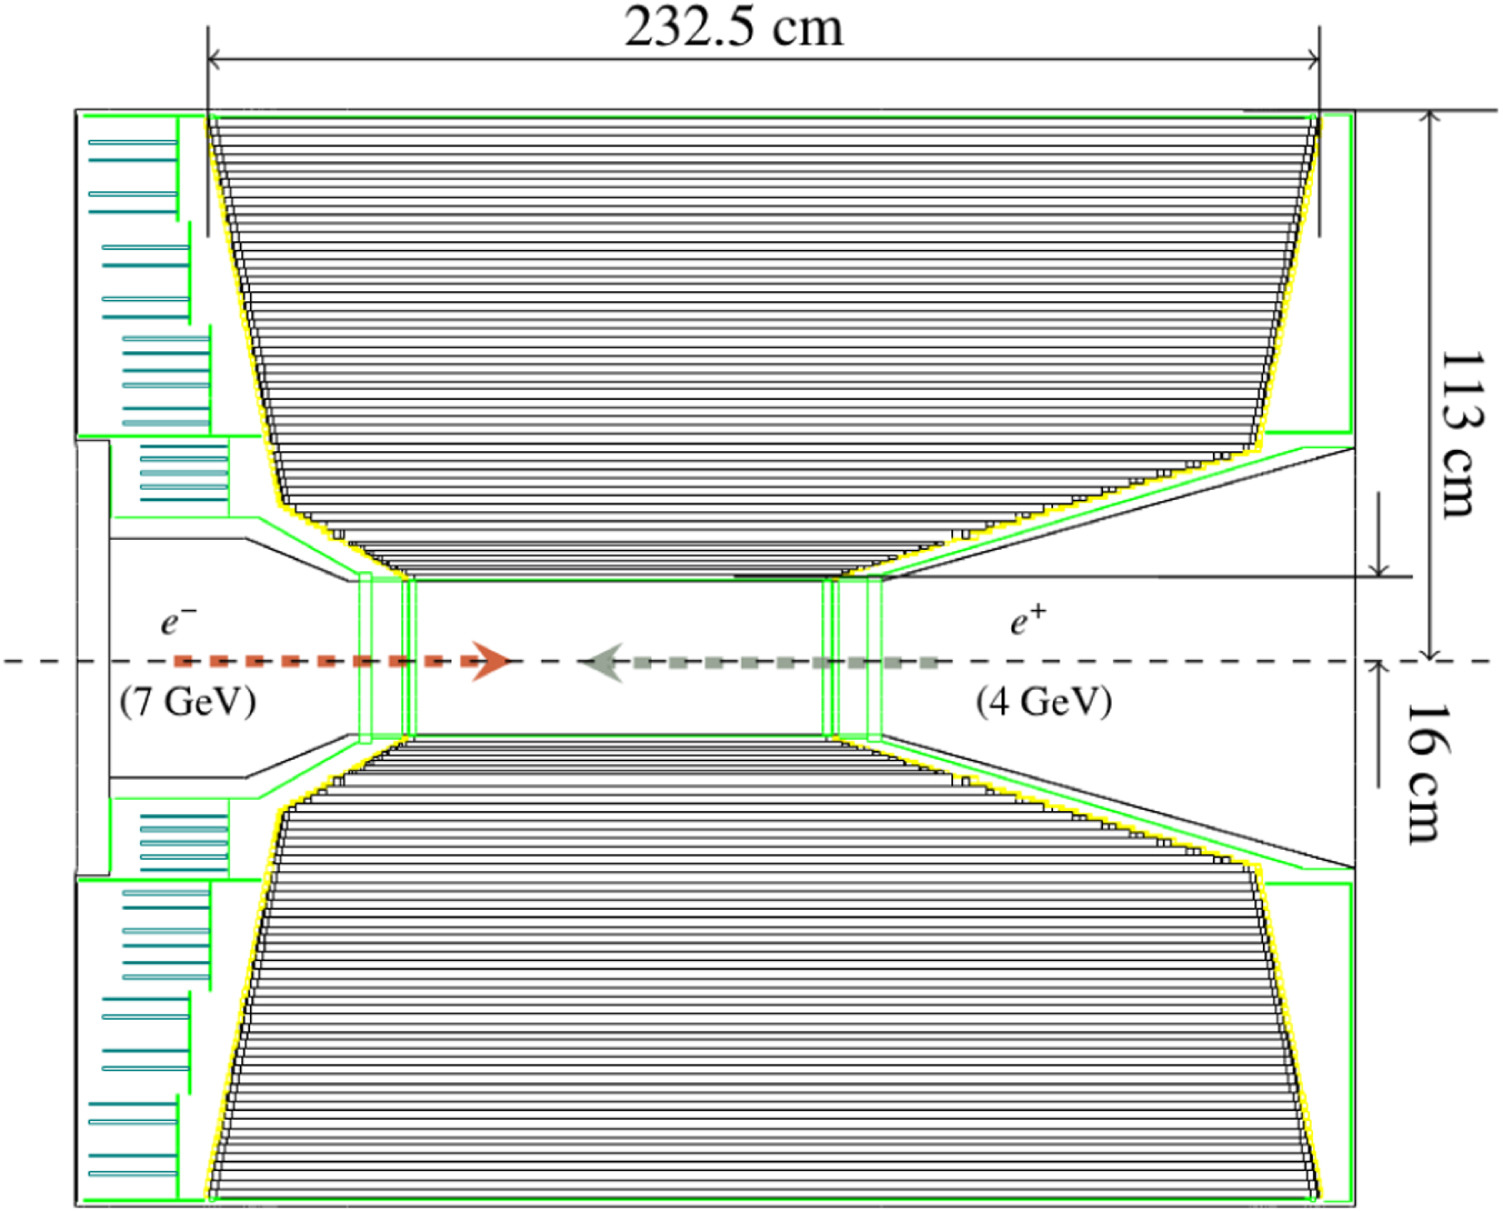
\includegraphics[width=1\textwidth]{belleII_det/images/CDC}
    \caption{A scheme of the Belle II CDC}
\end{figure}

\subsubsection{PID system: TOP and ARICH}
Particles crossing a Cherenkov radiator material with a speed $\beta > \frac{c}{n}$, where c is the speed of light and n is the material refractive indices, emit photons at an angle of $\theta_c = arcos(\frac{1}{\beta n})$.
$\\$
For Particle Identification in the barrel region, a Time of Propagation (\textbf{TOP}) counter is employed. It is a novel type of Cherenkov detector \cite{Horii:2013ndq} used for particle identification in the barrel region. In total, there are 16 modules, each consisting of a 45 cm wide and 2 cm thick quartz bar with a small expansion volume of about 10 cm long at the sensor end. There is an expansion wedge that behaves as a lens and improves the spatial resolution of the Cherenkov photon imaging. At the exit window of the wedge, two rows of sixteen fast multi-anode photon detectors are mounted.
$\\$
Within the 2.6 m-long quartz the particle produces Cherenkov radiation that travels via total internal reflection to the mirror, where they are reflected towards the photon detectors at the backward end, where is located a small prism which serves as a volume expansion and a light guide. The time of arrival and the impact position of the Cherenkov photons provide the 2D Cherenkov ring signal. 
$\\$
The hit distributions differ according to the particle species and their masses: different particles exhibit distinct Cherenkov angles, resulting in different photon paths. Consequently, they are detected at different positions within the PMT array and at different times.


\begin{figure}[h]
    \centering
    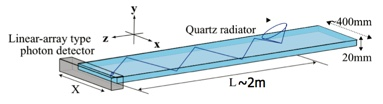
\includegraphics[width=0.8 \textwidth]{belleII_det/images/top}
    \caption{Scheme of TOP counter module}
\end{figure}

\begin{figure}[h]
    \centering
    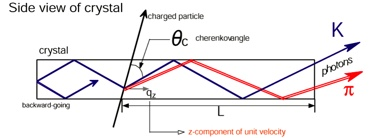
\includegraphics[width=0.8 \textwidth]{belleII_det/images/top2}
    \caption{Representation of the side view of TOP counter with internal reflection of the Cherenkov radiation}
\end{figure}

Thanks to a 16-channel Micro Channel Plate PhotoMultiplier (MCP-PMT), TOP counters are equipped with photosensors that provide a time resolution of about 100 ps.
$\\$
The Aerogel Ring Imaging CHerenkov (\textbf{ARICH}) \cite{Yusa:2013cao} is located in the forward end-cap region of the Belle II detector and is thus complementary to the aforementioned TOP. Its main goal is to separate kaons $K$ from pions $\pi$ across the full kinematic range of the experiment, from 0.5 to 4.0 $GeV/c$.
$\\$
Since particles with the same momentum but different mass radiate at different angles, it is designed to detect and distinguish forward-going charged particles. It consists of two 2 cm thick layers of aerogel ($n_{up} = 1.045, n_{down} = 1.055$), which increase the photon yield without degrading the Cherenkov angle resolution.

\begin{figure}[H]
    \centering
    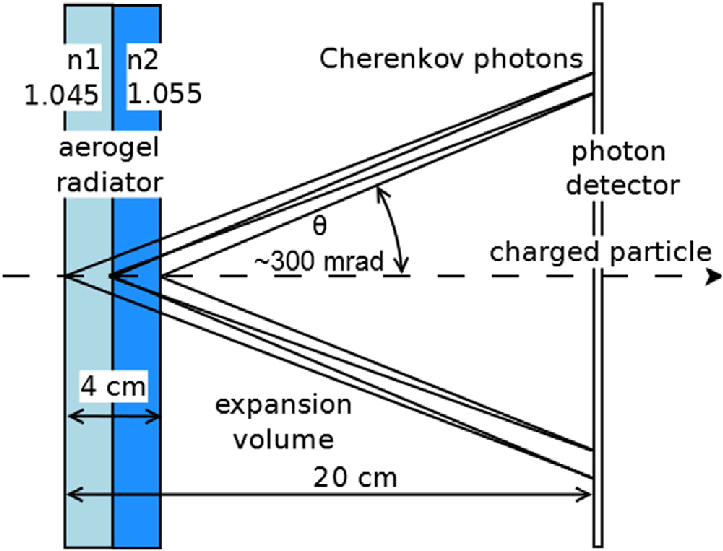
\includegraphics[width= 0.49\textwidth]{belleII_det/images/ARICH}
    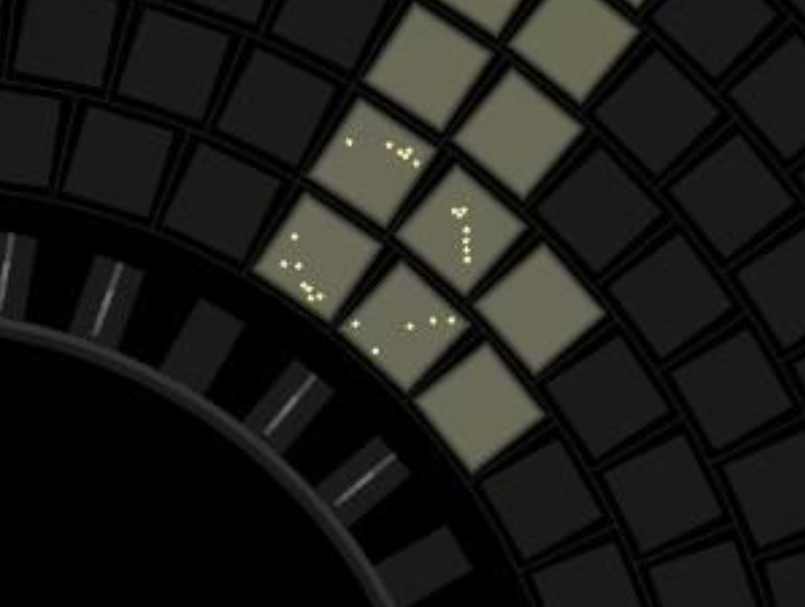
\includegraphics[width= 0.49\textwidth]{belleII_det/images/mu_ring}    
    \caption{(a) working principle of ARICH (b) ring produced by a cosmic muon}
    \label{fig:mesh2}
\end{figure}

\subsubsection{The Electromagnetic Calorimeter (ECL)}
The Electromagnetic CaLorimeter (\textbf{ECL}) plays a central role in this thesis, since the neutral ECL clusters associated to anti-neutron candidates are studied.
$\\$
A calorimeter is a detector designed to measure particle energy. As particles enter, they initiate electromagnetic or hadronic showers, depositing their energy within the detector material, which is then collected and precisely measured. 

\begin{figure}[h]
    \centering
    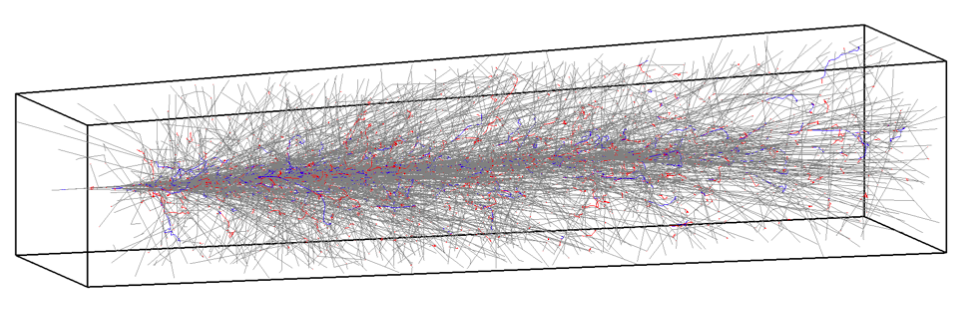
\includegraphics[width=0.95\textwidth]{belleII_det/images/shower_ECL}
    \caption{Typical ECL shower caused by a 7 GeV photon}
\end{figure}

However, as its name suggests, the primary aim of the ECL is to detect photons and electrons, providing precise measurements of the energy and position ($E$, $\vec{x}$) of electromagnetic showers \cite{KUZMIN2020162235}. It must identify neutral particles, such as photons and neutral hadrons, as well as charged ones (mostly electrons and pions). Anti-neutron is detected through its annihilation products (mainly pions), as previously discussed.
$\\$
The Molière radius $R_m$ is defined as 
\begin{center}
$R_m = \frac{21 MeV}{E_c} \times X_0$, where $E_c$ is the material critic energy
\end{center}
The rule of thumb for electromagnetic calorimeter is that $\sim 90\%$ of electromagnetic shower is contained in a cylinder with radius $R_m$, while the $\sim 95\%$ is contained in a cylinder with radius $2R_m$.

\paragraph{CsI(Tl) crystals}
$\\$
The thallium-doped caesium iodide \textbf{CsI(Tl)} crystals have $X_0$ = 1.860 cm and $R_m$ = 3.53 cm. This material is one of the brightest known scintillator, providing a light yield Y of  $\sim 52000$ photons/MeV, with a photon emission spectrum at $\sim 550$ nm, ideal for photodiode readout. 

\begin{figure}[H]
    \centering
    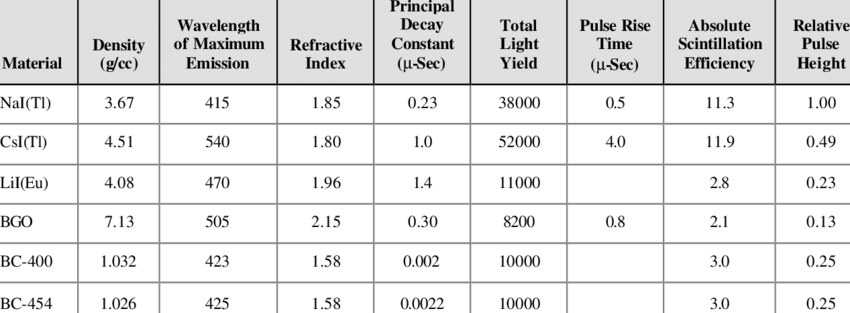
\includegraphics[width=1\textwidth]{belleII_det/images/Properties-of-scintillators}
    \caption{Properties of inorganic scintillators used in calorimetry \cite{nedilko2009}}
\end{figure}

The ECL is composed of 8736 array of \textbf{CsI(Tl)} crystals. Each is a truncated pyramid with dimension 6x6x30 $cm^3$, where the radial length is around 16.2$X_0$. Each crystals is wrapped with a layer of 200  $\mu m$ thick Gore-Tex porous teflon and then covered with a 50 $ \mu m$ thick aluminized polyethylene.
$\\$
The ECL is made of a 3 m long barrel section and the end-caps at $z = 2.0$ m (forward) and $z = -1.0$ m (backward). An ECL scheme is shown below:

\begin{figure}[H]
    \centering
    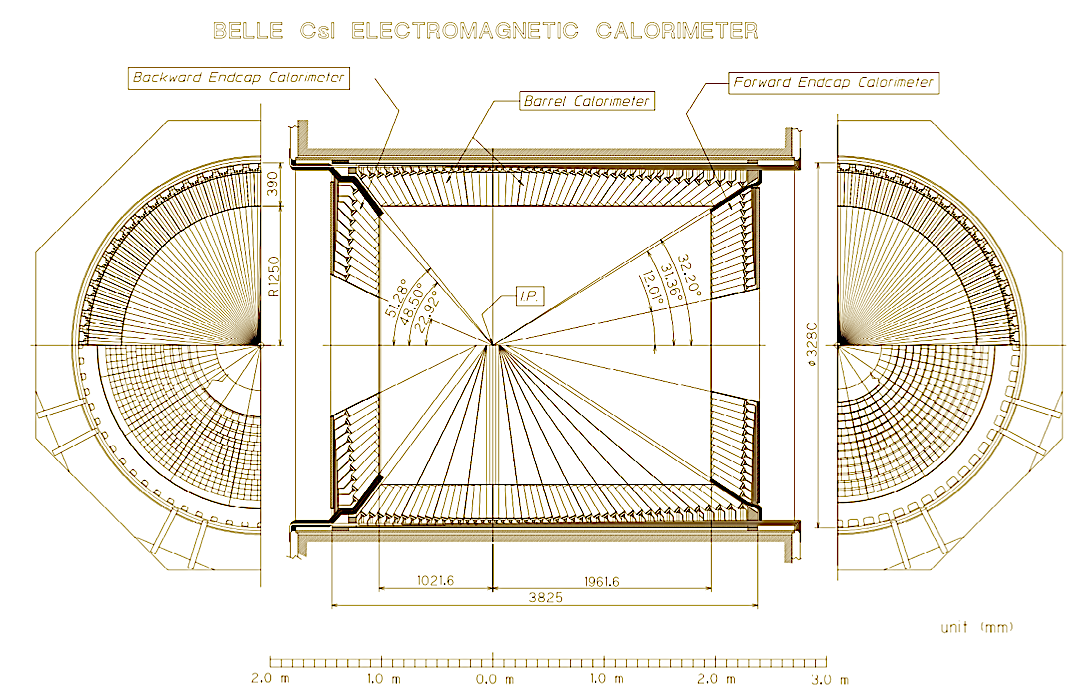
\includegraphics[width=1\textwidth]{belleII_det/images/ECL}
    \caption{A scheme of the Belle II ECL detector}
\end{figure}

It then is located in the barrel region and in the forward/backward end-cap region too, covering about 90\% of the solid angle in the center-of-mass system (polar coverage: $12^{\circ} \le \theta \le 155^{\circ}$); two $\sim1^{\circ}$ gaps between barrel and end-caps.
$\\$
Lights coming from each crystals is detected by two $10 \times 20 mm^2$ \emph{Hamamatsu S2744-08} photodiodes glued to the rear surface of the crystals and coupled with charge-sensitive pre-amplifiers.

\begin{figure}[H]
    \centering
    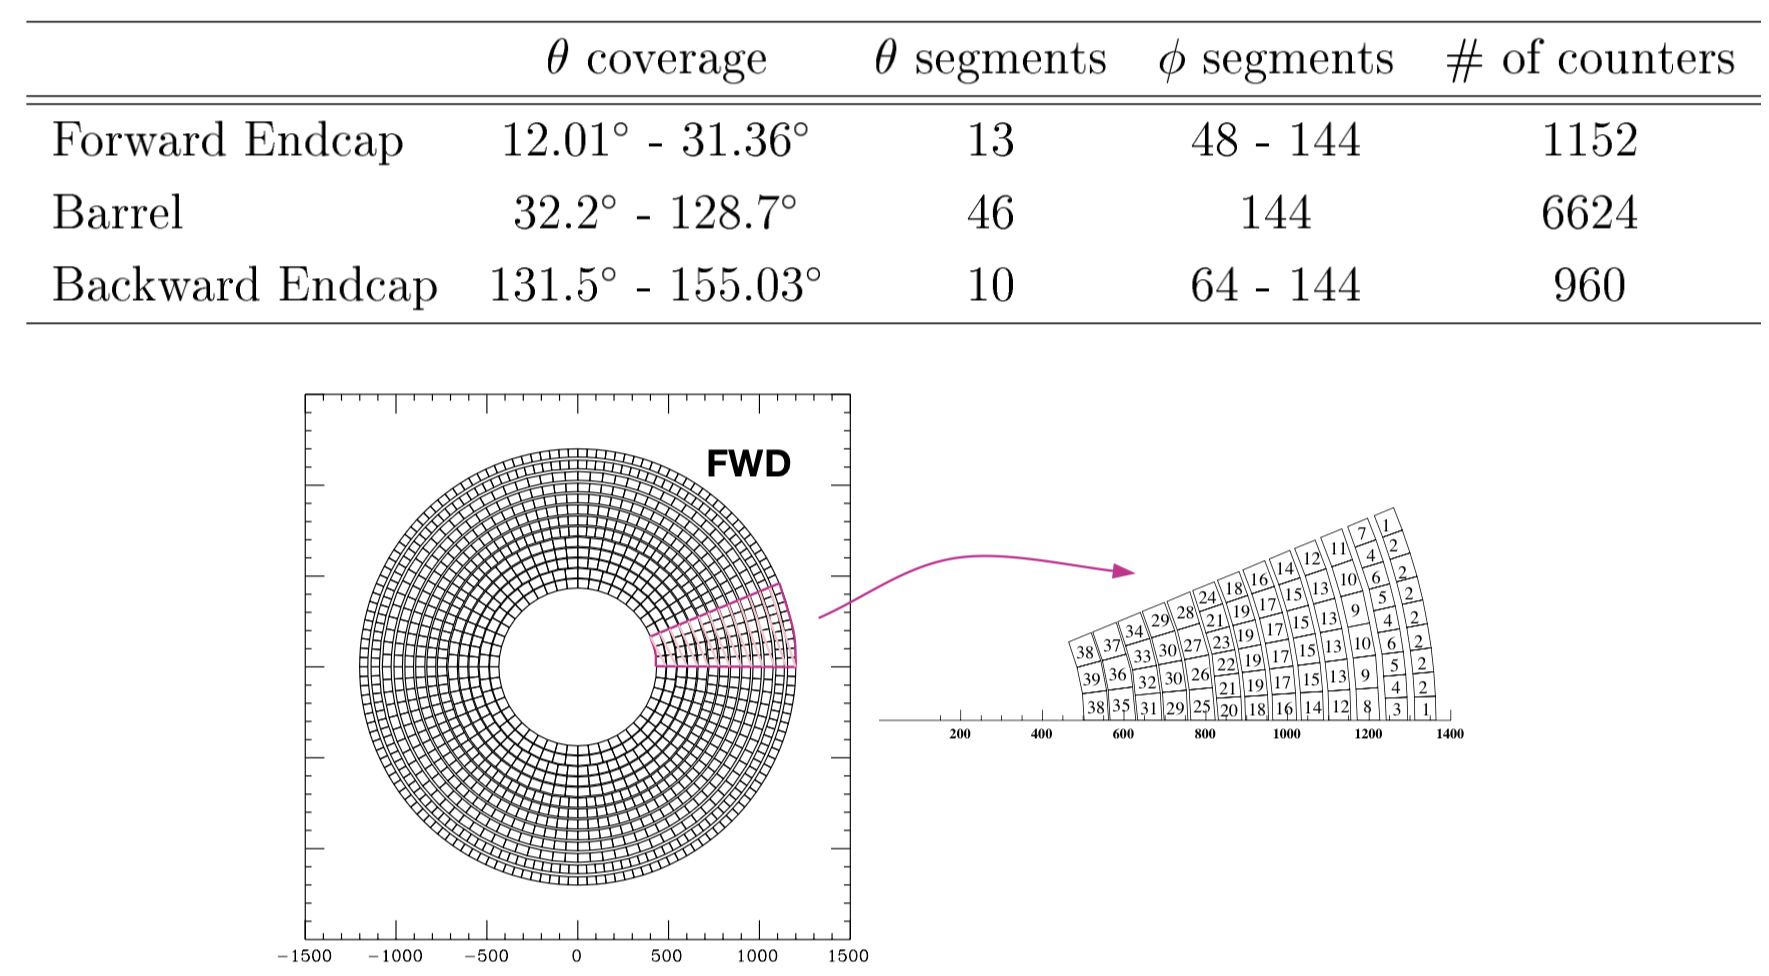
\includegraphics[width=0.85\textwidth]{belleII_det/images/ECL_division}
    \caption{ECL coverage and segmentation}
\end{figure}

\paragraph{The ECL  reconstruction algorithm} 
$\\$
as mentioned, the main tasks of an electromagnetic calorimeter are to measure the energy and position of electromagnetic showers and to identify neutral and charged particles. For each crystals, a 32 bit word is the result of the signal, namely an \textbf{ECLDigit}. It is made of the energy information in GeV (18 bit), the time information in ns (12 bit) and 2 status bits (quality of the signal). In order to reconstruct the shower, there is an algorithm which converts the ECLDigit into ECLShowers and the into ECLClusters.
$\\$
The first step is to identify the  \textbf{connected regions}, which allows a rapid reduction of the combinatorics. An example of this procedure is shown below:

\begin{figure}[H]
    \centering
    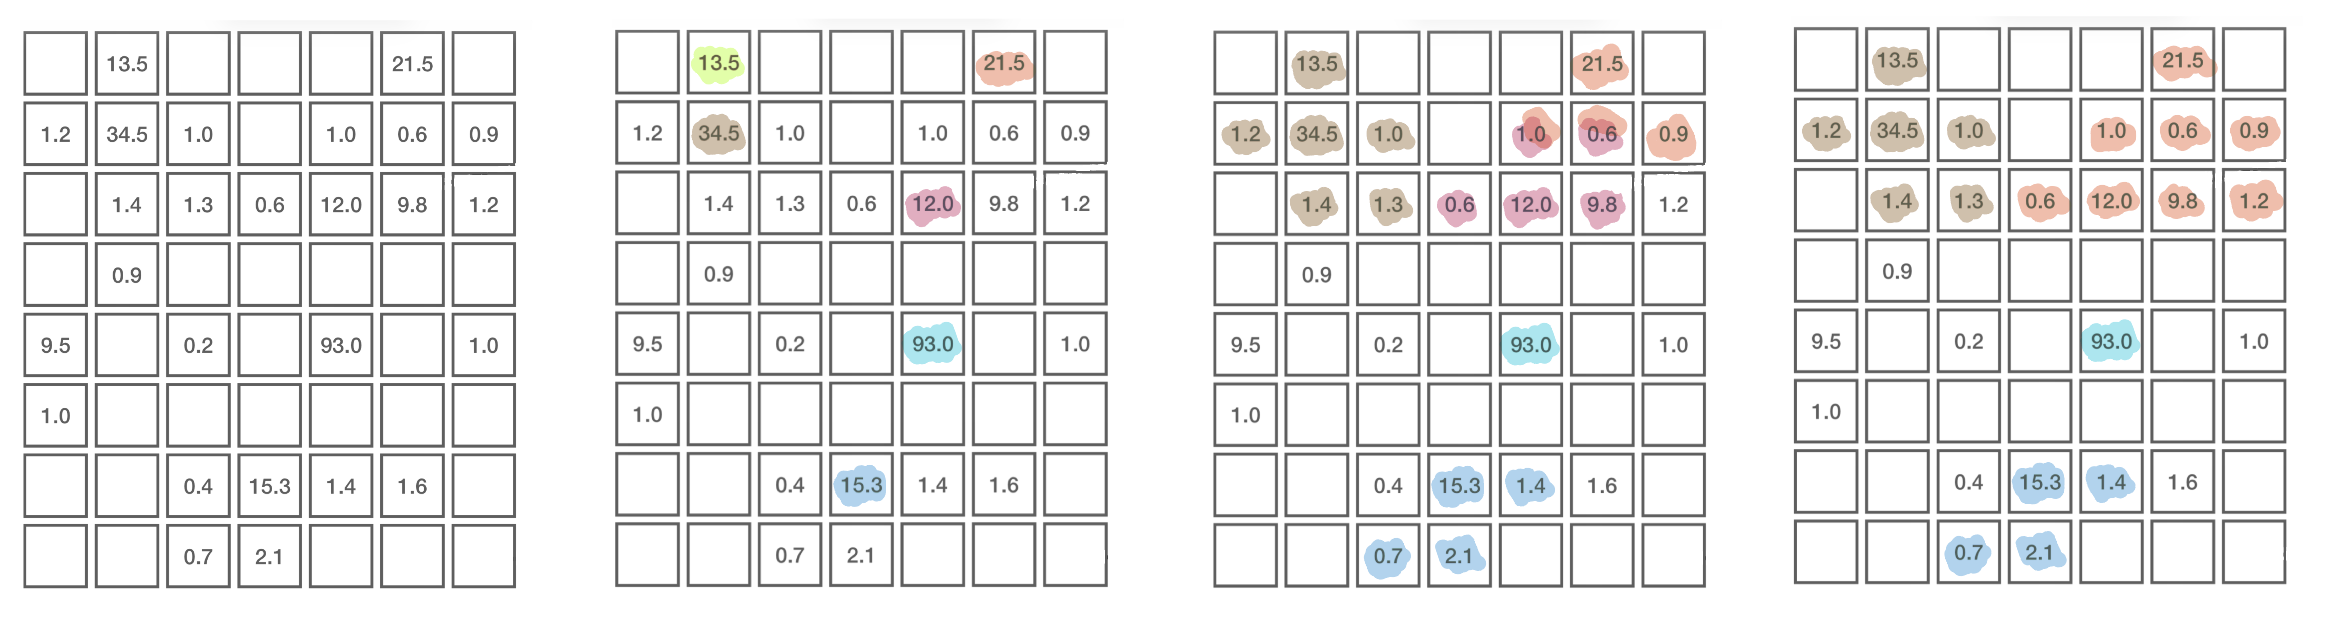
\includegraphics[width=1\textwidth]{belleII_det/images/ECL_algo}
  \caption{Description of ECL clustering process:(a) Step 0 (b) Step 1 (c) Step 2 (d) Step 3}
\end{figure}

Each cell represents one ECLDigit, whose value corresponds to the energy in MeV. Empty cells are below the readout threshold (0.1 MeV for this example). In step 1, every ECLDigit above 10 MeV is selected. In step 2, any neighbors above 0.5 MeV are attached to the highest-energy seed found in step 1. Sometimes two seeds compete for the same neighbor, and sometimes clusters have no neighbors (i.e. 93.0). In step 3, overlapping neighbor regions trigger a merge. Additionally, any cells above 1.5 MeV recruit their next neighbors iteratively.
$\\$
After this process, the connected regions are obtained:

\begin{figure}[H]
    \centering
    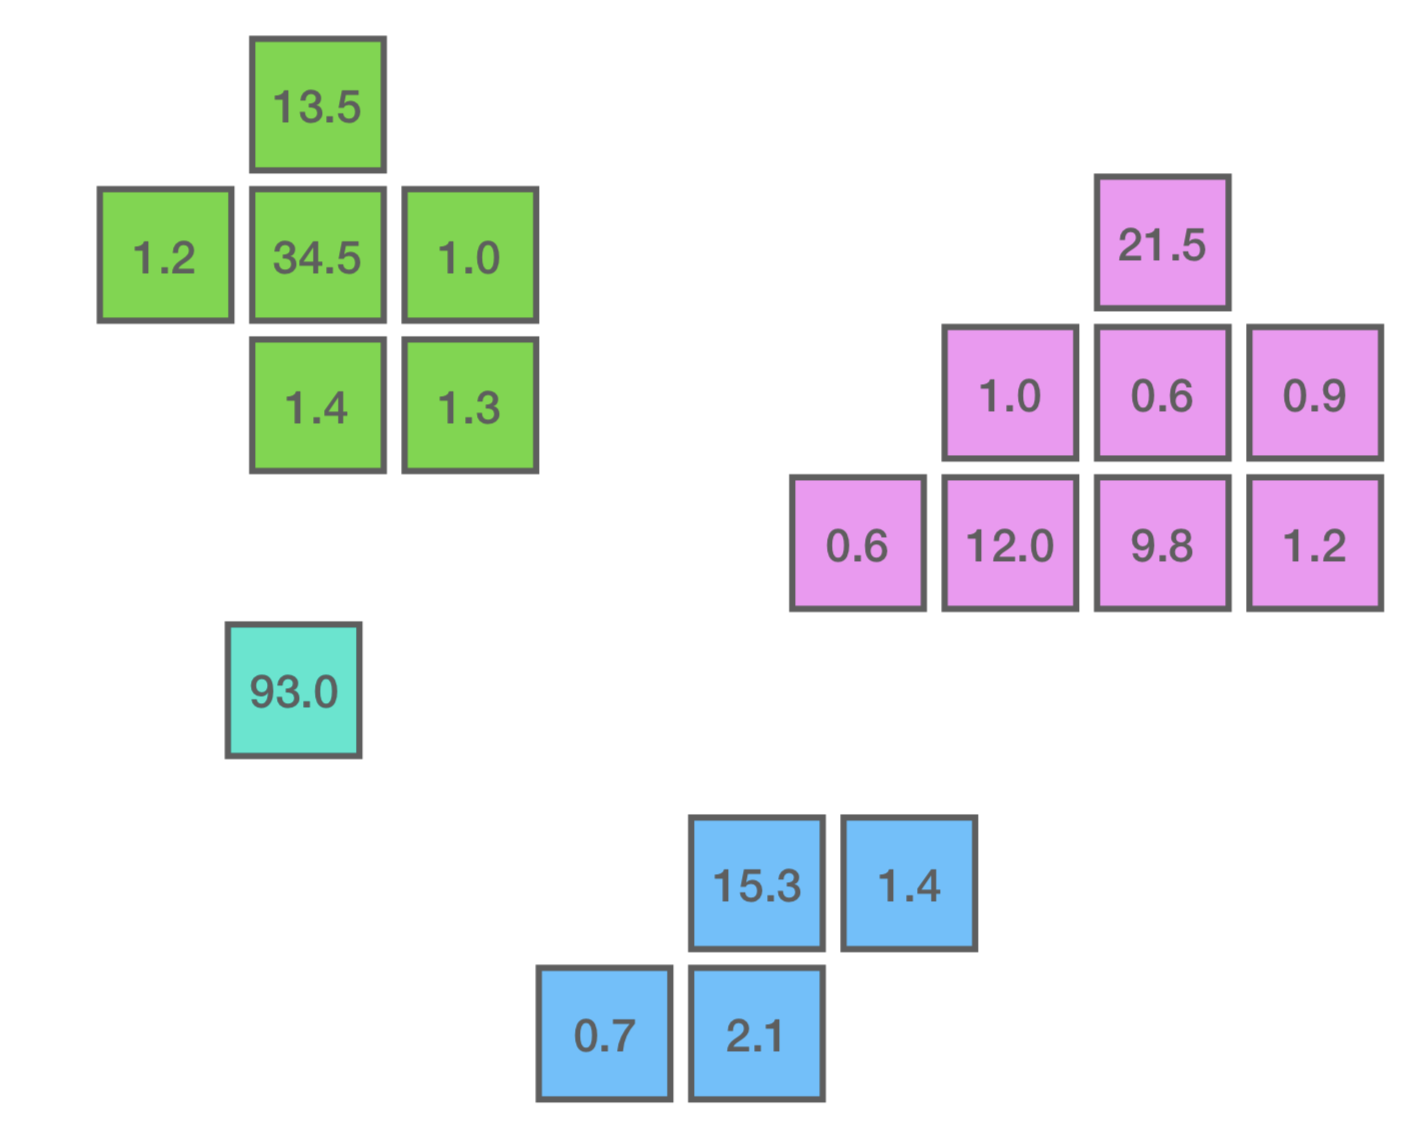
\includegraphics[width=0.5\textwidth]{belleII_det/images/ConnectedRegions}
\end{figure}
The final step is to pick the crystals with energy above 10 GeV, namely the Local Maxima (LM). Every connected region has one LM at least. The connected regions are furtherly processed in order to obtain the position and the energy of the cluster, processing the LM with a splitting-weighting process among the connected regions crystals \cite{denuccio2019}. 
$\\$
The main idea is that an \textbf{ECLShower} object is produced from every LM. If there is only one local maximum within a connected region, the full energy of each crystal is associated with the corresponding ECLShower. Otherwise, if multiple local maxima are present, an iterative procedure is performed, where the weight for each crystal depends on the distance of the crystal from the center-of-gravity of each ECLShower (enter-of-gravity is calculated using weighted energies).
$\\$
Connected regions are used to minimize the number of times the computationally intensive splitting procedure must be performed.

\paragraph{ECL performance}
$\\$
The observed ECL \textbf{energy resolution} can be written as follow:
\begin{center}
$\sigma_E = \sqrt{ \left( \frac{0.81\%}{\sqrt[4]{E}} \right)^2 + \left( \frac{0.066\%}{E} \right)^2 + (1.34\%)^2 }$
\end{center}
Where the first term represents stochastic fluctuations (Poissonian statistics) in shower generation, the second term accounts for electronic noise, and the third is a constant term dependent on calibration.
$\\$
For example, $\frac{\sigma_E}{E} = 4\%$ at 100 MeV and $\frac{\sigma_E}{E} = 1.4\%$ at 8 GeV, while the angular resolution is 13 mrad (3 mrad) at low (high) energies. For example, the $\pi^0$ mass is 135 MeV and its mass resolution is approximately 4.5 MeV, in absence of background (detailed description can be found in \cite{abashian2002}).

\begin{figure}[H]
    \centering
    \includegraphics[width=1\textwidth]{belleII_det/images/energy-res}    
\end{figure}

\begin{figure}[H]
    \includegraphics[width=1\textwidth]{belleII_det/images/energy-res2}
  \caption{The energy resolution as a function of incident photon energy for the (a) 3Y3 and (b) 5Y5 matrix with total energy sum. The energy resolution of the (c) 3Y3 and (d) 5Y5 matrix with a 0.5 MeV threshold. The solid lines are the results of the "t. The error bars are not statistical but are the rms of four measurements taken with the crystals (3,3), (3,4), (4,3) and (4,4) into the photon beam \cite{ikeda2000belle}}
\end{figure}


\subsubsection{Solenoid and iron structure} 
Following the ECL, an axial magnetic field of 1.5T is generated by a 23 tons superconducting solenoid. The curvature of charged-particle trajectories (Larmor radius) allows the determination of their momentum and charge, which, when combined with additional detector information, enables particle identification.
$\\$
It is made of niobium-titanium-copper (NbTi/Cu) alloy and it is cooled by liquid helium cryostat in order to reach superconducting conditions.
\subsubsection{The $K_L$ and Muon Detector (KLM)}
Following the solenoid, the \textbf{KLM} detector represents the outermost layer of Belle II and it is dedicated to the detection of $K_L$ mesons and muons, which are very penetrating particles. It is composed of alternating layers of 4.7 cm thick iron plates and active detector elements; the former acts as a return yoke for the magnetic flux. They also provide at least 3.9 interaction lengths (compared to 0.8 in the ECL), allowing the $K_L$ to interact and produce hadronic showers.
$\\$
KLM covers the barrel region (15 layers) and the end-caps regions (forward 14 layers and backward 12 layers). The two inner barrel layers and the entire end-caps are instrumented with scintillator strips, while the 13 outer barrel layers are instrumented with Resistive Plate Chambers (RPC). 
$\\$
As compared to charged hadrons, muons travel longer distances and with smaller deflections inside the KLM, which allows discrimination between the two.

\subsection{The Belle II Analysis Software Framework}
\begin{figure}[H]
    \centering
    
\includegraphics[width=0.4\textwidth]{belleII_det/images/b2logo}
\end{figure}

To perform the simulations, reconstruction and the analyses of this thesis, the Belle II Analysis Software Framework (\textbf{basf2}) has been employed. It is the primary software used in all aspects of the online data-processing chain at Belle II, such as generating simulated data, unpacking raw data, performing reconstruction (tracking, clustering) and carrying out high-level analysis. The final analysis steps (the Offline Analysis as histogramming, fitting distributions, etc.) are usually performed in other frameworks as well, such as \textbf{ROOT} or the Matplotlib Python library.

\subsubsection{Monte Carlo method}
The Monte Carlo method is a technique used to compute probabilities and related quantities by exploiting sequences of pseudo-random numbers. Sequences of random numbers possess meaning, not individual ones—though the latter are frequently referenced. Randomness characterizes the sequence, not single numbers. 

\paragraph{Simulation}
$\\$
Monte Carlo methods are widely used in HEP physics for tasks such as \textbf{event generation simulation} and \textbf{detector simulation}. The first one regards the production and the decays of particles with a certain set of properties, while the second one concerns the simulation of the particle interactions during the path in the detector materials. After the electrons and positrons collision, a certain amount of particles are produced according to the adopted physical model, that could follow either the Standard Model or more advanced ones, such as super symmetry or dark matter production ones. Example of those could be \emph{PYTHIA} for the generation of high-energy physics collision events, \emph{EvtGen} that simulates the decays of heavy flavour particles, primarily B and D mesons and \emph{Phokhara} which simulates the leptonic and hadronic final states at the next-to-leading order (NLO) accuracy, namely simulating ISR radiation, which will have a primary role in the next chapters, and so forth.
$\\$
After particle generation, the simulation of propagation through the detector must be addressed, including interactions with active materials and the material budget. This is powered \emph{GEANT4}, an open source software which performs the interaction between particles and the detector systems. The materials of the detectors are specified by their physical features, like atomic number, mass number and density via ROOT geometry class \emph{TGeoManager}.

\begin{figure}[H]
    \centering
    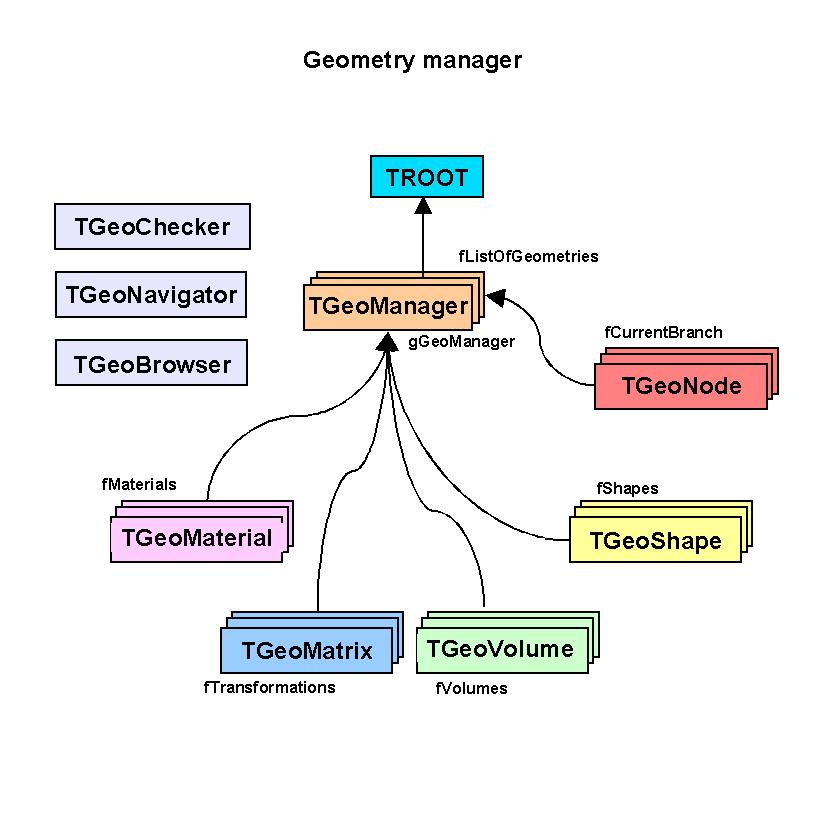
\includegraphics[width= 0.40\textwidth]{belleII_det/images/TGeoManager}
    \caption{TGeoManager Class Diagram}
\end{figure}

\paragraph{Reconstruction}
$\\$
The reconstruction process allows the particles measurement and identification. The closer the reconstructed quantities (such as initial positions and four-momenta) are to the generated-level information, the better the reconstruction performance in simulated MC and real data. Since several products of $e^+ e^-$ are short living particles, it is necessary to reconstruct them indirectly via their daughter particles. Furthermore, intrinsic noise must be taken into account, as it may generate spurious random signals unrelated to actual particles. Interactions between beam electrons or positrons, either with each other or with other accelerator components -known as beam background- must be considered.
$\\$
The same reconstruction algorithms are employed in data and MC, in order to obtain the same reconstruction: in order to test the correct response of the reconstruction, the so called \textbf{MCTruth} are use used, which basically is the generator-level Monte Carlo truth of the simulated data pool. The Monte Carlo matching (MC-matching) procedure identifies the generator-level particle responsible for a reconstructed candidate, crucial for understanding reconstruction effects and backgrounds. This corresponds to the association of reconstructed particles with MC particles in Belle II nomenclature.

\subsubsection{basf2 modules and path}
A \textbf{basf2 module} is the smallest building block of the framework and it is a script, usually written in C++, designed to process a specific unit of data. A typical data chain consists of a linear arrangement of modules. All the work is done in modules, including reading and writing data to and from disk or more complex operations such as full detector simulation.
$\\$
Modules are linearly arranged in a \textbf{path}, which is a container for them. The linear order depends on the specific task defined by the user. Therefore, the modules are executed one at a time, in the same order they were added into the path, from the first to the last. A schematic view of processing flow is shown below:

\begin{figure}[H]
    \centering
    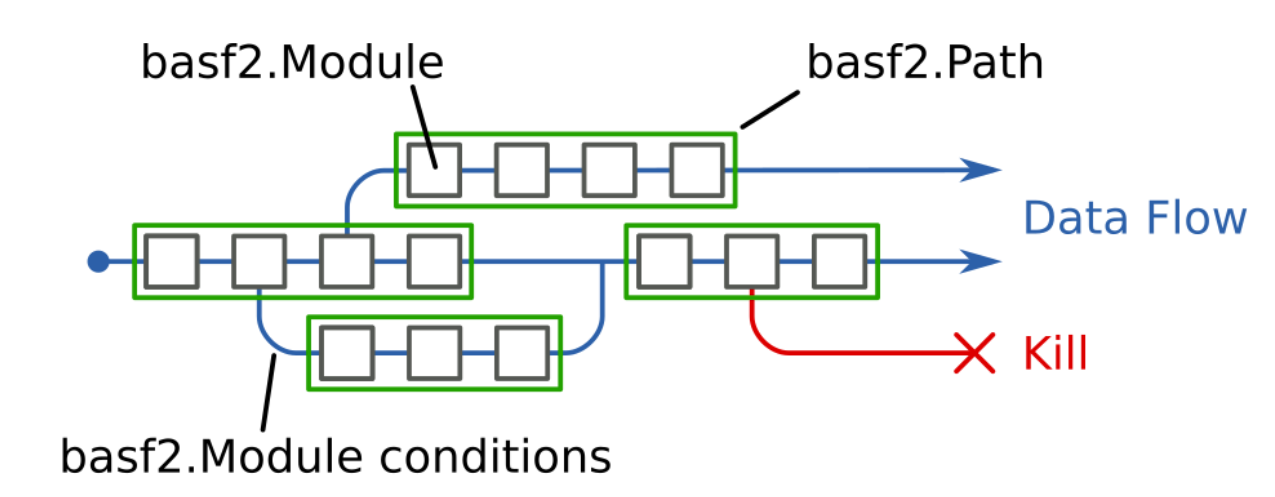
\includegraphics[width= 0.70\textwidth]{belleII_det/images/basf2_1}
    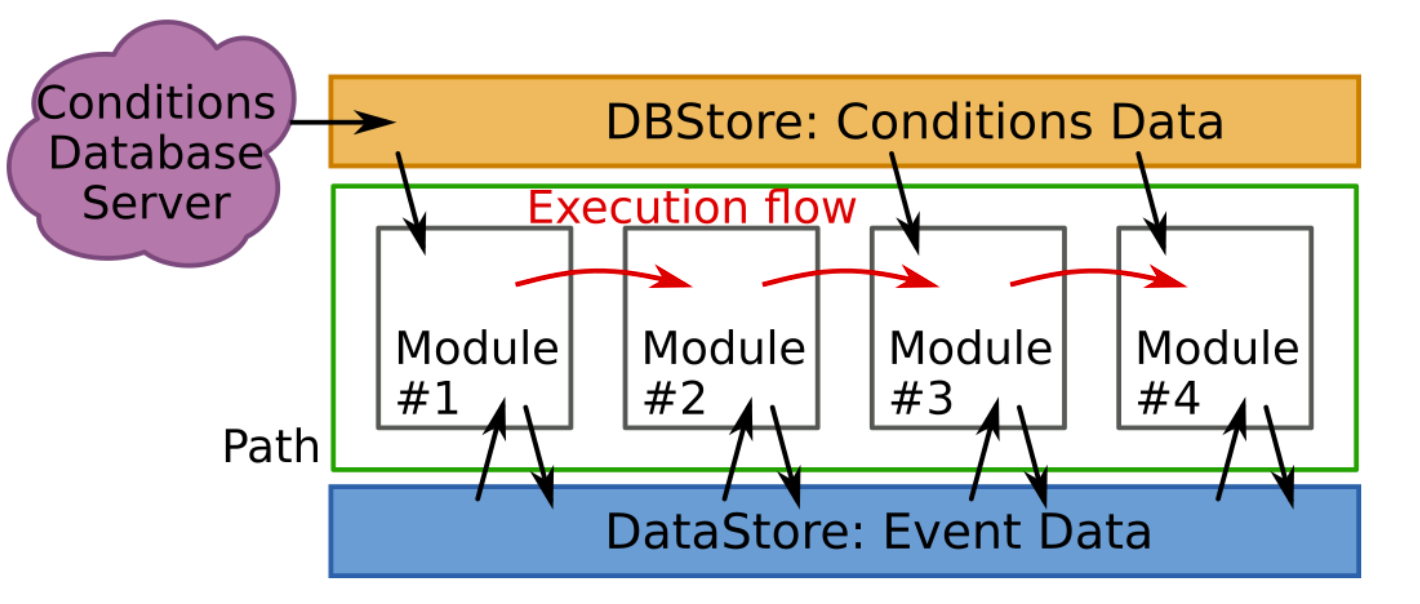
\includegraphics[width= 0.70\textwidth]{belleII_det/images/basf2_2}    
    \caption{Scheme of the processing chain in basf2}
\end{figure}

The modules process data stored in the DataStore, with each module having access to read from and write to it. There is also a non-event data, the so called conditions, which is loaded from a central conditions database and is available in the DBStore. These databases stores the information about the specific detector condition at each run of the experiment. 

A \textbf{package} is a logical collection of code in basf2, consisting of several modules and some python scripts that configure paths to do common things. The packages have meaningful name related to their specific operation (tracking, reconstruction, ecl, klm, etc...). All the packages are stored in the Belle II GitLab directory. The most used package in this thesis is the \textbf{analysis package}, which contains python functions and C++ basf2 modules, such as modularAnalysis.
$\\$
The \textbf{steering file} is the core script in which analysis and data-processing tasks are performed, with a path being declared and modules added to it. Some highlights of the steering files used are provided in the appendix.

\subsubsection{TopoAna: Topology Analysis}
In high-energy physics data analysis, a comprehensive understanding of inclusive MC samples could be crucial to select signals with higher efficiency while suppressing backgrounds. This is exactly the case of the present elaborate. 
$\\$
Knowledge of the physics processes enables identification of the main backgrounds. Selection criteria can then be further optimized by analyzing differences between these backgrounds and the signal. 

\begin{figure}[H]
    \centering
    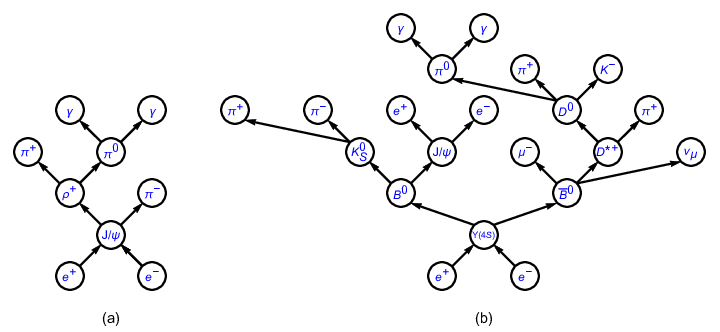
\includegraphics[width= 0.95\textwidth]{belleII_det/images/topology_diagrams}
    \caption{Topology diagrams of (a) $e^+e^-\rightarrow J/\psi$ and (b) $ e^+e^-\rightarrow \Upsilon(4S)\to B^0 \bar{B}^0$, two typical processes at $e^+ e^-$ colliders, such as Belle II and BESIII}
    \label{fig:topoproc}
\end{figure}

In order to have a very quick way to verify the Monte Carlo quickly and easily, a topology analysis program called \textbf{TopoAna} is developed with C++, ROOT, and LaTeX.
$\\$
The program input consists of one or more ROOT files containing a \textbf{TTree} object with raw topology truth information from the inclusive MC samples under study. Specifically, each \textbf{TTree} entry includes three key ingredients for particles produced in an event: the particle multiplicity, their PDG codes, and their mother indices.
$\\$
TopoAna is an offline tool independent of basf2. It independently extracts human-readable topology information from raw MC truth data via the MCGenTopo interface. Referring to figure ~\ref{fig:topoproc} (b):
\begin{figure}[H]
    \centering
    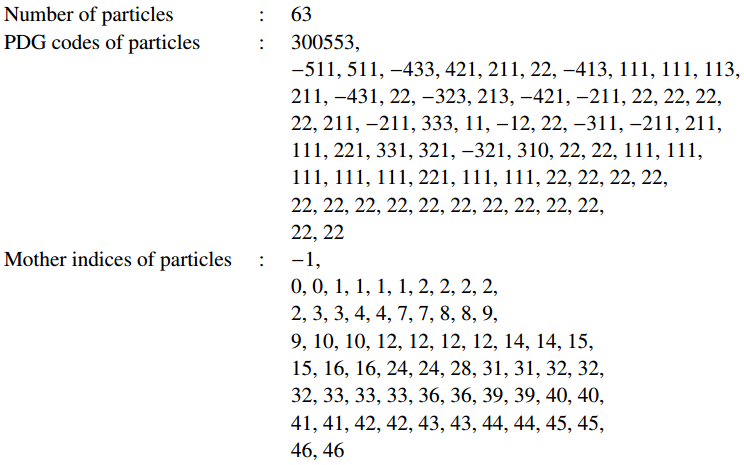
\includegraphics[width= 0.49\textwidth]{belleII_det/images/topology_diagrams_2}
     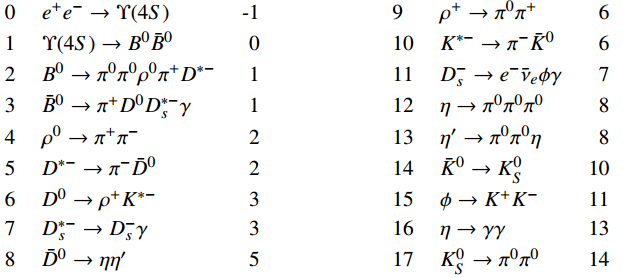
\includegraphics[width= 0.49\textwidth]{belleII_det/images/topology_diagrams_3}
    \caption{(a) Raw and (b) highly readable symbolic expressions of physics processes ~\ref{fig:topoproc} (b):}
\end{figure}


\clearpage
\setcounter{subsection}{0} 
\part{Study of the Monte Carlo signal channel}
 
The first part of the present work aims to characterize the kinematics of the $\bar{n}$, using a Monte Carlo signal sample generated specifically for the selected reference channel:  

\begin{center}
$e^+ \ + \  e^- \rightarrow p \ + \ \pi^- \ + \ \bar{n} \  (+ \ \gamma_{\rm ISR})$
\end{center}

This is selected because it features simple kinematics, with the $\bar{n}$ as the only missing particle, enabling a semi-exclusive analysis. 
$\\$
The Feynman diagram for this process, without and with ISR emission, is shown in Fig.~\ref{fig:diag_F}.


\begin{figure}[H]
    \centering
    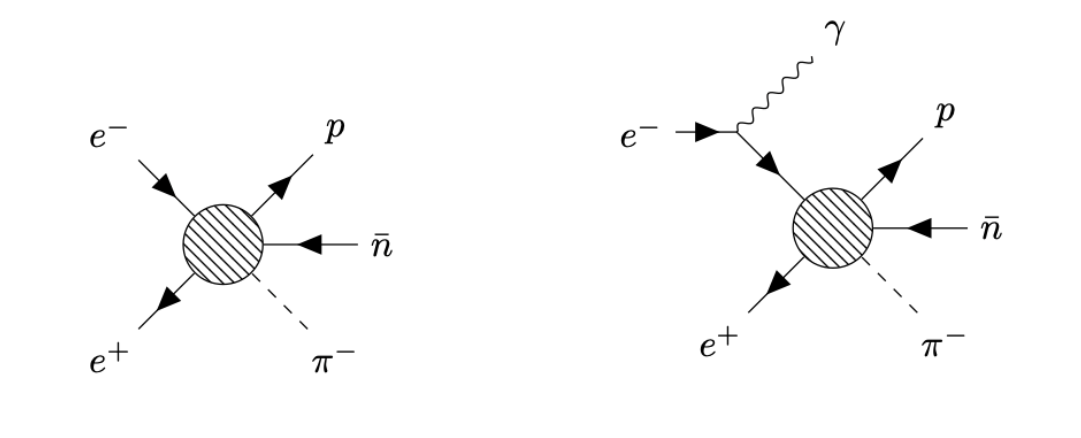
\includegraphics[width=1\textwidth]{nbar_MC/images/channel_art}
    \caption{Feynman Diagram of the channel of interest. The ISR gamma is a pre-interaction radiation emitted by the $e^+$ and/or $e^-$. The recoil system is made of $p \pi^- (\gamma_{ISR})$.}
    \label{fig:diag_F}
\end{figure}

In particular, the kinematic relation between the $\bar{n}$ and the recoil system $p \pi^- (\gamma_{ISR})$ will be exploited, considering both configurations: in the presence of Initial State Radiation (ISR) photon emission and in its absence. ISR corresponds to the emission of photons from incoming particles before they collide in high-energy physics experiments. This reduces the effective center-of-mass energy available, which will no longer be $\sim 10.58$ GeV, in the Belle II case. The ISR energy and angle distributions will be discussed in detail, providing a comparison with a simple phase space model emission.
$\\$
Then, the effect of a one constraint (1C) kinematic fit over the recoil mass will be discussed, in order to obtain a higher recoil momentum resolution.
$\\$
In total, 100000 events are generated and to perform the event generation and the analysis,  \textbf{basf2} is employed. Script code highlights for this section are shown in Appendix~\hyperref[app:A]{\ref*{app:A}}, where the decay file, MC generation file, and steering file are explained in detail.
$\\$
The basf2 \textbf{Phokhara\_evtgen\_combination} generator has been adopted. It is made of two generators: \textbf{Phokhara} and \textbf{EvtGen}.
$\\$
Phokhara is a Monte Carlo event generator that simulates $e^+e^-$ annihilation into hadrons at next-to-leading order (NLO) accuracy. This includes virtual and soft photon corrections to single-photon events, plus double hard photon emission. 
$\\$
EvtGen is a Monte Carlo event generator that simulates decays of heavy-flavor particles, primarily B and D mesons. It includes decay models for intermediate and final states with scalar, vector, and tensor mesons/resonances, as well as leptons, photons, and baryons. Decay amplitudes generate each branch of the full decay tree, accounting for angular and time-dependent correlations to simulate CP-violating processes.
$\\$
Therefore, these two generators have been adopted as depicted in Fig.~\ref{fig:diag_F_colors}.

\begin{figure}[H]
    \centering
    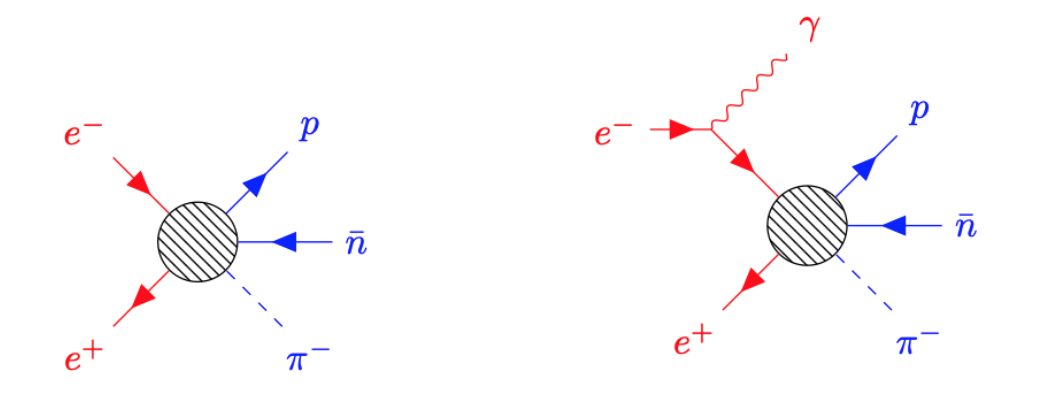
\includegraphics[width=1\textwidth]{nbar_MC/images/channel_art_colors}
    \caption{Feynman diagram of the channel of interest. \textit{Phokhara} handles the initial hard photon emission (red), while \textit{EvtGen} simulates the decay to final-state particles (blue).}
    \label{fig:diag_F_colors}
\end{figure}
Importantly, the Phokhara\_evtgen\_combination generator produces both events with and without ISR emission, as explicitly illustrated by the TopoAna overview of generated events in Fig.~\ref{fig:topo_signal0}.
$\\$
A $vpho$ (virtual photon) is now introduced as a fictitious particle used by the generator Phokhara to produce ISR photons before the $e^+ e^-$ collisions and then enforce (evt\_gen) the selected decay channel, approaching the following scheme:

\begin{center}
$e^+ \ + \  e^- \rightarrow vpho +  \ \gamma_{ISR} $ (Phokhara generator)

\vspace{0.3cm}

$vpho \rightarrow p \ + \ \pi^- \ + \ \bar{n} $ (EvtGen generator)
\end{center}
Figuratively, it can be represented as the blob shown in the Feynman diagram.

\subsection{Kinematic variables comparison}
Two scenarios can be studied. If the reconstructed final state particles are a proton ($p$), a negative pion ($\pi^-$) and an anti-neutron ($\bar{n}$), it is referred to as the \textbf{NO ISR case}. If the ISR photon ($\gamma_\text{ISR}$) is also reconstructed, it is referred to as the \textbf{ISR case}. Therefore, in the NO ISR case, the recoil system is defined as the $p\pi^-$ system, while in the ISR case it is defined as the $p\pi^-\gamma_\text{ISR}$ system. 

\begin{figure}[H]
    \centering
    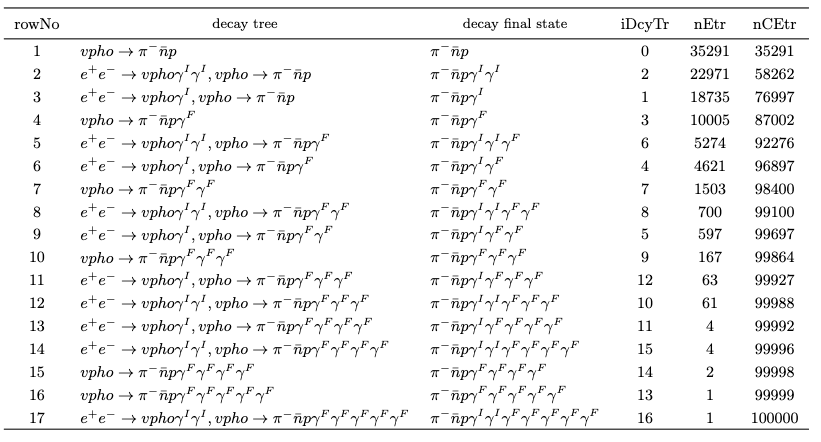
\includegraphics[width=1\textwidth]{nbar_MC/images/topoana_100k}
    \caption{Topology Analysis (TopoAna) output of the generated 100k events. The fourth column is the unambiguous decay tree index associated to the correspondent channel, the fifth the number of entries per channel, and the last the cumulative number of entries.}
    \label{fig:topo_signal0}
\end{figure}

As a first step, the kinematic variables are discussed through the recoil system consisting of $p \pi^- (\gamma_{ISR})$, where these particles are reconstructed. In parallel, the neutral $\bar{n}$ cluster candidate is reconstructed and its properties are compared to those from the recoil, comparing different kinematic variables. Through the recoil analysis, the antineutron can be identified as the missing particle in the final state.
$\\$
The first three contributes in Fig.~\ref{fig:topo_signal0} shows that events without ISR emission are the most frequently generated ($\sim 35\%$), followed by those with two ($\gamma^I\gamma^I$) ($\sim 23\%$) and one ($\gamma^I$) ISR photon ($\sim 19\%$). 
$\\$
Additionally, numerous Final State Radiation (FSR) photons are emitted by the charged final state particles due to next order perturbative QED processes.

\subsubsection{ISR distributions}
The ISR energy and angular distributions are discussed below. The primary effect of ISR emission is the reduction of the center-of-mass energy $\sqrt{s}$ below the $\Upsilon(4S)$ resonance.
$\\$
Therefore, the energy E and $\theta$ distributions of ISR radiation are shown if Fig.~\ref{fig:isr_distro}.
\begin{figure}[H]
    \centering
    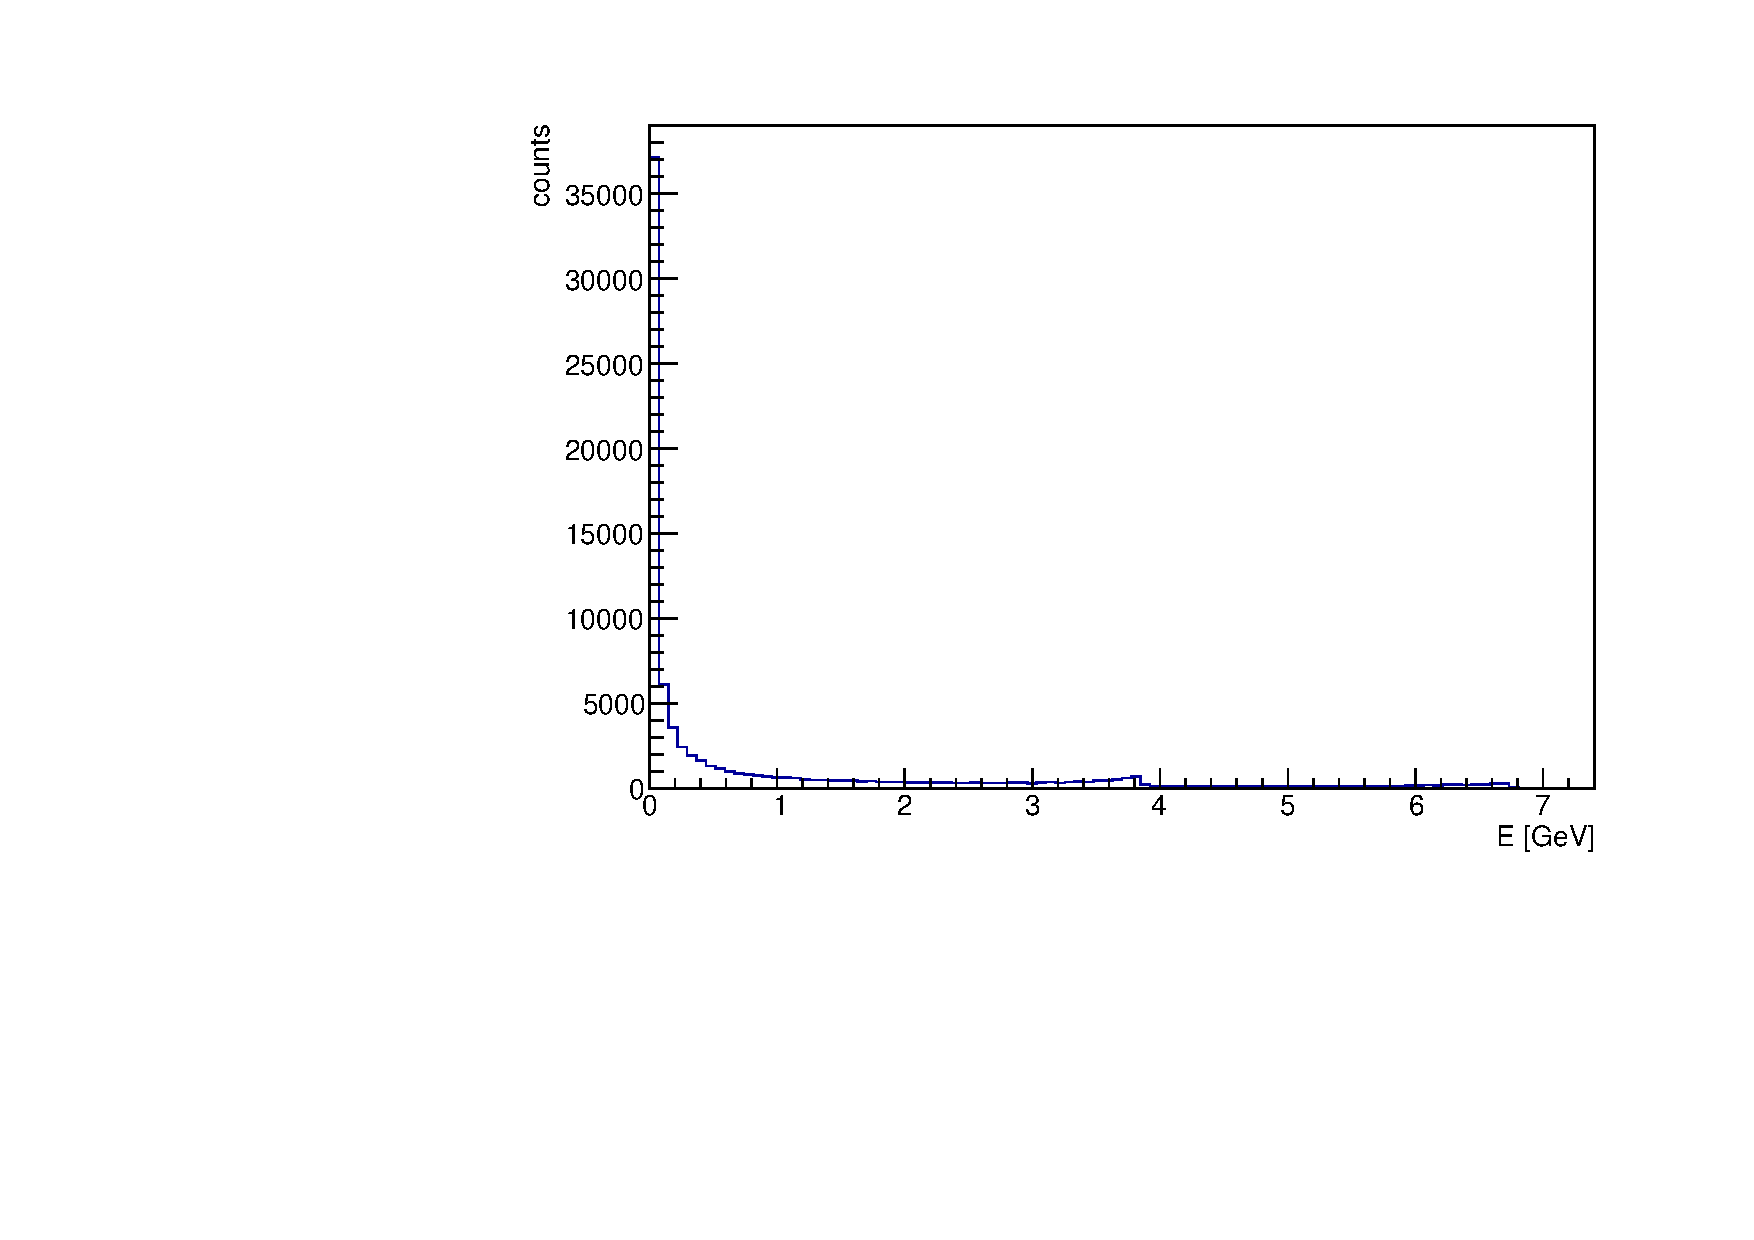
\includegraphics[width=0.49\textwidth]{nbar_MC/images/ISR_energy.pdf}
    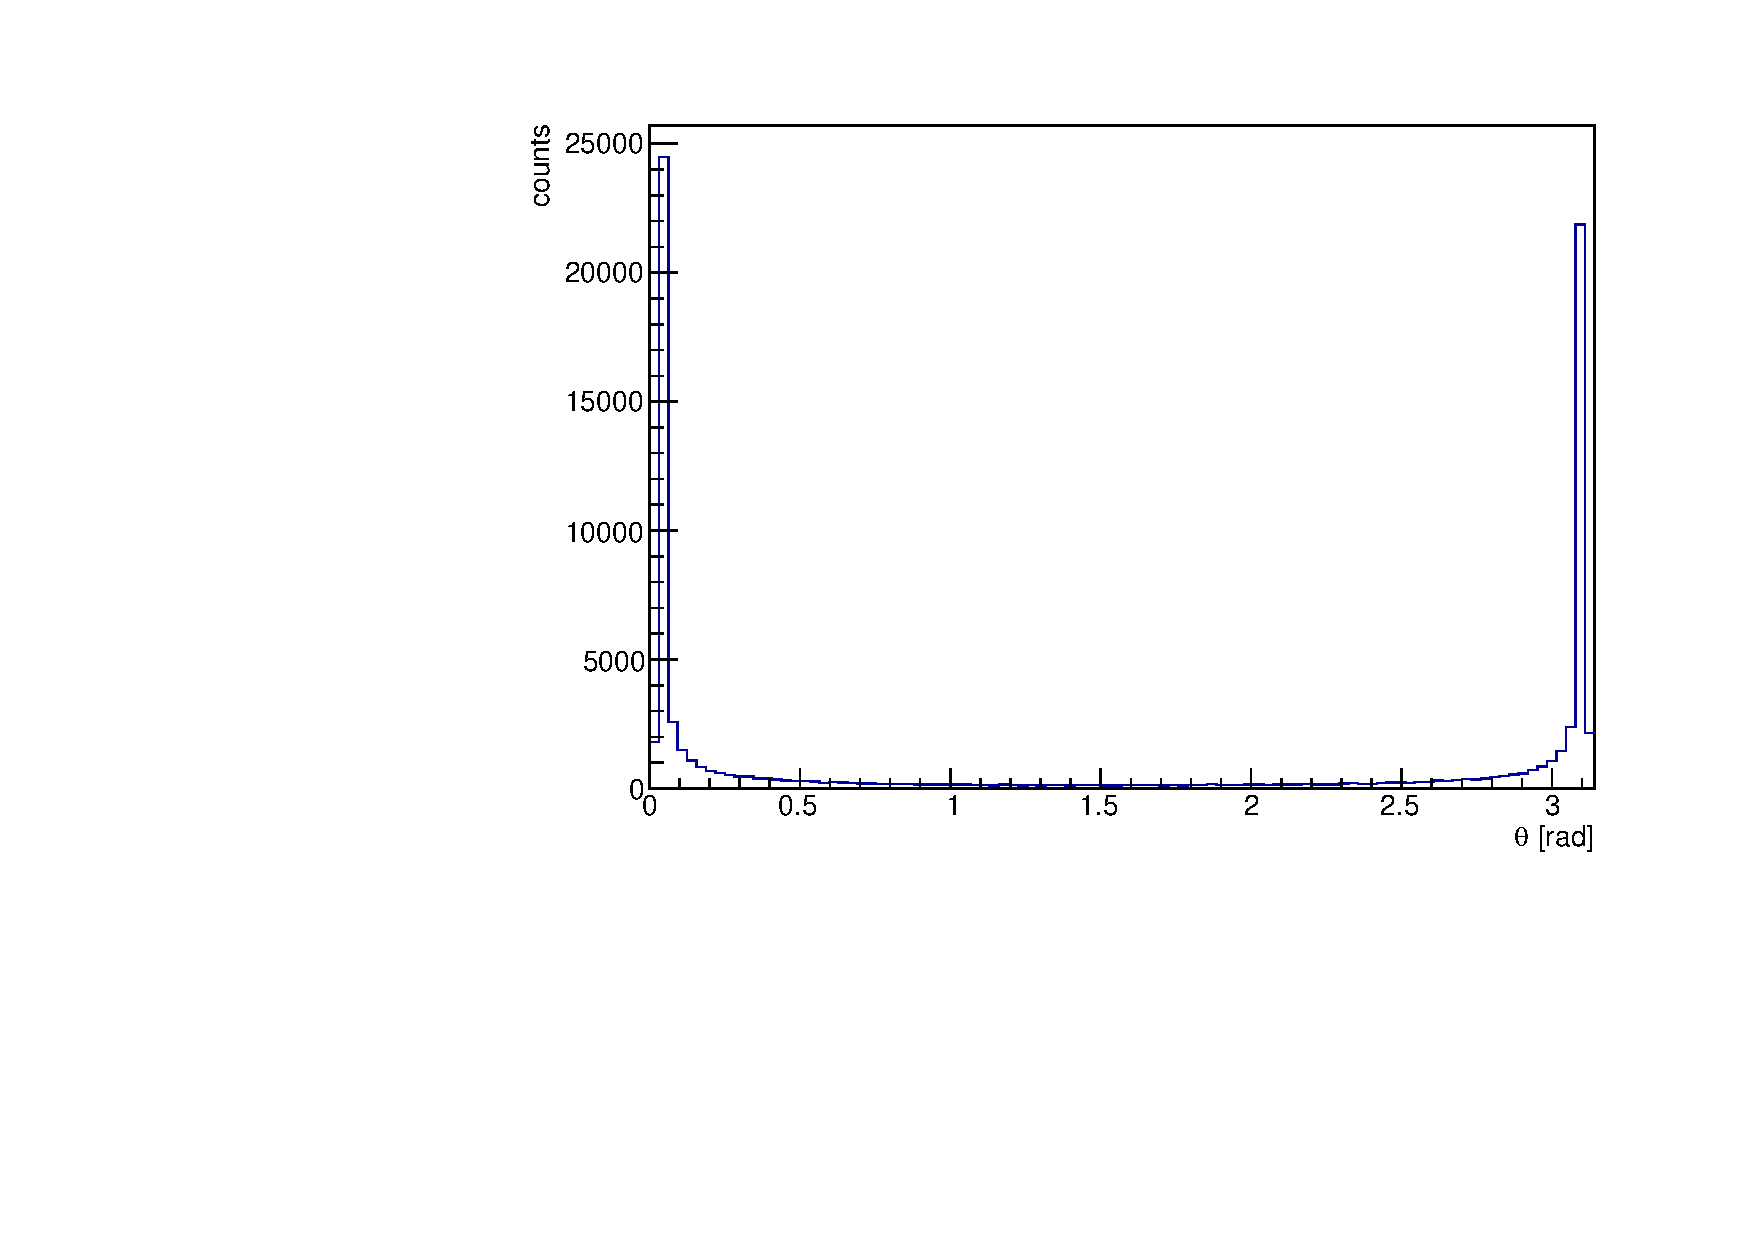
\includegraphics[width=0.49\textwidth]{nbar_MC/images/ISR_theta.pdf}
    \caption{(a) ISR energy distribution. (b) ISR $\theta$ distribution. Both distributions are shown on a logarithmic $y$-axis scale.}
    \label{fig:isr_distro}
\end{figure}

The conjugate energy E and $\theta$ distribution of ISR radiation are shown if Fig.~\ref{fig:isr_distro_conj}.
\begin{figure}[H]
    \centering
    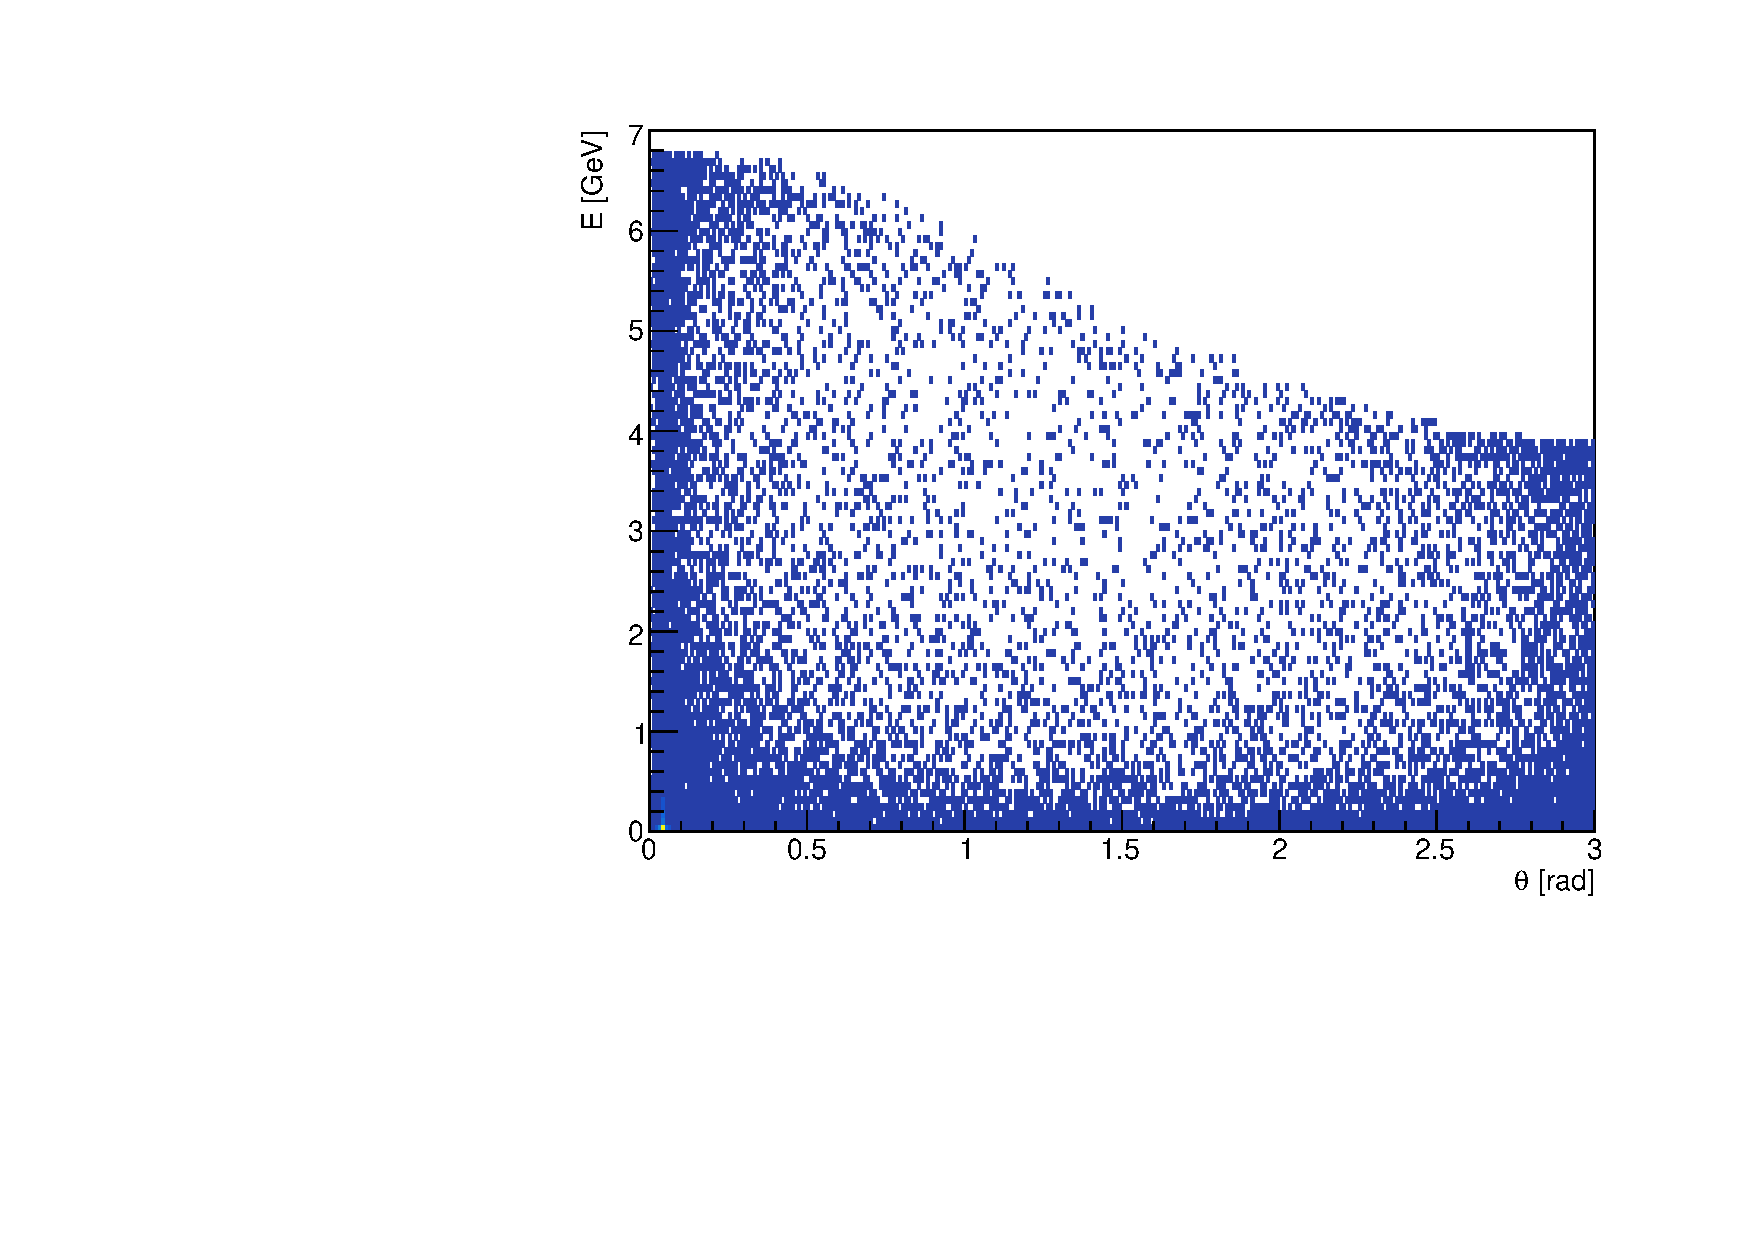
\includegraphics[width=0.70\textwidth]{nbar_MC/images/ISR_energy_vs_theta.pdf}
    \caption{Conjugate energy E and $\theta$ distribution of ISR radiation.}
    \label{fig:isr_distro_conj}
\end{figure}

The ISR energy distribution mainly consists of photons in the $[0,1]$ GeV energy. Two peaks are observed slightly below 4 GeV and 7 GeV, corresponding to the energies of the $e^+$ and $e^-$ beams, respectively. The angular distribution present a U-shape, indicating that forward and backward directions are the most probable. 
$\\$
Furthermore, as can be observed in Fig.~\ref{fig:isr_distro_conj}, the higher the energy of the ISR radiation, the closer $|cos(\theta)|$ is to 1, indicating that high-energy $\gamma_{ISR}$ photons are emitted preferentially in the forward and backward directions. The peak at low $\theta$ values (forward direction) is higher than the backward peak, consistent with the detector asymmetry with respect to the interaction point.

\subsubsection{Event selections}
In the ISR case, the final state $p\pi^-\bar{n}\gamma_\text{ISR}$ is reconstructed; the recoil of $p\pi^-\gamma_{ISR}$ is then built. In the NO ISR case, the final state $p\pi^-\bar{n}$ is reconstructed; the recoil of $p\pi^-$ is then built. Therefore, the $\bar{n}$ can be identified through the recoil mass peak at the anti-neutron mass. 
$\\$
To properly select the signal in the recoil mass distribution, several cuts are applied in the steering file as follows:

\begin{enumerate}
\item Recoil system: $0 \ GeV/c^2 <recoil \ mass < 2 \ GeV/c^2$
\item $\bar{n}$: neutral clusters from ECL
\item $p$: $protonID > 0.9$ and $dr<1$ cm and $|dz|<3$ cm 
\item $\pi^-$: $pionID > 0.1$ and $dr<1$ cm and $|dz|<3$ cm 
\end{enumerate}

The first one is a cut that selects the region of interest in the recoil mass distribution, corresponding to the interval [0,2] $GeV/c^2$ around the antineutron mass ($\sim 939,56$ $MeV/c^2$). 
$\\$
To analyze only $\bar{n}$ signals from the calorimeter, the second selection requires that the neutral $\bar{n}$ cluster candidates are reconstructed within the electromagnetic calorimeter (ECL), avoiding the $\bar{n}$ candidates from other detectors (mainly from KLM).
$\\$
The third and fourth criteria are standard selections recommended by the basf2 framework. The ID requirement imposes a constraint on the protonID or pionID based on a maximum likelihood criterion as follows:
\begin{center}
$protonID = \frac{L_p}{L_e + L{\mu} + L{\pi} +L_K + L_d }$
\hspace{0.3cm}
$pionID = \frac{L_\pi}{L_e + L{\mu} + L{p} +L_K + L_d }$,
\end{center}
where $L_p$ is the likelihood for the proton hypothesis, $L_{\pi}$ is the likelihood for the pion hypothesis, and so on.
$\\$
The cuts on $dr$ and $|dz|$ select only tracks originating from the interaction point (IP) area, where $dr$ is defined as the transverse distance with respect to IP and $dz$ is defined as the axial distance, along the z-axis, with respect to IP.
$\\$
Since multiple $\bar{n}$ neutral cluster candidates may exist per event, only the candidate with the smallest angle -defined as $\alpha$- relative to the recoil system is selected. Therefore, a selection is imposed using the basf2 \textbf{rankByLowest} method. It allows to select only the highest rank candidates, based on a specific variable; in this case, the angle between the neutral cluster and the recoil vector.
$\\$
Using spherical coordinate system, after some algebraic steps, the 3D angle $\alpha$ between the two vectors can be obtained:

\begin{center}
$\alpha = arcos[sin(\theta_1)sin(\theta_2)cos(\phi_1 - \phi_2) + cos(\theta_1)cos(\theta_2) ]$
\end{center}

Here vector \textbf{1} denotes the recoil vector and the vector \textbf{2} denotes the $\bar{n}$ direction vector. The respective $\alpha$ distributions, before and after the aforementioned selection, are shown in Fig.~\ref{fig:alpha_pre_post}, in both ISR and NO ISR cases:

\begin{figure}[H]
    \centering
    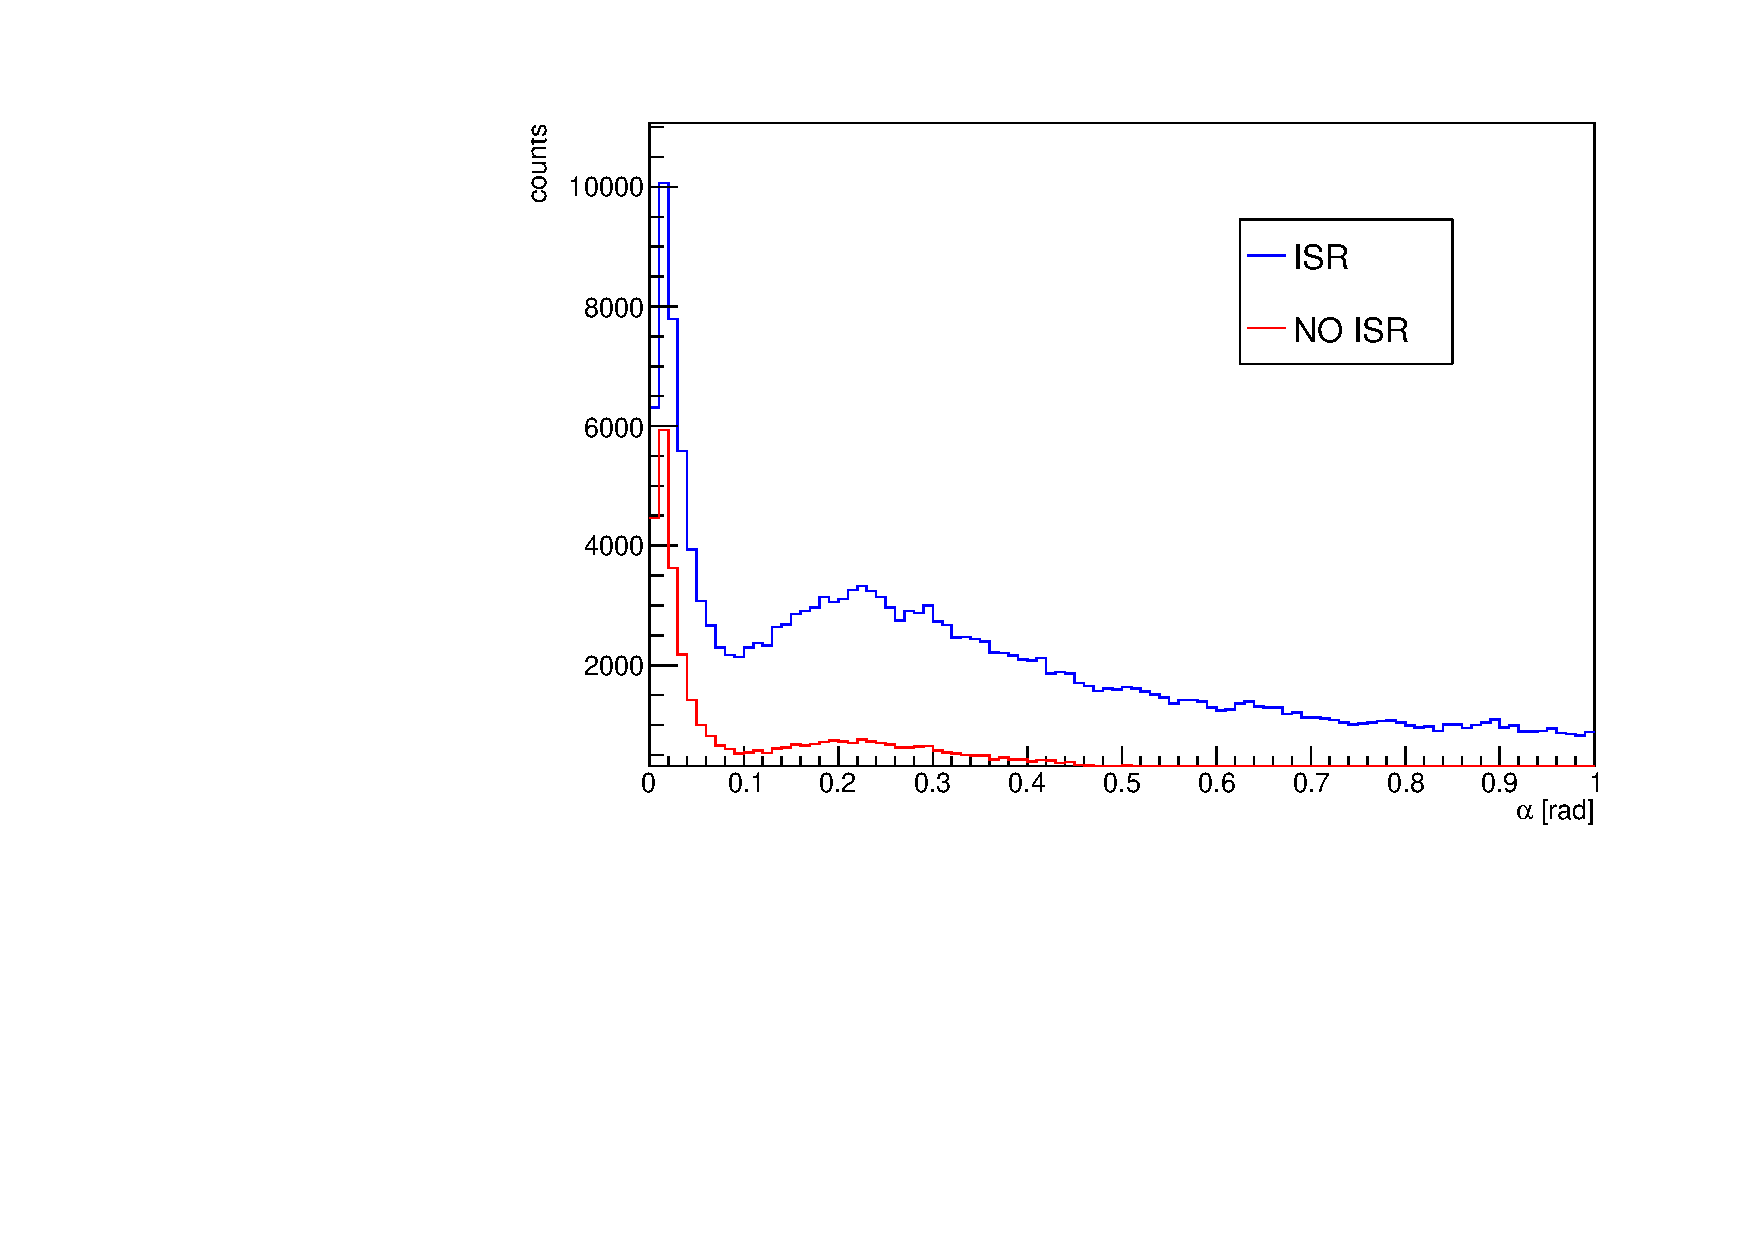
\includegraphics[width=0.49\textwidth]{nbar_MC/images/alpha_uncorr.pdf}
    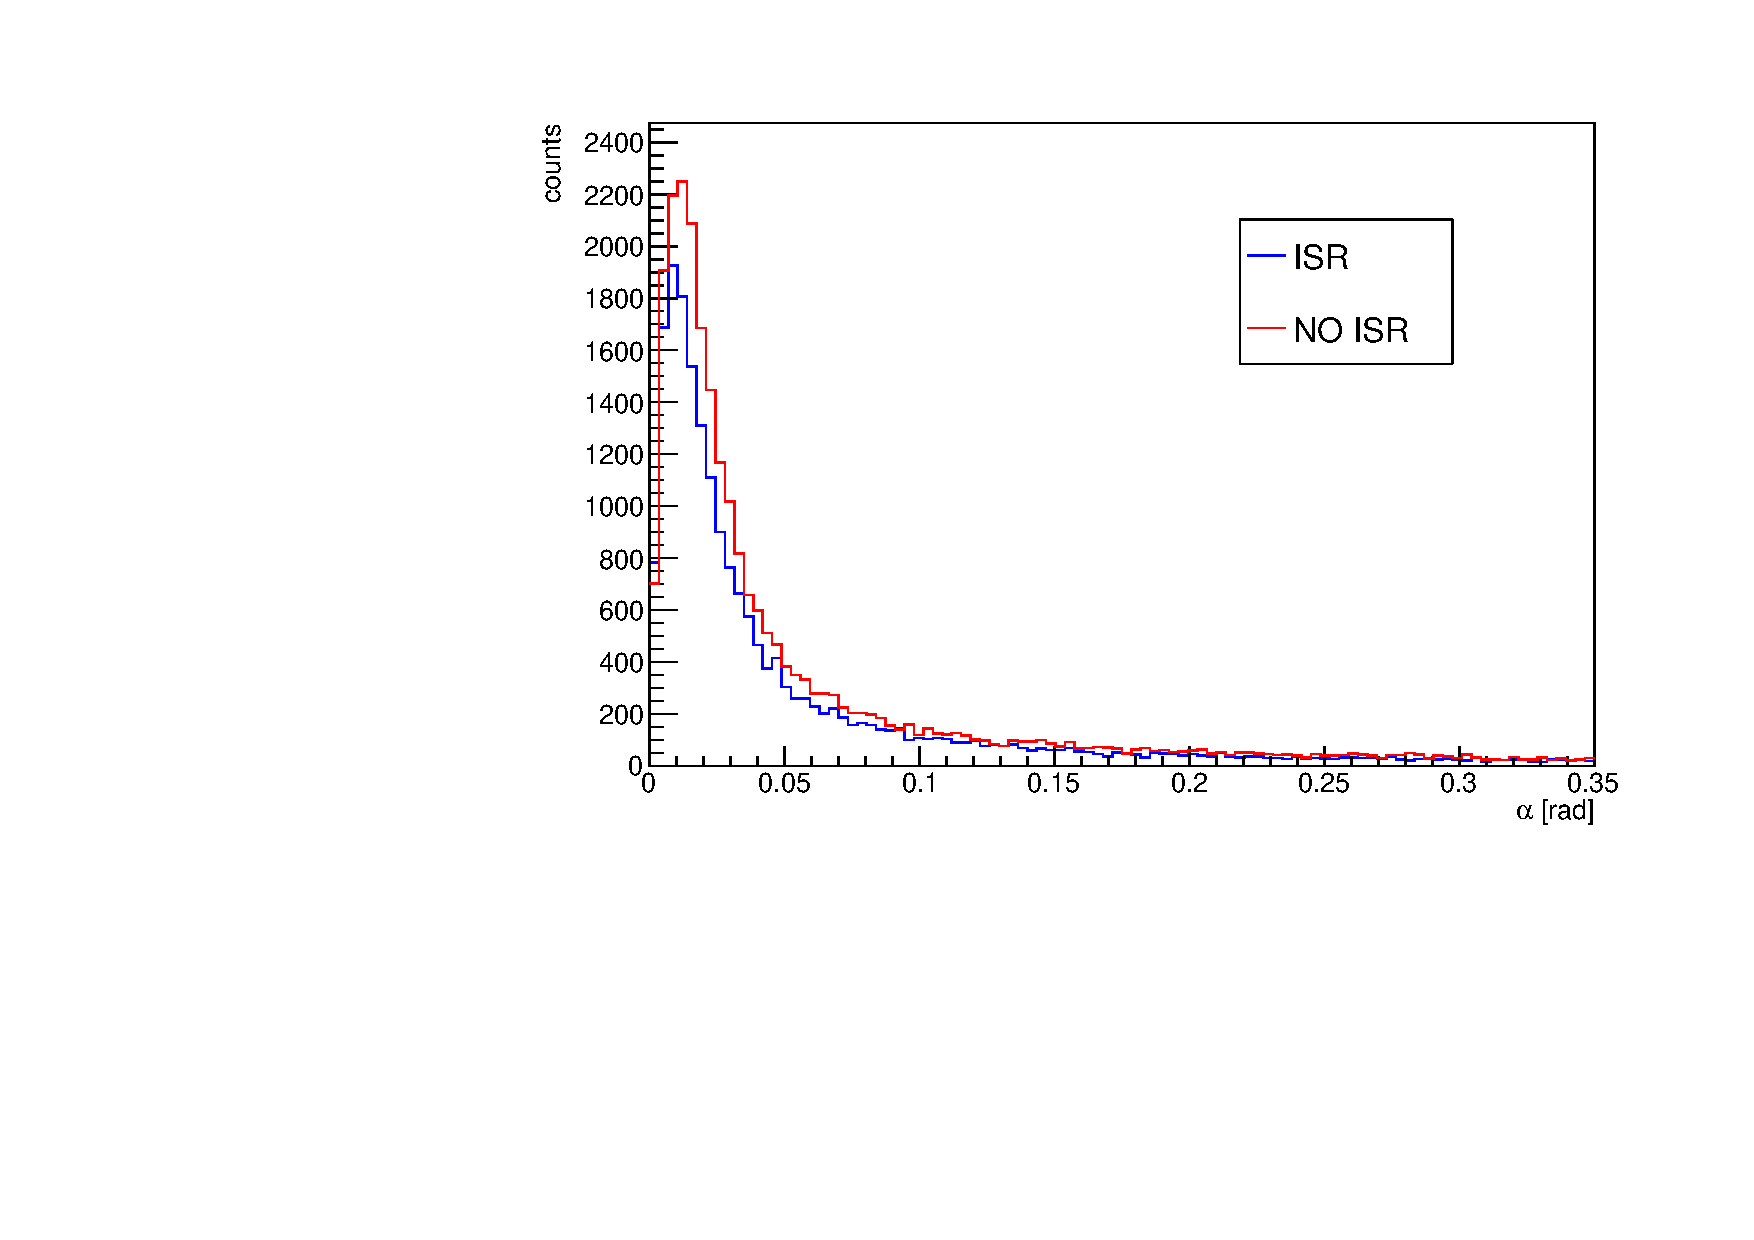
\includegraphics[width=0.49\textwidth]{nbar_MC/images/alpha.pdf}
    \caption{(a) $\alpha$ distribution. (b) $\alpha$ distribution after the rank selection.}
    \label{fig:alpha_pre_post}
\end{figure}

To select the most probable $\bar{n}$ candidates, only those with $\alpha < 0.35$ ($\sim 20^\circ$) are stored.
$\\$
The efficiency $\epsilon$  is defined as follows:
\begin{center}
  $\epsilon = \frac{n^{\circ} \ of \ reconstructed \ candidates}{n^{\circ}  \ of \ generated \ events} $
\end{center}

Referring to Fig.~\ref{fig:topo_signal0}, 46969 events are generated without ISR emission ($iDcyTr \in {0,3,7,9,14,13}$) and 53031 with ISR emission ($iDcyTr \in {2,1,6,4,8,5,12,10,11,15,16}$) .
$\\$
Since 20146 candidates are reconstructed for the ISR case and 25013 for the NO ISR case, an efficiency respectively of $\sim 53\%$ and $38\%$ can be observed.
Since most of the ISR radiation is emitted in the backward ($\theta \sim 180^{\circ}$) and in the forward ($\theta \sim 0^{\circ}$) directions -where detection coverage is absent- the efficiency in the ISR case is slightly lower than in the NO ISR case.

\subsubsection{Recoil mass distribution}
To select events with anti-neutron, the recoil system $p \pi^- (\gamma_{ISR})$ is studied through the recoil mass. Specifically, the recoil mass should peak at the nominal anti-neutron mass, since no background channels are present in this sample. The only background consists of secondary particles produced during the propagation of primary particles through the detectors. 
$\\$
The recoil mass distribution, for both ISR and NO ISR cases, is shown in Fig.~\ref{fig:recMass_distro_isr_noisr}.

\begin{figure}[H]
    \centering
    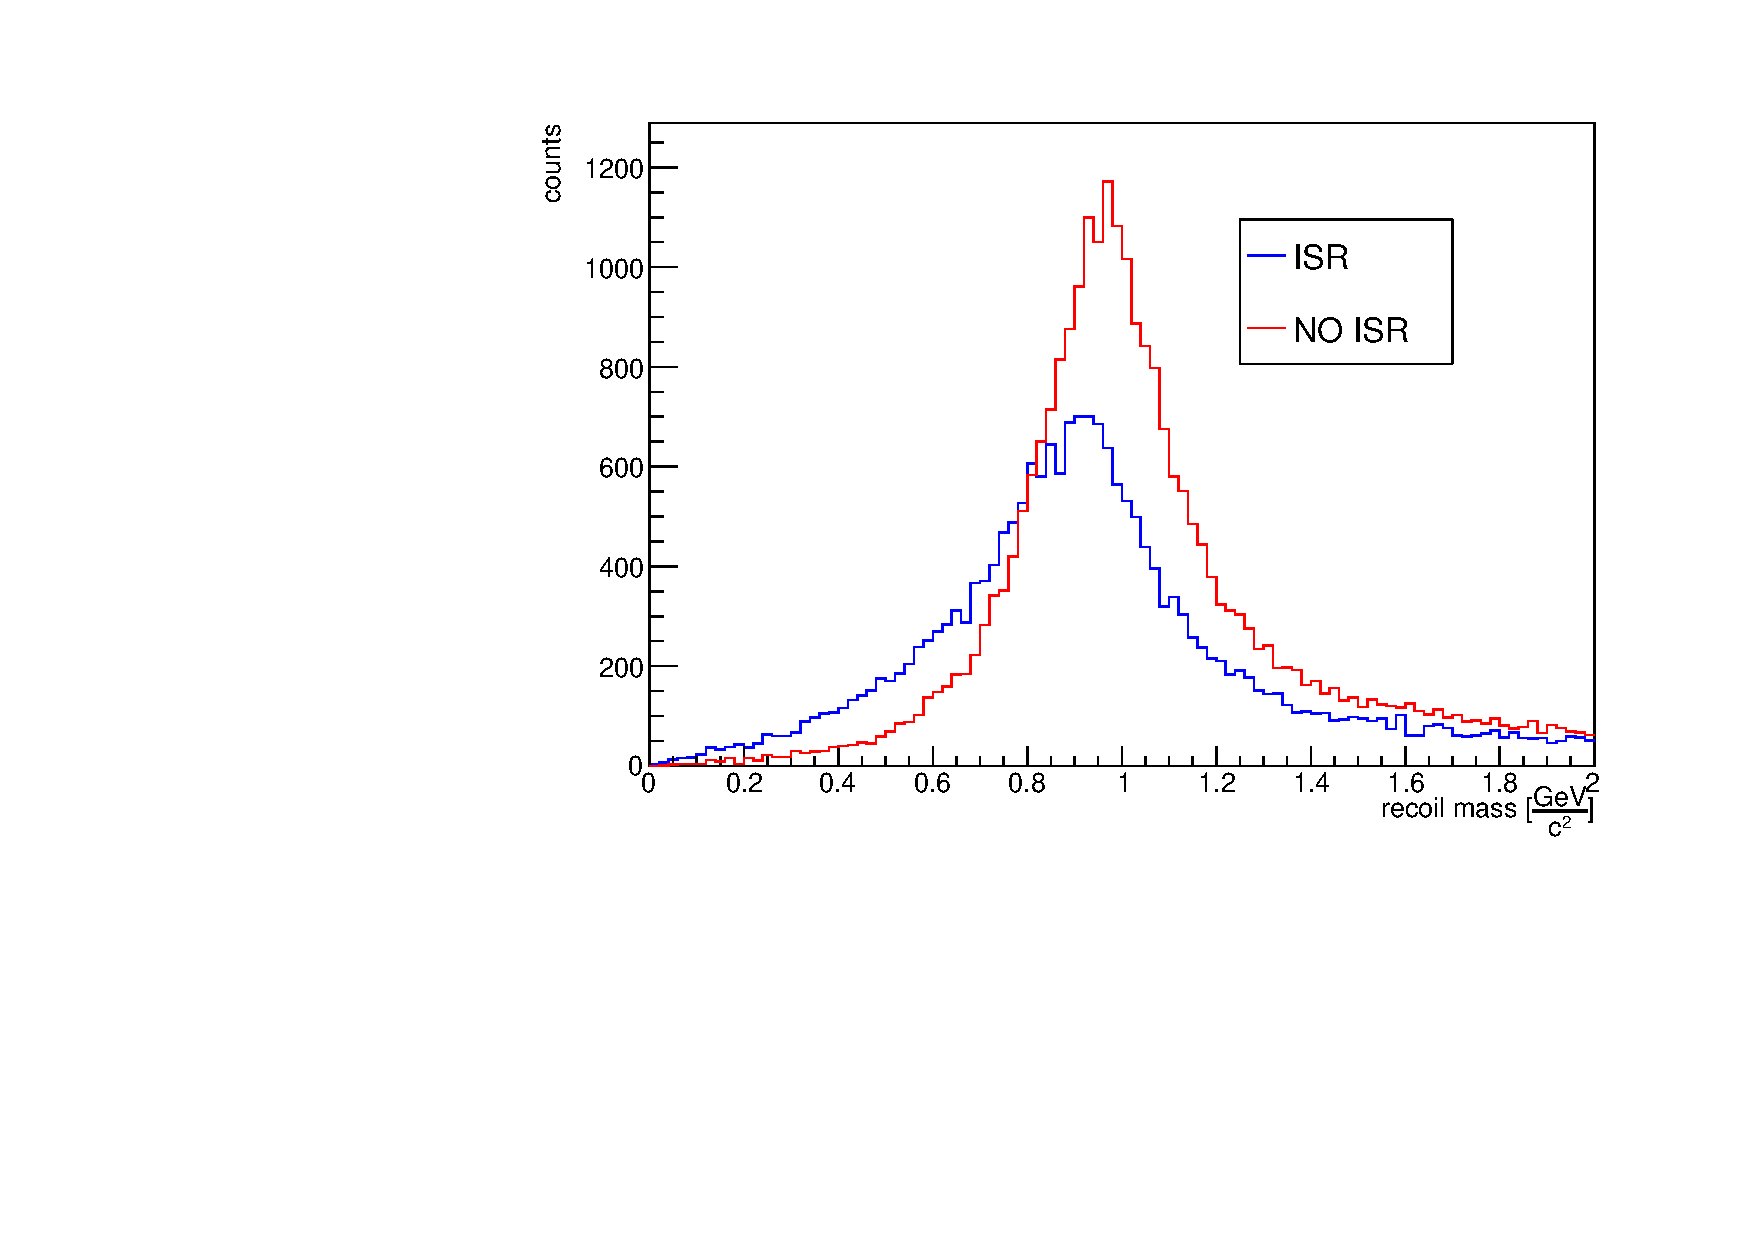
\includegraphics[width=0.7\textwidth]{nbar_MC/images/vpho_mRecoil.pdf}
    \caption{Recoil mass distribution, in both ISR and NO ISR cases.}
    \label{fig:recMass_distro_isr_noisr}
\end{figure}

The recoil mass distribution peaks on the $\bar{n}$ mass ($\sim 939.56$ MeV), indicating that the the recoil mass is well reconstructed in both ISR ($p \ \pi^-  \ \gamma_{ISR}$) and NO ISR ($p \ \pi^-$) cases. Therefore, the variables associated with the $\bar{n}$ clusters can be compared with the reconstructed recoil variables ($p, \ \theta$).
$\\$
In the event simulation the generator produces more than one $\gamma_{ISR}$ per event, reflecting into the obtained recoil mass distribution; the one obtained in ISR case shows more entries in the left tail, since only the most energetic gamma is considered in the recoil reconstruction, while the others are not considered. 
$\\$
The distribution obtained in the NO ISR case exhibits a higher peak as the recoil system reconstruction consists only of $p\pi^-$, allowing better resolution than the ISR case, since fewer tracks are considered.
$\\$
By selecting events around the peak, $\bar{n}$ candidates events can be identified. The recoil direction is expected to provide a good estimate of the $\bar{n}$ momentum.

\subsubsection{The recoil kinematic}
Before analyzing the recoil momentum distribution, the reconstructed momentum of each particle composing the recoil system is examined. For particles with MC association, the MC variables can be studied for a given list of candidates as well. 
$\\$
For example, considering the proton candidate list, both the \textbf{reconstructed} momentum of the proton list and the Monte Carlo (\textbf{generated}) momentum of the proton list -which is not affected by the reconstruction process- are available. The latter will be referred to as the "generated" momentum.
$\\$
Since a candidate list is the result of the reconstruction process, it also contains particles that have been mis-identified as the main particle (for example, $\pi^+$ mis-identified as $p$ or $\gamma$ mis-identified as $\bar{n}$).
$\\$
Therefore, the considered "generated" variables represent the Monte Carlo values for a given reconstructed particle list, which differs from the Monte Carlo values for a generator-level particle list that contains only the selected particle type.

The relative reconstructed momenta are shown in FIg.~\ref{fig:rec_p_pi_mom}.

\begin{figure}[H]
    \centering
    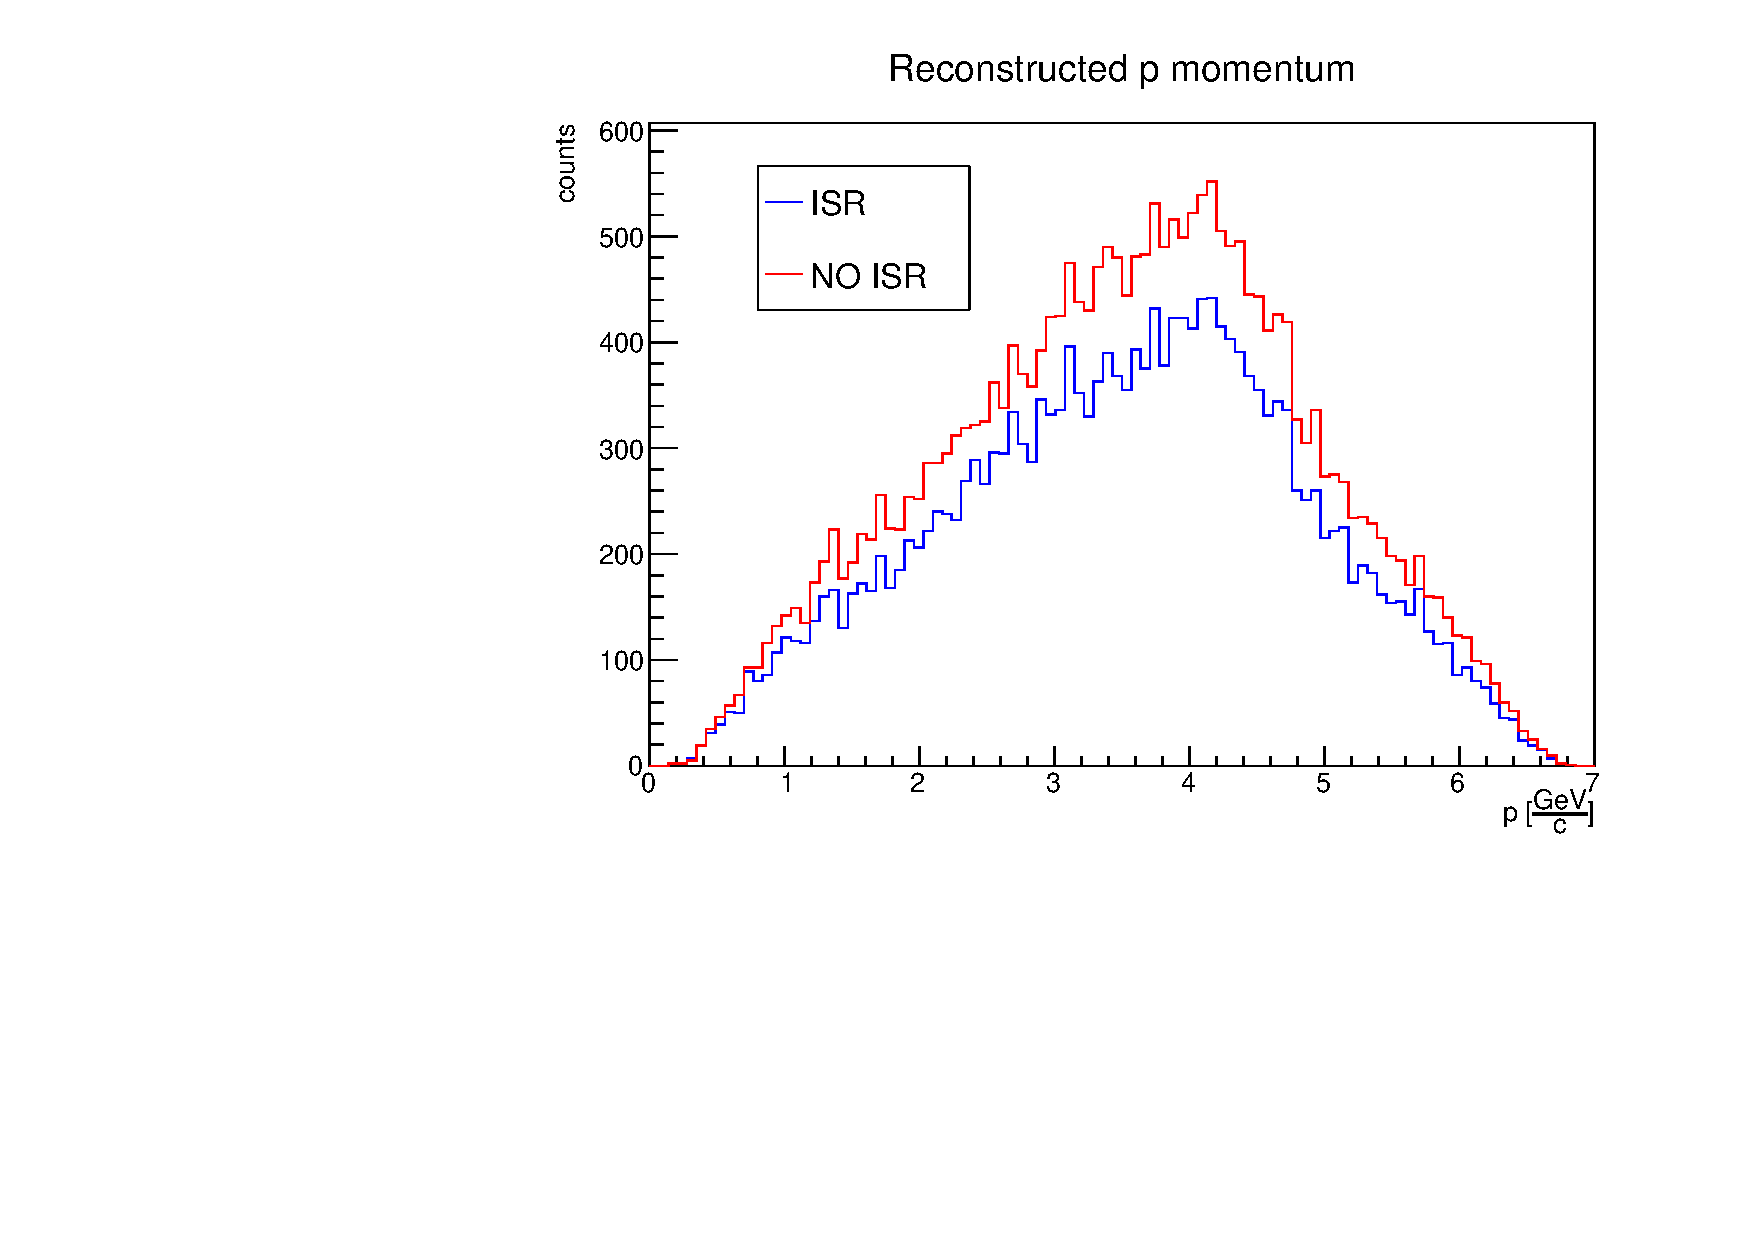
\includegraphics[width=0.49\textwidth]{nbar_MC/images/p_p.pdf}
    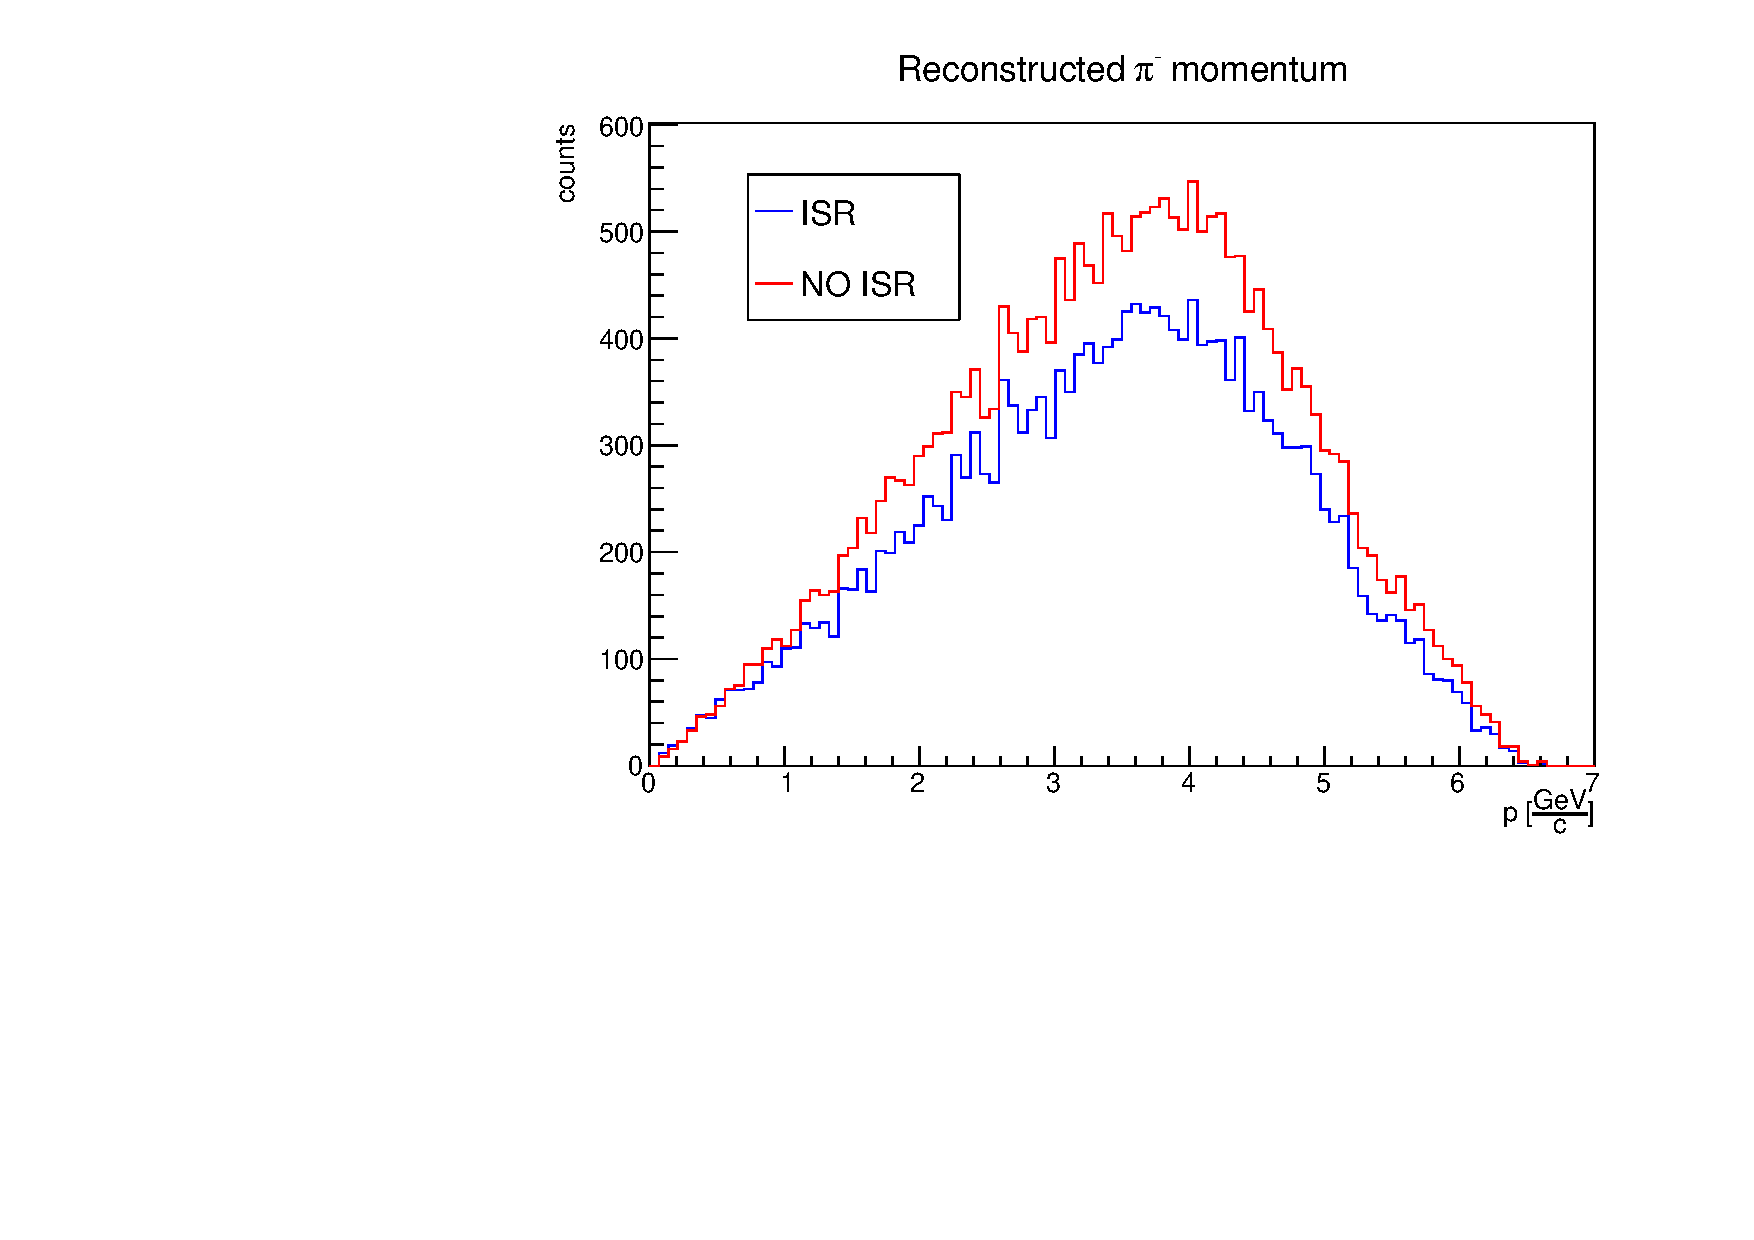
\includegraphics[width=0.49\textwidth]{nbar_MC/images/pi_p.pdf}
    \caption{Reconstructed momentum distribution of proton and pion, in both ISR and NO ISR cases}
    \label{fig:rec_p_pi_mom}
\end{figure}

The distributions clearly exhibit the typical phase-space shapes, as expected from the adopted generator model (\hyperref[app:A]{Appendix~\ref*{app:A}}). Similarly, these distributions can be obtained directly at the generator level, yielding:

\begin{figure}[H]
    \centering
    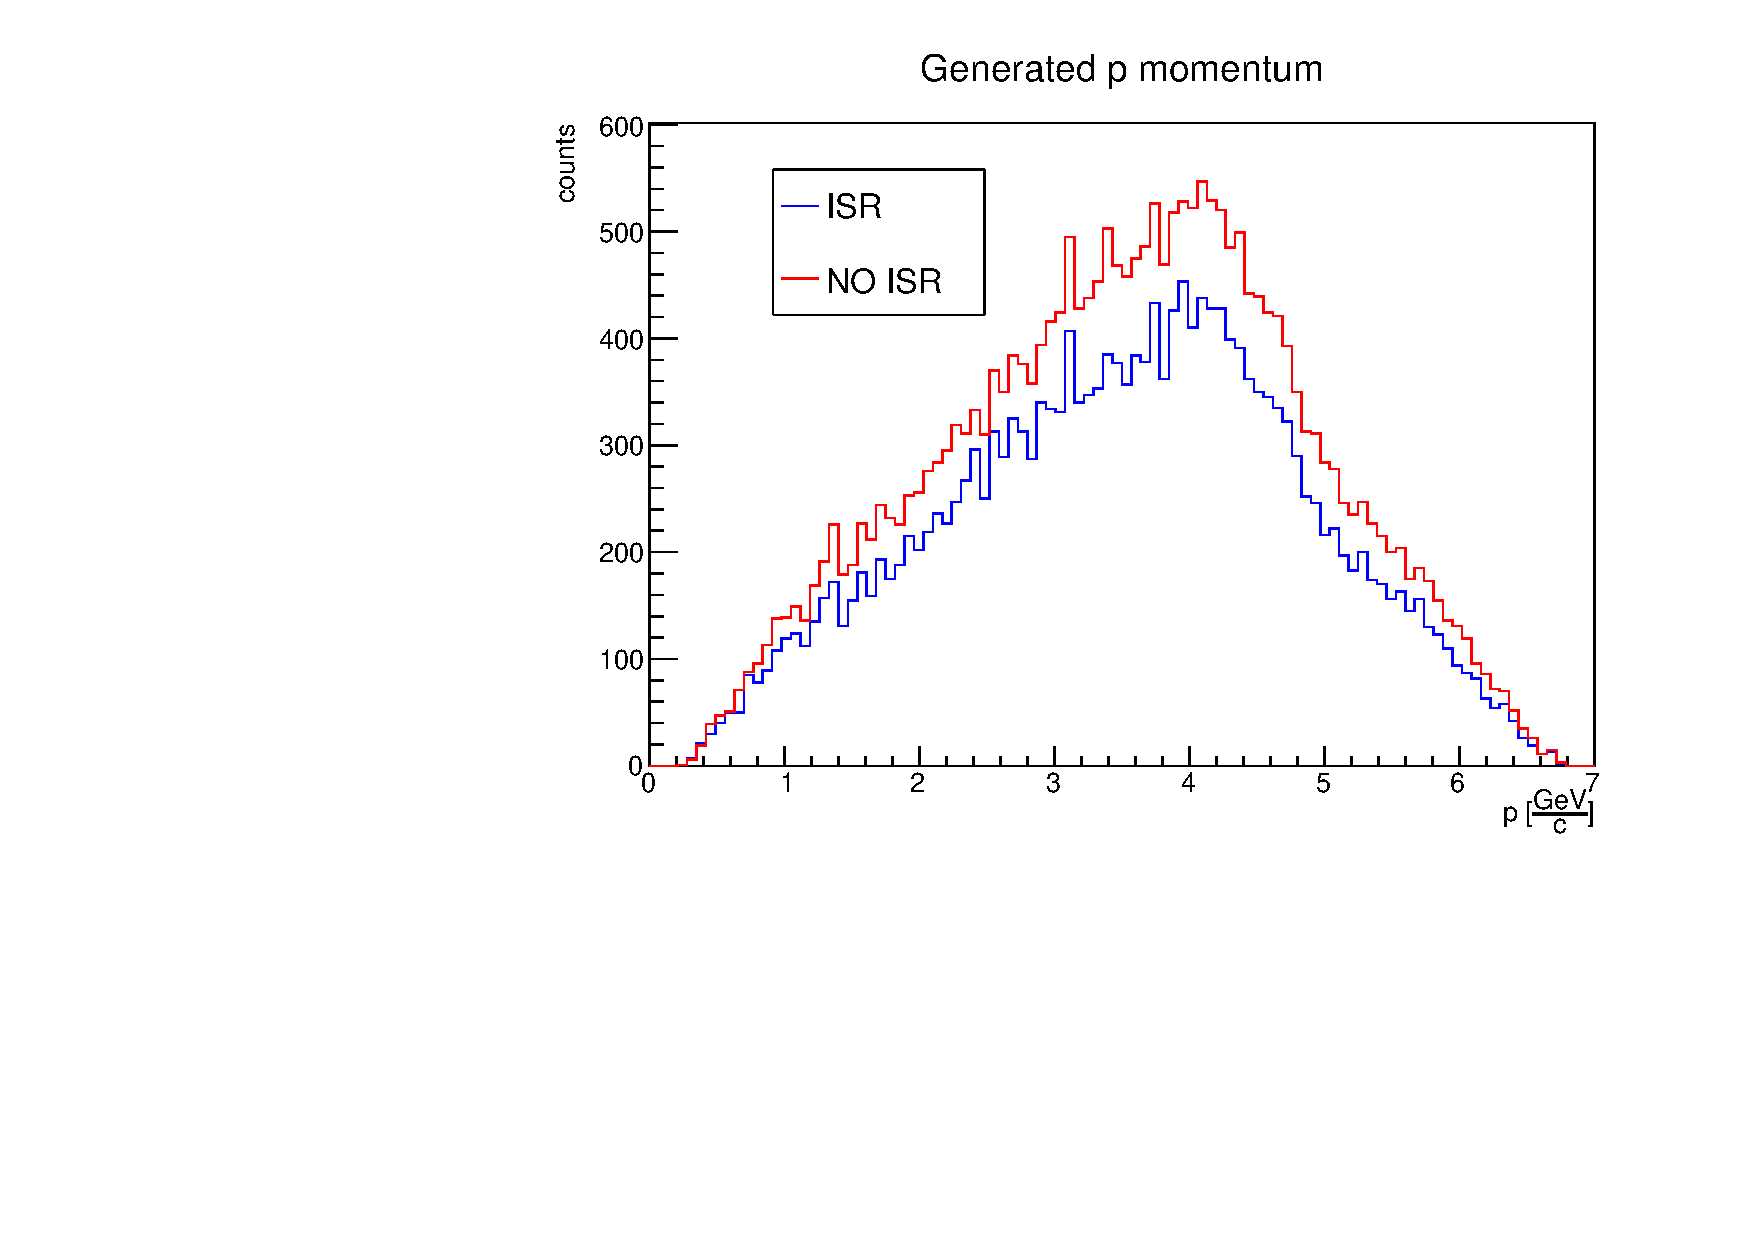
\includegraphics[width=0.49\textwidth]{nbar_MC/images/p_mcP.pdf}
    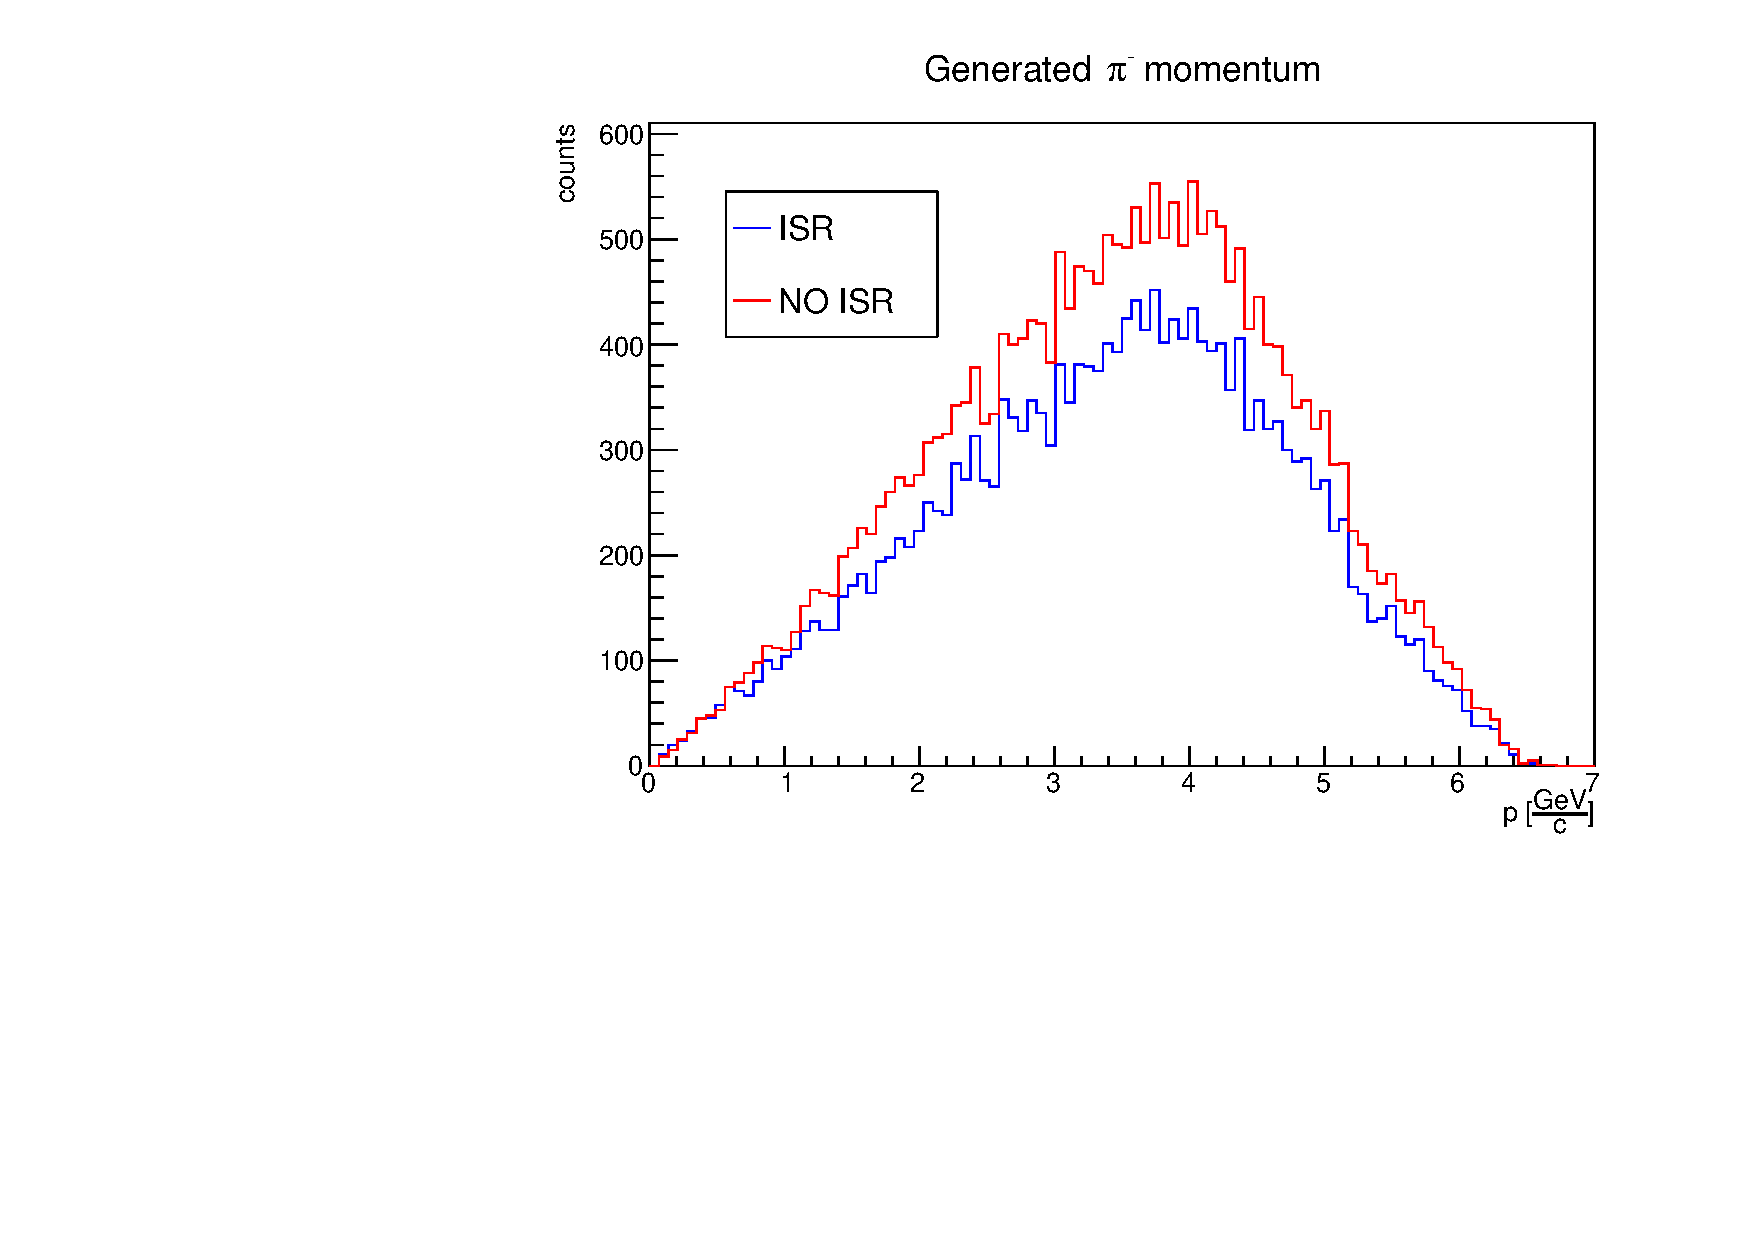
\includegraphics[width=0.49\textwidth]{nbar_MC/images/pi_mcP.pdf}
        \caption{Generated momentum distribution of proton and pion, in both ISR and NO ISR cases}
\end{figure}

Both distributions exhibit similar shapes, indicating a proper reconstruction of charged particles by the software.
$\\$
The reconstructed recoil momentum can be obtained in both ISR and NO ISR cases, as follows:

\begin{figure}[H]
    \centering
    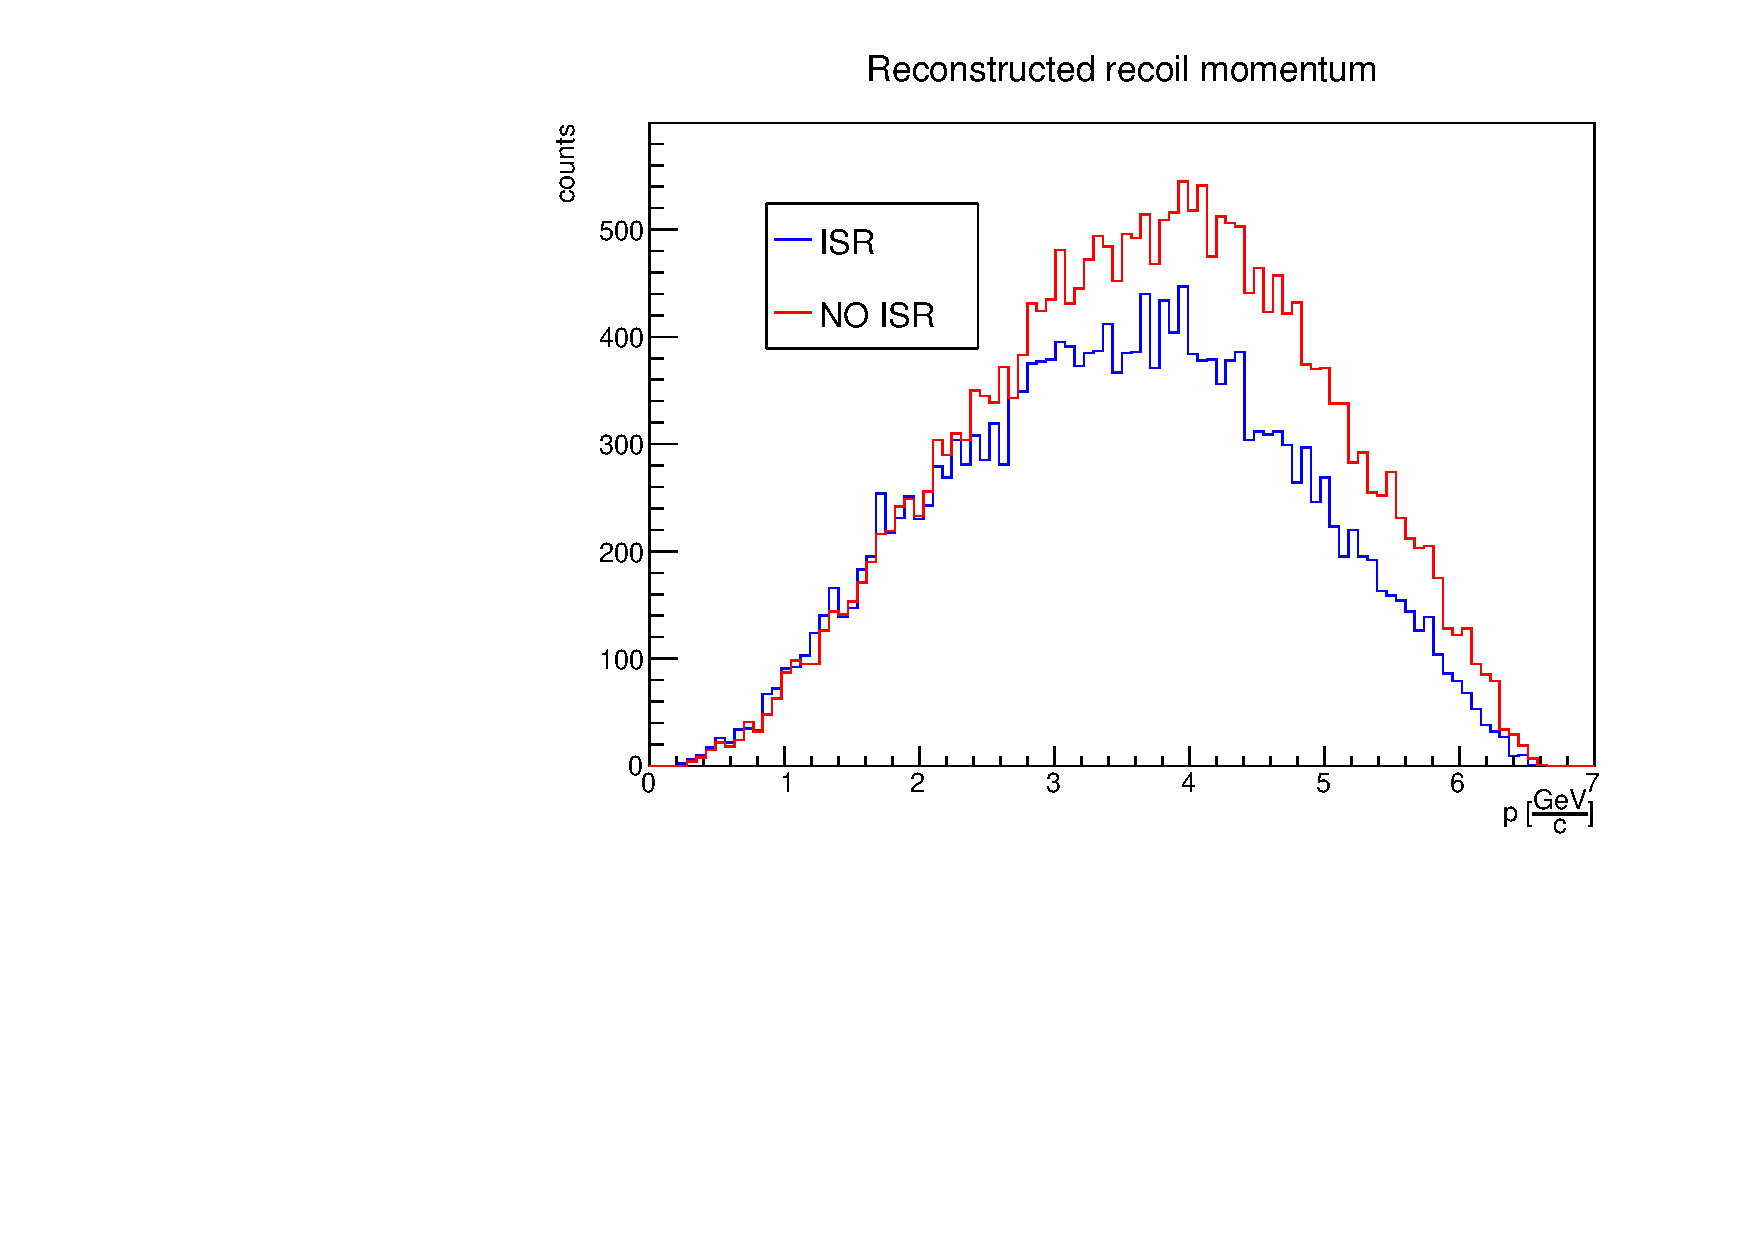
\includegraphics[width=0.70\textwidth]{nbar_MC/images/pRecoil.pdf}
    \caption{Reconstructed momentum distribution of the recoil system, in both ISR and NO ISR cases}
\end{figure}

Since the recoil system is well reconstructed through the recoil mass, it could be interesting to compare this distribution with that of $\bar{n}$, both from reconstruction and from generator. The latter is not affected by detector propagation and therefore it represents the $\bar{n}$ candidates generated momentum, free from misidentification and directly originating from the generator. The aforementioned $\bar{n}$ distributions are shown below:

\begin{figure}[H]
    \centering
    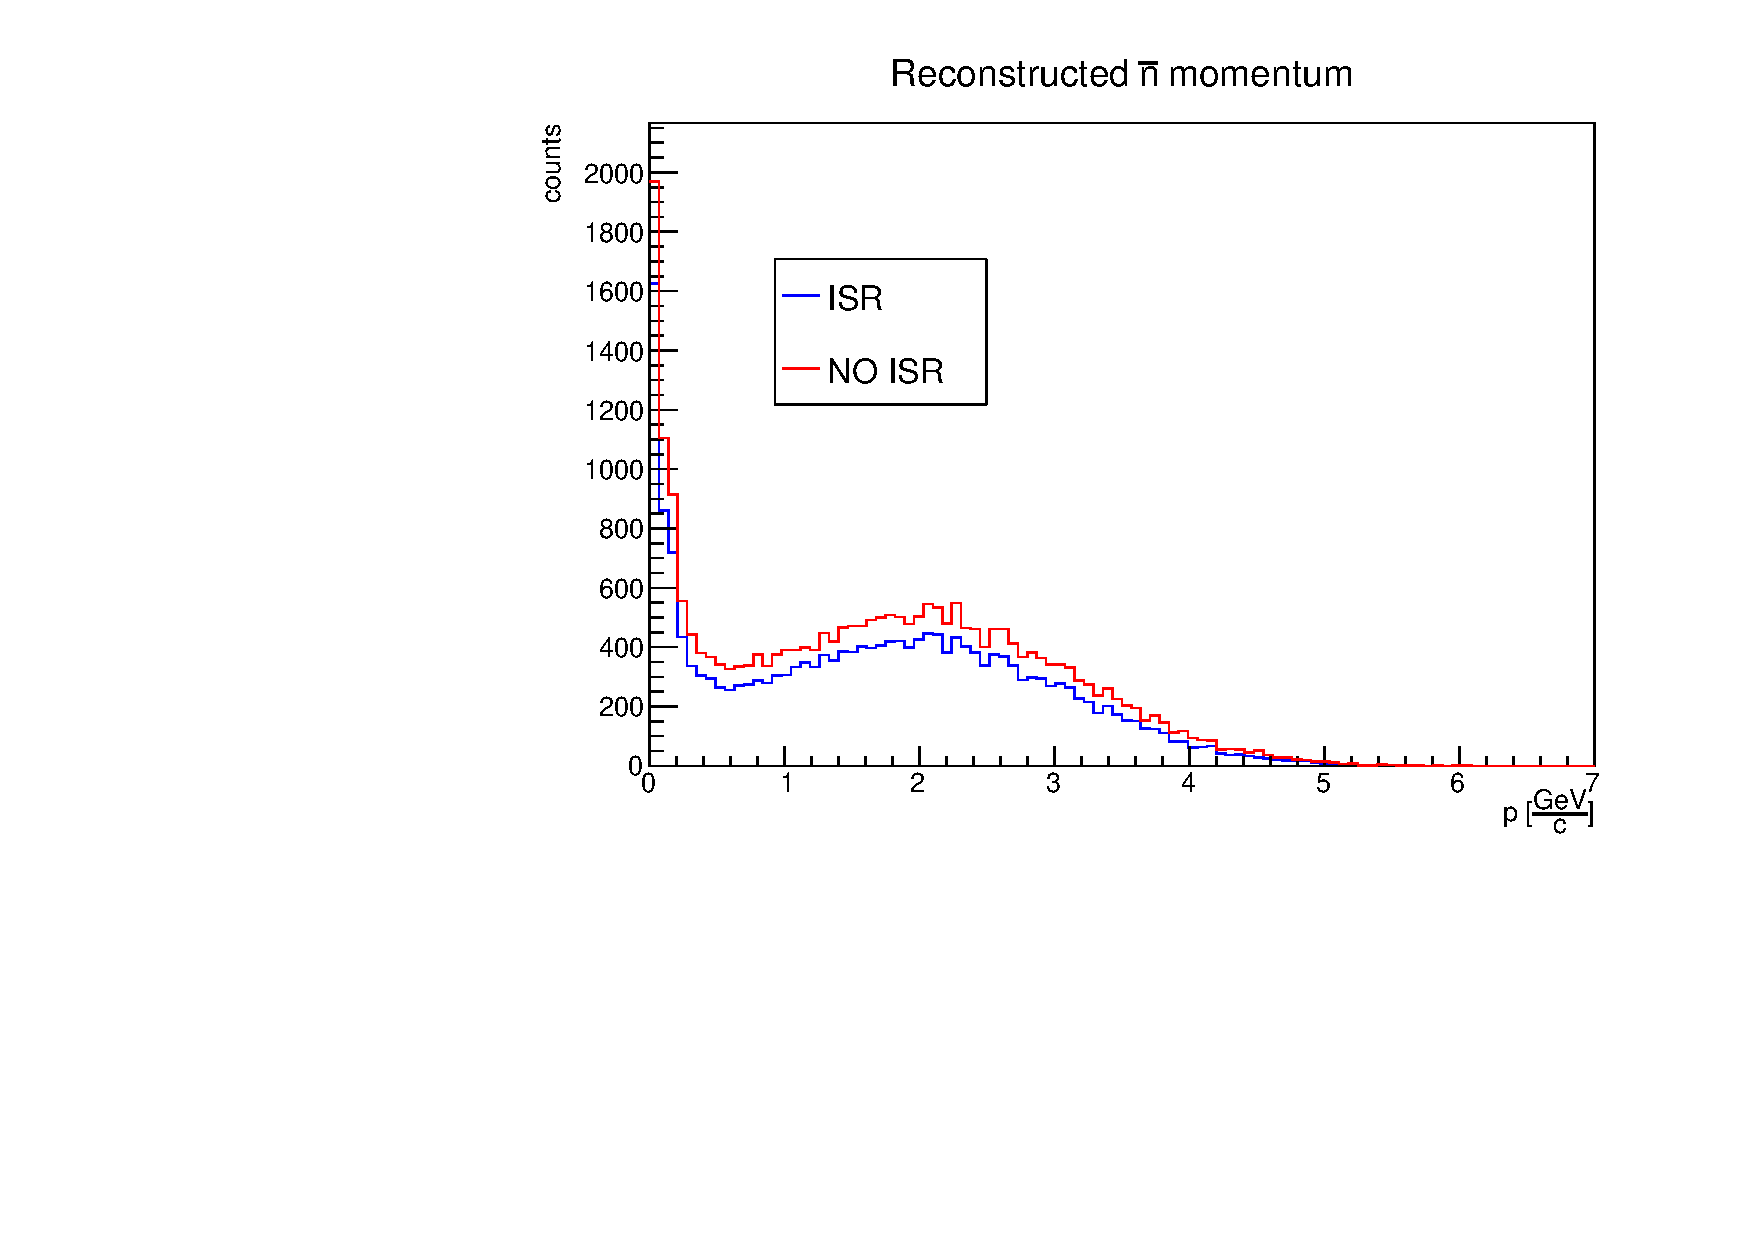
\includegraphics[width=0.49\textwidth]{nbar_MC/images/nbar_p.pdf}
    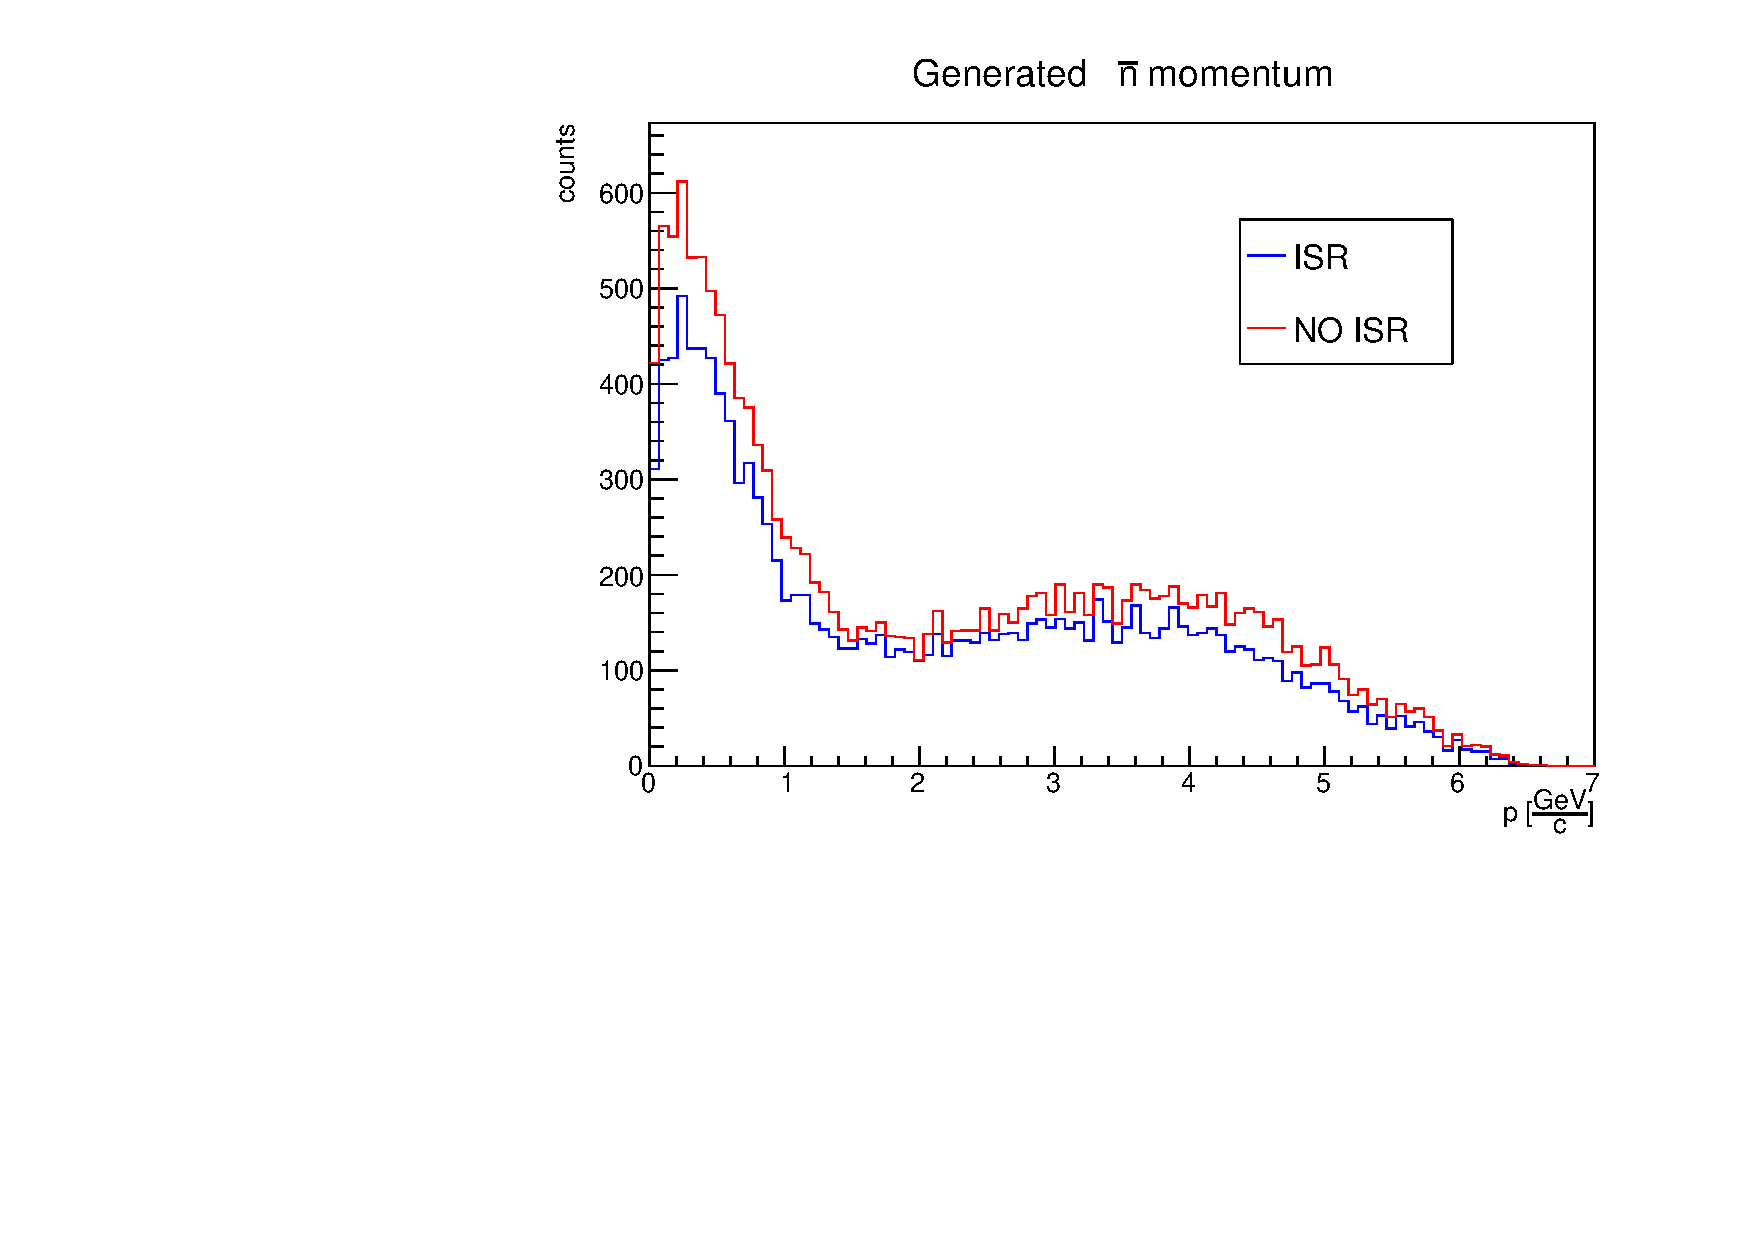
\includegraphics[width=0.49\textwidth]{nbar_MC/images/nbar_mcP.pdf}
    \caption{Reconstructed (left) and generated (right) momentum distribution of anti-neutron candidates, in both ISR and NO ISR cases}
\end{figure}

Notably, the reconstructed $\bar{n}$ momentum is systematically underestimated compared to the generator-level one, indicating missing energy within neutral clusters. This topic will be addressed in detail below through the momentum residuals.
$\\$
Both the reconstructed and generator-level distributions exhibit two structures, indicating two contributions within $\bar{n}$ candidate neutral clusters. To investigate this, the reconstructed recoil momentum is compared with the generator-level momentum of all $\bar{n}$ candidates, using MC truth matching. Since the $\bar{n}$ PDG code is \textbf{-2112}, the neutral clusters associated to $\bar{n}$ list can be matched to \textbf{true} (truth = 1) $\bar{n}$ particles, using Monte Carlo PDG $= -2112$, or to \textbf{false} (truth = 0) candidates with Monte Carlo PDG $\ne -2112$:

\begin{figure}[H]
    \centering
    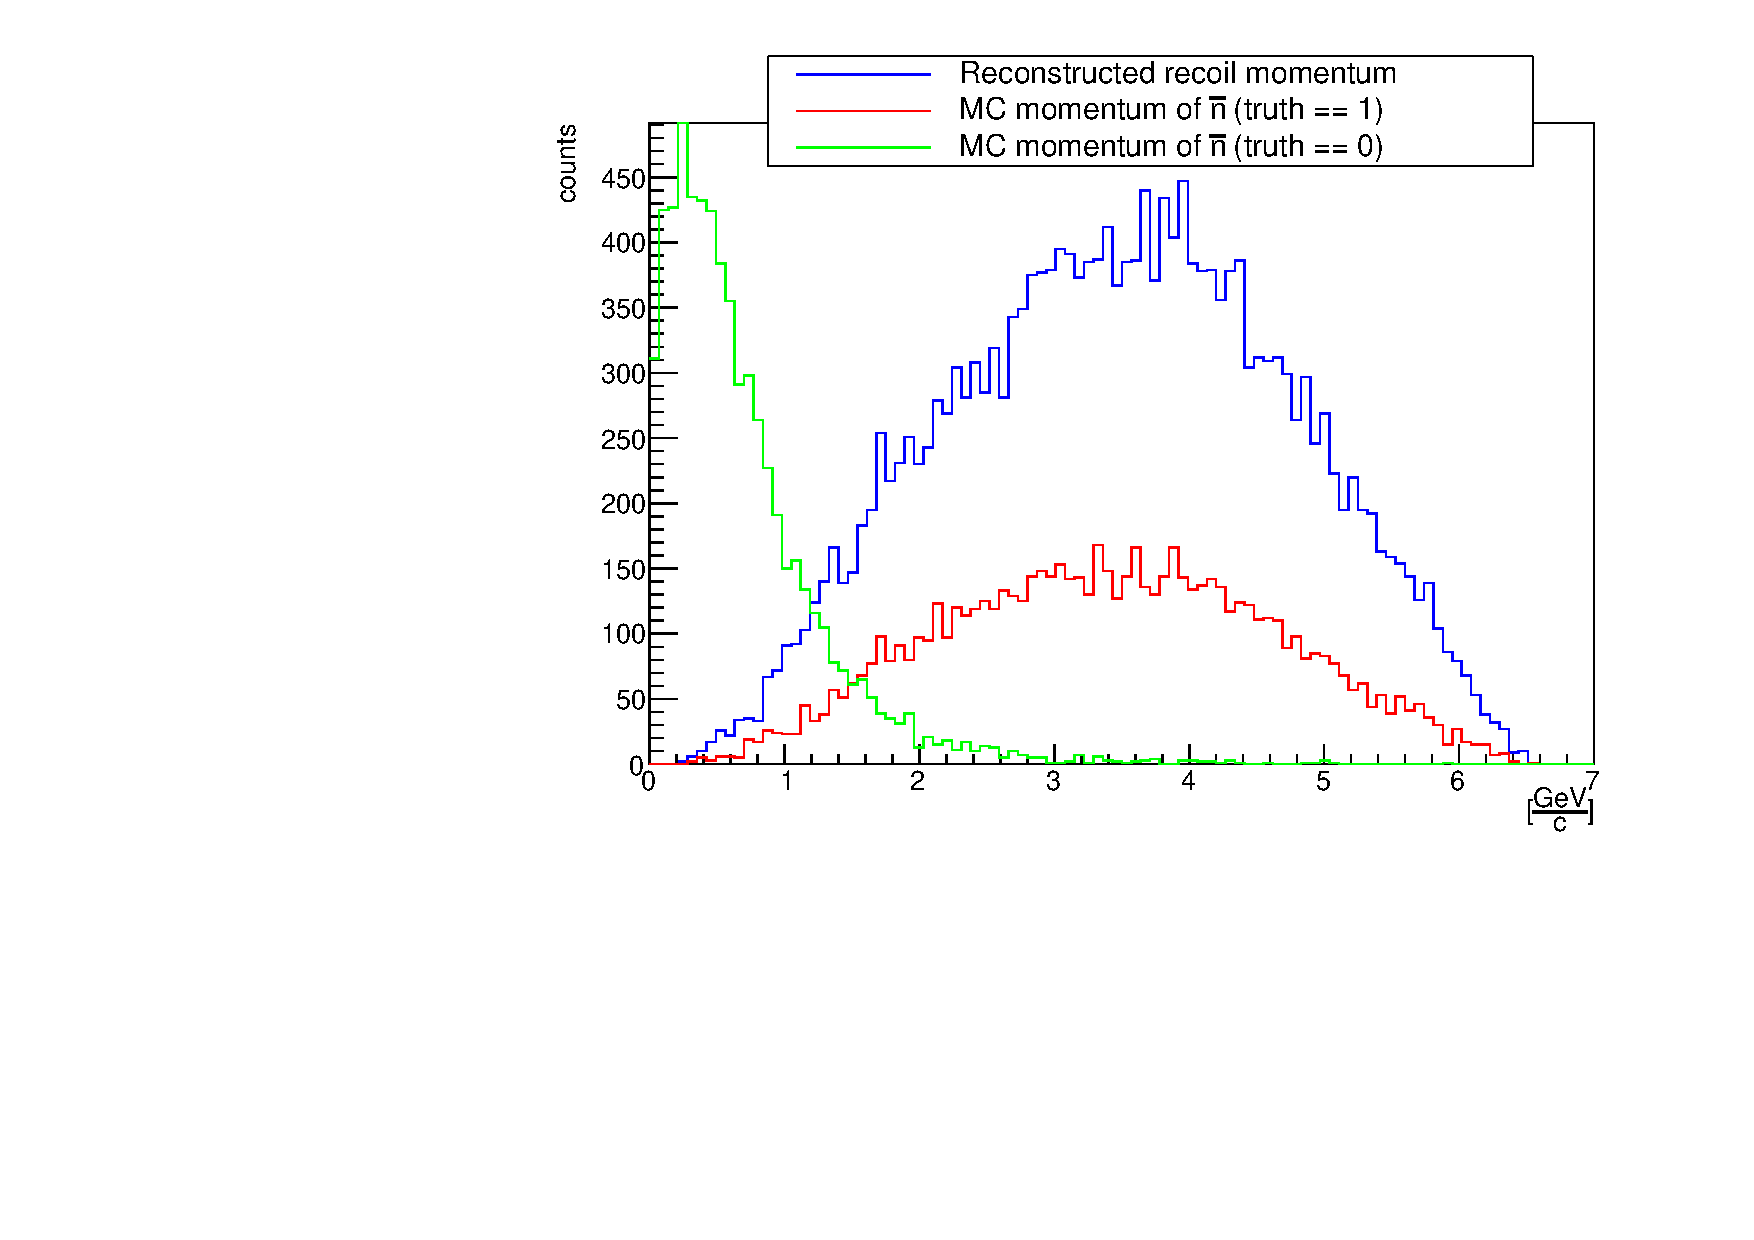
\includegraphics[width=0.49\textwidth]{nbar_MC/images/pRecoil_nmcP_isr.pdf}
    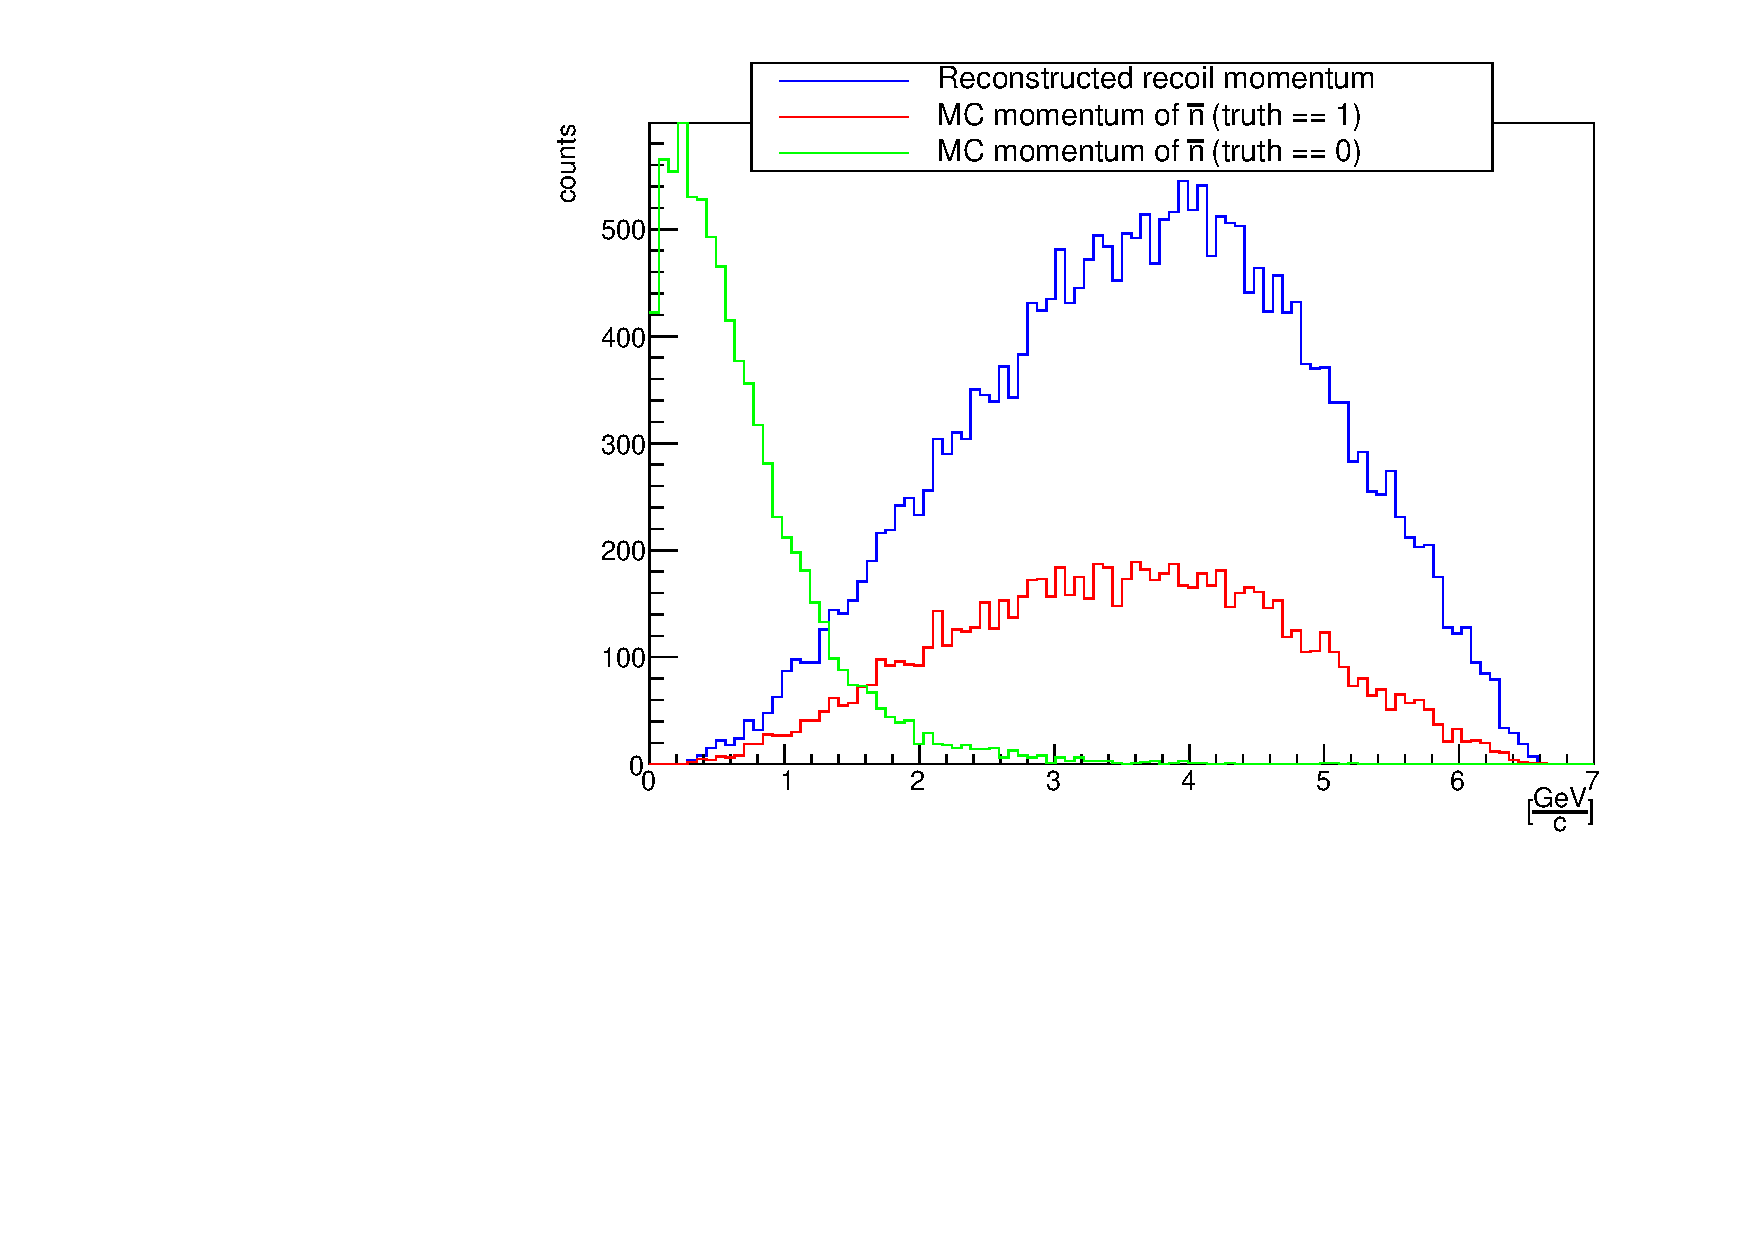
\includegraphics[width=0.49\textwidth]{nbar_MC/images/pRecoil_nmcP_nog.pdf}
    \caption{(left) Momentum contribution component in ISR case \\ (right) Momentum contribution component in NO ISR case}  
    \label{fig:pRecoil_nmcP} 
\end{figure}
    
As expected, the low-momentum structure corresponds to candidates not associated to $\bar{n}$ by the Monte Carlo truth, exhibiting significant deviation from the recoil momentum. This is likely due to cluster split-off and/or pre-showering effects as will be discussed later. Furthermore, the {\color{red} red distribution} is include within the {\color{blue} blue one}, suggesting that several anti-neutron are missing after the reconstruction. All these aspects will be discussed in the next section through analysis of $\bar{n}$ relatives (ancestors).      
$\\$
To compare the reconstructed recoil with the Monte Carlo matched $\bar{n}$ (truth = 1), it is useful to analyze their linear correlation coefficient $\rho$, recalling that:
\begin{center}
$\rho_{x,y} = \frac{cov[x,y]}{\sigma_x \sigma_y} $ \hspace{0.5cm} where $cov[x,y] = E[xy] - E[x]E[y]$
\end{center}

Therefore, the correlations in $\theta$, for both the reconstructed and the generated case, are shown below:

\begin{figure}[H]
    \centering
     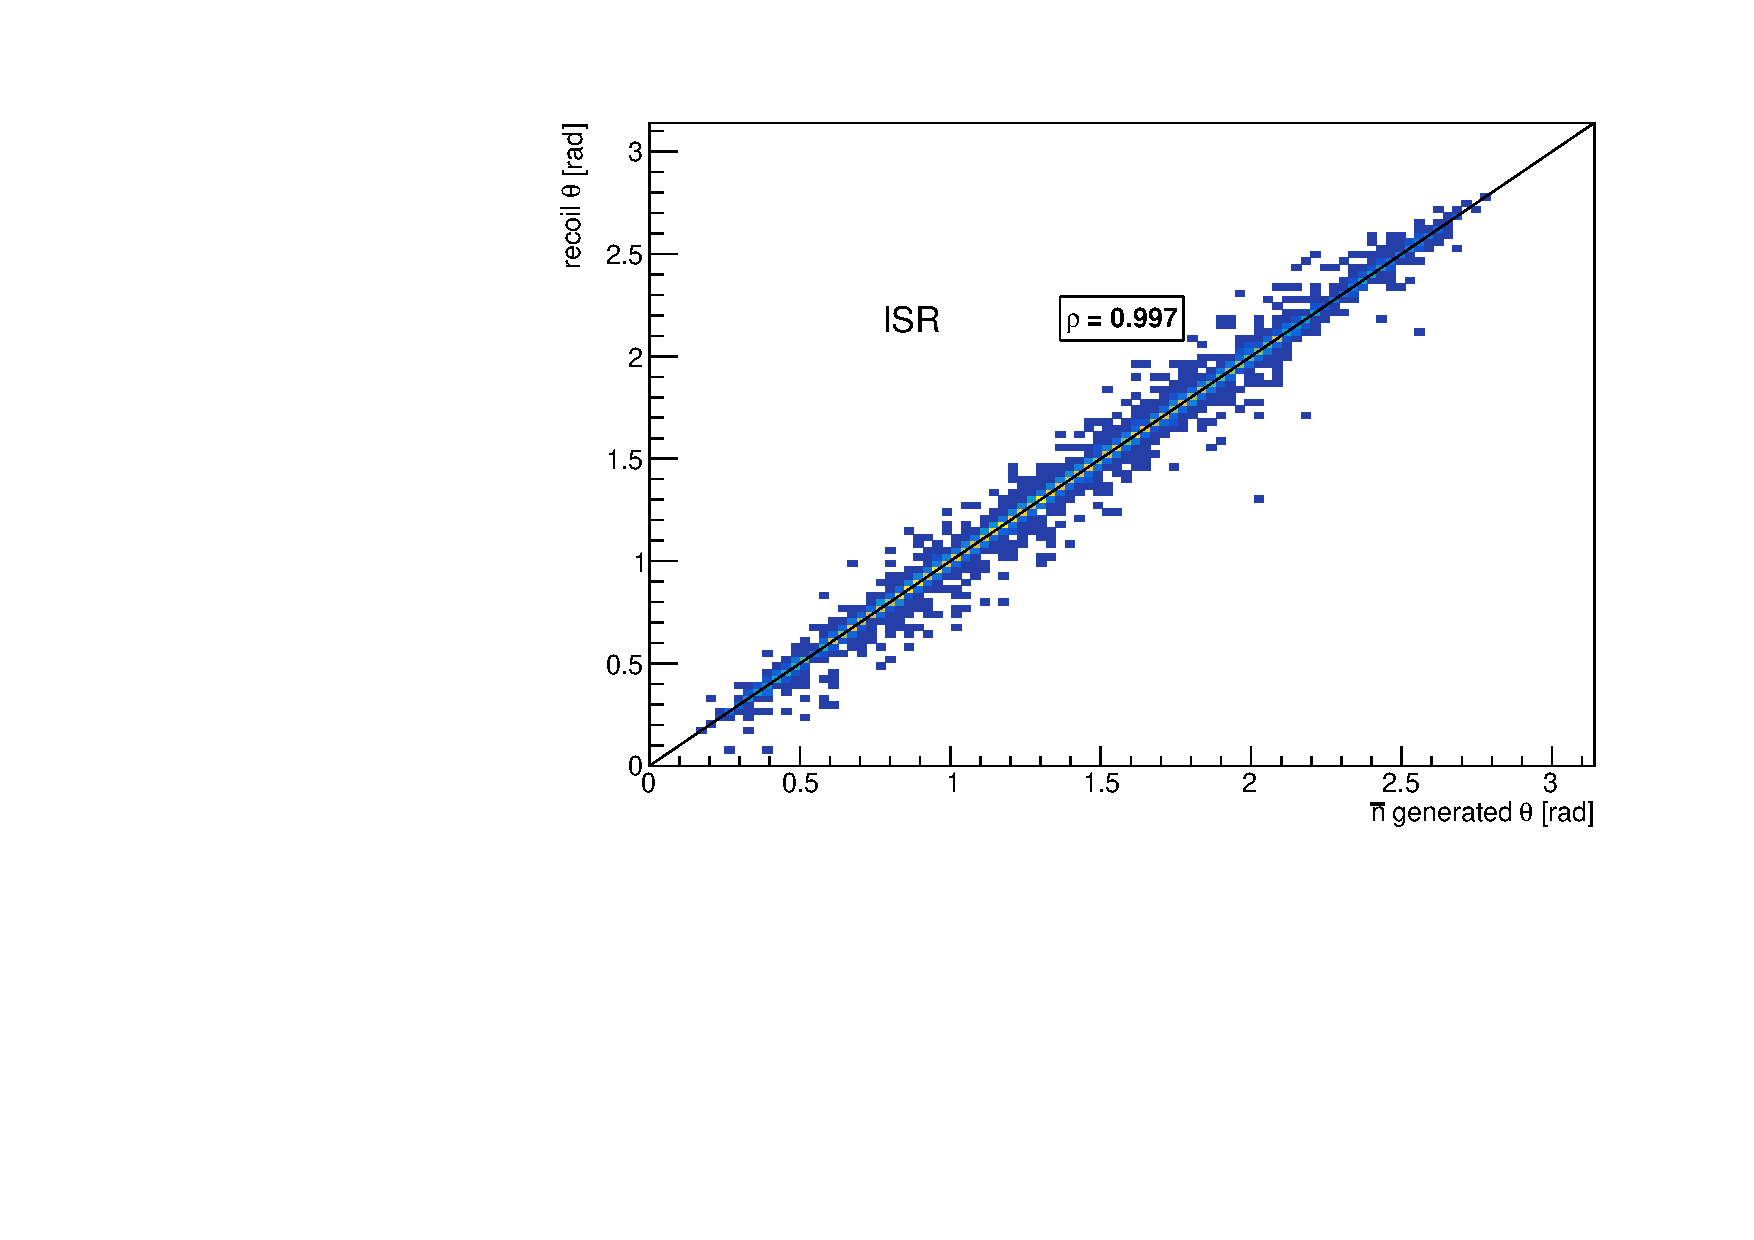
\includegraphics[width=0.49\textwidth]{nbar_MC/images/gen_mc_theta_corr_isr.pdf}
     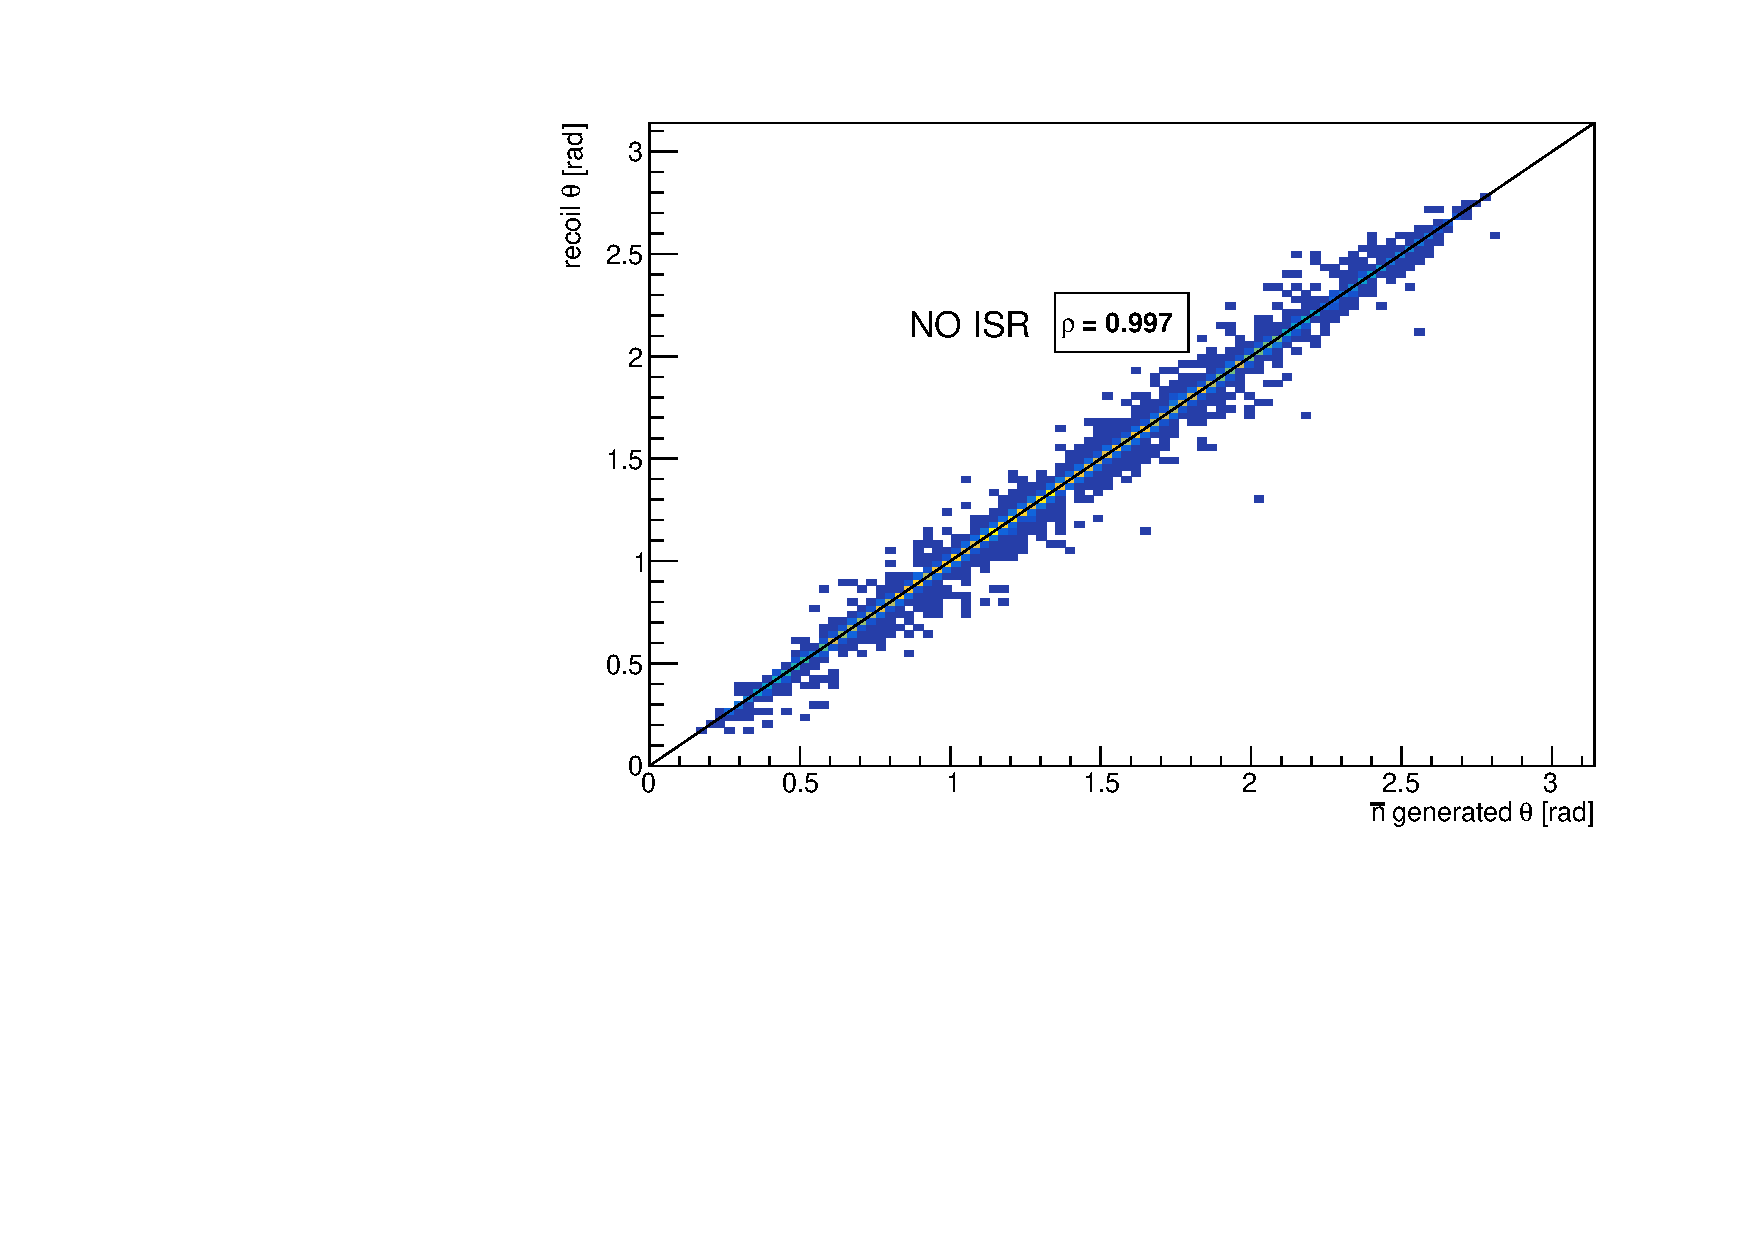
\includegraphics[width=0.49\textwidth]{nbar_MC/images/gen_mc_theta_corr_nog.pdf}
     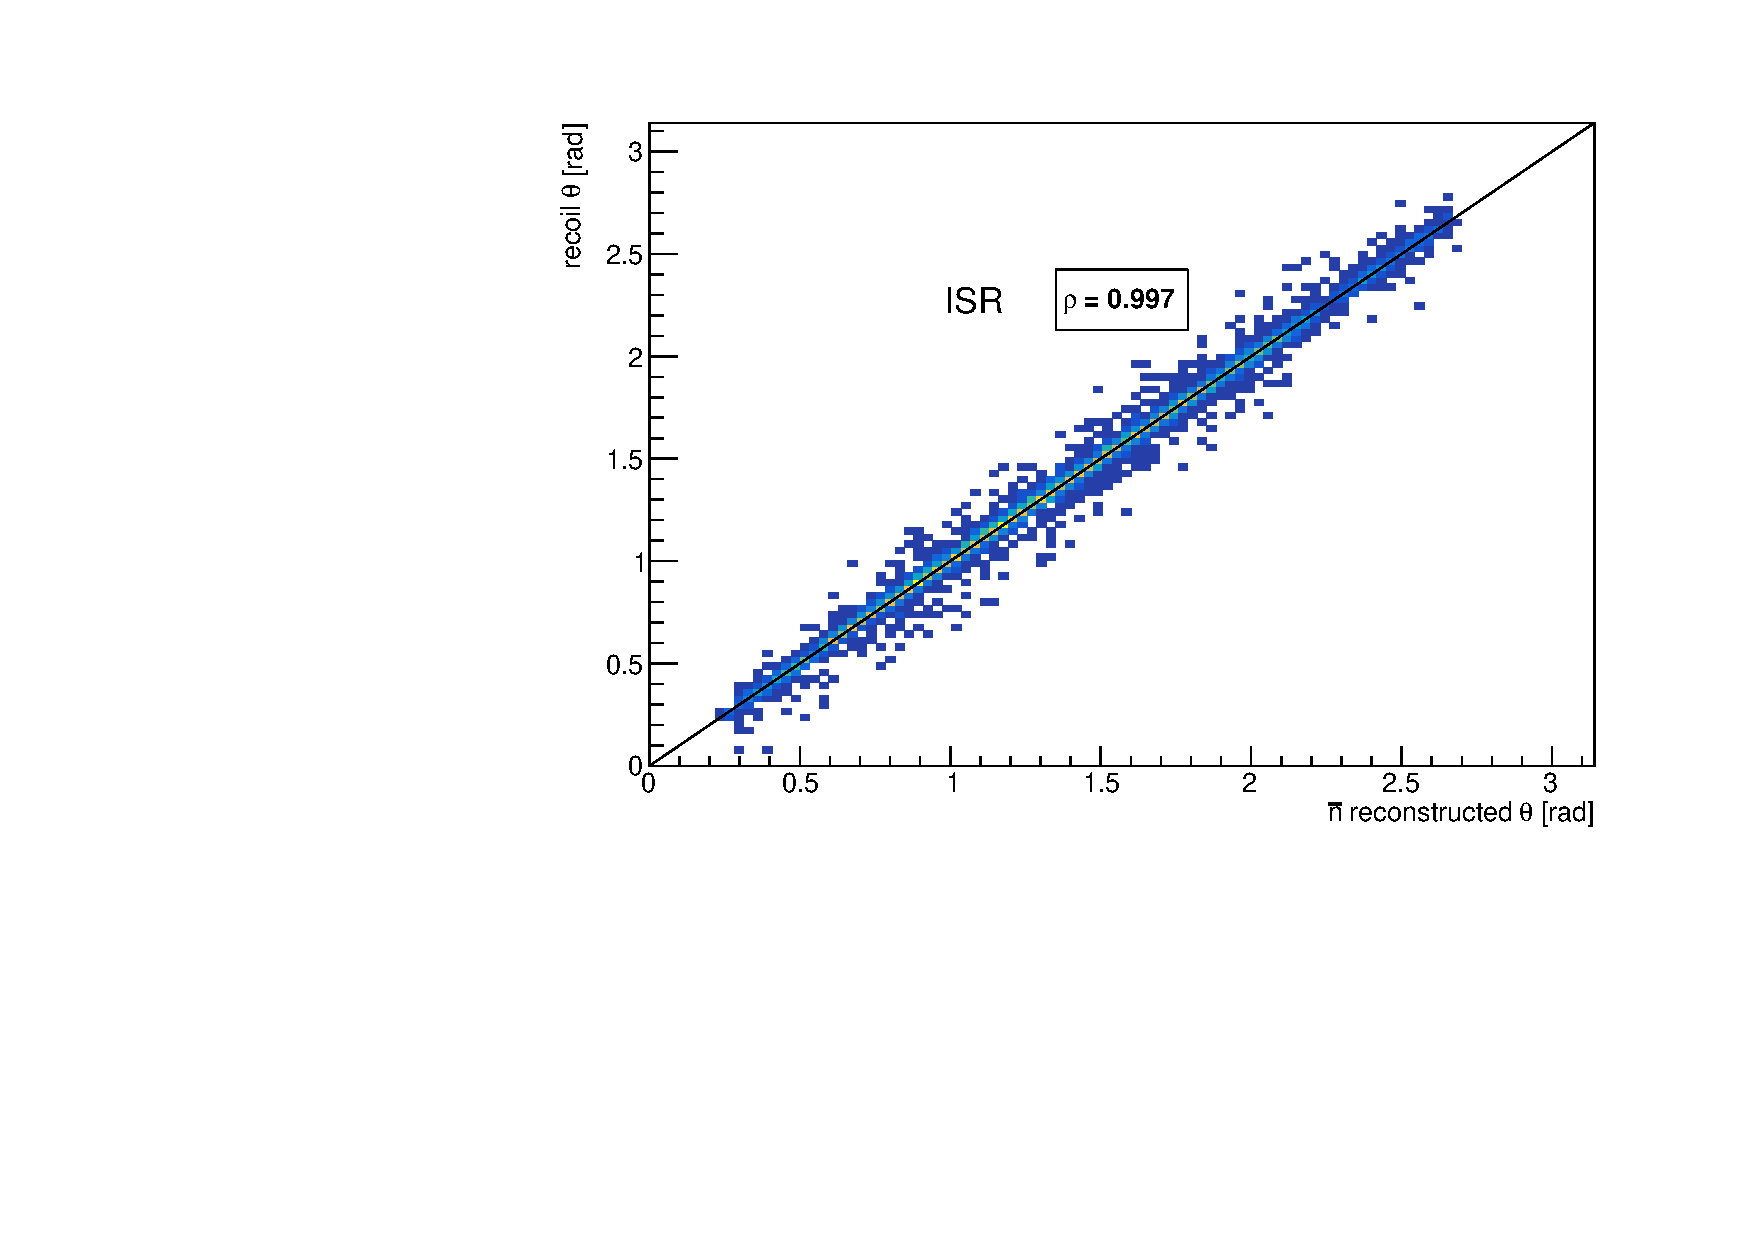
\includegraphics[width=0.49\textwidth]{nbar_MC/images/gen_rec_theta_corr_isr.pdf}
     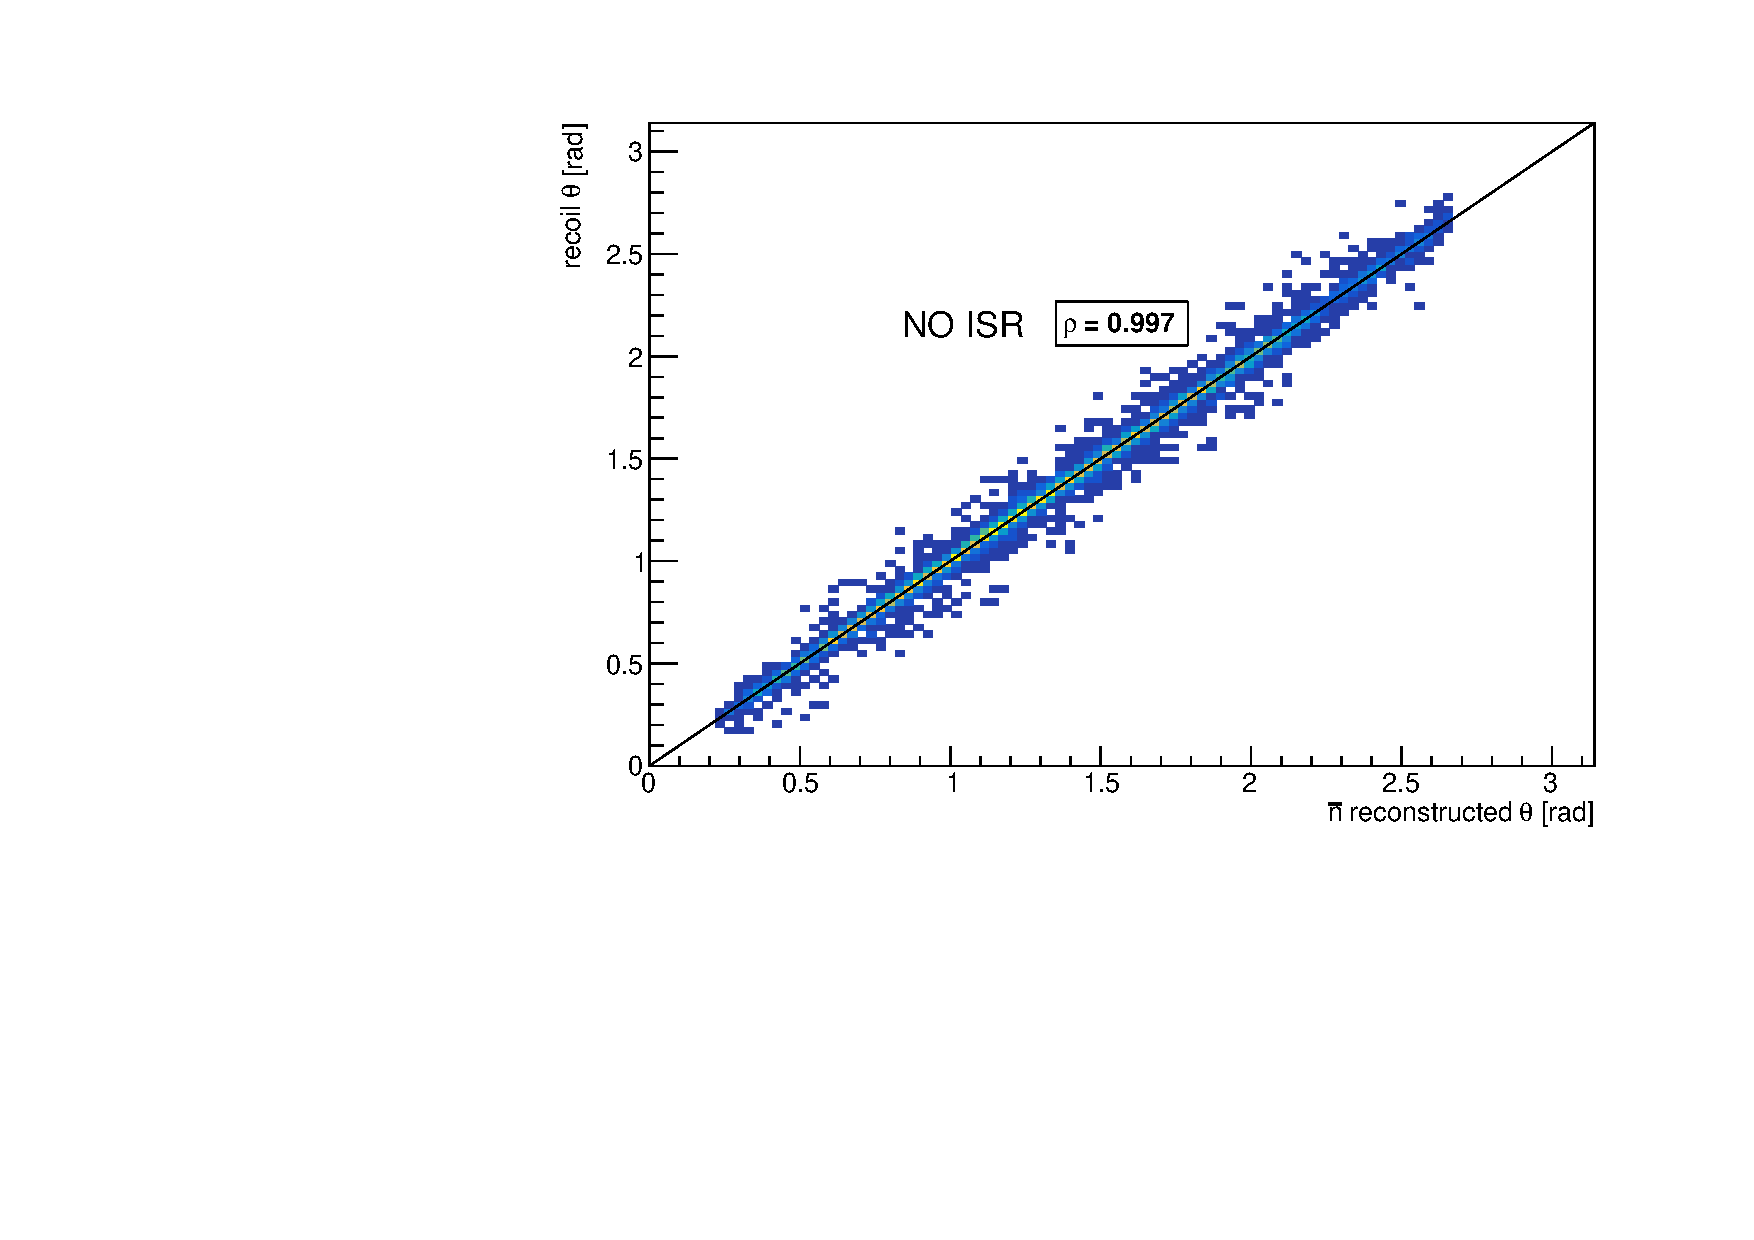
\includegraphics[width=0.49\textwidth]{nbar_MC/images/gen_rec_theta_corr_nog.pdf}
      \caption{$\theta$ correlation distribution between recoil system and anti-neutron candidate, in both reconstructed and generated case. Linear correlation coefficient $\rho$ truncated to three decimal places}
\end{figure}

A good correlation can be highlighted between the two distributions in both reconstructed and generator-level cases, indicating that the the anti-neutron $\theta$ direction is properly described.
$\\$
The same comparison can be addressed for the momentum, remembering that it is obtained starting from the energy of the cluster as follow:
 \begin{center}
$p_{rec}^2 = E_{ECL}^2 - m_{\bar{n}}^2$
\end{center}

The obtained conjugate distributions are shown below:
\begin{figure}[H]
    \centering
     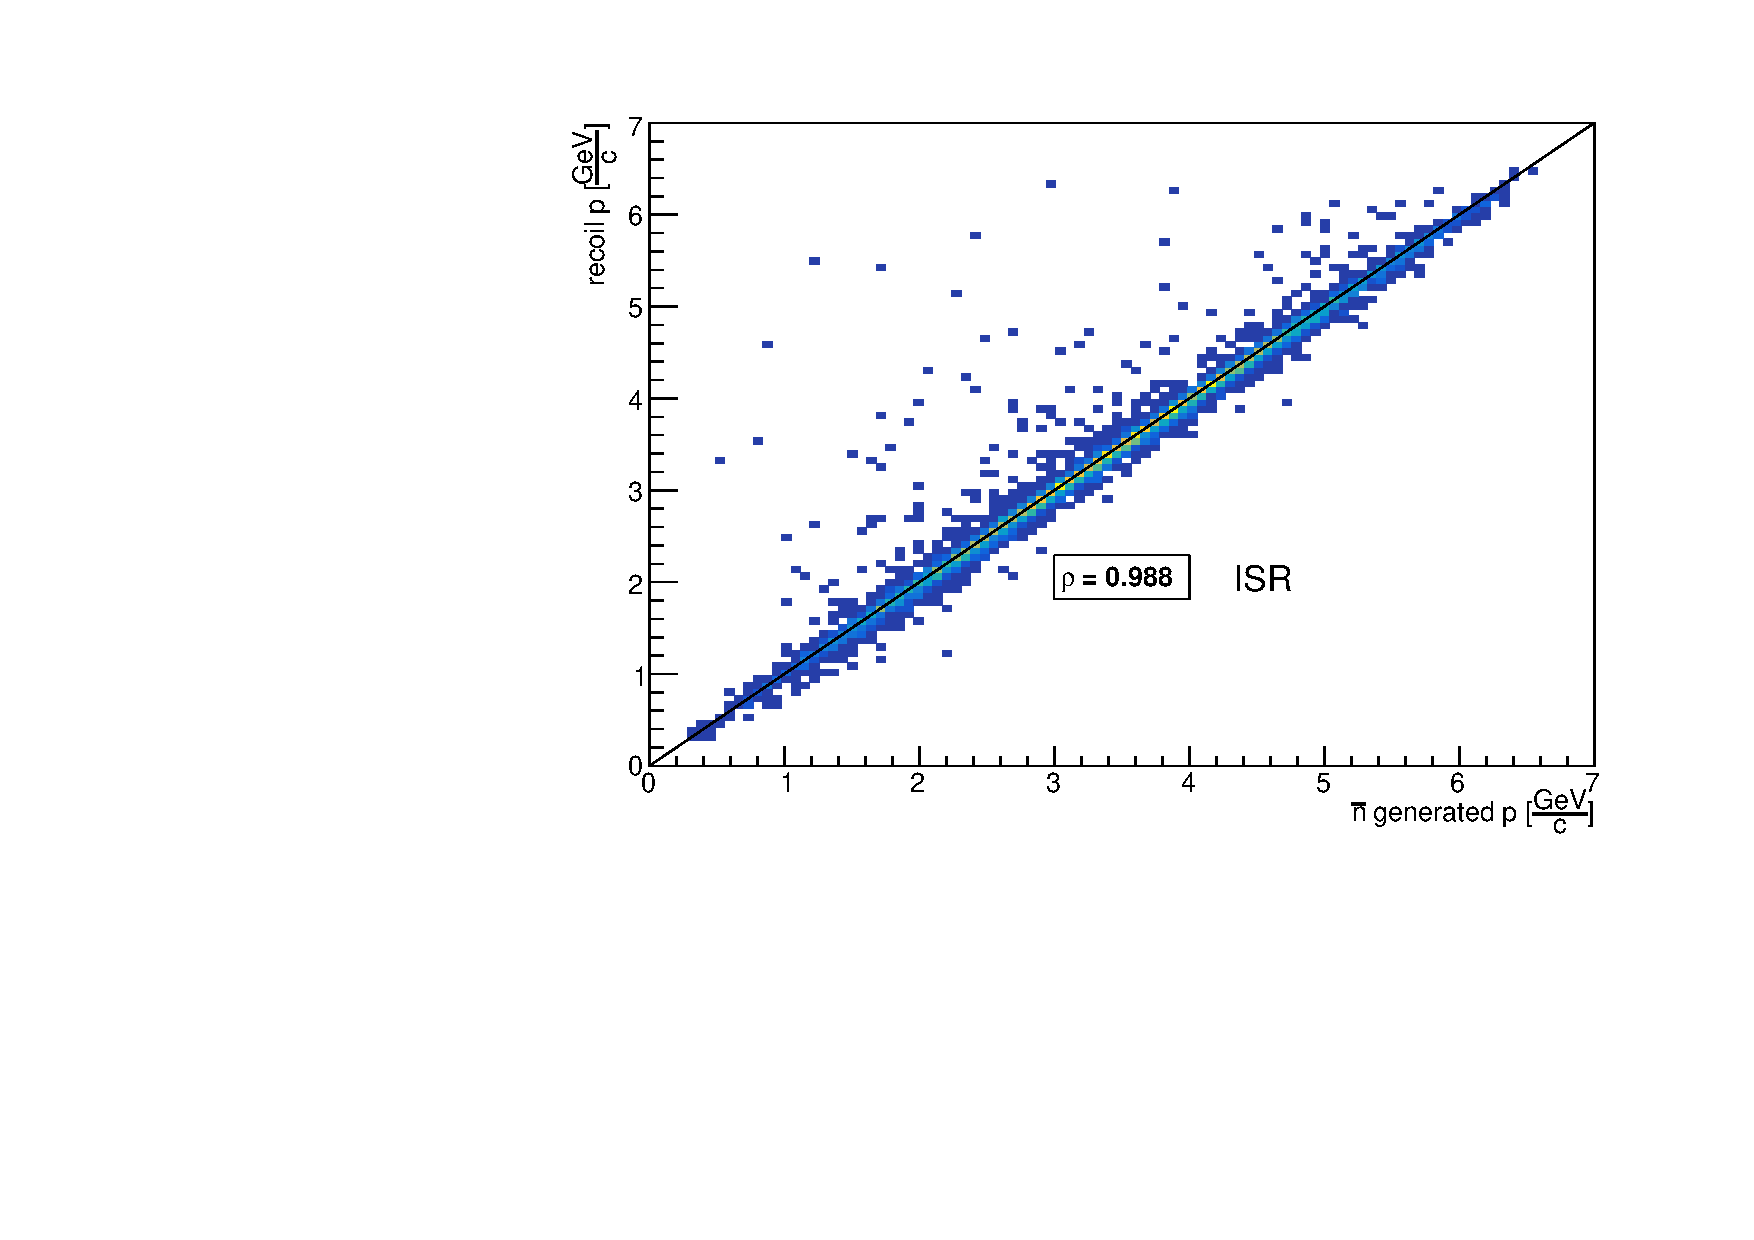
\includegraphics[width=0.49\textwidth]{nbar_MC/images/gen_mc_p_corr_isr.pdf}
     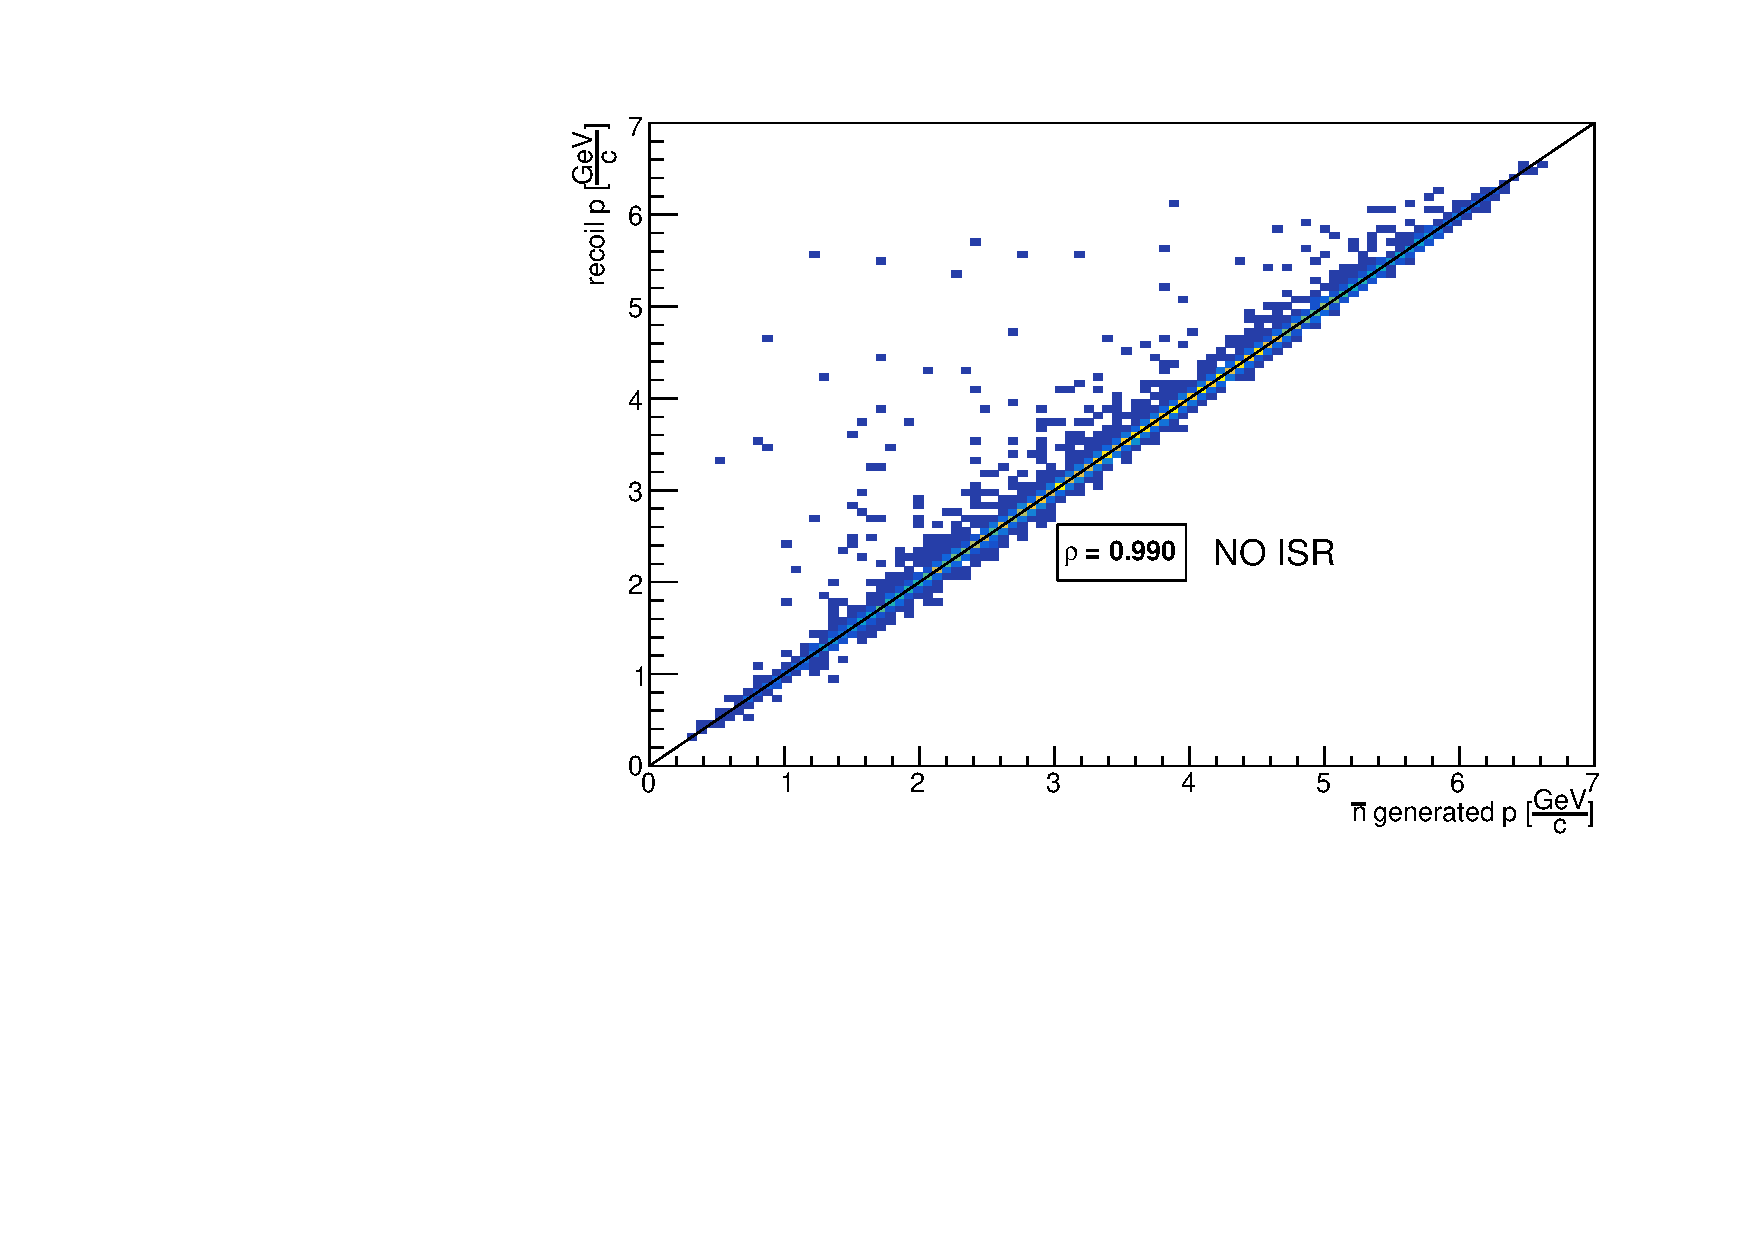
\includegraphics[width=0.49\textwidth]{nbar_MC/images/gen_mc_p_corr_nog.pdf}
     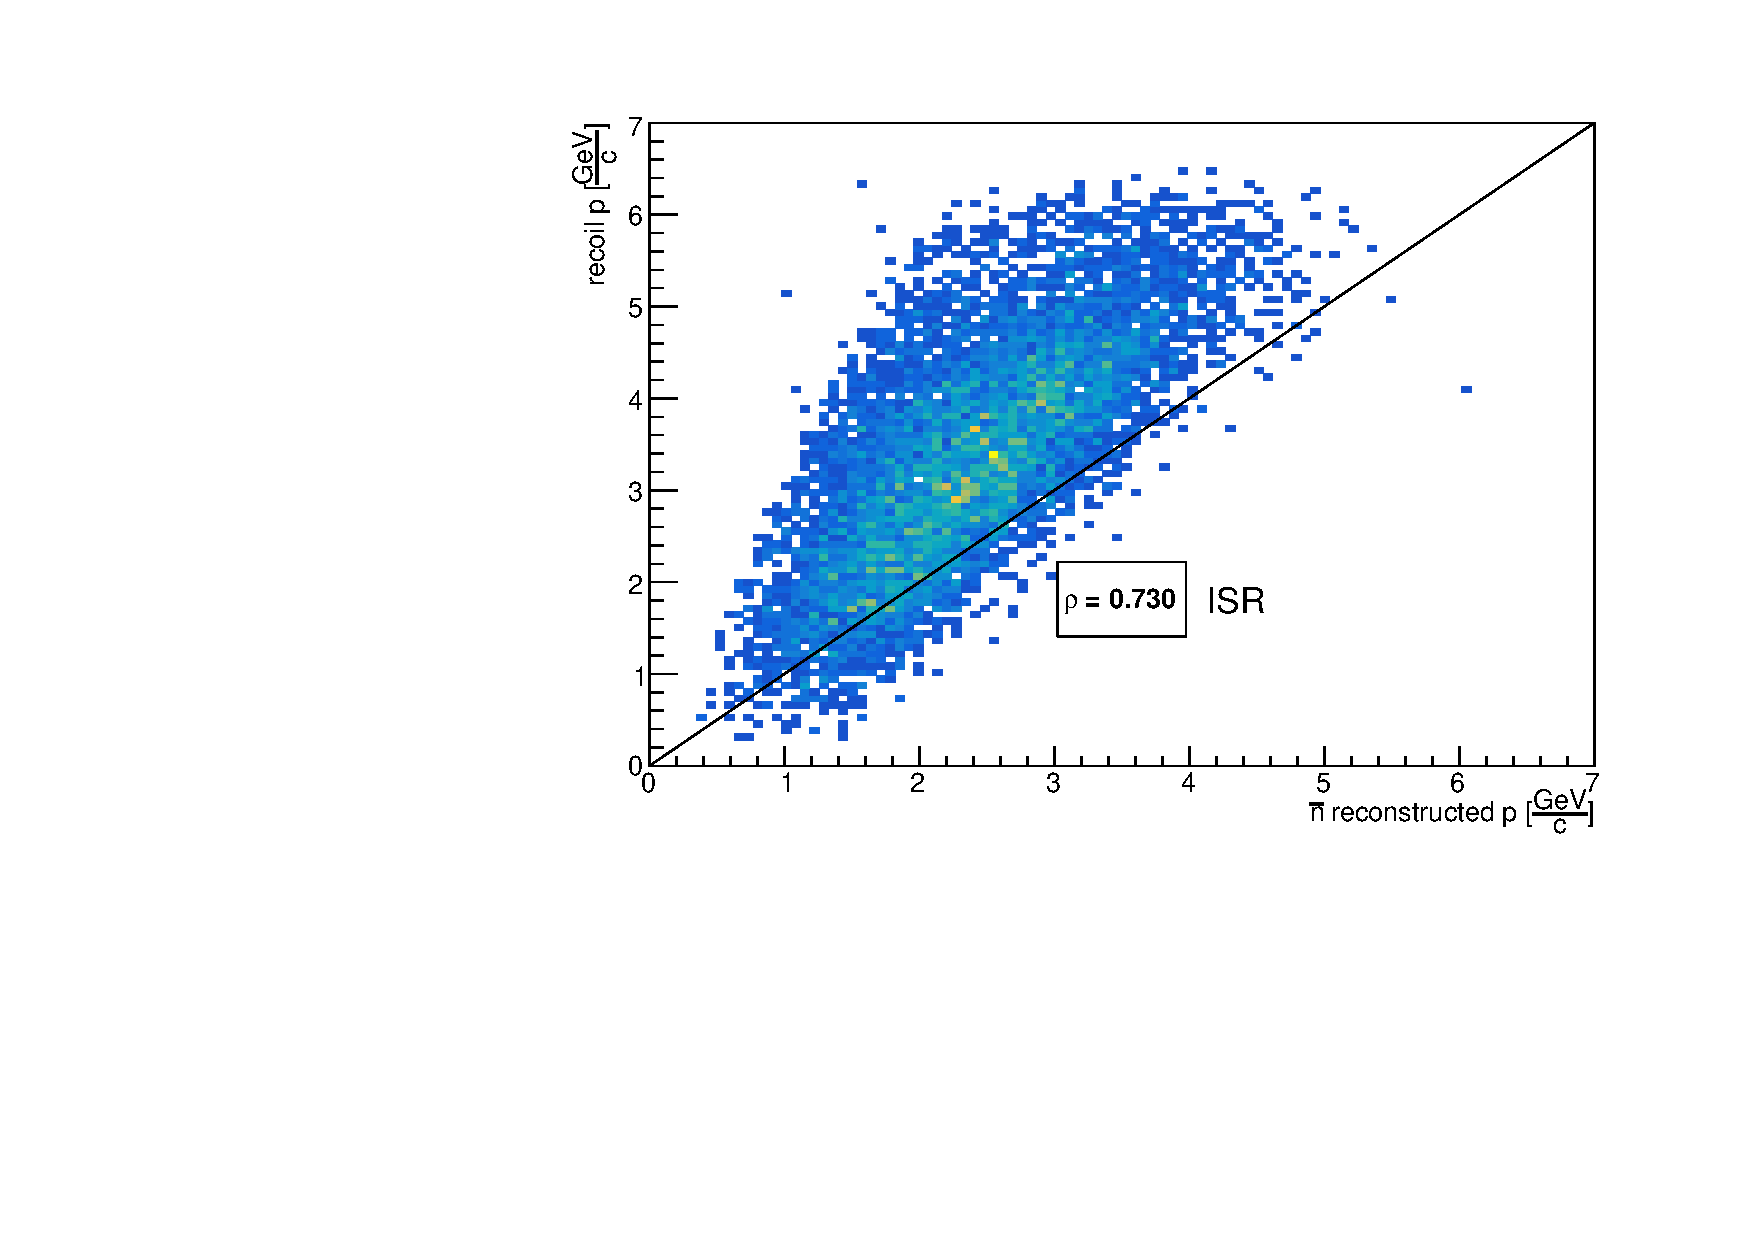
\includegraphics[width=0.49\textwidth]{nbar_MC/images/gen_rec_p_corr_isr.pdf}
     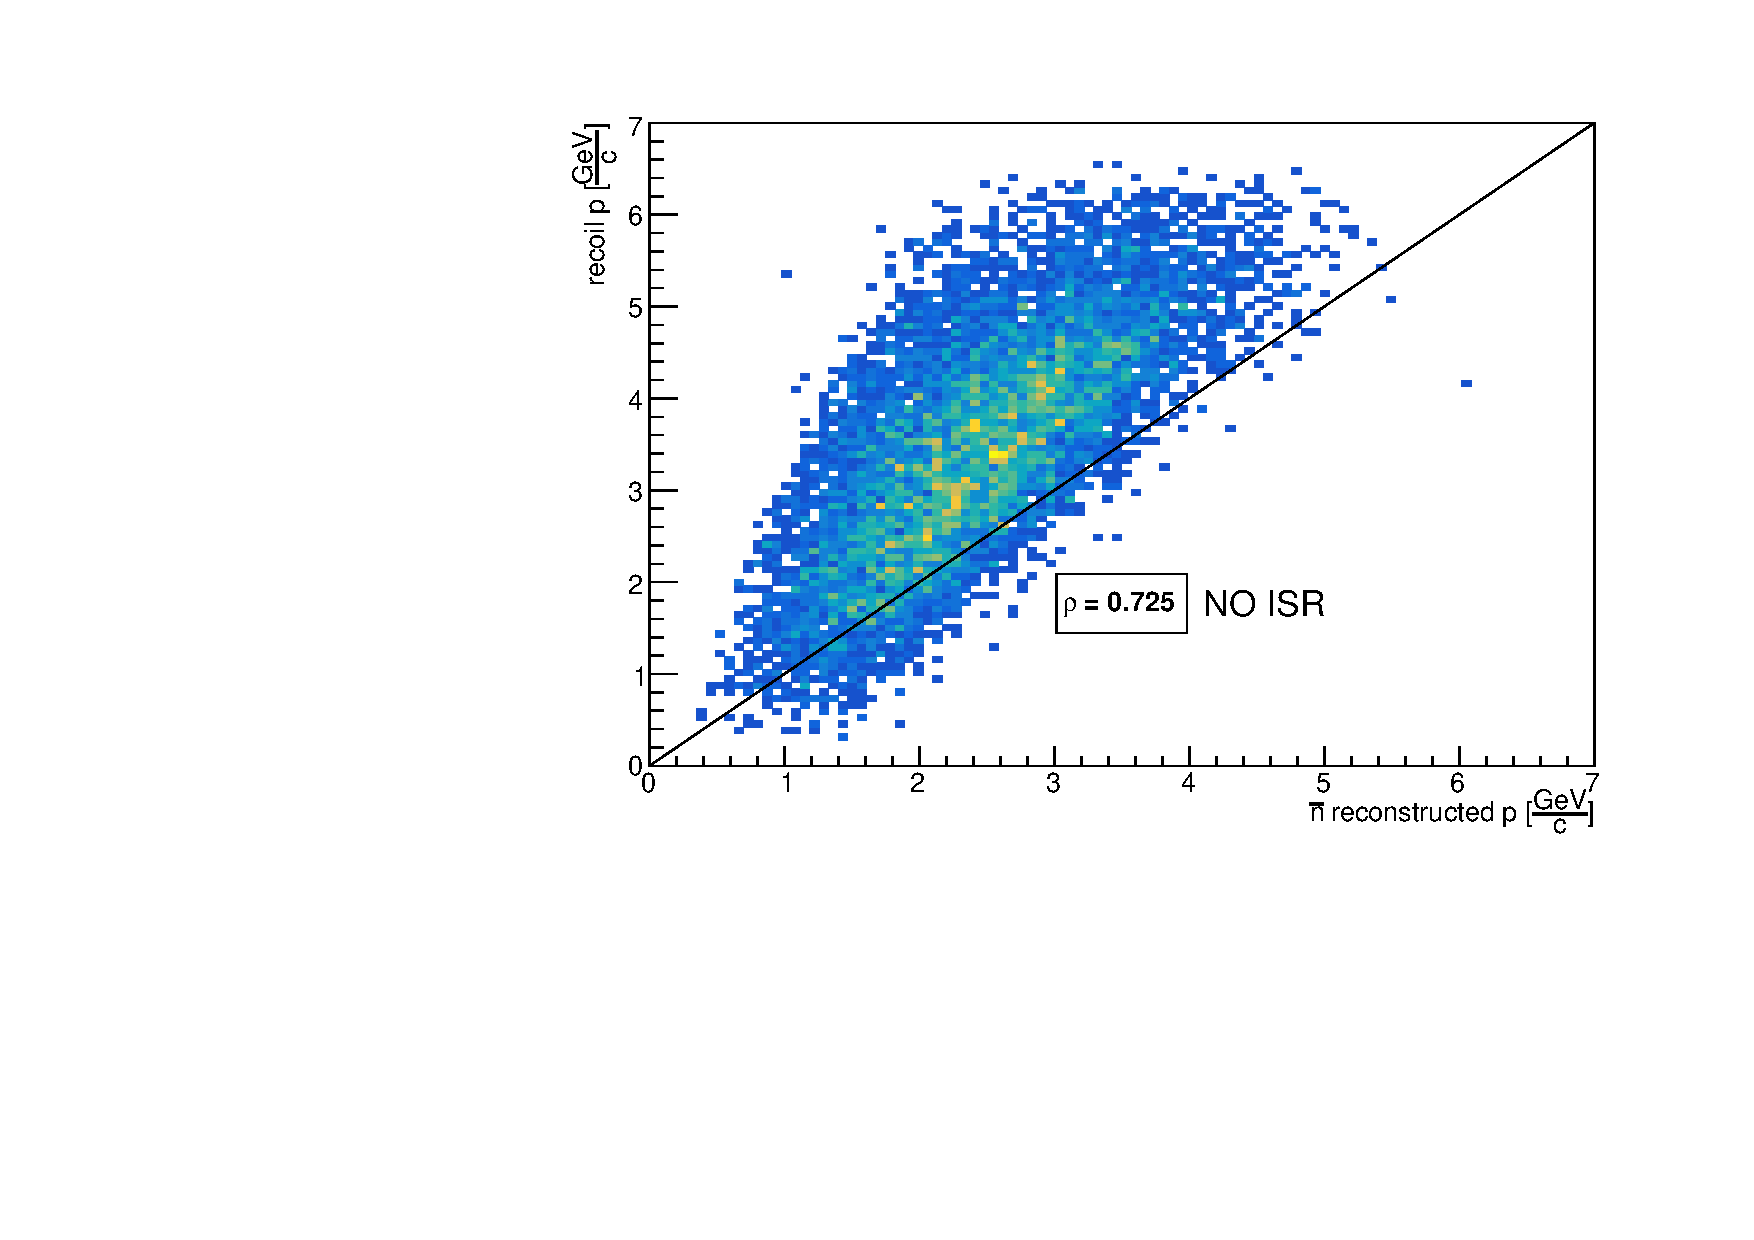
\includegraphics[width=0.49\textwidth]{nbar_MC/images/gen_rec_p_corr_nog.pdf}
      \caption{Momentum correlation distribution between recoil system and anti-neutron candidate, in both reconstructed and generated case. Linear correlation coefficient $\rho$ truncated to three decimal places}
      \label{fig:pRecoil-nP}
\end{figure}

A good correlation can be observed between the reconstructed recoil momentum and the generated $\bar{n}$ one, confirming how the first is properly describing the $\bar{n}$ kinematic.
$\\$
However, a poor resolution is observed in reconstructed $\bar{n}$ momentum, in both ISR and NO ISR cases, presenting an underestimation of the reconstructed $\bar{n}$ momentum as well. In order to directly study it, the momentum residual can be analyzed:
\begin{figure}[H]
    \centering
     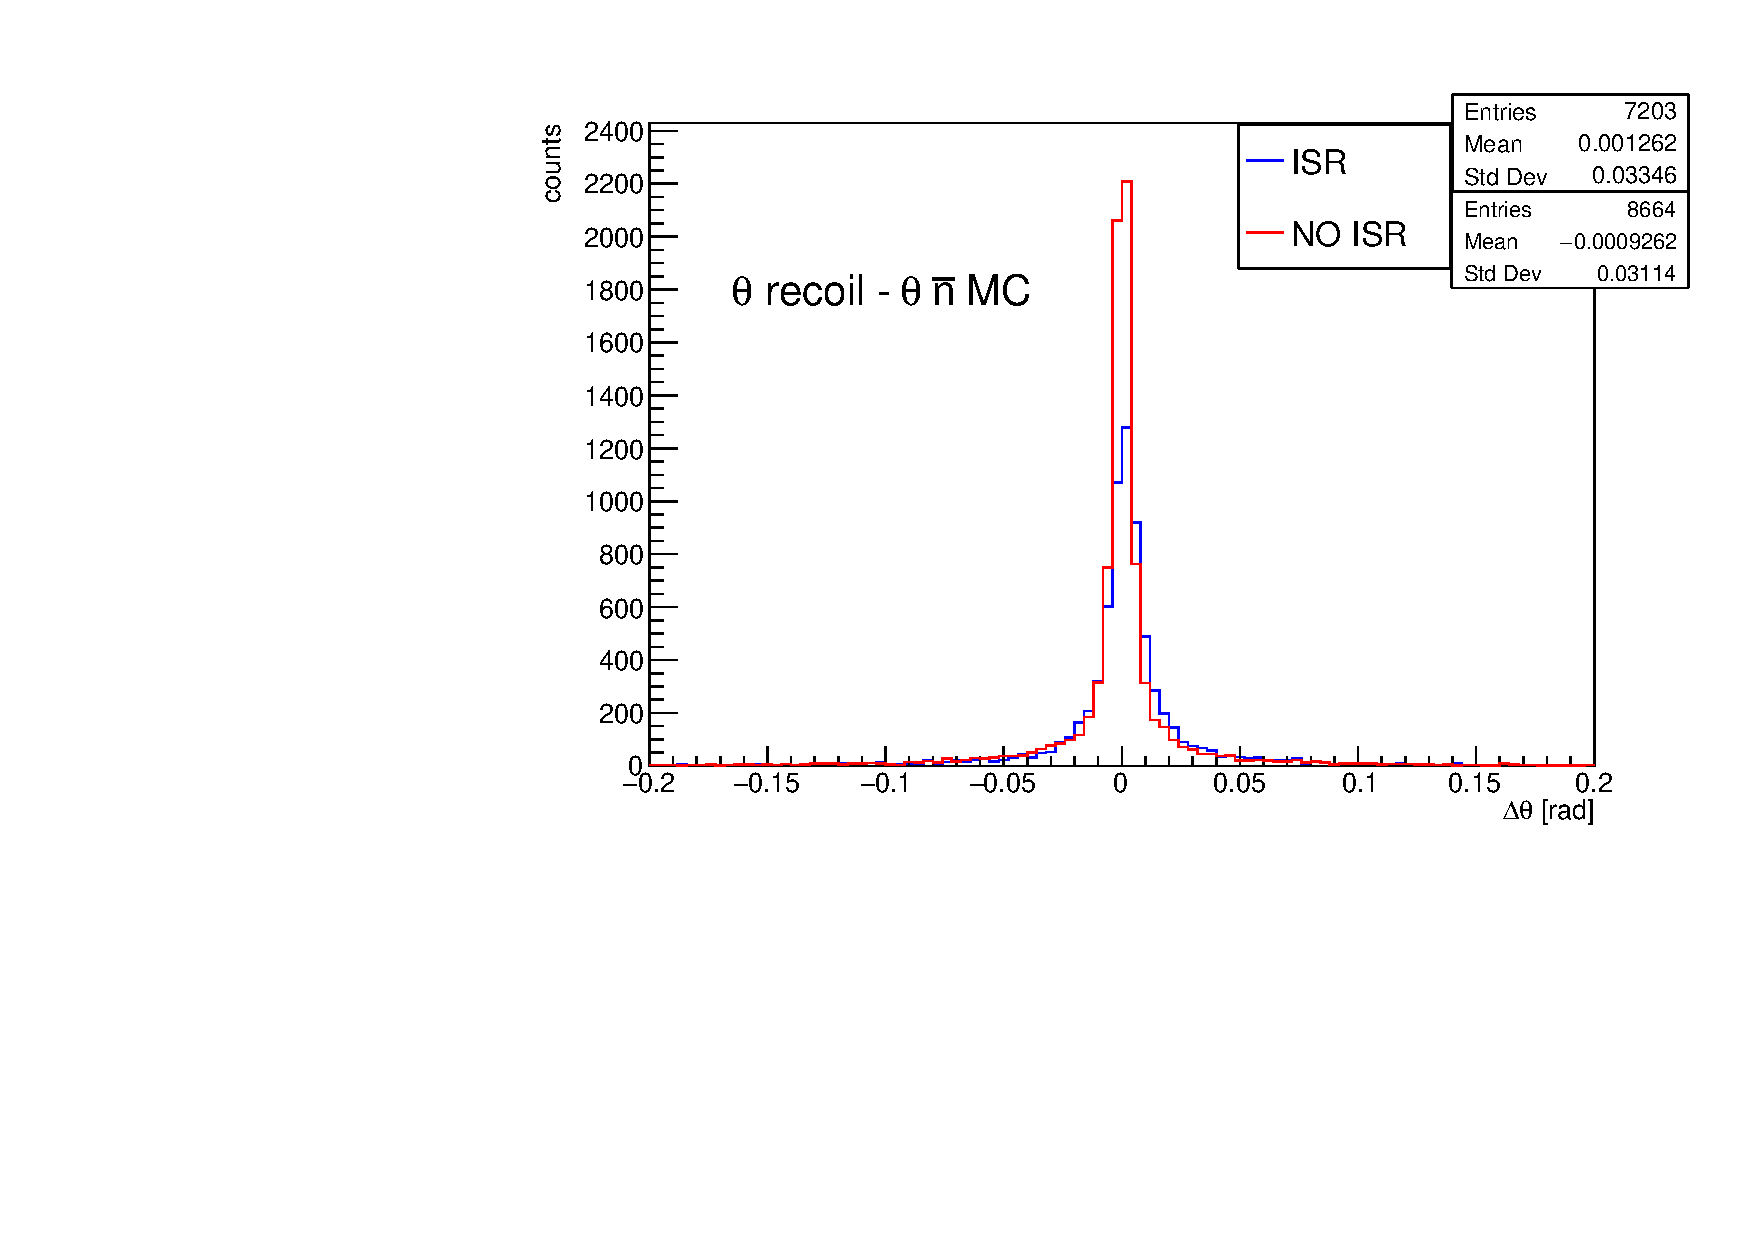
\includegraphics[width=0.49\textwidth]{nbar_MC/images/diff_thetaREC_ntheta_mc.pdf}
     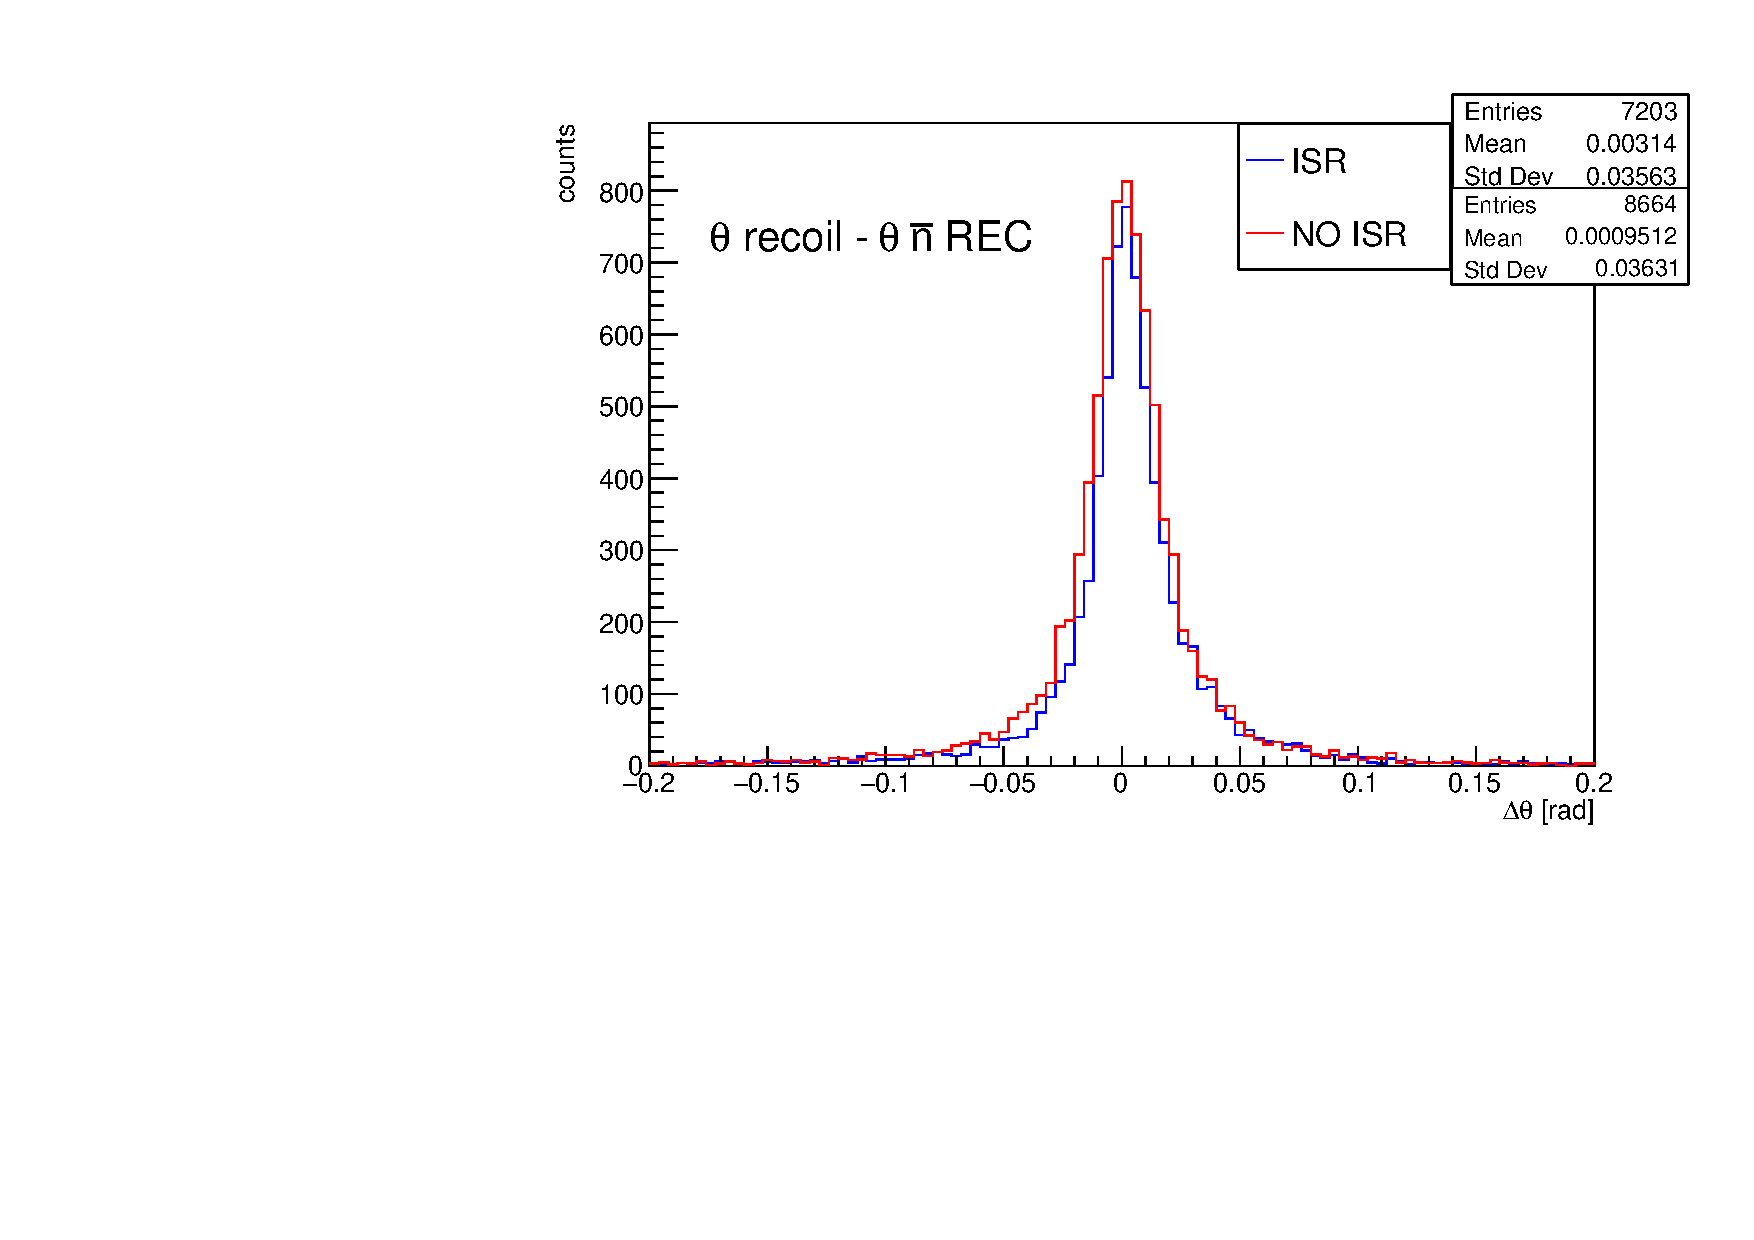
\includegraphics[width=0.49\textwidth]{nbar_MC/images/diff_thetaREC_ntheta_rec.pdf}
     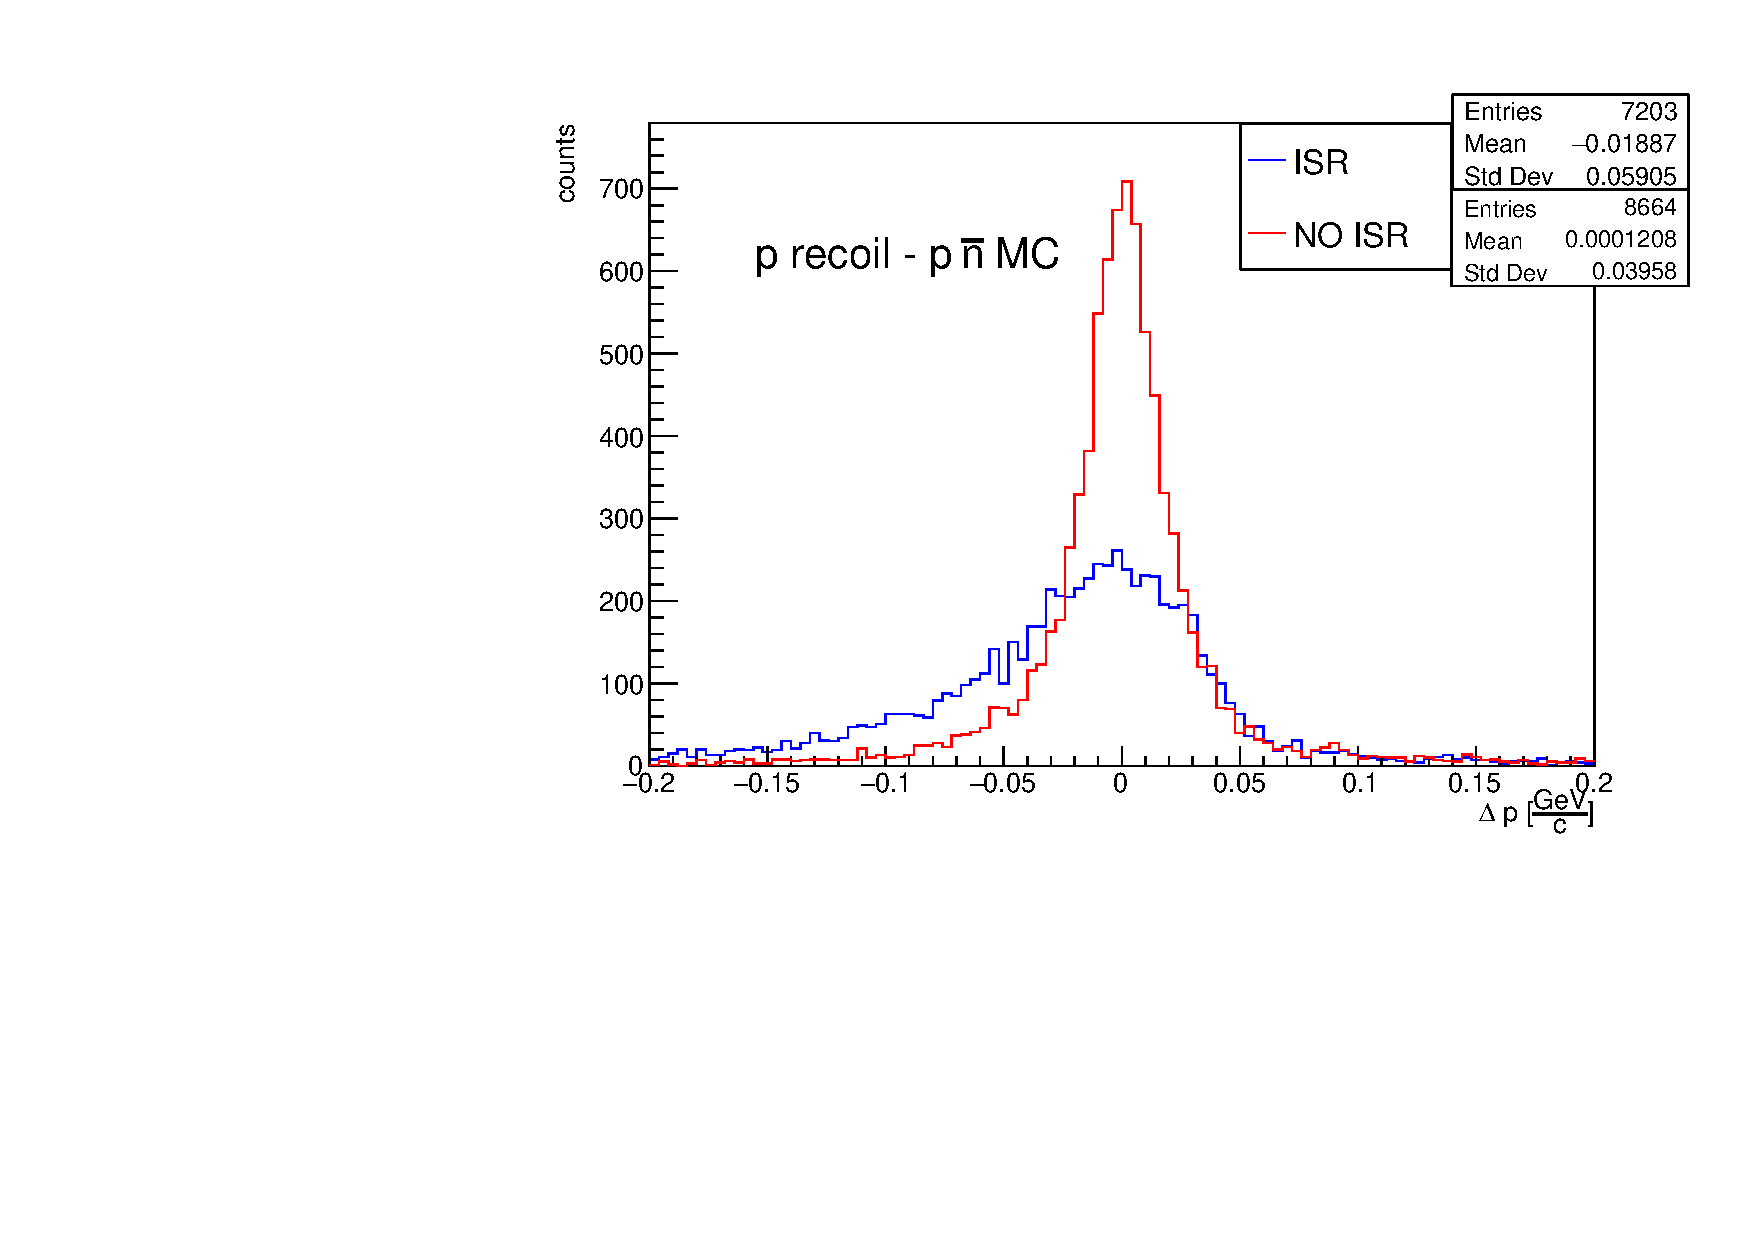
\includegraphics[width=0.49\textwidth]{nbar_MC/images/diff_pREC_np_mc.pdf}
     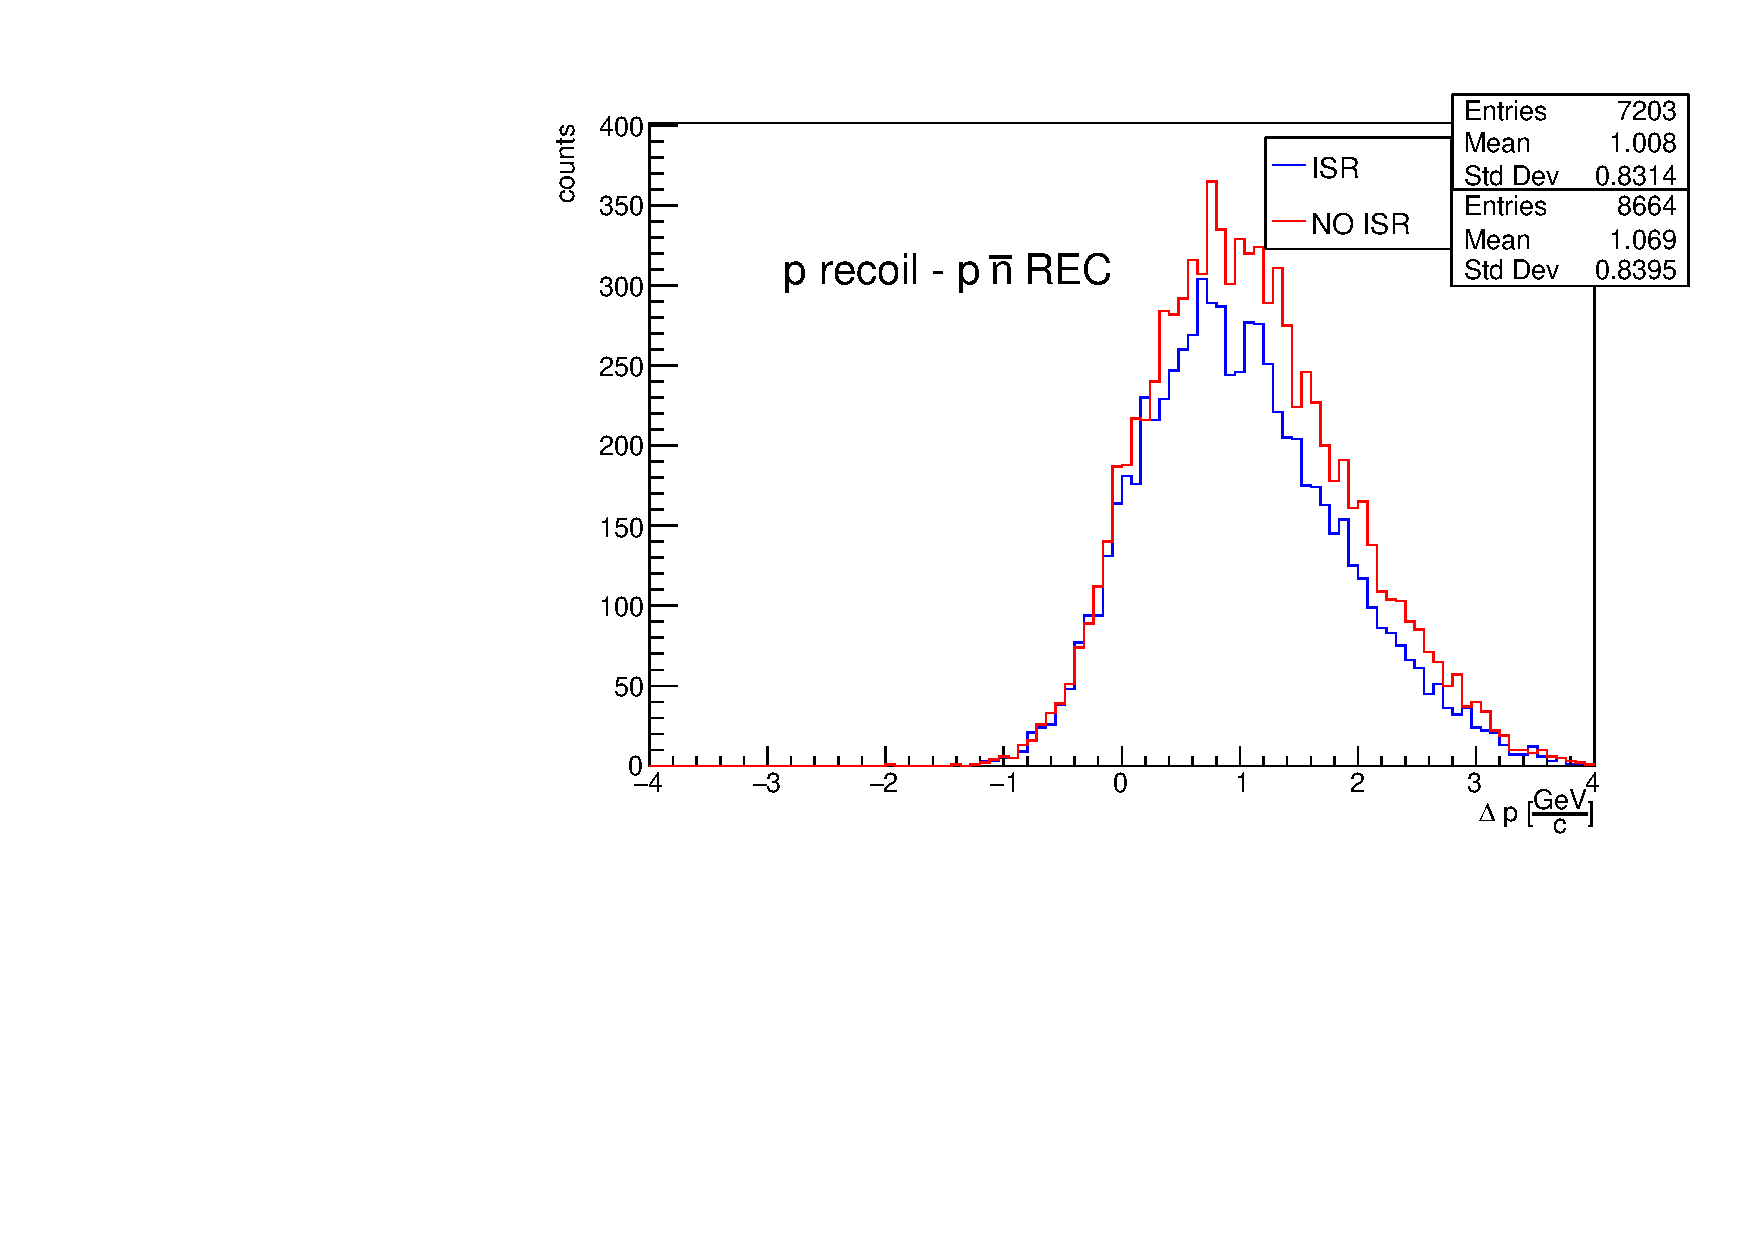
\includegraphics[width=0.49\textwidth]{nbar_MC/images/diff_pREC_np_rec.pdf}
     \caption{Momentum and $\theta$ angle residuals distribution between recoil system and anti-neutron candidate}
\end{figure}

Besides exhibiting poor resolution, the reconstructed momentum of the $\bar{n}$ is underestimated as the residuals distributions show, suggesting a missing energy in the shower. Therefore, the $\bar{n}$ momentum is poorly reconstructed using only the ECL information. Most of anti-neutrons undergo in annihilation with hadrons such as $\bar{n} n$ and $\bar{n} p$, producing pions which escape the calorimeter. Therefore, the reconstructed momentum (or energy) in the calorimeter is not directly comparable with the one of anti-neutrons.
$\\$
\subsection{The $\bar{n}$ ancestors analysis}
As observed, cluster split-off and/or pre-showering effects can occur distorting the $\bar{n}$ reconstructed distributions. 
$\\$
Since the ISR and NO ISR results are analogous, only the ISR case are analyzed on the following section for smoother reading.

 \begin{figure}[H]
    \centering
     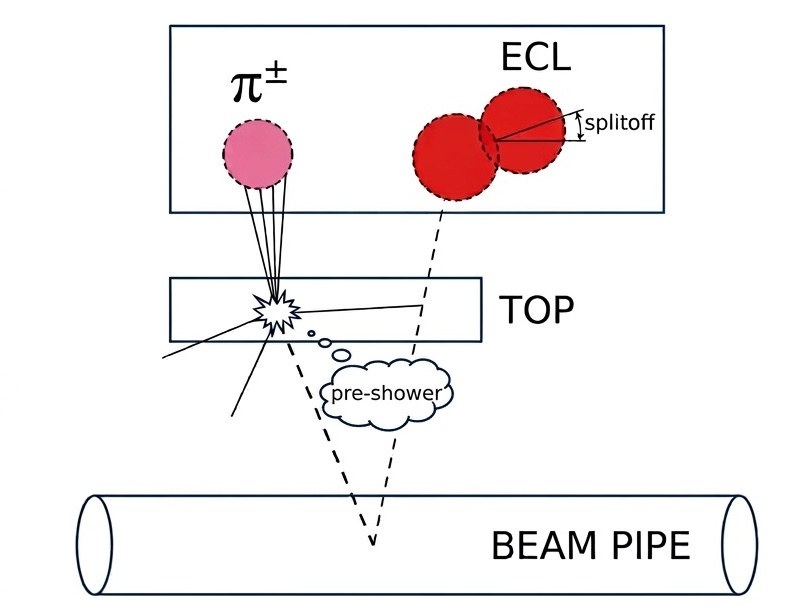
\includegraphics[width=0.55\textwidth]{nbar_MC/images/spoff_pshow}
     \caption{Artistic sketch displaying cluster split-off and pre-showering effects following $\bar{n}$ annihilation. Cluster split-off occurs in the ECL, while pre-showering takes place in the TOP; the respective products then travel toward the ECL and then mis-identified as the primary cluster associated to the anti-neutron}
\end{figure}

The secondary particle from $\bar{n}$ annihilation can be detected as the primary ECL cluster, resulting in information loss and requiring the TOP time information to improve the anti-neutron detection. 
\subsubsection{The ancestor meta-variables}
In order to study the chain and the kinship degree of the neutral cluster associated to $\bar{n}$ candidates detected in the ECL, the basf2 \textbf{ancestor} meta-variables are analyzed, such as:

\begin{itemize}
\item \textbf{varForFirstMCAncestorOfType(type, variable)}: this metavariable returns the requested \textbf{variable} of the first ancestor of the given \textbf{type}  -a specific particle- found in a certain point of the chain

\item \textbf{hasAncestor(PDG, abs)}: this metavariable returns a positive integer if an ancestor -a certain relatives in the cahin- with the given \textbf{PDG} code is found, 0 otherwise. It means thats 1 = first mother, 2 = grandmother, etc. Second argument \textbf{abs} is optional: 1 means that the sign of the PDG code is taken into account, default is 0
\end{itemize}

A typical scenarios of $\bar{n}$ as ancestor could  be the following:
\begin{center}
0)$\bar{n}$ from IP $\rightarrow$ 1)$\bar{n}$ annihilation in TOP (pions produced) $\rightarrow$ 2) pions detected 
0)$\bar{n}$ from IP $\rightarrow$ 1)$\bar{n}$ annihilation in ECL (pions produced) $\rightarrow$ 2) pions detected
\end{center}

Therefore the variables \textbf{varForFirstMCAncestorOfType(anti-n0, p)} and \textbf{hasAncestor(-2112, 1)} of neutral cluster associated to $\bar{n}$ are discussed. Given the close similarity between the results, only the ISR case is discussed. The hasAncestor distribution is shown below:
 \begin{figure}[H]
    \centering
     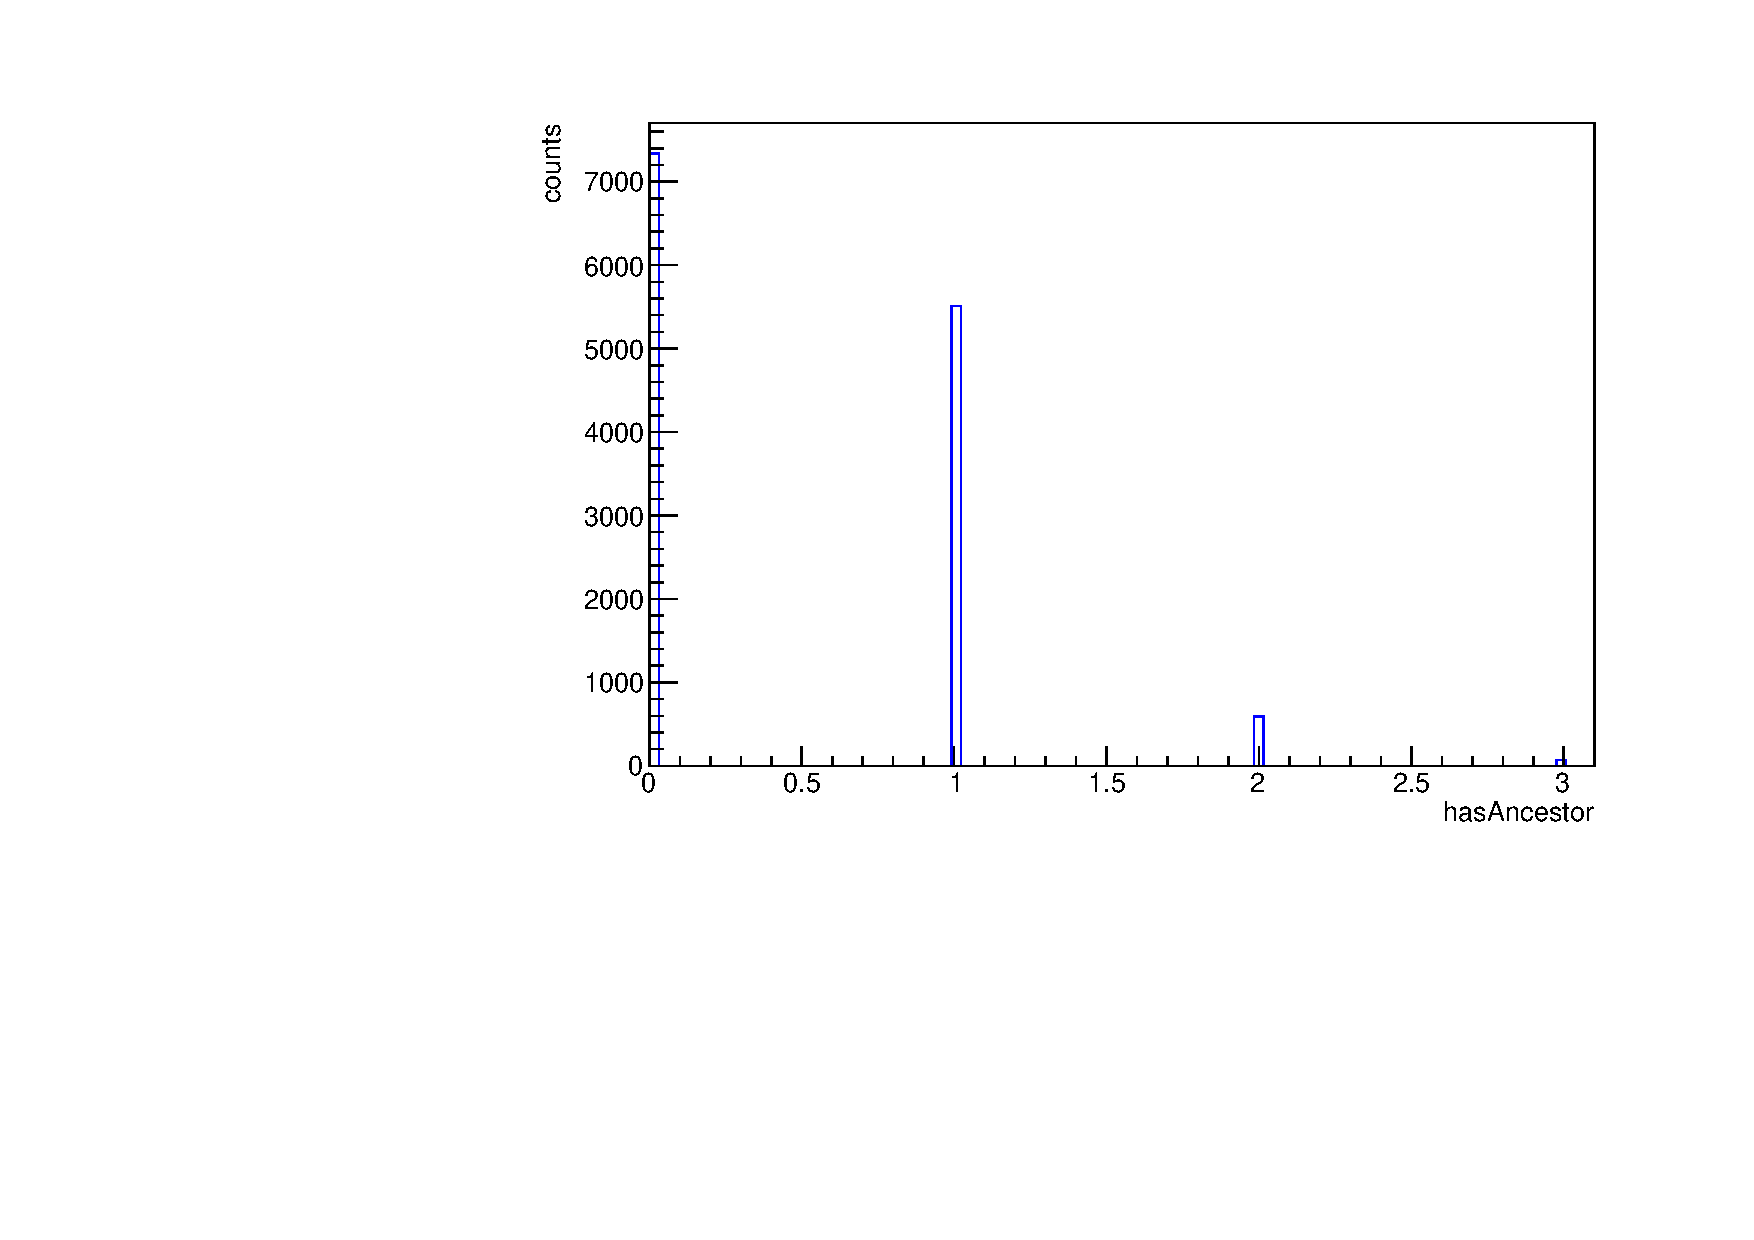
\includegraphics[width=0.70\textwidth]{nbar_MC/images/hasAncestor.pdf}
     \caption{Distribution of the ancestry kinship degree of anti-neutron candidates with an anti-neutron present in their ancestry chain}
\end{figure}

Consequently, most $\bar{n}$ candidates lack an $\bar{n}$ in their relative chain (has\_Ancestor=0), suggesting they are the primary $\bar{n}$ themselves. The second contribution is made of $\bar{n}$ candidates having $\bar{n}$ as mother etc. 
$\\$
In order to directly study the contribution of each term, it could be useful to access to the Monte Carlo truth and look at the PID trough the \textbf{mc\_PDG}, which basically is the real PDG of the selected candidates coming from the generator. The obtained distributions are shown below:

 \begin{figure}[H]
    \centering
    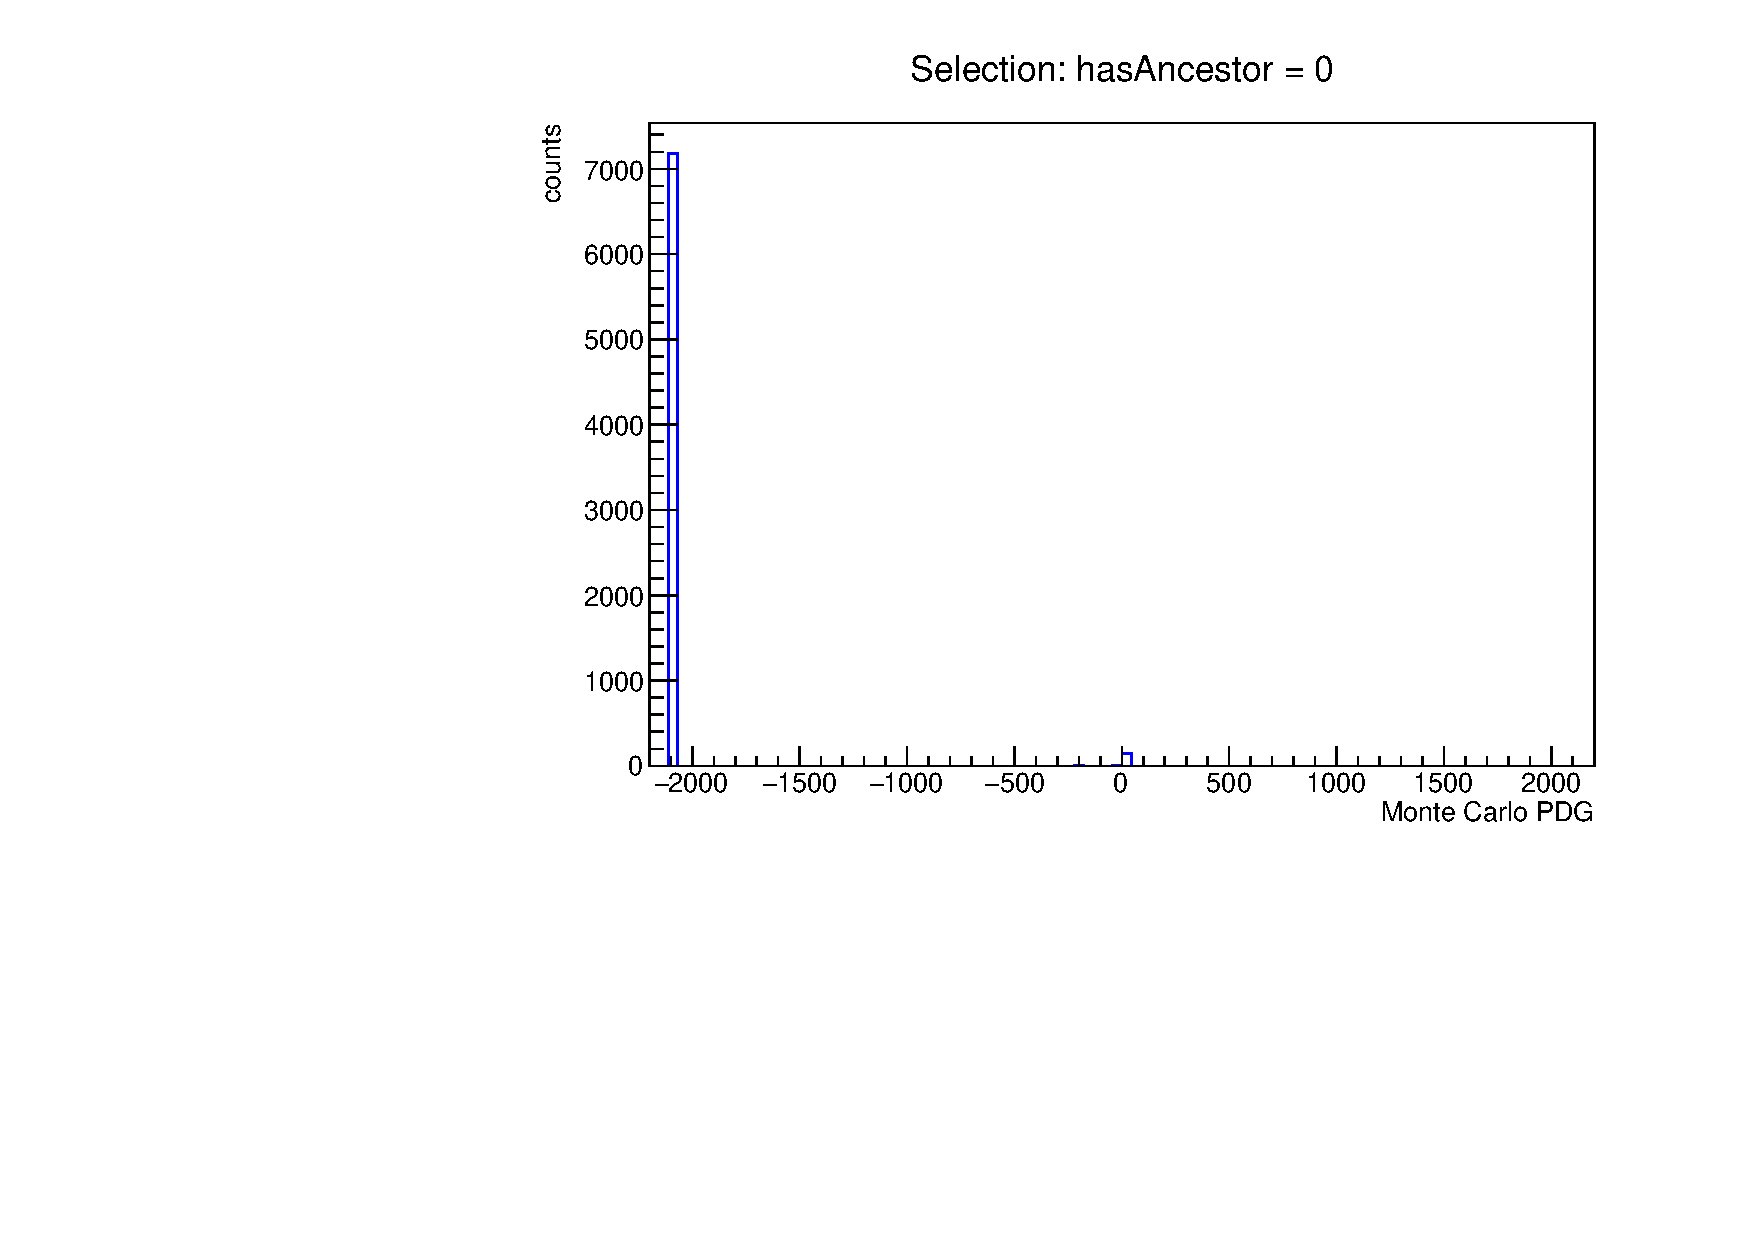
\includegraphics[width=0.49\textwidth]{nbar_MC/images/mc_pdg_hasAncestor=0.pdf}
    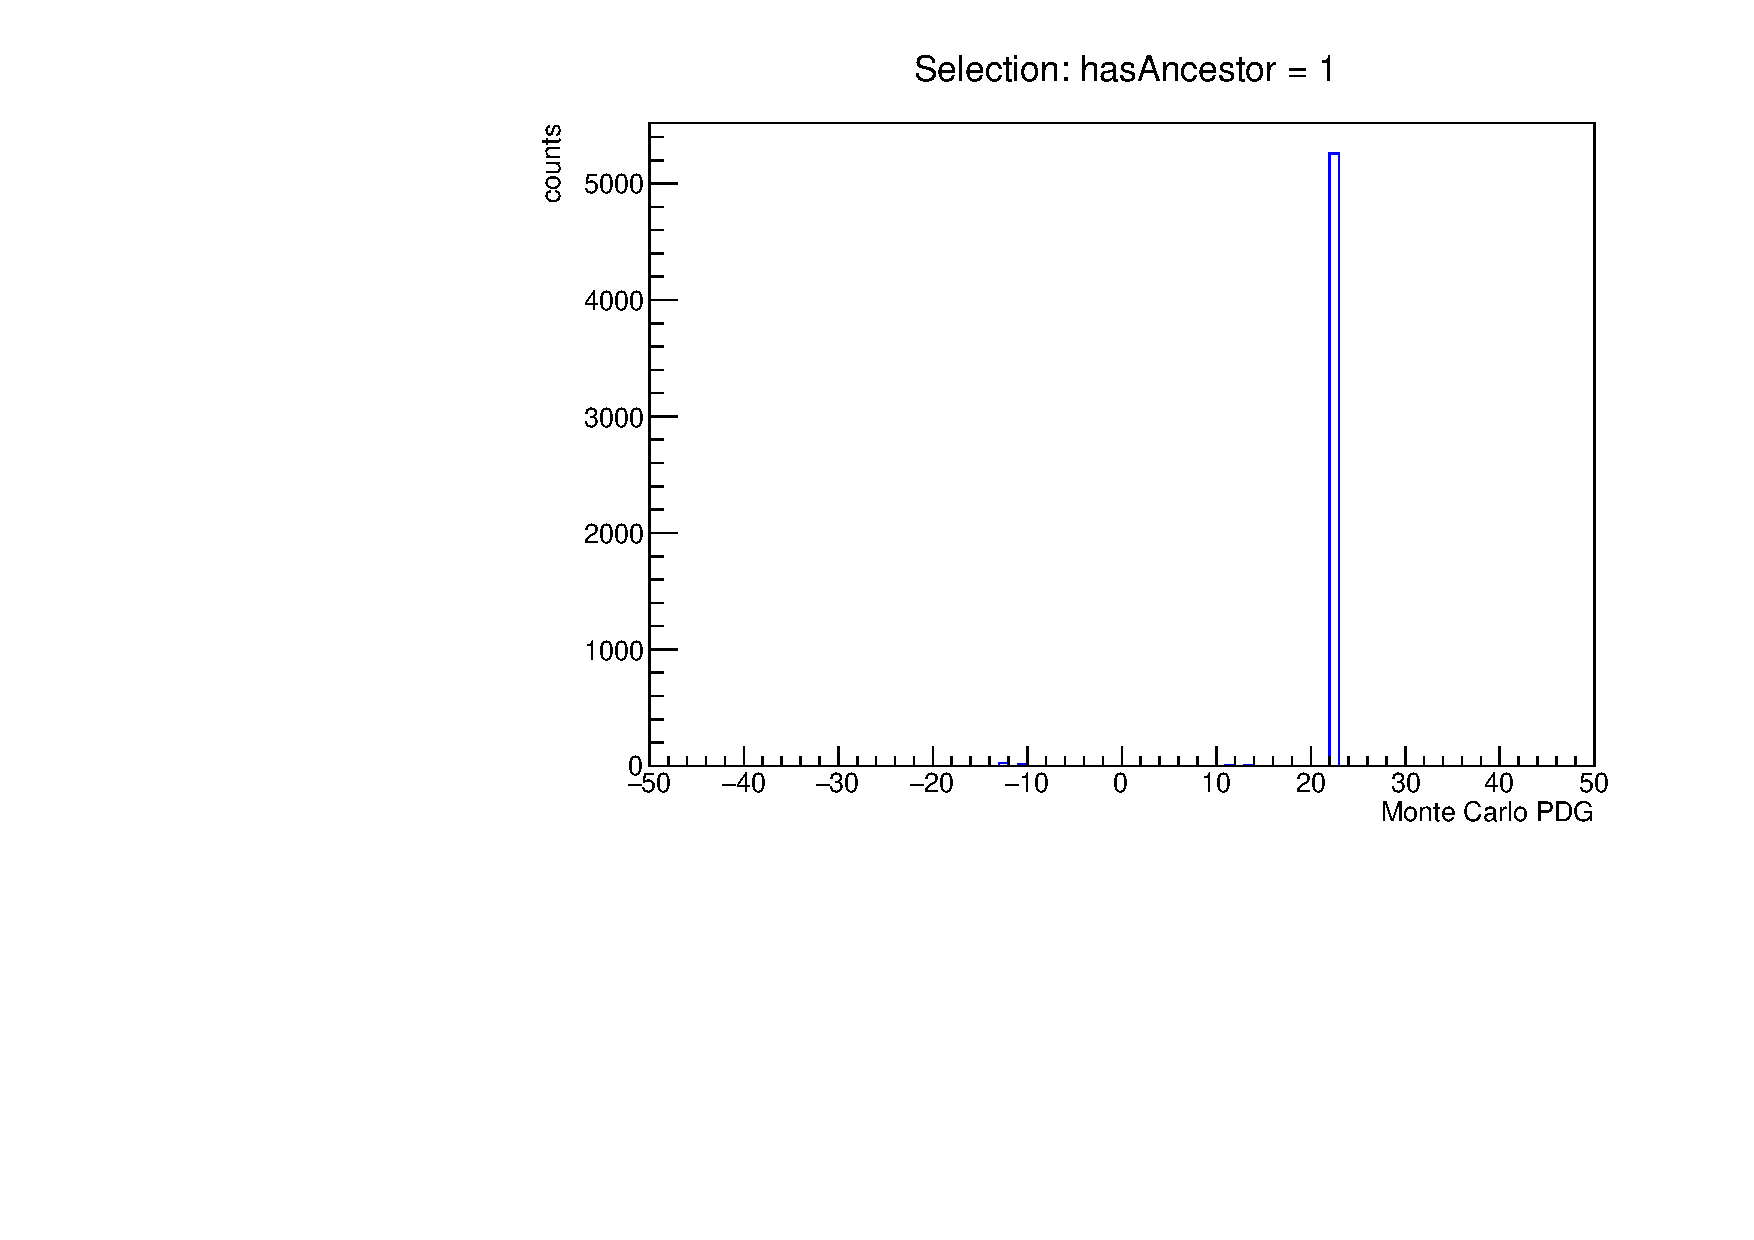
\includegraphics[width=0.49\textwidth]{nbar_MC/images/mc_pdg_hasAncestor=1.pdf}
     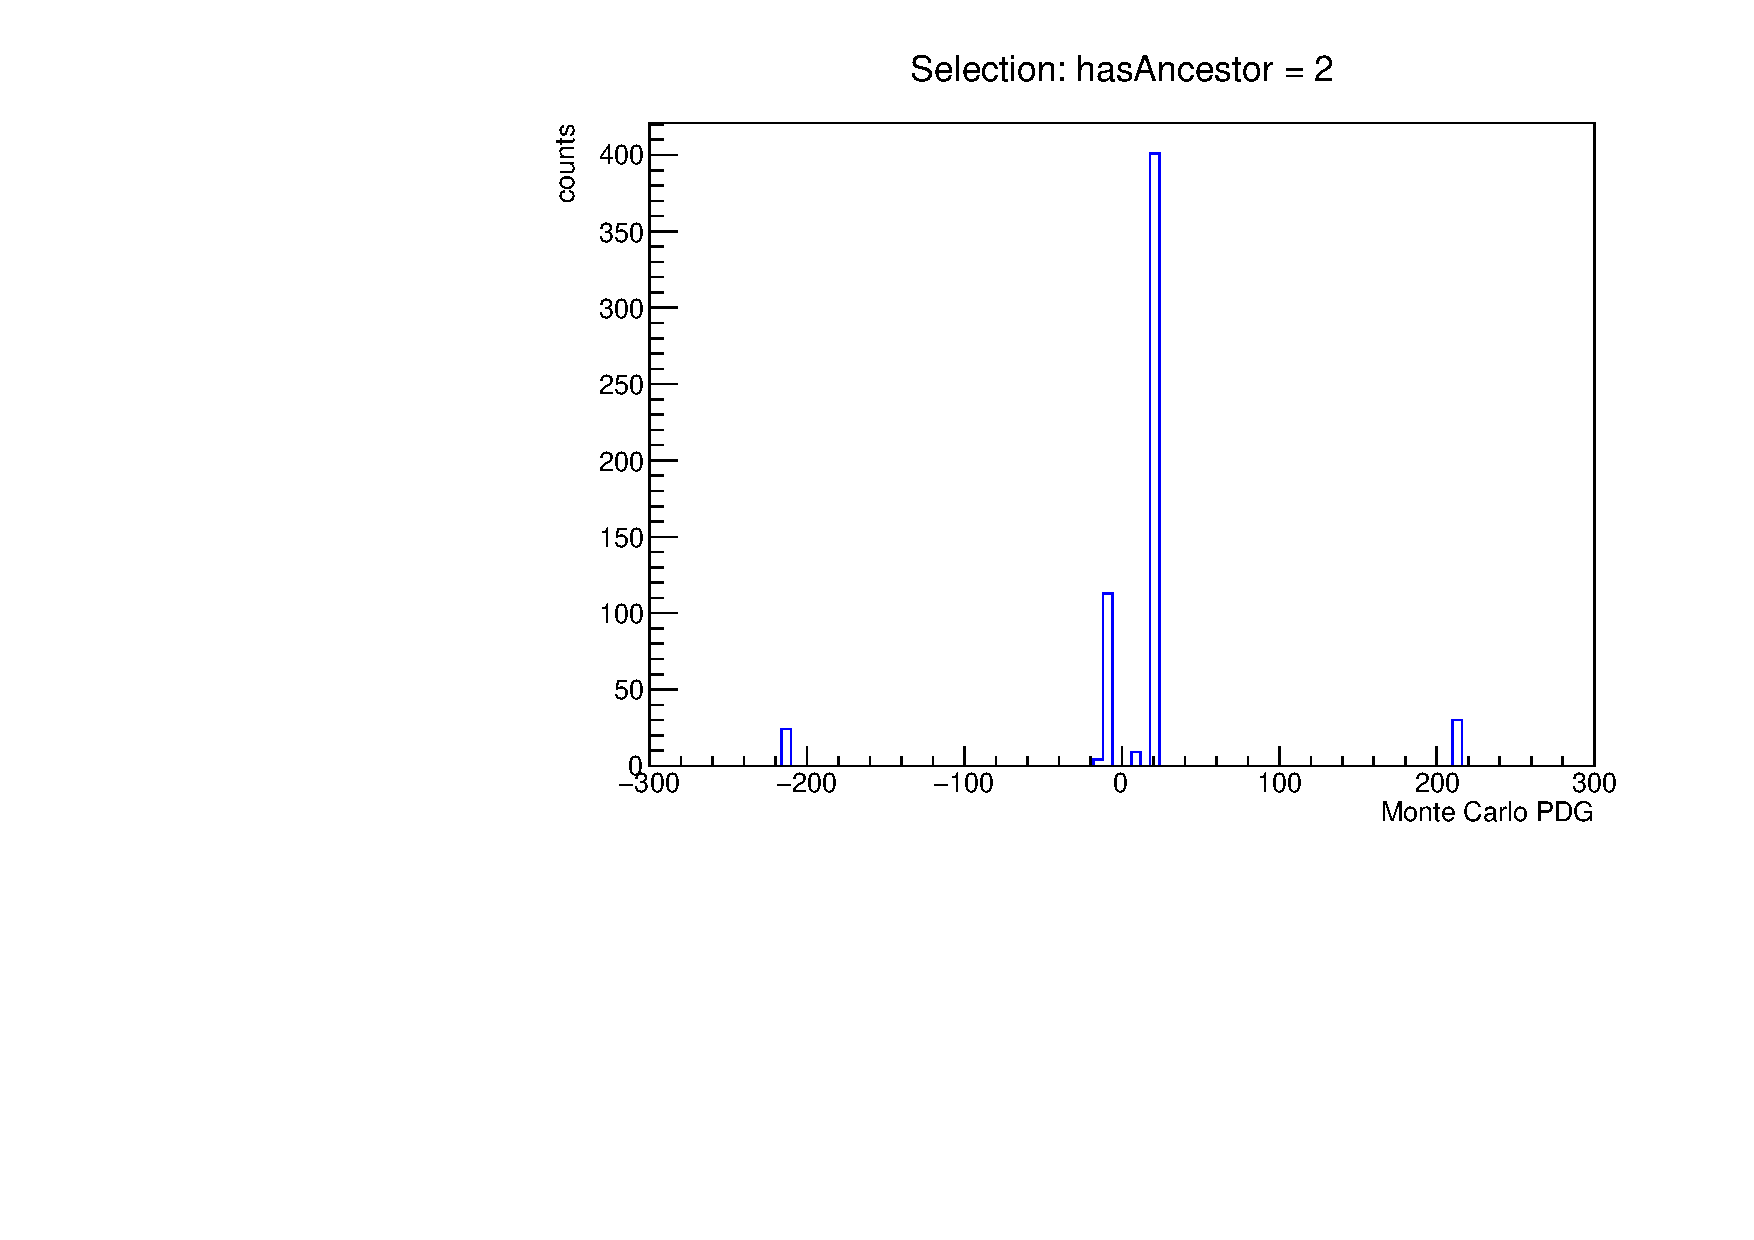
\includegraphics[width=0.49\textwidth]{nbar_MC/images/mc_pdg_hasAncestor=2.pdf}
     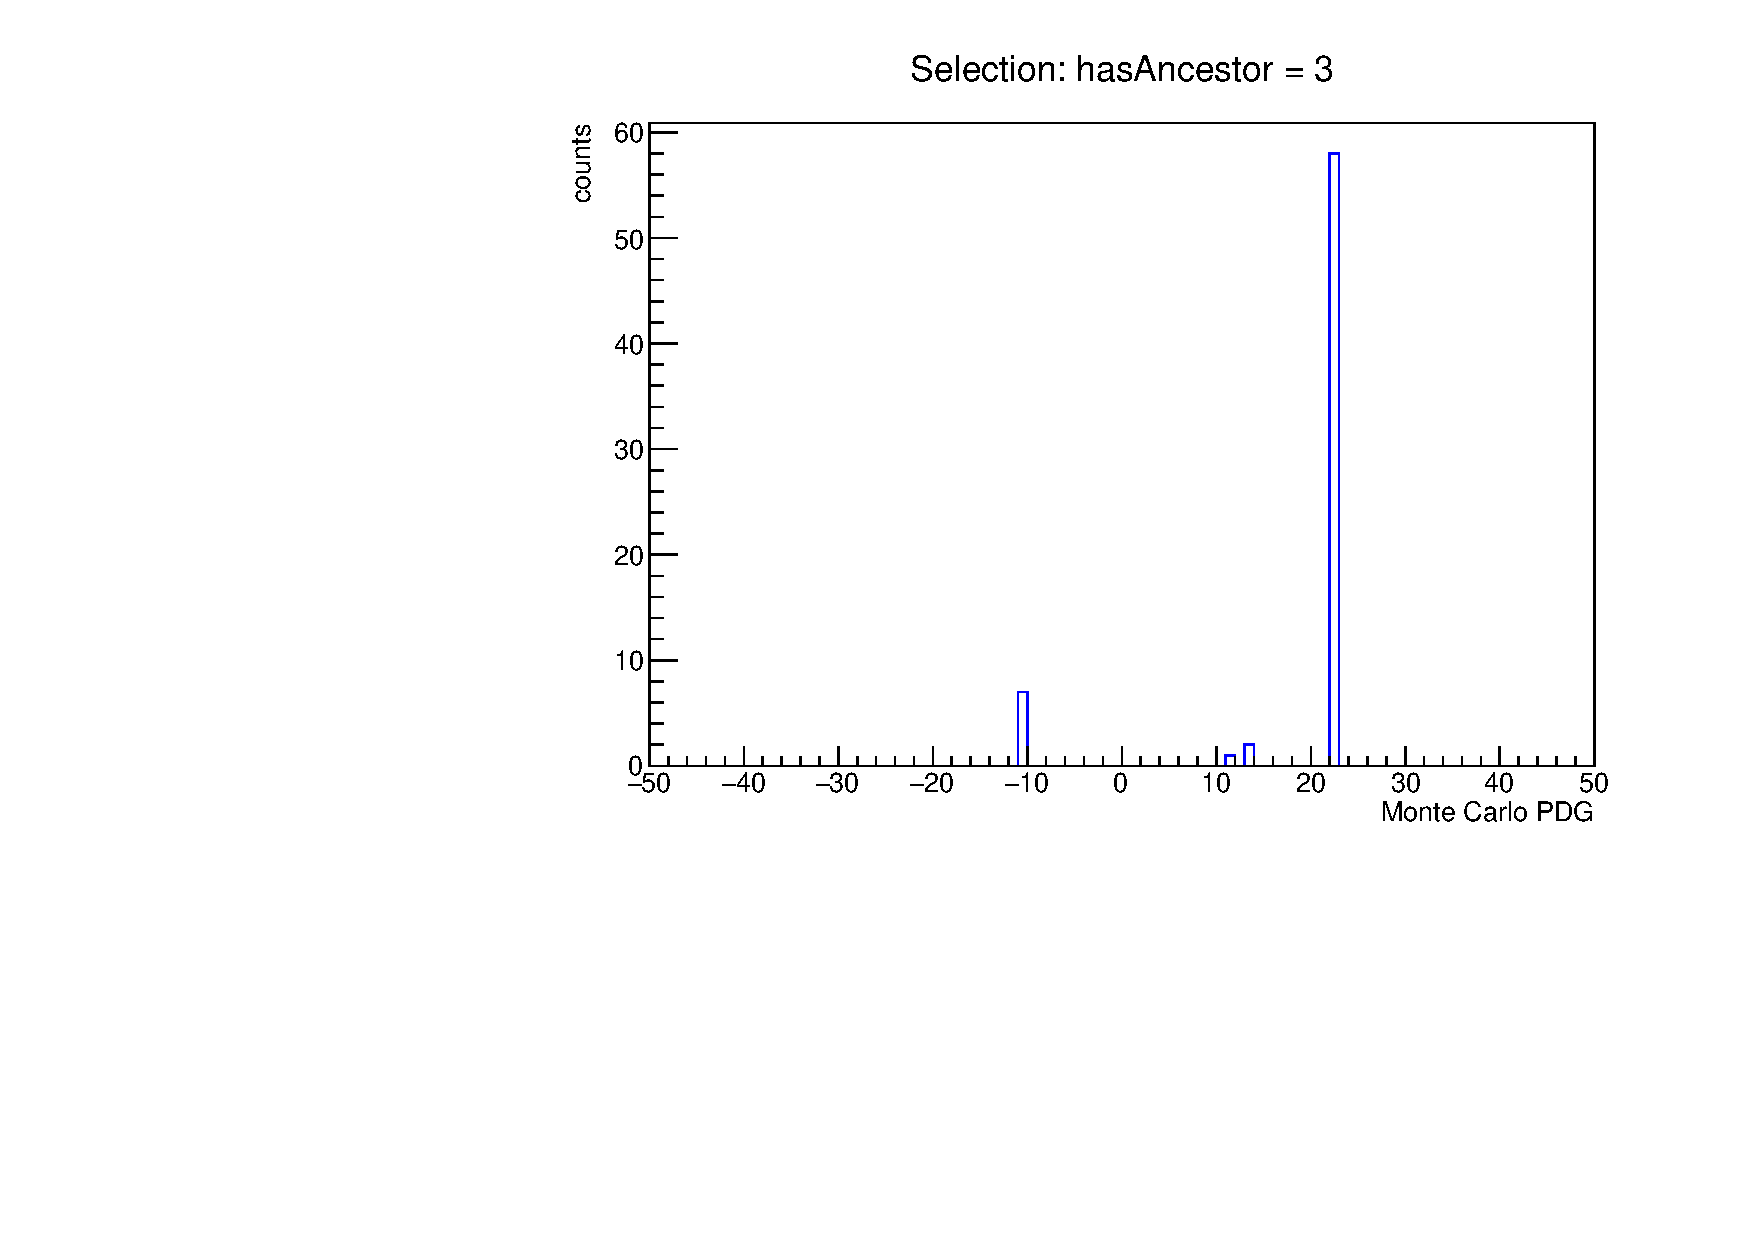
\includegraphics[width=0.49\textwidth]{nbar_MC/images/mc_pdg_hasAncestor=3.pdf}
     \caption{Monte Carlo PDG codes of candidates with degrees of ancestry selection. As mentioned, the MC PDG variable reveals the generator-level identity of the reconstructed particle by providing its PDG code}
\end{figure}

\begin{itemize}
\item \textbf{hasAncestor = 0} clearly shows that $\bar{n}$ candidates without an $\bar{n}$ as relatives are mainly true anti-neutrons, as their Monte Carlo PDG code is primarily -2112.This is consistent since the anti-neutron comes from the IP and it is directly detected in the ECL through its own annihilation
\item \textbf{hasAncestor = 1}  shows that the $\bar{n}$ candidates with an $\bar{n}$ as mother are predominately gammas (Monte Carlo PDG = 22), suggesting they result from $\bar{n}$ interactions prior to $\bar{n}$ candidate  ECL cluster formation
\item \textbf{hasAncestor = 2} suggests that the $\bar{n}$ candidates with an $\bar{n}$ as grandmother are mainly gammas, with some spurious pions (-211 \& +211) and electrons or positrons (+11 \& -11). The case with hasAncestor = 3 yields analogous results
\end{itemize}

\subsubsection{Ancestor momentum}
The figure ~\ref{fig:pRecoil_nmcP} can be updated, by including the momentum of the ancestors obtained with \textbf{varForFirstMCAncestorOfType(anti-n0, p)}. The idea is to check if the information from the first structure -the one at low value of momentum- can be recovered using the ancestors chain. The obtained distributions are shown below:

 \begin{figure}[H]
    \centering
    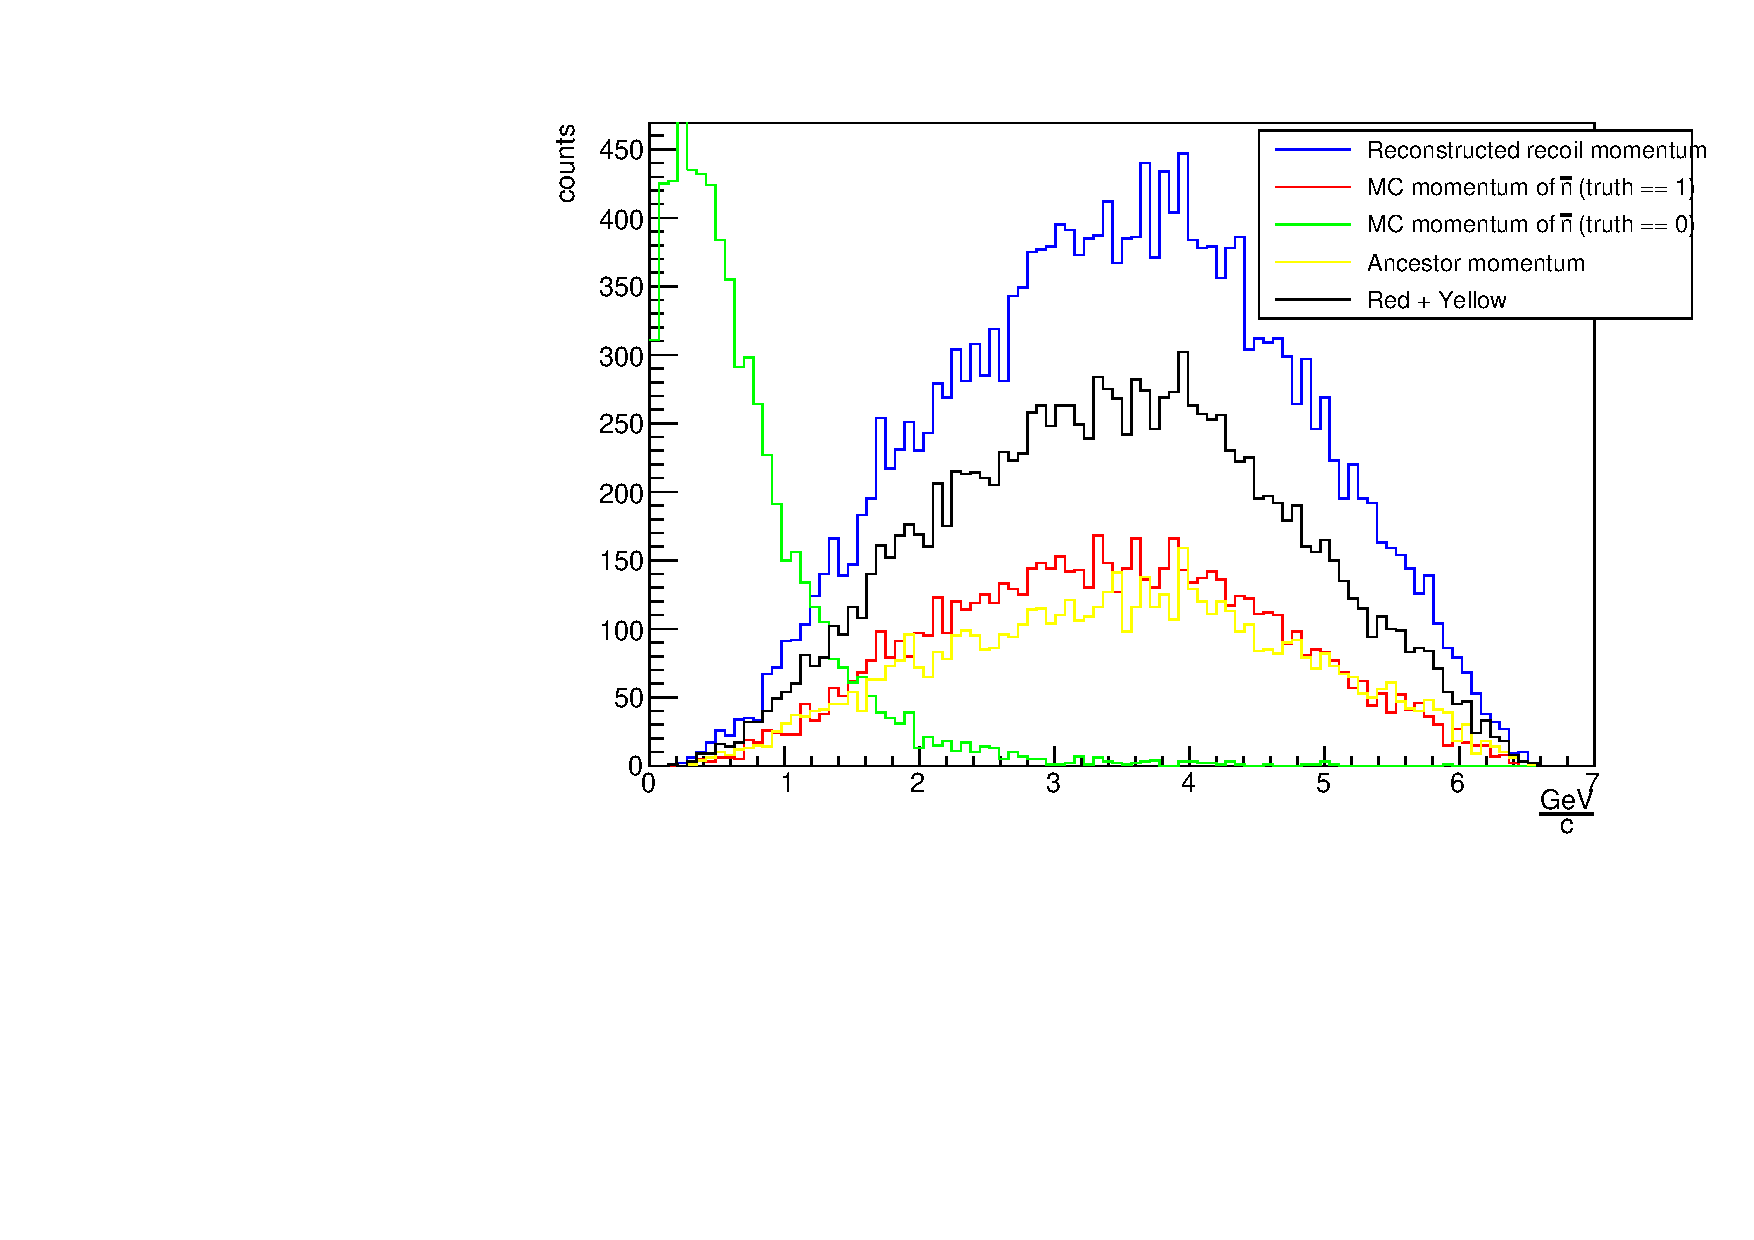
\includegraphics[width=0.7\textwidth]{nbar_MC/images/momentum_ancestors.pdf}
    \caption{Momentum comparison of different components. The recoil vector is the only reconstructed variable, while the others are obtained from Monte Carlo truth selection, as shown in the legend}
\end{figure}

The {\color{blue} blue distribution} is made of 20146 entries, the {\color{red} red one} is made of 7203 entries, the {\color{green} green one} is made of 6308 entries, the {\color{yellow} yellow one} is made of 6173 entries and the {\color{black} black one} is made of 13376 entries. It means the 98\% of the first structure is recovered by ancestor momentum, suggesting that phenomena prior to neutral cluster associated to $\bar{n}$ candidates can occur, such as cluster split-off and pre-showering.
$\\$
The quality of the ancestor momentum can be discussed by studying the residuals with respect to the reconstructed recoil momentum:
 \begin{figure}[H]
    \centering
    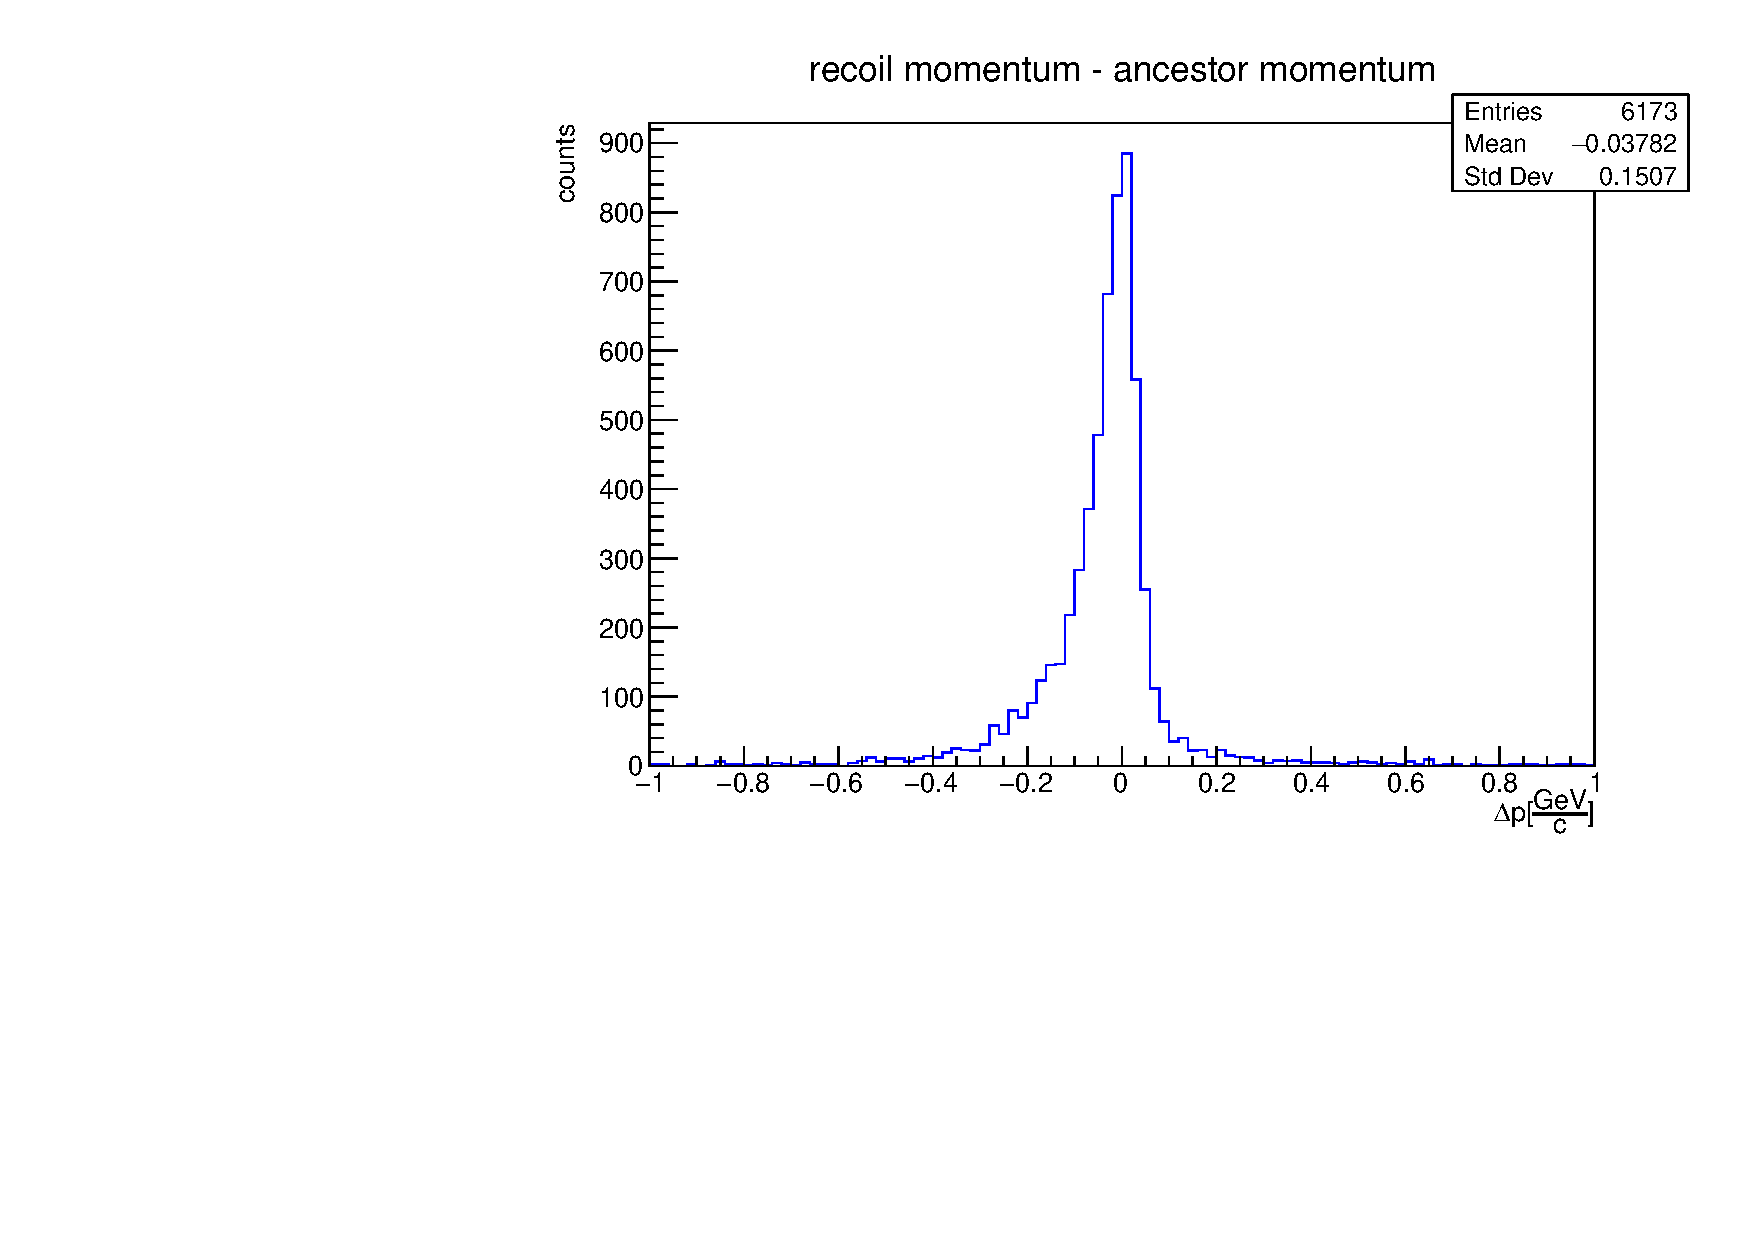
\includegraphics[width=0.7\textwidth]{nbar_MC/images/deltaP_ancestors.pdf}
    \caption{Residual distribution of ancestor momentum with respect to the recoil vector}
\end{figure}

Therefore the reconstructed recoil momentum is a good estimator of the ancestor momentum as well, confirming that cluster split-off or pre-showering may occur prior the ECL cluster formation.
$\\$
It is interesting as well to note that {\color{blue} 20146} - {\color{black} 13376} = 6779 which exactly matches the number of $\bar{n}$ candidates associated with a \textbf{NaN} value, mainly particles that did not receive a correct Monte Carlo association during MC truth matching. They cannot be recovered. The meta-variable \textbf{mcErrors} shows as a bit number the reason why the Monte Carlo fails the association. This variable explicitly shows this behavior:

 \begin{figure}[H]
    \centering
    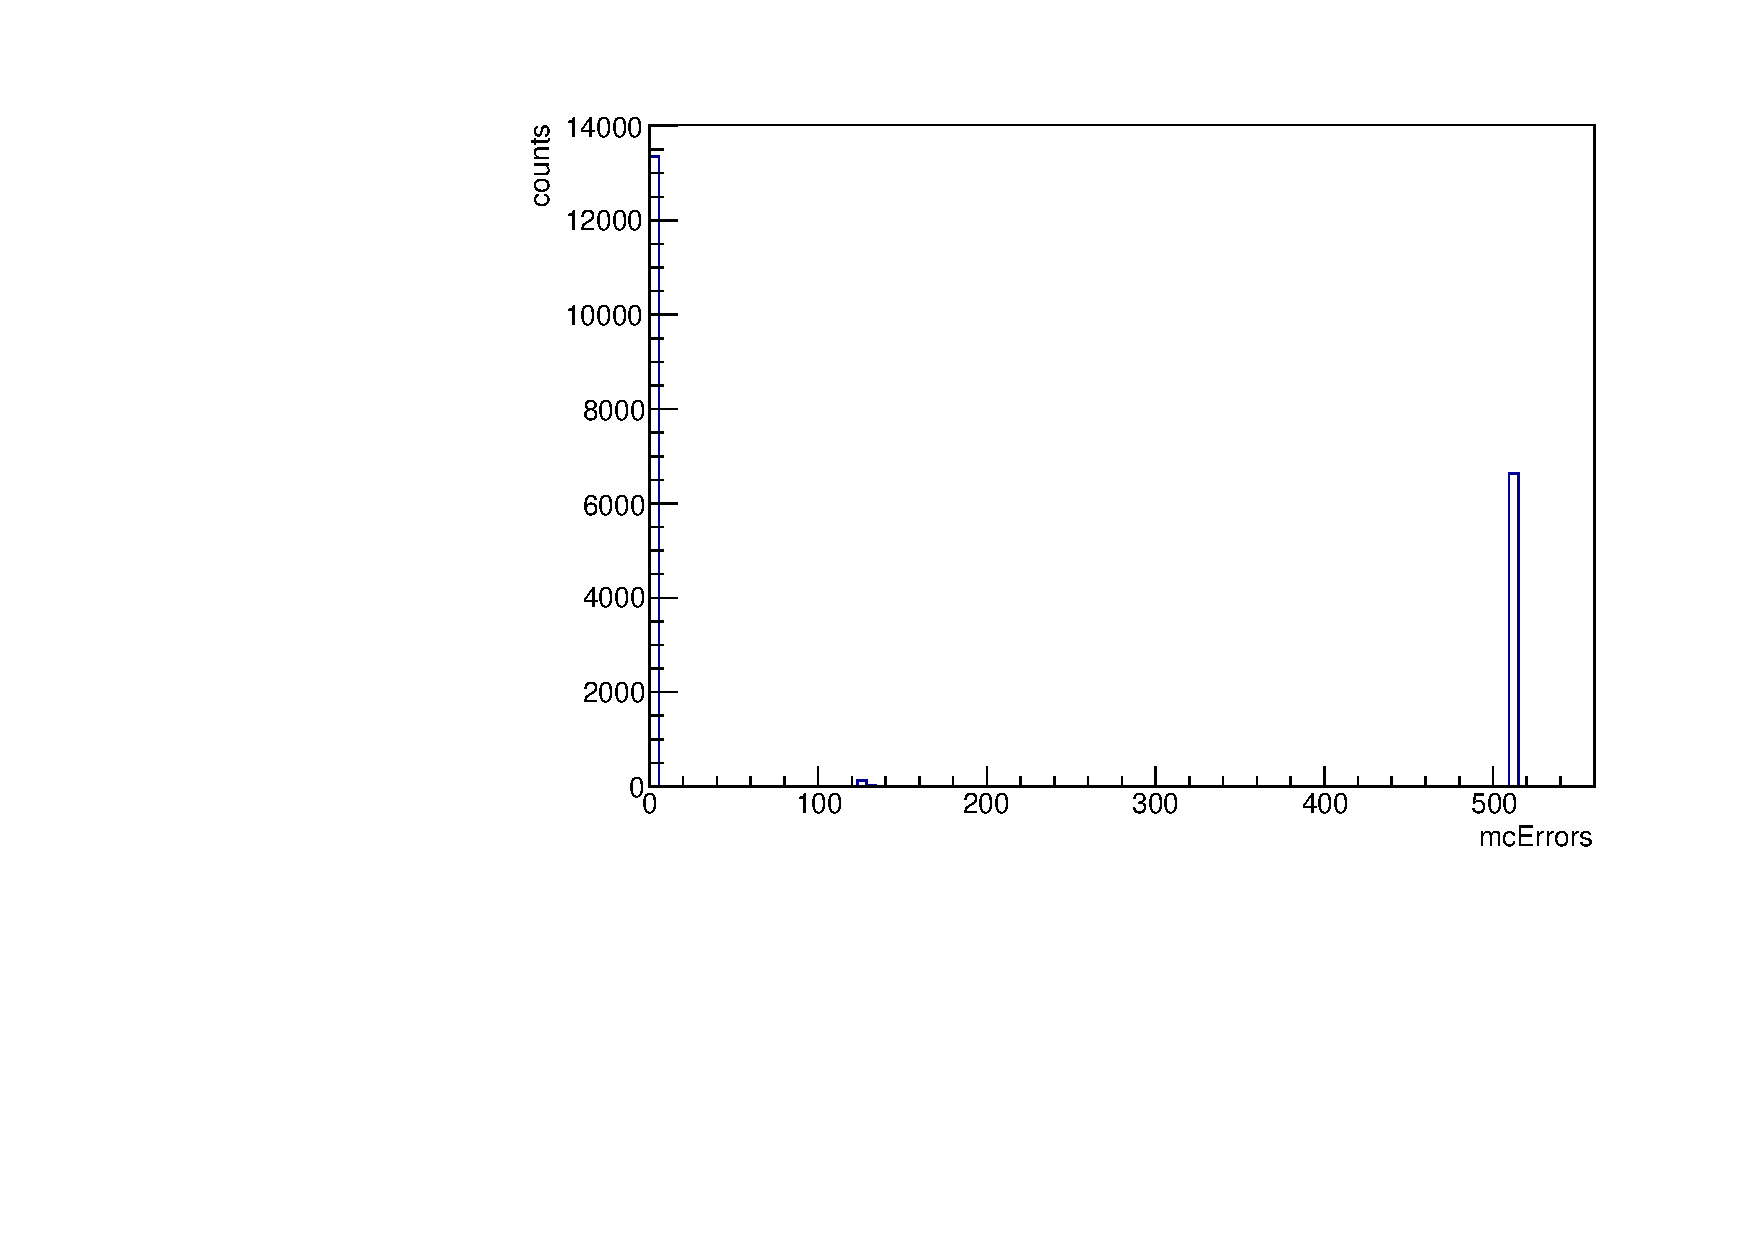
\includegraphics[width=0.7\textwidth]{nbar_MC/images/mcErrors.pdf}
\end{figure}

Where the first peak is above the code \textbf{0}, which means that "\emph{This particle and all its daughters are perfectly reconstructed}", while the second peak is above the code \textbf{512}, which confirms that "\emph{There was an error in MC matching. Not a valid match. Might indicate fake/background track or cluster}", as expected.

\subsubsection{$\bar{n}$ vertex production}
Eventually, in order to a comprehensive ancestor analysis, it could be useful to discuss the generator-level radial production distance $\rho = \sqrt{x^2 + y^2}$ -the vertex production- of $\bar{n}$ candidates, from the z-axis. 
$\\$
To provide a clear overview of $\rho$, the distribution is splitted in two parts: the left part -close to the collision diamond- ($\rho \in [0,0.1]$ cm) and the right part -far from the collision diamond- ($\rho \in (0.1,220]$ cm). The obtained result is shown below:
 \begin{figure}[H]
    \centering
    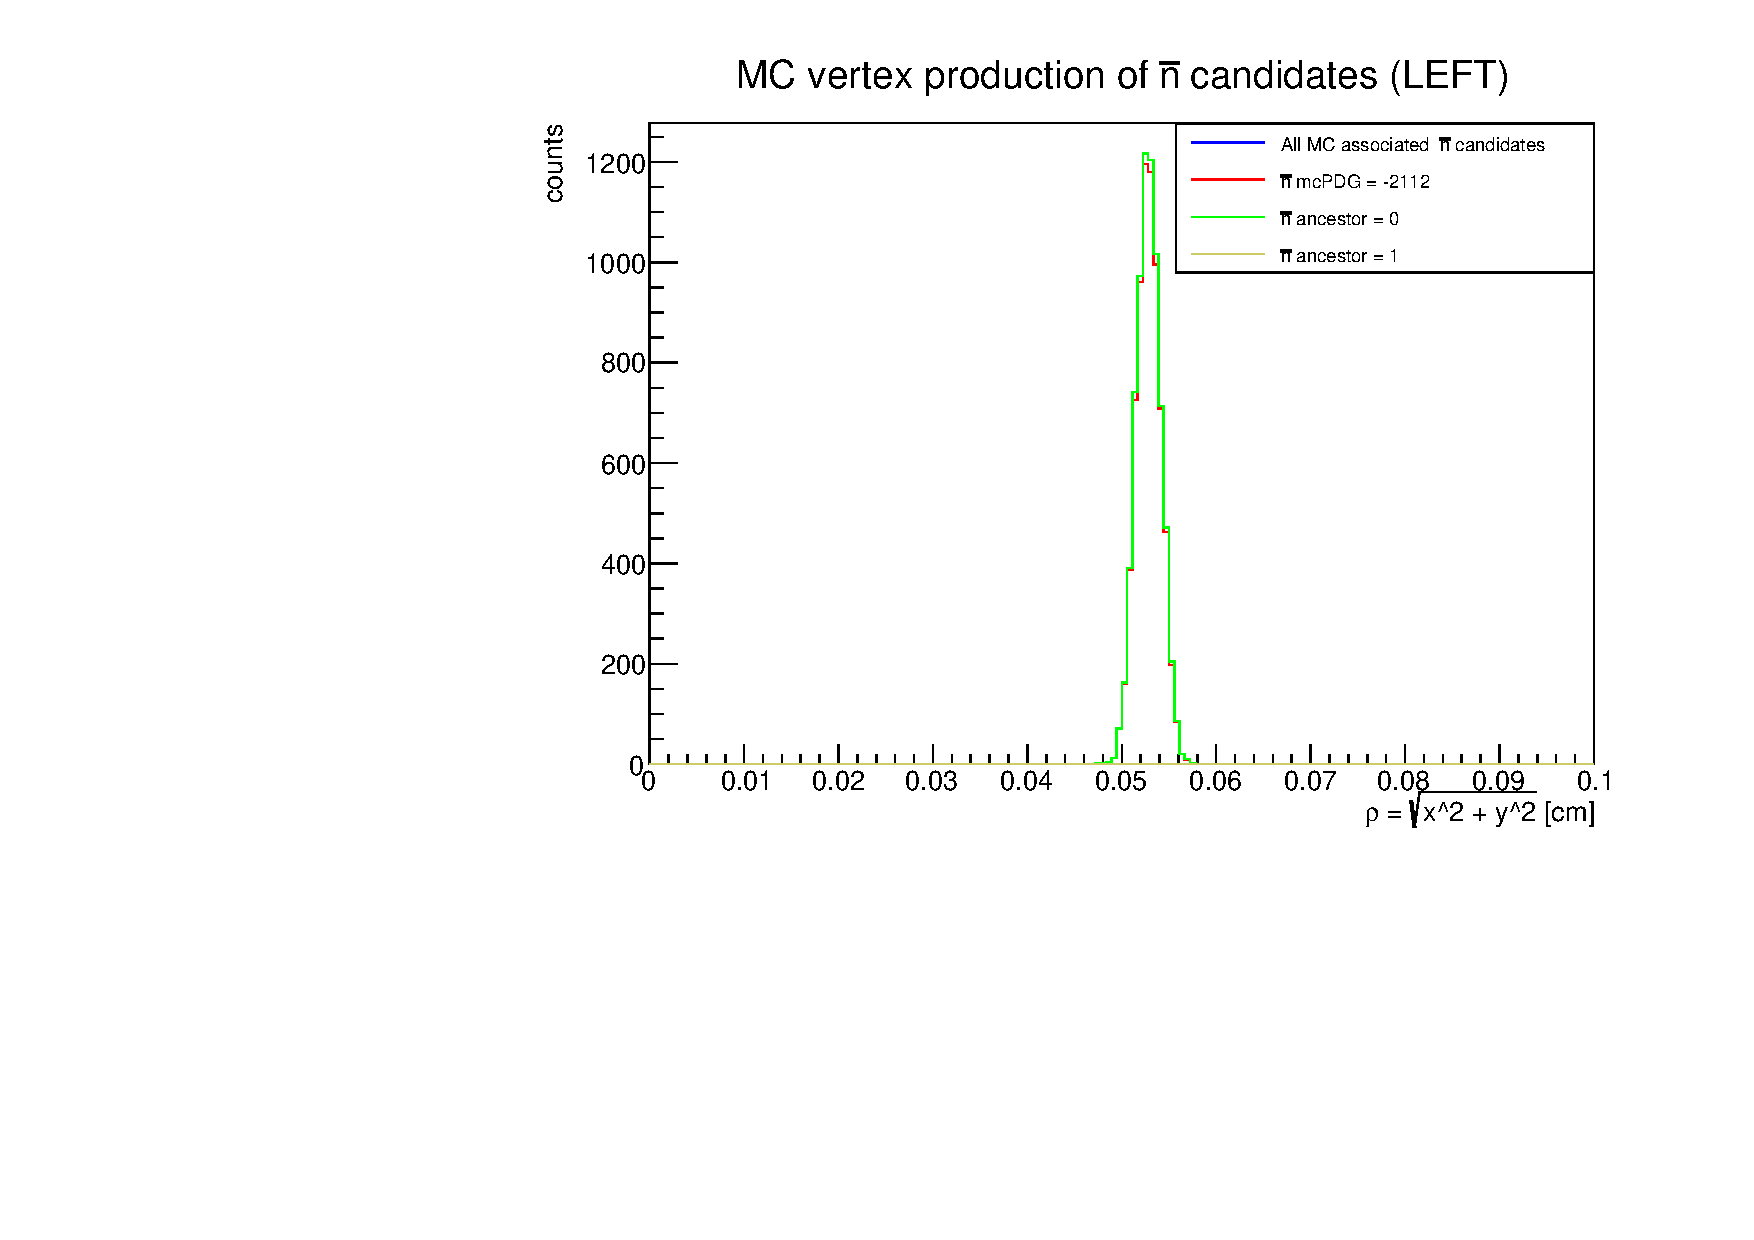
\includegraphics[width=0.49\textwidth]{nbar_MC/images/mcDistance_sx.pdf}
    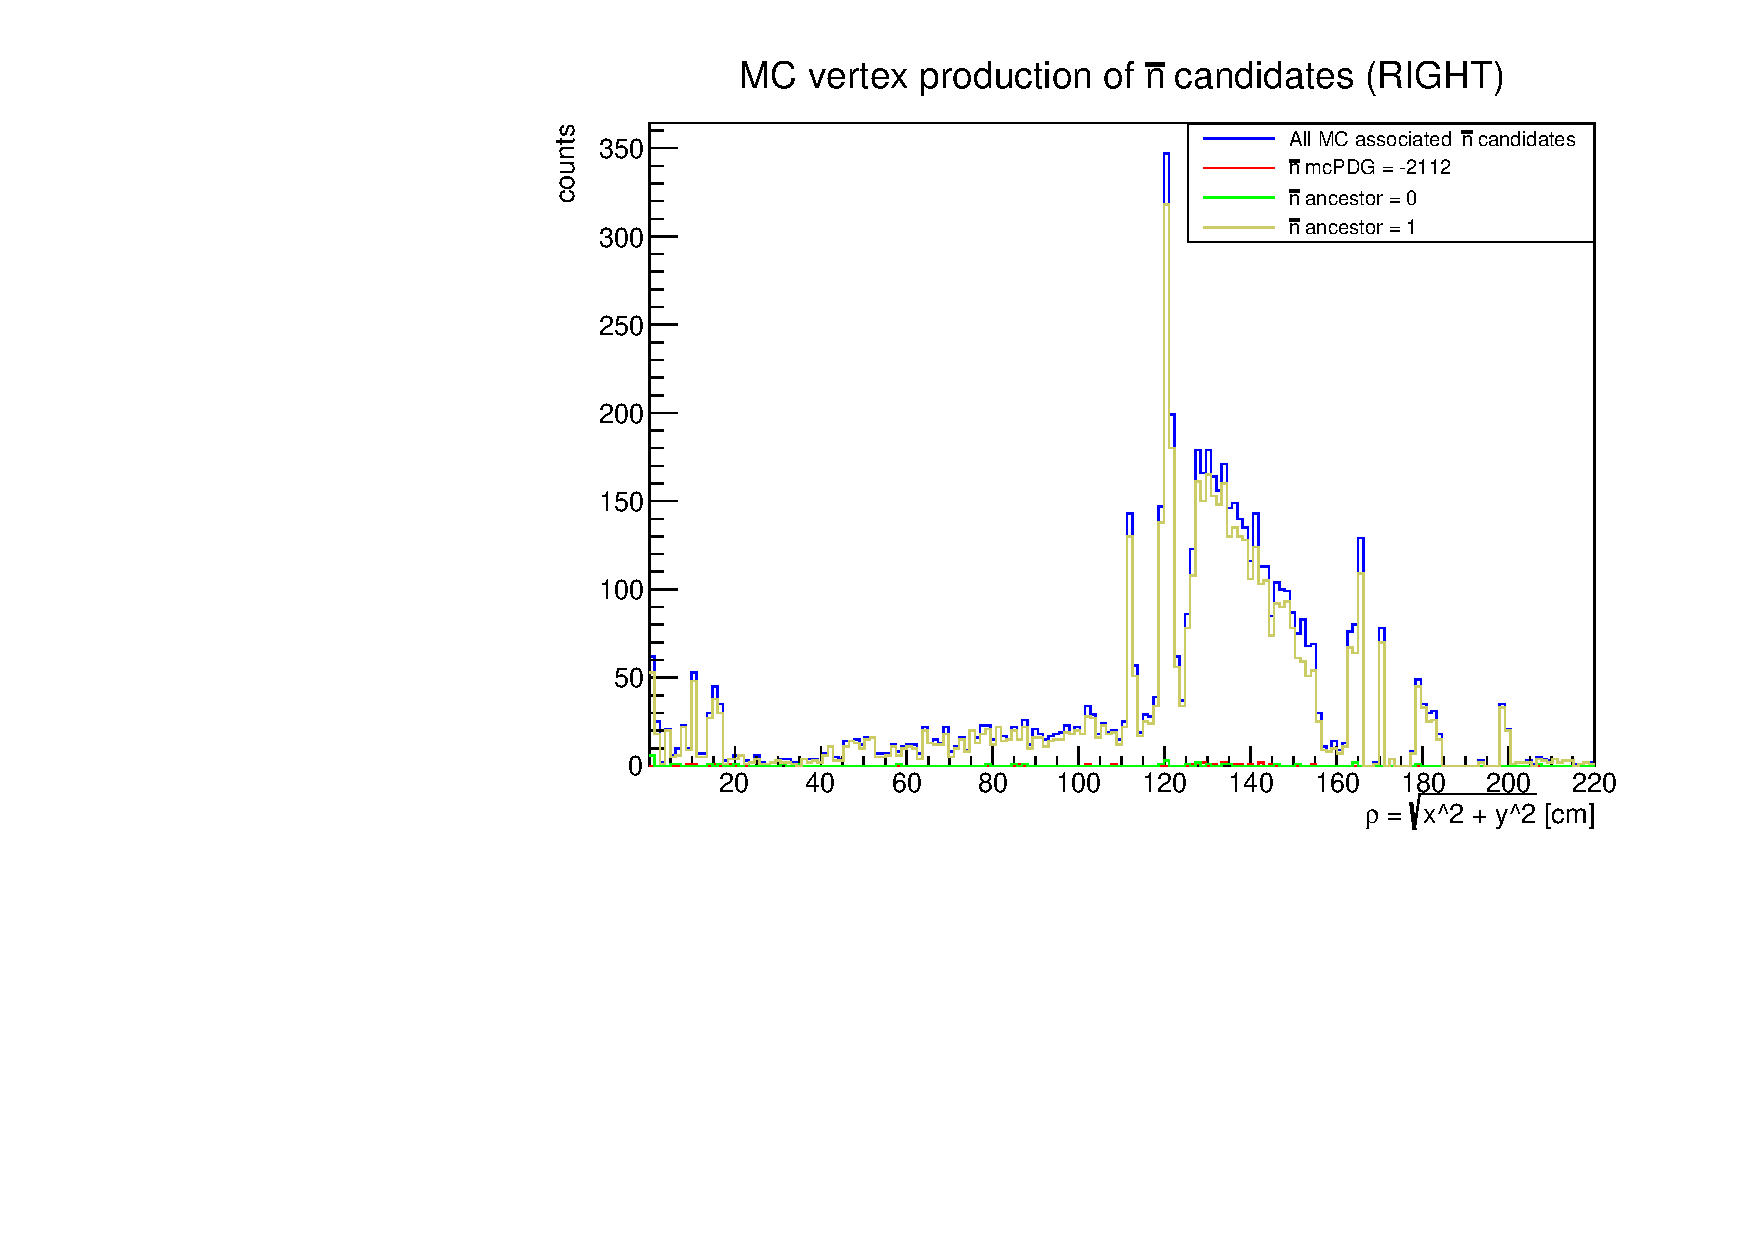
\includegraphics[width=0.49\textwidth]{nbar_MC/images/mcDistance_dx.pdf}
    \caption{$\bar{n}$ production vertex: (left) close to the IP (right) far from the IP}
\end{figure}

As expected, the correctly associated anti-neutrons ({\color{red} red distribution}) overlay the $\bar{n}$ candidates without an anti-neutron ancestor ({\color{green} green distribution}) and they are from the interaction point (left part). 
$\\$
As seen before, the $\bar{n}$ candidates with a $\bar{n}$ as mother are mainly photons and they are produced around the detector ({\color{yellow} yellow distribution}). It is interesting to note that the first structure is in the vertex detectors region ($\rho <$ 16 cm) and the two peaks located at the TOP edges, mainly around 118 cm (where the TOP begins) and 125 cm (where the TOP ends and the ECL starts), explicitly showing how cluster split-off and pre-showering events occur in the events.
$\\$
To compare the height comparison between the left and right contributes, the full distribution is shown below:
 \begin{figure}[H]
    \centering
    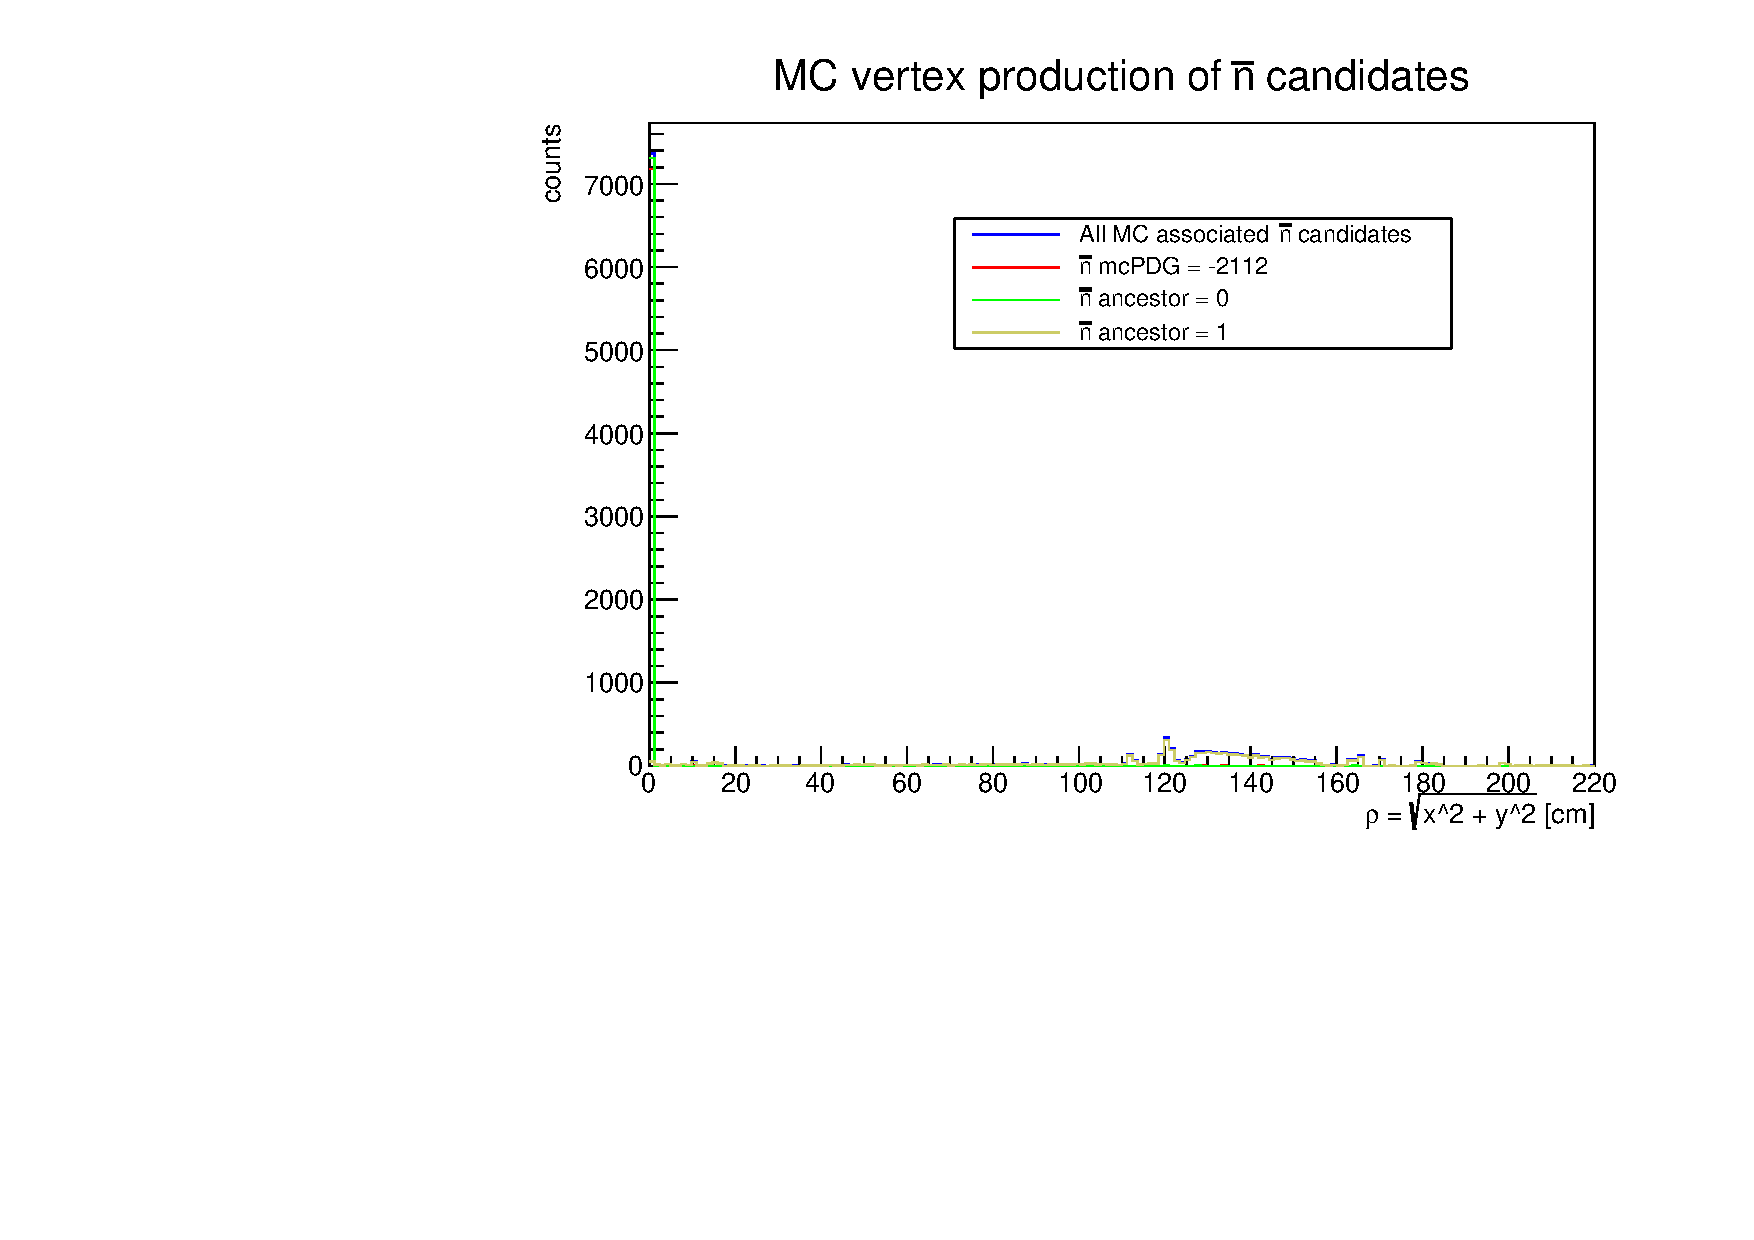
\includegraphics[width=0.70\textwidth]{nbar_MC/images/mcDistance_full.pdf}
     \caption{$\bar{n}$ production vertex showing the IP peak is the main one}
\end{figure}

\subsection{Kinematic Fit effects}
A \textbf{Kinematic Fit} is a constrained optimization technique used in particle physics to refine the measured four-momenta (or other kinematic quantities) of event particles by imposing known physical constraints, such as energy-momentum conservation or recoil mass. Measured quantities like track momenta, energies from calorimeters, or decay vertices come with resolution-limited errors from detectors. The fit adjusts these within their error bars to best satisfy the imposed constraint.
$\\$
There are several type of Kinematic Fit that could yield improved resolution. The one constraint \textbf{1C Kinematic Fit} has been tested over the $p \pi^- (\gamma_{ISR})$ system recoil mass, forcing it to the anti-neutron mass ($\sim 0.9385$ GeV) and then studying the response on the recoil kinematic variables resolution versus the anti-neutron candidate ones. The obtained residuals are shown below:

\begin{figure}[H]
    \centering
     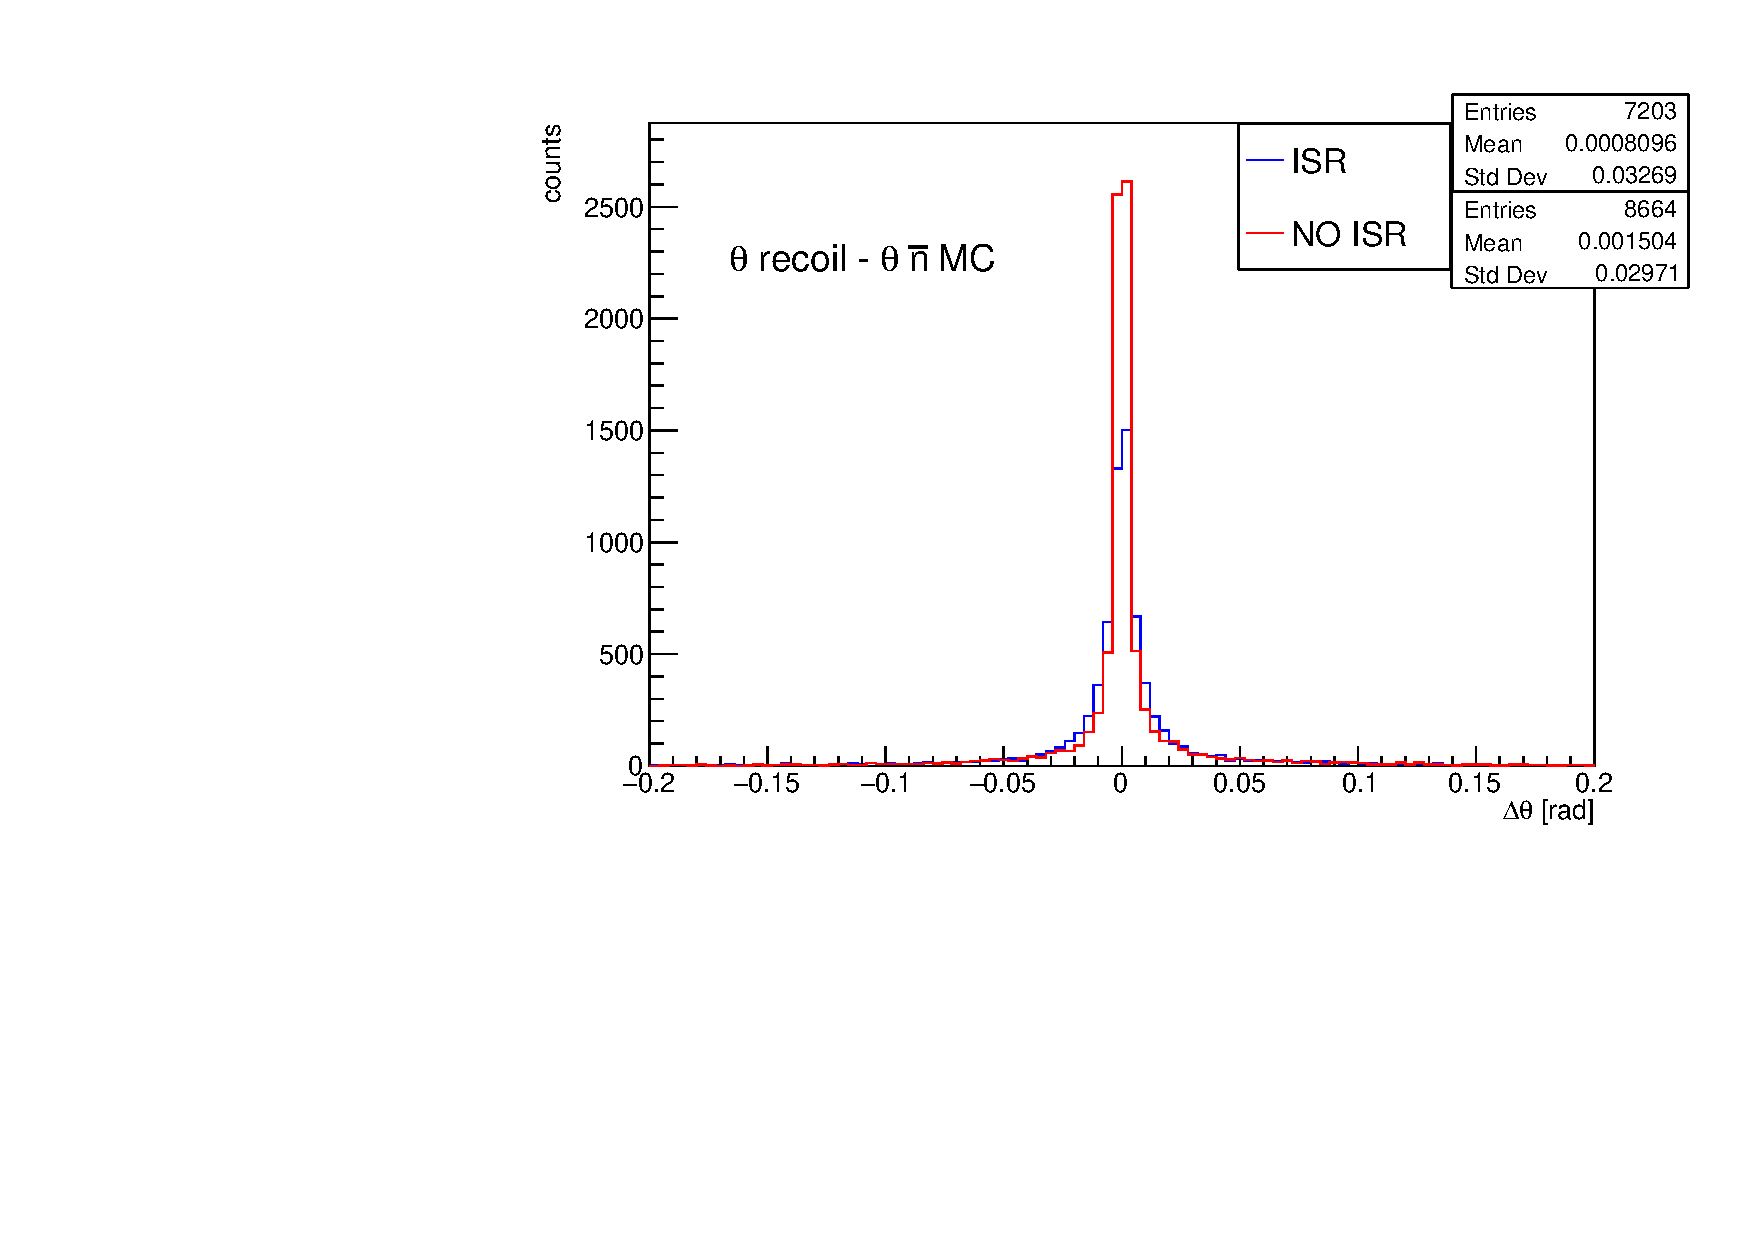
\includegraphics[width=0.49\textwidth]{nbar_MC/images/kin_delta_theta_mc.pdf}
     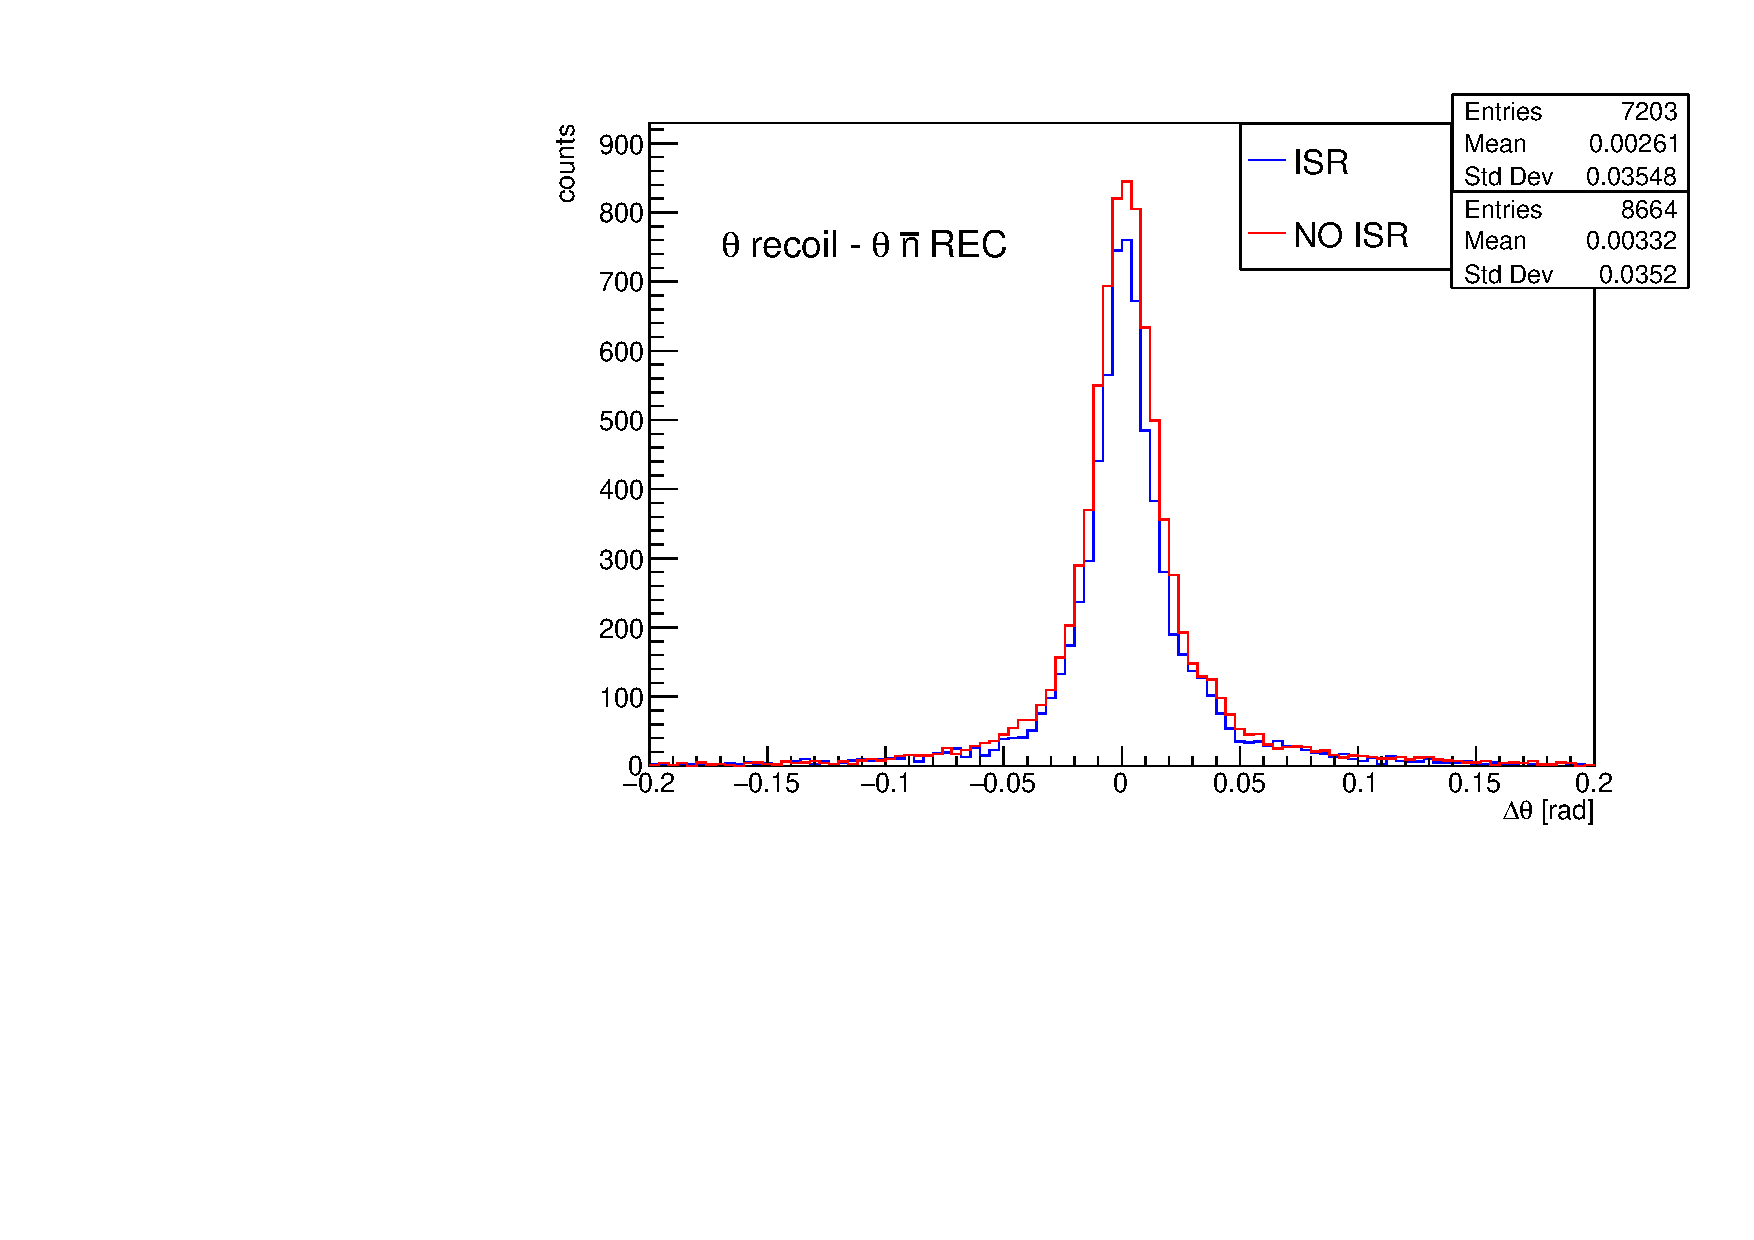
\includegraphics[width=0.49\textwidth]{nbar_MC/images/kin_delta_theta_rec.pdf}
     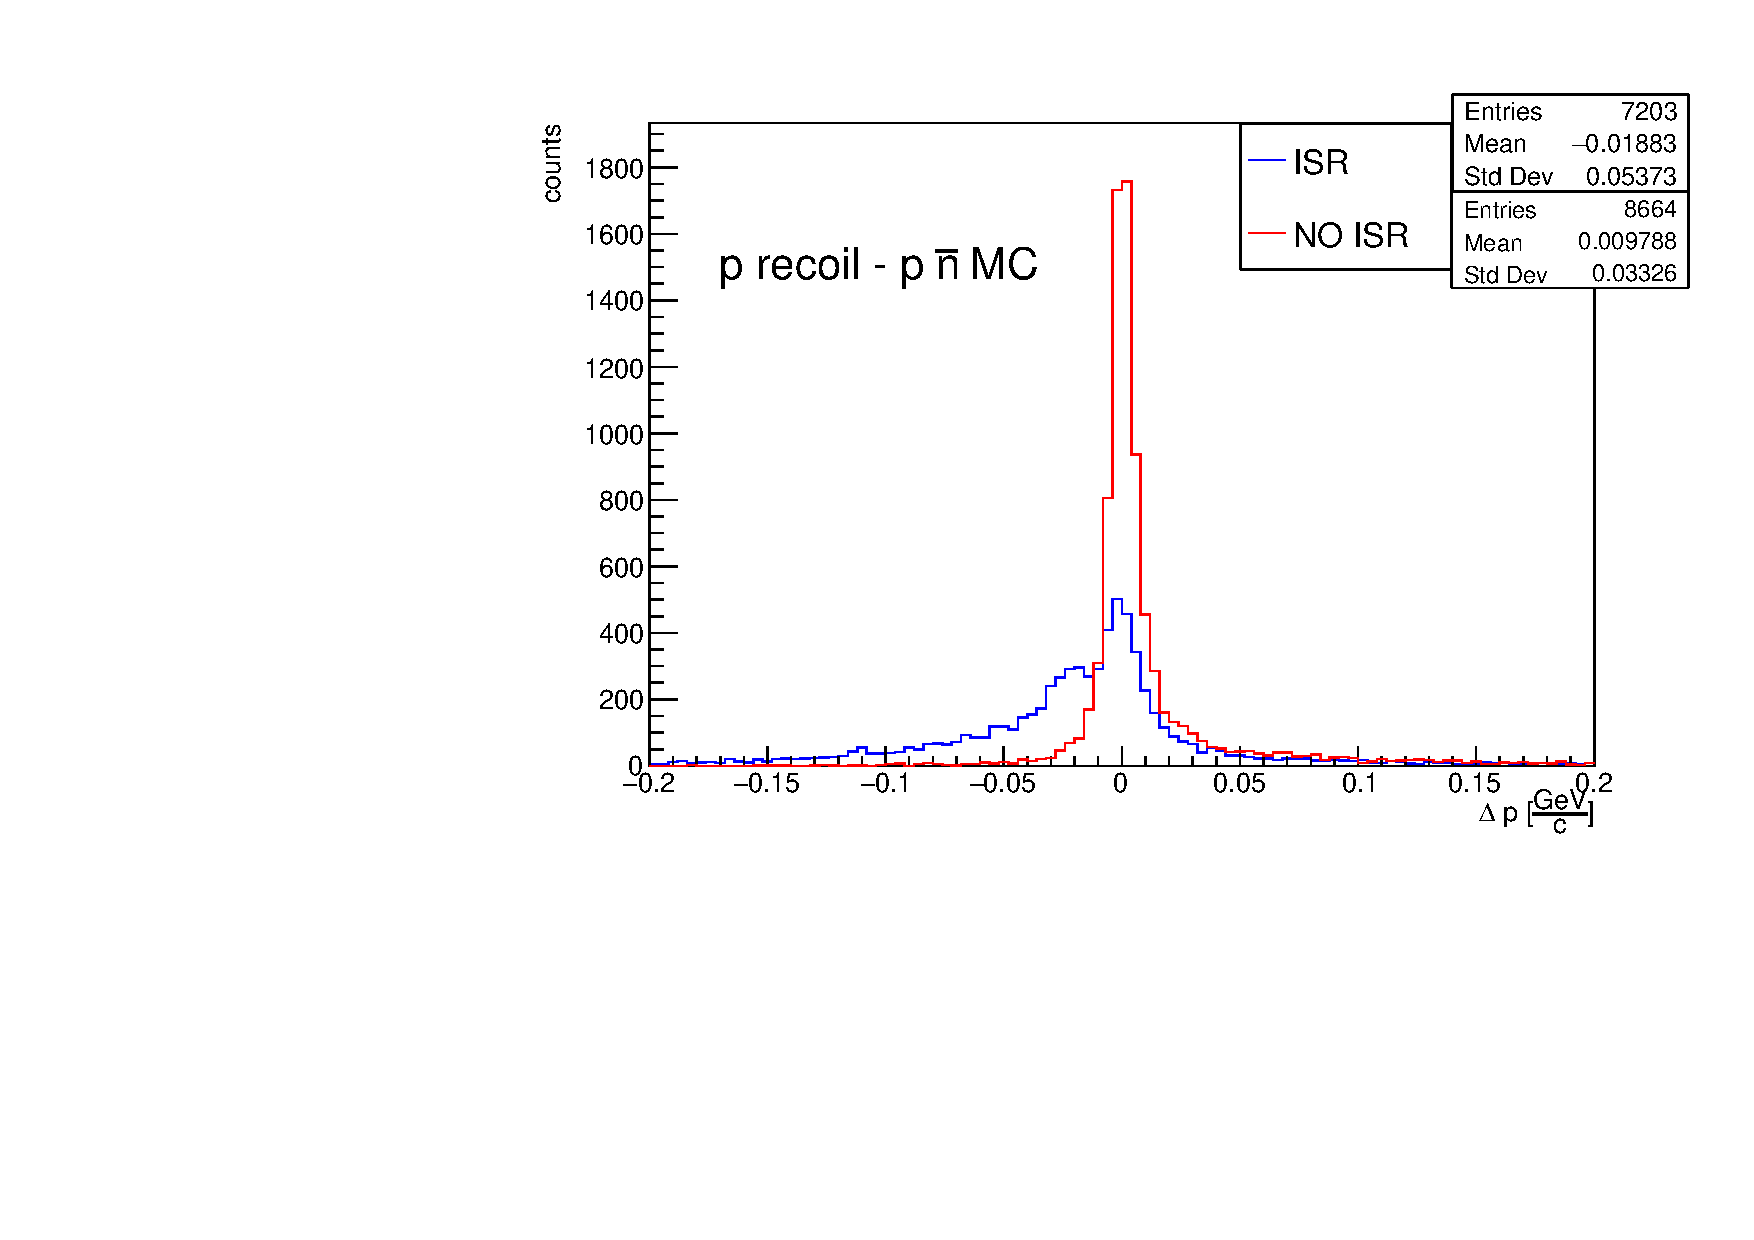
\includegraphics[width=0.49\textwidth]{nbar_MC/images/kin_delta_p_mc.pdf}
     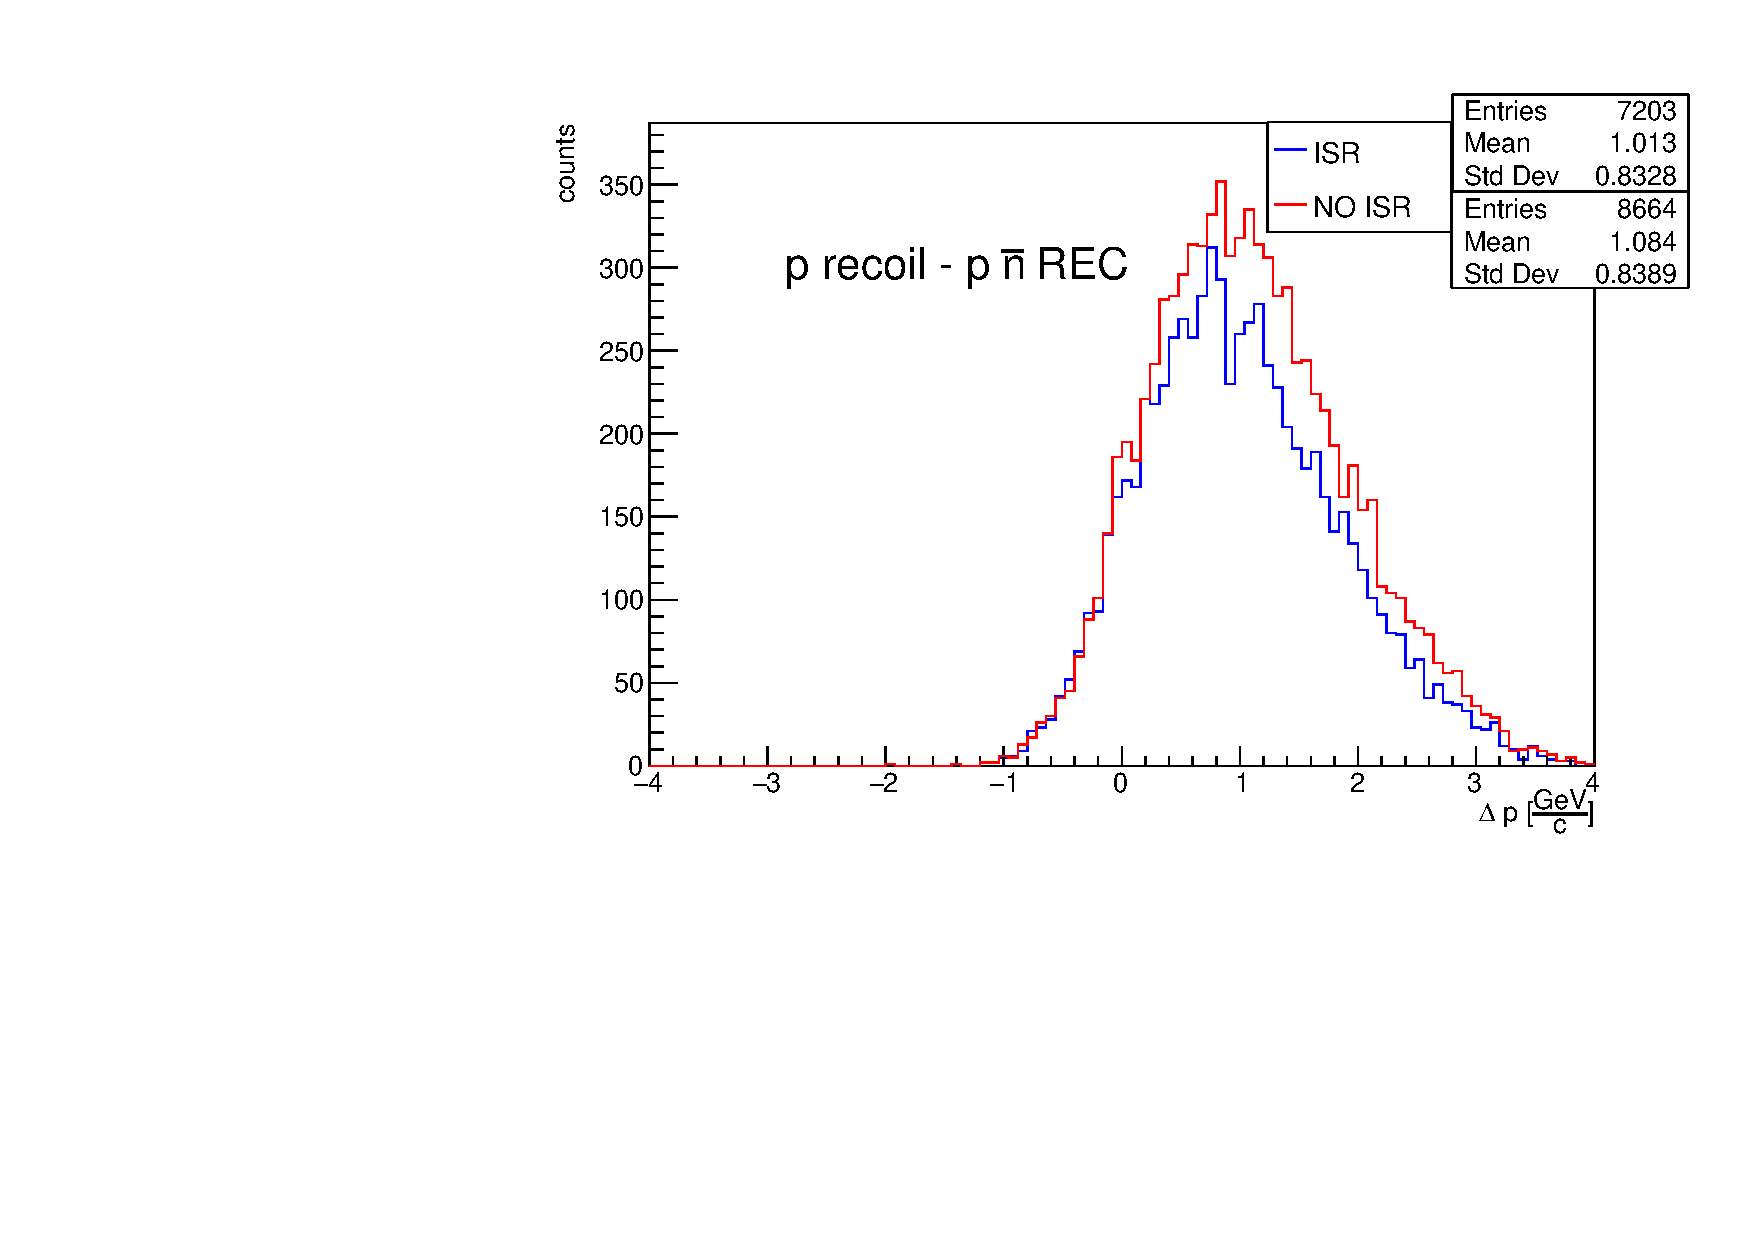
\includegraphics[width=0.49\textwidth]{nbar_MC/images/kin_delta_p_rec.pdf}
     \caption{Momentum and $\theta$ angle residuals distribution between recoil system and anti-neutron candidate, after the 1C Kinematic Fit procedure}
\end{figure}

As can be easily seen from the distributions, no significant improvement in recoil momentum resolution was observed post 1C Kinematic Fit compared to the unconstrained baseline ~\ref{fig:pRecoil-nP} . This confirms that the recoil system was already optimally reconstructed in the signal sample Monte Carlo. Further kinematic fit studies using a Monte Carlo cocktail are discussed in the next section.

\subsection{Shower shape variables in the signal sample}
The following chapter introduces the core of this thesis: the analysis of the \textbf{shower shape variables} of neutral ECL clusters associated with anti-neutron candidates. Since the final goal is to assess Data/MC agreement for these variables, the shower shape variables are first studied in an MC signal sample with no background channels present. The main idea is that particle identification can be achieved by studying the shower shapes and their characteristics.

\subsubsection{The analyzed shower shape variables}
The selected variables are the \textbf{cluster energy}, the \textbf{E1E9} variable, the \textbf{E9E21} variable, \textbf{Lateral Momentum}, \textbf{Second Moment}, \textbf{Zernike Moments} (50 and 41), and \textbf{Number of Hits}, which are described first. 

\paragraph{Cluster Energy}
$\\$
The Cluster Energy (\emph{clusterE} in the basf2 software), as the name suggests, represents the total energy deposited by the cluster associated with a given candidate particle, in this case the anti-neutron. It has units of GeV and only clusters with Cluster Energy above 20 MeV are stored by the reconstruction software.

\paragraph{Cluster E1E9 and E9E21}
In order to provide a proper definition of these variables (respectively \emph{clusterE1E9} and \emph{clusterE9E21} in the basf2 software), the following figure is shown below:

\begin{figure}[H]
    \centering
     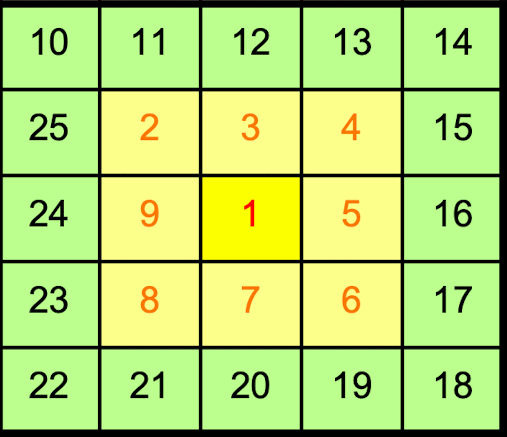
\includegraphics[width=0.50\textwidth]{nbar_MC/images/cluster}
     \caption{Ideal representation of a cluster pattern, consisting of a 5×5 matrix in which each cell corresponds to a single crystal}
\end{figure}

Cluster E1E9 and cluster E9E21 are defined as follow:

\begin{center}
$E1E9 = \frac{E_1}{\sum_{i=1}^{9} E_i}$ \hspace{0.2cm} $E9E21 = \frac{\sum_{j=1}^{9} E_j}{\sum_{j=10}^{25} E_j}$, with $j \ne 10,14,18,22$
\end{center}

The first one returns the ratio of the energy in the central crystal ($E_1$) to the total energy in the surrounding 3$\times$3 crystal grid ($E_9$). The second one returns the ratio of the energy in the 3x3 crystal grid around the central crystal ($E_1$) to the total energy in the 5$\times$5 crystal grid around the central crystal, excluding the corners. 
 $\\$
These ratios are always less than 1 and tend toward larger values for photons and smaller values for hadrons, as the latter produce more spread-out showers. These variables are dimensionless and are included within the range $[0,1]$.

\paragraph{Lateral Momentum}
$\\$
The cluster Lateral Momentum or Lateral Energy distribution (\emph{clusterLAT} in the basf2 software) is defined as follow:

\begin{center}
$C_{LM} = \frac{ \sum\limits_{i=2}^n E_i r_i^2} {  E_0 r_0^2 + E_1 r_0^2+ \sum\limits_{i=2}^n E_i r_i^2}$, 
\end{center}
with $r_0 \simeq 5$ cm (average distance between two crystals centres).  
$\\$
$n$ is the number of crystals associated to the shower, $E_i = (E_0,E_1,...)$  are the crystal energies sorted by descending energy and $r_i$ is the distance of the i-th digit to the shower center projected onto a plane perpendicular to the shower axis. For radially-symmetric electromagnetic showers, this variable peaks at $\sim 0.3$, where it is larger for hadronic particles. This variable is dimensionless and it is included within the range $[0,1]$.

\paragraph{Second Moment}
$\\$
The cluster Second Moment (\emph{clusterSecondMoment} in the basf2 software) is defined as follow:

\begin{center}
$C_{SM} = \frac{1}{S_0}\frac{ \sum\limits_{i=0}^n  E_i r_i^2} { \sum\limits_{i=0}^n E_i}$,
\end{center}
where $E_i$ and $r_i$ are the same variables as used for the lateral momentum, while $S_0$ is a normalization factor that normalizes to 1 for isolated photons, making $C_{SM}$ dimensionless. The Second Moment measures the dispersion of cluster size.

\paragraph{Zernike Moments}
$\\$
The Zernike Moments (Zernike Polynomials) are a set of orthogonal functions which are defined on the unit disk. Since each moment represents a specific pattern shape, they are widely used to represent smooth, two‑dimensional functions (especially wavefronts) over circular apertures. 
$\\$
On the unit disk parametrized by polar coordinates $(\rho,\phi)$ with $0 \le \rho \le 1$, the Zernike modes are usually written as:

   \begin{center}
	    $Z^{m}_n(\rho,\phi) = R^m_n(\rho)\,\cos(m\,\phi)$
	    
	    \vspace{0.3cm}
	    
	    $Z^{-m}_n(\rho,\phi) = R^m_n(\rho)\,\sin(m\,\phi)$	
     \end{center}  
    
Where:   
\begin{center}
 	$R^m_n(\rho) = \sum_{k=0}^{\tfrac{n-m}{2}} \frac{(-1)^k\,(n-k)!}{k!\left (\tfrac{n+m}{2}-k \right )! \left (\tfrac{n-m}{2}-k \right)!} \;\rho^{n-2\,k}$
 \end{center} 
 
$n$ represents the radial degree and $m$ represents the azimuthal frequency ($m = 0$ for spherical Zernike polynomials). A figure of the Zernike polynomials is given below:
\begin{figure}[H]
    \centering
     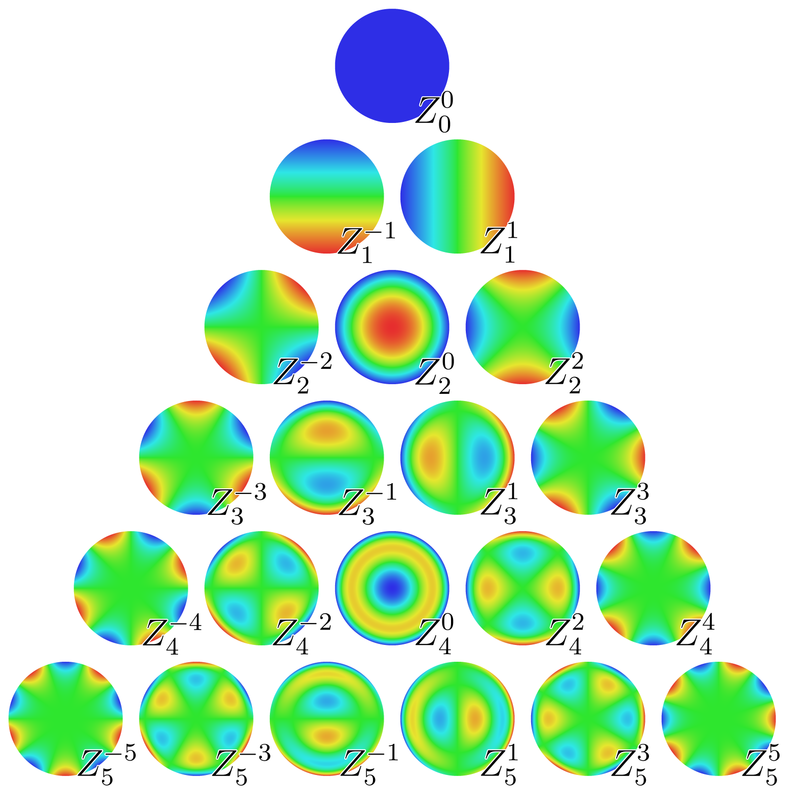
\includegraphics[width=0.60\textwidth]{nbar_MC/images/zernike}
     \caption{Zernike Polynomials representation. Moments $Z^0_4$ and $Z^1_5$ are widely discussed in this thesis}
\end{figure}

Precisely, Zernike Moments  $Z^0_4$ and $Z^1_5$ (\emph{clusterAbsZernikeMomen40} and \emph{clusterAbsZernikeMoment51} in the basf2 software) are studied in this thesis, where the first one represents the radial spread distribution structure, while the second one represents the level of dipolar asymmetry.

\paragraph{Number of Crystals hit}
$\\$
The variable Number of Crystals hit (\emph{clusterNhits} in the basf2 software) returns sum of weights $w_i$, with $w_i \le 1$ of all crystals in the cluster. For non-overlapping clusters this is equal to the number of crystals in the cluster. However, in the case of overlapping clusters where individual crystal energies are split among them, this can be a non-integer value.

\subsubsection{Anti-neutrons ECL cluster variables}
In order to isolate the contribution of the neutral clusters which are correctly associated with $\bar{n}$ particles (Monte Carlo PDG = -2112) ({\color{red} red distribution}) from all $\bar{n}$ candidates ({\color{blue} blue distribution}), the two distributions are overlaid for each cluster variable. The former is naturally included within the latter, naturally.
\newpage
The obtained cluster variables in ISR case are shown below:
 \begin{figure}[H]
    \centering
    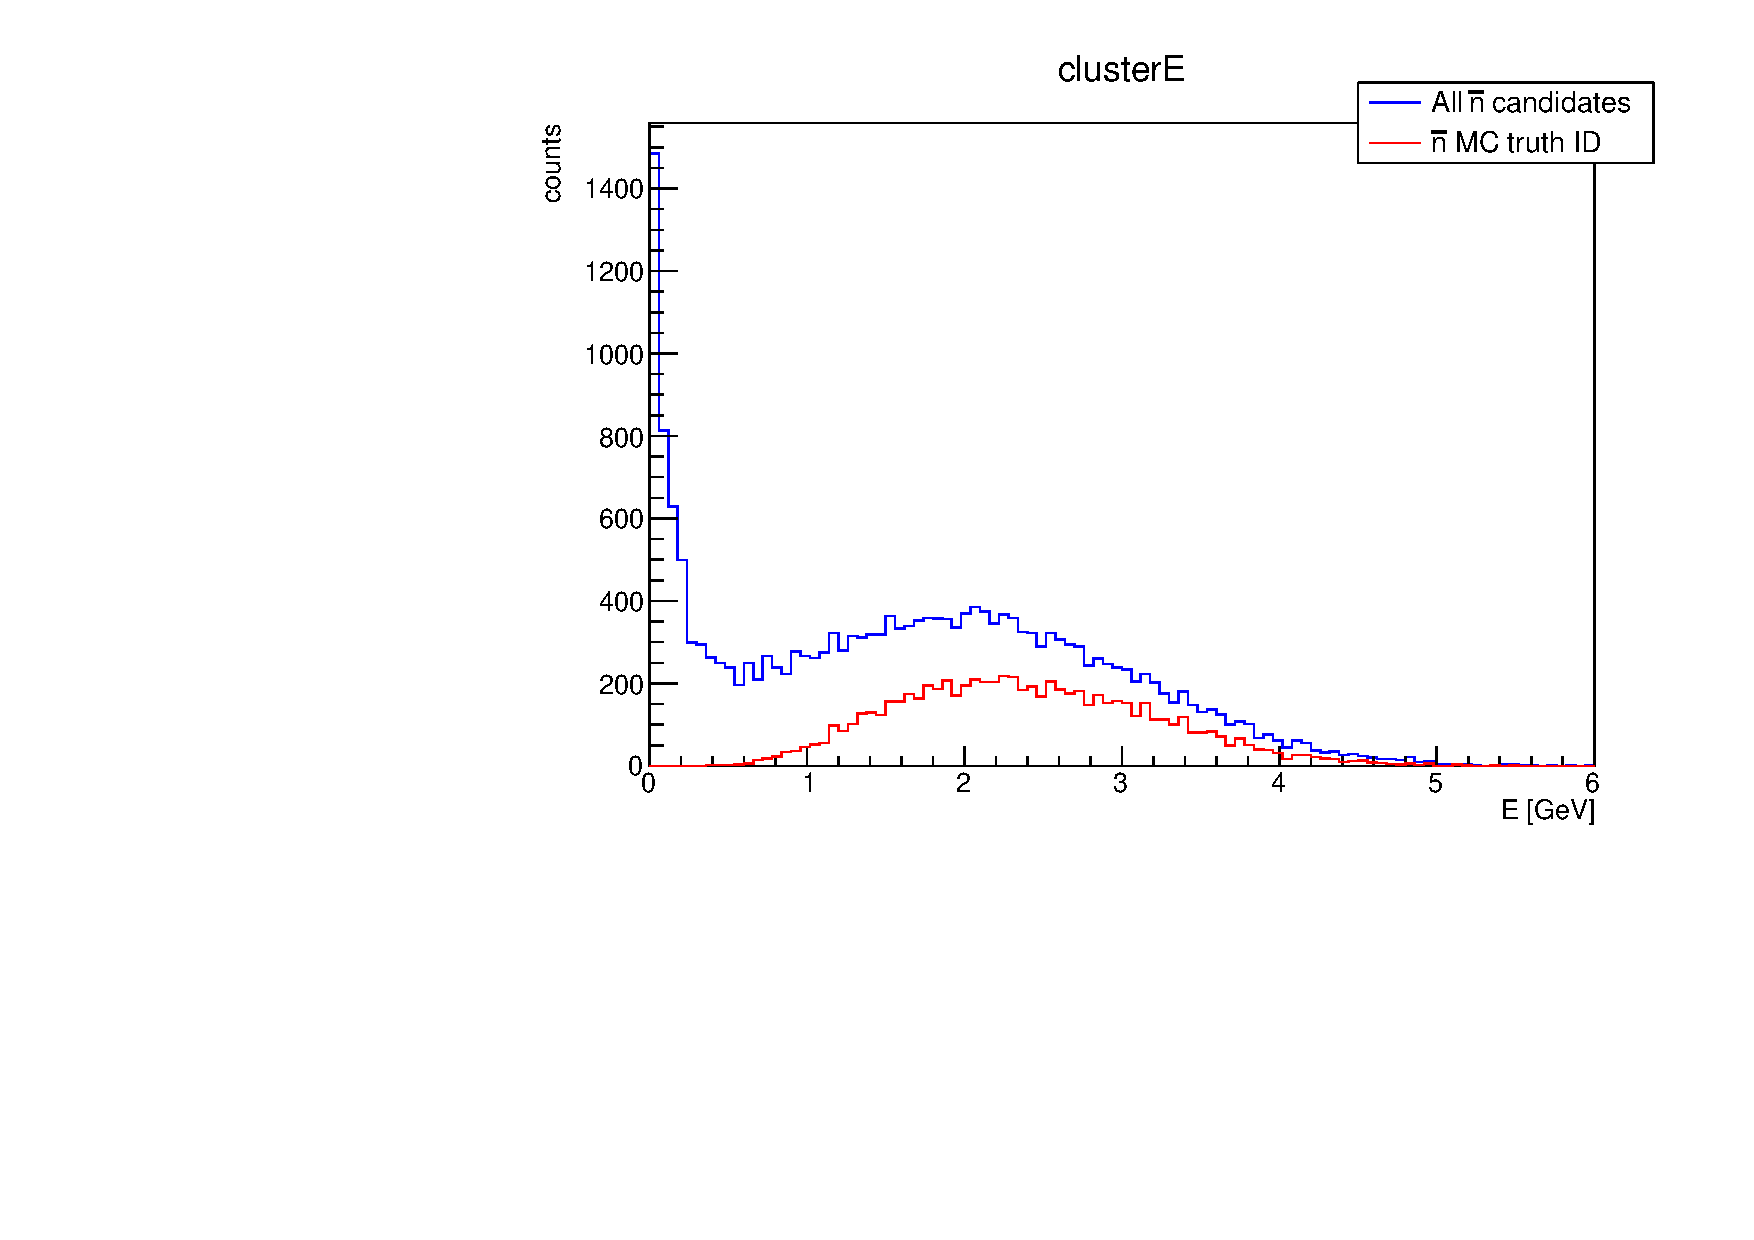
\includegraphics[width=0.49\textwidth]{nbar_MC/images/clusterE_isr.pdf}
    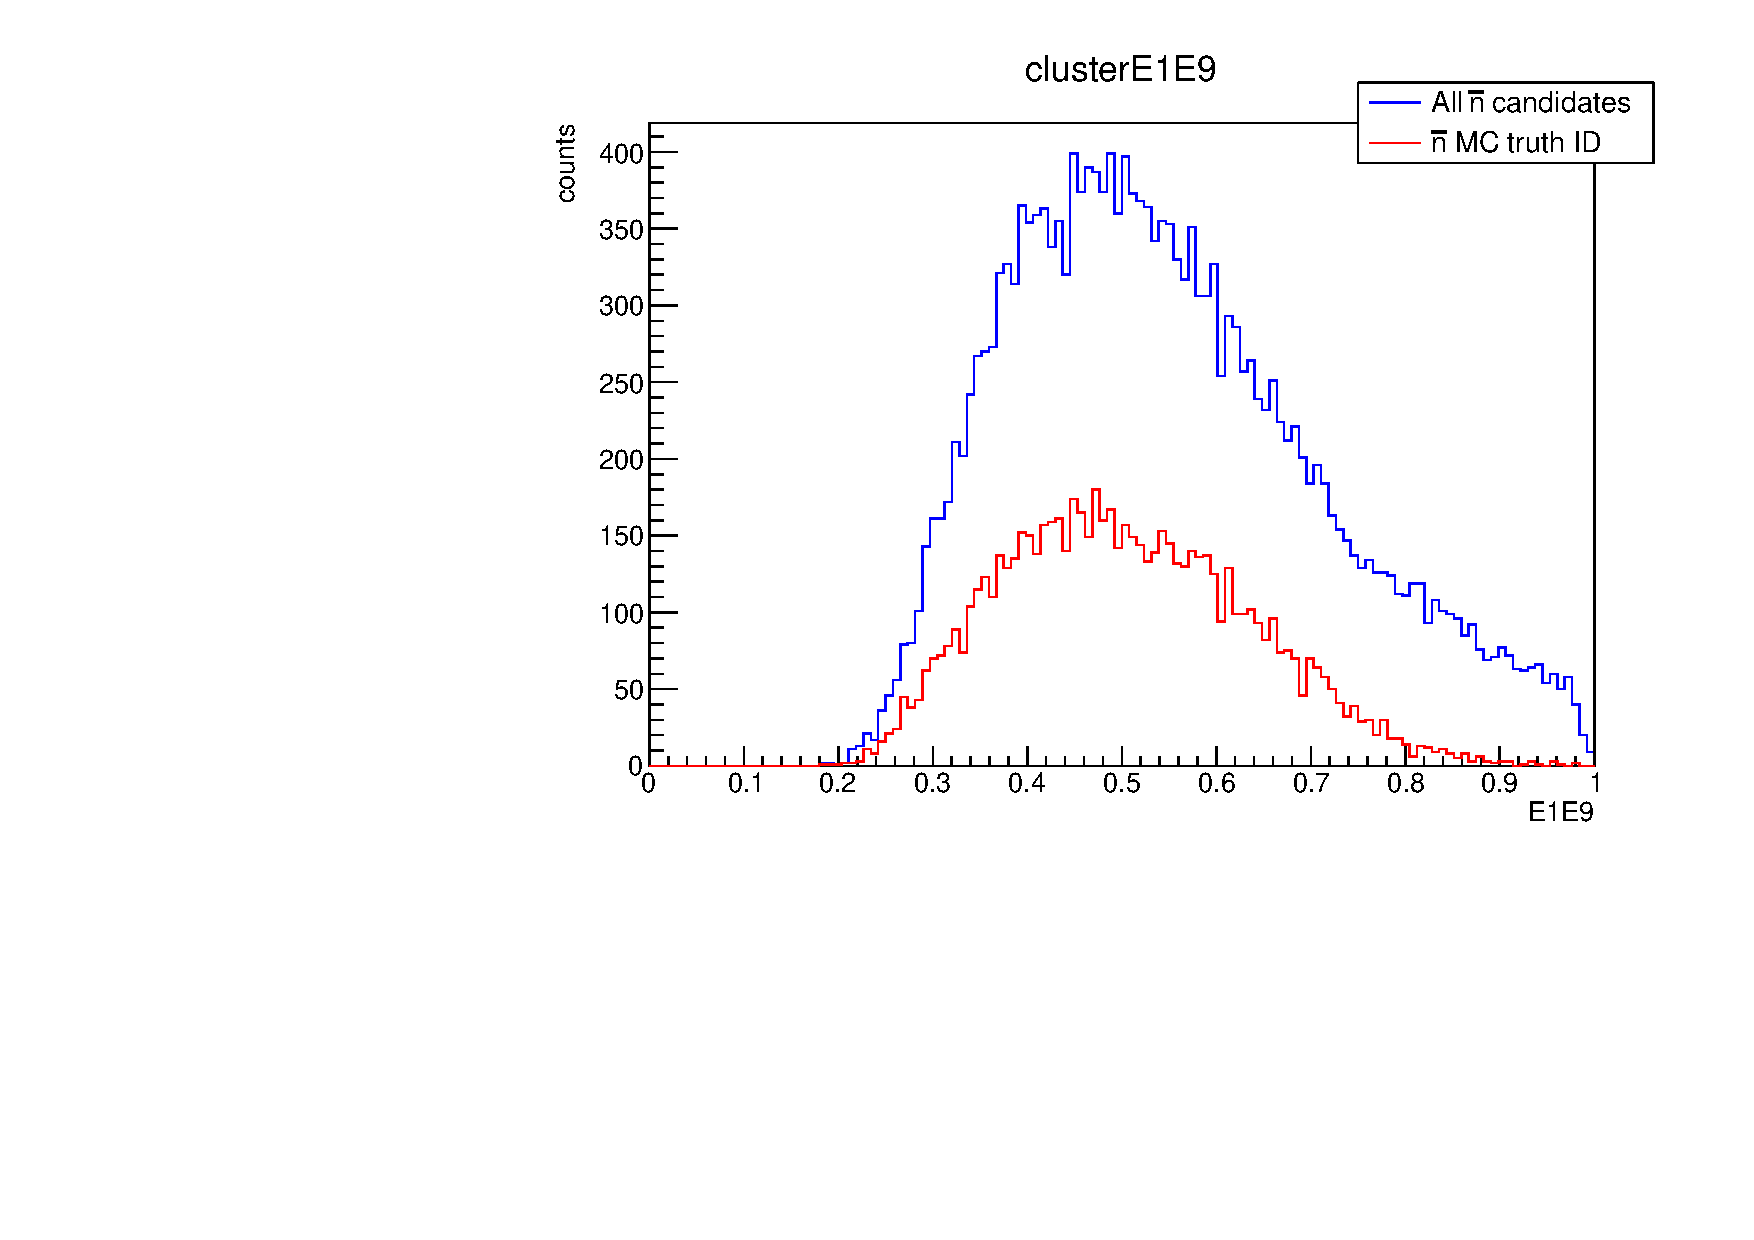
\includegraphics[width=0.49\textwidth]{nbar_MC/images/clusterE1E9_isr.pdf}
    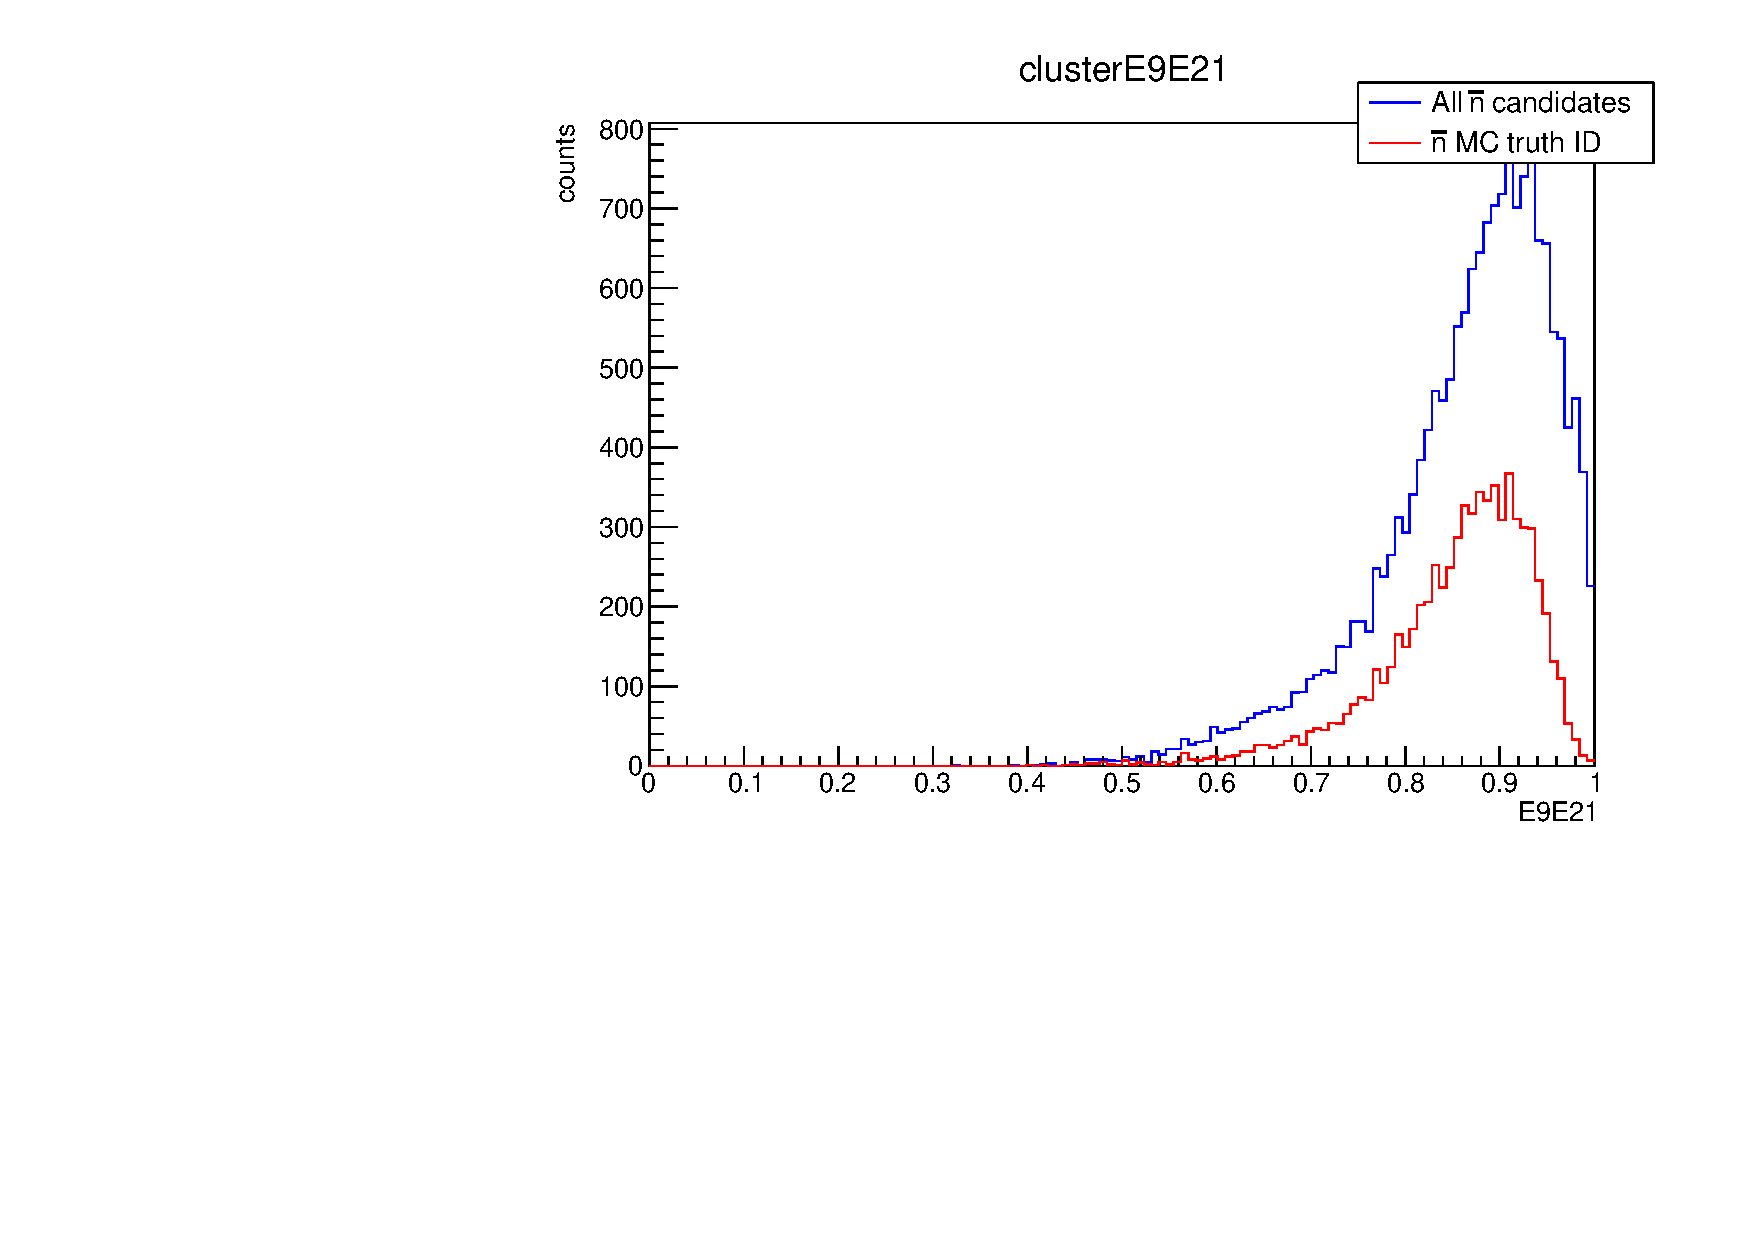
\includegraphics[width=0.49\textwidth]{nbar_MC/images/clusterE9E21_isr.pdf}
    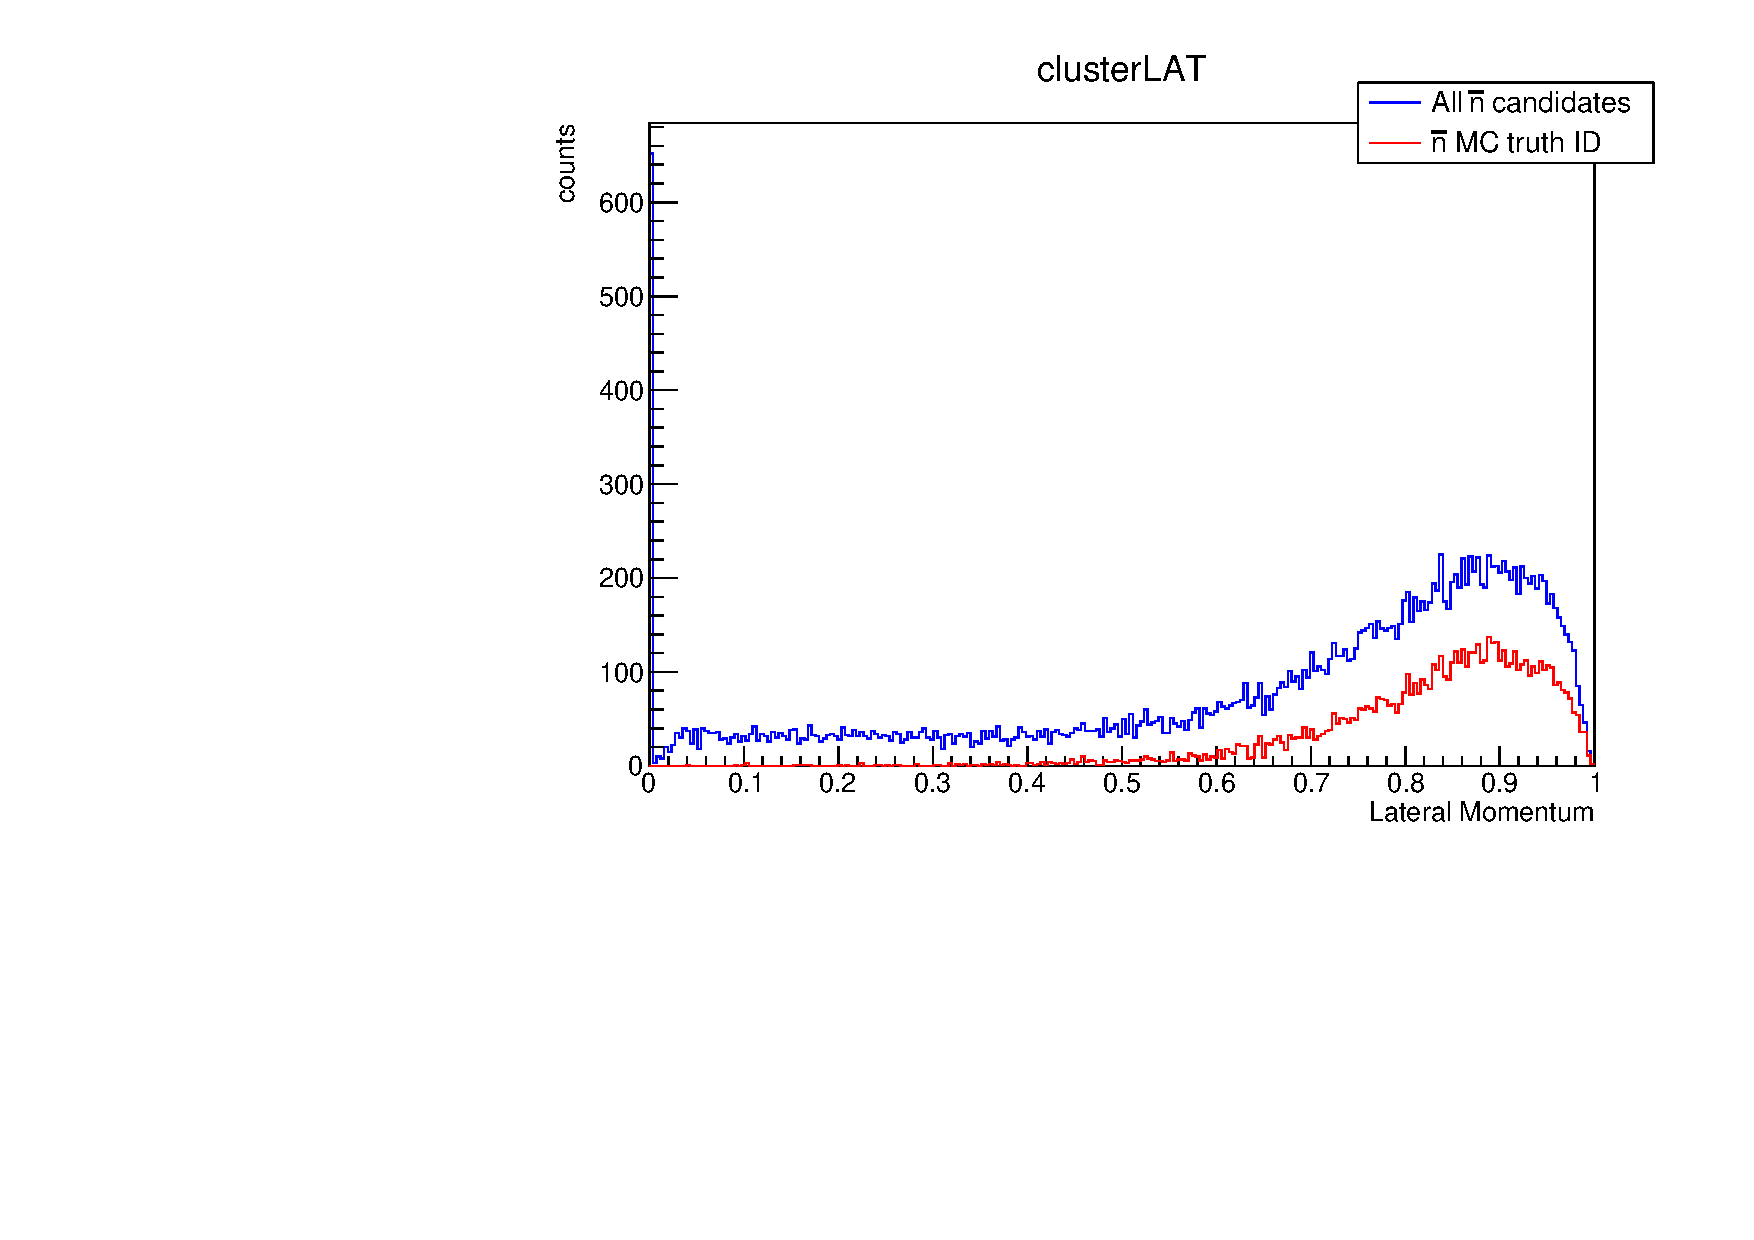
\includegraphics[width=0.49\textwidth]{nbar_MC/images/clusterLAT_isr.pdf}
    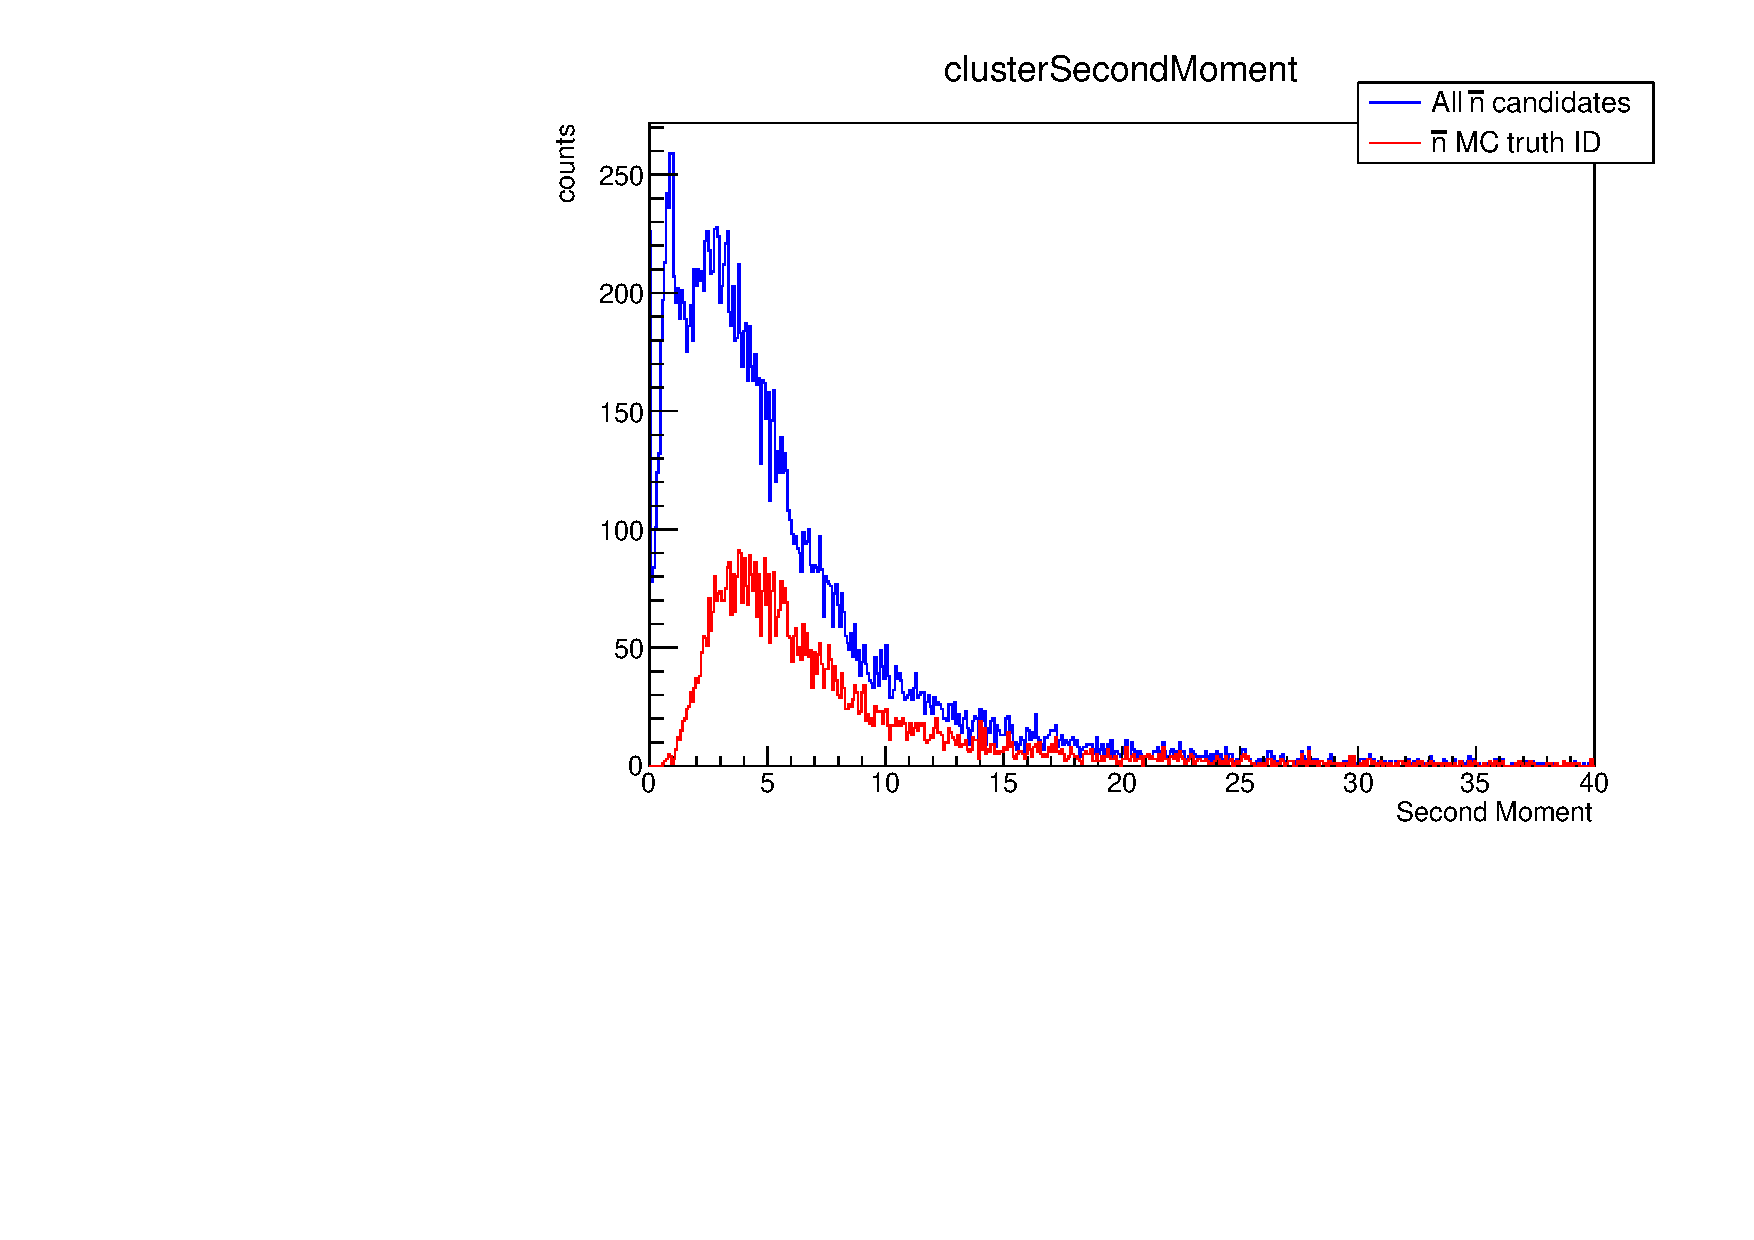
\includegraphics[width=0.49\textwidth]{nbar_MC/images/clusterSecondMoment_isr.pdf}
    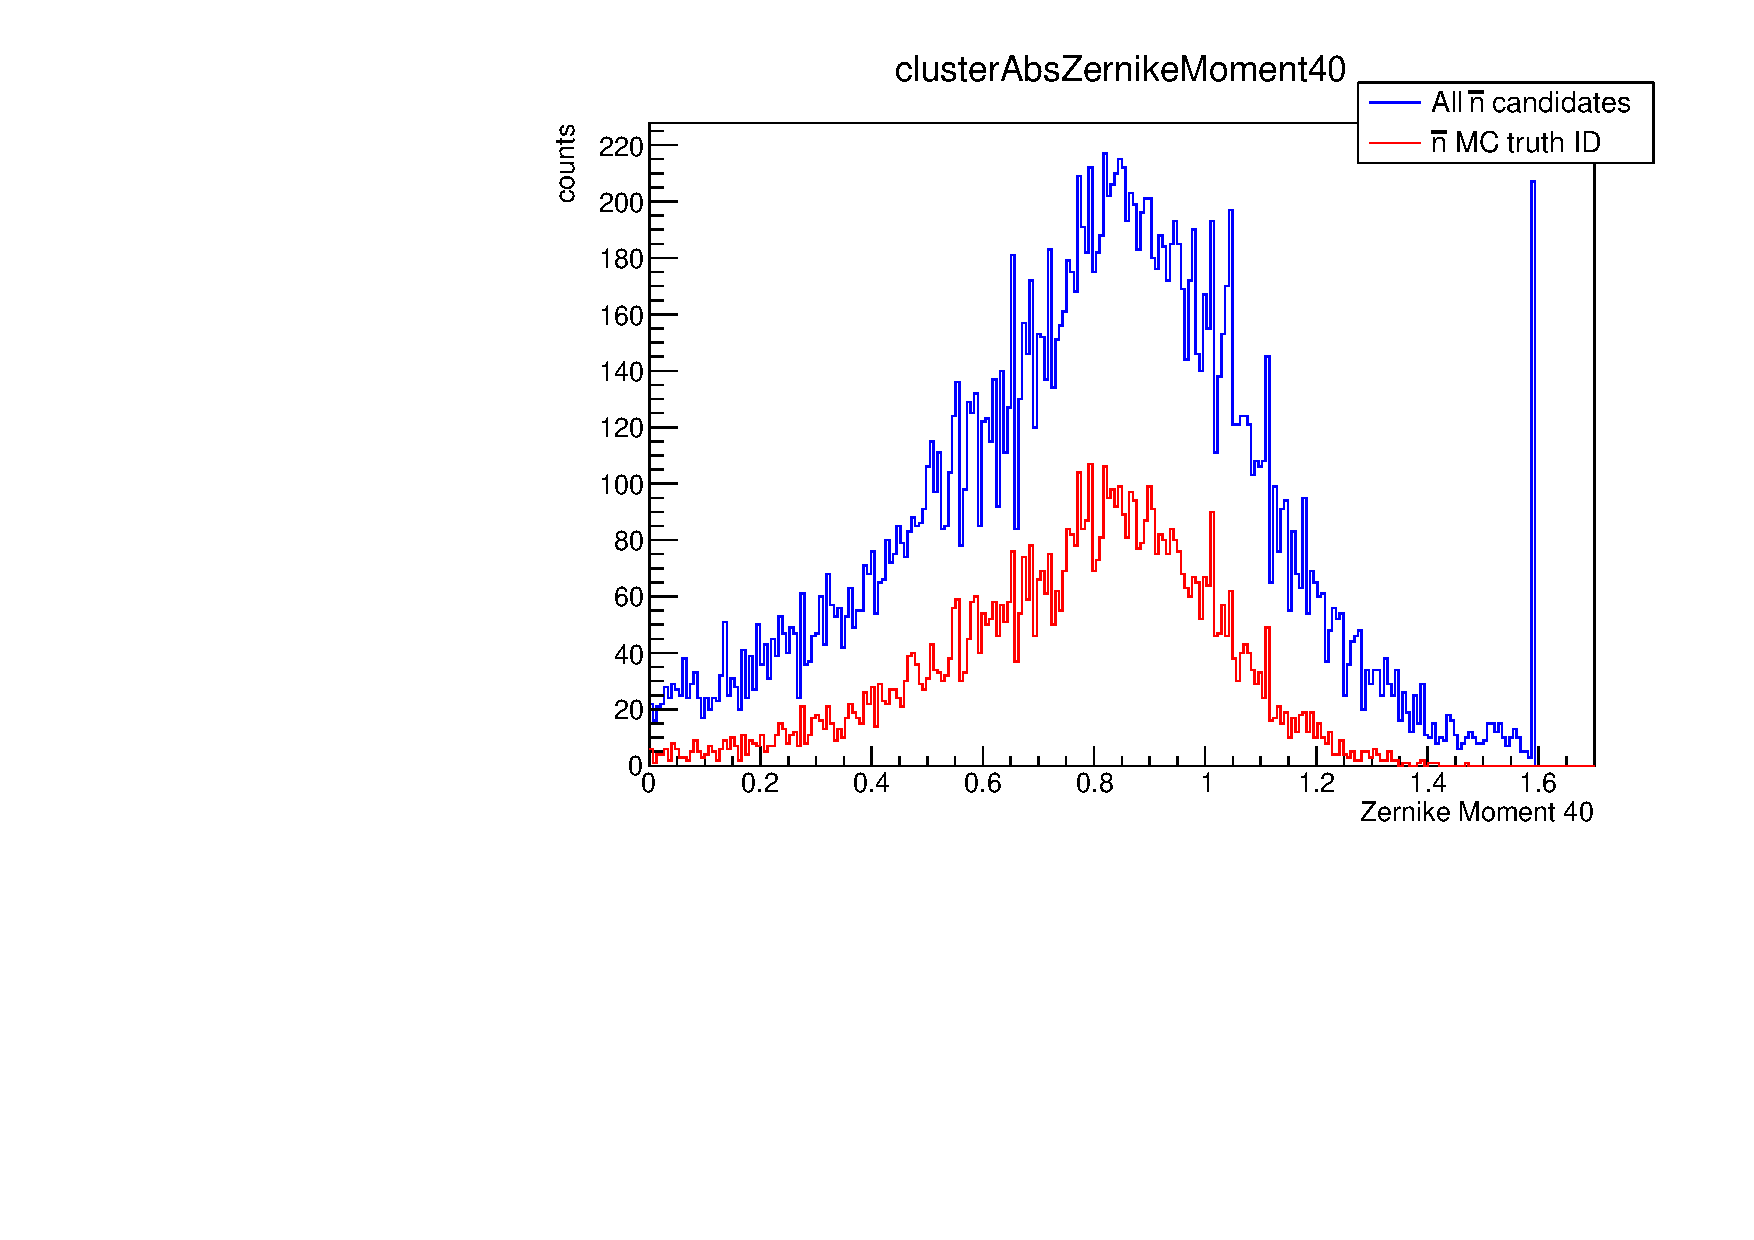
\includegraphics[width=0.49\textwidth]{nbar_MC/images/clusterAbsZernikeMoment40_isr.pdf}
    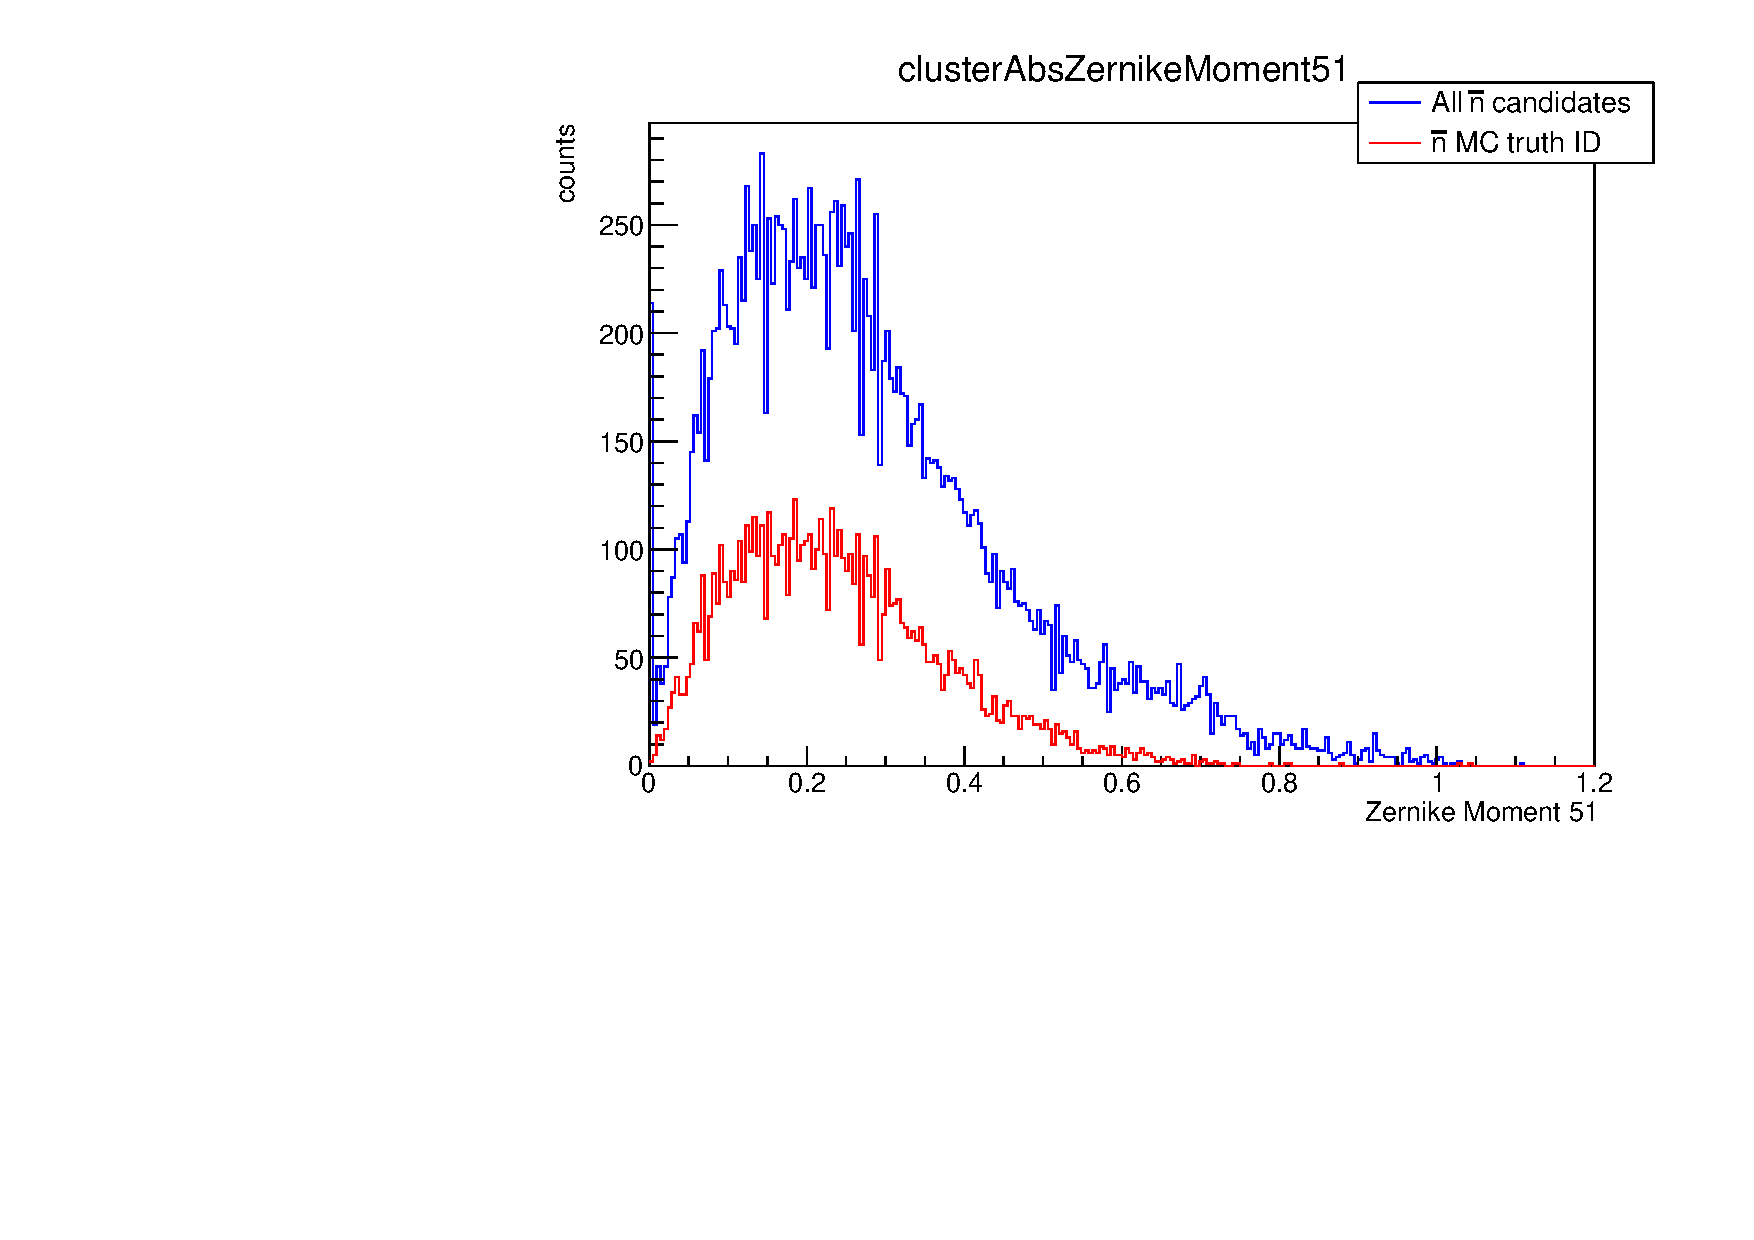
\includegraphics[width=0.49\textwidth]{nbar_MC/images/clusterAbsZernikeMoment51_isr.pdf}
    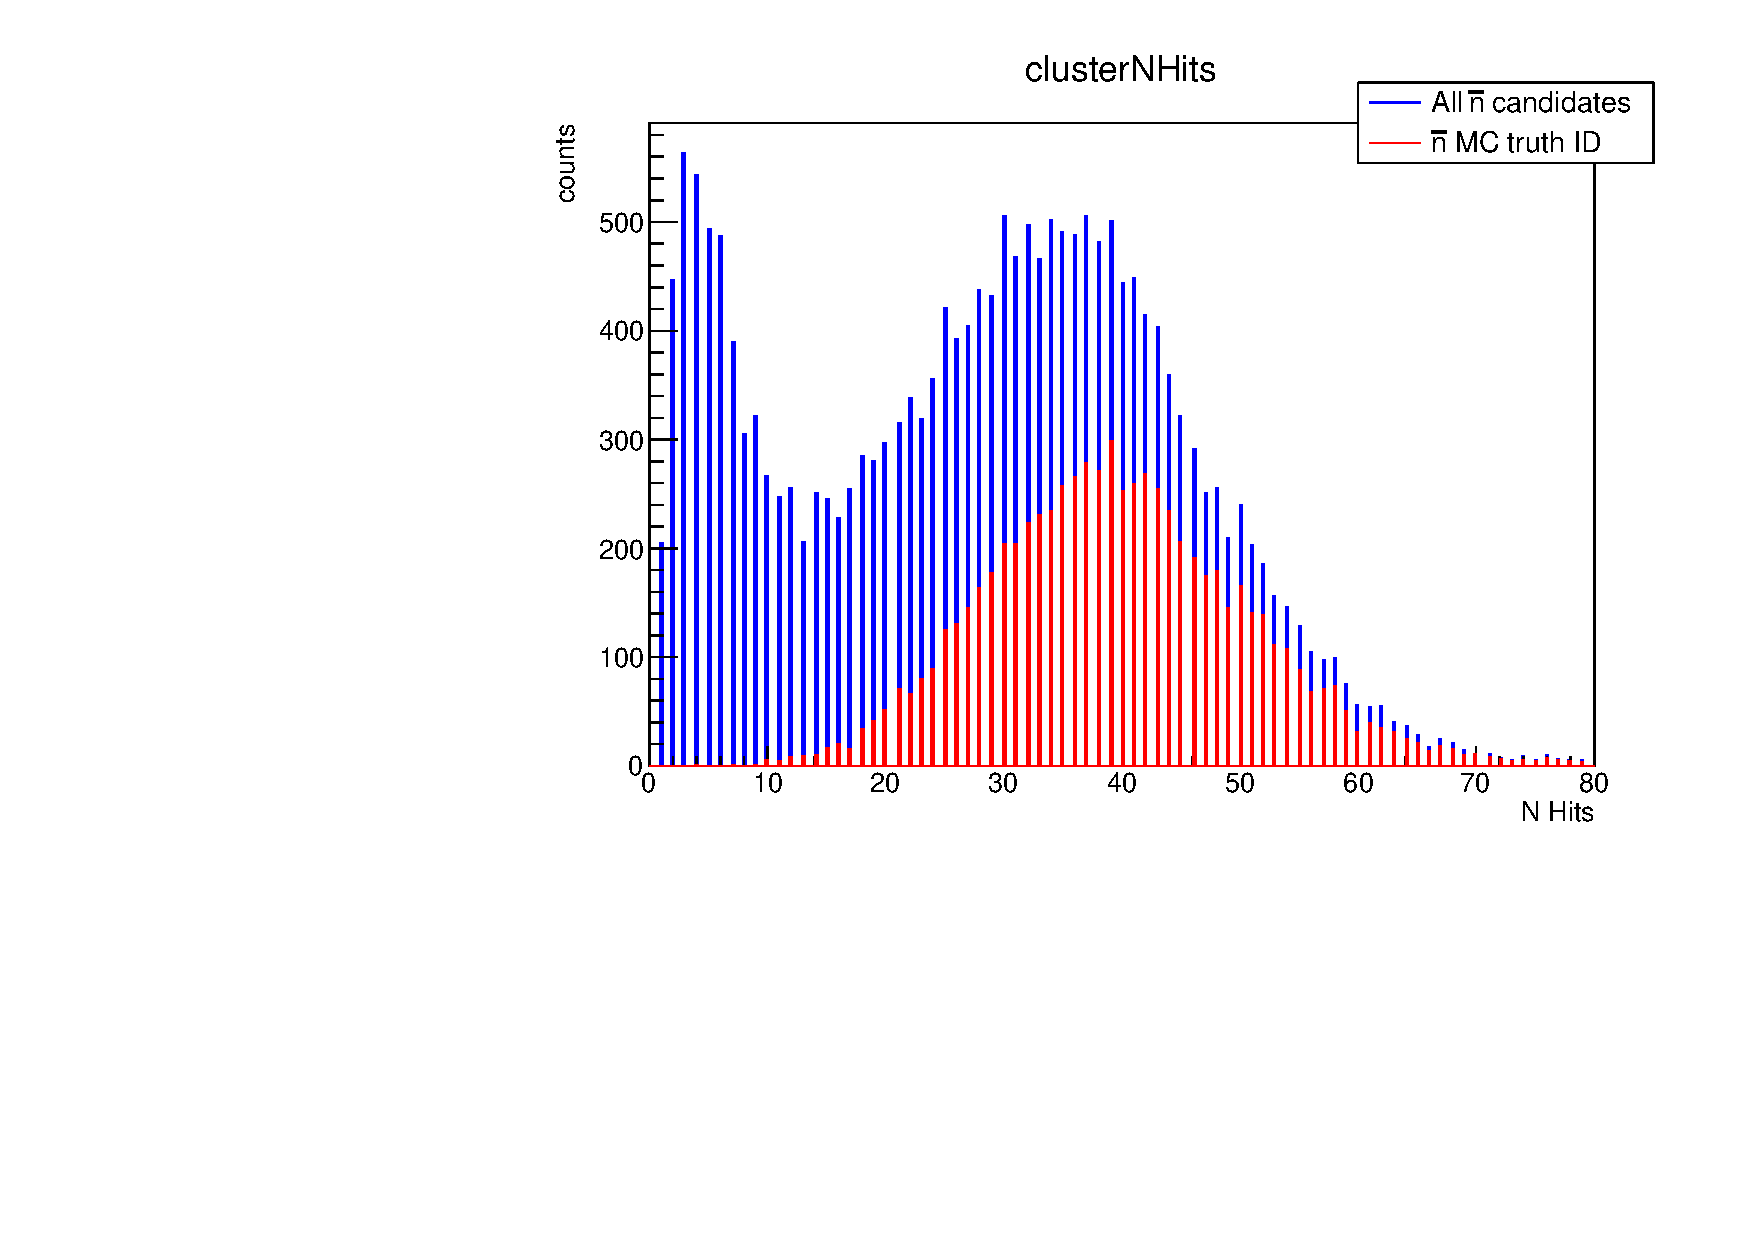
\includegraphics[width=0.49\textwidth]{nbar_MC/images/clusterNHits_isr.pdf}
   
     \caption{Comparison of reconstructed cluster variables for all $\bar{n}$ candidates versus those associated with $\bar{n}$ particles by Monte Carlo truth Monte Carlo PDG = -2112 (ISR case). The selection is performed using the Monte Carlo PDG code ($-2112$), as previously discussed}

\end{figure}

\newpage
The obtained cluster variables in NO ISR case are shown below:
 \begin{figure}[H]
    \centering
    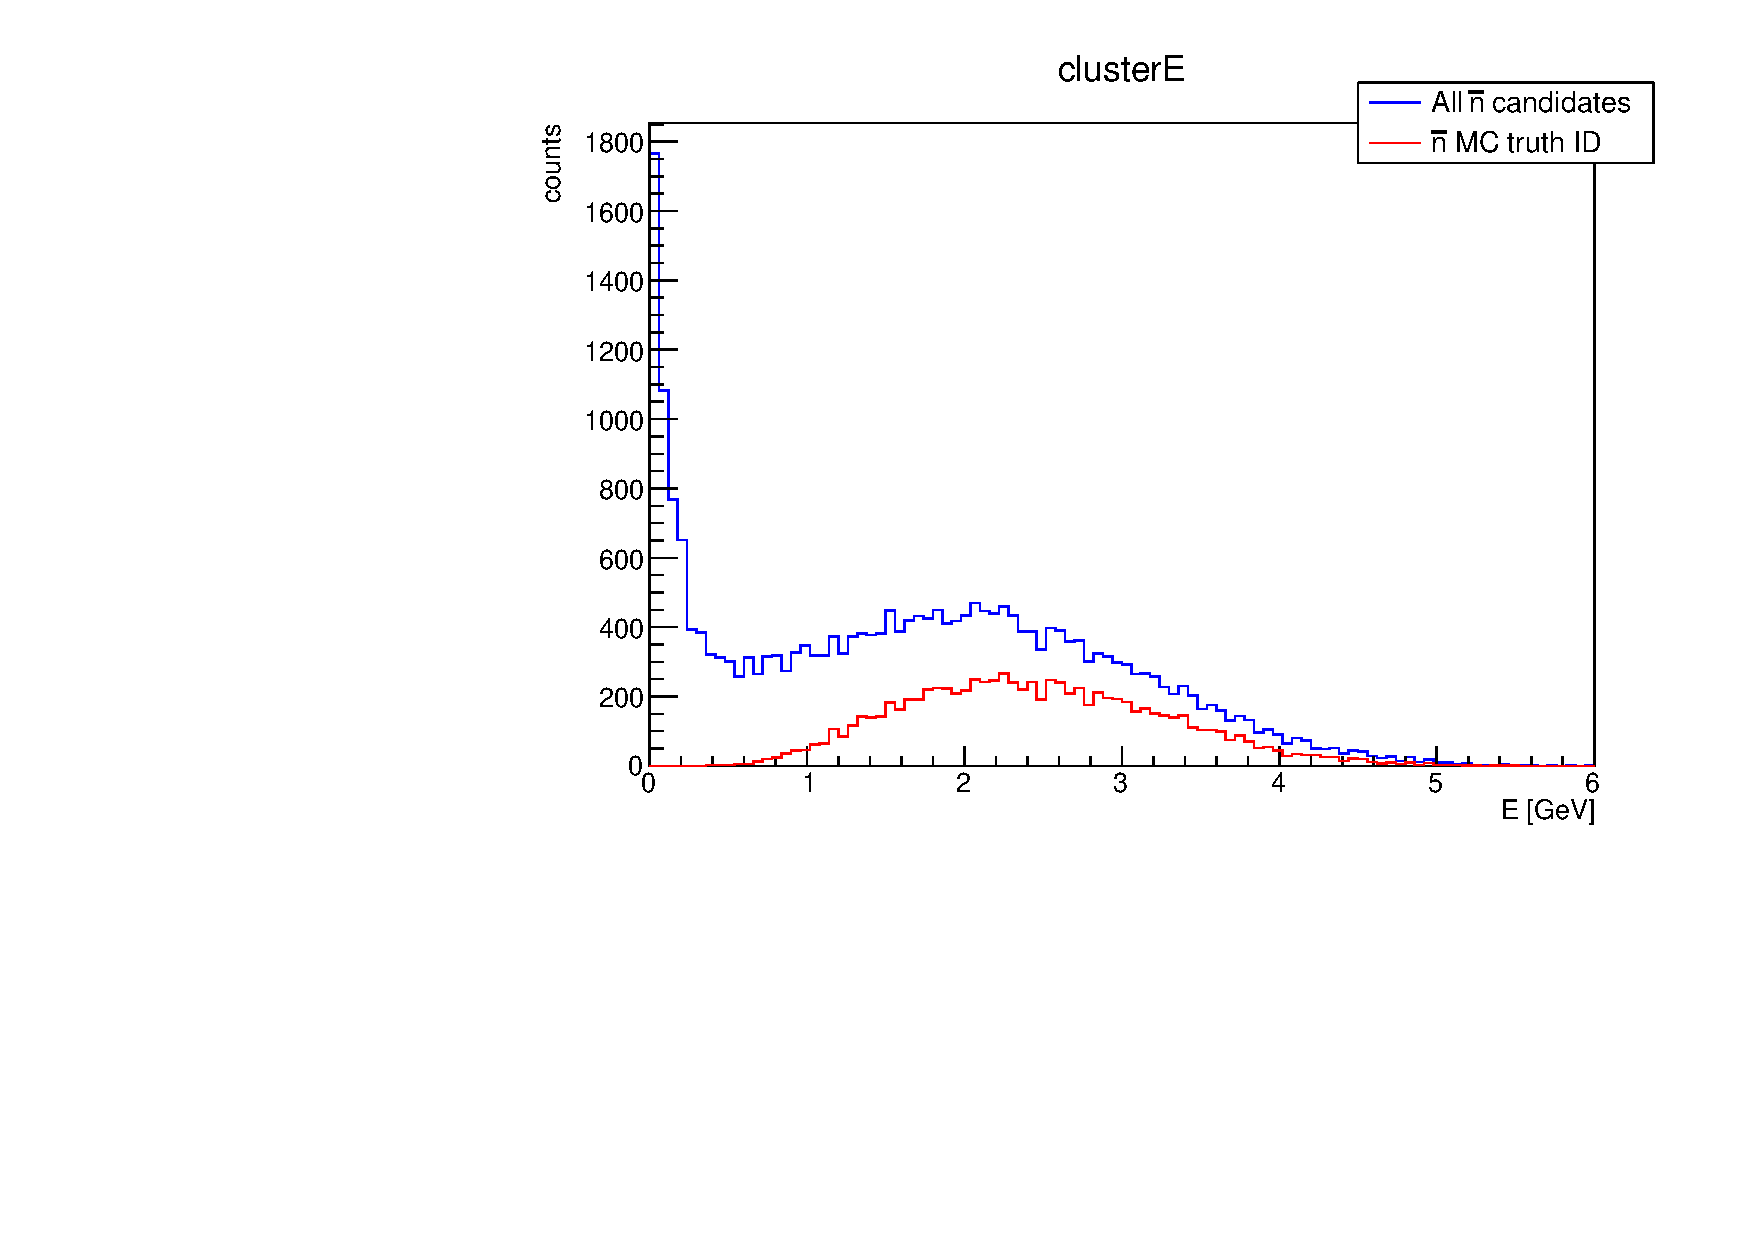
\includegraphics[width=0.49\textwidth]{nbar_MC/images/clusterE_nog.pdf}
    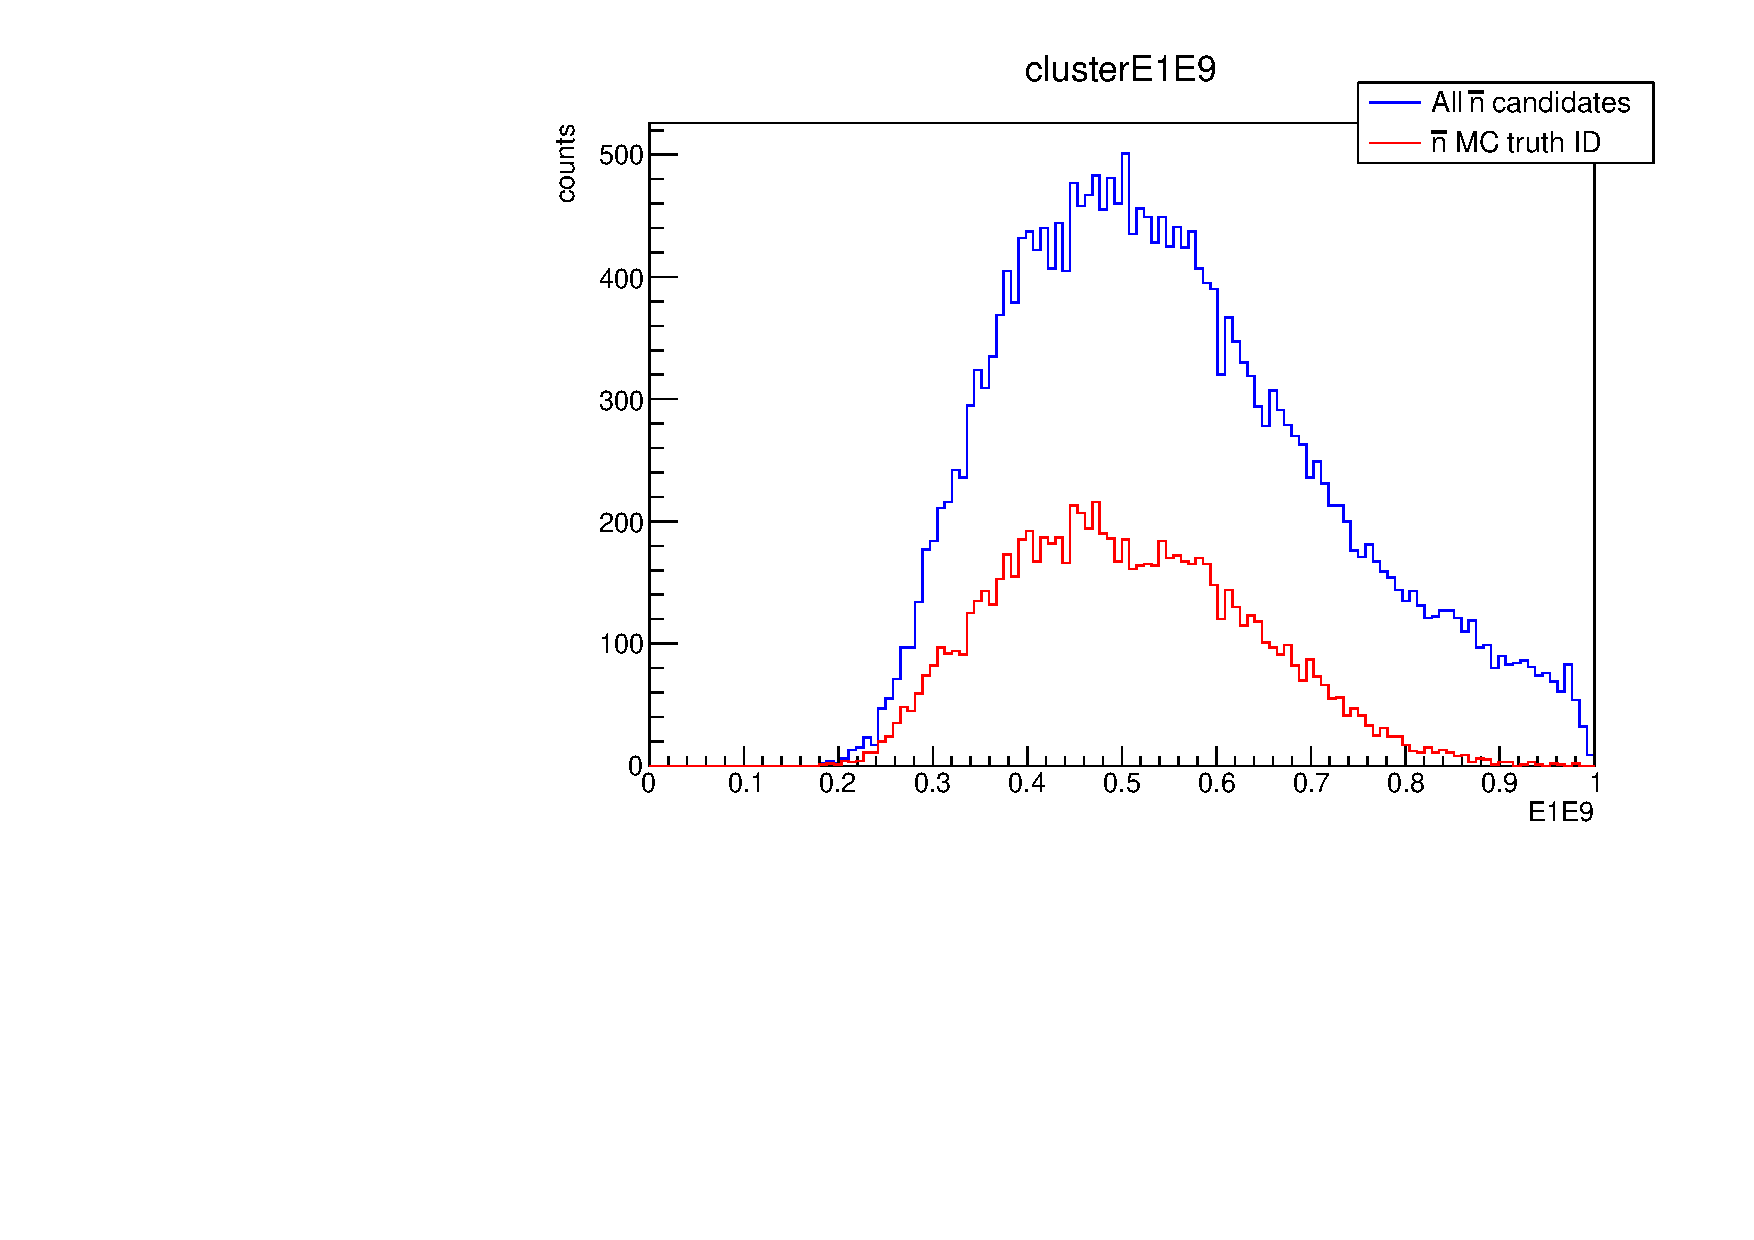
\includegraphics[width=0.49\textwidth]{nbar_MC/images/clusterE1E9_nog.pdf}
    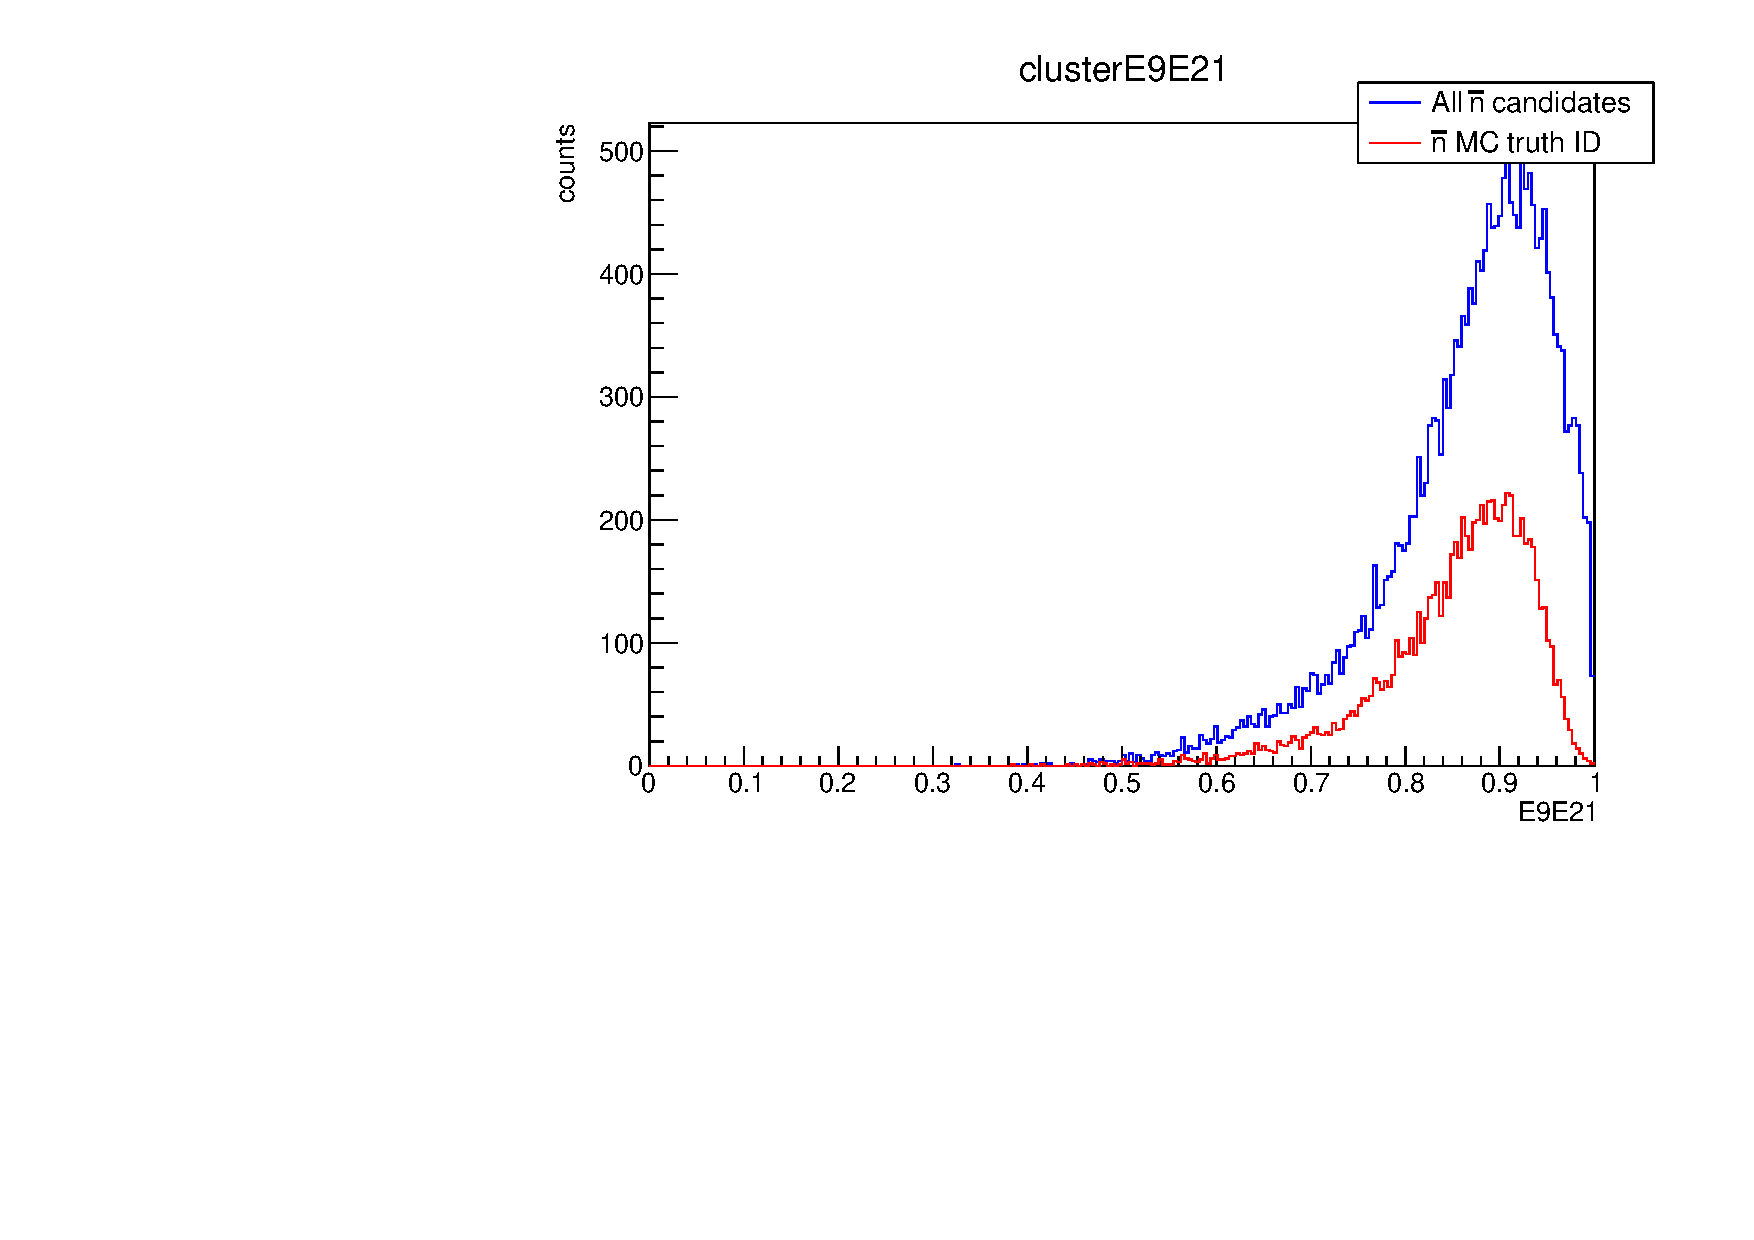
\includegraphics[width=0.49\textwidth]{nbar_MC/images/clusterE9E21_nog.pdf}
    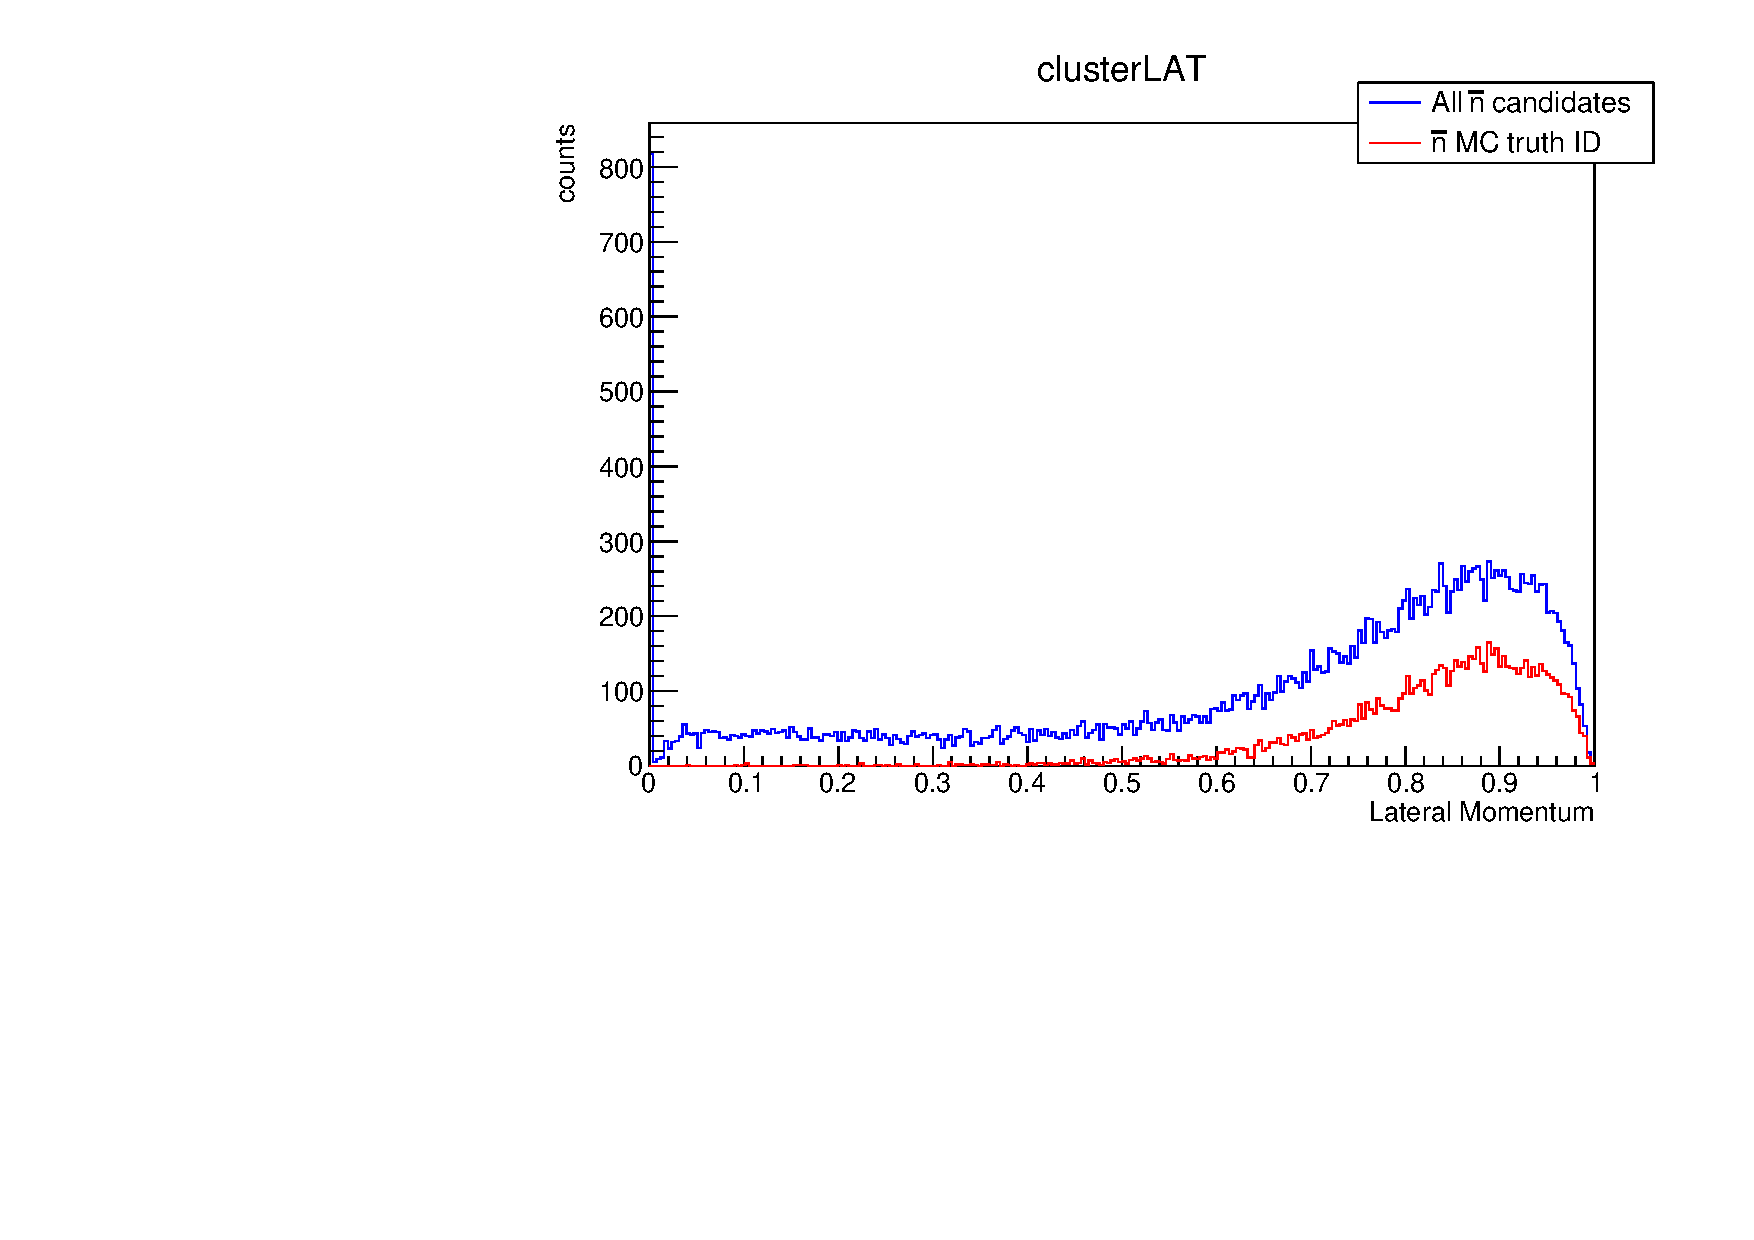
\includegraphics[width=0.49\textwidth]{nbar_MC/images/clusterLAT_nog.pdf}
    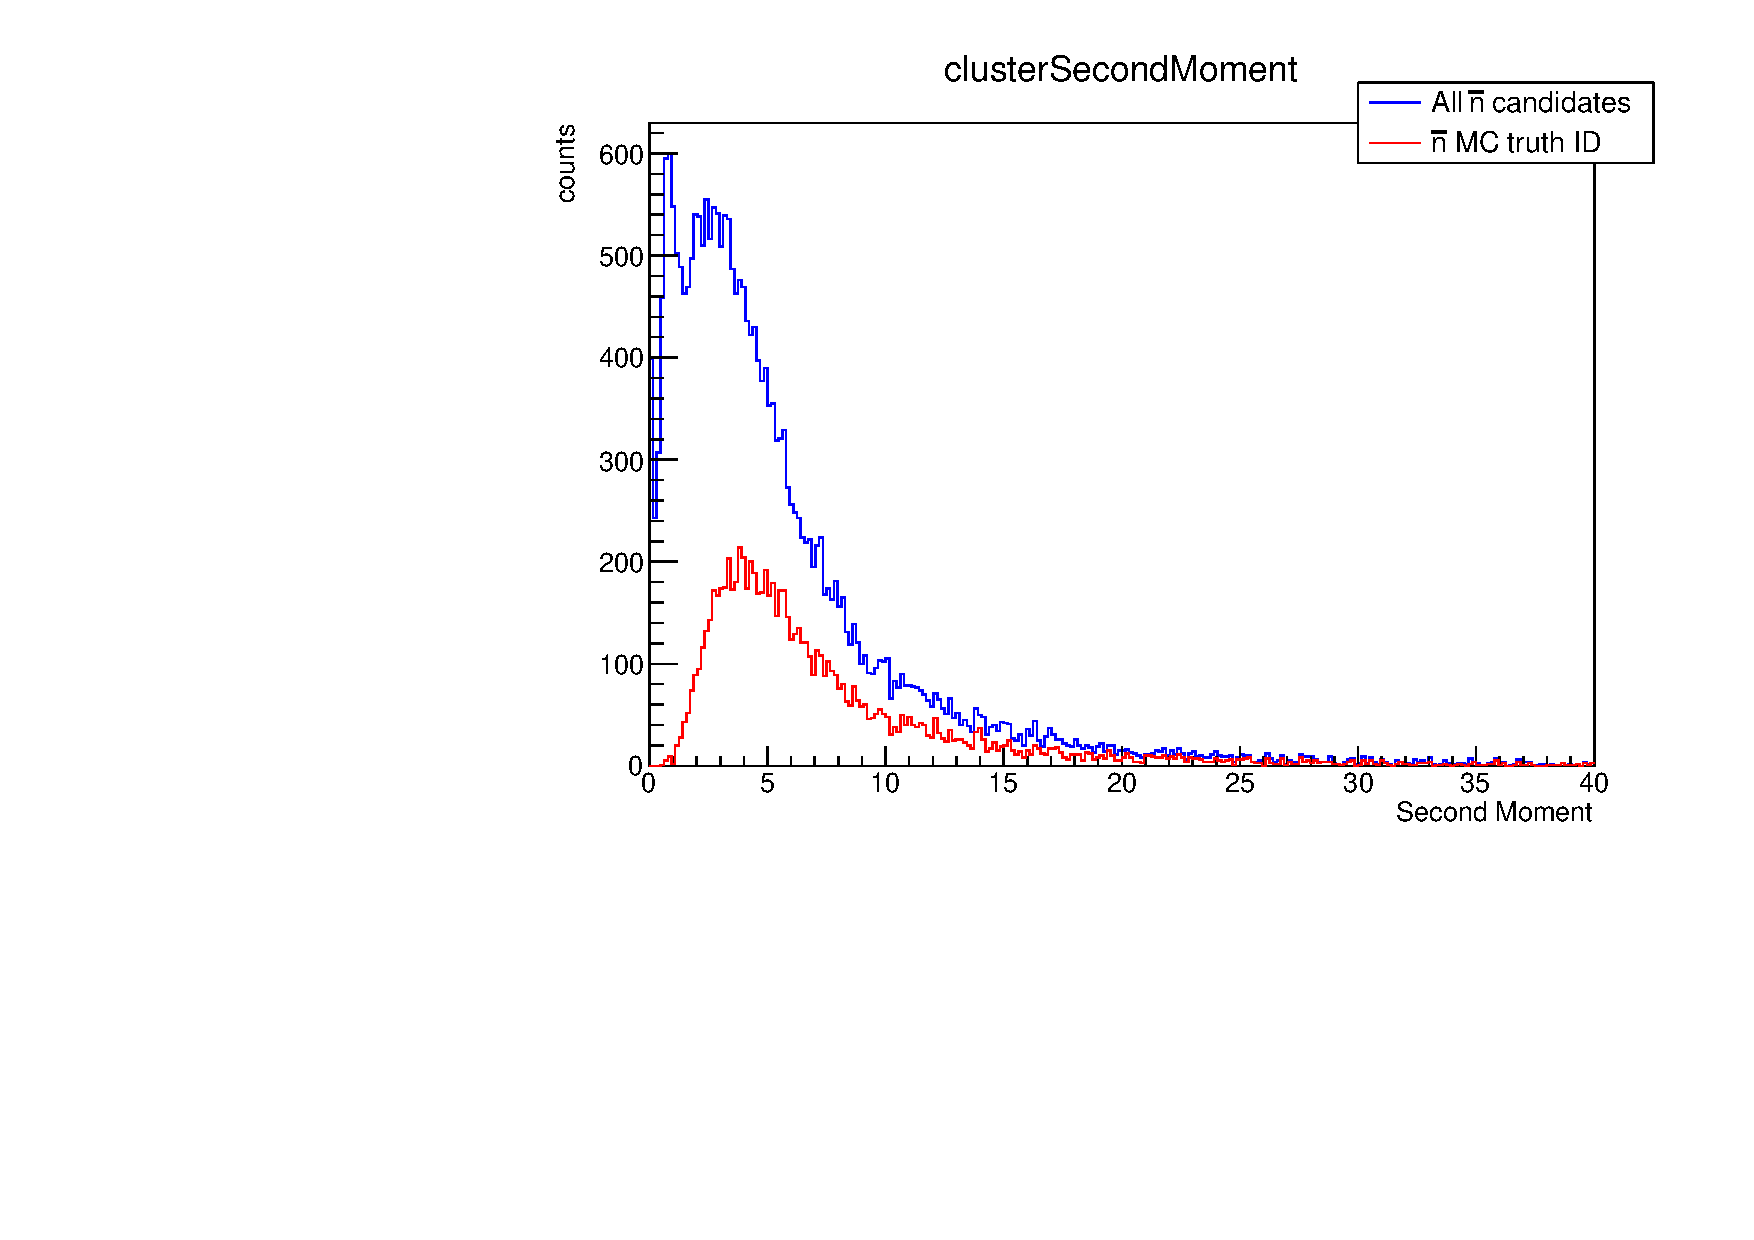
\includegraphics[width=0.49\textwidth]{nbar_MC/images/clusterSecondMoment_nog.pdf}
    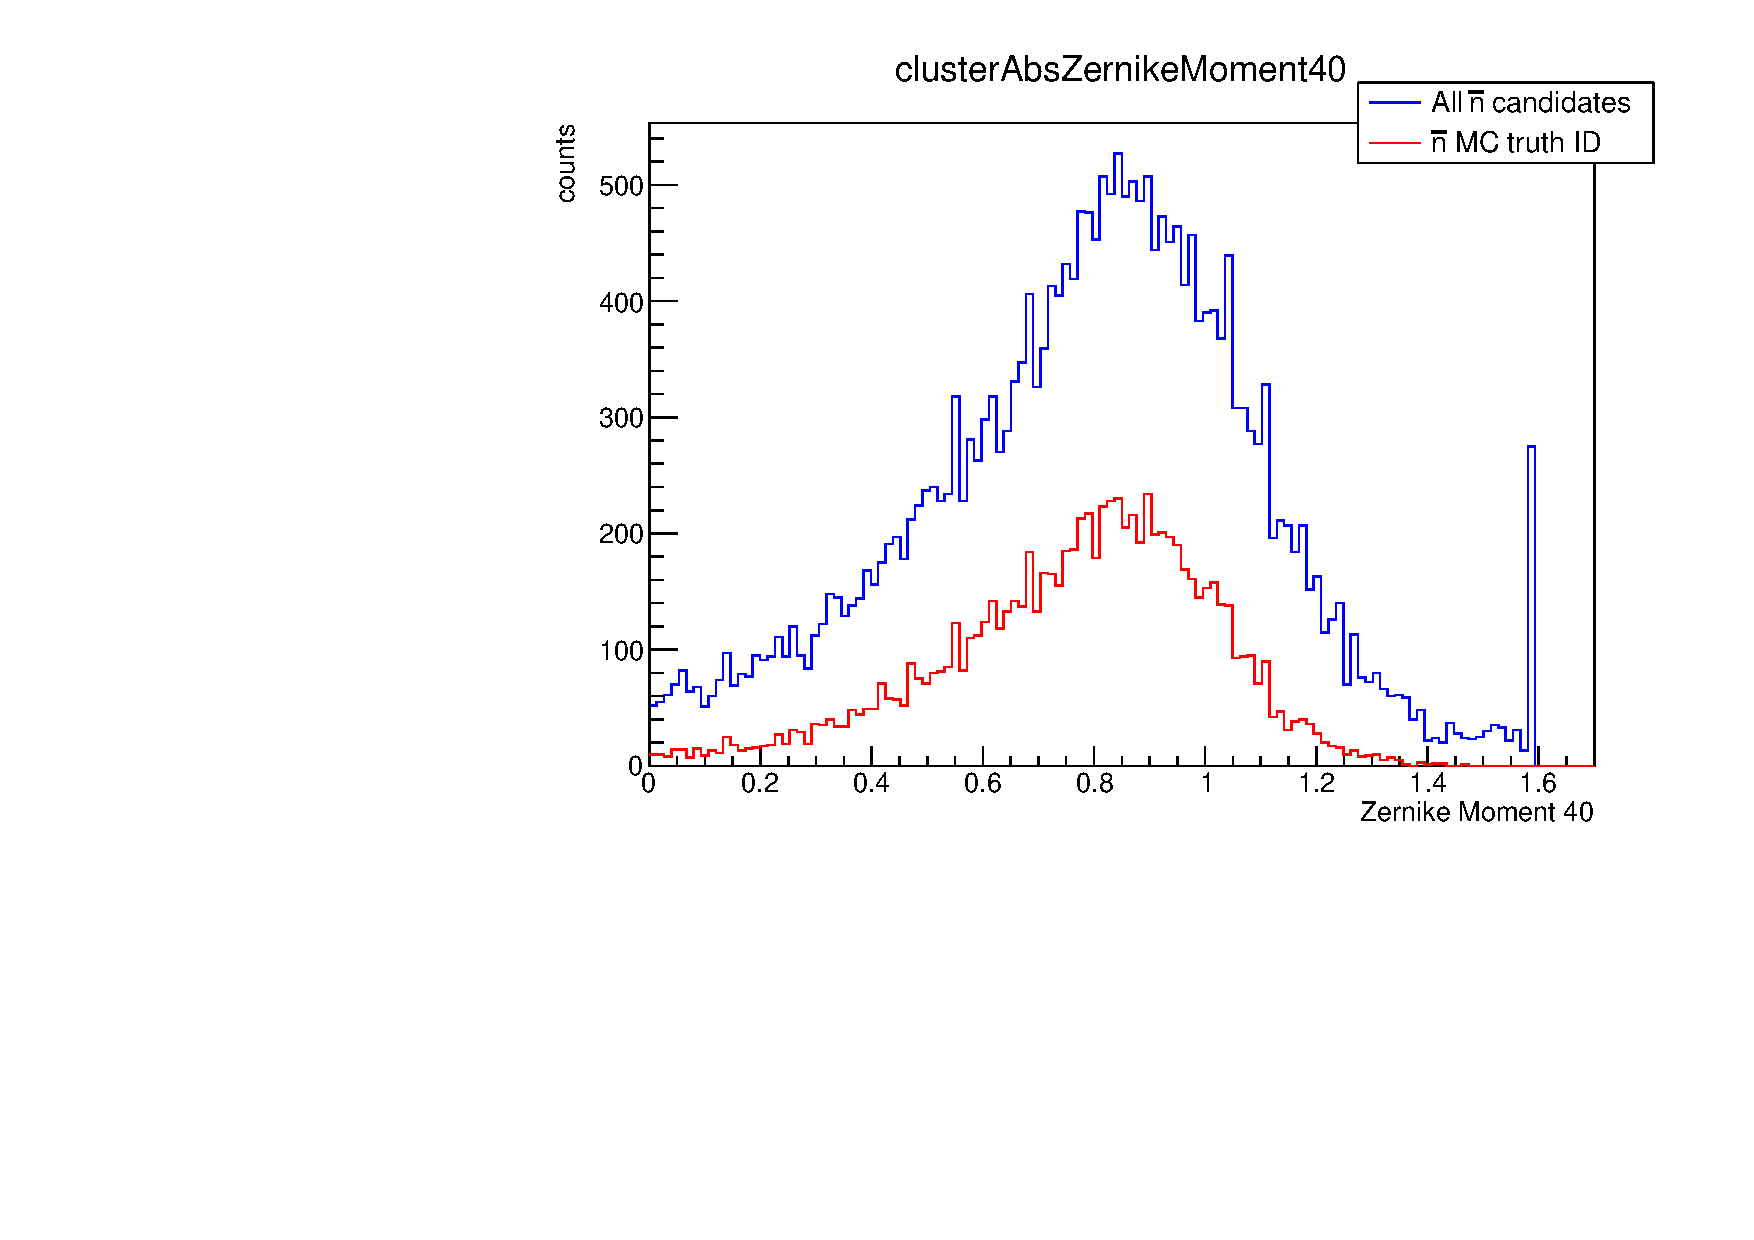
\includegraphics[width=0.49\textwidth]{nbar_MC/images/clusterAbsZernikeMoment40_nog.pdf}
    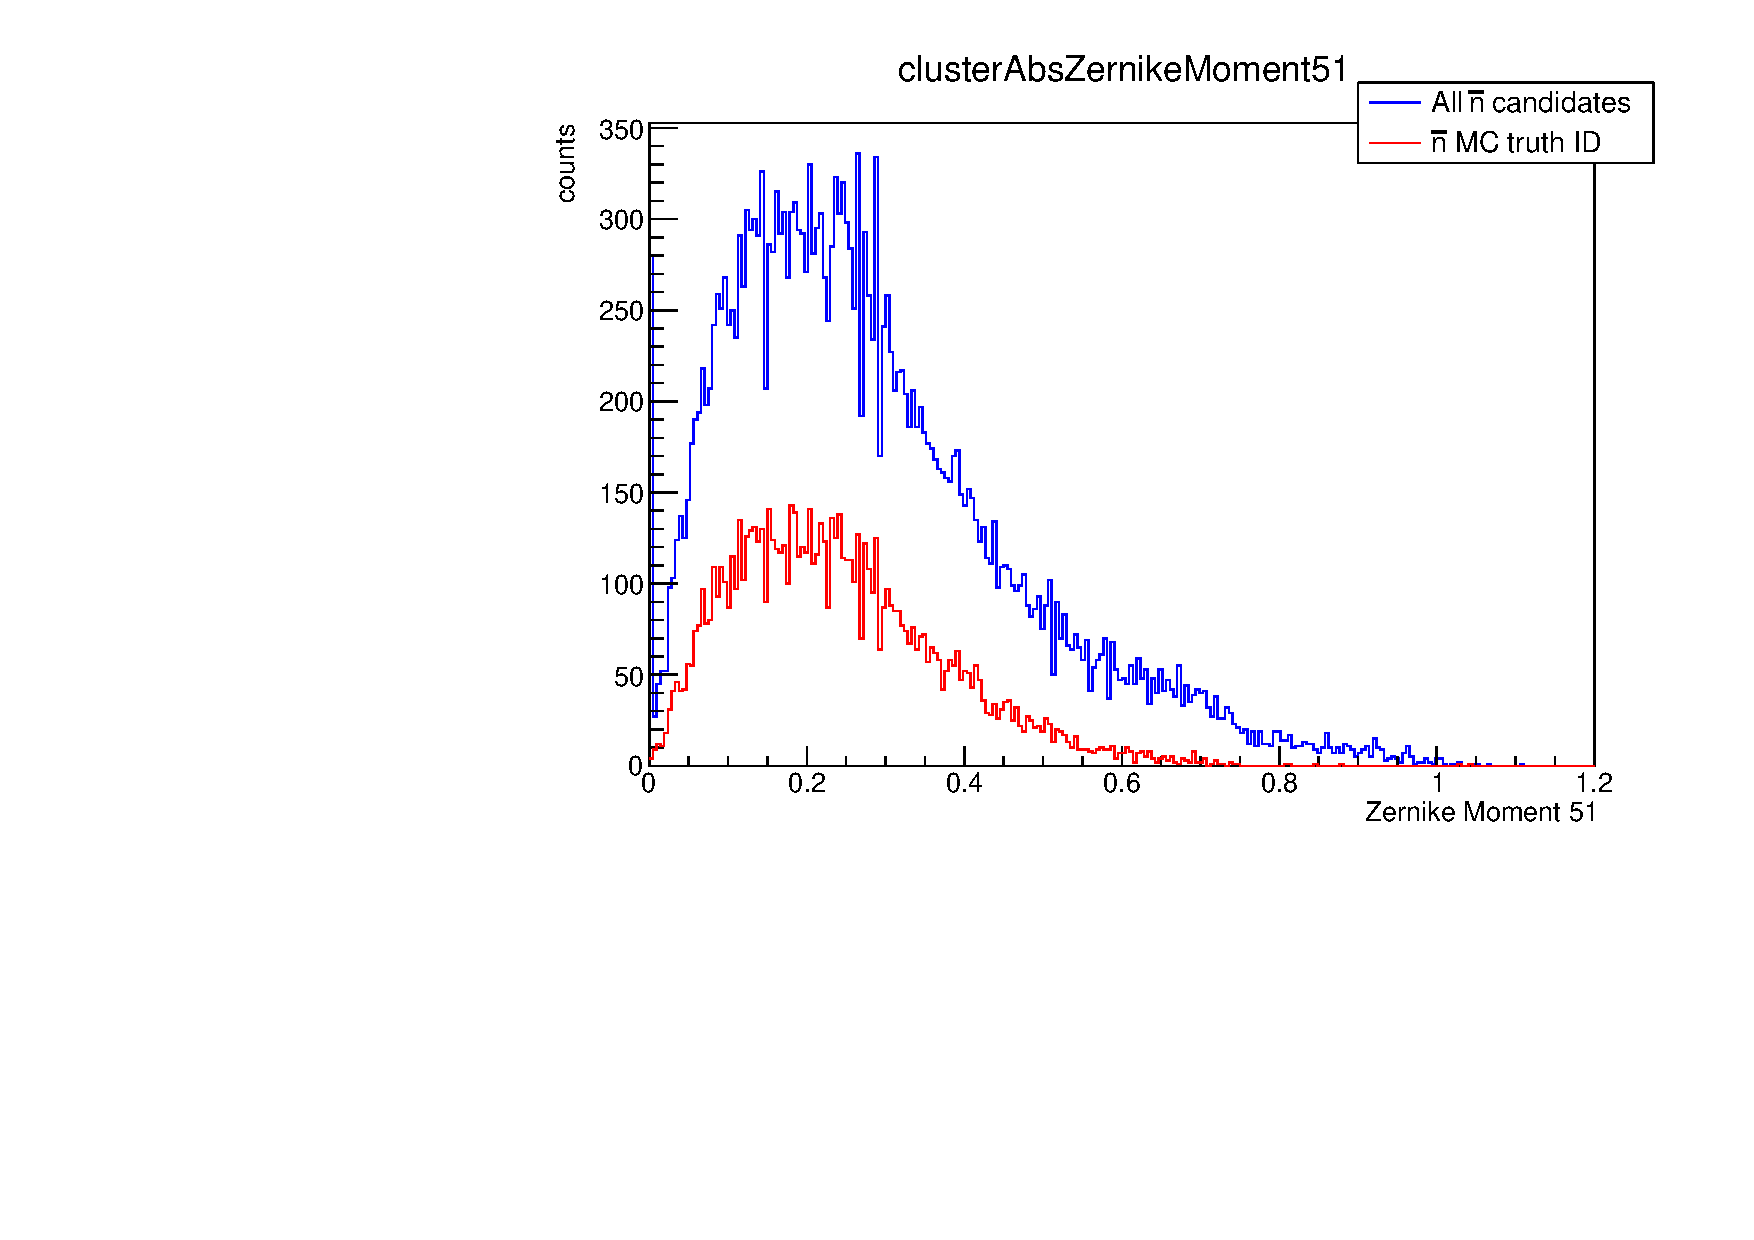
\includegraphics[width=0.49\textwidth]{nbar_MC/images/clusterAbsZernikeMoment51_nog.pdf}
    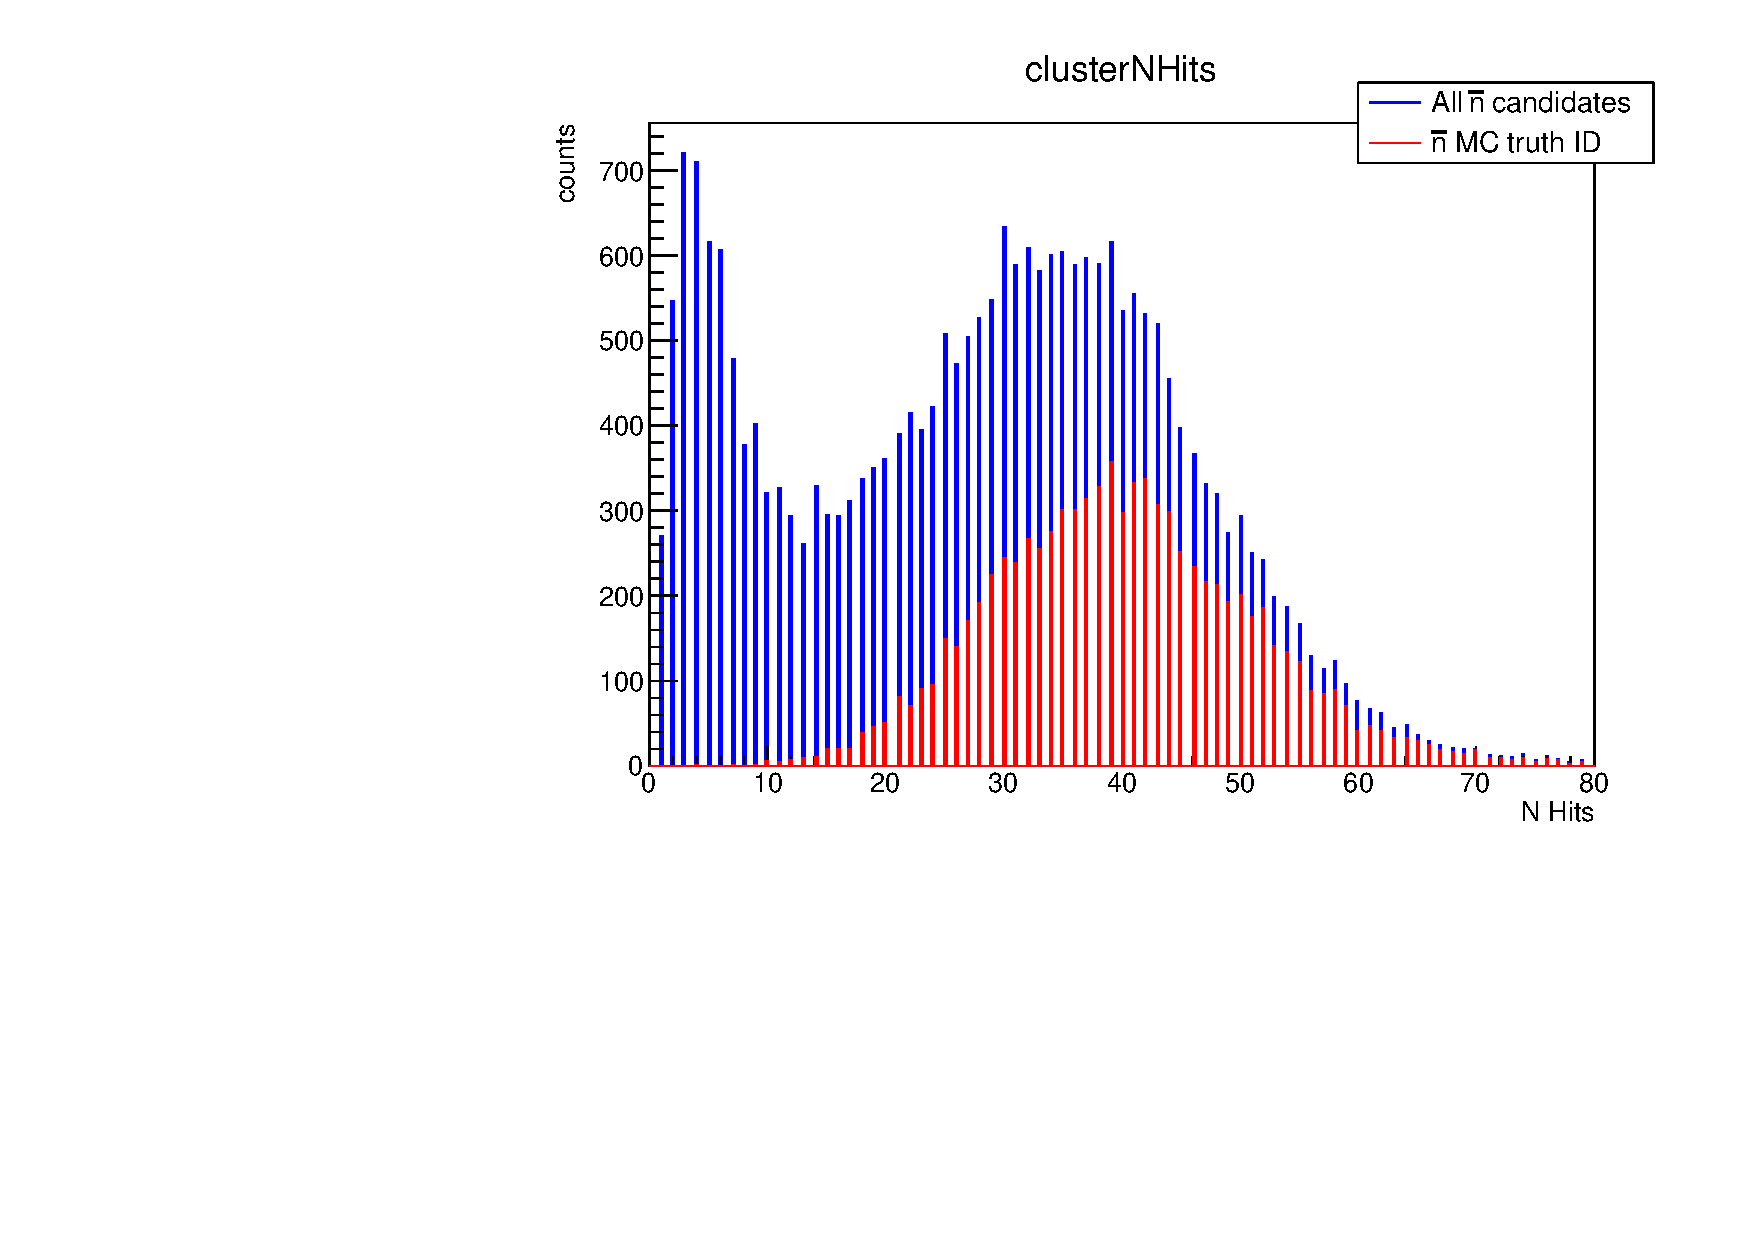
\includegraphics[width=0.49\textwidth]{nbar_MC/images/clusterNHits_nog.pdf}
   
     \caption{Comparison of reconstructed cluster variables for all $\bar{n}$ candidates versus those associated with $\bar{n}$ particles by Monte Carlo truth Monte Carlo PDG = -2112 (NO ISR case). The selection is performed using the Monte Carlo PDG code ($-2112$), as previously discussed}

\end{figure}

\newpage
First, it is important to highlight that the ISR and non-ISR distributions carry the same information, as expected. Indeed, the measurement of cluster variables is independent of the recoil system, which could be made of either $p \pi^- \gamma_{ISR}$ or $p \pi^-$ respectively.
$\\$
It is also noteworthy that the {\color{blue} blue distribution} shows some peculiar structures respect the {\color{red} red distribution}. The reconstructed cluster energy for all $\bar{n}$ candidates exhibits a first structure at low energy values that resembles those discussed for the anti-neutron momentum distributions. This is also evident in the second moment distribution, where a low-energy structure is clearly visible. The most prominent difference appears in the number of hits ($N \ Hit$) distribution, where a distinct structure at $N \ Hit < 10$ is evident.
$\\$
The nature of these characteristic structures is analyzed in the following sub-paragraph.

\subsubsection{Ancestor cluster variables}
It would be interesting to investigate the nature of this structure using the same approach as before, namely studying the ancestor contributions. The shower shapes with the following selections are compared:
\begin{itemize}
\item $\bar{n}$ Monte Carlo PDG = -2112 (neutral clusters correctly associated with $\bar{n}$ particles)
\item $\bar{n}$ Monte Carlo PDG = NaN (neutral clusters not associated with any particles)
\item $\bar{n}$ hasAncestor = 0 (neutral clusters with no $\bar{n}$ as relative)
\item $\bar{n}$ hasAncestor != 0 (neutral clusters with $\bar{n}$ as relative)
\end{itemize}

Referring to figures ~\ref{fig:cluster_ISR} and ~\ref{fig:cluster_NOISR}, as expected the neutral clusters correctly associated with $\bar{n}$ particles carry the same information of those without $\bar{n}$ as relative, in bot ISR and NO ISR cases.
$\\$
Furthermore, it is evident how reconstructed neutral clusters not associated with any particles by the Monte Carlo and those with $\bar{n}$ as relative are primarily responsible for the structures observed at low values of energy, second moment, and number of crystals.
$\\$
A further selection on number of crystals ($clusterNHits > 10$) can be performed to study the corresponding cluster variables. The result is shown in figure  ~\ref{fig:cluster_ISR_NHits} and ~\ref{fig:cluster_NOISR_NHits}. 
$\\$
As observed, these structures arise from small-sized clusters produced by $\bar{n}$ particles that undergo phenomena -such as cluster split-off and pre-showering- prior to neutral cluster formation for $\bar{n}$ candidates, as confirmed by ancestor studies. The requirement of at least 10 crystals eliminates these structures.
\newpage
The obtained cluster variables in  ISR case are shown below:
 \begin{figure}[H]
    \centering
    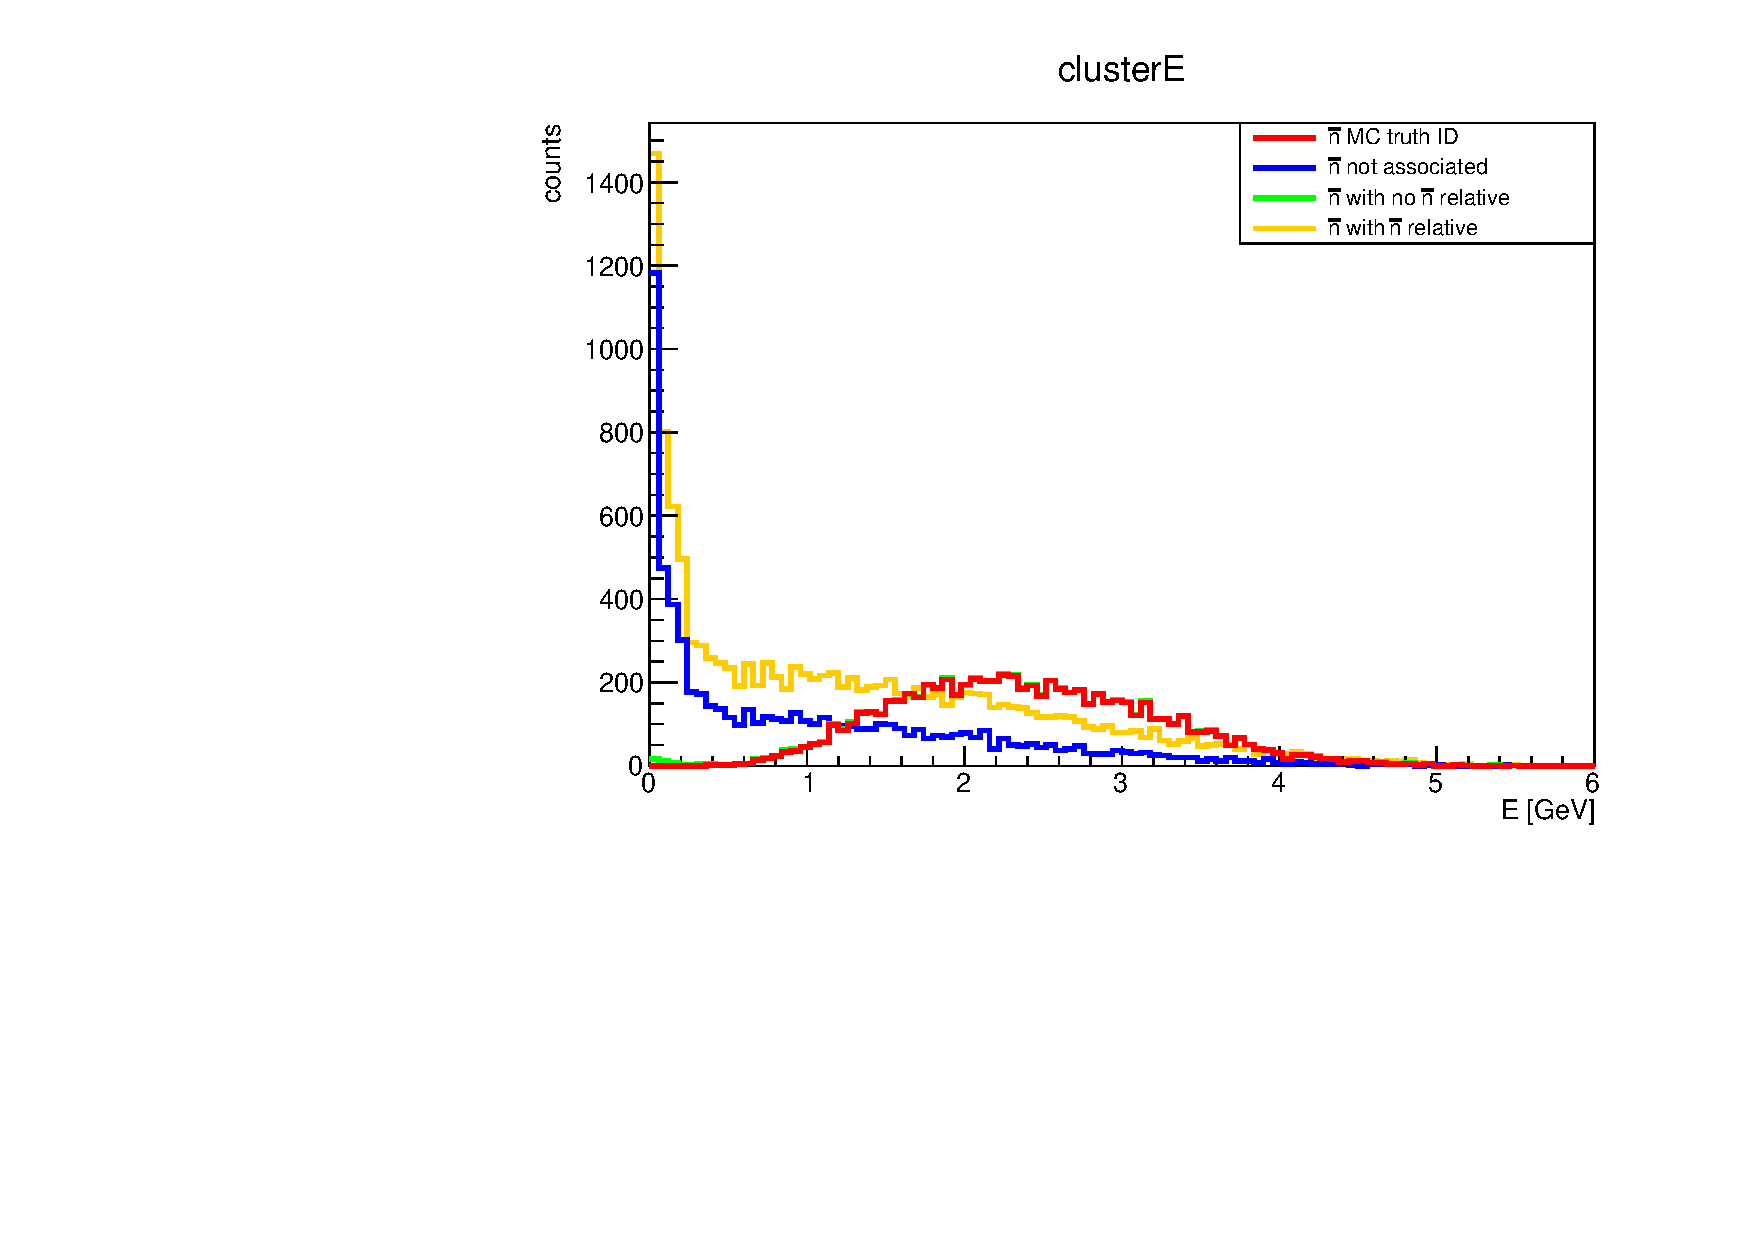
\includegraphics[width=0.49\textwidth]{nbar_MC/images/clusterE_isr_ancestor.pdf}
    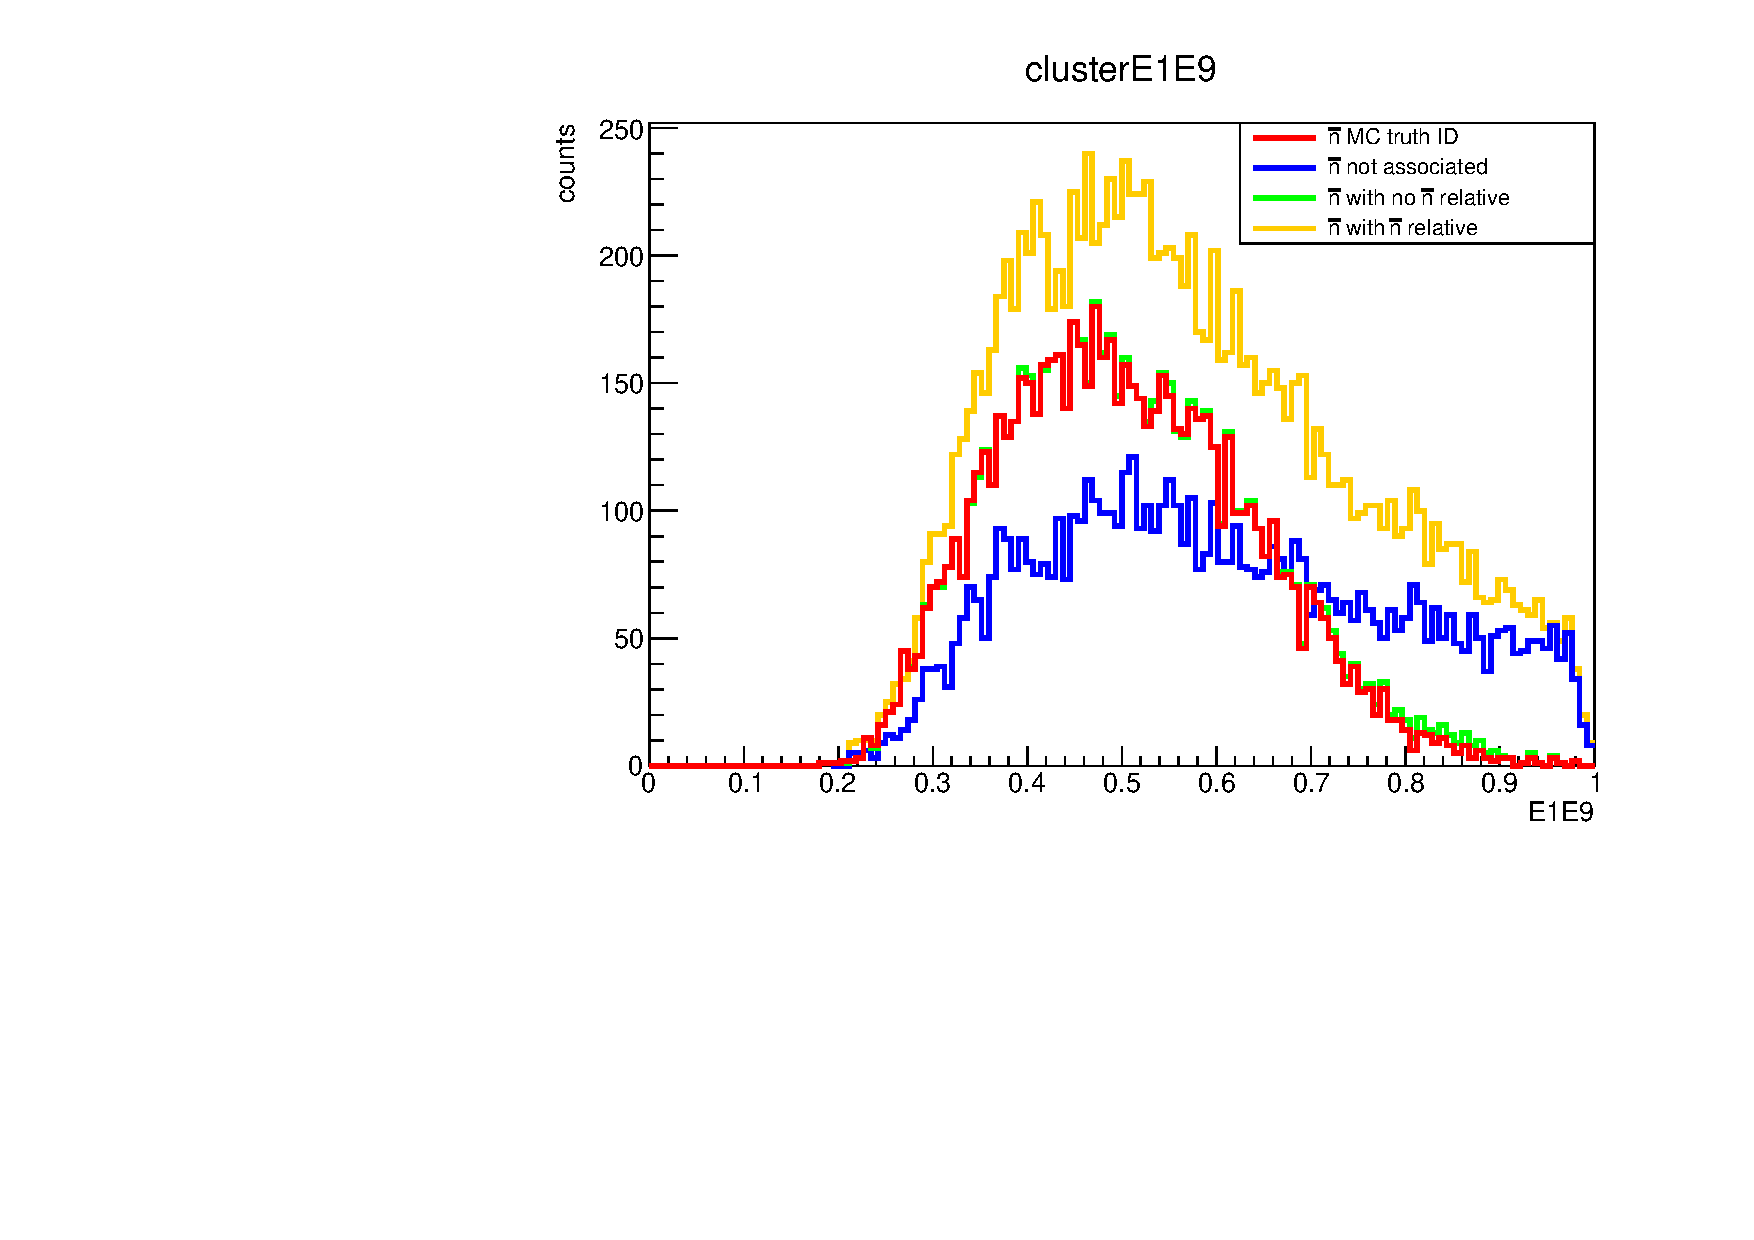
\includegraphics[width=0.49\textwidth]{nbar_MC/images/clusterE1E9_isr_ancestor.pdf}
    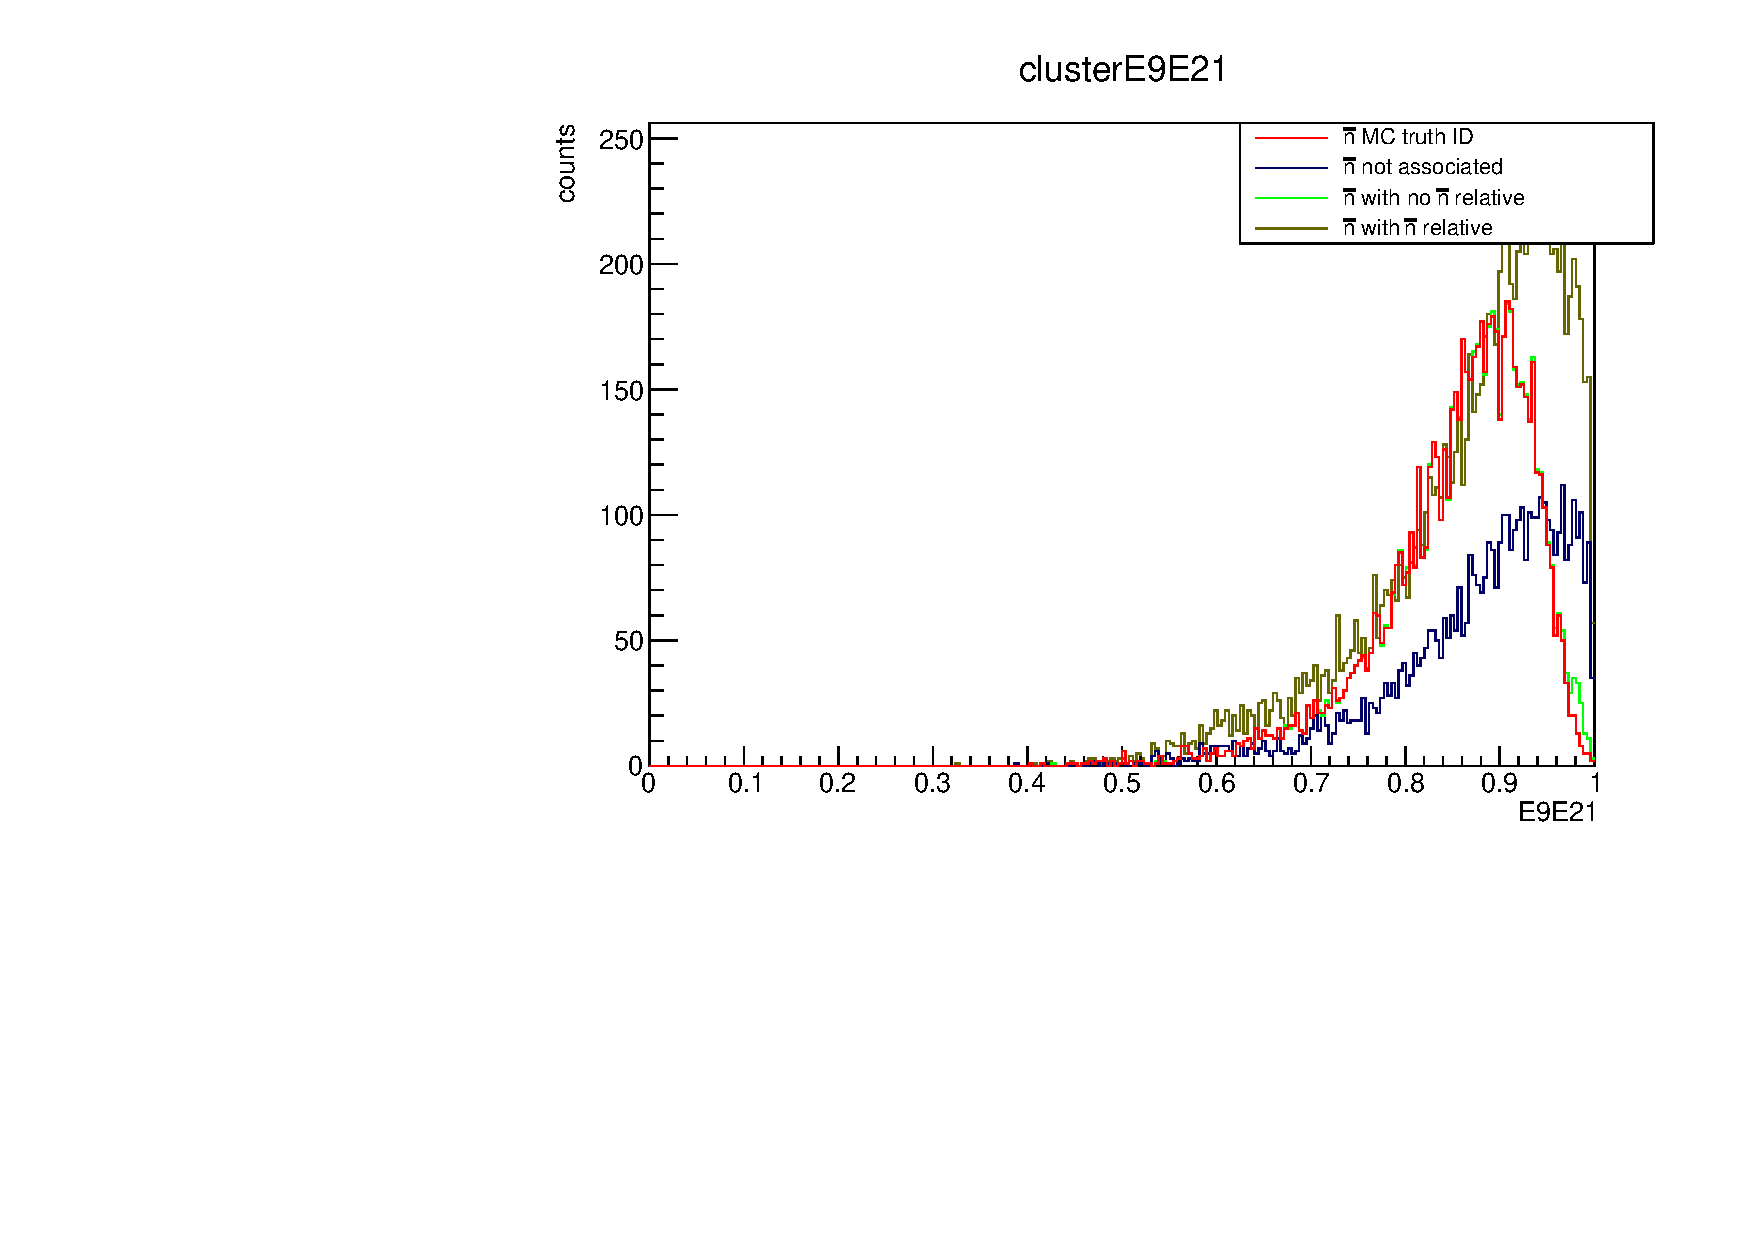
\includegraphics[width=0.49\textwidth]{nbar_MC/images/clusterE9E21_isr_ancestor.pdf}
    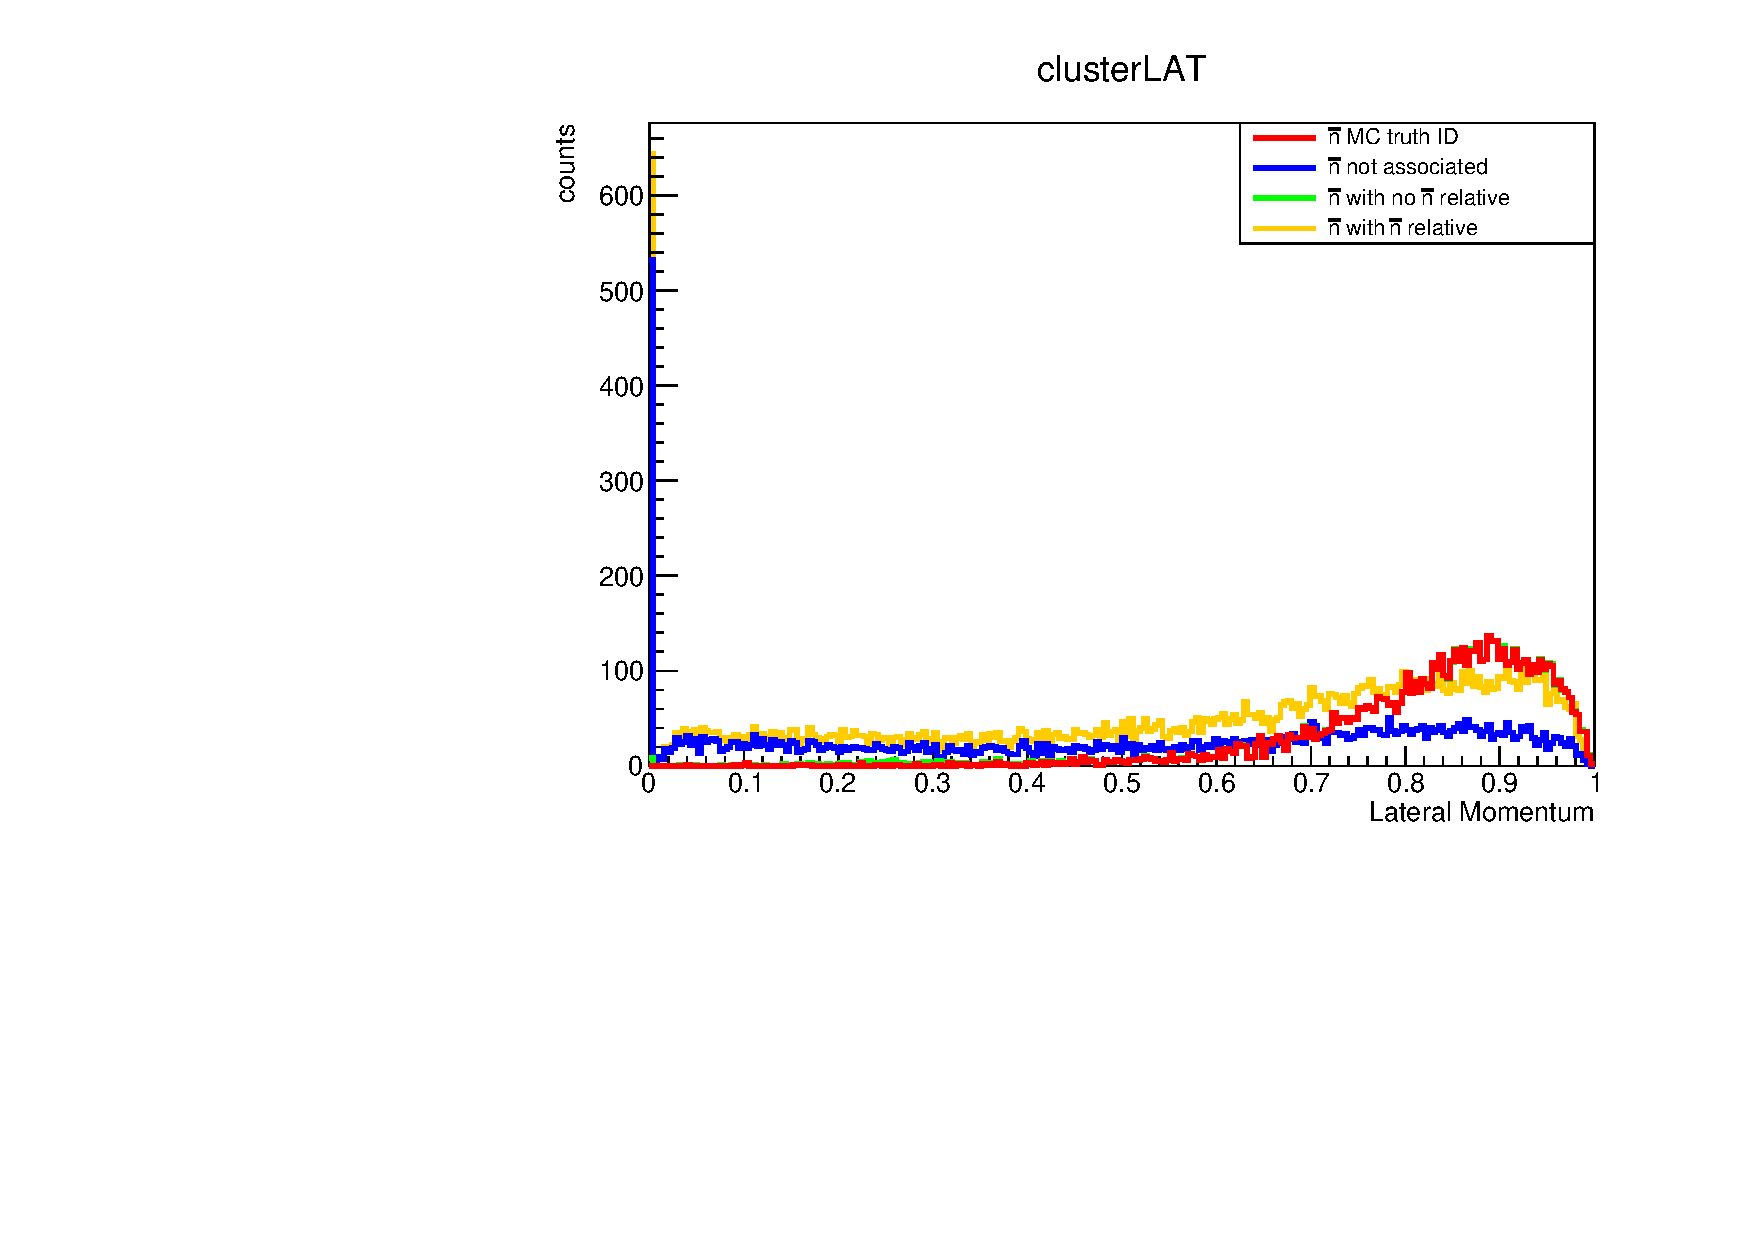
\includegraphics[width=0.49\textwidth]{nbar_MC/images/clusterLAT_isr_ancestor.pdf}
    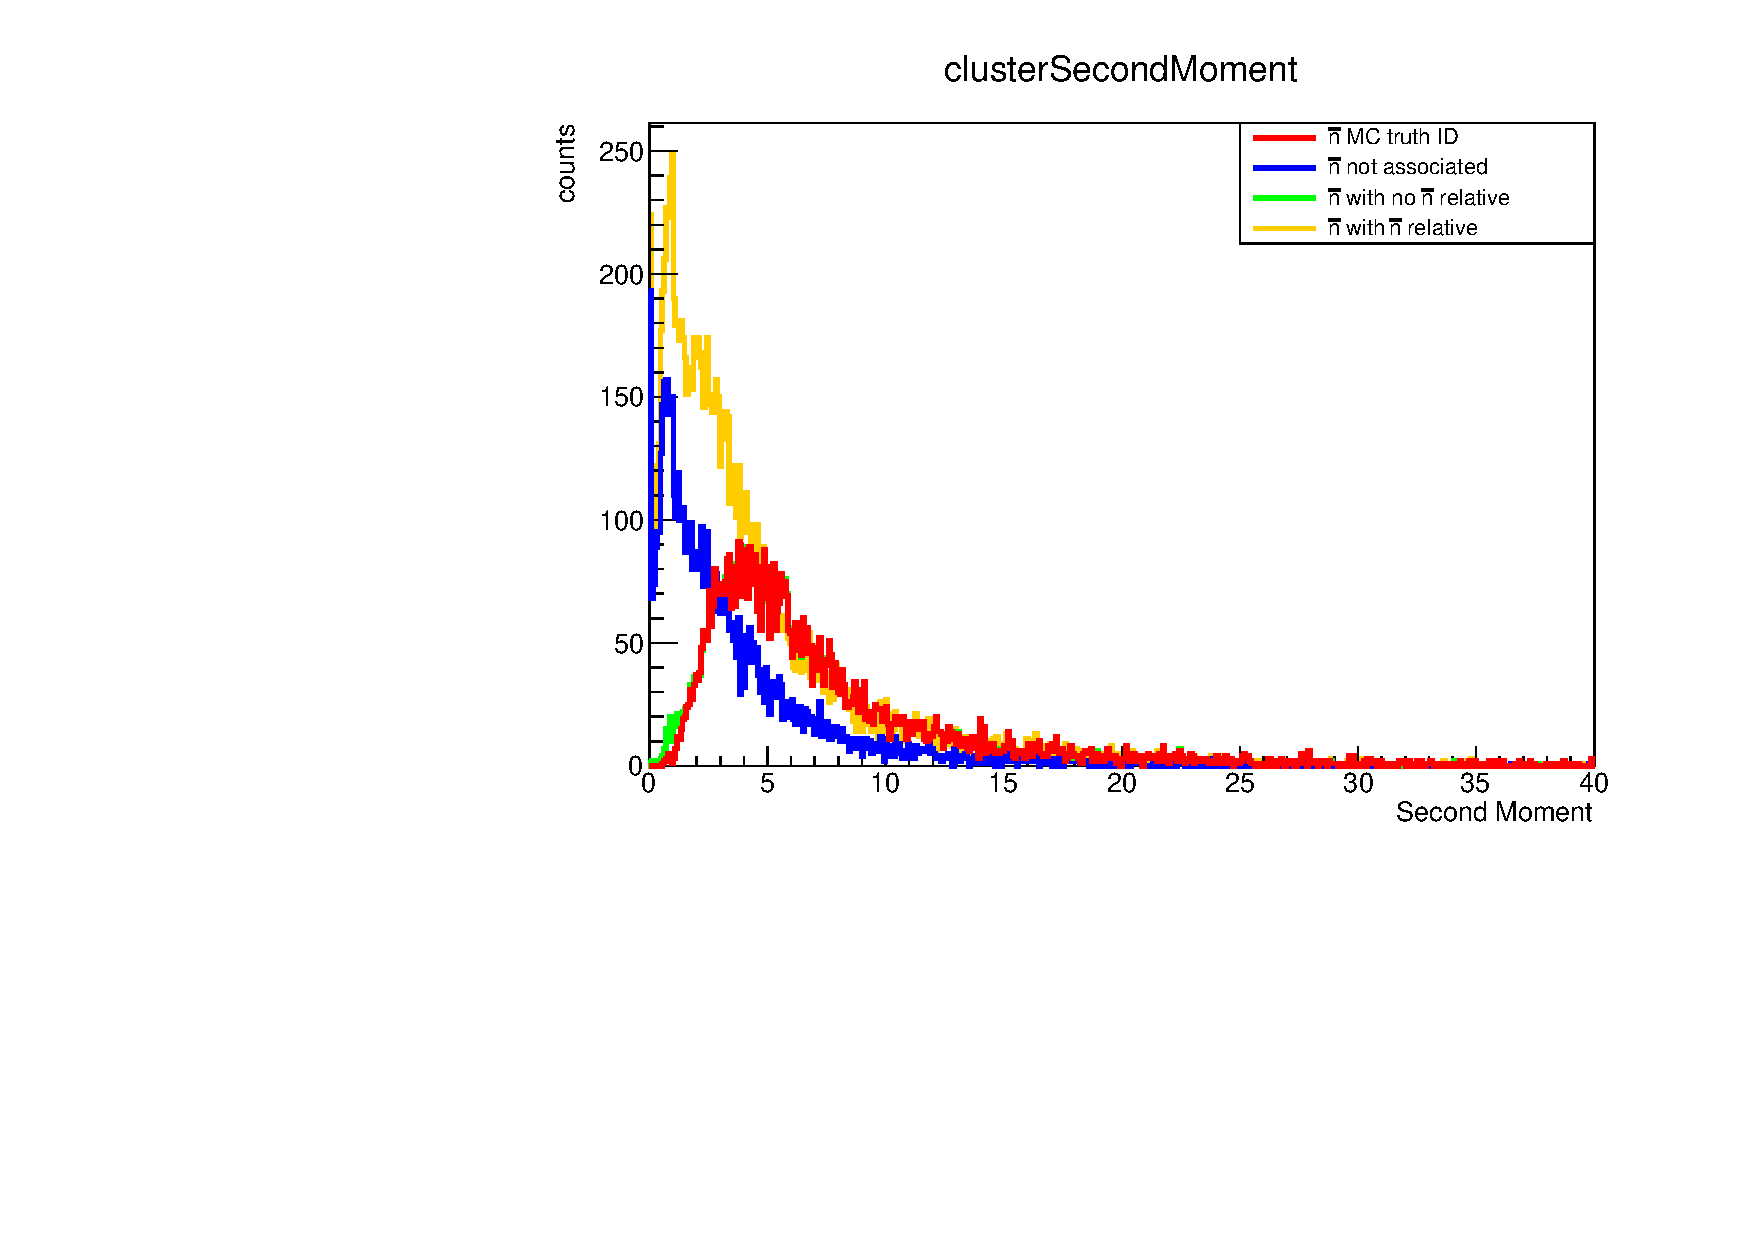
\includegraphics[width=0.49\textwidth]{nbar_MC/images/clusterSecondMoment_isr_ancestor.pdf}
    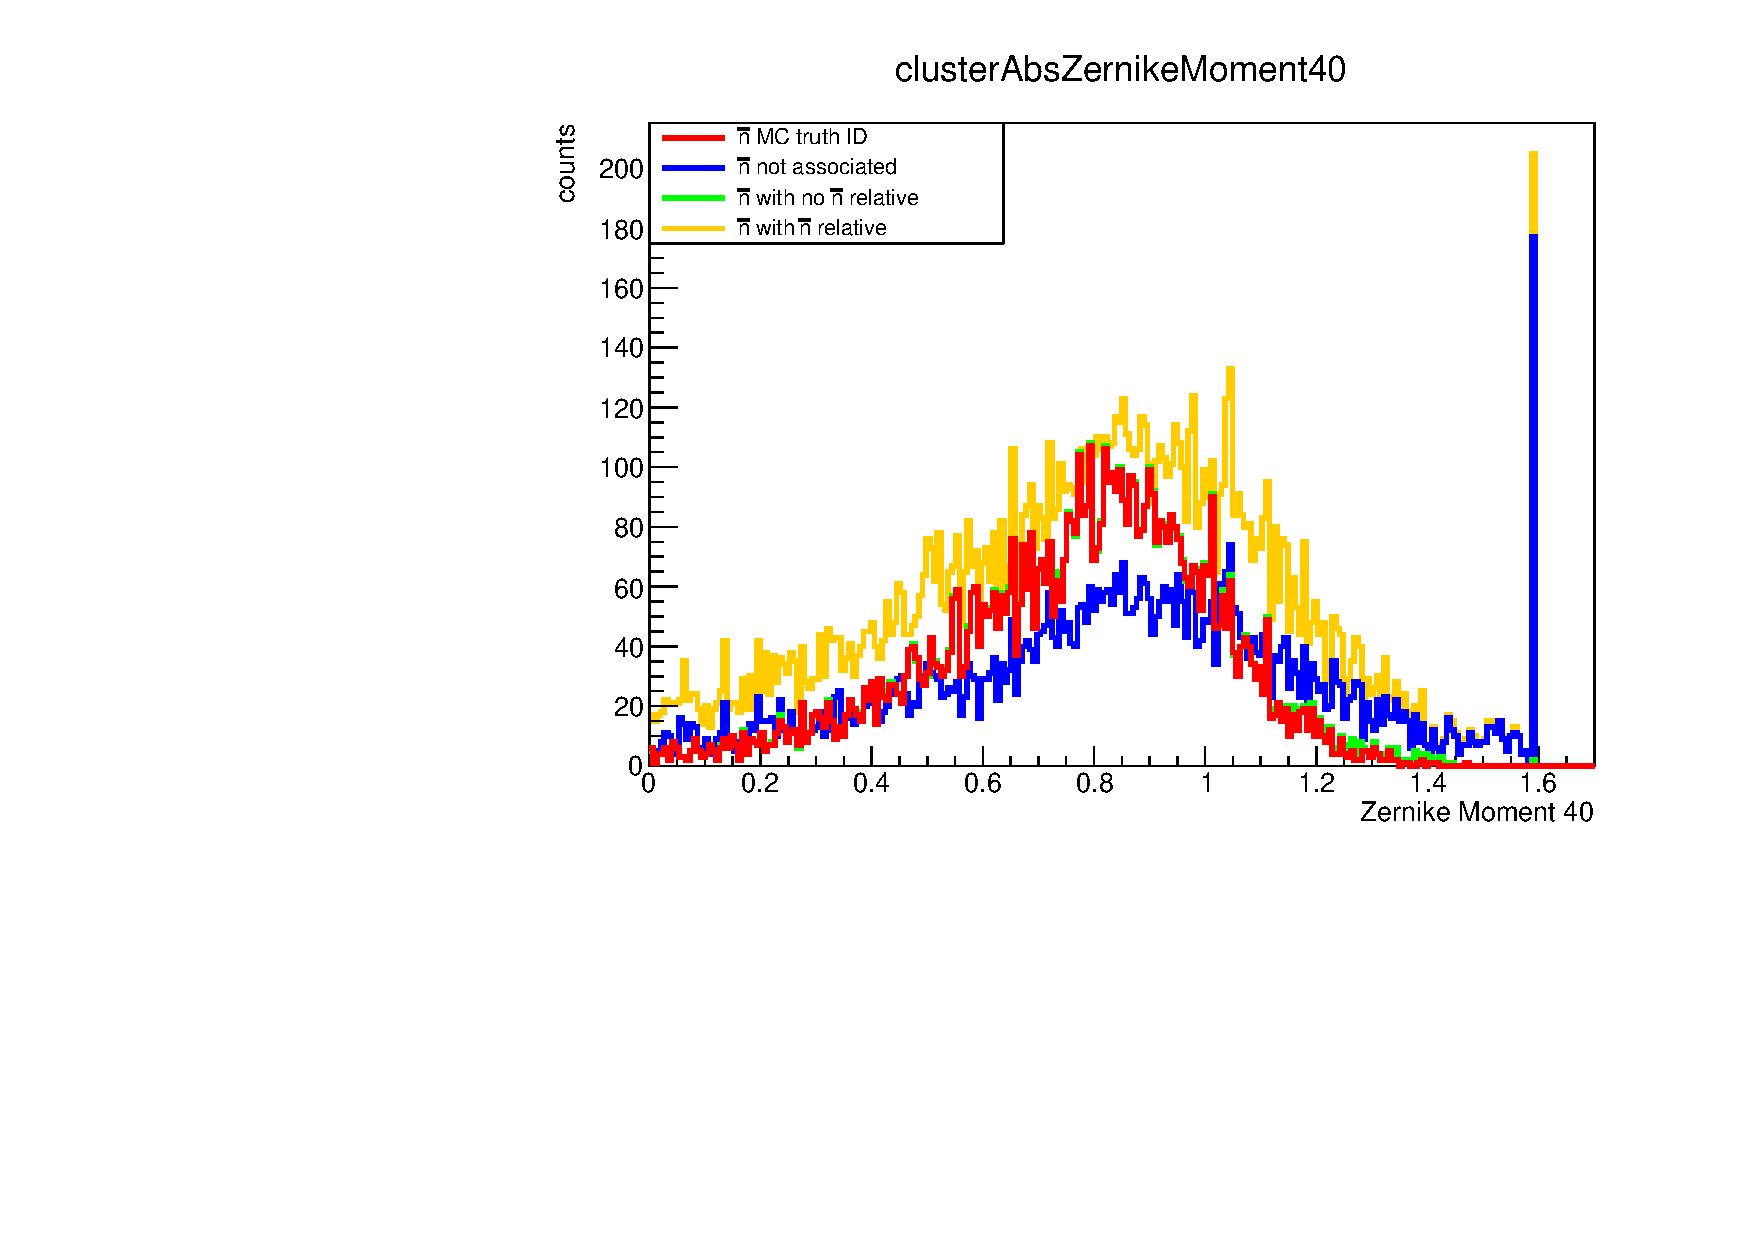
\includegraphics[width=0.49\textwidth]{nbar_MC/images/clusterAbsZernikeMoment40_isr_ancestor.pdf}
    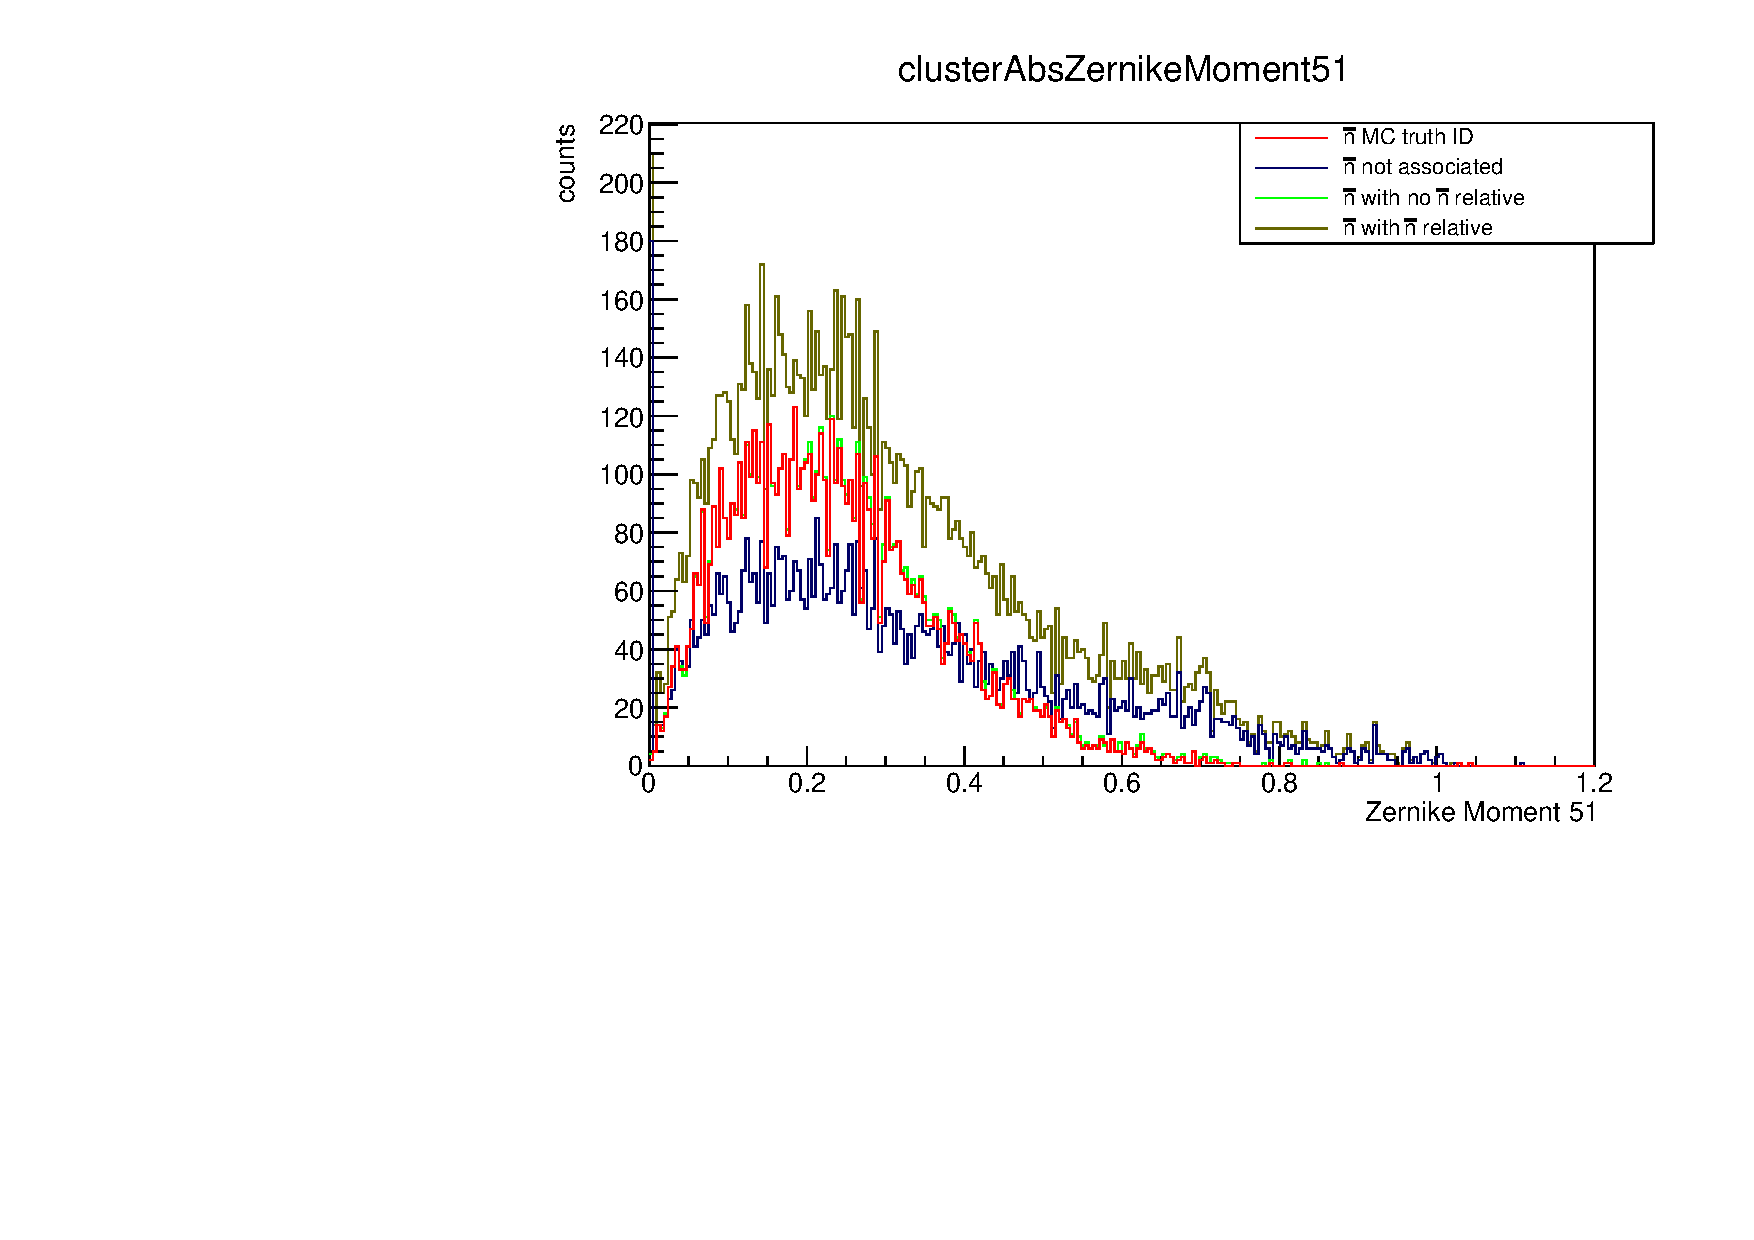
\includegraphics[width=0.49\textwidth]{nbar_MC/images/clusterAbsZernikeMoment51_isr_ancestor.pdf}
    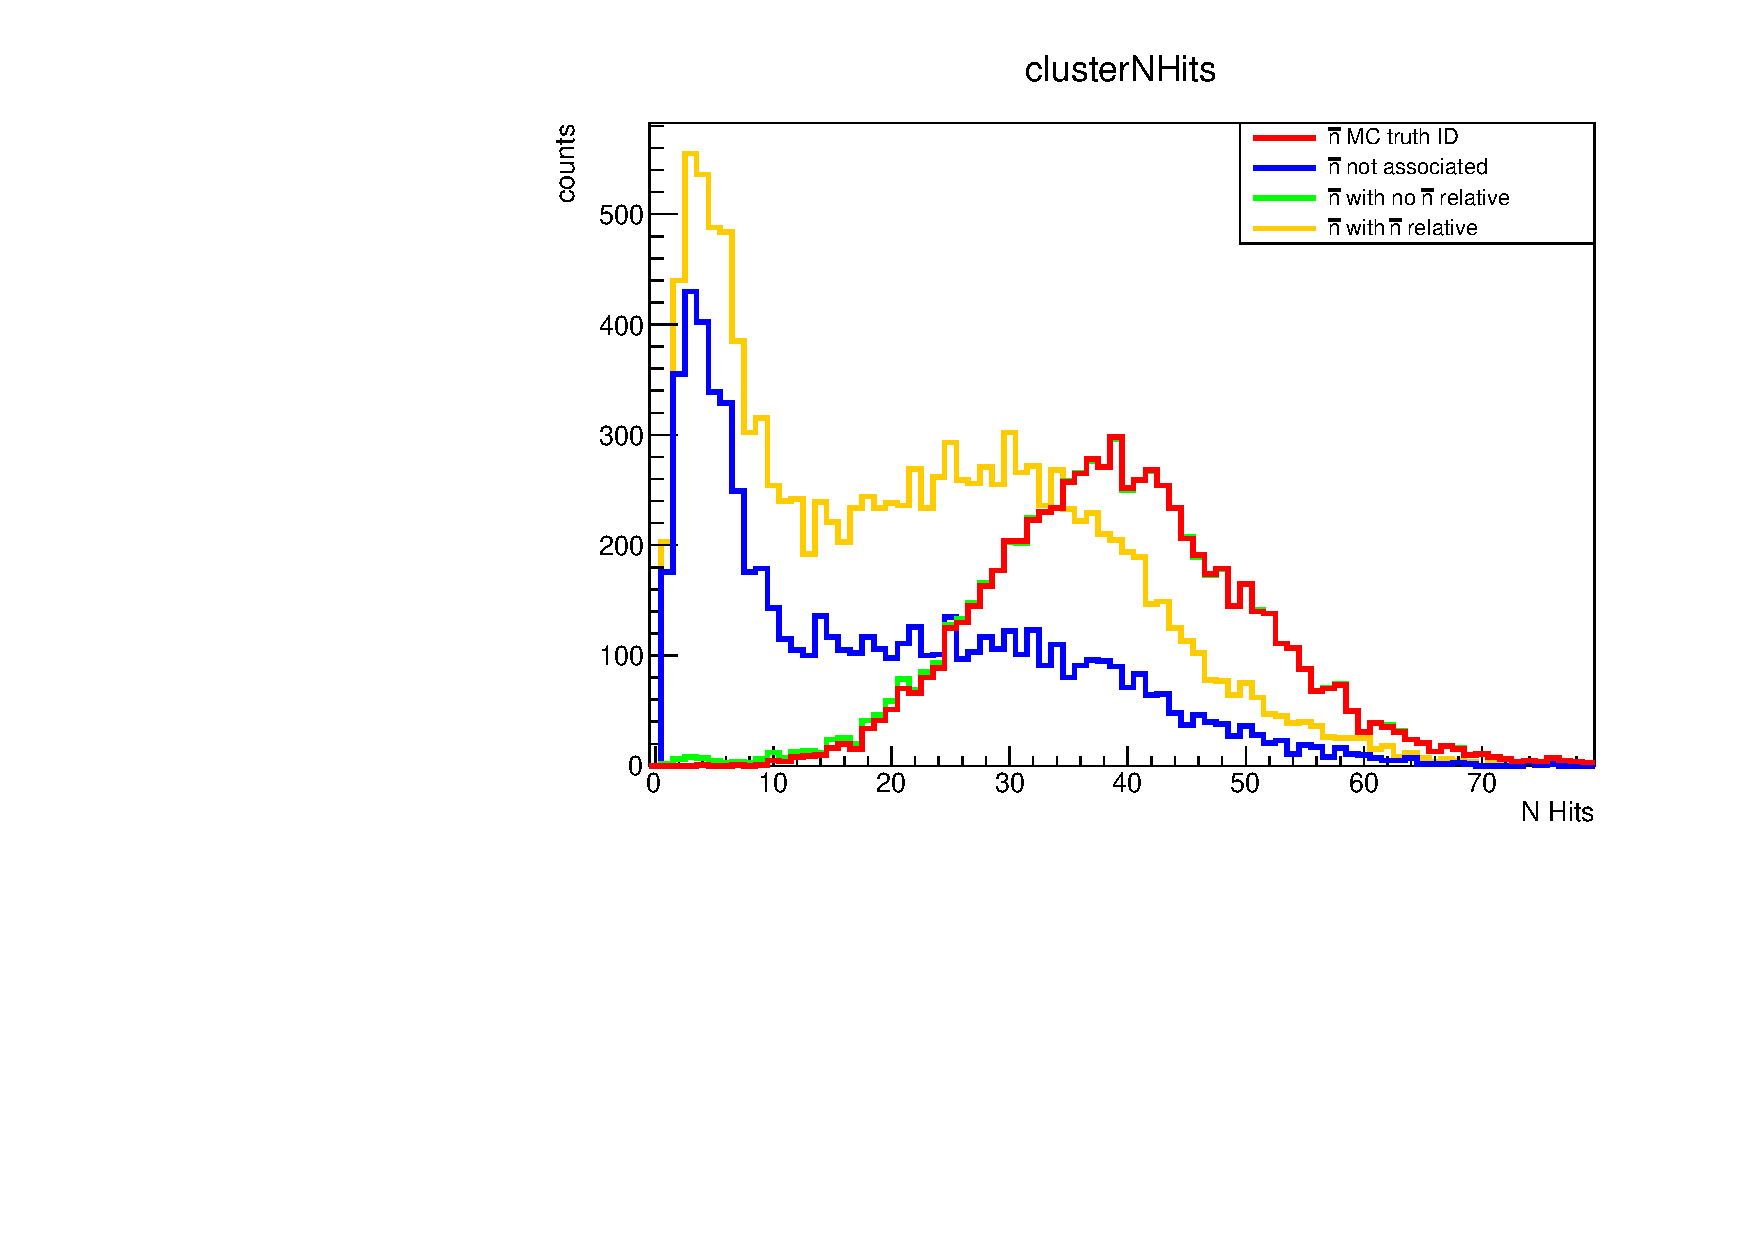
\includegraphics[width=0.49\textwidth]{nbar_MC/images/clusterNHits_isr_ancestor.pdf}
   
     \caption{Comparison of reconstructed cluster variables for $\bar{n}$ candidates with different ancestor selection (ISR case)}
     \label{fig:cluster_ISR}
\end{figure}

\newpage
The obtained cluster variables in NO ISR case are shown below:
 \begin{figure}[H]
    \centering
    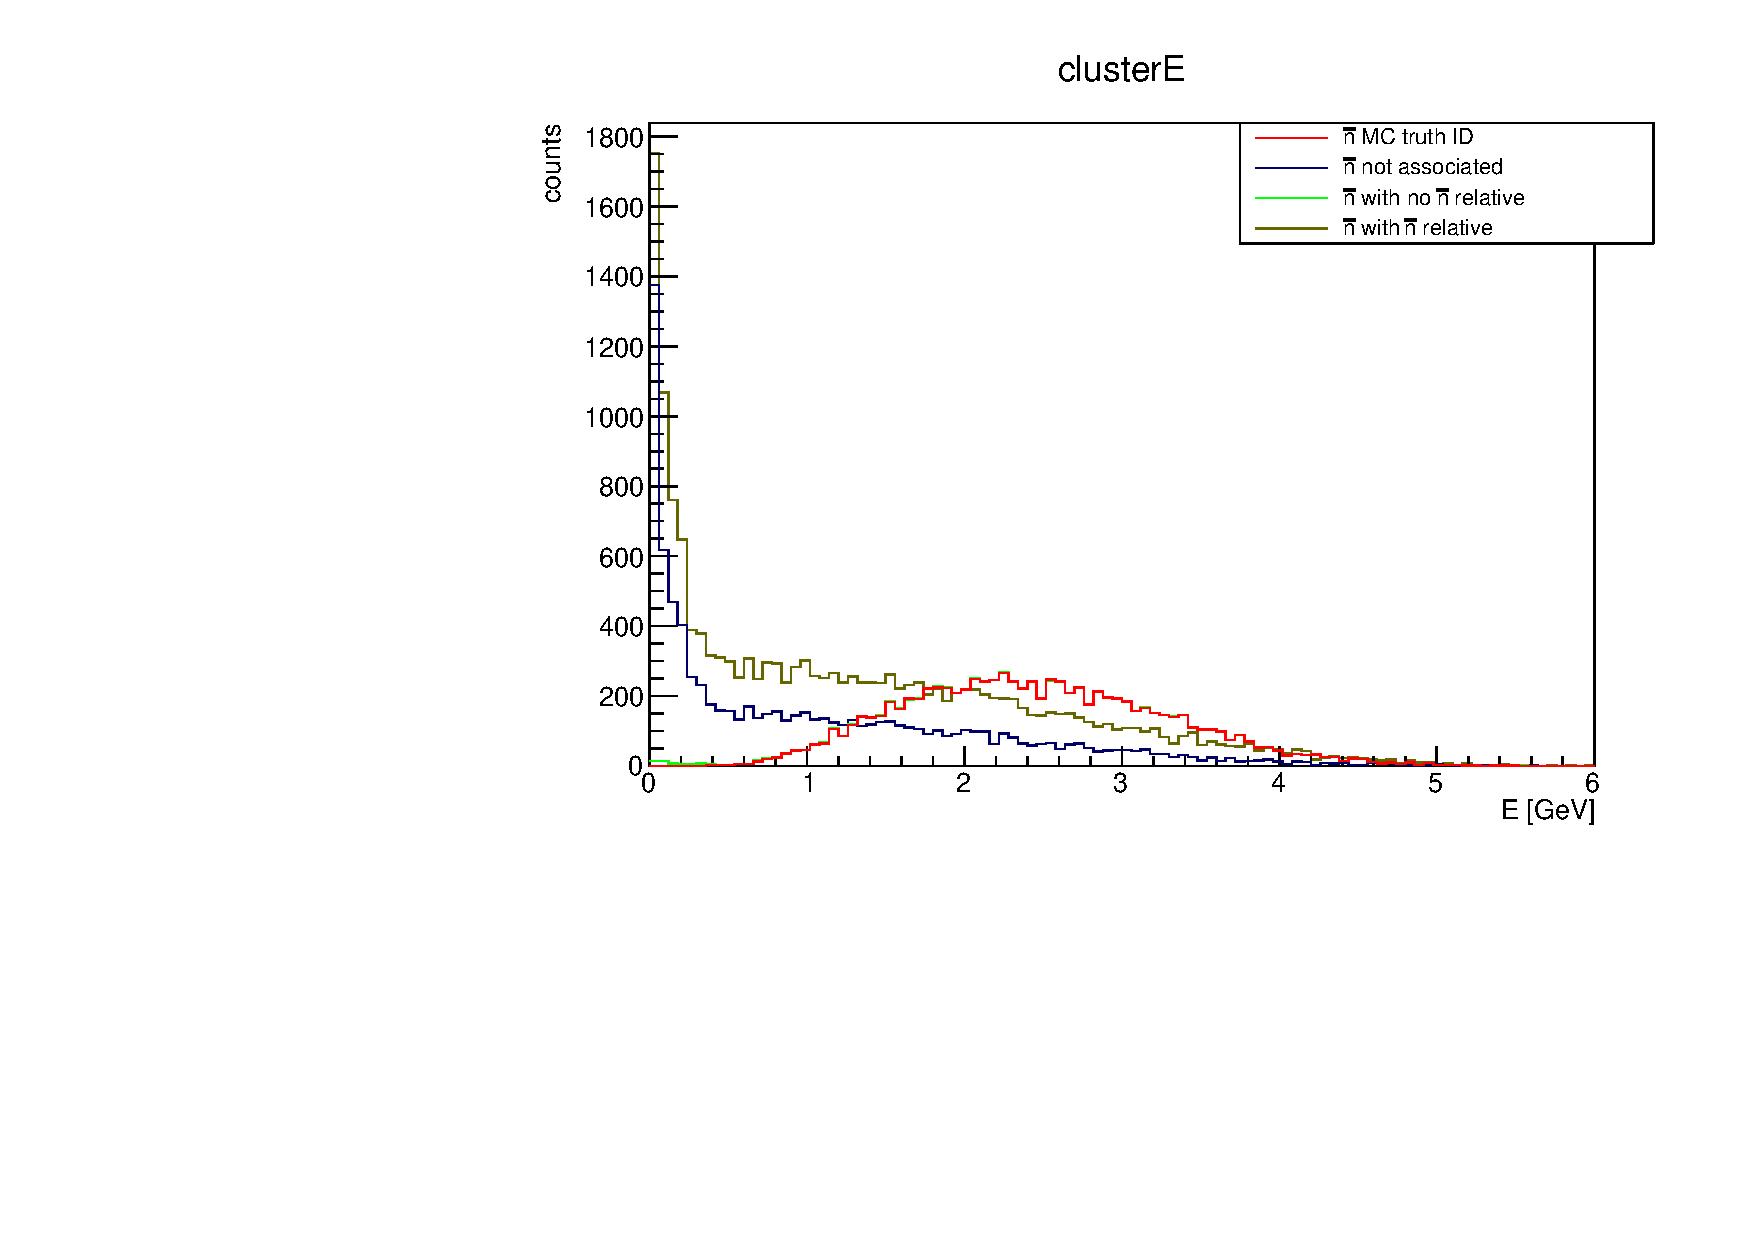
\includegraphics[width=0.49\textwidth]{nbar_MC/images/clusterE_nog_ancestor.pdf}
    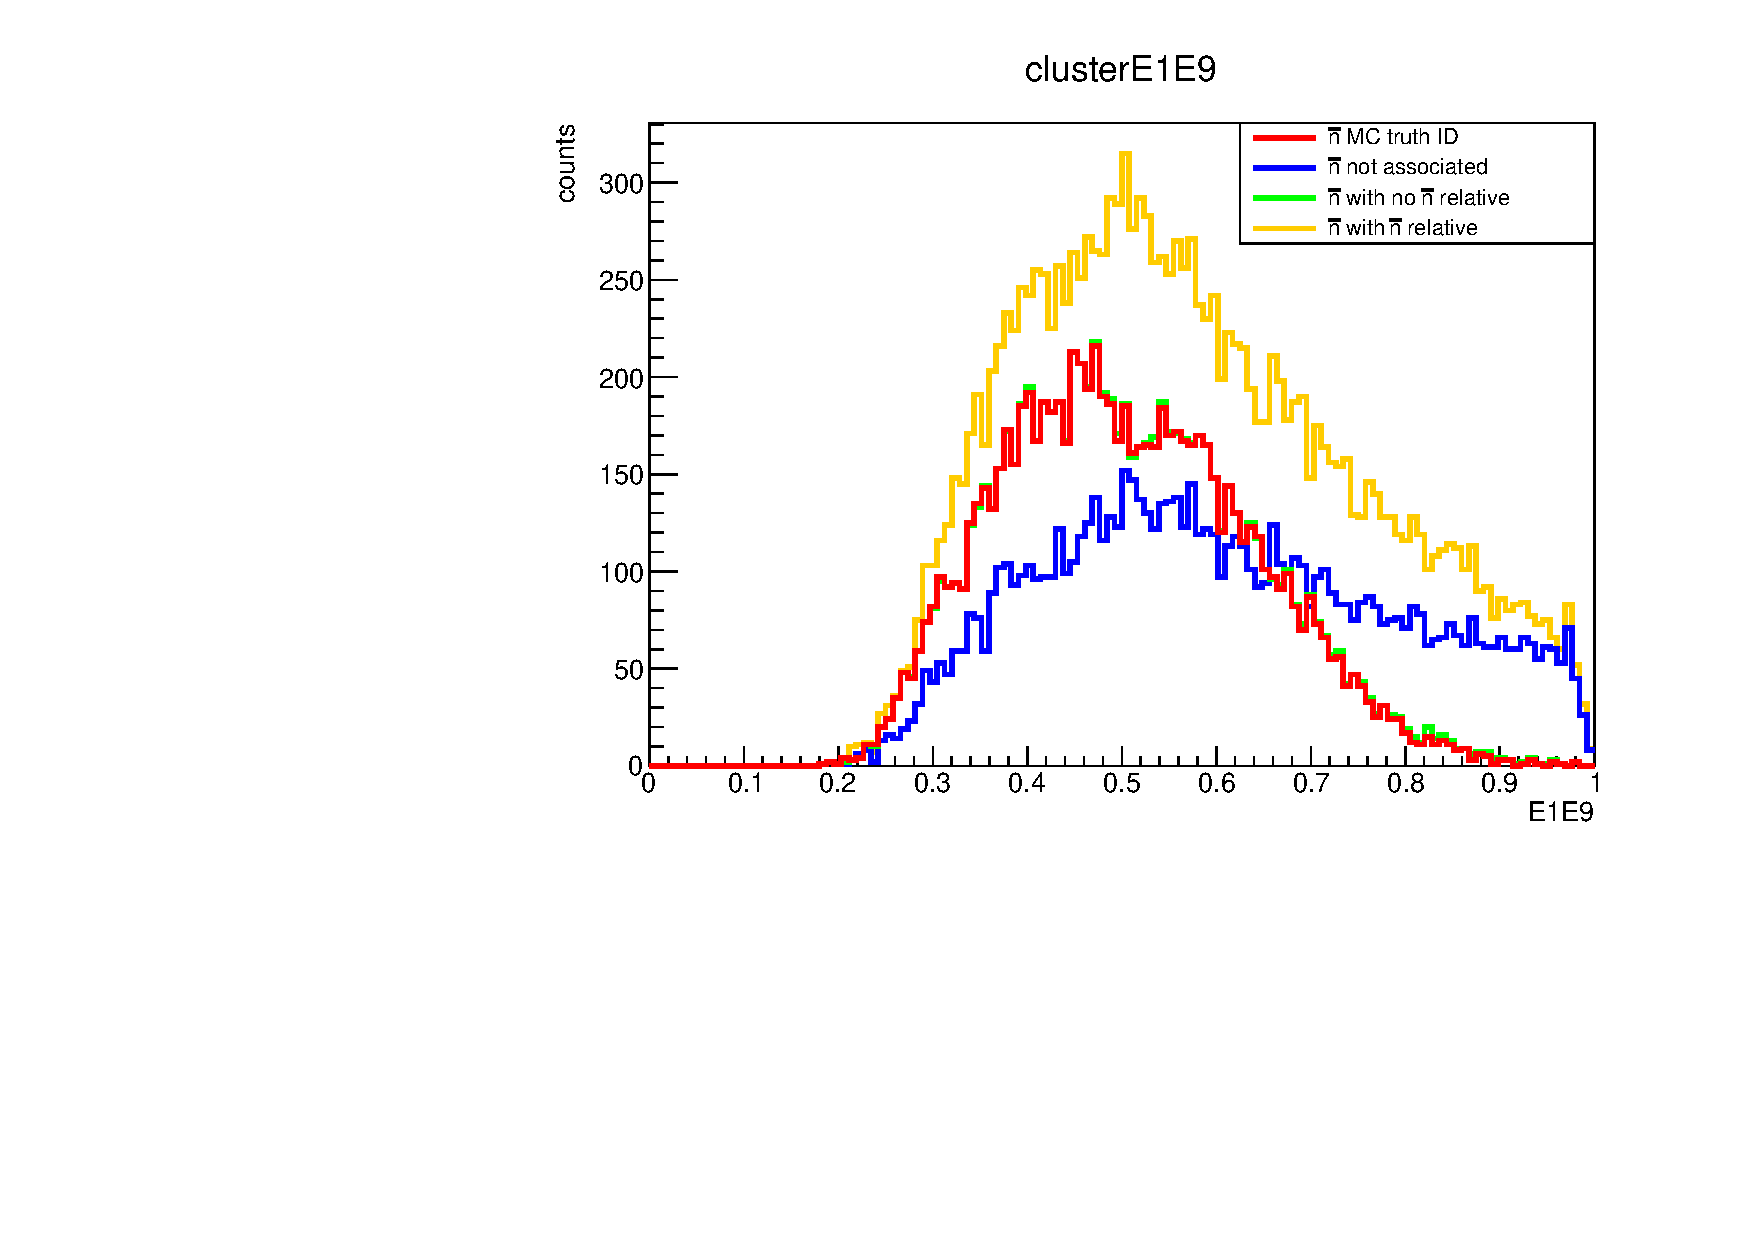
\includegraphics[width=0.49\textwidth]{nbar_MC/images/clusterE1E9_nog_ancestor.pdf}
    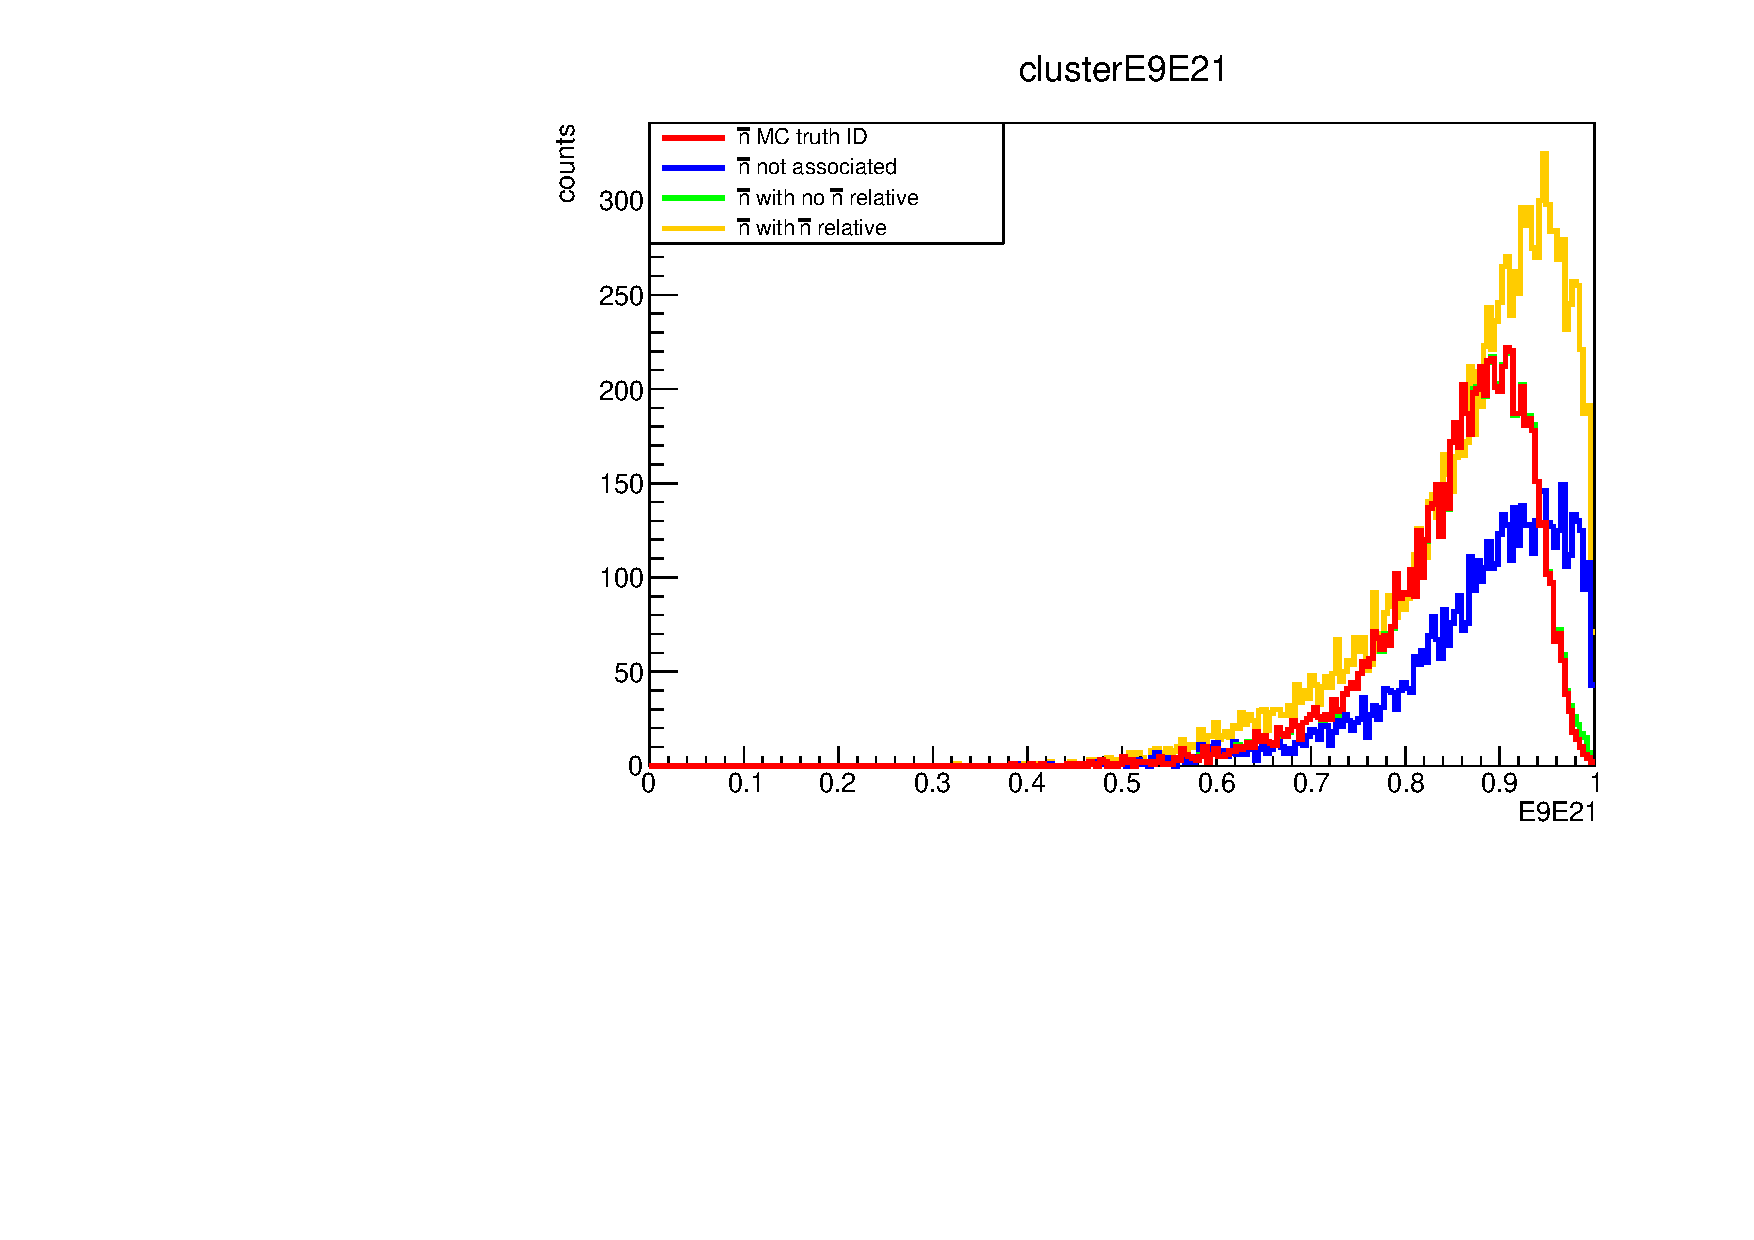
\includegraphics[width=0.49\textwidth]{nbar_MC/images/clusterE9E21_nog_ancestor.pdf}
    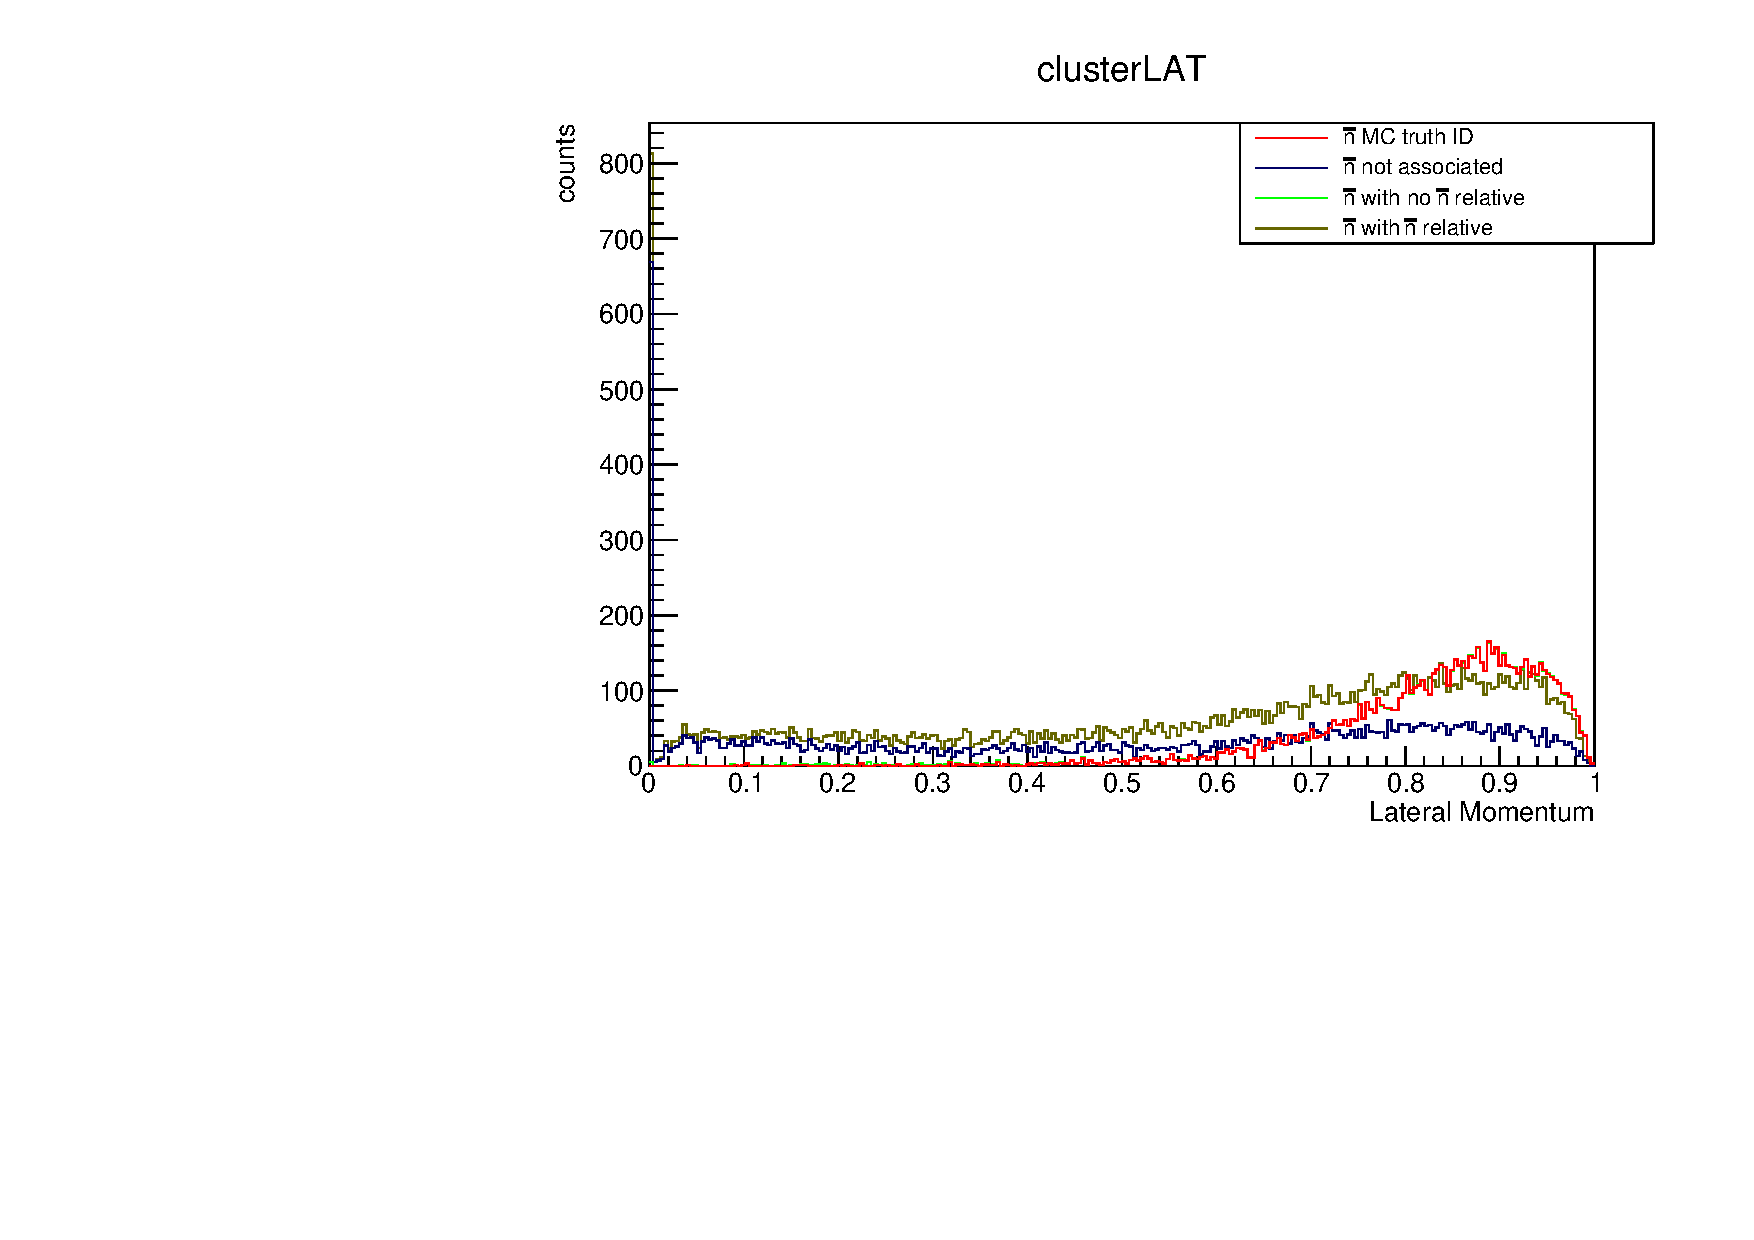
\includegraphics[width=0.49\textwidth]{nbar_MC/images/clusterLAT_nog_ancestor.pdf}
    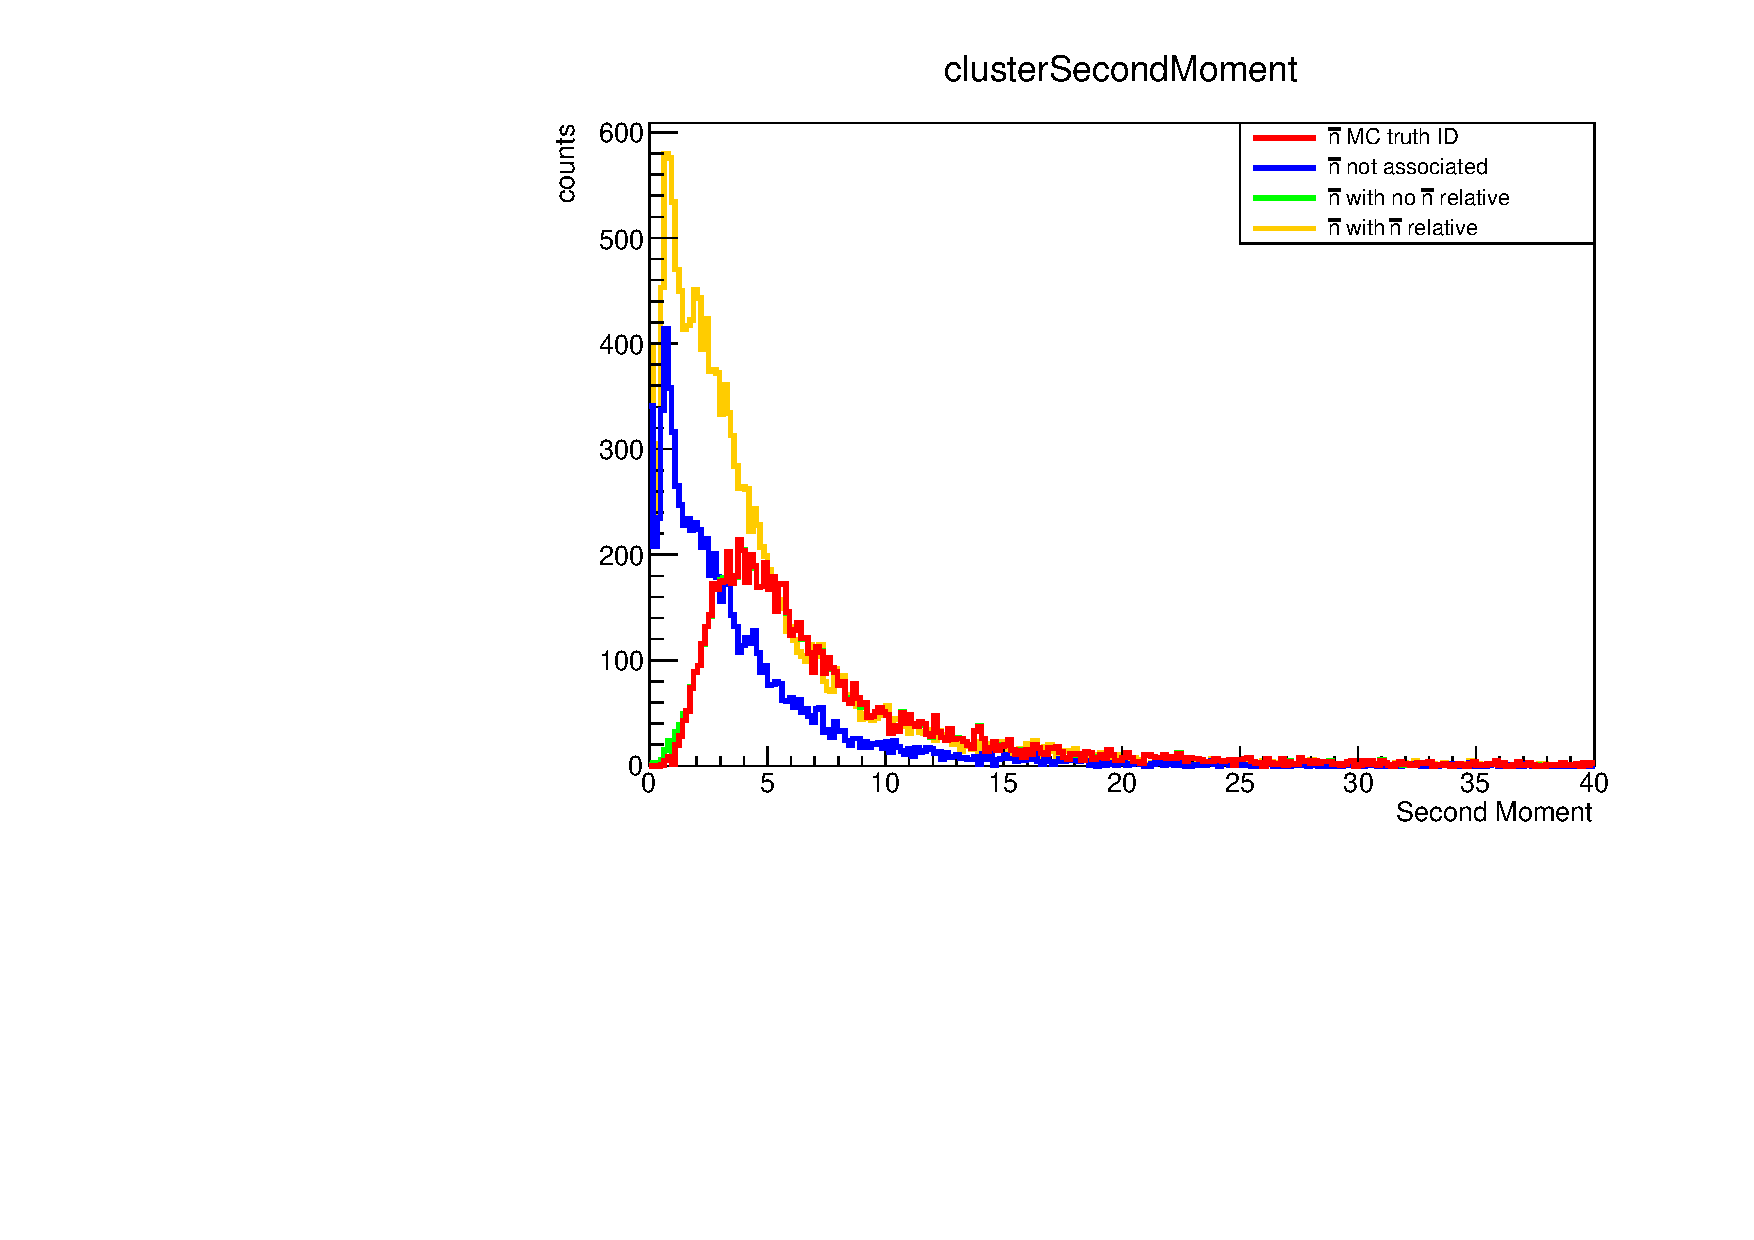
\includegraphics[width=0.49\textwidth]{nbar_MC/images/clusterSecondMoment_nog_ancestor.pdf}
    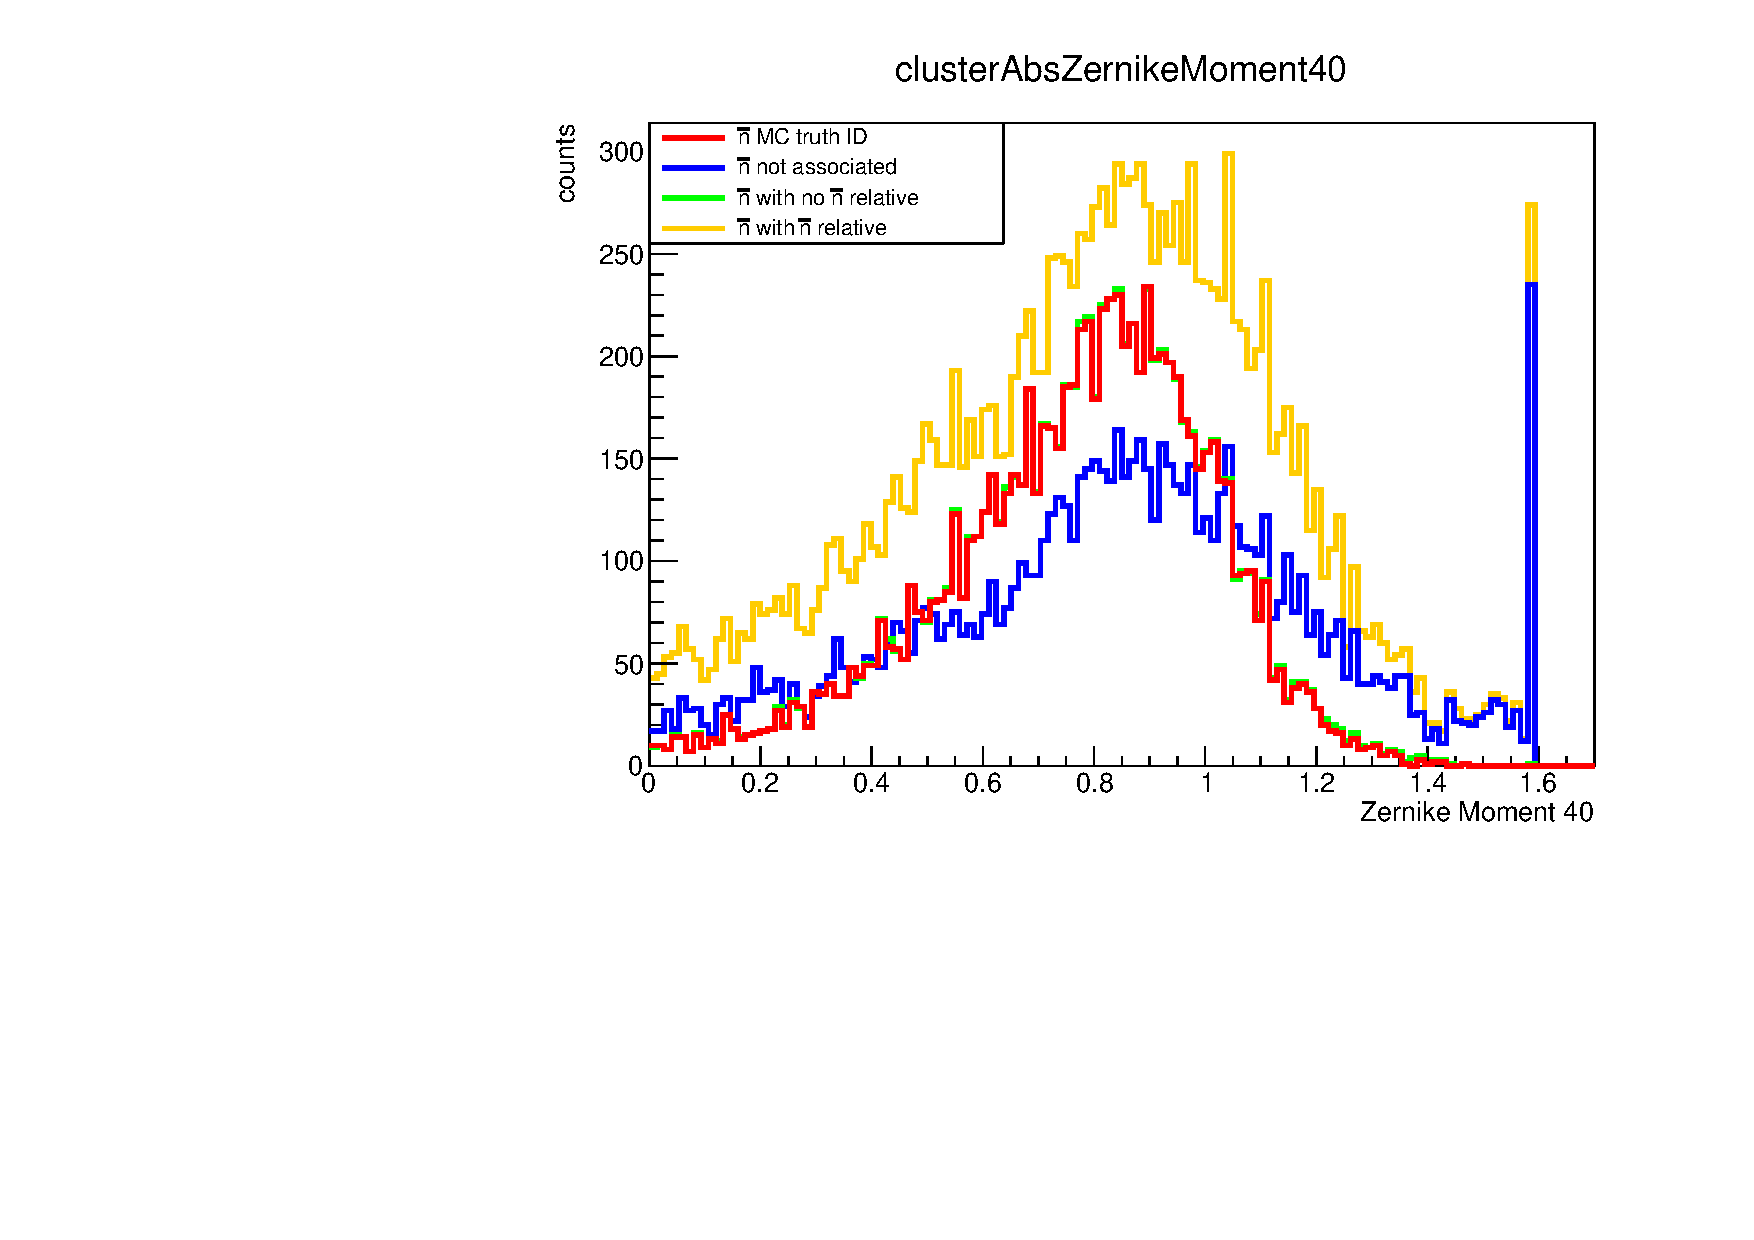
\includegraphics[width=0.49\textwidth]{nbar_MC/images/clusterAbsZernikeMoment40_nog_ancestor.pdf}
    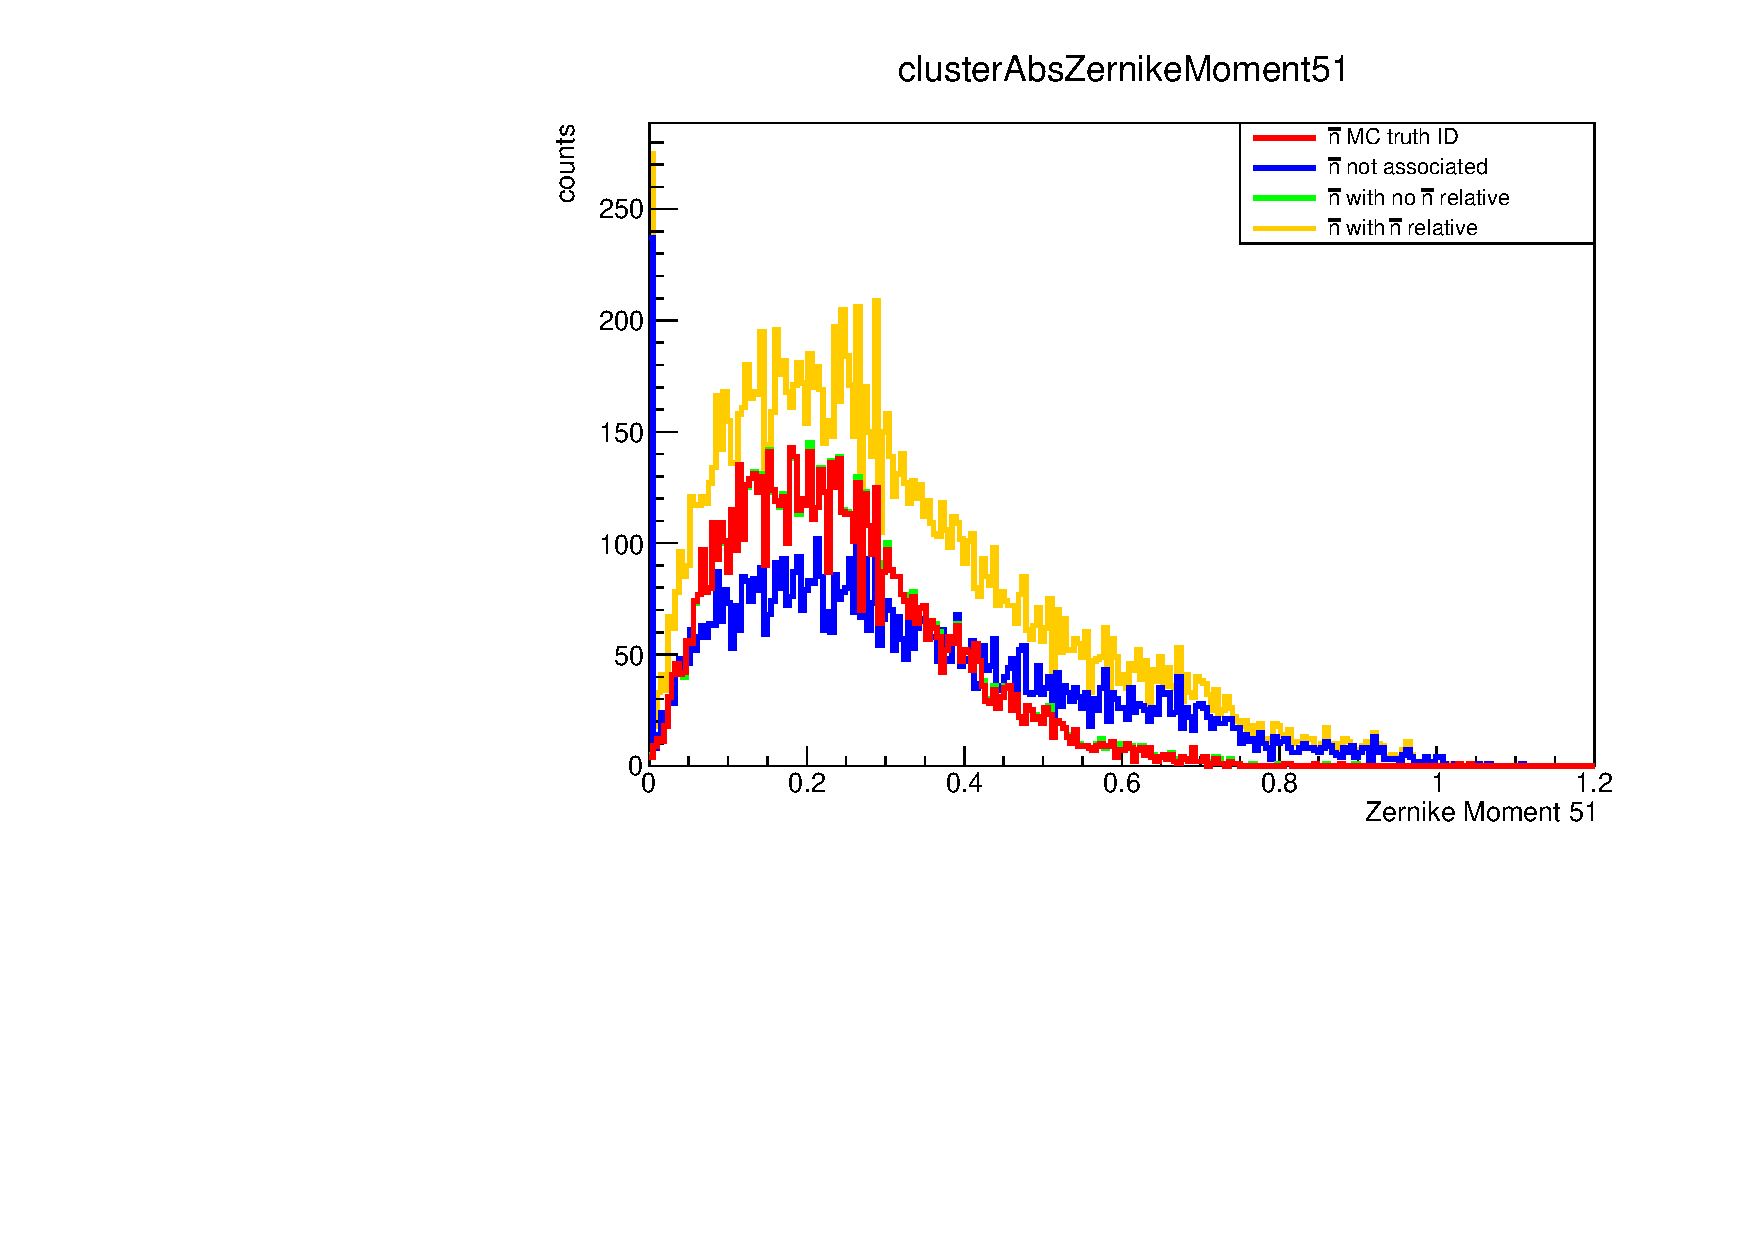
\includegraphics[width=0.49\textwidth]{nbar_MC/images/clusterAbsZernikeMoment51_nog_ancestor.pdf}
    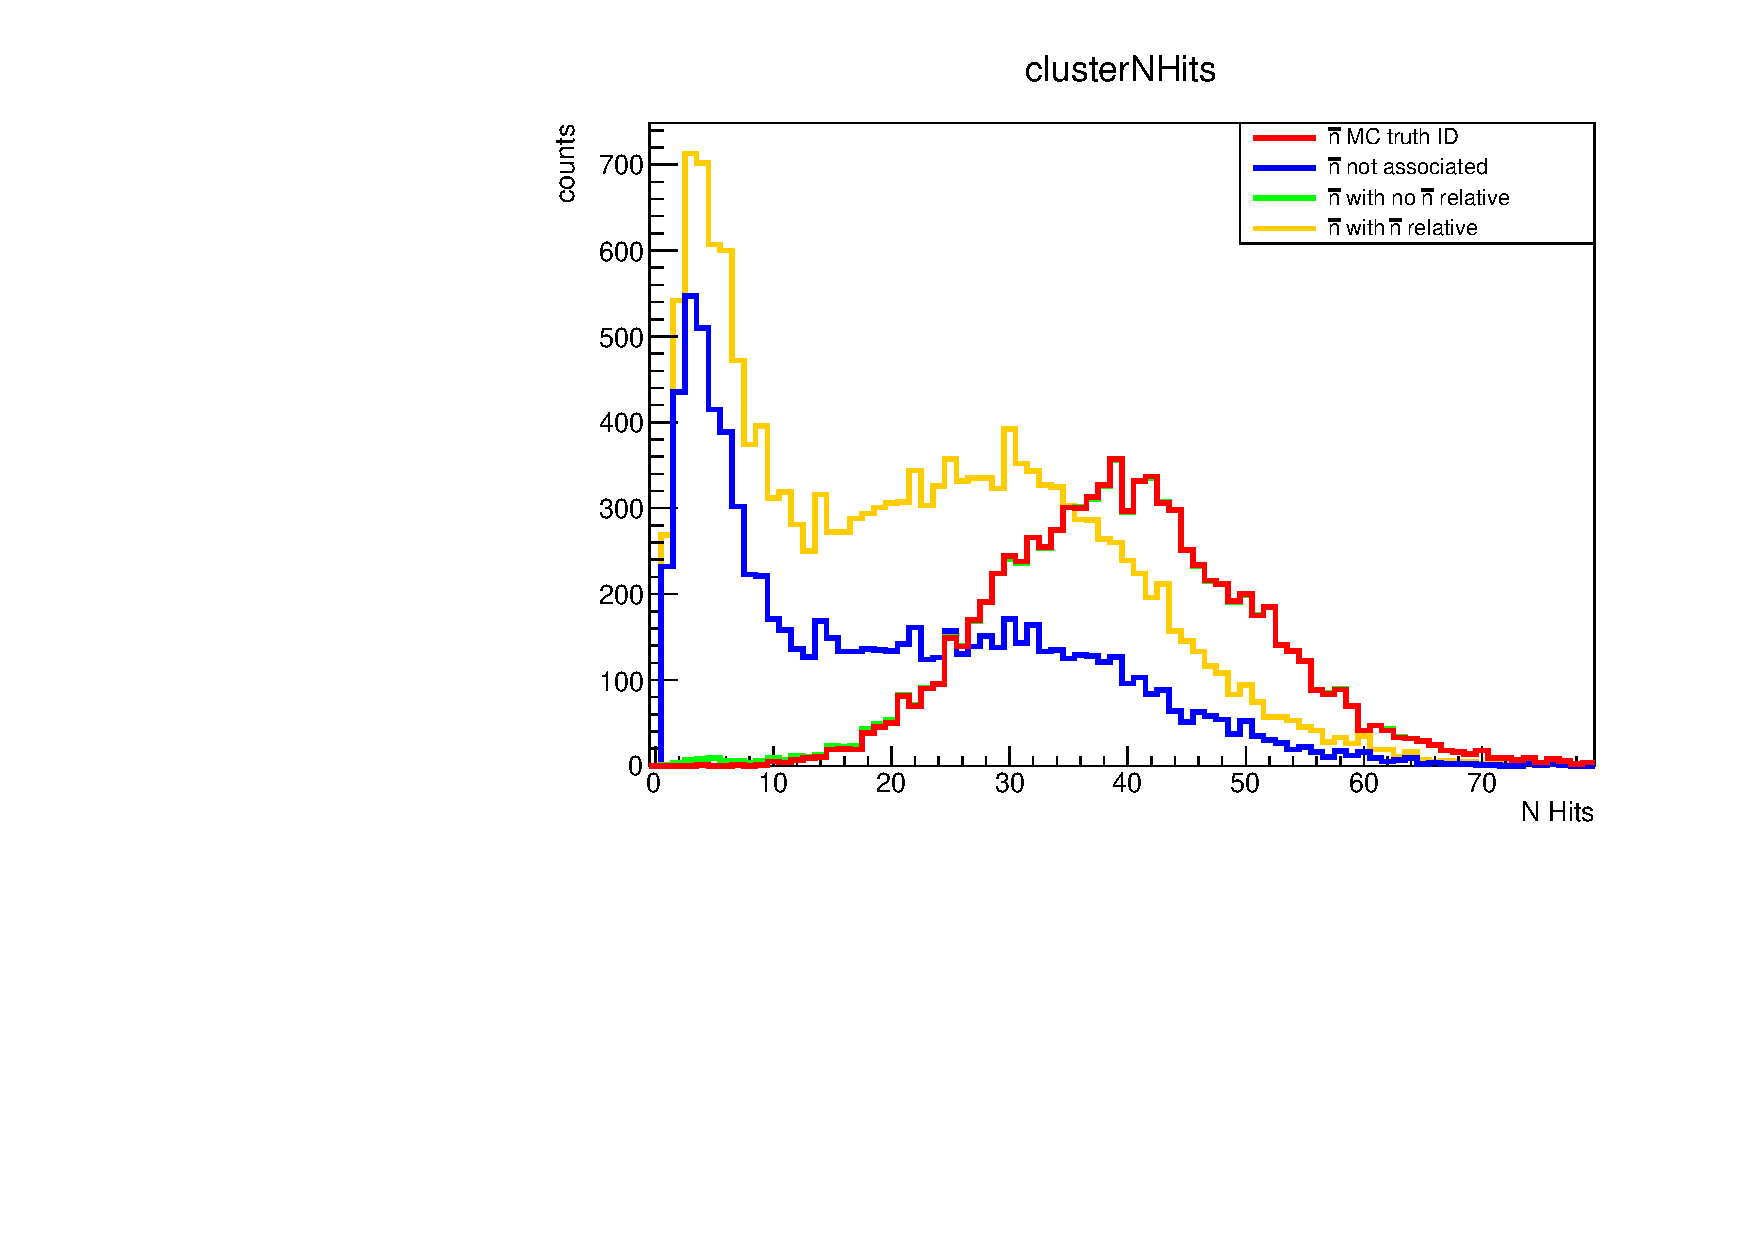
\includegraphics[width=0.49\textwidth]{nbar_MC/images/clusterNHits_nog_ancestor.pdf}
   
     \caption{Comparison of reconstructed cluster variables for $\bar{n}$ candidates with different ancestor selection (NO ISR case)}
     \label{fig:cluster_NOISR}

\end{figure}


\newpage
The obtained cluster variables in ISR case are shown below:
 \begin{figure}[H]
    \centering
    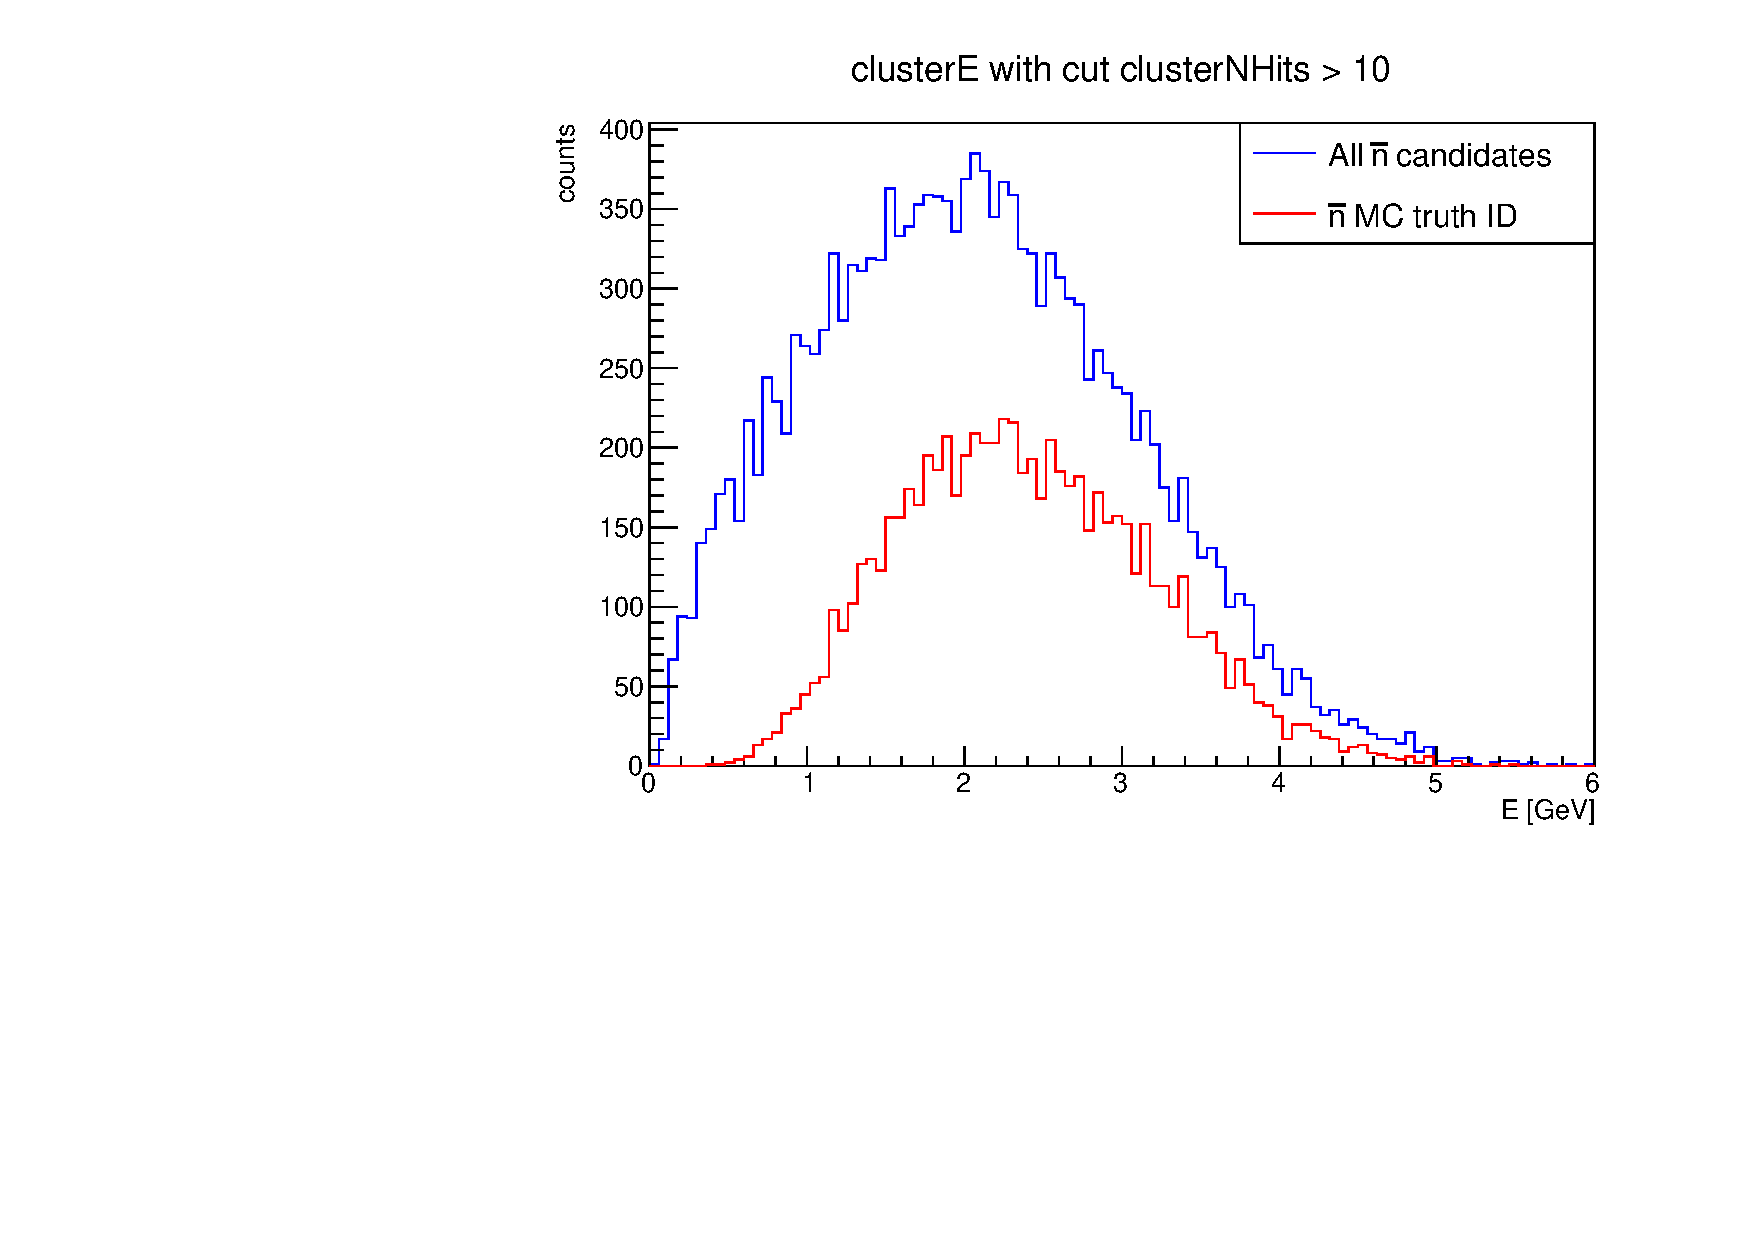
\includegraphics[width=0.49\textwidth]{nbar_MC/images/clusterE_hitscut_isr.pdf}
    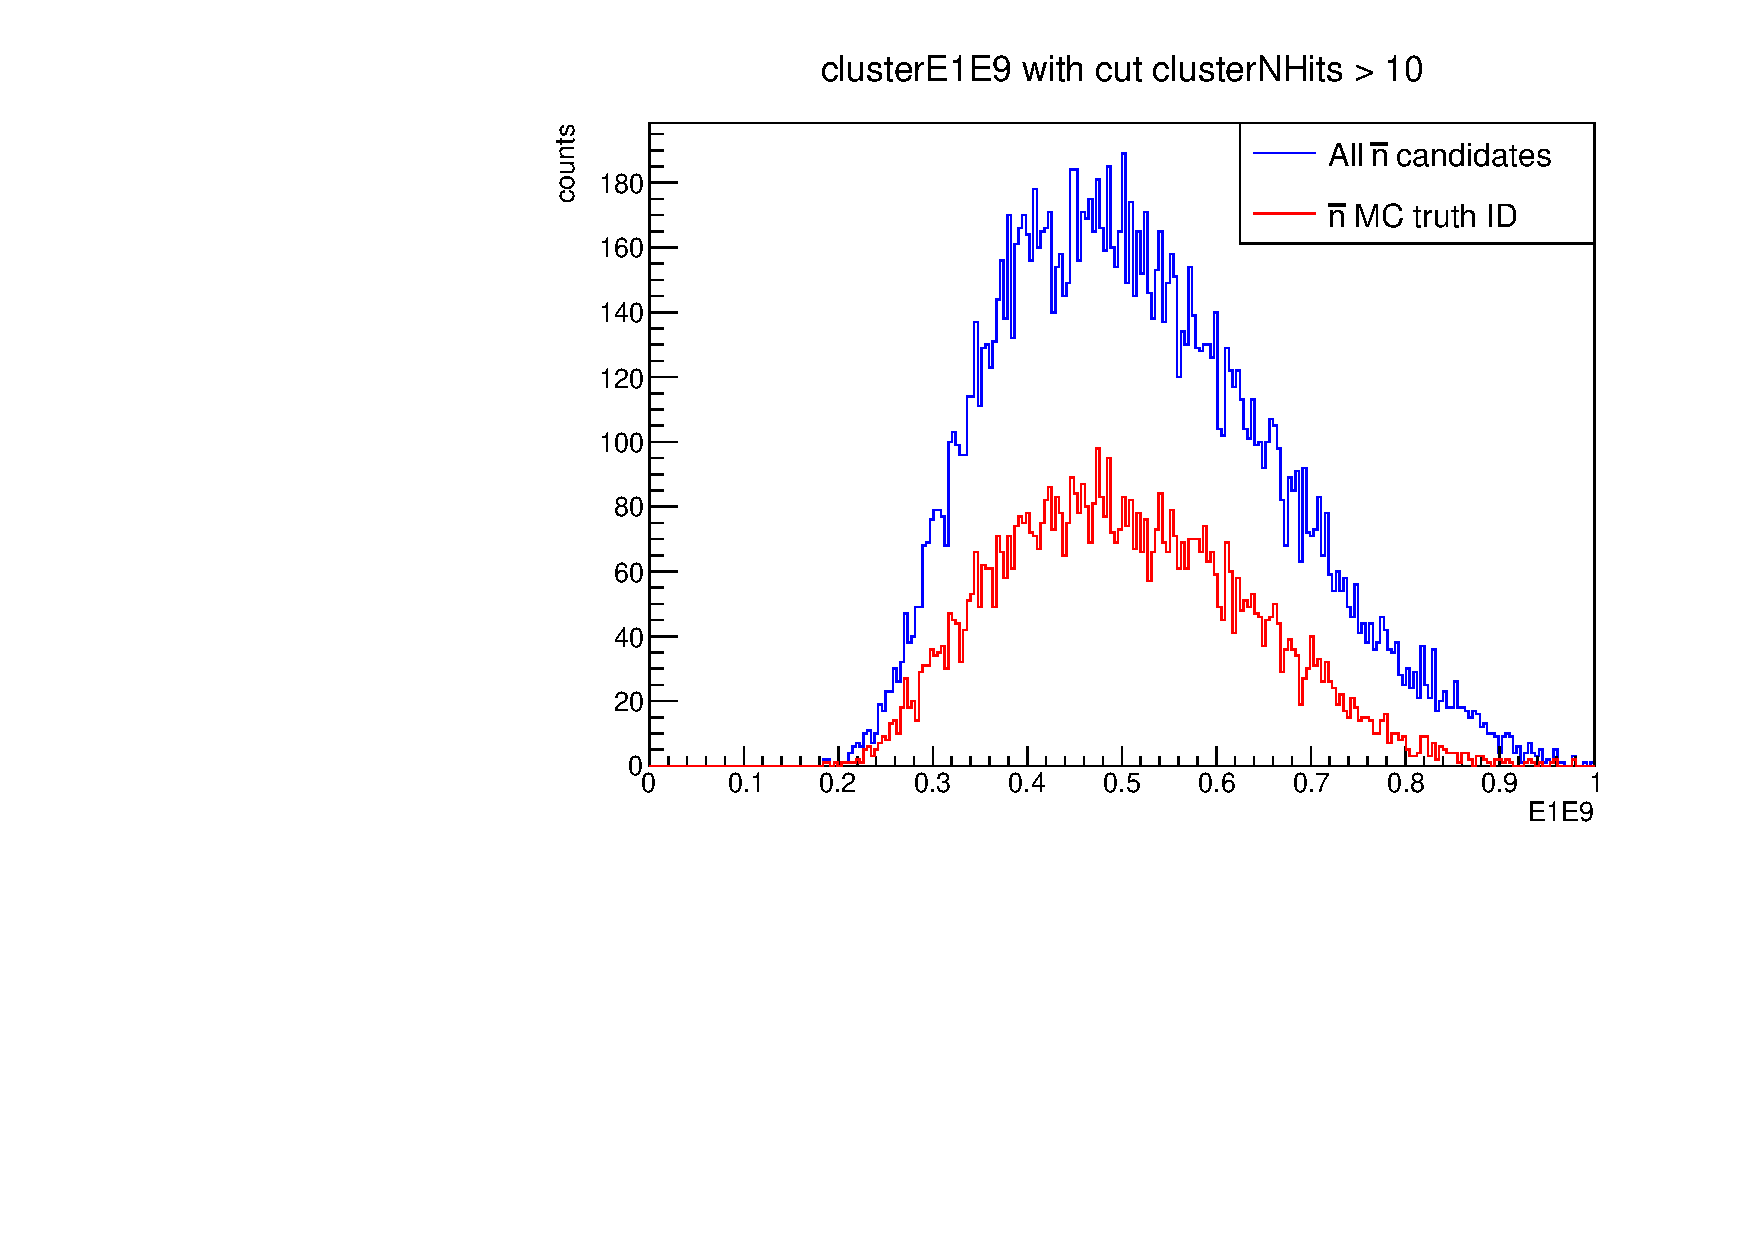
\includegraphics[width=0.49\textwidth]{nbar_MC/images/clusterE1E9_hitscut_isr.pdf}
    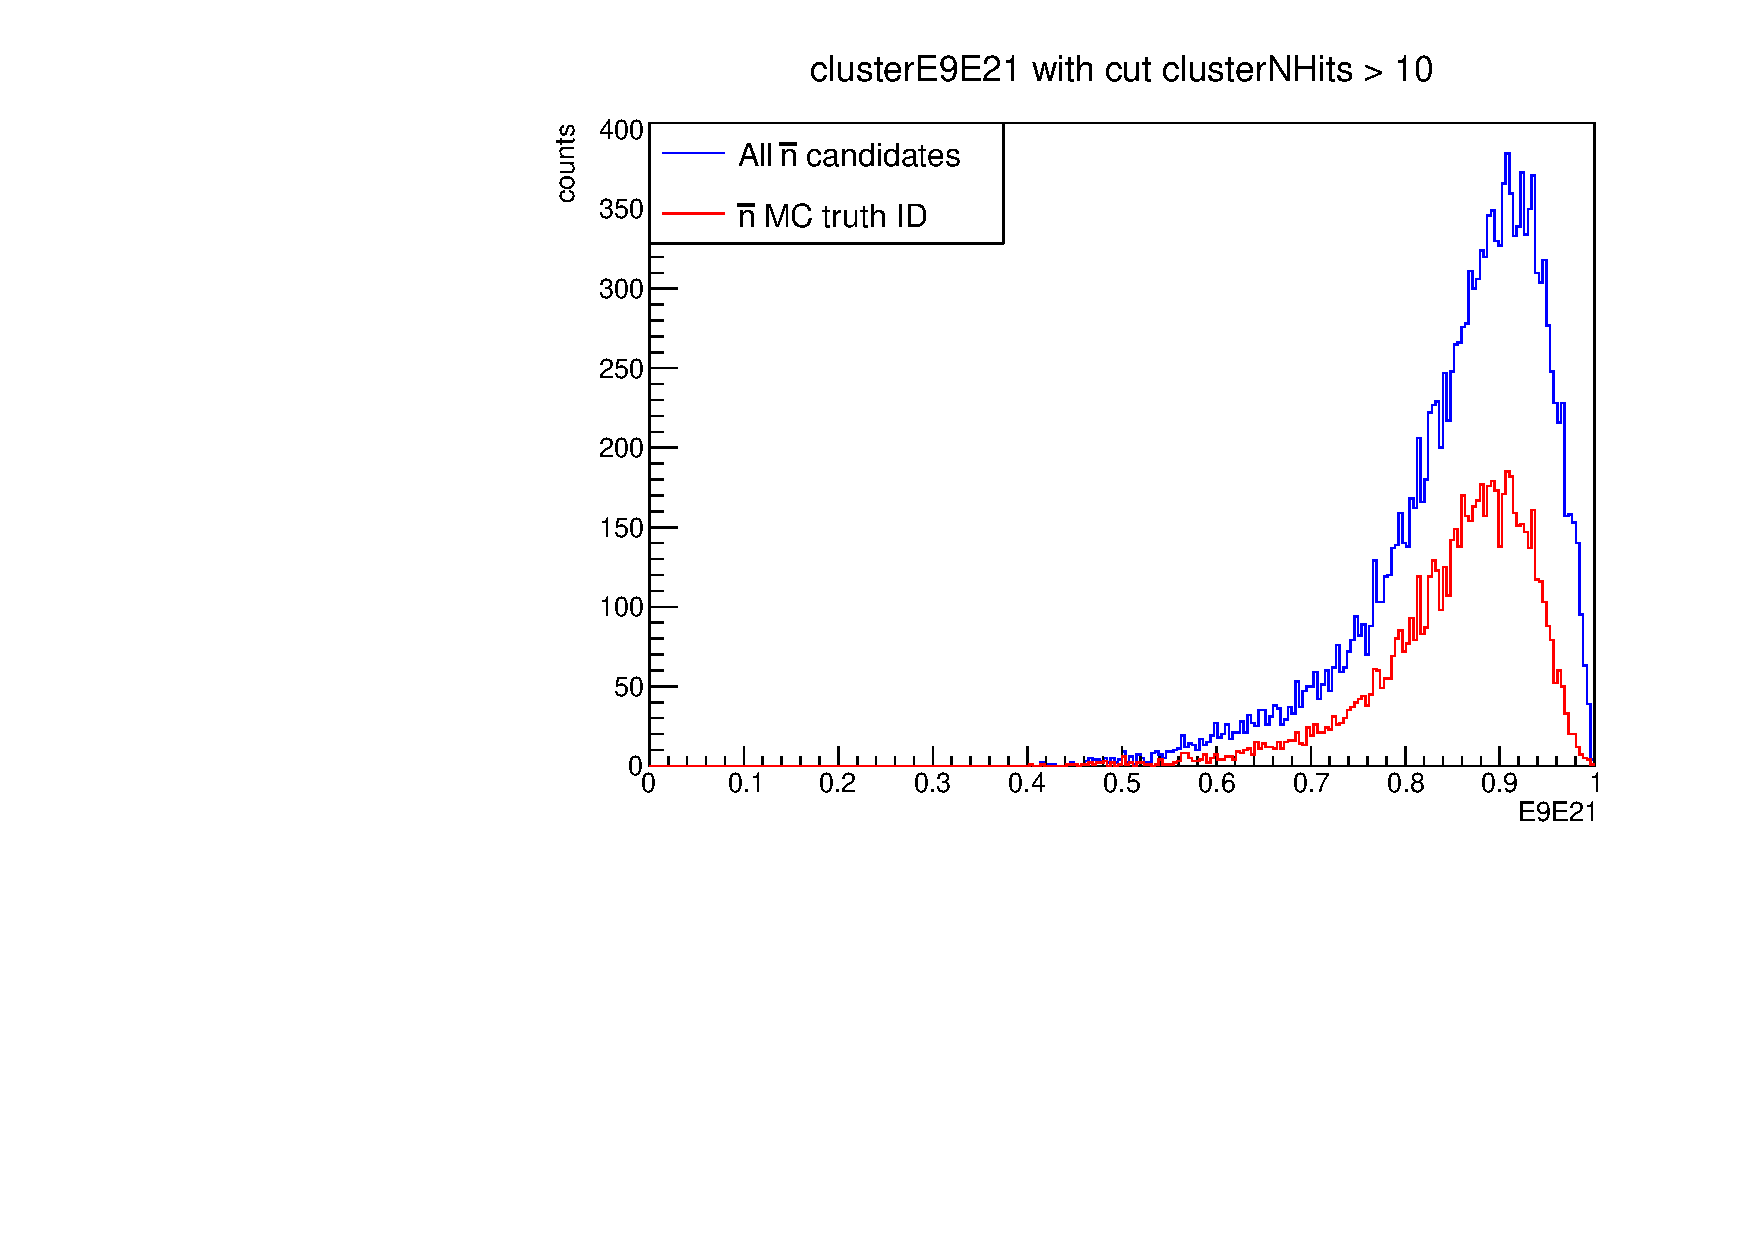
\includegraphics[width=0.49\textwidth]{nbar_MC/images/clusterE9E21_hitscut_isr.pdf}
    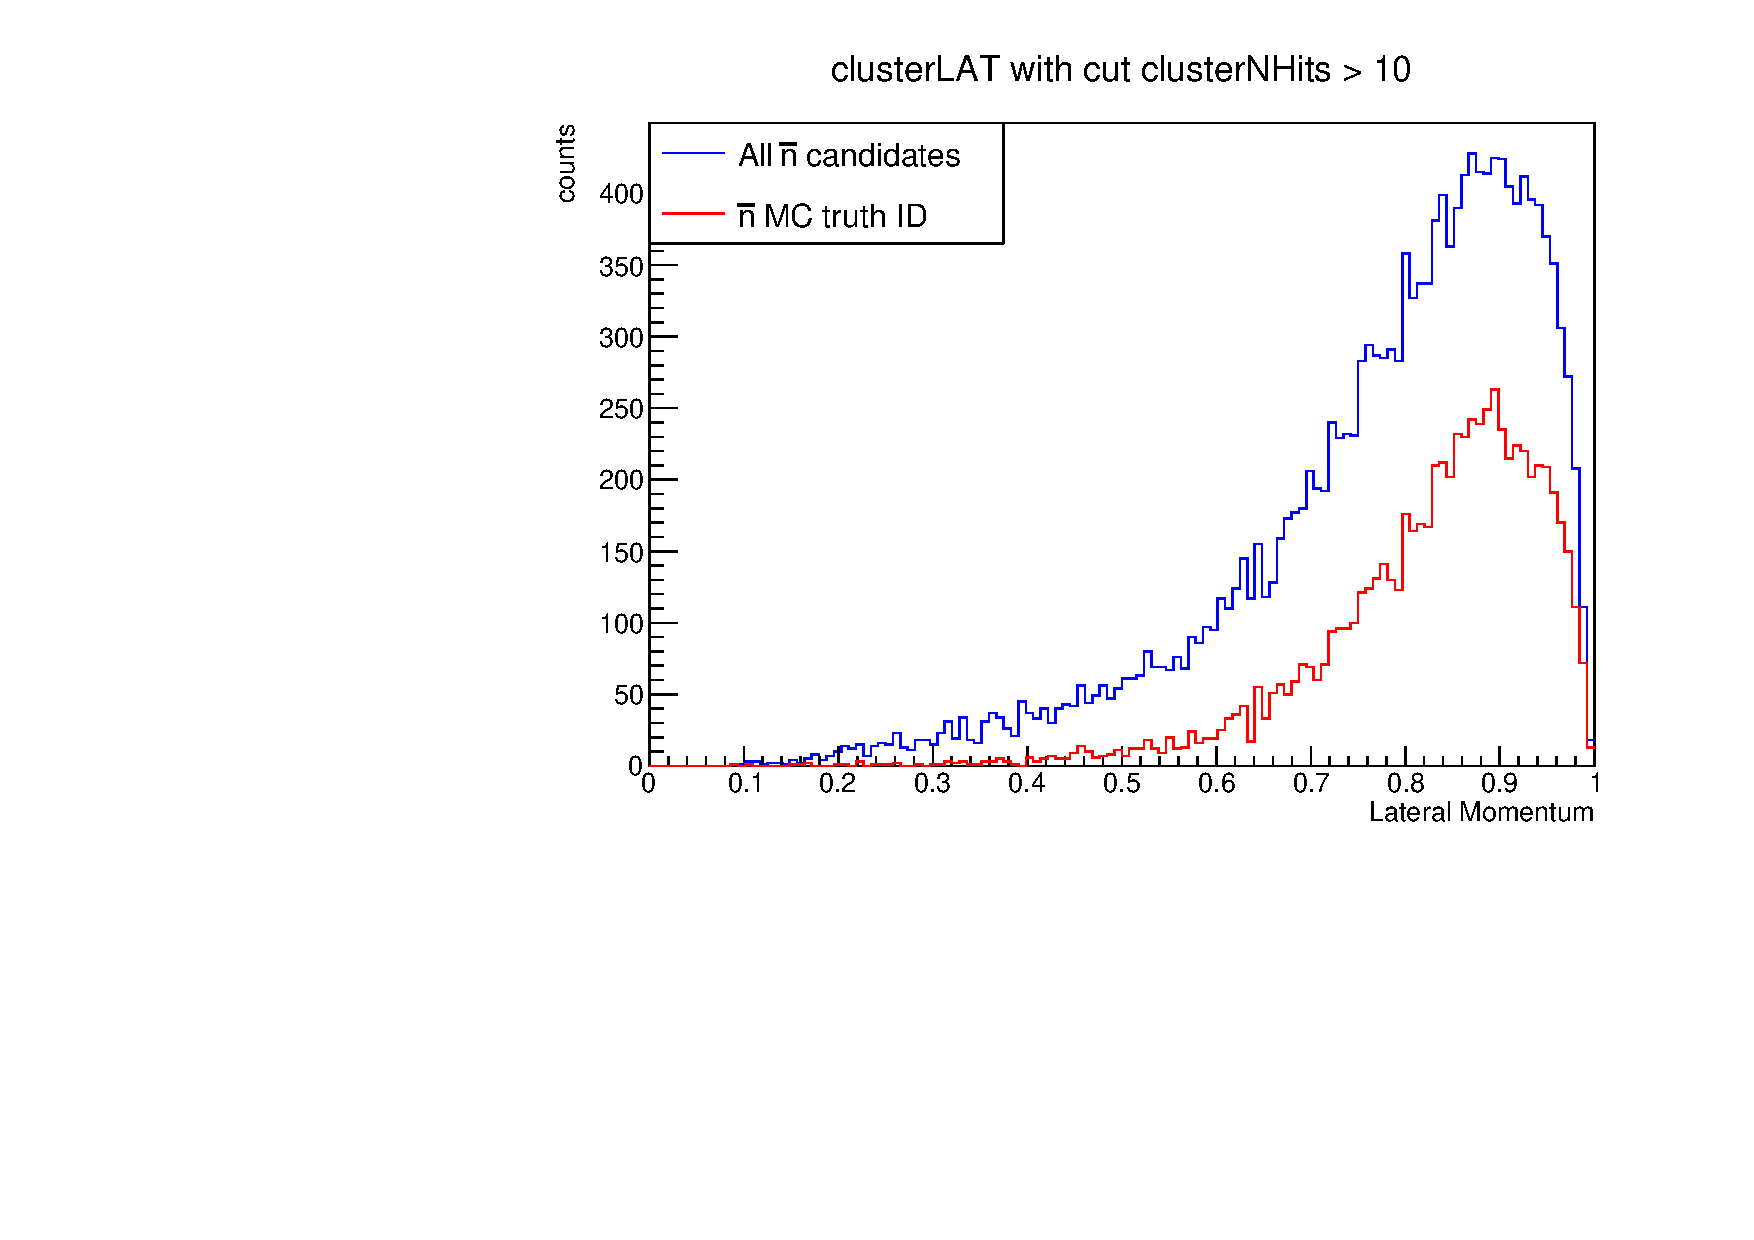
\includegraphics[width=0.49\textwidth]{nbar_MC/images/clusterLAT_hitscut_isr.pdf}
    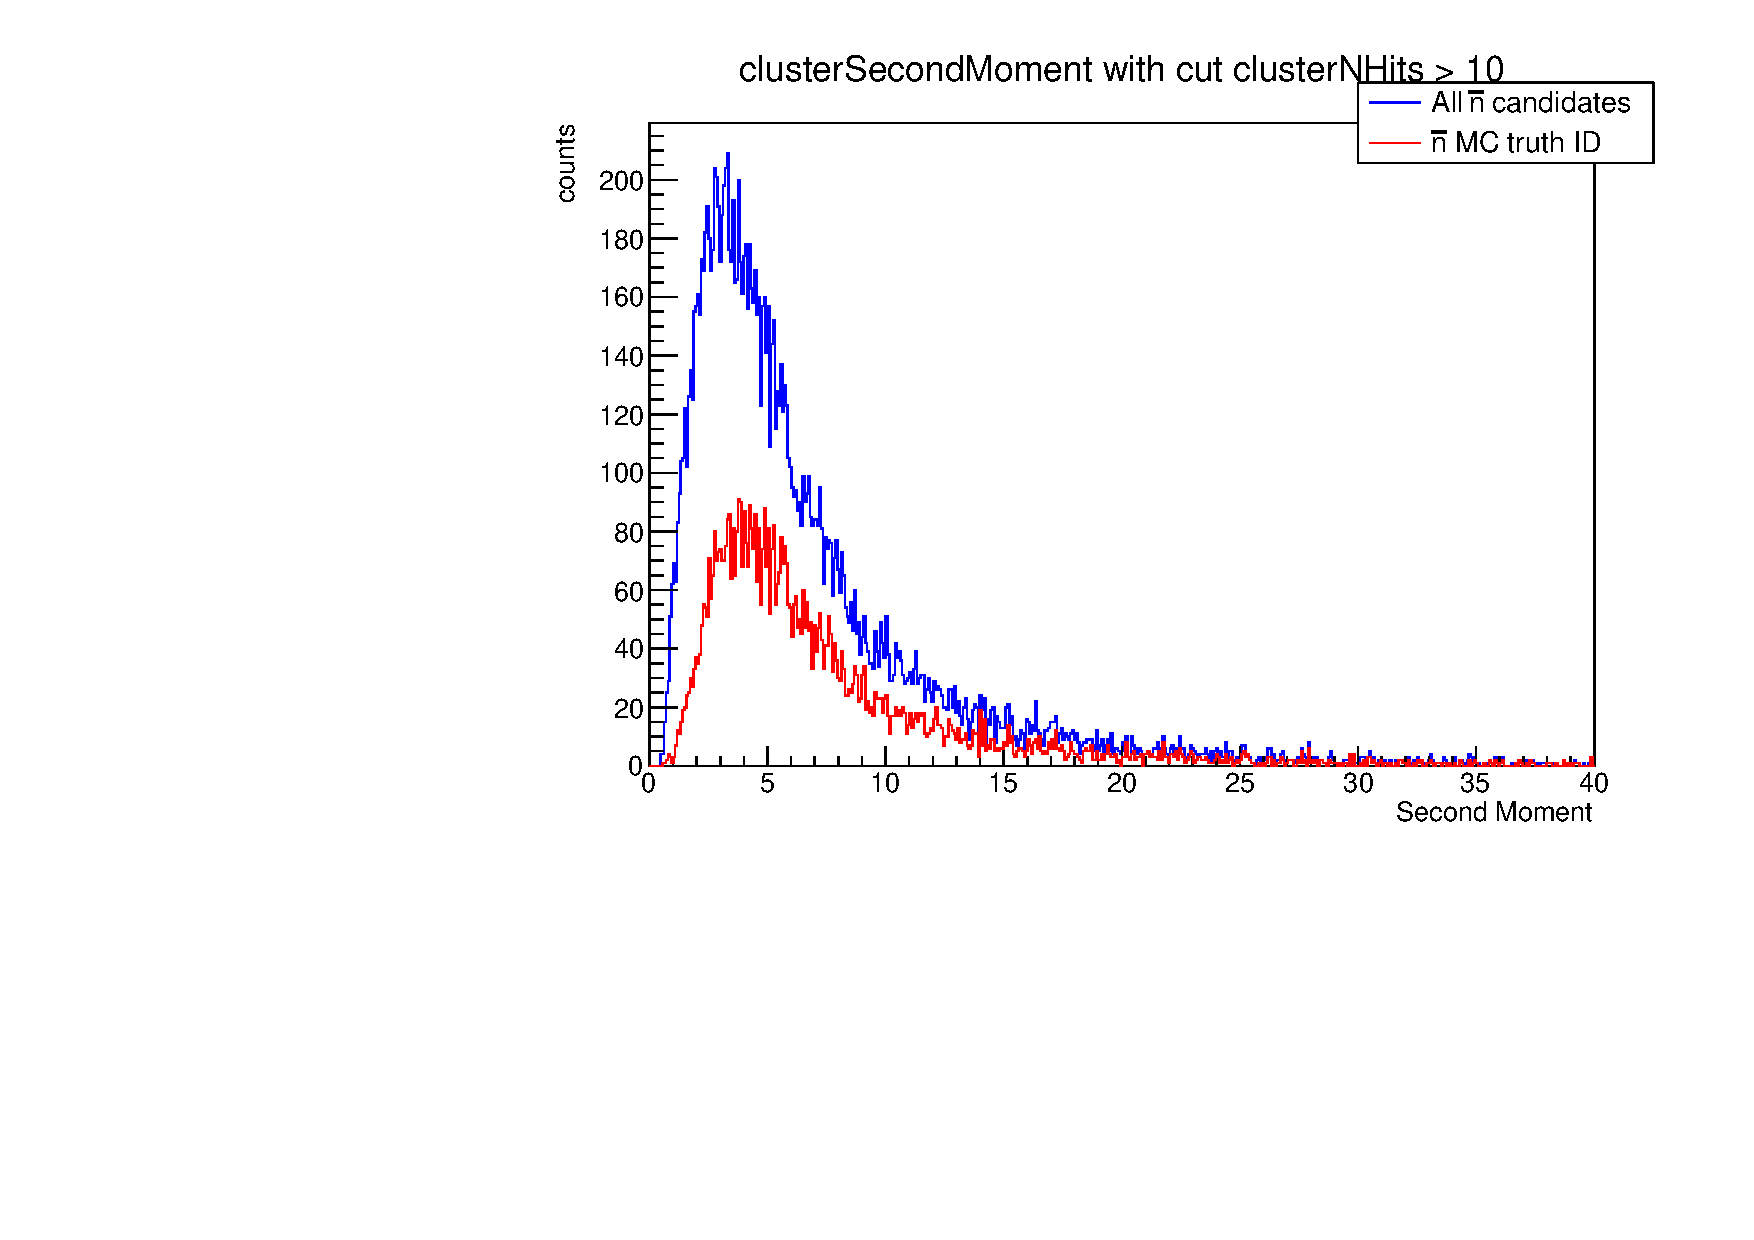
\includegraphics[width=0.49\textwidth]{nbar_MC/images/clusterSecondMoment_hitscut_isr.pdf}
    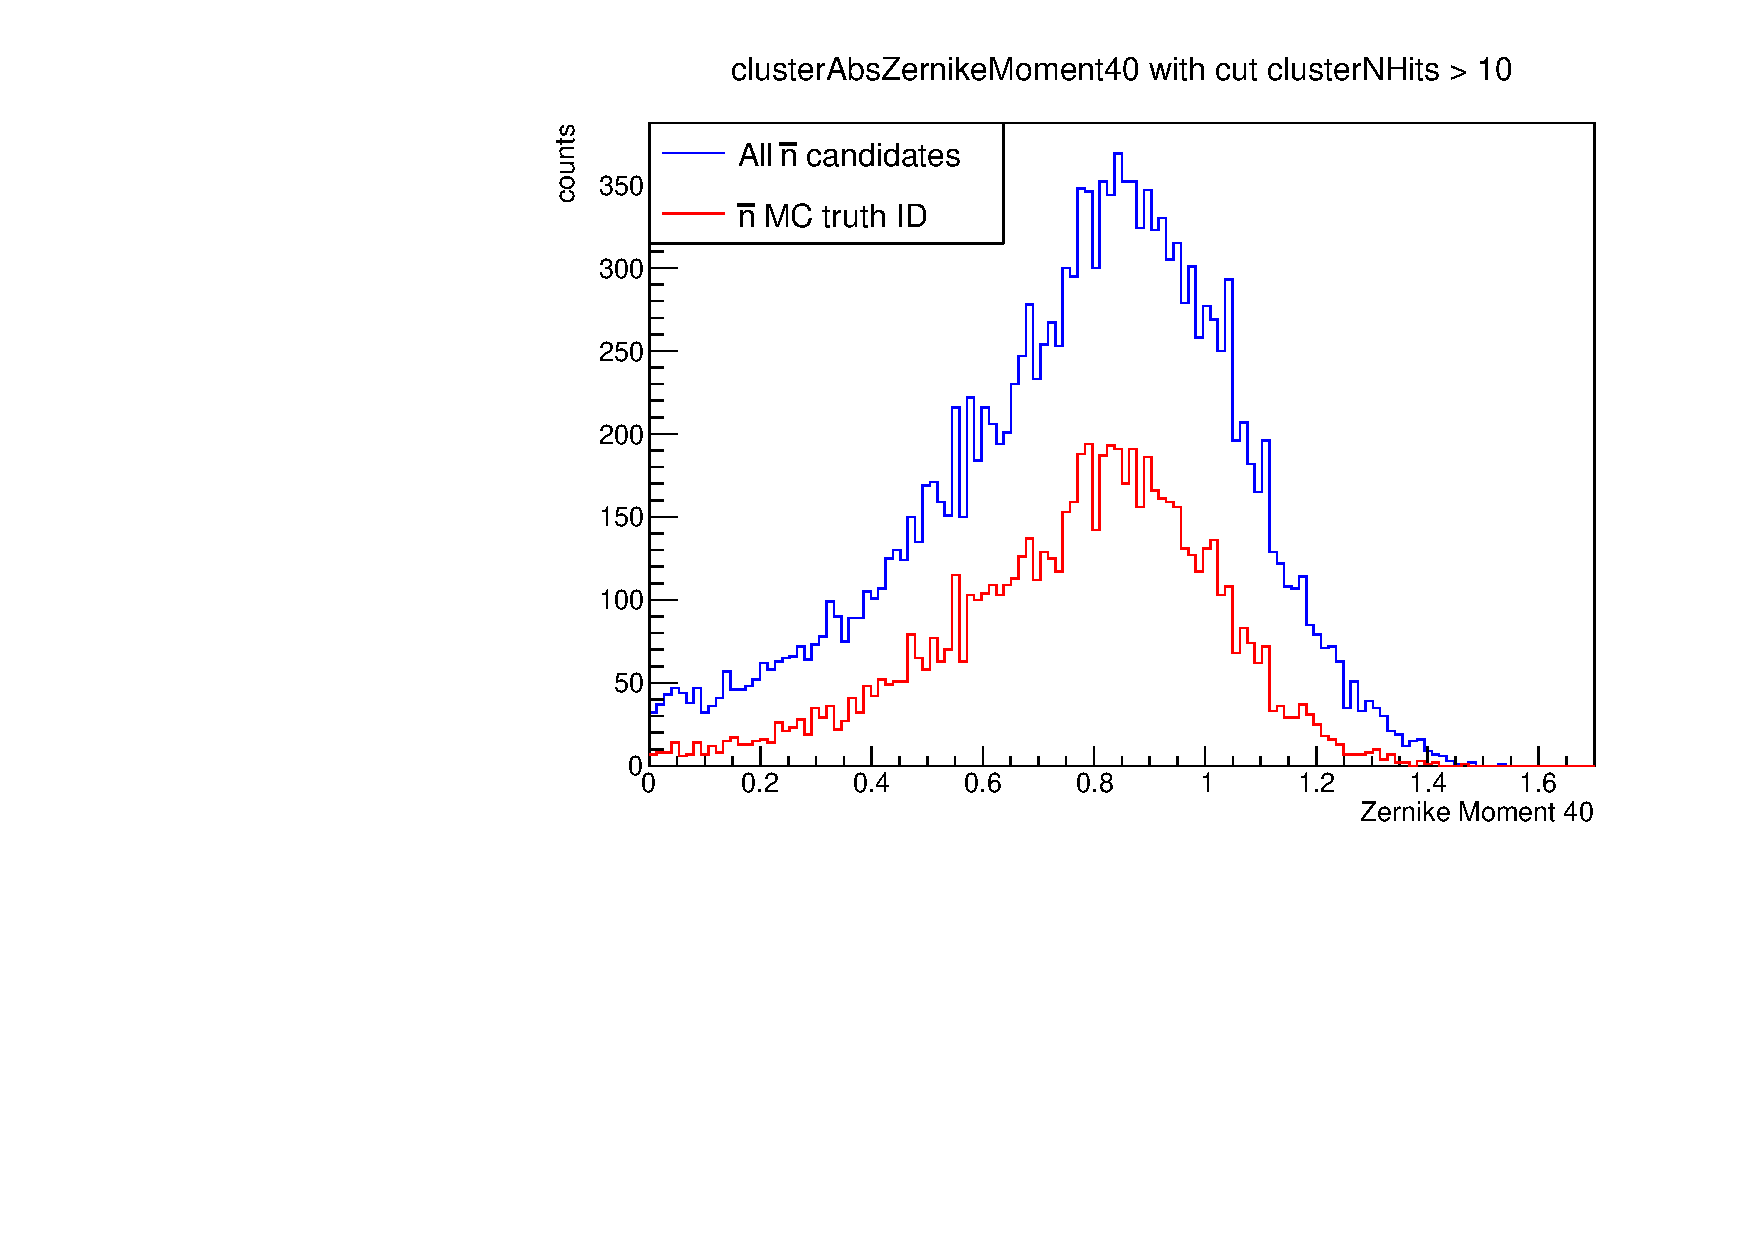
\includegraphics[width=0.49\textwidth]{nbar_MC/images/clusterAbsZernikeMoment40_hitscut_isr.pdf}
    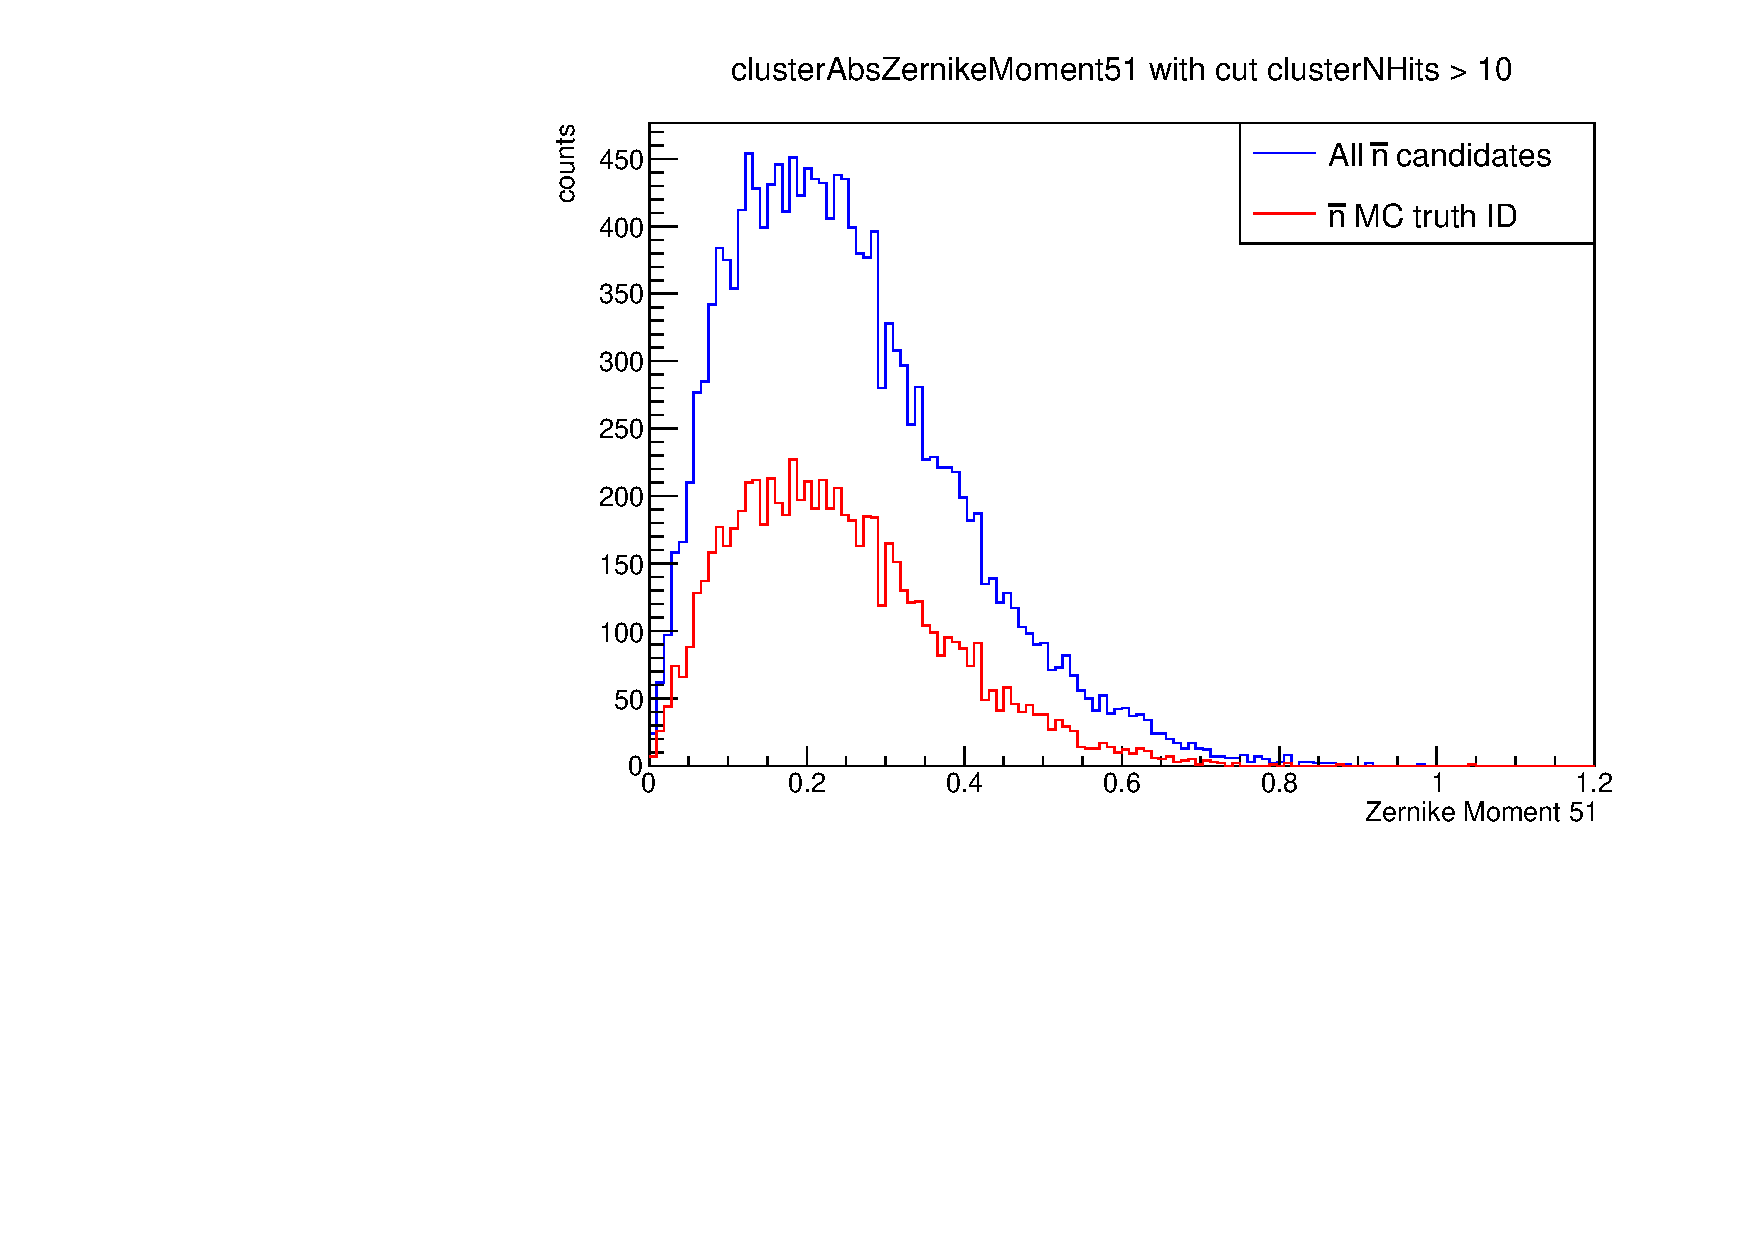
\includegraphics[width=0.49\textwidth]{nbar_MC/images/clusterAbsZernikeMoment51_hitscut_isr.pdf}
    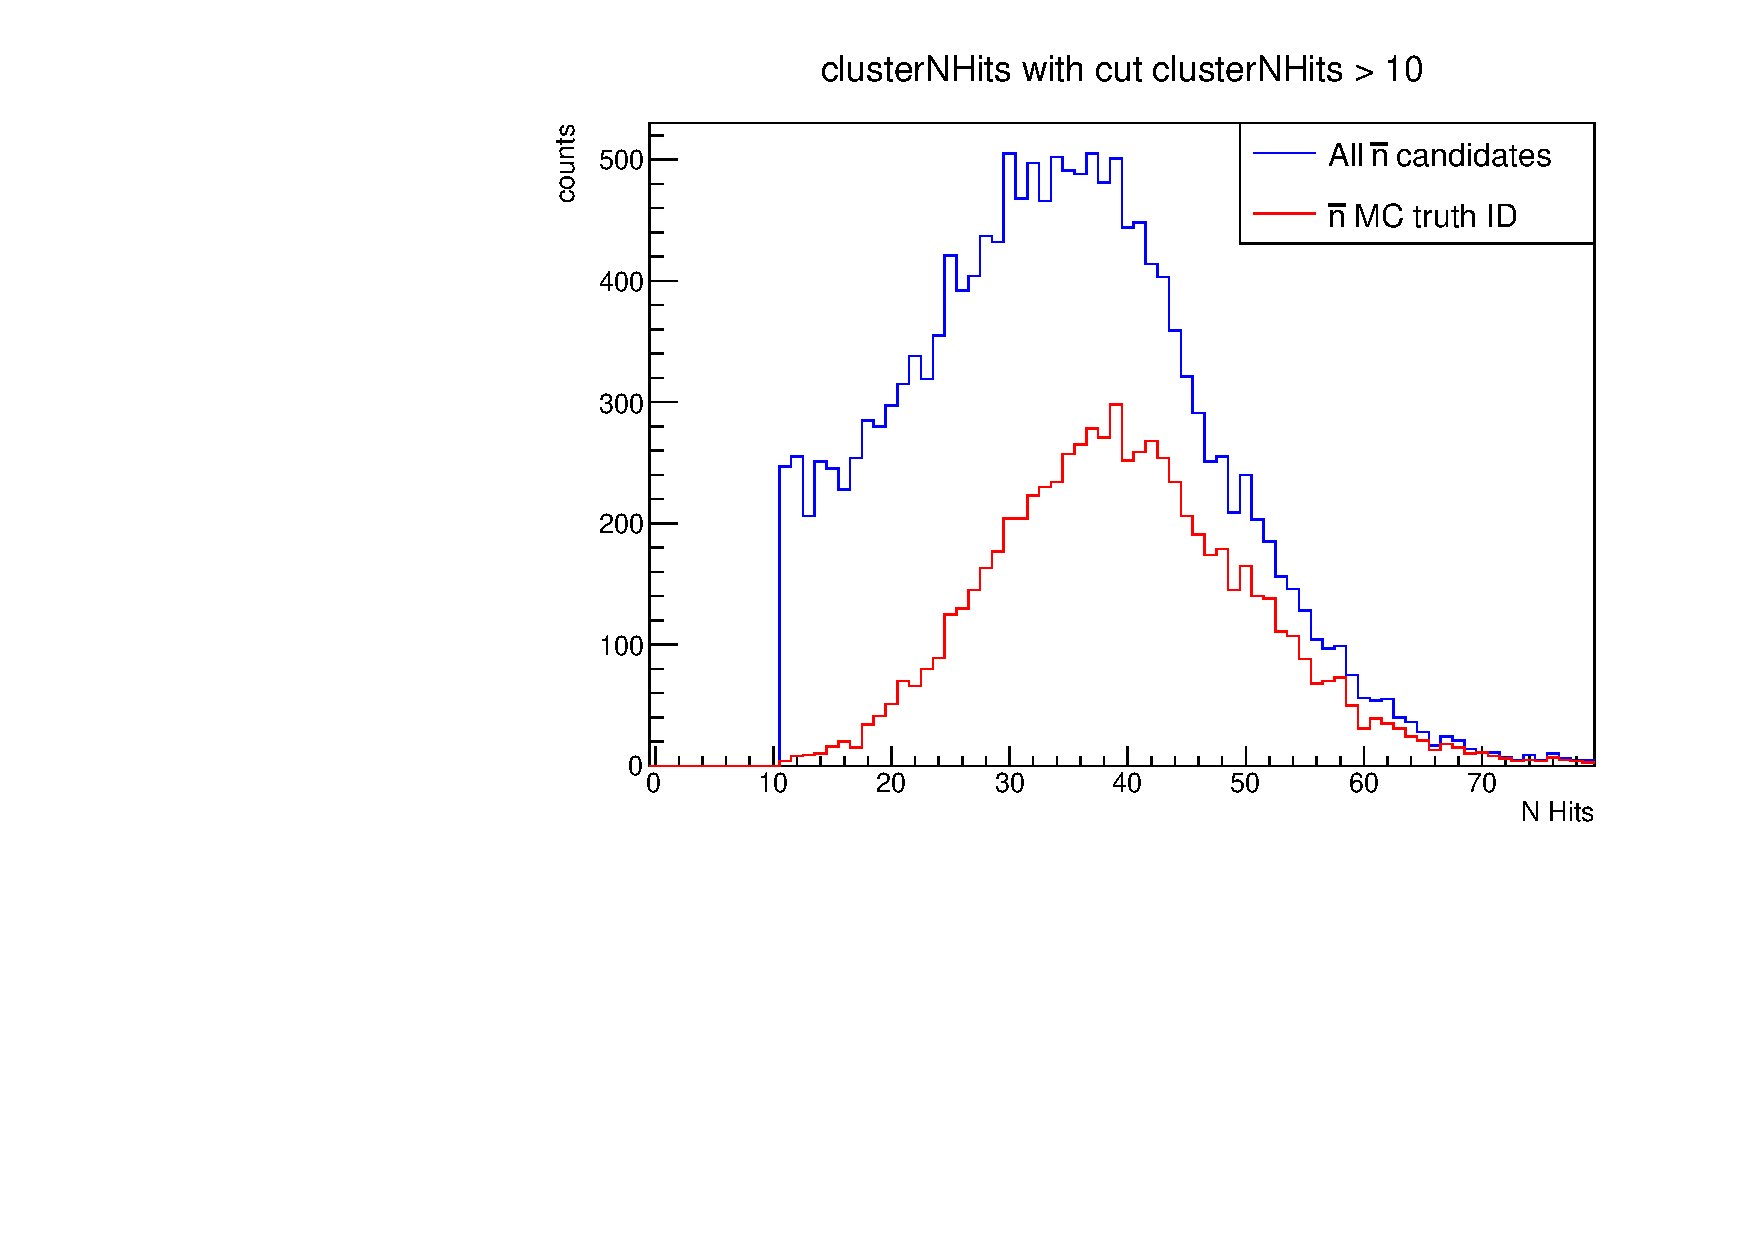
\includegraphics[width=0.49\textwidth]{nbar_MC/images/clusterNHits_hitscut_isr.pdf}
   
     \caption{Comparison of reconstructed cluster variables for all $\bar{n}$ candidates versus those associated with $\bar{n}$ particles by Monte Carlo truth Monte Carlo PDG = -2112 (ISR case). Cut $clusterNHits > 10$ is performed}
     
     \label{fig:cluster_ISR_NHits}

\end{figure}

\newpage
The obtained cluster variables in NO ISR case are shown below:
 \begin{figure}[H]
    \centering
    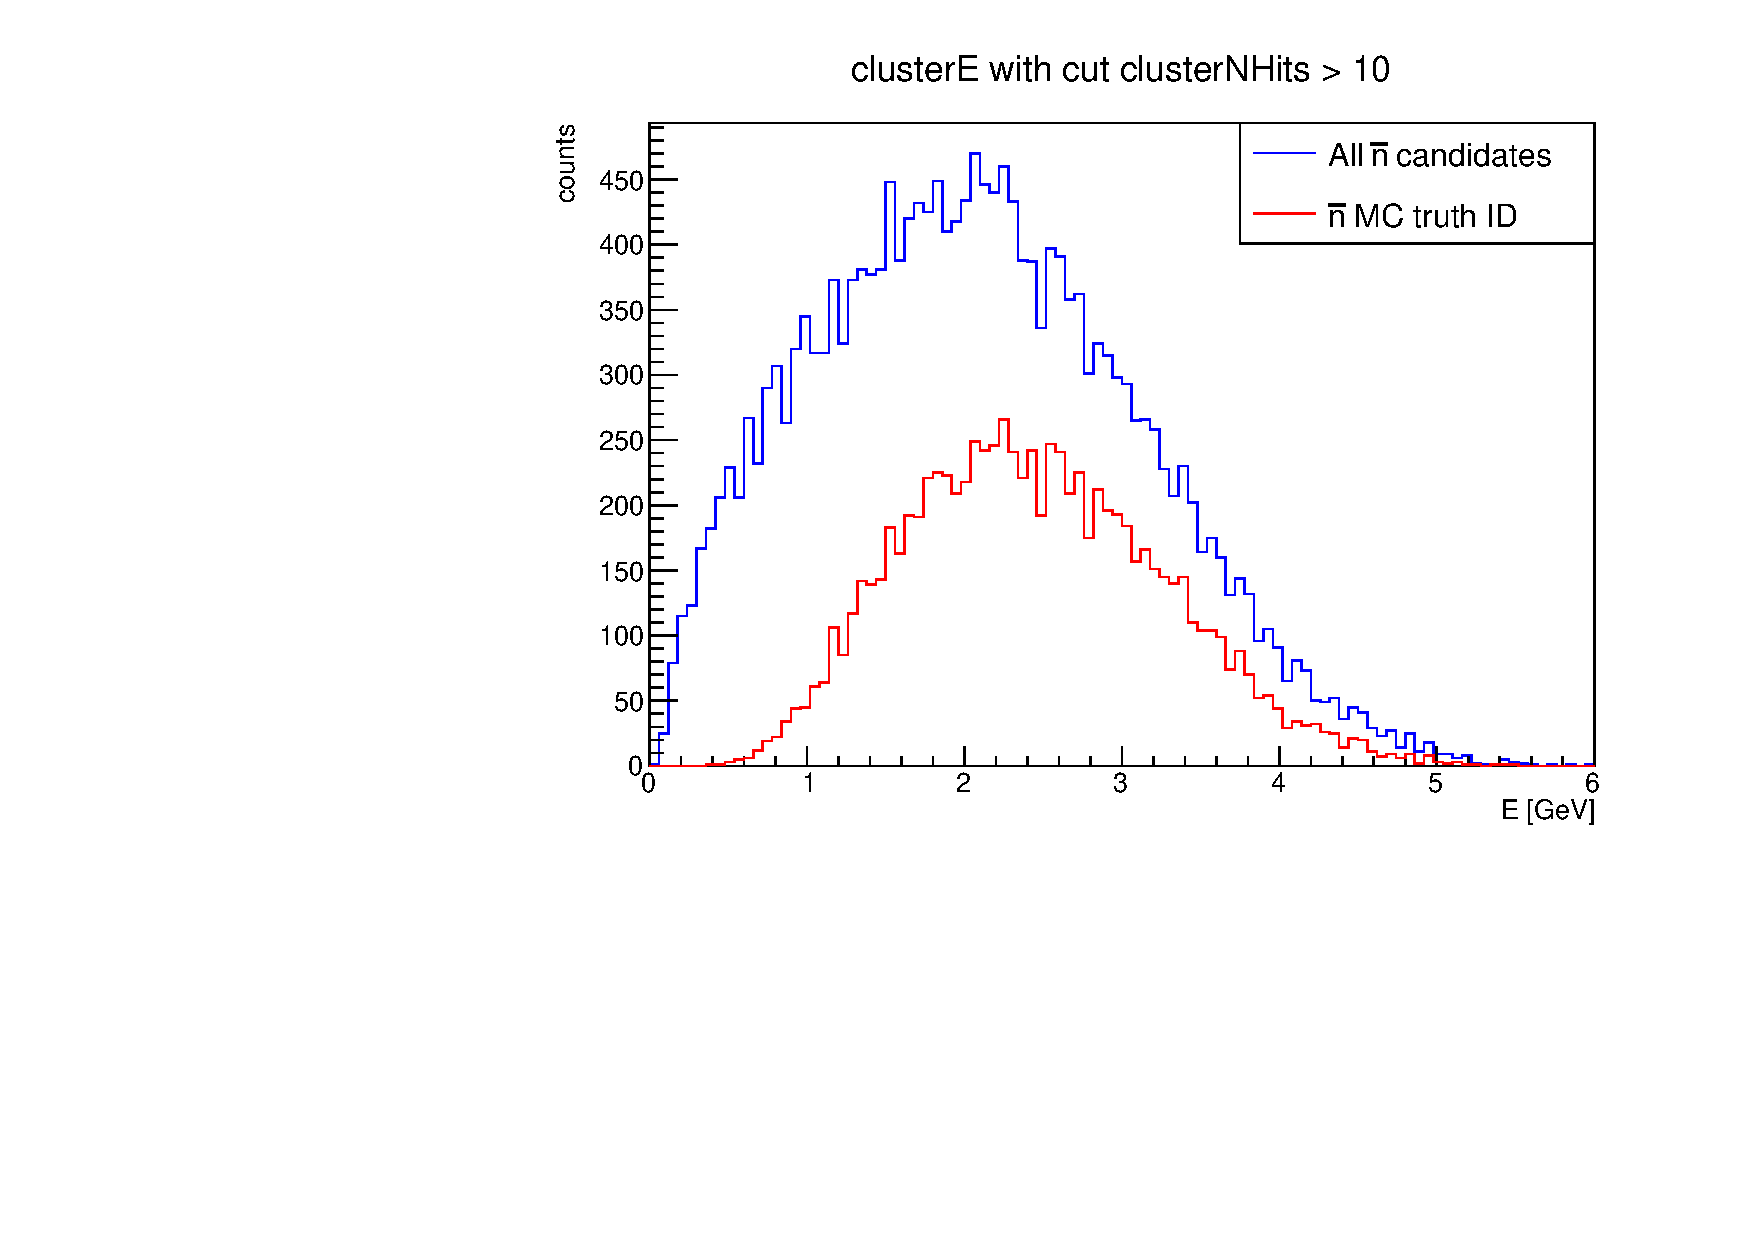
\includegraphics[width=0.49\textwidth]{nbar_MC/images/clusterE_hitscut_nog.pdf}
    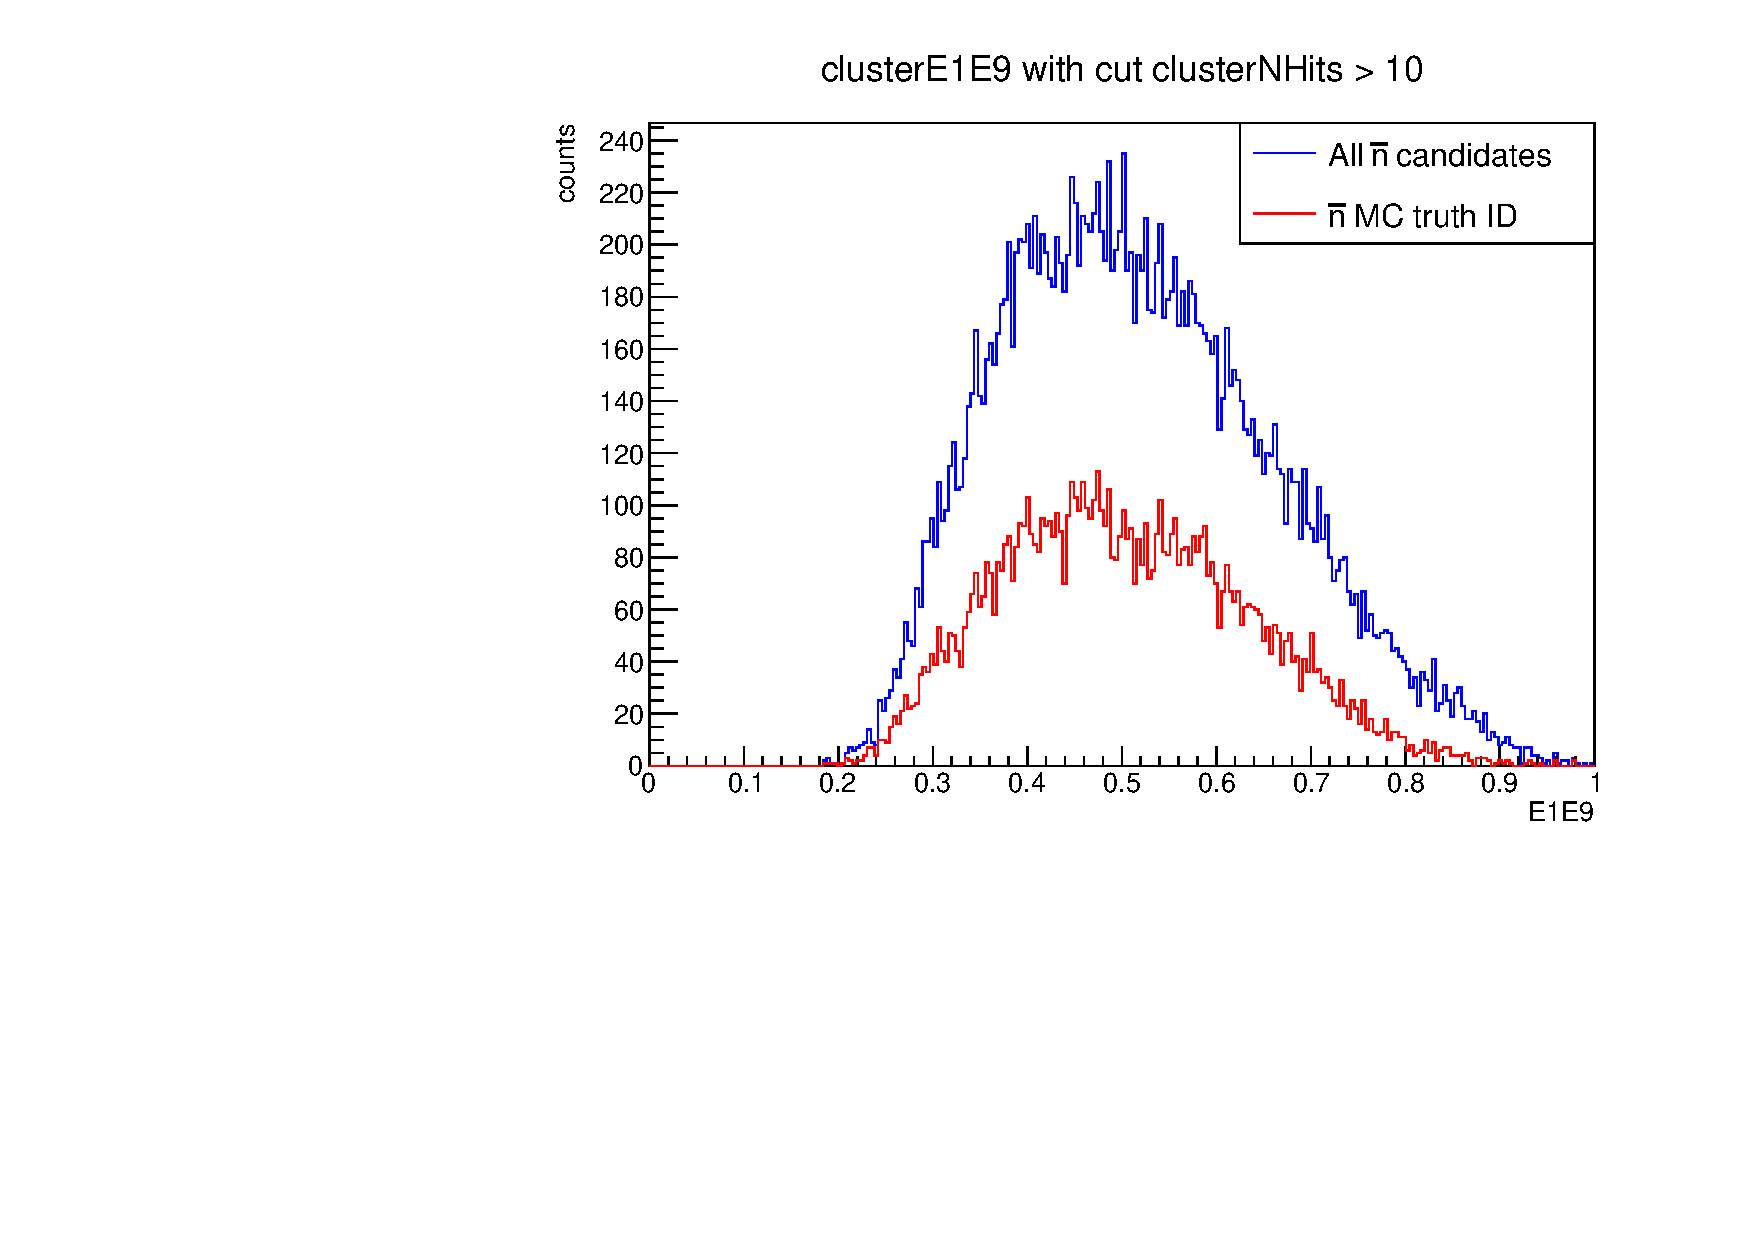
\includegraphics[width=0.49\textwidth]{nbar_MC/images/clusterE1E9_hitscut_nog.pdf}
    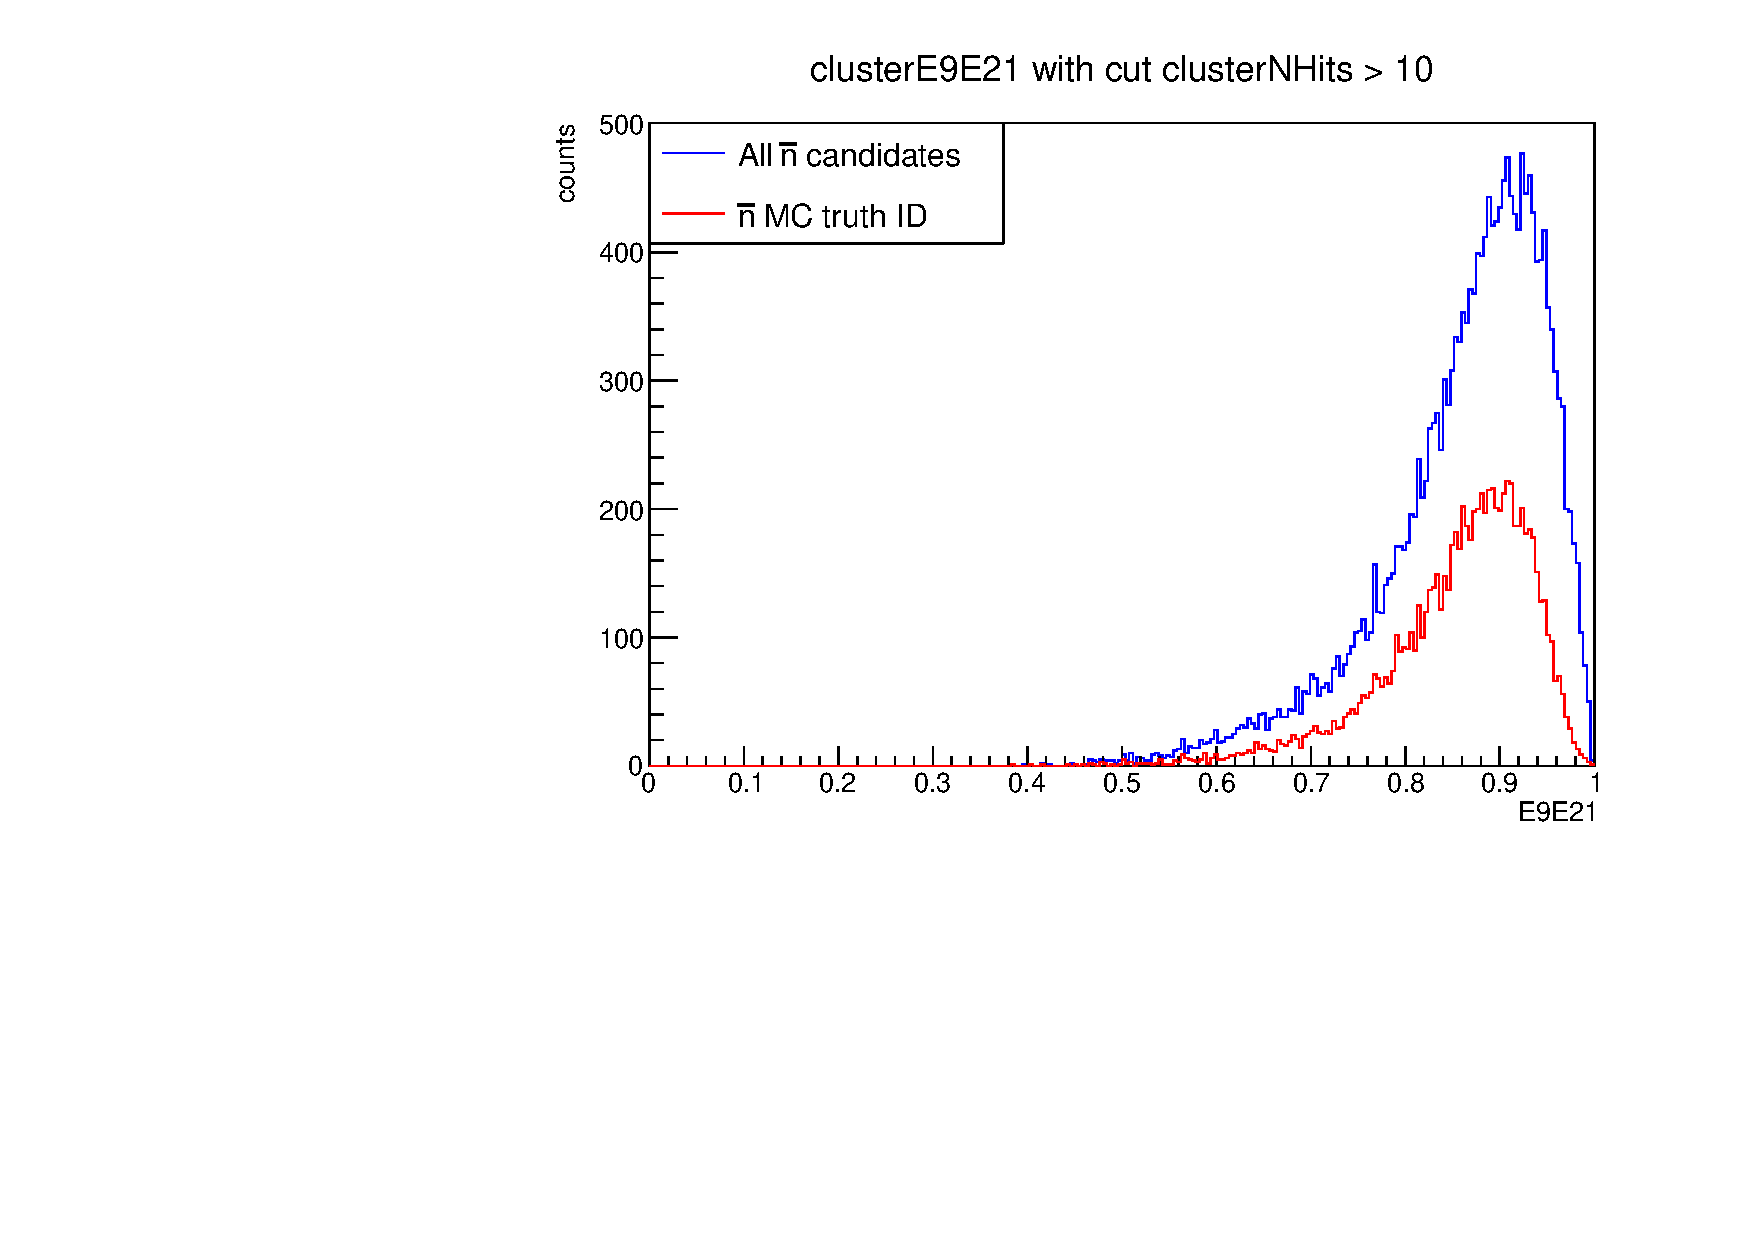
\includegraphics[width=0.49\textwidth]{nbar_MC/images/clusterE9E21_hitscut_nog.pdf}
    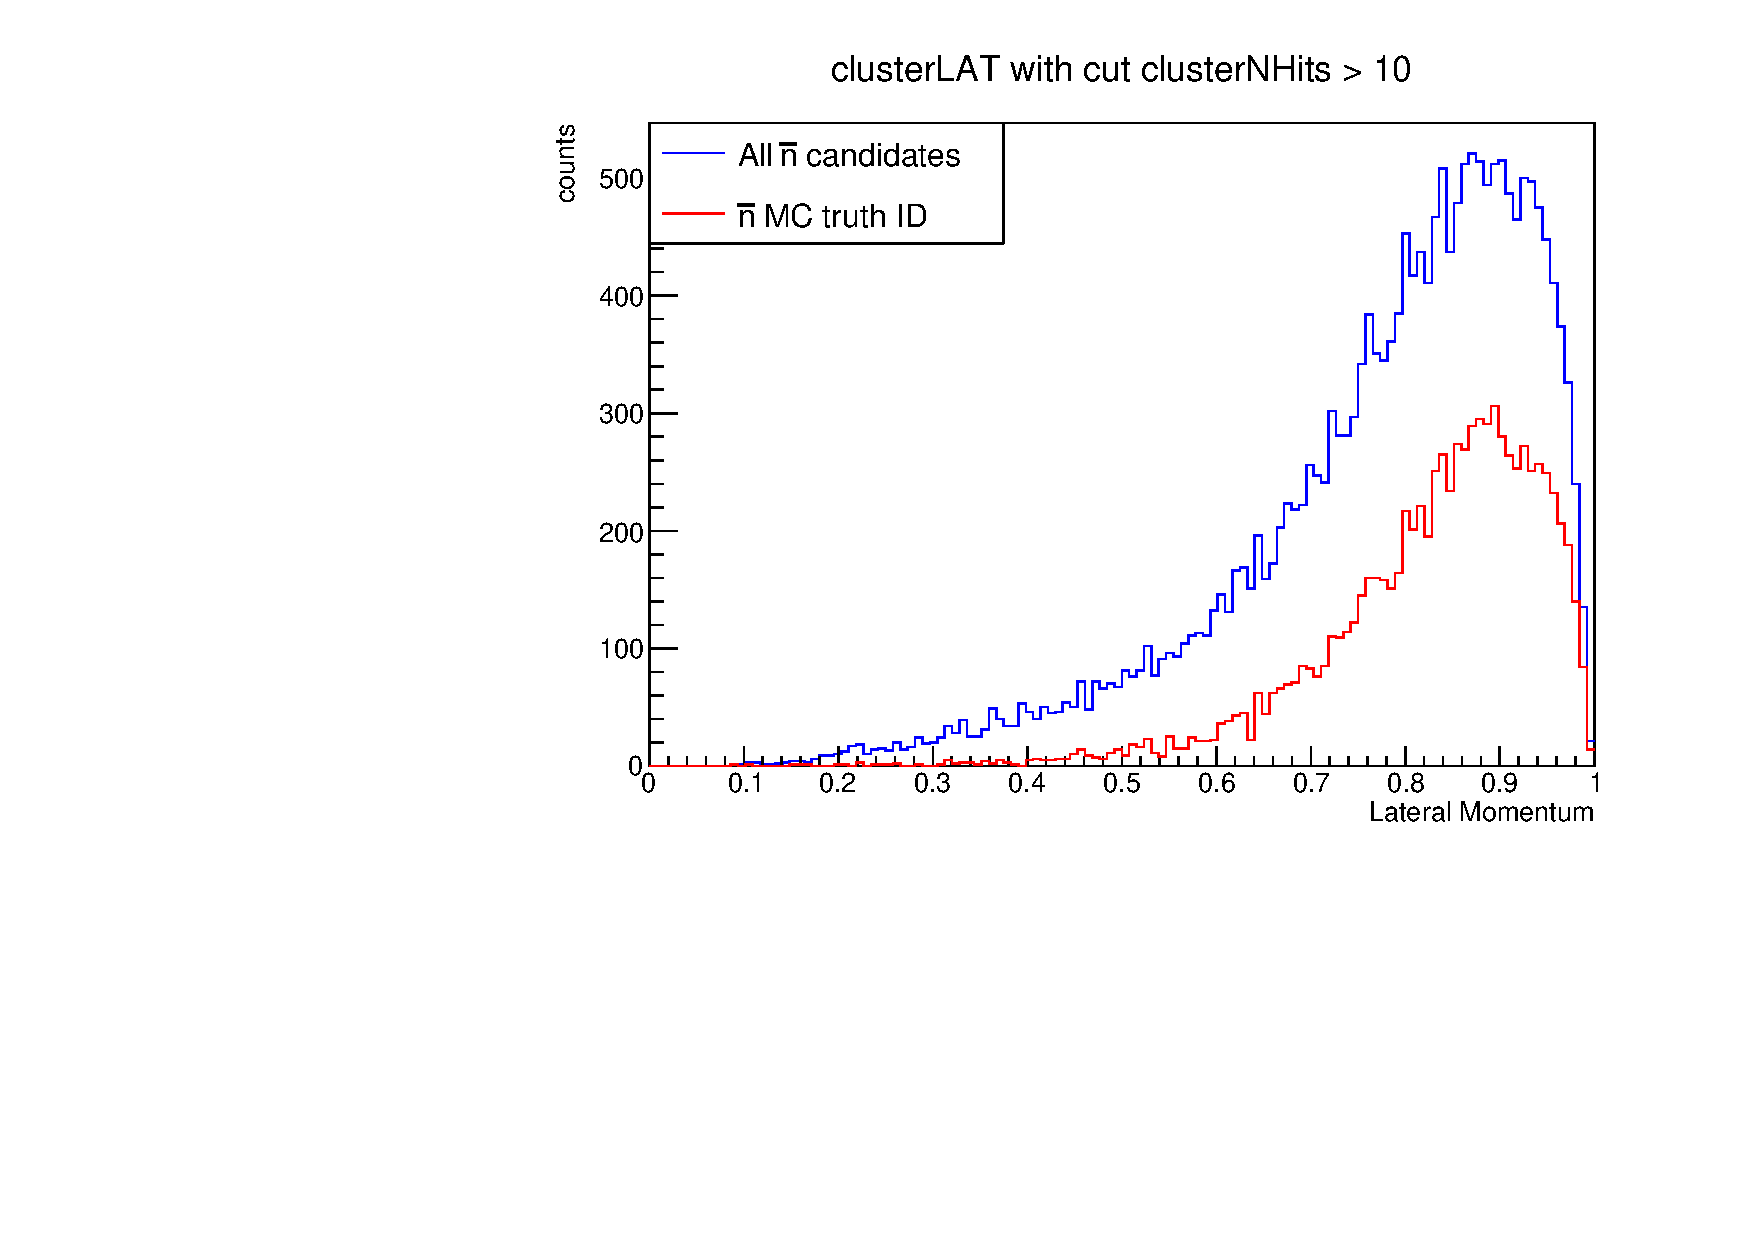
\includegraphics[width=0.49\textwidth]{nbar_MC/images/clusterLAT_hitscut_nog.pdf}
    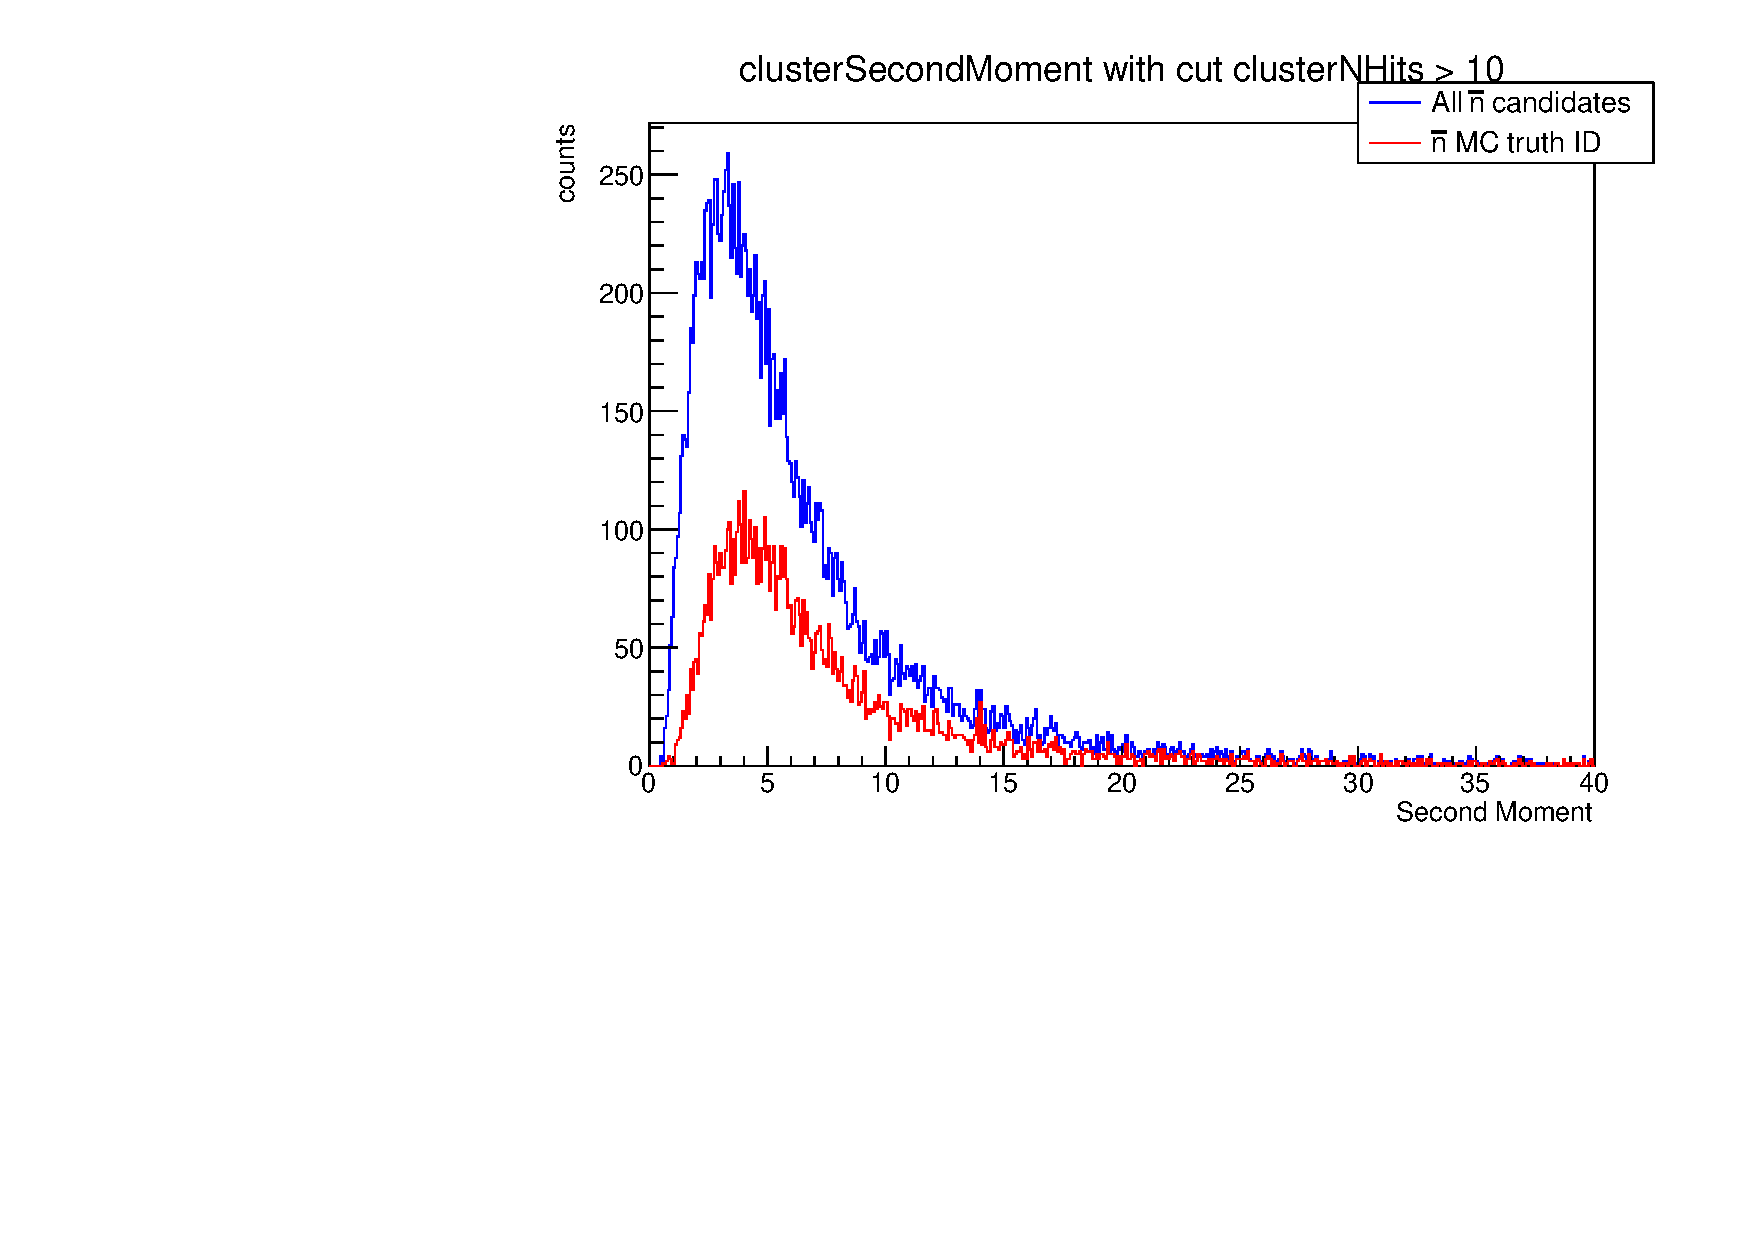
\includegraphics[width=0.49\textwidth]{nbar_MC/images/clusterSecondMoment_hitscut_nog.pdf}
    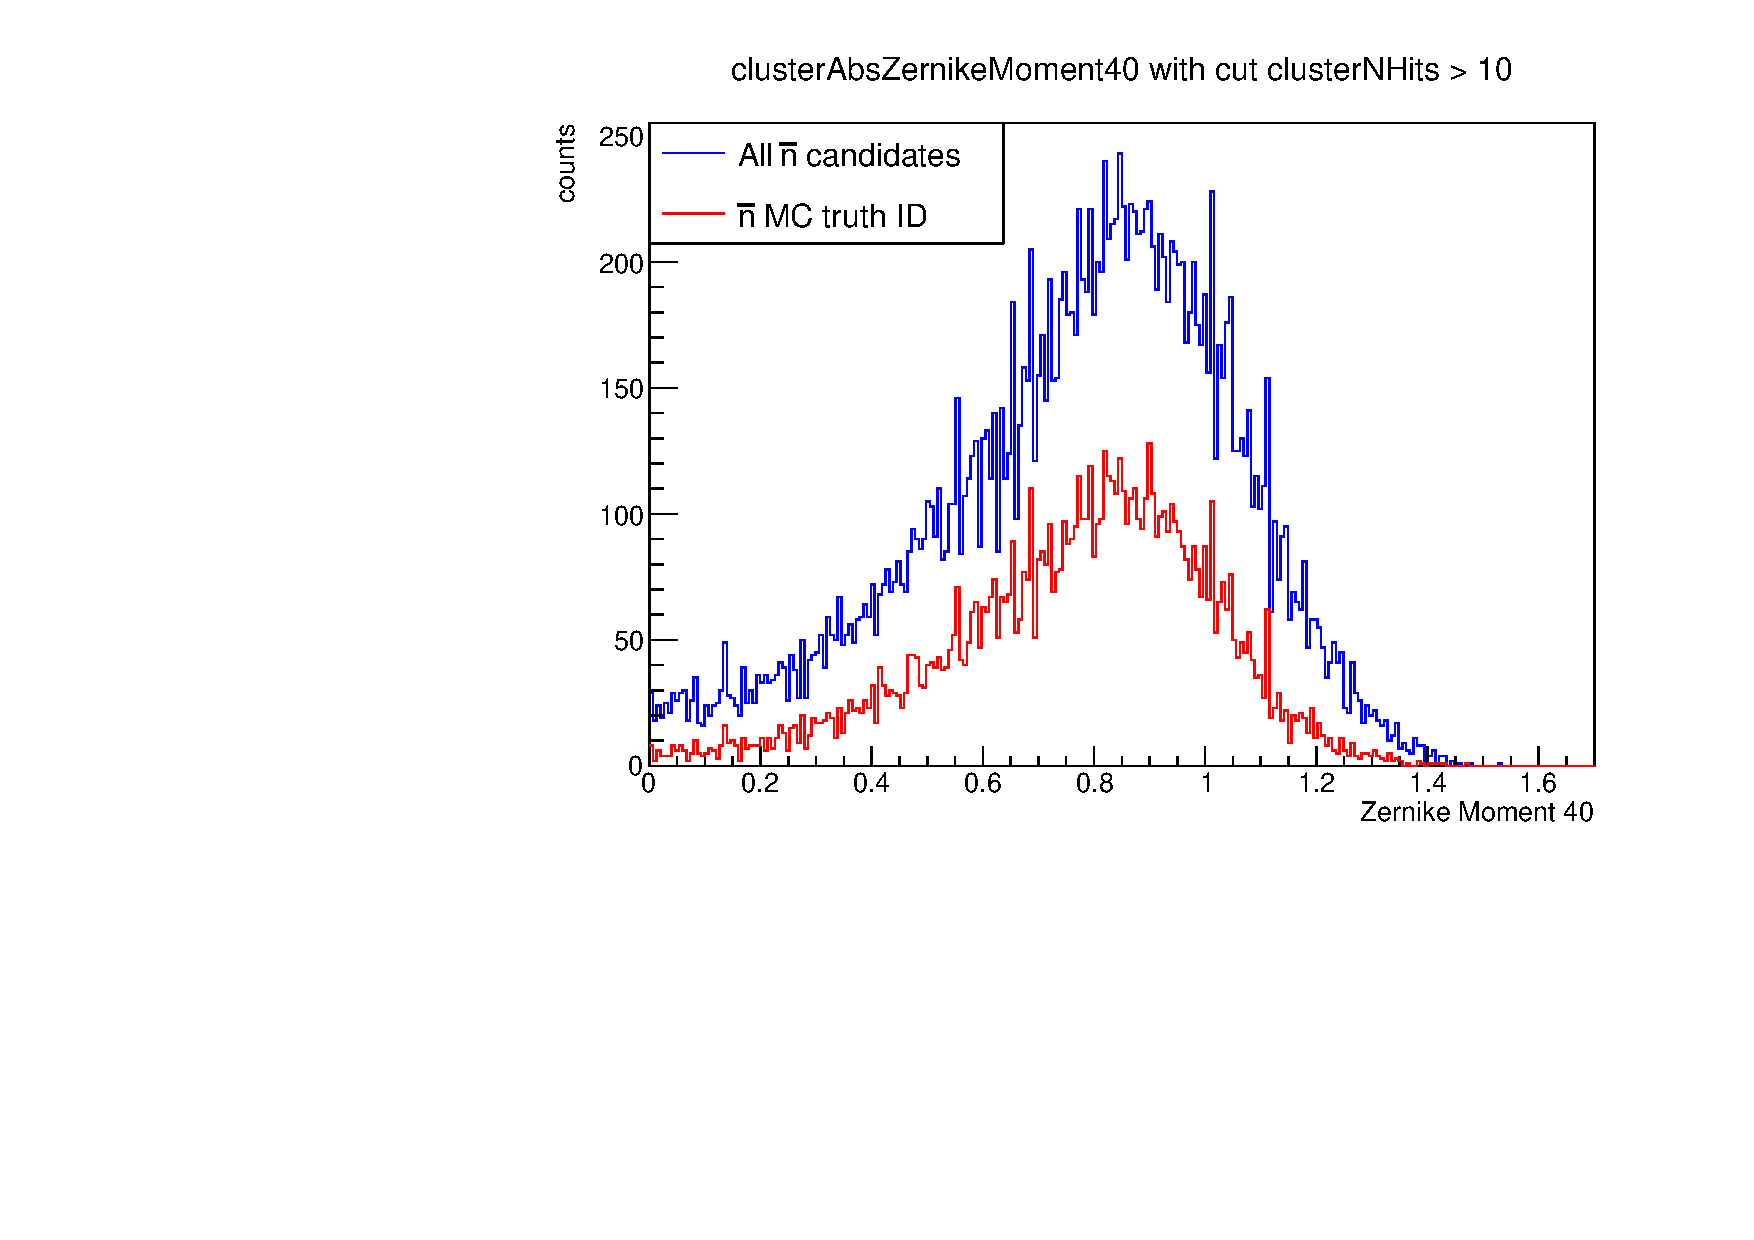
\includegraphics[width=0.49\textwidth]{nbar_MC/images/clusterAbsZernikeMoment40_hitscut_nog.pdf}
    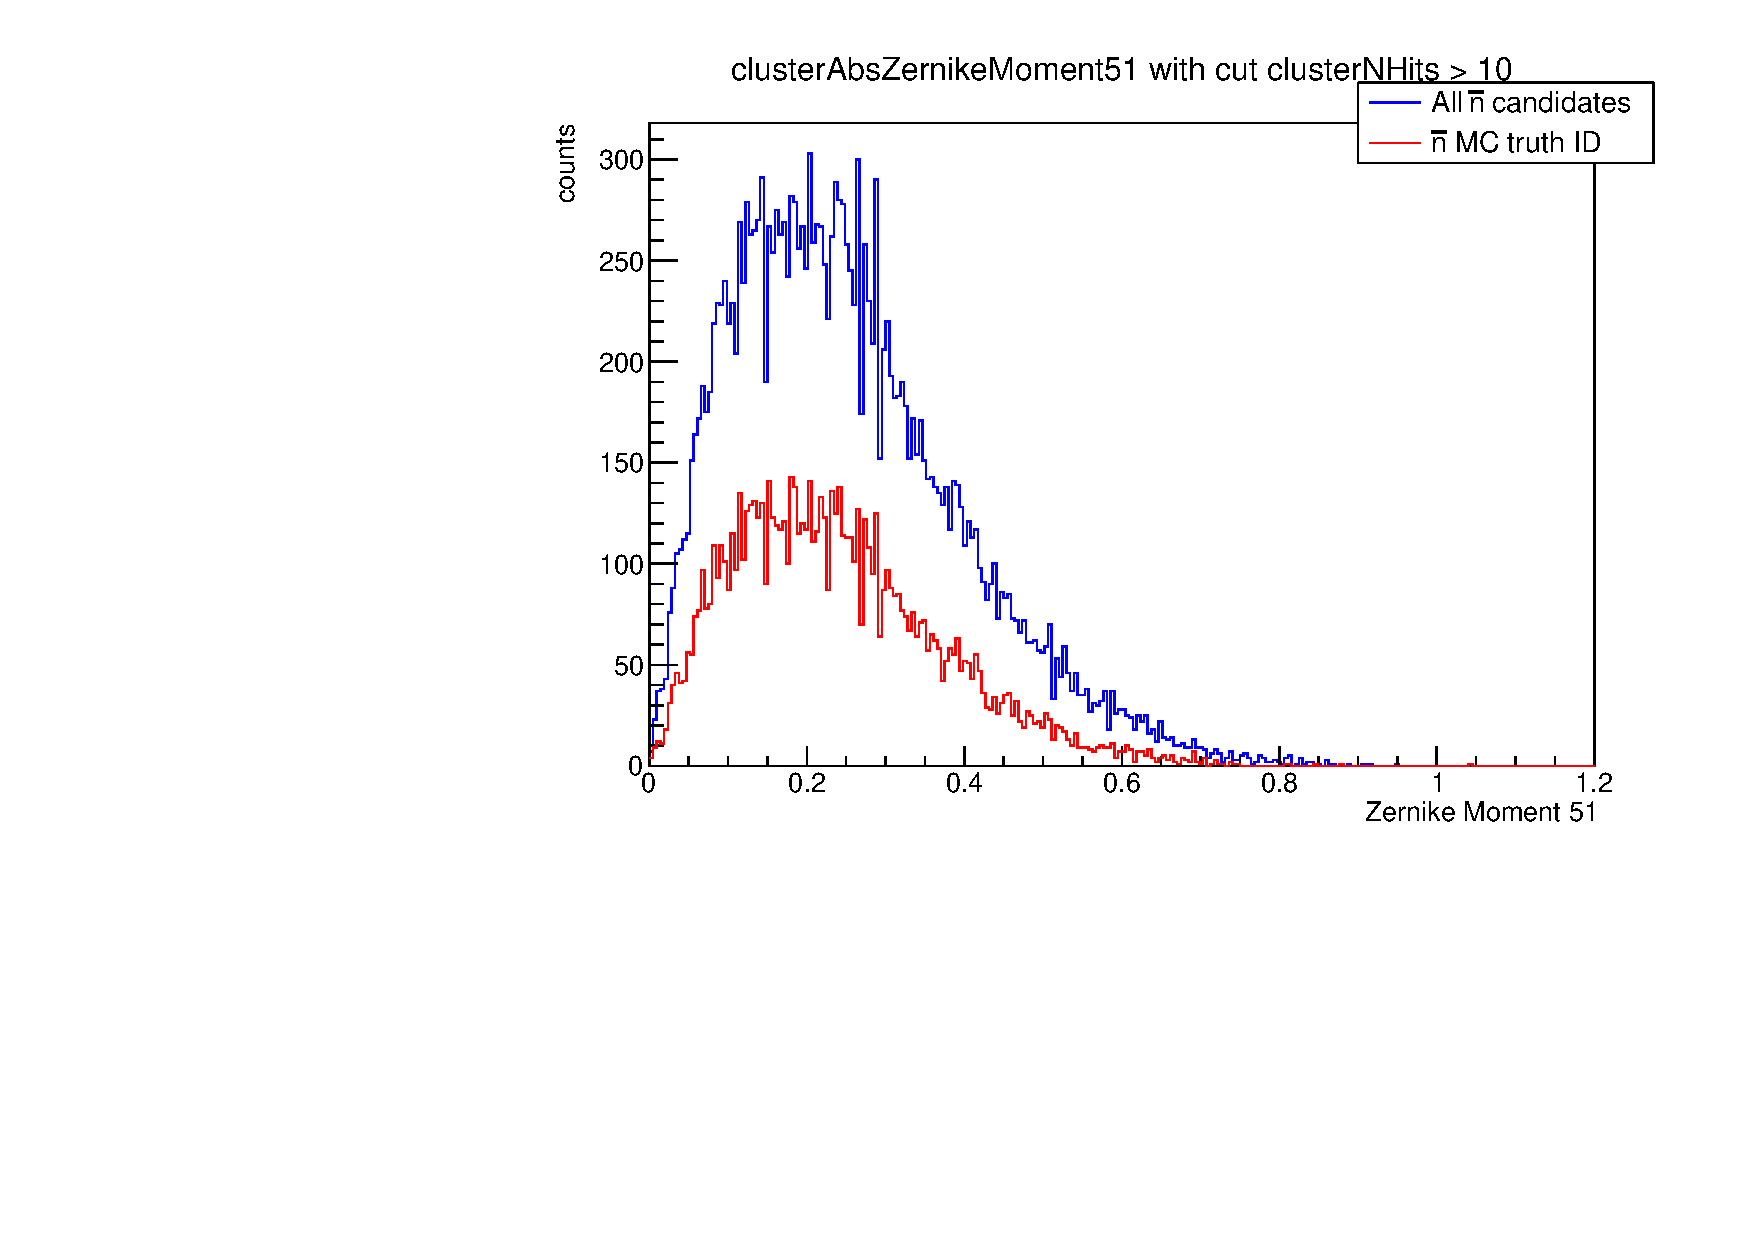
\includegraphics[width=0.49\textwidth]{nbar_MC/images/clusterAbsZernikeMoment51_hitscut_nog.pdf}
    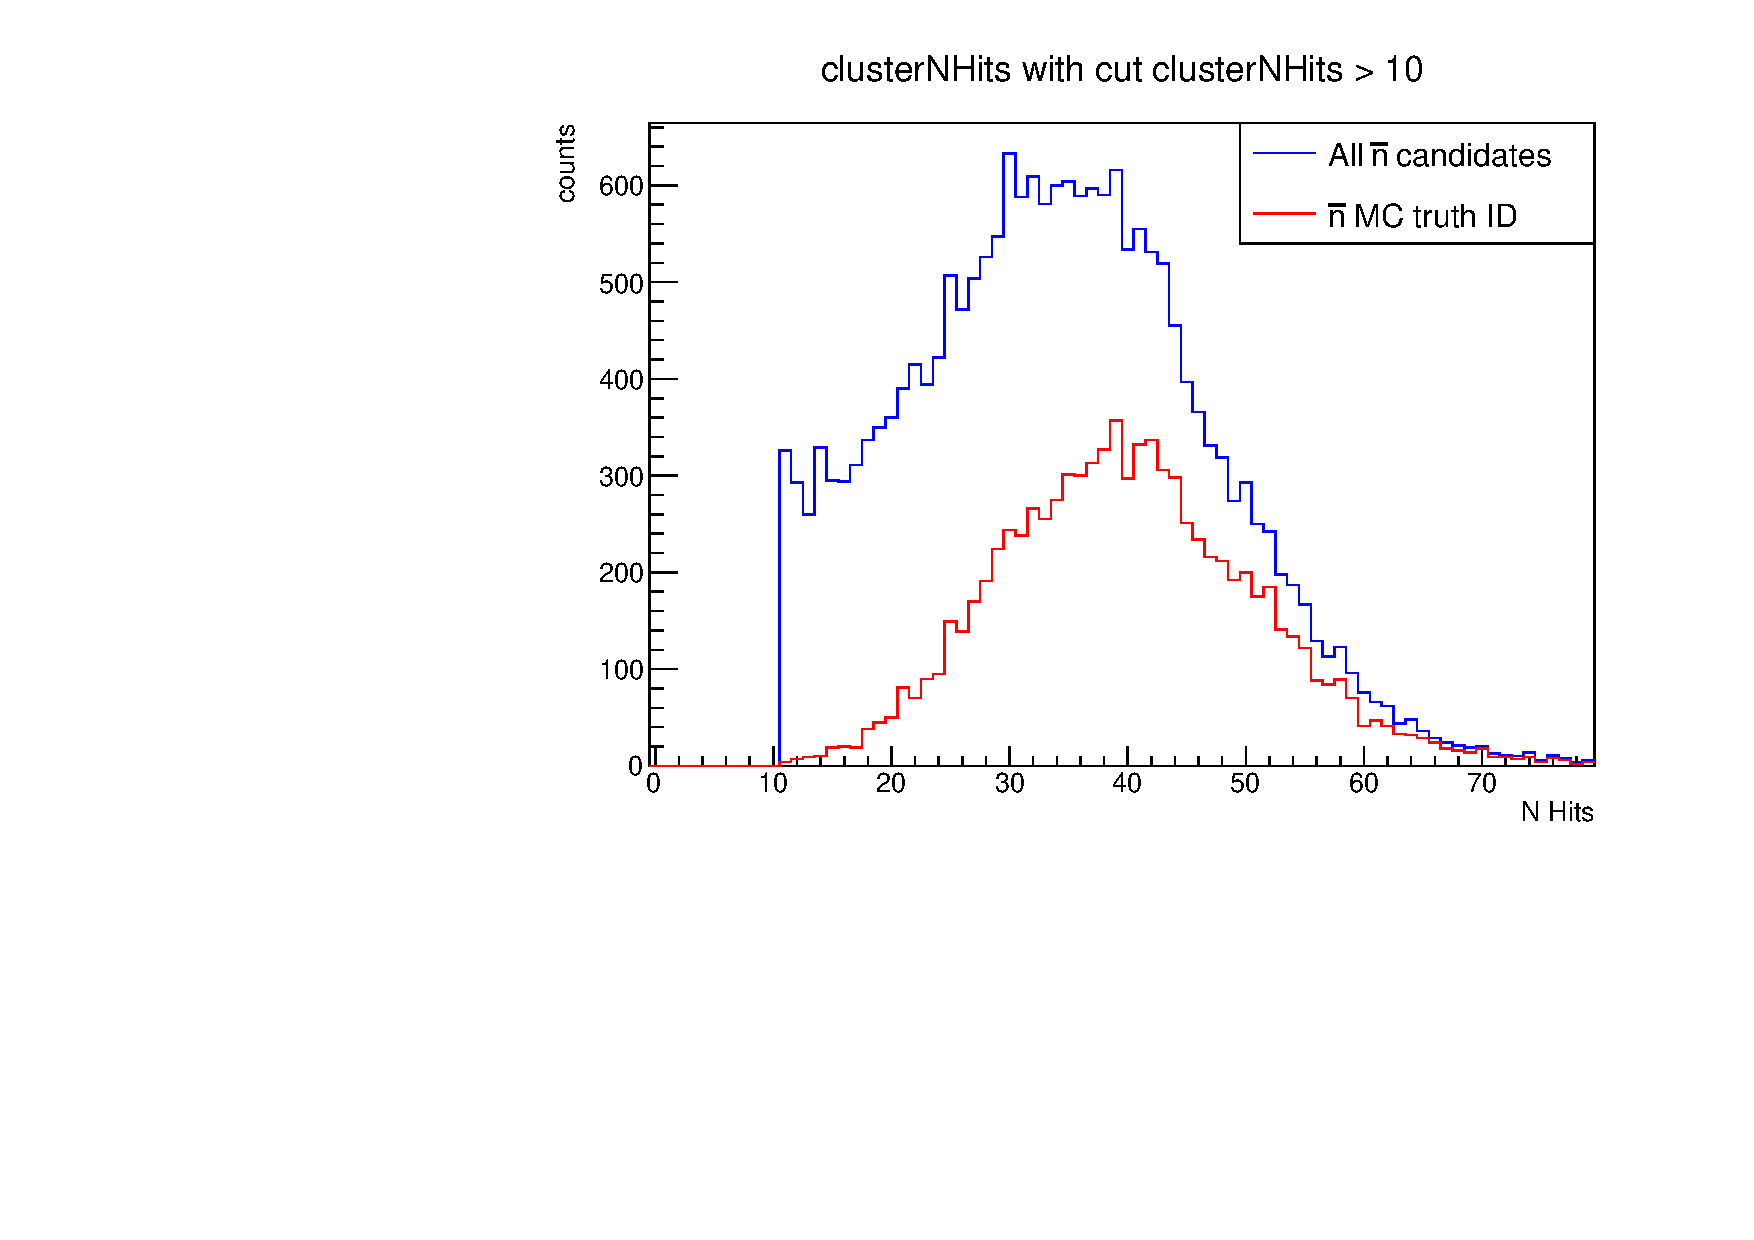
\includegraphics[width=0.49\textwidth]{nbar_MC/images/clusterNHits_hitscut_nog.pdf}
   
     \caption{Comparison of reconstructed cluster variables for all $\bar{n}$ candidates versus those associated with $\bar{n}$ particles by Monte Carlo truth Monte Carlo PDG = -2112 (NO ISR case). Cut $clusterNHits > 10$ is performed}
     
     \label{fig:cluster_NOISR_NHits}

\end{figure}

\newpage

\subsubsection{Cluster variables in different ECL regions}
As described in Chapter 3, the Belle II detector is divided into barrel and forward/backward end-cap regions. It would be interesting to study the reconstructed cluster variables in each ECL region separately. Since the ISR and NO ISR cases exhibit analogous shower shapes, only the latter is discussed here.
$\\$
The region hit distribution is shown below:
 \begin{figure}[H]
    \centering
    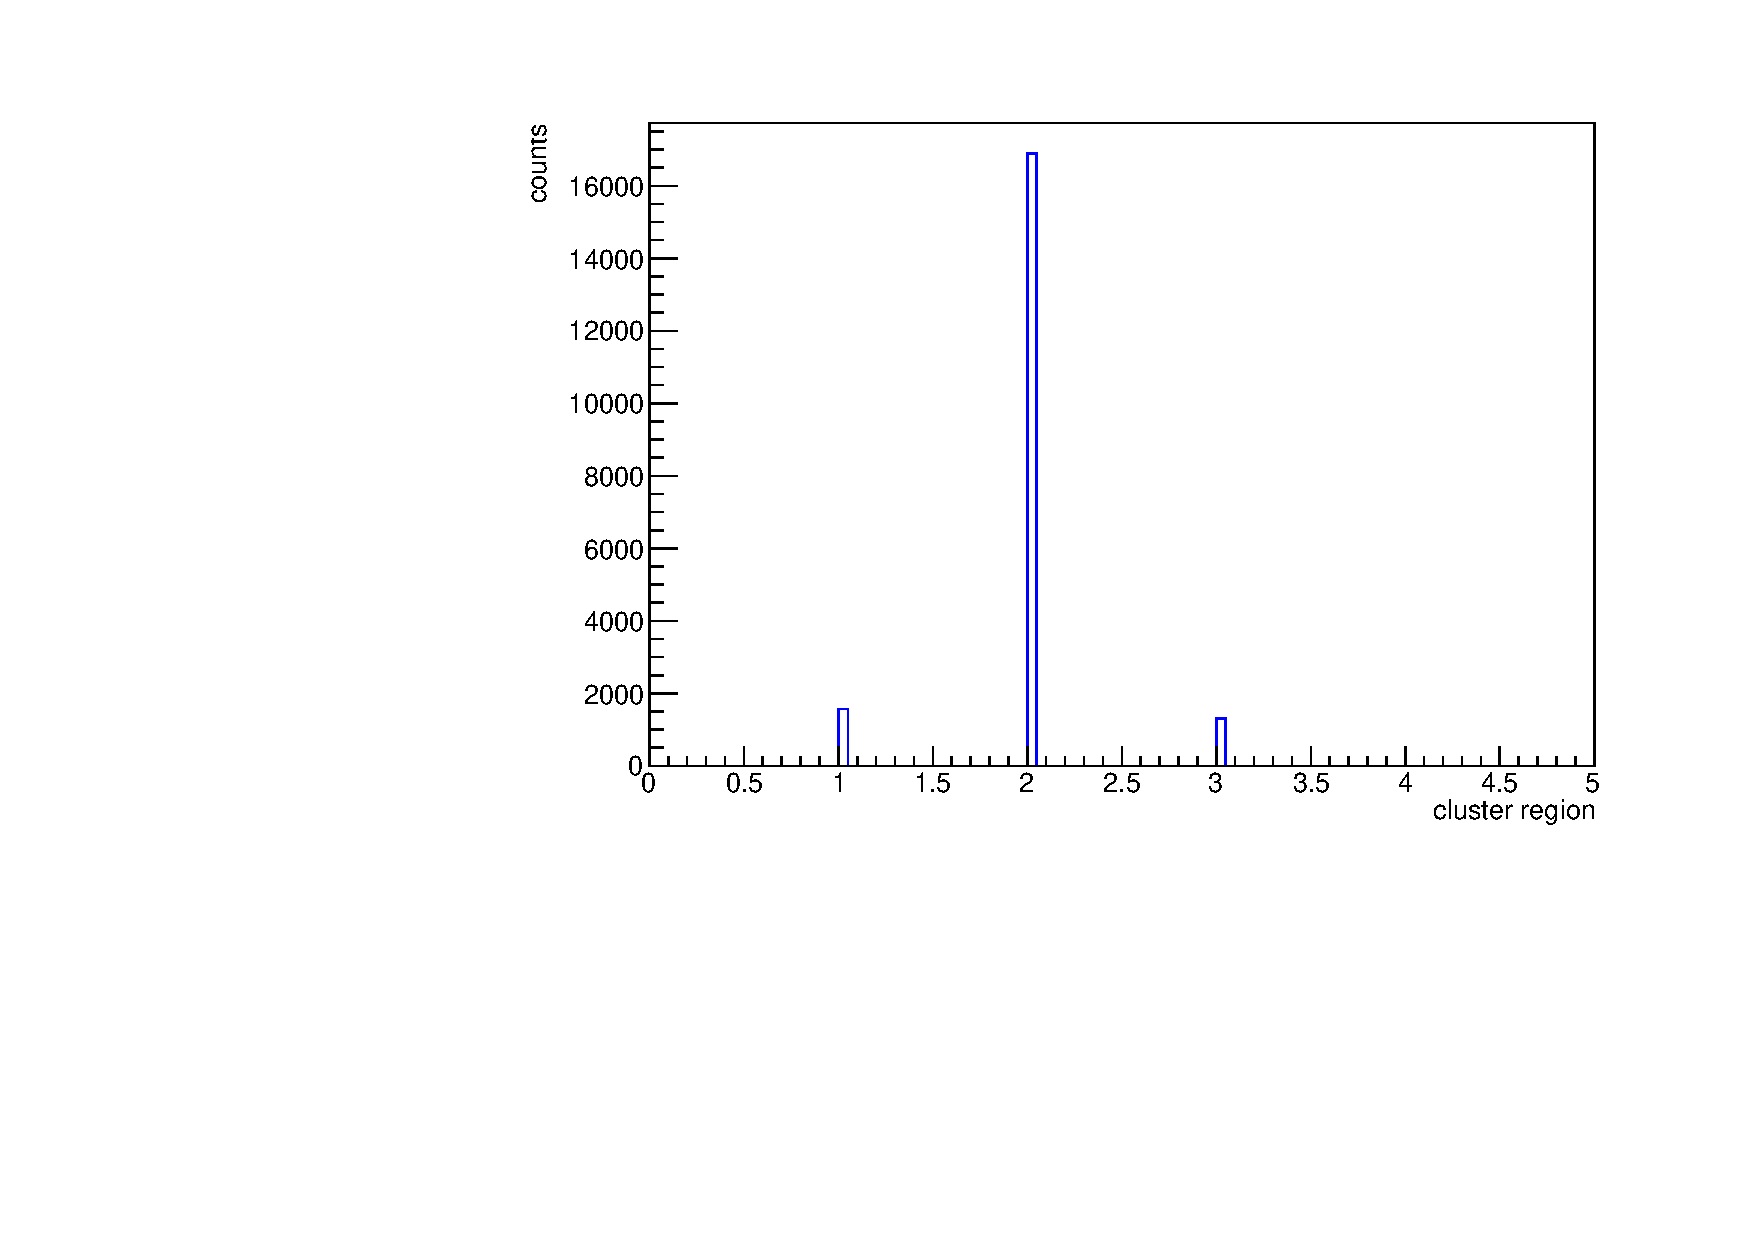
\includegraphics[width=0.80\textwidth]{nbar_MC/images/cluster_region.pdf}

     \caption{Different ECL regions contribution in neutral cluster associated to $\bar{n}$ candidates, where 1 is the forward region, 2 is the barrel region and 3 is the backward region. As expected, the barrel region is the most involved}

\end{figure}

As observed in Fig.~\ref{fig:cluster_region}, the cluster variable associated to all the reconstructed  $\bar{n}$ shapes are consistent across all ECL regions. 
$\\$
However a slight difference can be noted for cluster energy and number of hits variables. In fact, these two exhibit a shift toward lower values in the forward region, reflecting the Lorentz boost of the center-of-mass. In any case, the barrel region contains the majority of ECL clusters, as expected.

\newpage
The obtained cluster variables in NO ISR case are shown below:
 \begin{figure}[H]
    \centering
    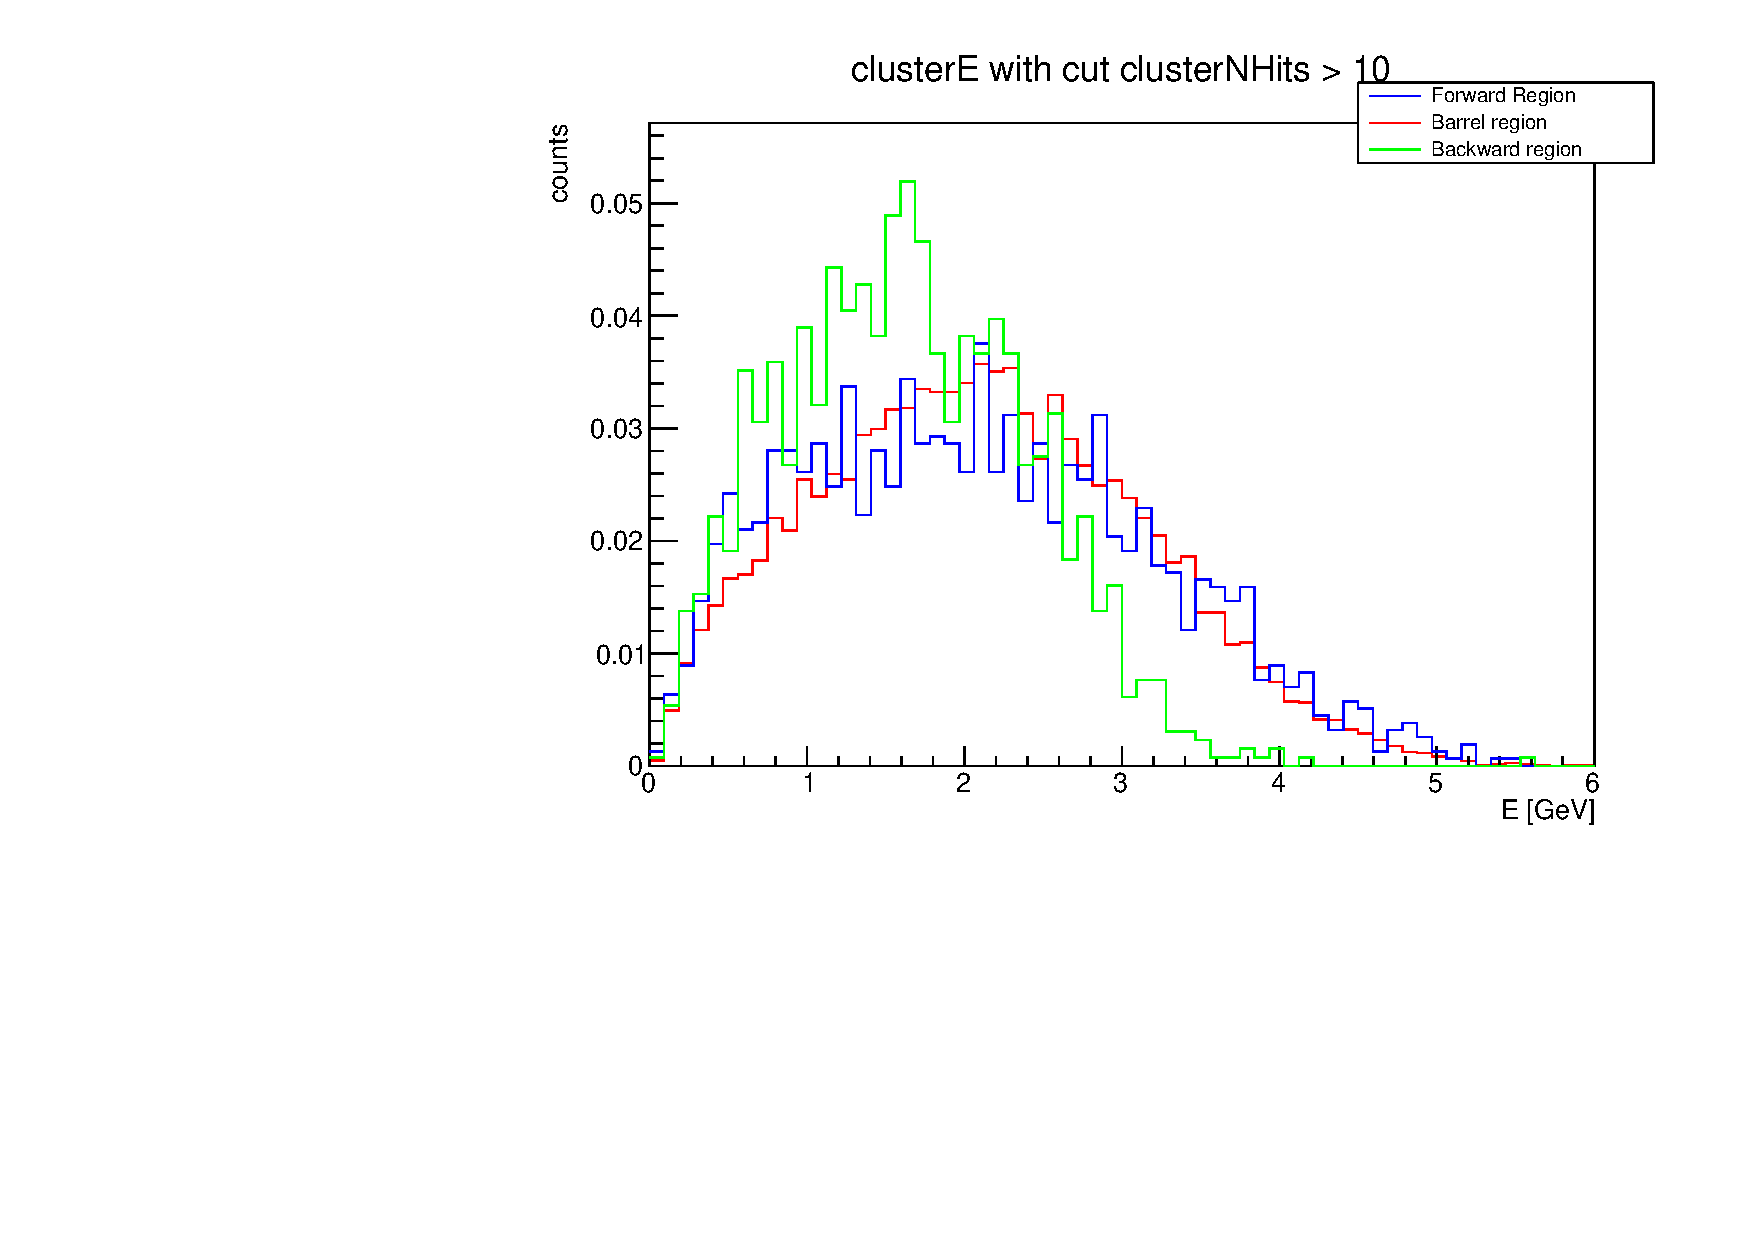
\includegraphics[width=0.49\textwidth]{nbar_MC/images/clusterE_nog_region.pdf}
    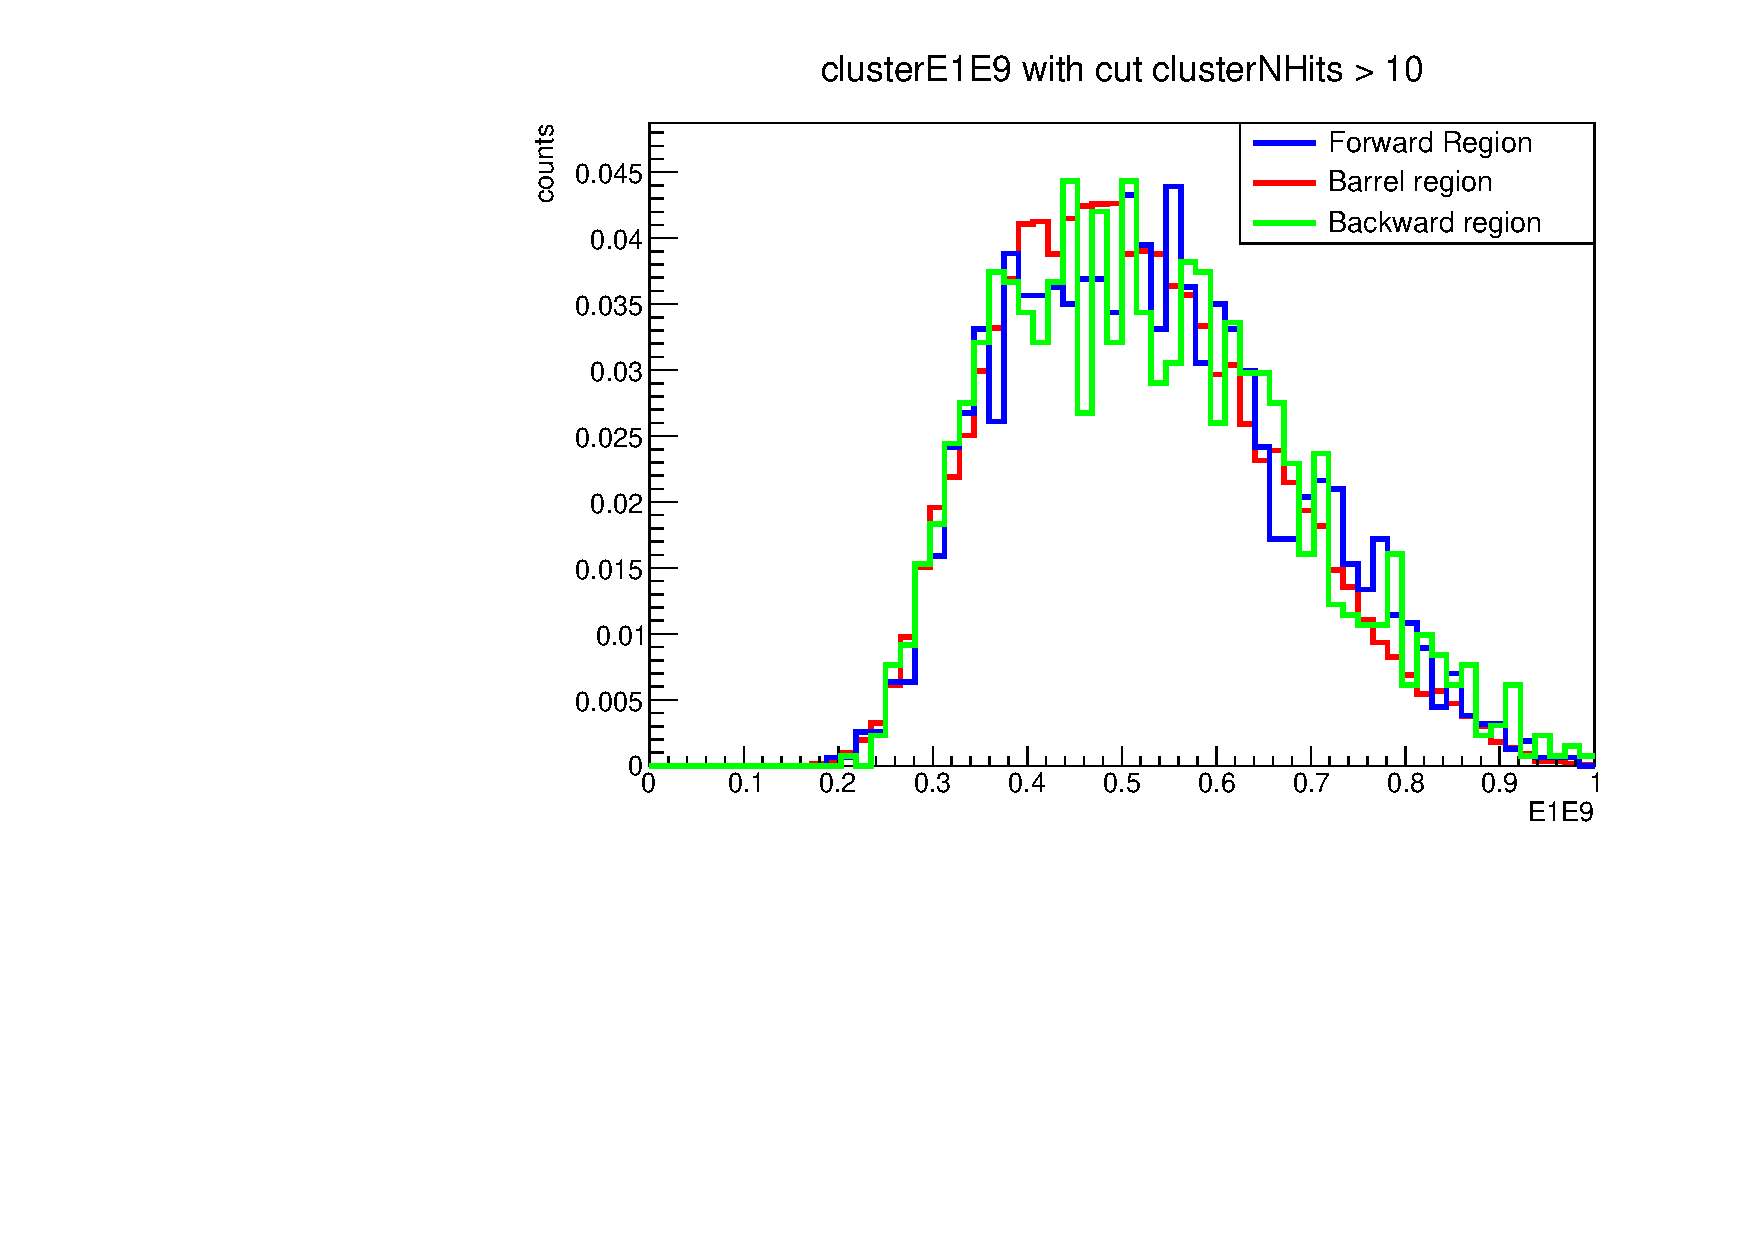
\includegraphics[width=0.49\textwidth]{nbar_MC/images/clusterE1E9_nog_region.pdf}
    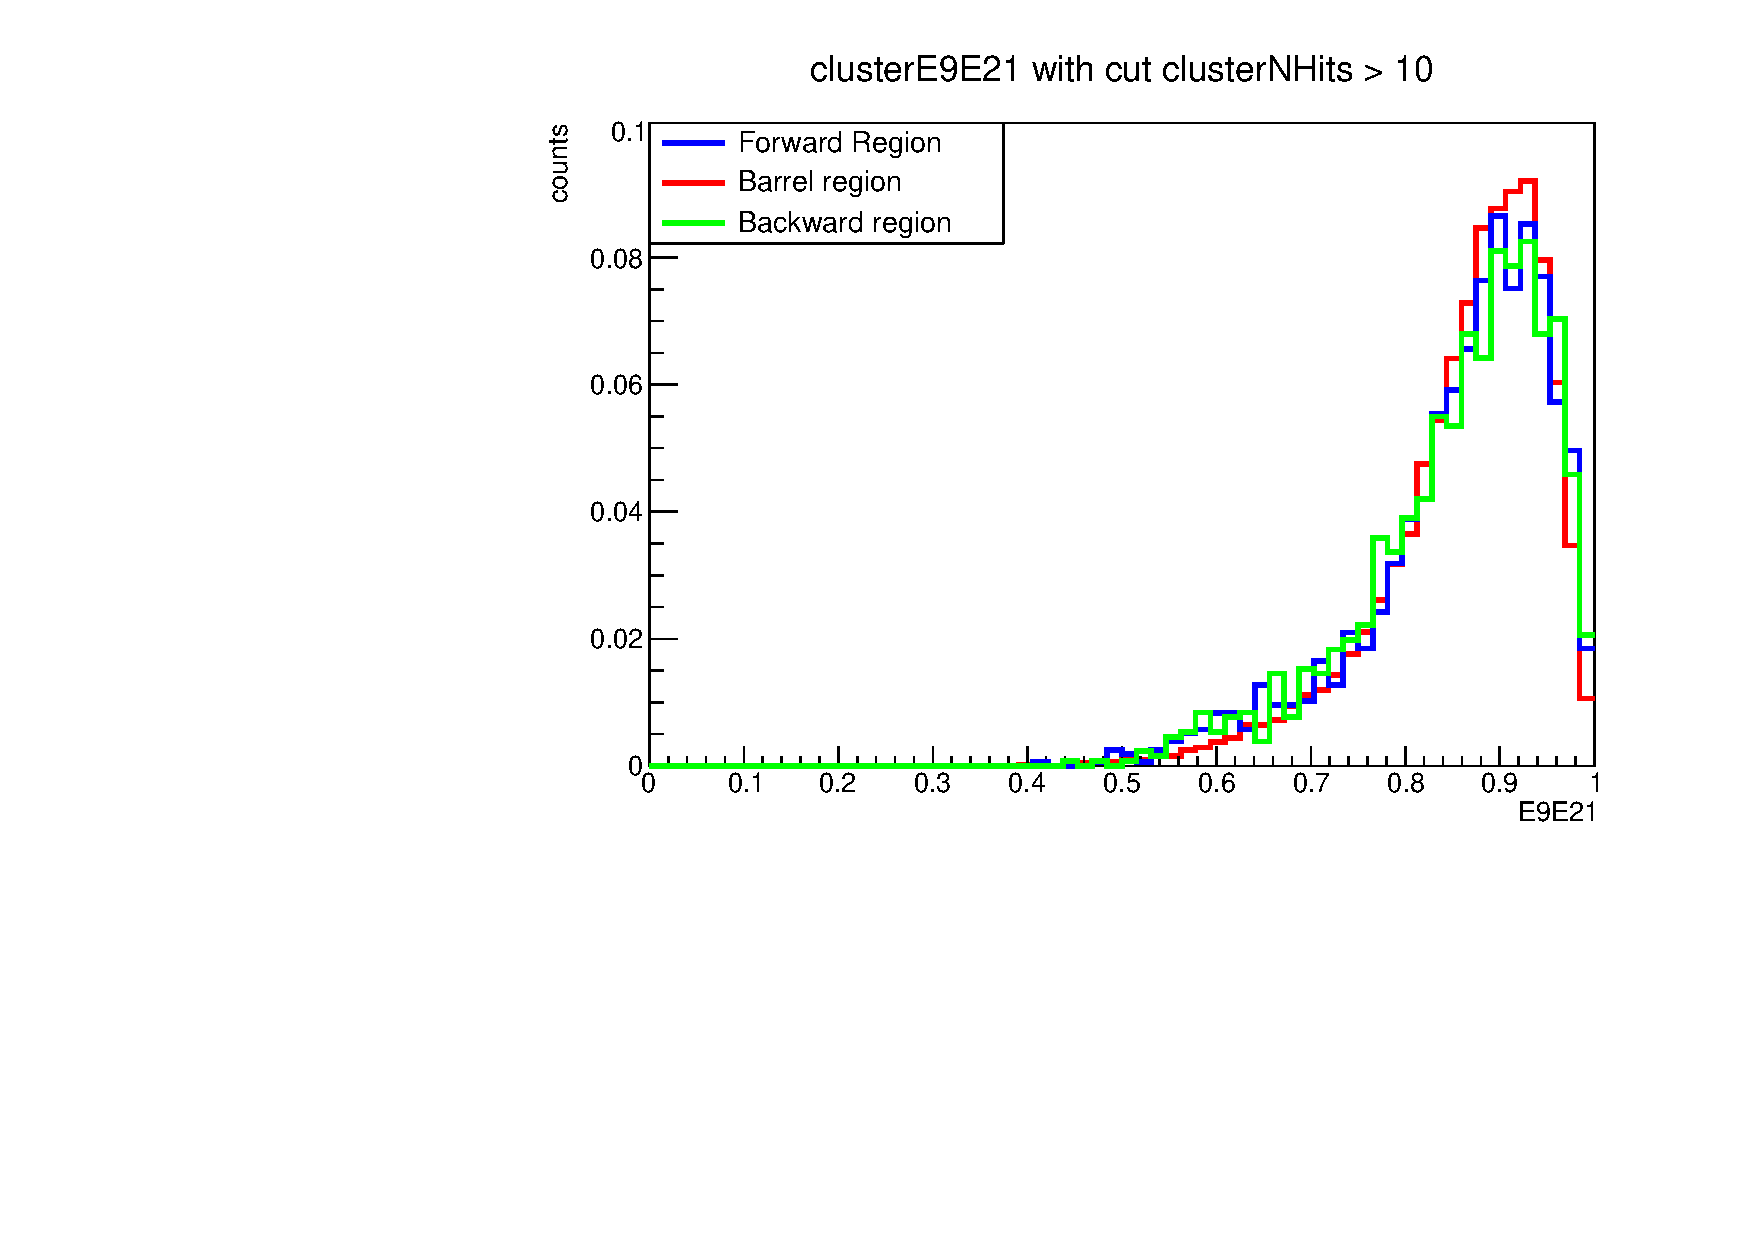
\includegraphics[width=0.49\textwidth]{nbar_MC/images/clusterE9E21_nog_region.pdf}
    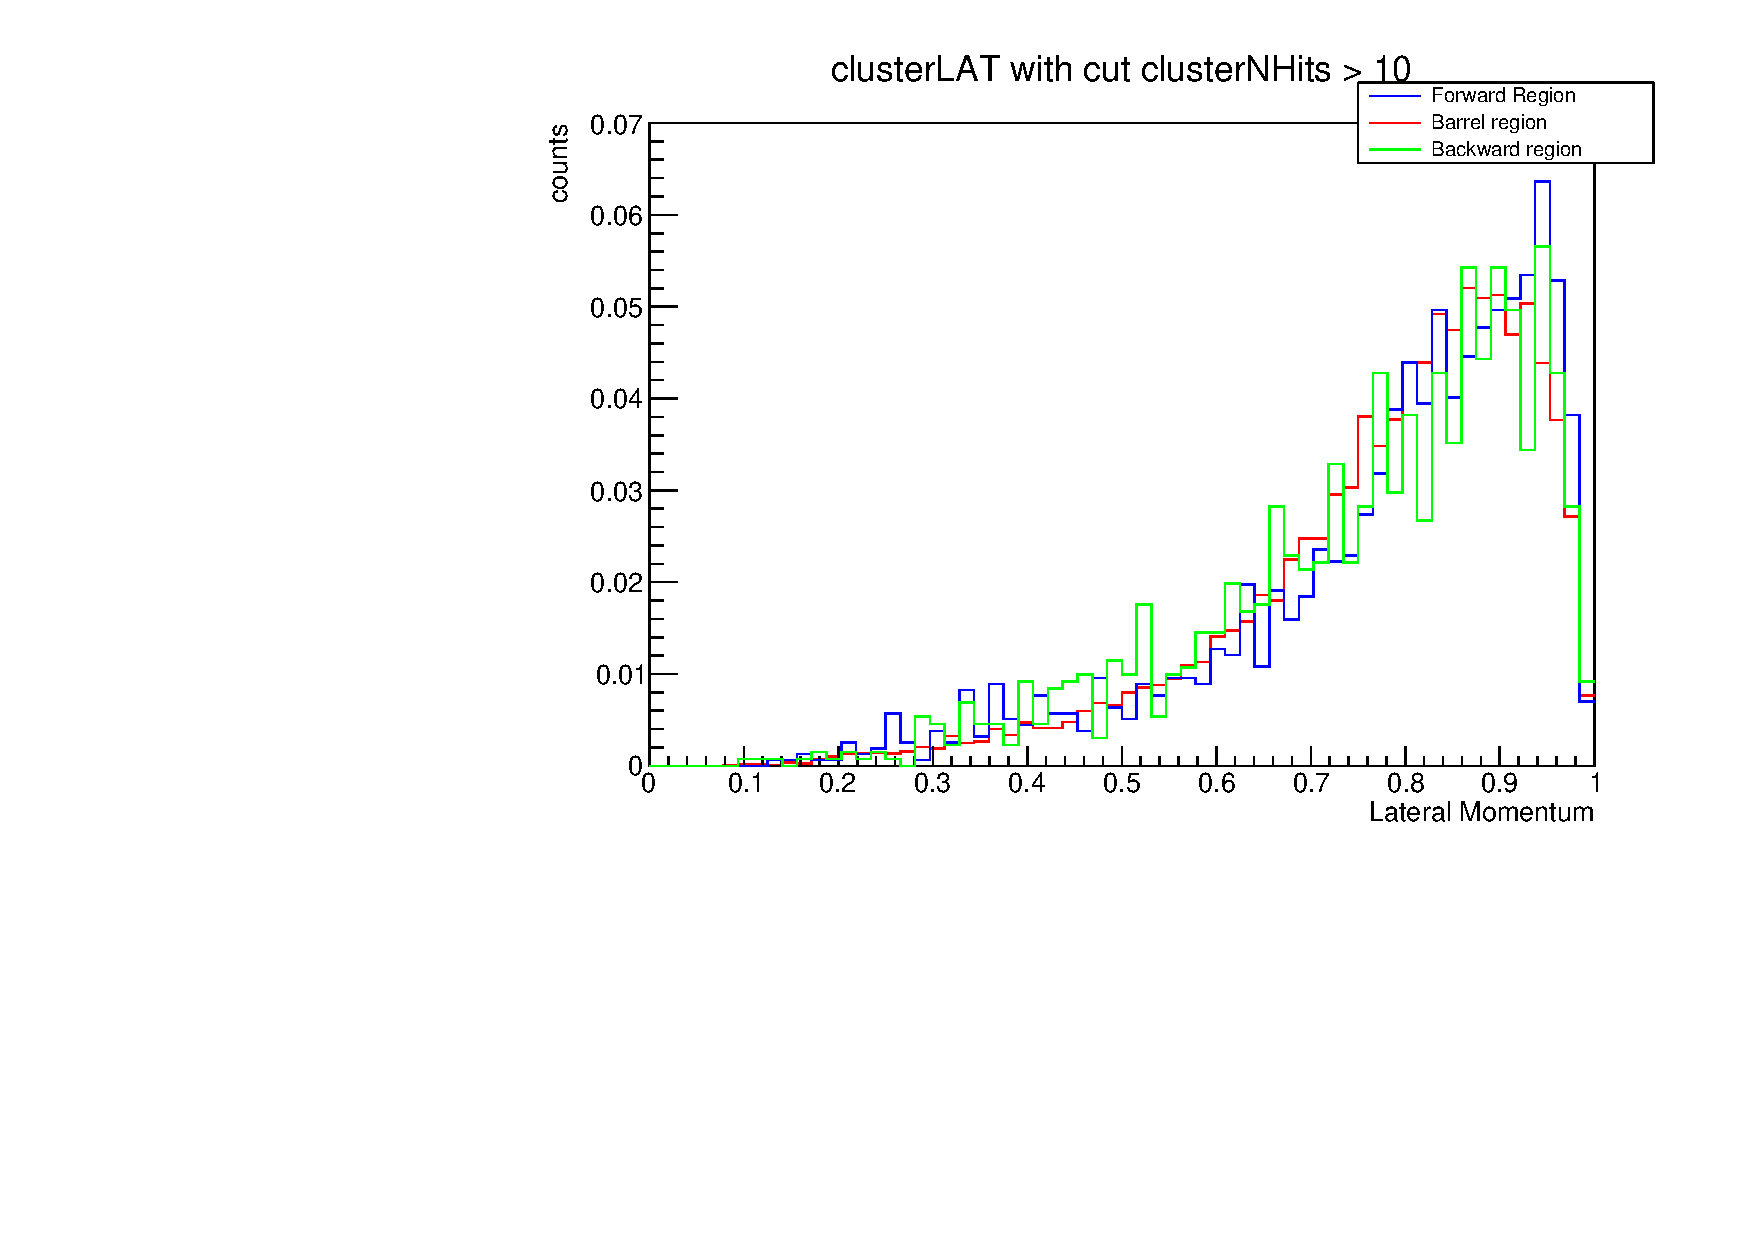
\includegraphics[width=0.49\textwidth]{nbar_MC/images/clusterLAT_nog_region.pdf}
    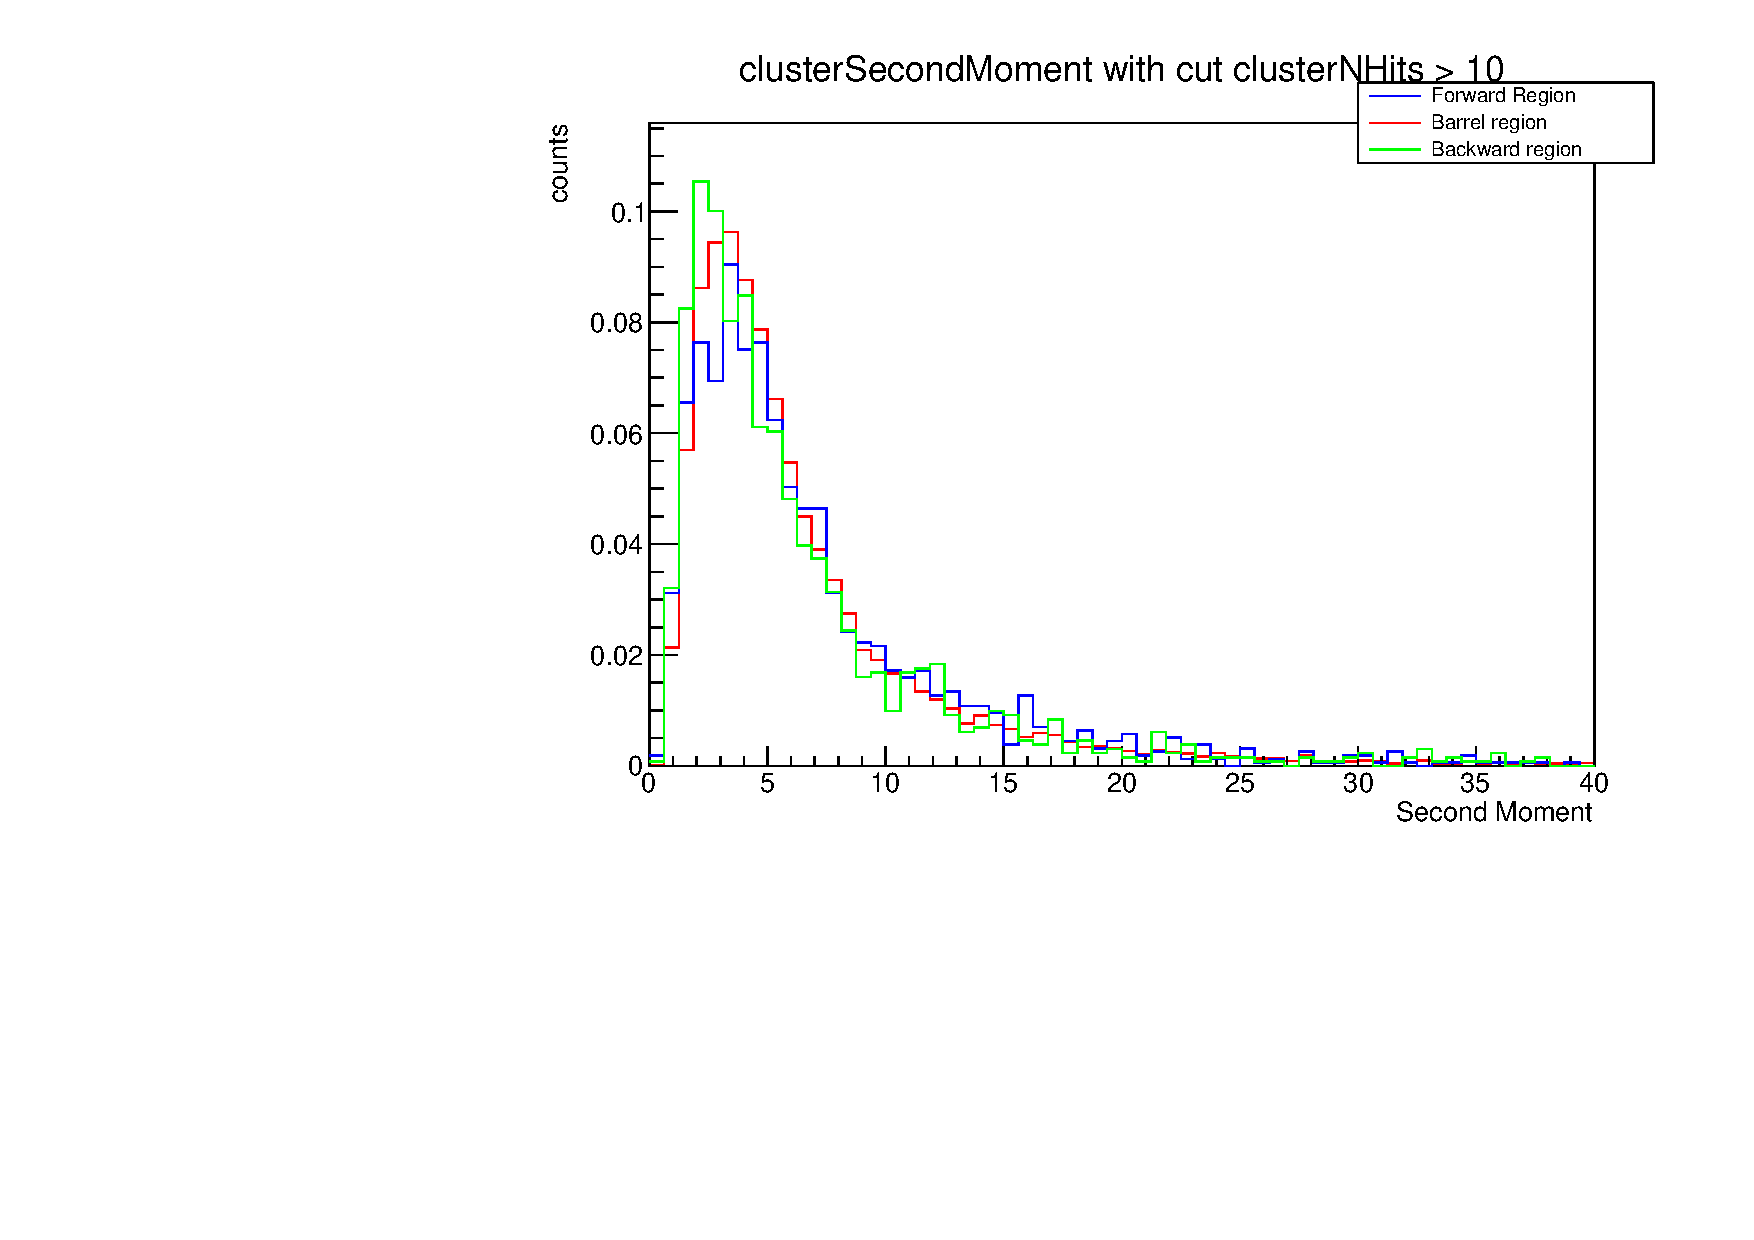
\includegraphics[width=0.49\textwidth]{nbar_MC/images/clusterSecondMoment_nog_region.pdf}
    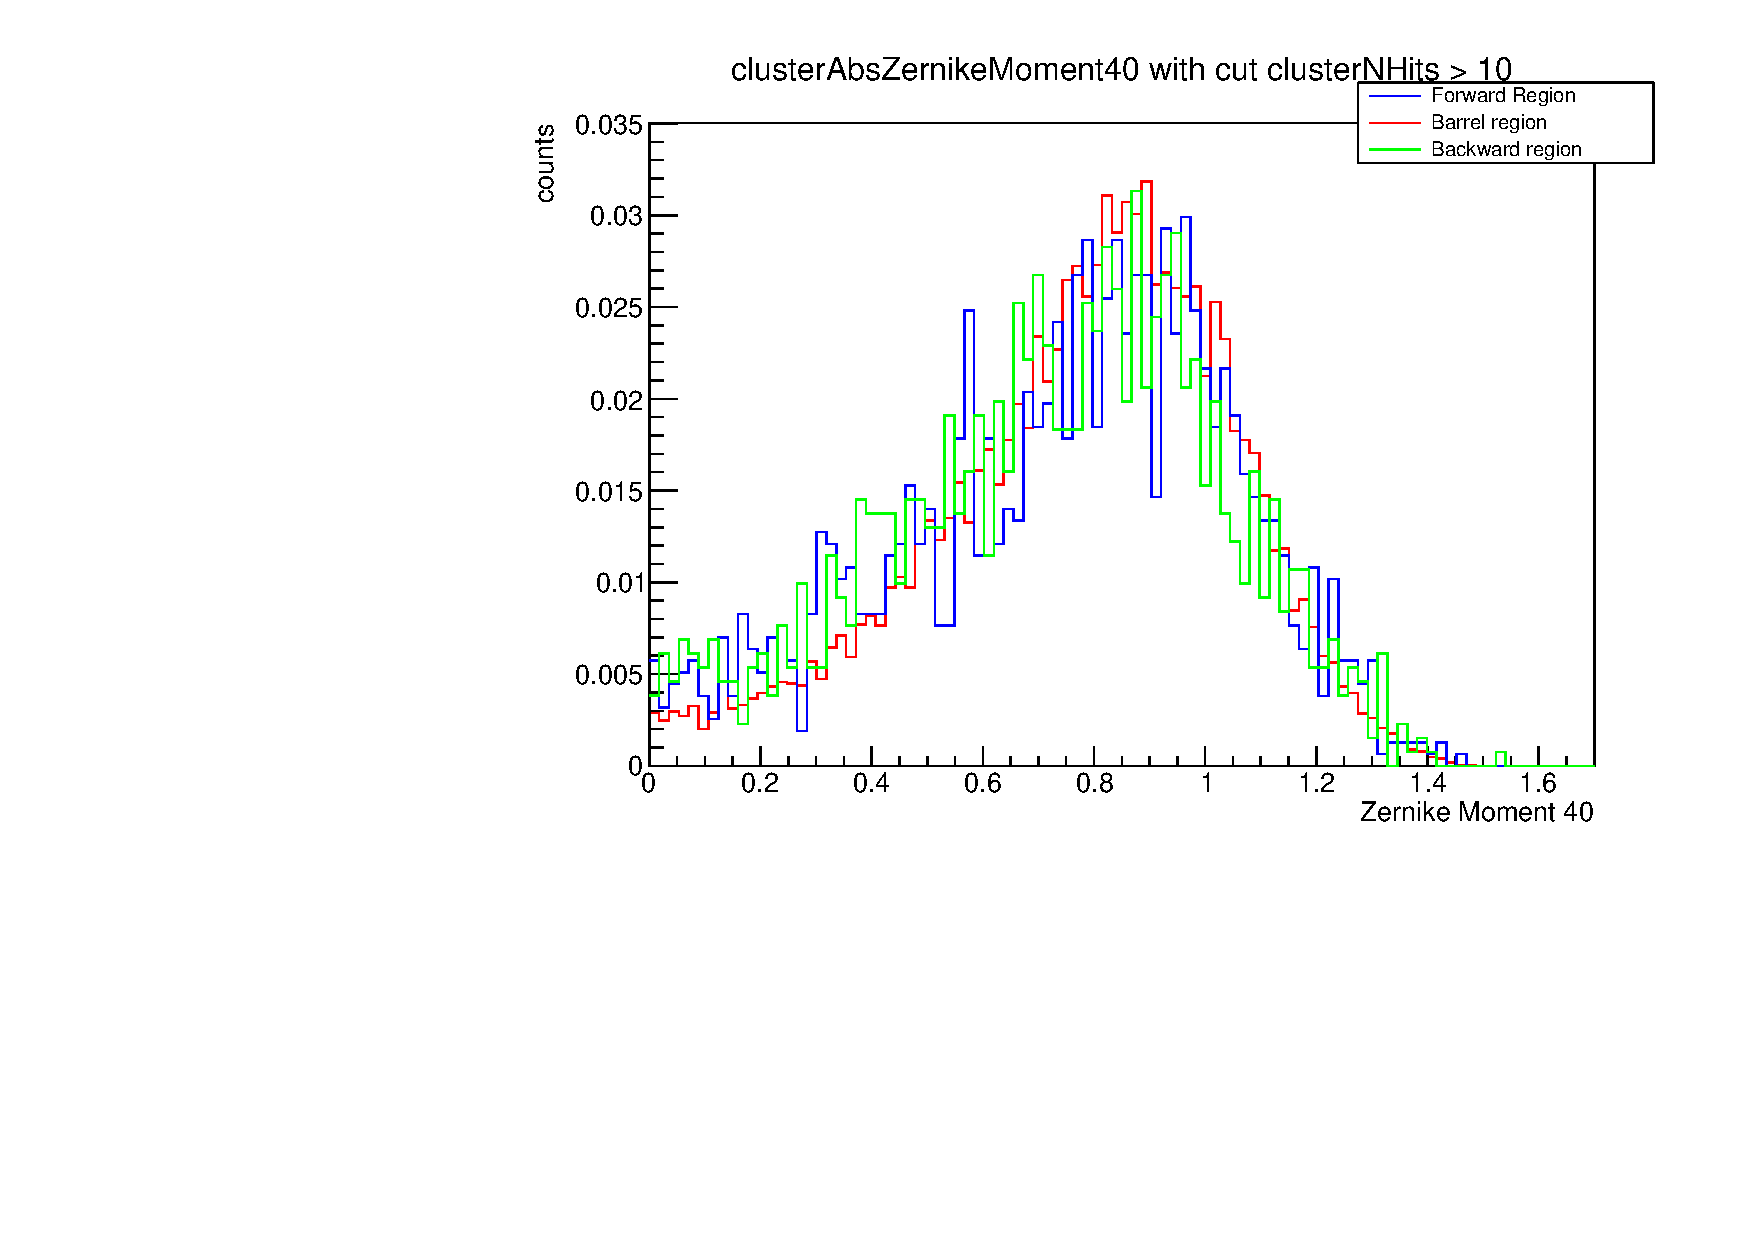
\includegraphics[width=0.49\textwidth]{nbar_MC/images/clusterAbsZernikeMoment40_nog_region.pdf}
    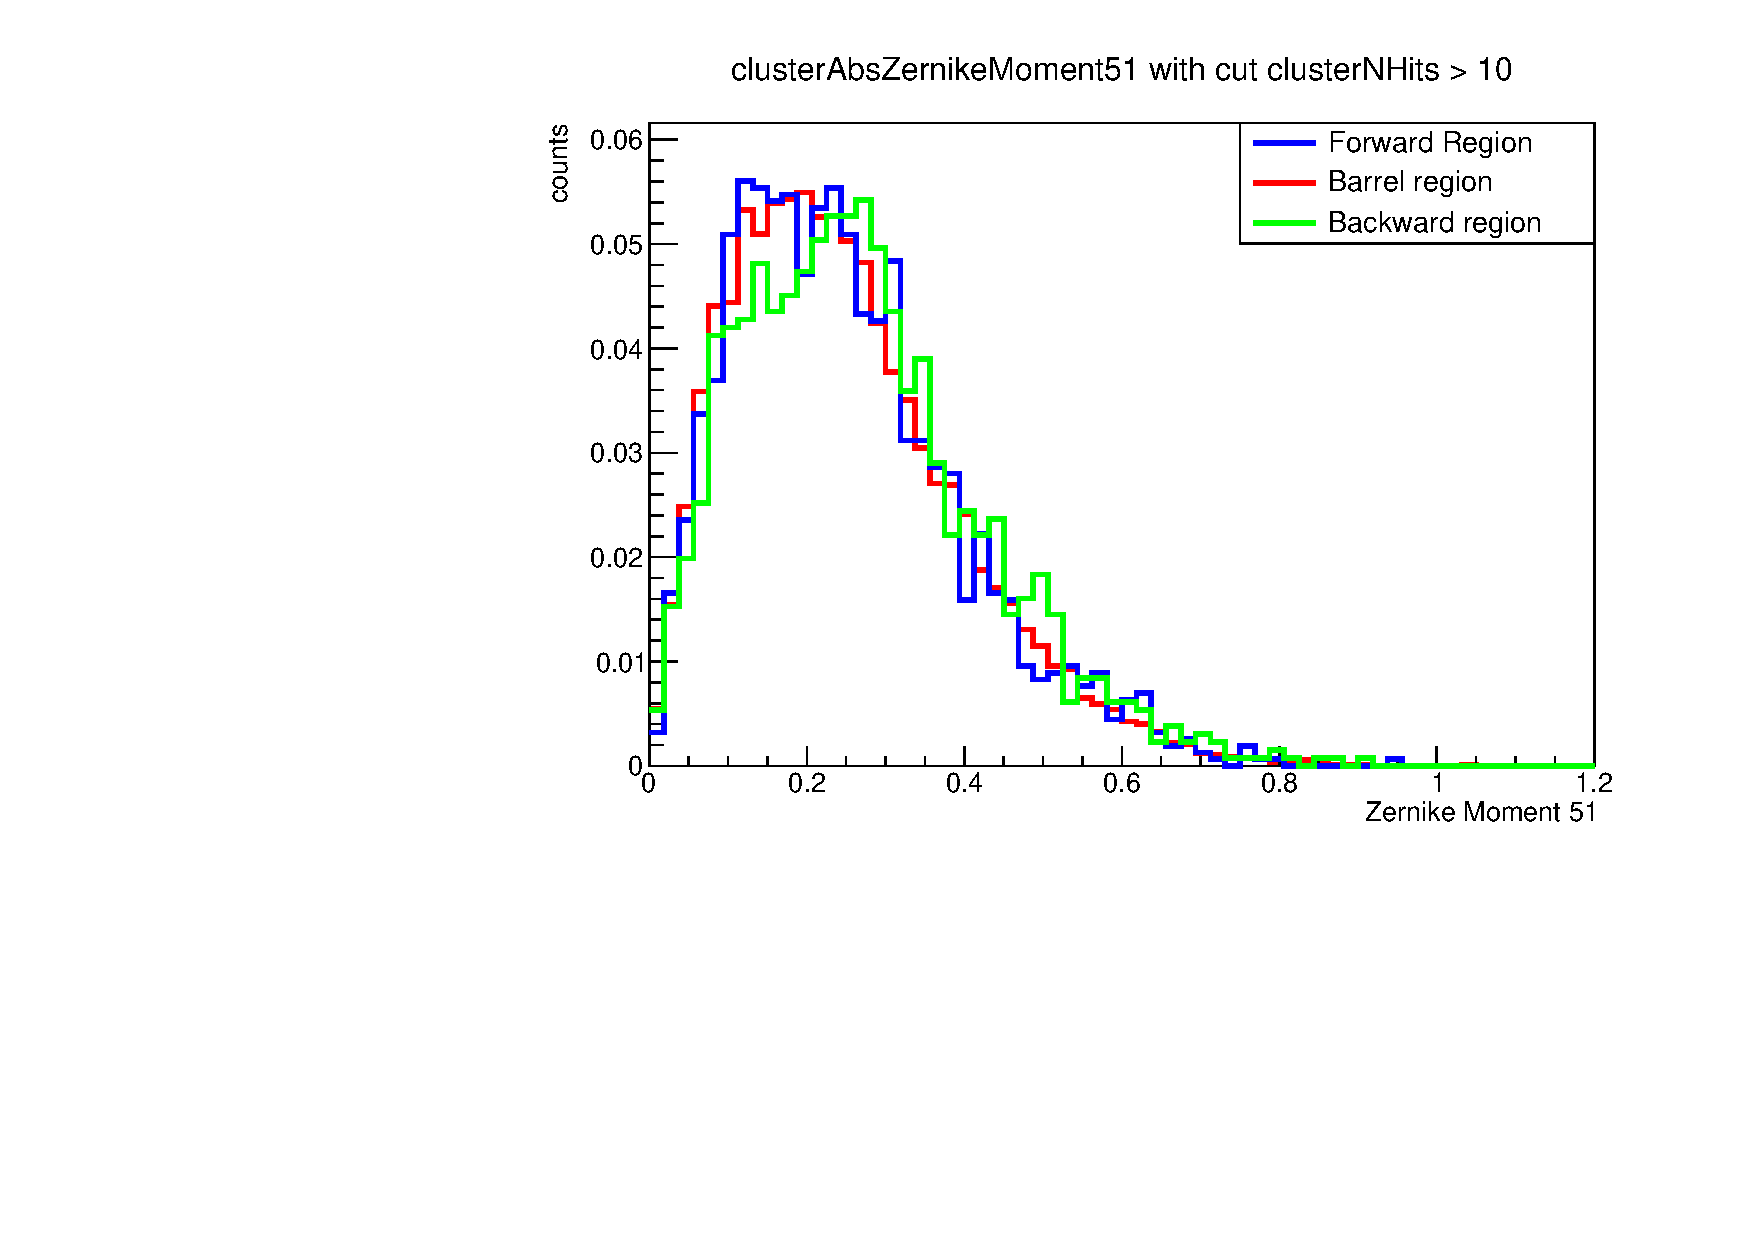
\includegraphics[width=0.49\textwidth]{nbar_MC/images/clusterAbsZernikeMoment51_nog_region.pdf}
    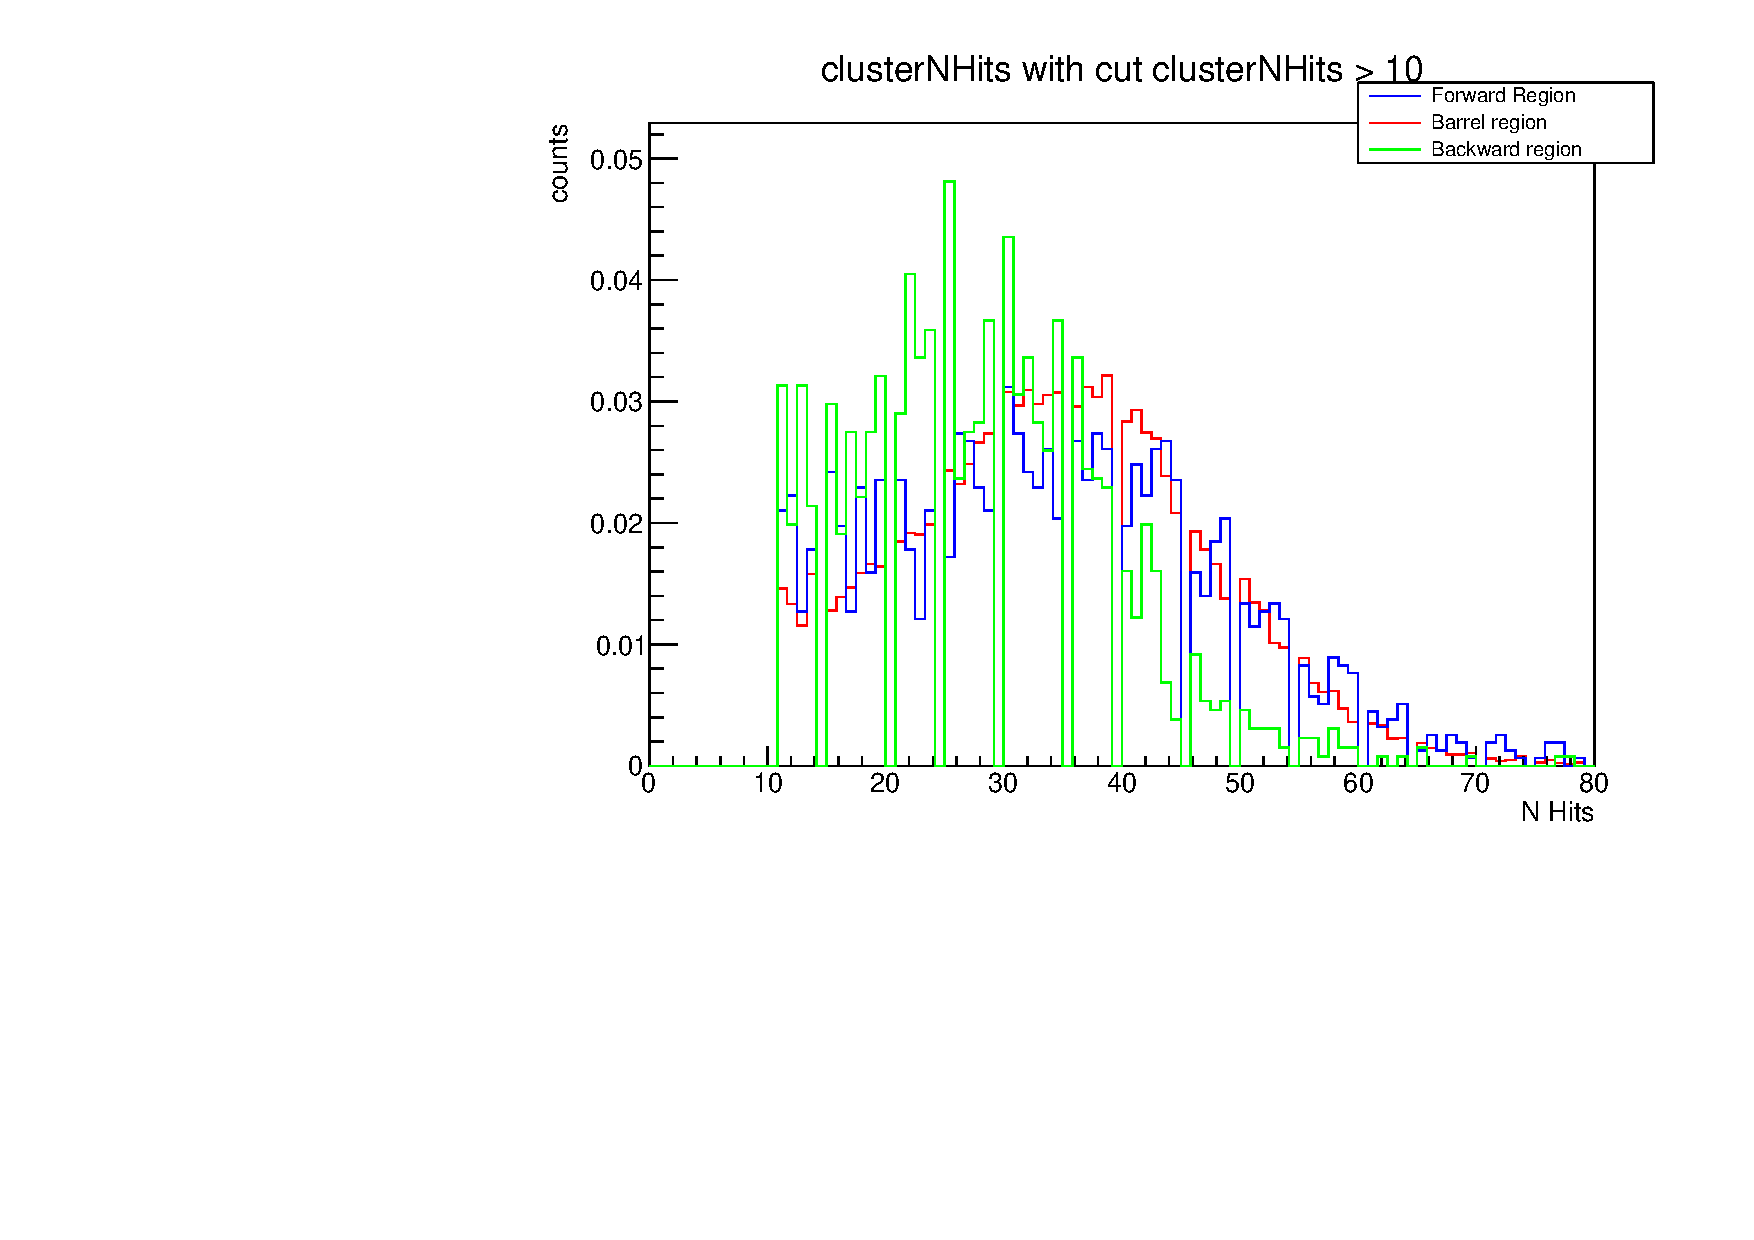
\includegraphics[width=0.49\textwidth]{nbar_MC/images/clusterNHits_nog_region.pdf}
   
     \caption{Comparison of reconstructed cluster variables for all $\bar{n}$ candidates in different ECL regions. The distributions are normalized to unit value}
      \label{fig:cluster_region}
\end{figure}

\subsection{Summary of Signal Channel Analysis}
The channel $e^+ \ + \  e^- \rightarrow p \ + \ \pi^- \ + \ \bar{n} $ has been studied, with both ISR and NO ISR emission. 
$\\$
$\\$
The recoil system $p\pi^-(\gamma_{ISR})$ is correctly reconstructed by the analysis, as evidenced by the peak above the anti-neutron mass in the recoil mass distribution. Furthermore, the kinematic distributions ($p$ and $\theta$) of the recoil system are consistent with those of generator-level $\bar{n}$ candidates, in both ISR and NO ISR cases. At reconstructed level, good agreement is observed in the $\theta$ distribution, while the reconstructed $\bar{n}$ candidate momentum shows underestimation and poor resolution compared to the recoil system momentum, as observed in correlations and residuals distributions. Furthermore, a low-momentum value structure is observed in reconstructed and generated momentum of $\bar{n}$ candidates compared to the recoil system momentum.
$\\$
$\\$
Therefore, energy loss occurs within ECL clusters, suggesting leakage processes such as cluster split-off and/or pre-showering effects. Ancestor studies reveal that photons related to $\bar{n}$ particles are often misidentified as main $\bar{n}$ candidates, accounting for the low-momentum structure observed. In fact, the ancestors momentum can be partially recovered when good Monte Carlo associations occur, showing good agreement with the recoil system momentum as well. A study of $\bar{n}$ production reveals that candidates with $\bar{n}$ ancestors are generated far from the IP, before the ECL (pre-showering) and within the ECL (cluster split-off).
$\\$
$\\$
Furthermore, a one-constraint (1C) Kinematic Fit was tested, revealing no significant improvement in the reconstructed recoil momentum and confirming that the recoil system was already optimally reconstructed by the analysis. 
$\\$
$\\$
Eventually, the reconstructed cluster variables associated with $\bar{n}$ candidates -such as cluster energy, lateral momentum, Zernike moments, etc.- were studied in the Monte Carlo signal sample. Similar structures to those observed in the momentum distributions were identified, particularly in the cluster energy and number of hits distributions.Therefore, ancestor studies confirm the momentum distribution observations: sub-clusters from secondary particles with $\bar{n}$ ancestry produce small-sized, low-energy structures in the cluster distributions.
$\\$
$\\$
In particular, a cut on the cluster number of hits yields reconstructed cluster variables closer to those expected from Monte Carlo $\bar{n}$ candidate selection, in both ISR and NO ISR cases.



\clearpage
\setcounter{subsection}{0} 
\part{Study of the Monte Carlo cocktail production}
This chapter is devoted to the study of Belle II Monte Carlo cocktail simulations. A Belle II "cocktail" MC production (typically generated with Pythia8) simulates all relevant physics channels simultaneously. Therefore, the analyzed channel $e^+e^- \rightarrow p\pi^-\bar{n}\,(\gamma_\text{ISR})$ is now embedded within all other background channels in the cocktail; the first task is to correctly reconstruct it amidst the surrounding backgrounds, studying the recoil mass distribution.
$\\$
To achieve this, a first attempt uses the $u\bar{u}$ cocktail production. Further selection criteria are developed to properly isolate the signal in the recoil mass distribution.
$\\$
Afterwards, the full Belle II $q\bar{q}$ ($u\bar{u}$, $d\bar{d}$, $c\bar{c}$, $s\bar{s}$) production is analyzed, discussing the corresponding $\bar{n}$ candidates cluster variables.
$\\$
The Feynman diagram of $e^+e^- \rightarrow q \bar{q}$ is shown in Fig.~\ref{fig:Feynman_qqbar}.

\begin{figure}[H]
    \centering
    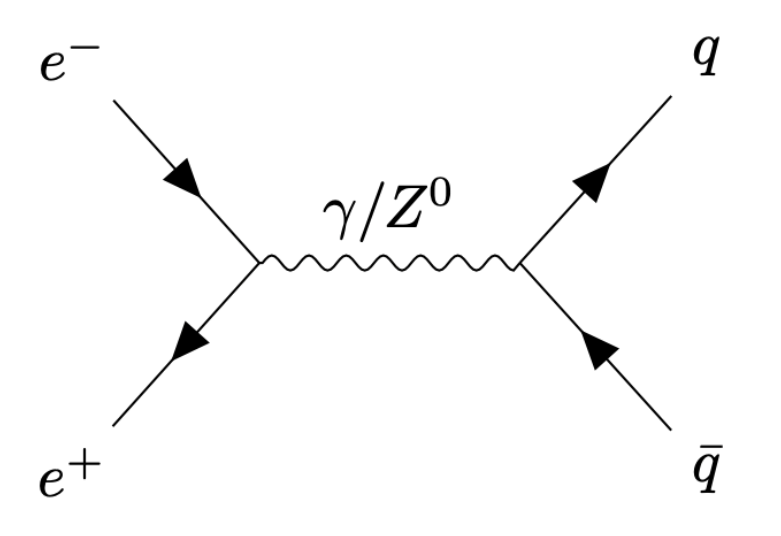
\includegraphics[width=0.45\textwidth]{nbar_cocktail/images/qqbar_diag}
    \caption{Tree level Feynman diagram of $e^+ e^- \to q \bar{q}$}
    \label{fig:Feynman_qqbar}
\end{figure}

\subsection{Types of processes at the Belle experiment enviroment}
Many processes can occur during an $e^+e^-$ collision. These may mimic the selected signal and be accidentally reconstructed as signal events, though they represent background processes.
$\\$
The $\Upsilon(4S)$ production occurs at $\sqrt{s} = 10.58$ GeV, yielding $\Upsilon(4S) \rightarrow BB$ processes. The $B^+B^-$ and $B^0 \bar{B}^0$ final states  are referred to as charged and neutral $B \bar{B}$ pairs, respectively.
$\\$
The $e^+e^- \to q\bar{q}$ ($q = u,d,s,c$) processes, known as continuum production, also occur. There are $e^+e^- \to l^+l^- (\gamma)$ and $e^+e^- \to l^+l^-l^-l^+$, with $l = (e,\mu,\tau)$, that are low multiplicity processes. The cross section distribution \cite{BelleIIPhysicsBook2019} of $e^+ e^- \rightarrow hadrons$ process is shown in Fig.\ref{fig:belleii_processes}.

\begin{table}[h]
\centering
\begin{tabular}{l r}
Process & Cross section (nb) \\
$e^+e^- \to \Upsilon(4S)$ & 1.10 \\
$e^+e^- \to u\bar{u} (\gamma)$ & 1.61 \\
$e^+e^- \to d\bar{d} (\gamma)$ & 0.40 \\
$e^+e^- \to s\bar{s} (\gamma)$ & 0.38 \\
$e^+e^- \to c\bar{c} (\gamma)$ & 1.30 \\
$e^+e^- \to \tau^+\tau^- (\gamma)$ & 0.92 \\
$e^+e^- \to e^+e^- (\gamma)$ & 300 \\
$e^+e^- \to \mu^+\mu^- (\gamma)$ & 1.15 \\
$e^+e^- \to \gamma \gamma (\gamma)$ & 4.99 \\
$e^+e^- \to e^+e^-e^+e^-$ & 39.7 \\
$e^+e^- \to e^+e^-\mu^+\mu^-$ & 18.9 \\
\end{tabular}
\end{table}

\begin{figure}[H]
    \centering
    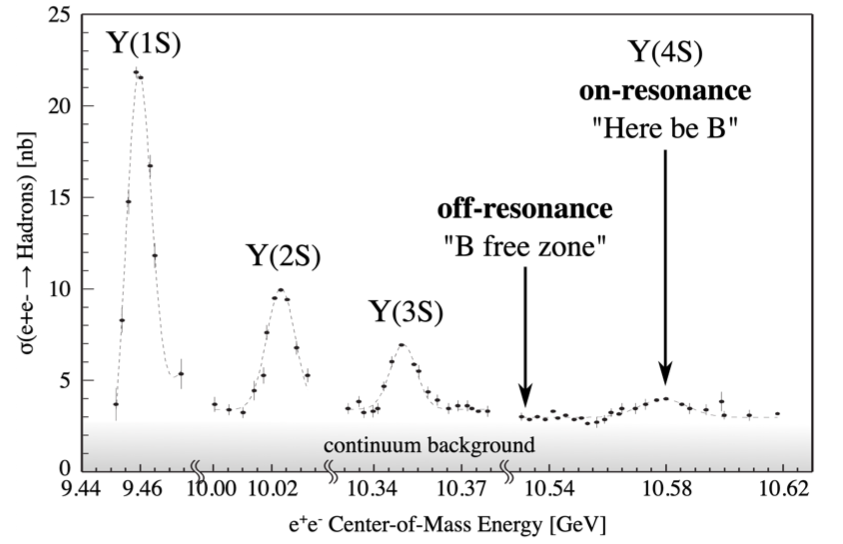
\includegraphics[width=0.9\textwidth]{nbar_cocktail/images/BelleII_processes}
    \caption{Cross section of $e^+ e^- \rightarrow hadrons$, in $\Upsilon$ resonances energy region. The $\Upsilon(1S)$ resonance is very narrow, while the $\Upsilon(4S)$ one is broader and lower.}
    \label{fig:belleii_processes}
\end{figure}

\subsection{Selections criteria}
To follow the same approach as used in the signal sample analysis, the recoil mass is first studied using the complete $u\bar{u}$ cocktail production, which corresponds to an integrated luminosity of $\sim 1429.23 \ fb^{-1}$. The following event selections have been applied:
\begin{enumerate}
\item $p$: $protonID > 0.9$ and $dr<1$ cm and $|dz|<3$ cm;
\item $\pi^-$: $pionID > 0.1$ and $dr<1$ cm and $|dz|<3$ cm;
\item $\bar{n}$: neutral clusters from ECL and number of hits $> 10$ and energy $<3$ GeV;
\item Recoil system: $0 \ GeV/c^2 <recoil \ mass < 2 \ GeV/c^2$;
\item $\alpha <0.20$ rad $\sim 11.5 ^{\circ}$;
\item No further charged particles in the Rest of Event (ROE).
\end{enumerate}
$\\$
Four additional cuts are applied beyond those used for the signal sample, such as cluster number of hits $> 10$ GeV, $\alpha <0.20$ rad, the request of no further charged particles in the Rest of Event (ROE) and the energy of the neutral cluster associated to $\bar{n}$ candidates must be less then 3 GeV.
$\\$
The first cut arises from observations in the previous chapter; to achieve a proper selection of neutral clusters associated with anti-neutron candidates -reducing cluster split-off and pre-showering contributes- a requirement on the number of lighted crystals is applied. 
$\\$
The second cut allows a stricter selection of anti-neutron candidates through a smaller $\alpha$ angle. $\alpha$ is defined as the 3D angle between the recoil vector direction and the neutral cluster associated with the $\bar{n}$. As will be explained later, this threshold can be lowered further.
$\\$
To explain the third cut, the concept of \textbf{Rest of Event} (ROE) must first be introduced. The ROE is built around the reconstructed target particles and consists of all other particles in the Rest of Event. In the present case, the reconstructed particles are $p, \pi^-, \bar{n}$ (and $\gamma_{ISR}$); therefore, the ROE includes all particles outside this reconstructed system. Consequently, the third selection criterion requires that no charged particles -i.e. tracks associated with charged particles- be present in the Rest Of Event, providing a cleaner event reconstruction. A Feynman diagram with ROE is shown in Fig.\ref{fig:ROE_feynman}.

\begin{figure}[H]
    \centering
    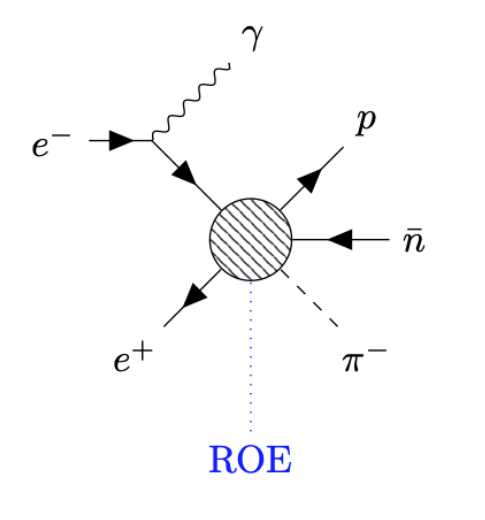
\includegraphics[width=0.45\textwidth]{nbar_cocktail/images/ROE_diag}
    \caption{Feynman diagram of the channel of interest, with the Rest of Event ROE made of a variable amount of particles.}
    \label{fig:ROE_feynman}
\end{figure}

The fourth cut arises from cluster energy studies performed on the first chunk of $u\bar{u}$ cocktail production, corresponding to $\sim 215 fb^{-1}$. The $\bar{n}$ list can be affected by several mis-identified $\gamma_\text{ISR}$. In order to study this phenomenon, the Monte Carlo ISR flag (\textbf{mcISR}) can be used to separate the two contributions in reconstructed $\bar{n}$ list. The mcISR variable is a Monte Carlo flag that indicates whether a particle is an ISR particle or not;
if mcISR = 0, the reconstructed particle is not an ISR photon; if mcISR = 1, the reconstructed particle is an ISR photon mis-identified as an anti-neutron. The obtained cluster energy distribution for $\bar{n}$ candidates, in $u\bar{u}$ chunk1 cocktail production, is shown in figure ~\ref{fig:E_isr_uubar_c1}.
$\\$
Two structures, at $\sim 4$ GeV and $\sim 6$ GeV, due to $\gamma_{ISR}$ mis-identified as anti-neutrons, arise. In order to remove them, a cut on cluster energy, such as those discussed, is mandatory.
\begin{figure}[h]
    \centering
    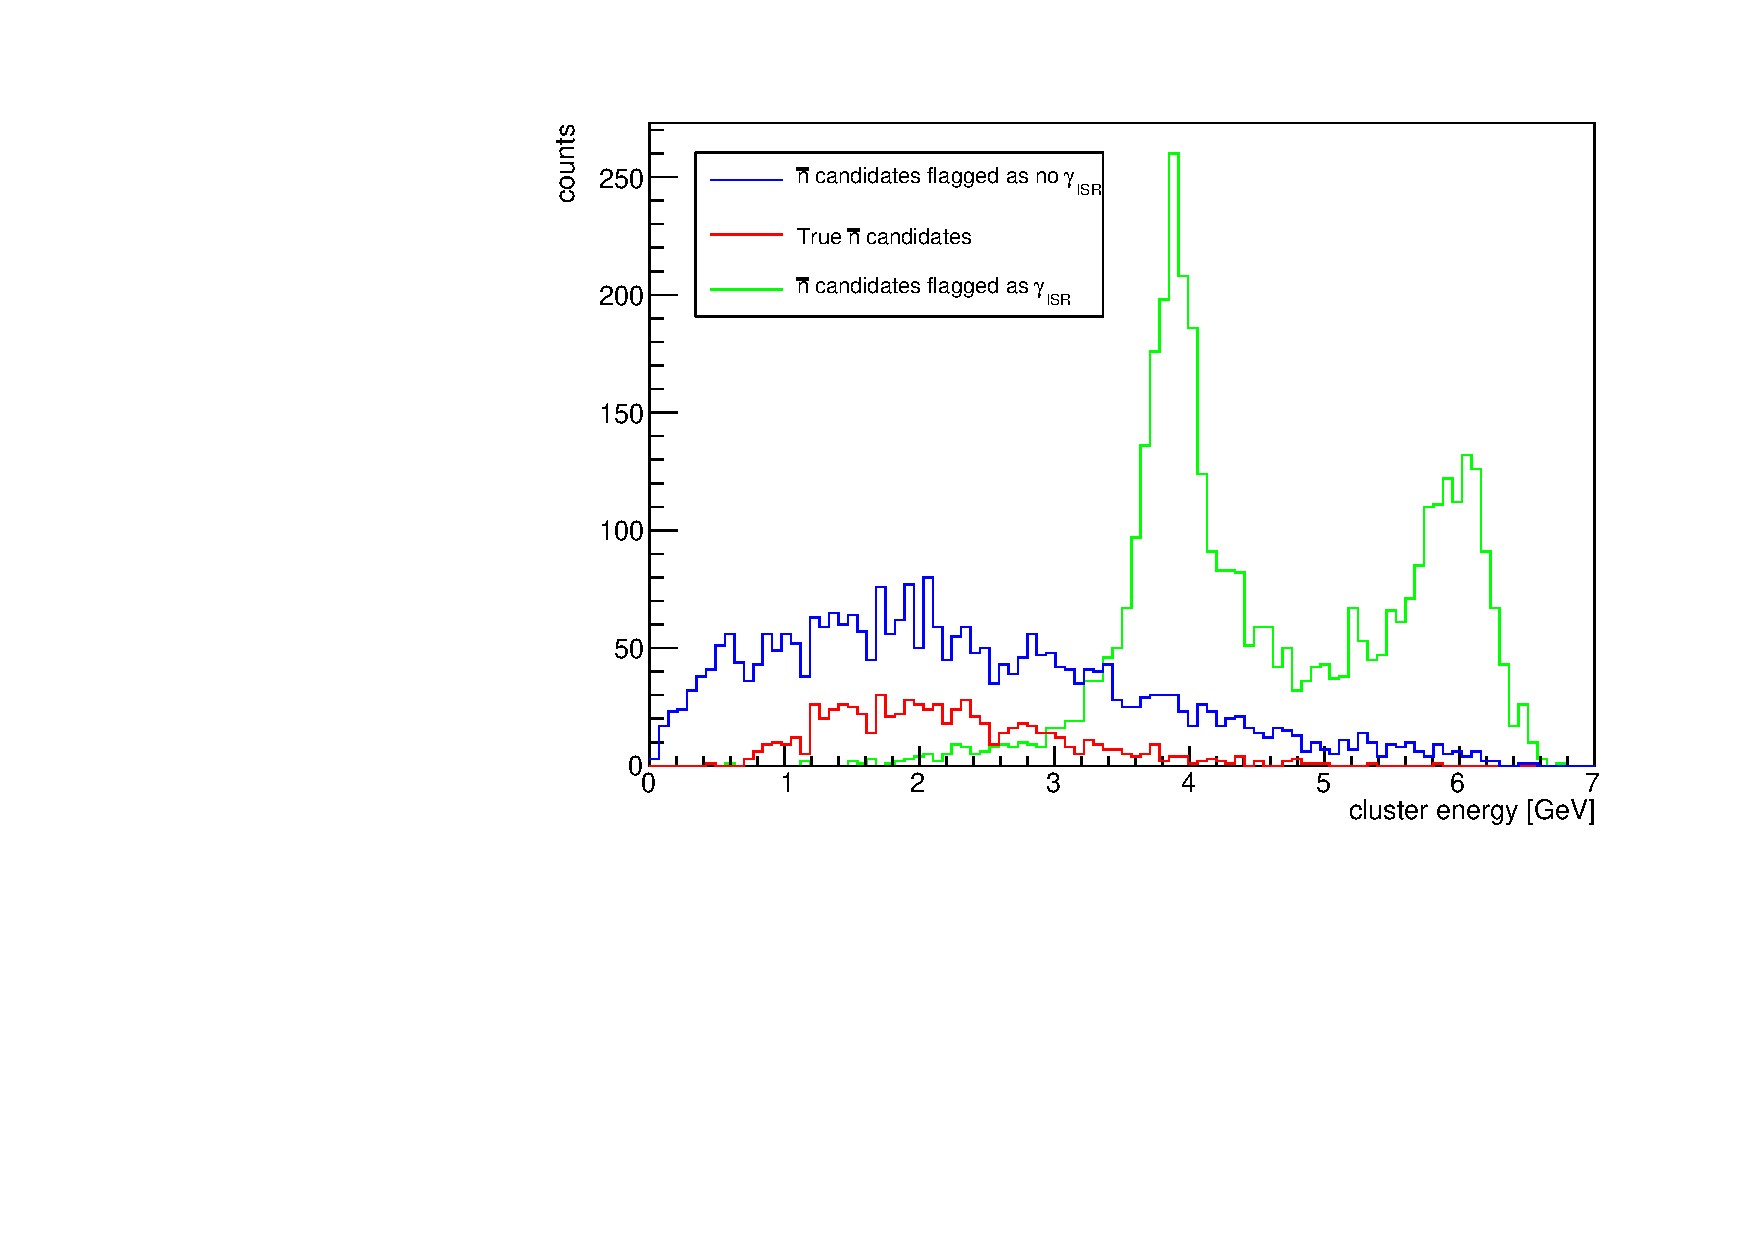
\includegraphics[width=0.80\textwidth]{nbar_cocktail/images/clusterEnergy_isr}
    \caption{Cluster energy distribution of $\bar{n}$ candidates, divided by the Monte Carlo ISR flag (\texttt{mcISR}), in $u\bar{u}$ chunk1 cocktail production. If \texttt{mcISR} = 0 (blue), the reconstructed particle is not an ISR photon. If \texttt{mcISR} = 1 (red), the reconstructed particle is an ISR photon. \texttt{mcISR} is a Monte Carlo information.}
    \label{fig:E_isr_uubar_c1}
\end{figure}
$\\$
However, $\gamma$ radiation represents one of the most abundant produced particles in HEP experiments such as Belle II, making a major contribution to the background. In addition to the ISR ($E \sim 10$ MeV - $5$ GeV, Fig.~\ref{fig:isr_distro}) and FSR ($E< 10$ MeV) radiation described above, bremsstrahlung ($E < 50$ MeV) and secondary photons -such as those from $\pi^0 \rightarrow \gamma \gamma$ decays  ($E < 400$ MeV)- are also present. Therefore, NO ISR channel where the recoil system is made of  $p, \pi^-$ should represents a cleaner system to reconstruct than the ISR one where the recoil system is made of  $p, \pi^-, \gamma$, since several background $\gamma$'s can be mis-identified as the ISR photon, which must be accounted for in the recoil system.
$\\$
In order to compare the feasibility of selecting the channel in both ISR and NO ISR cases separately, the recoil mass distribution must be first studied using the same selection criteria. The better the selection of the signal from the background, the more consistent the shower shape variables will be for neutral clusters associated with $\bar{n}$ candidates.

\subsection{Recoil mass in $u\bar{u}$ cocktail production (NO ISR case)}
The recoil mass distribution obtained from the $u\bar{u}$ cocktail is first studied in NO ISR case. If the recoil system $p, \pi^-$ is properly reconstructed among all possible background channels, then a peak should be observed at the anti-neutron rest mass ($939.5$~MeV/$c^2$). The obtained result is shown in Fig.~\ref{fig:mRec_nog_020}.
\begin{figure}[h]
    \centering
    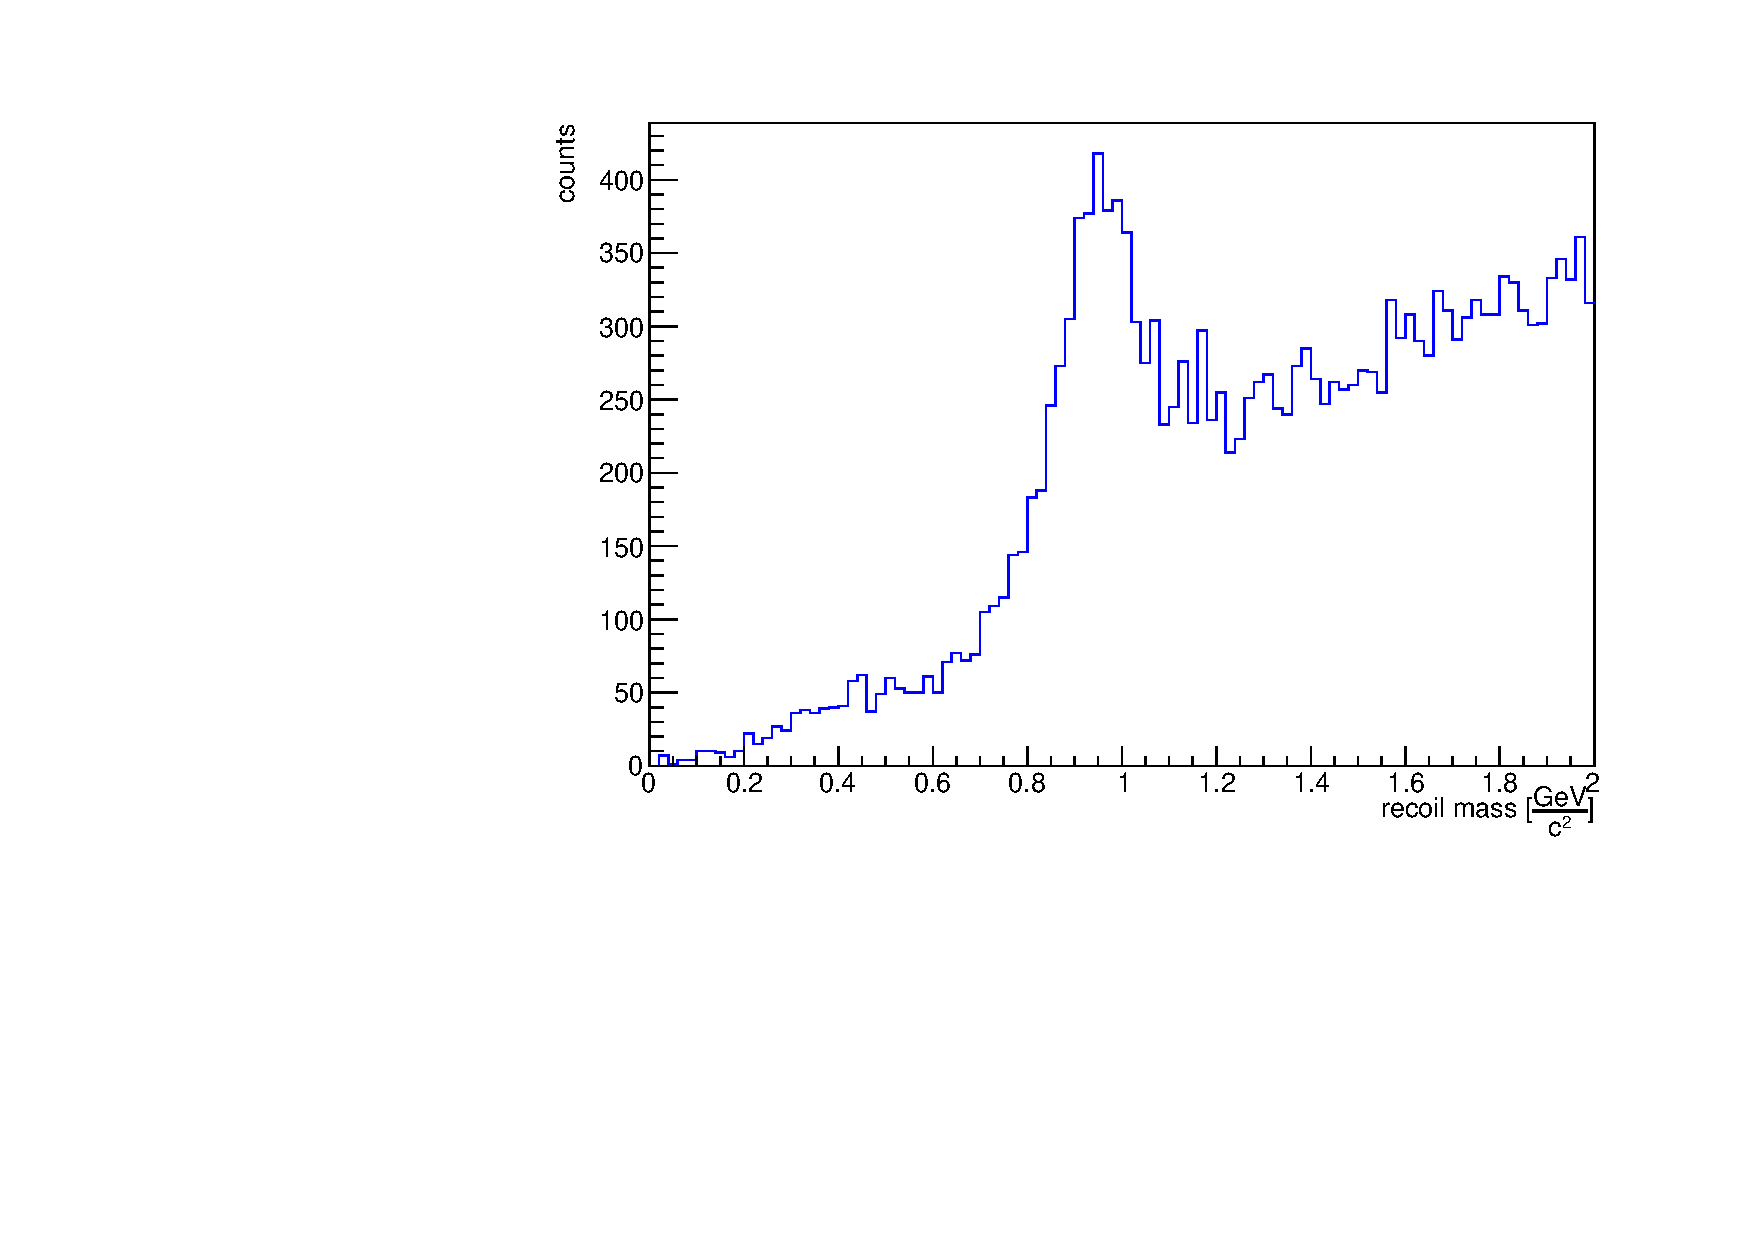
\includegraphics[width=0.80\textwidth]{nbar_cocktail/images/recoil_mass_nog_020}
    \caption{Reconstructed $p, \pi^-$ recoil mass distribution in $u\bar{u}$ Monte Carlo cocktail, NO ISR case.}
    \label{fig:mRec_nog_020}
\end{figure}

A distinct structure is observed above the $\bar{n}$ mass value, suggesting that the selected channel is properly reconstructed. For a cleaner comparison between the signal channel and background components, the TopoAna output can be consulted in Fig.~\ref{fig:topo_nog_020}. TopoAna does not account for particle-matter interactions; thus, all displayed particles originate directly from the $e^+e^-$ collision at the IP.
\begin{figure}[h]
    \centering
    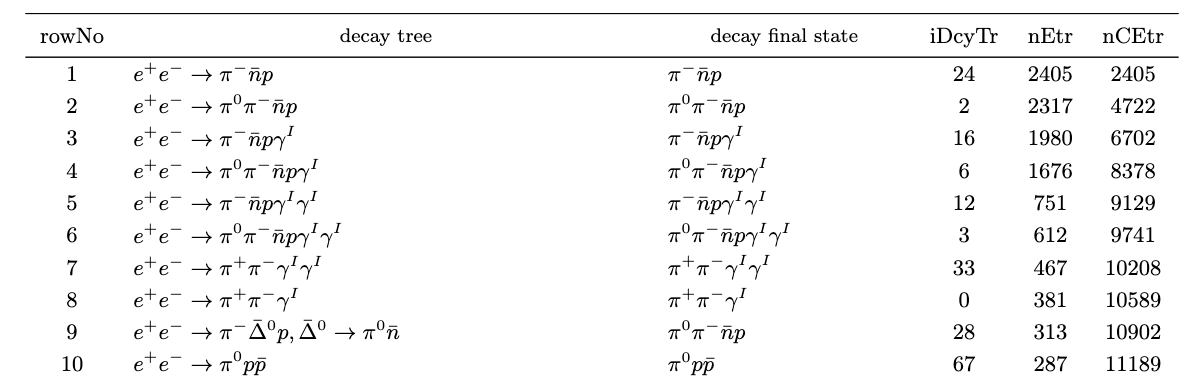
\includegraphics[width=1\textwidth]{nbar_cocktail/images/topoana_nog_020}
    \caption{First 10 channels of the TopoAna output in $u\bar{u}$ Monte Carlo cocktail, showing the different channel contributes, NO ISR case.}
    \label{fig:topo_nog_020}
\end{figure}

Accessing the Monte Carlo information from TopoAna, the main contribution comes from the signal channel with $p \pi^- \bar{n}$ in the final state, immediately followed by the one with $p \pi^- \bar{n} \pi^0$ in the final state. Further contribution arise from $p \pi^- \bar{n} \gamma_{ISR}$, which could be interpreted as signal, even if, in NO ISR case, the $\gamma_{ISR}$ is not explicitly reconstructed within the recoil system. The fourth contribute is due to the one with $p \pi^- \bar{n} \pi^0 \gamma_{ISR}$ and so on. The contributions are sorted from most to least abundant.

\subsubsection{Recoil mass components analysis}
The recoil mass distribution components can be studied by correlating the ntuple information obtained from the steering file with that produced by the TopoAna program. 
$\\$
Each channel is identified by its own \texttt{iDcyTr} (index of the decay tree), which allows one to represent the contribution of a given channel (or a combination of channels) to a specific variable, such as the recoil mass of the system $p \pi^-$.
$\\$
The components are therefore denoted as follows:
\begin{enumerate}
\item $e^+ e^- \rightarrow \pi^- \bar{n} p$ (iDcyTr == 24);
\item $e^+ e^- \rightarrow \pi^0 \pi^- \bar{n} p$ (iDcyTr == 2);
\item $e^+ e^- \rightarrow \pi^- \bar{n} p \gamma_{ISR}$ (iDcyTr == 16);
\item $e^+ e^- \rightarrow \pi^0 \pi^- \bar{n} p \gamma_{ISR}$ (iDcyTr == 6);
\item $e^+ e^- \rightarrow$ other.
\end{enumerate}
The obtained stacked component to the recoil mass are shown in figure ~\ref{fig:mRecComps_nog_020}.
\begin{figure}[h]
    \centering
    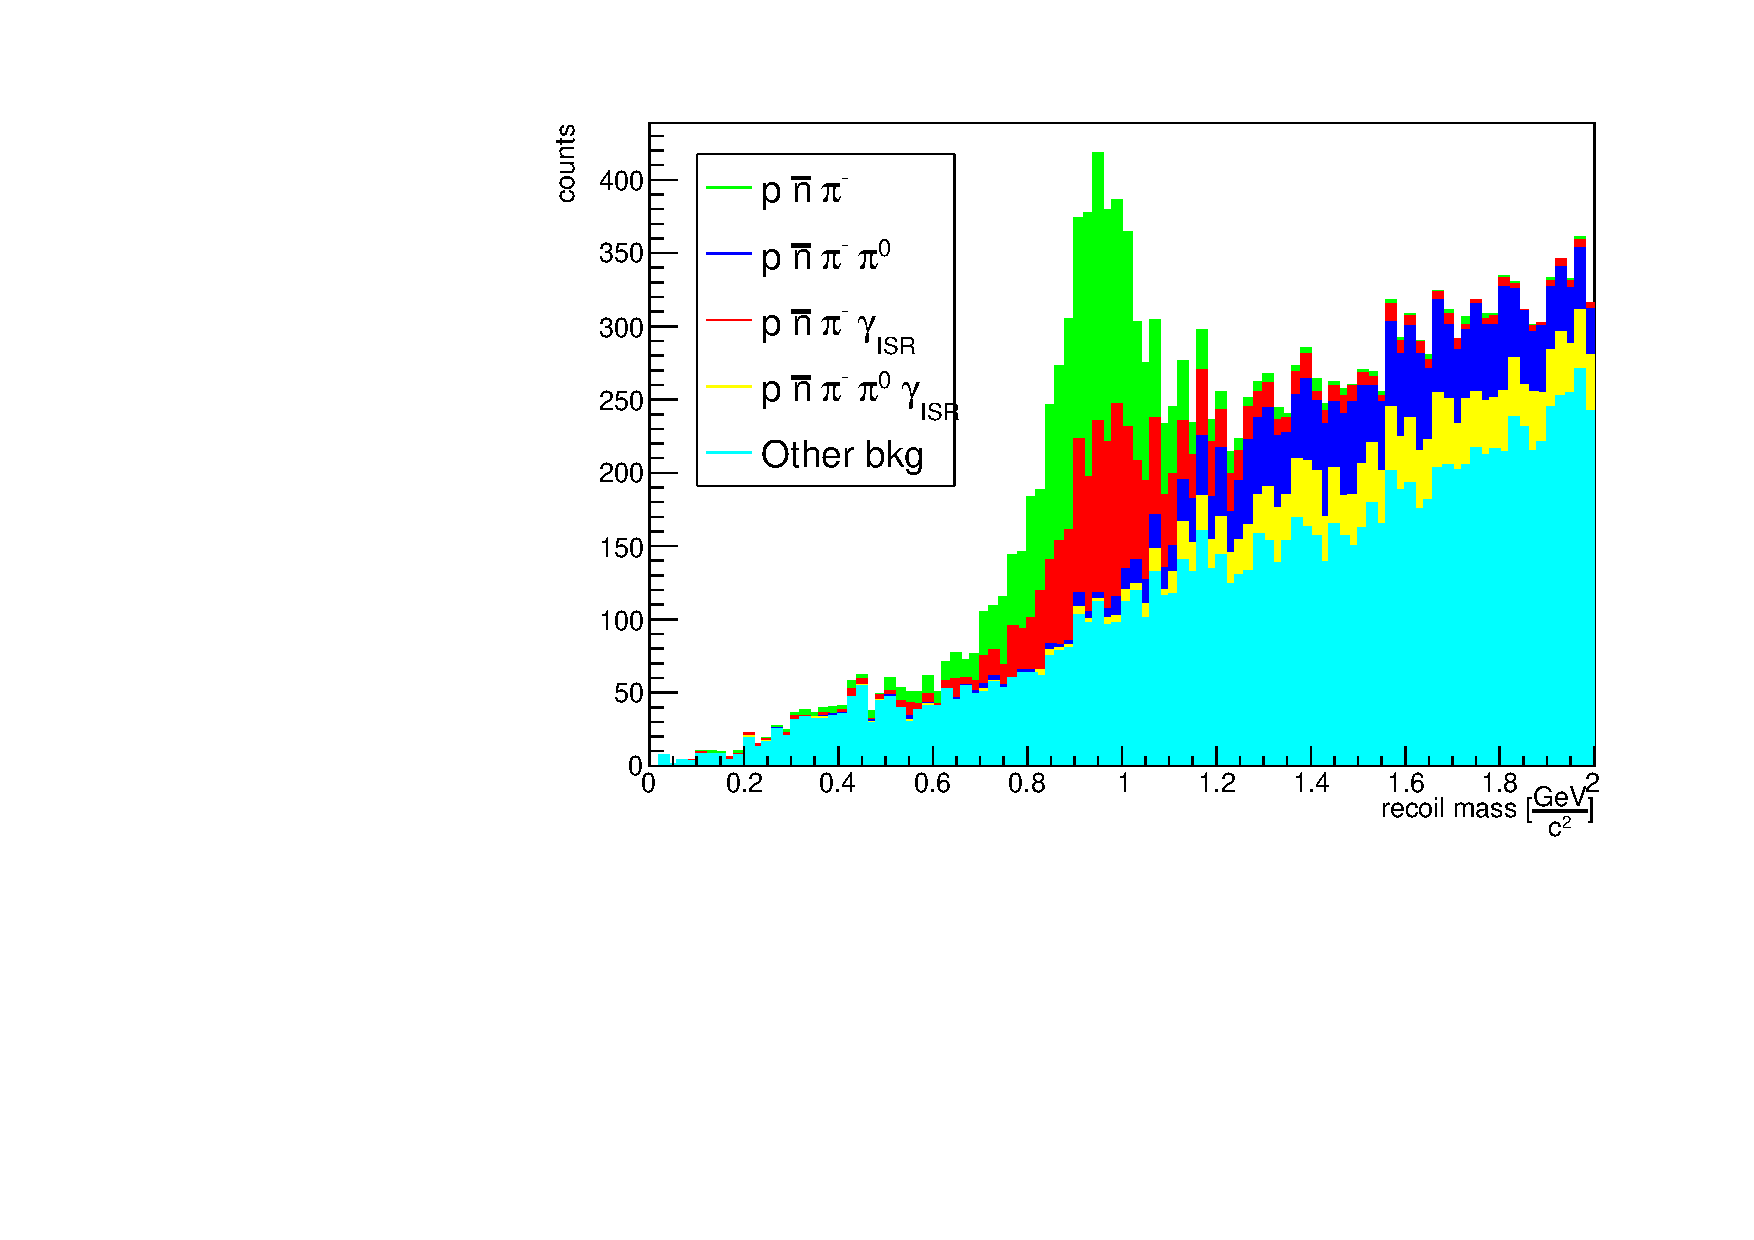
\includegraphics[width=0.90\textwidth]{nbar_cocktail/images/recoilM_comps_nog_020}
    \caption{$p, \pi^-$ recoil mass distribution in $u\bar{u}$ Monte Carlo cocktail, displaying each stacked component contribution, NO ISR case. Green: $\pi^- \bar{n} p$ channel. Blue: $\pi^0 \pi^- \bar{n} p$ channel. Red: $\pi^- \bar{n} p \gamma_{ISR}$. Yellow: $\pi^0 \pi^- \bar{n} p \gamma_{ISR}$ channel. Cyan: other channels.}
    \label{fig:mRecComps_nog_020}
\end{figure}
Defining the \emph{Signal Region} as the interval $[0.8, 1.2]$ GeV, it can be observed that contributions from the channel with iDcyTr = 2 predominantly lie to the right of the signal region. This is expected, as the recoil system computation excludes the $\pi^0$, leading to a higher recoil mass. Same conclusions can be made for the with iDcyTr = 6. 
$\\$
The signal channel (iDcyTr = 24) predominantly populates the signal region. The $\pi^- \bar{n} p \gamma_{ISR}$ channel (iDcyTr = 16) also mainly populates the signal region, indicating that the $\gamma_{ISR}$ is negligible and has minimal impact on the recoil mass, as shown by the ISR energy distribution in Fig.~\ref{fig:isr_distro}. This can be directly observed from the single contribute from these two channels displayed in Fig.~\ref{fig:mRecComps_nog_020_0e3}. The contributions from the remaining channels represent a flat background without discernible structures.
\begin{figure}[H]
    \centering
    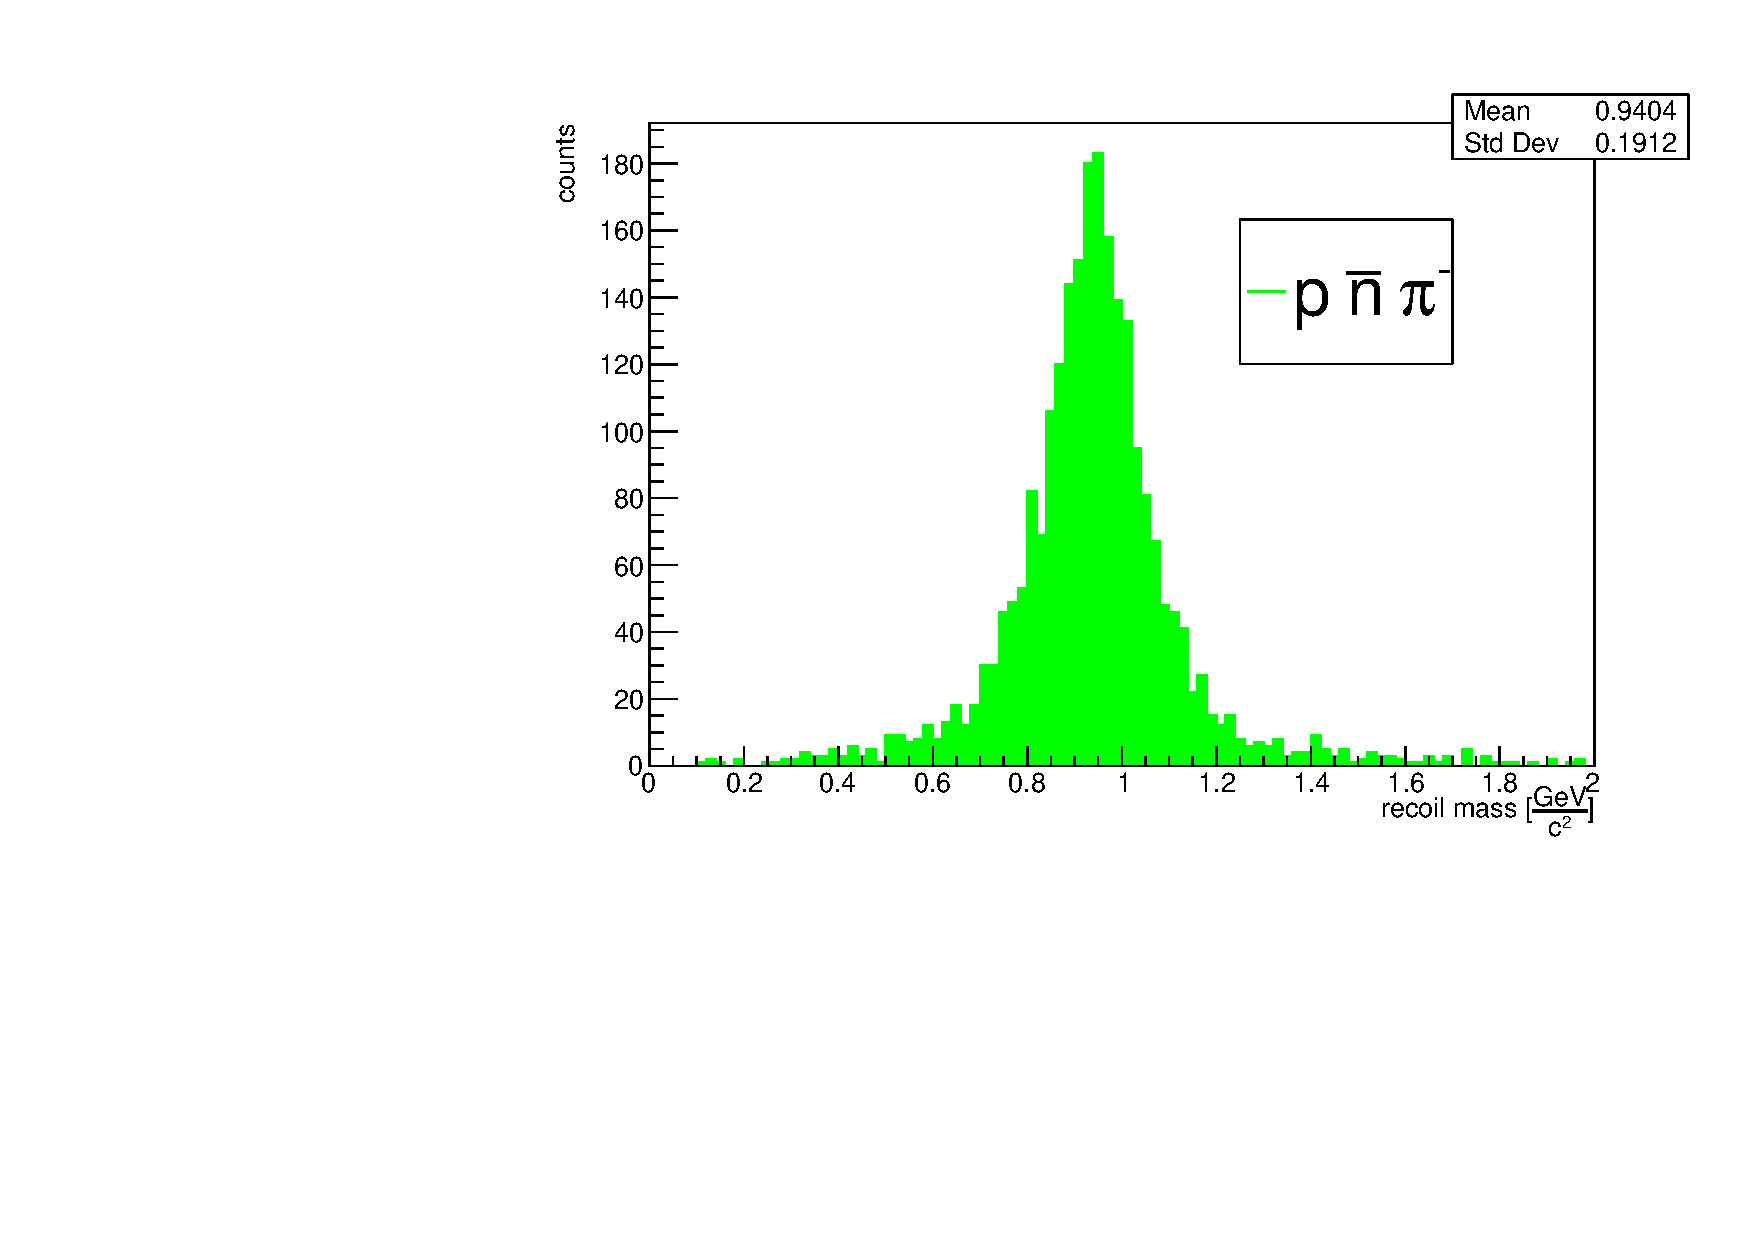
\includegraphics[width=0.49\textwidth]{nbar_cocktail/images/recoilM_comp0_nog_020}
    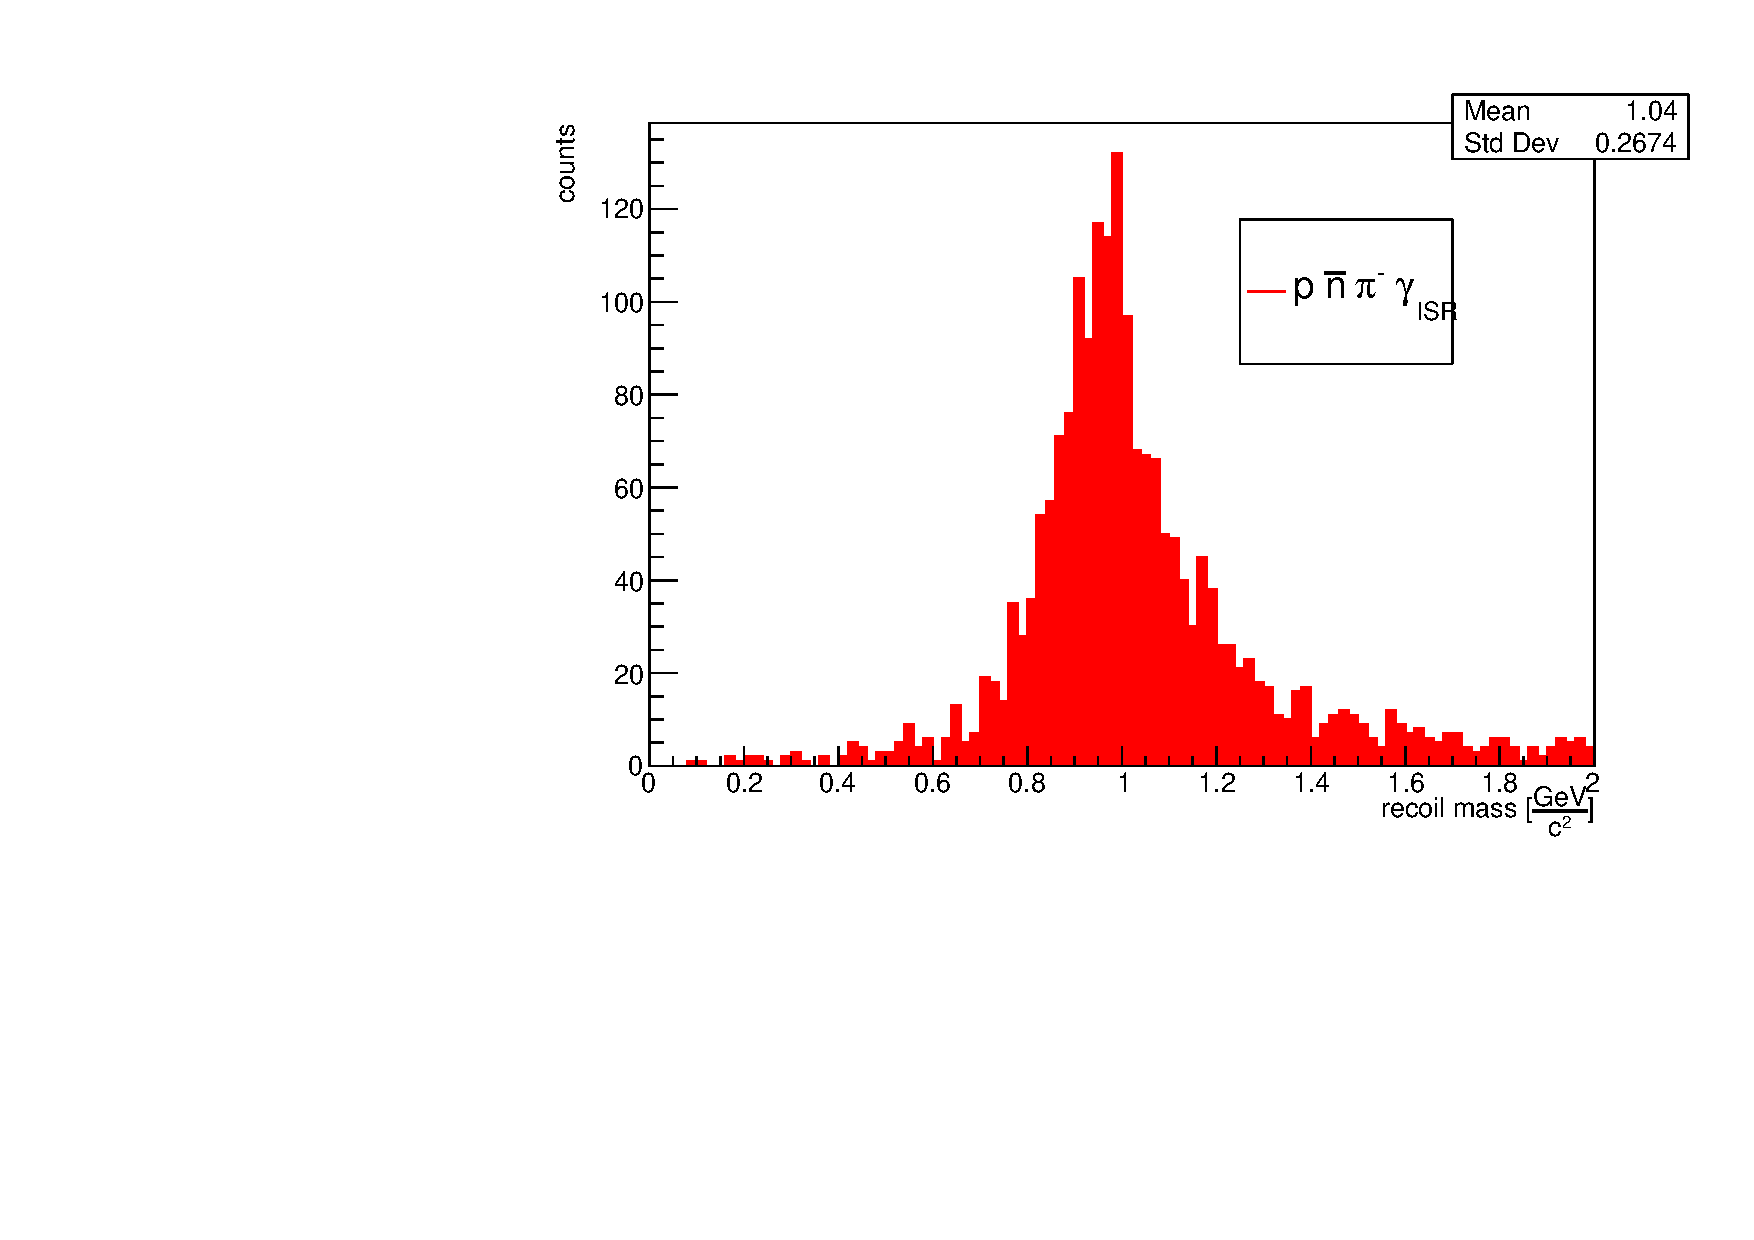
\includegraphics[width=0.49\textwidth]{nbar_cocktail/images/recoilM_comp3_nog_020}
    \caption{ (green) $p, \pi^-$ recoil mass and (red) $p, \pi^-, \gamma_{ISR}$ recoil mas distribution in $u\bar{u}$ Monte Carlo cocktail.}
    \label{fig:mRecComps_nog_020_0e3}
\end{figure}
$\\$
Thus, despite the $\gamma_{ISR}$ not being directly reconstructed, the $\pi^- \bar{n} p \gamma_{ISR}$ channel (iDcyTr = 16) can be considered a signal channel. This leads to the recoil mass composition shown in Fig.~\ref{fig:mRecComps_nog_020_0+3}.
\begin{figure}[h]
    \centering
    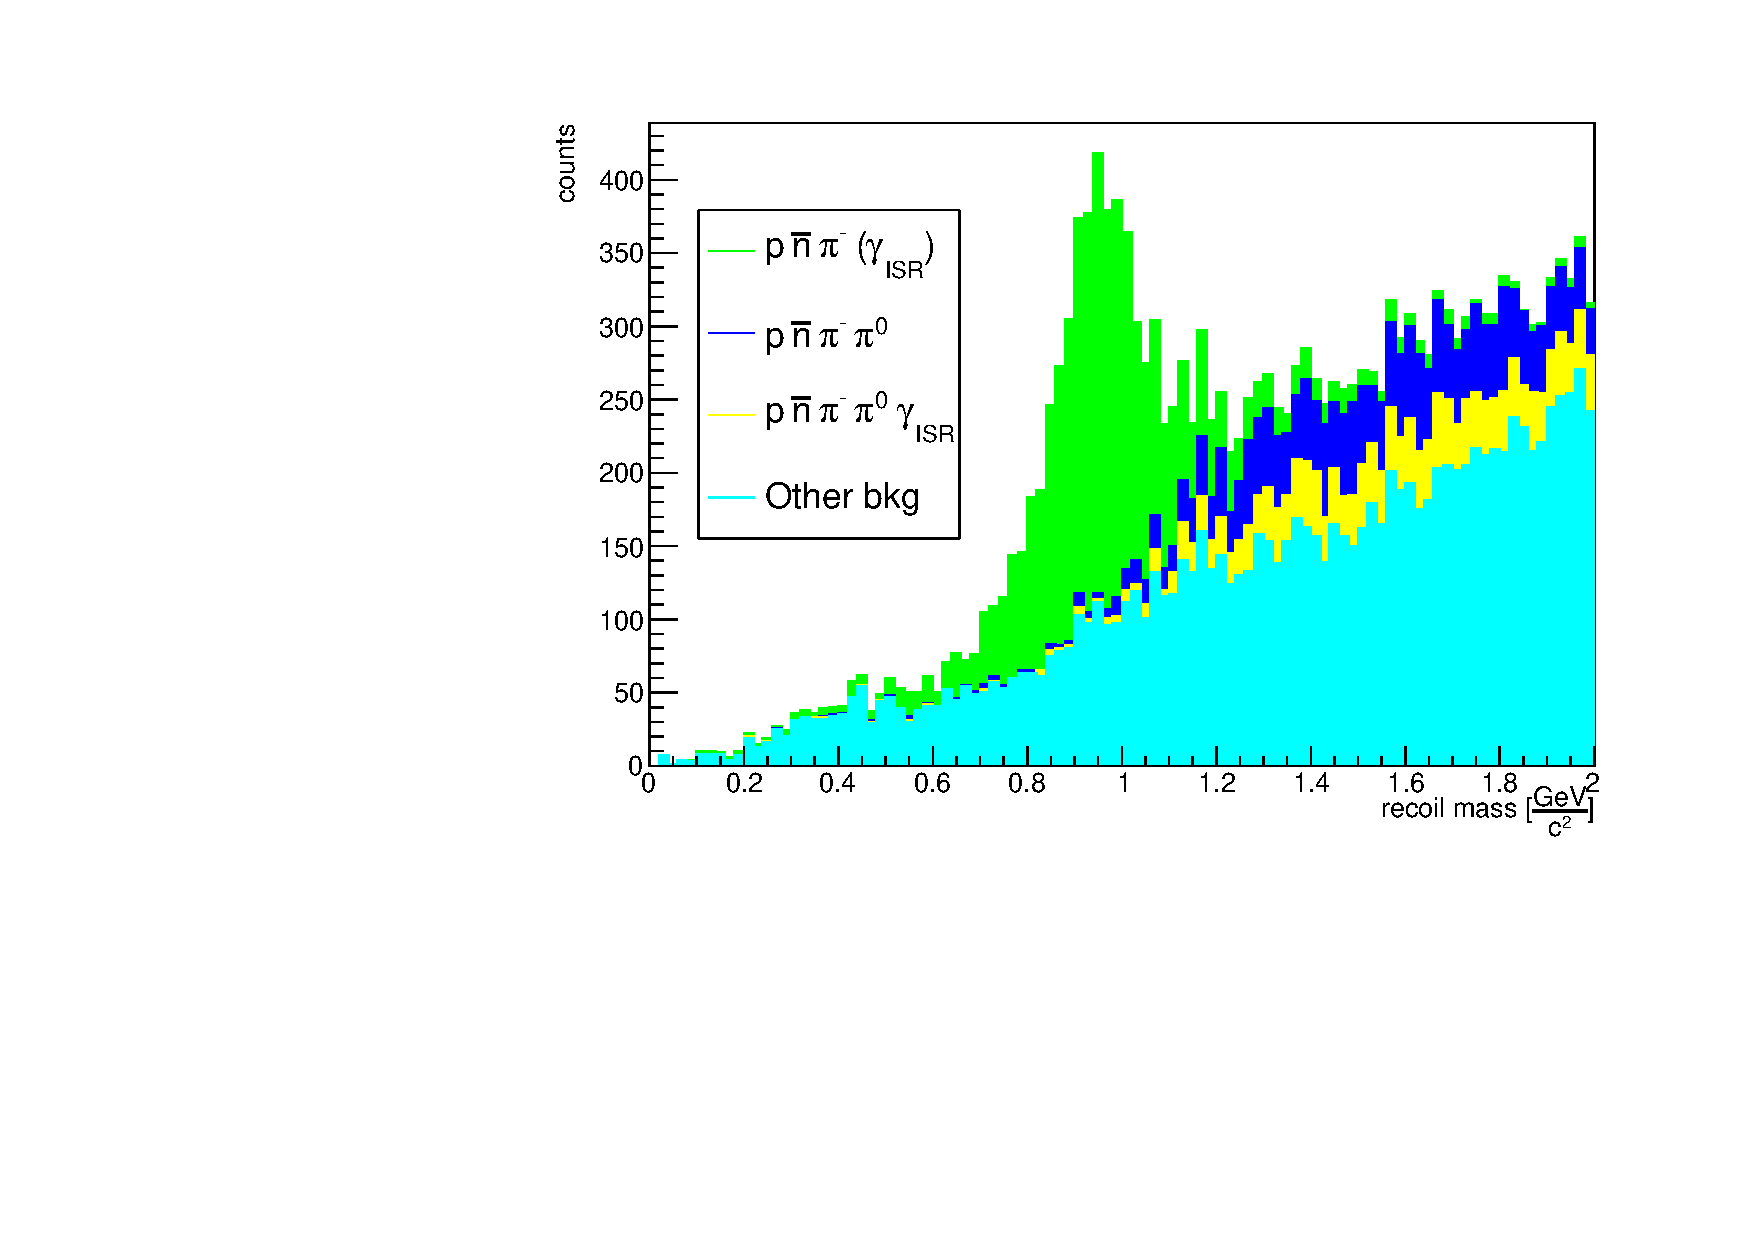
\includegraphics[width=0.90\textwidth]{nbar_cocktail/images/recoilM_comps_nog_020_0+3}
    \caption{$p, \pi^-$ recoil mass distribution in $u\bar{u}$ Monte Carlo cocktail, displaying each stacked component contribution, NO ISR case. Green: $\pi^- \bar{n} p$ and $\pi^- \bar{n} p \gamma_{ISR}$ channels. Blue: $\pi^0 \pi^- \bar{n} p$ channel. Yellow: $\pi^0 \pi^- \bar{n} p \gamma_{ISR}$ channel. Cyan: other channels.}
    \label{fig:mRecComps_nog_020_0+3}
\end{figure}
$\\$
To further suppress the background, a tighter $\alpha$ cut can be studied. Therefore, the Performance Metrics and their usage are investigated to find the most appropriate cut in $\alpha$.

\subsubsection{Performance Metrics study on $\alpha$ cut}
In general, a \textbf{Performance Metric} quantifies how a classification process is optimized based on a specific parameter, which could, for example, be represented by a threshold.
$\\$
In this specific HEP context, a performance metric quantifies how well the selection cuts distinguish the signal from the background. In this analysis, the signal can be assumed to be the channel with  $\pi^- \bar{n} p (\gamma_{ISR})$ in the final state, while the background is represented by all the other channels. Therefore, a stricter cut on the $\alpha$ angle is investigated to determine whether it improves signal selection over background.
$\\$
To address this kind of analysis, performance metrics such as the \textbf{Figure of Merit} (FOM), the Signal Efficiency ($\epsilon_{sig}$), the Background Efficiency ($\epsilon_{bkg}$) and the \textbf{purity} can be employed. These are defined as follow:
\begin{itemize}
\item FOM = $\frac{SIGNAL(\alpha)}{\sqrt{SIGNAL(\alpha) + BACKGROUND(\alpha)}}$;
\item $ \epsilon_{sig}  = \frac{SIGNAL(\alpha)}{SIGNAL(\alpha = 0.20 \ rad)}$;
\item $ \epsilon_{bkg}  =  \frac{BACKGROUND(\alpha)}{BACKGROUND(\alpha = 0.20 \ rad)}$;
\item Purity $= \frac{SIGNAL(\alpha)}{SIGNAL (\alpha)+ BACKGROUND(\alpha)}$.
\end{itemize}
SIGNAL and BACKGROUND are defined as follows:
\begin{itemize}
 \item SIGNAL($\alpha$) is defined by the number of entries from the signal channel, depending on $\alpha$;
 \item BACKGROUND($\alpha$) is defined by the number of entries from the other channels within the signal region, depending on $\alpha$.
 \end{itemize}
SIGNAL($\alpha$) + BACKGROUND ($\alpha$) = TOTAL($\alpha$), the total  amount of entries.
$\\$
Assuming the signal region corresponds to the interval $[0.8, 1.2]$ GeV, the FOM characterizes the statistical significance of the applied threshold, namely the selected cut on $\alpha$. The higher the FOM, the more signal is selected over the background (the figure is maximized). For each possible cut value of $\alpha$, the Figure of Merit (FOM) is computed and the cut corresponding to the maximum FOM (or to a stable plateau) is selected. A higher FOM indicates a better trade-off between signal efficiency and background rejection, so the selection is optimized when the FOM is maximized. The obtained FOM is shown in Fig.~\ref{fig:fom_alpha020}.
\begin{figure}[h]
    \centering
    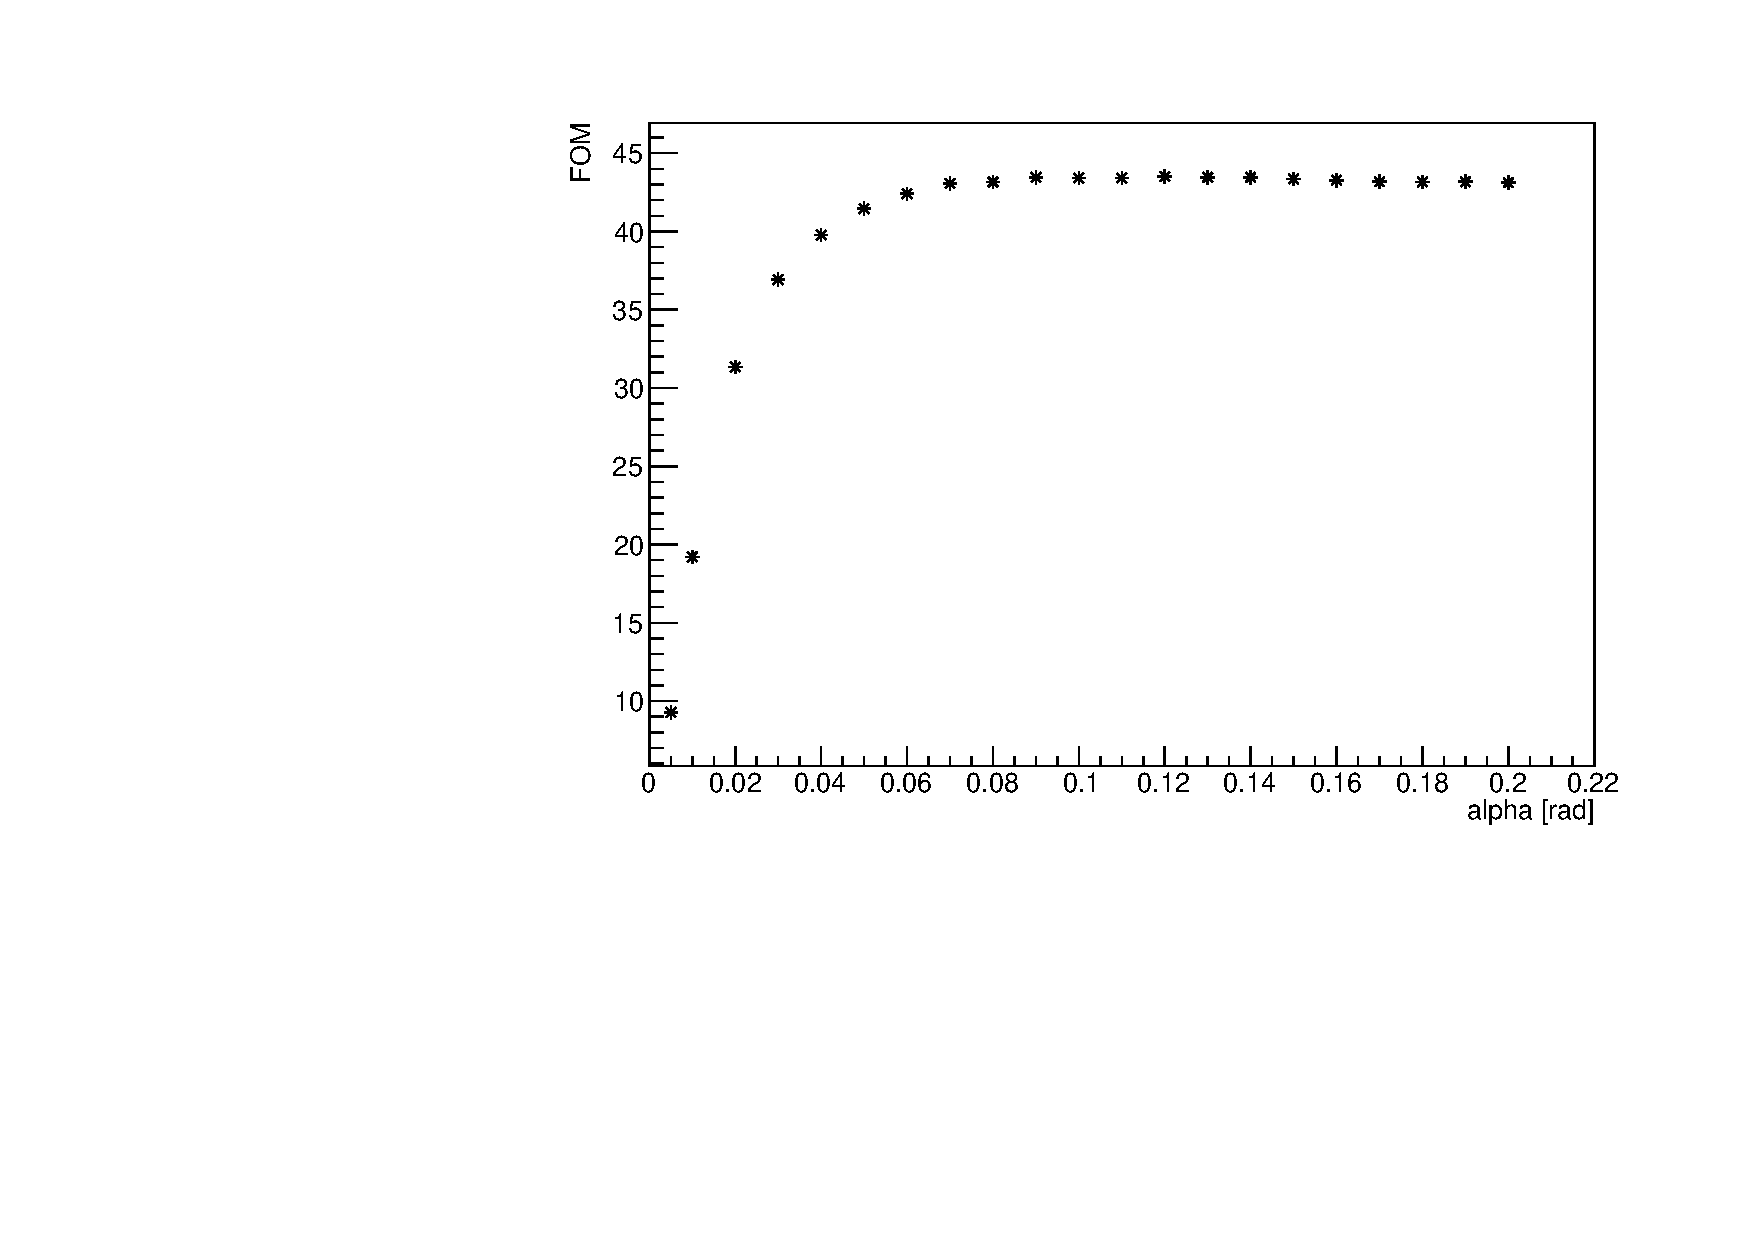
\includegraphics[width=0.70\textwidth]{nbar_cocktail/images/fom_alpha}
    \caption{Figure of Merit (FOM) versus $\alpha$ angle for the $u\bar{u}$ cocktail.}
    \label{fig:fom_alpha020}
\end{figure}
$\\$
One $\alpha$ value corresponding to the plateau can be chosen in order to maximize the FOM. The value $\alpha < 0.1$ rad ($\sim 5.73^\circ$) is therefore chosen, corresponding to FOM = 43.4185
$\\$
Furthermore, the signal efficiency $\epsilon_{sig}$ and the background efficiency $\epsilon_{bkg}$ performance metrics can be adopted to study the Receiver Operating Characteristic (ROC), a curve that shows how well a binary classifier distinguishes signal from background as the decision threshold ($\alpha$ cut) is varied.
Each point on the curve corresponds to a different threshold (a cut on the $\alpha$ angle). The Area Under the ROC Curve (AUC/ROC-AUC) is a single number summarizing the overall performance: 1.0 indicates perfect discrimination, while 0.5 corresponds to no better performance than random. The obtained ROC is shown in Fig.~\ref{fig:roc_alpha020}.
\begin{figure}[H]
    \centering
    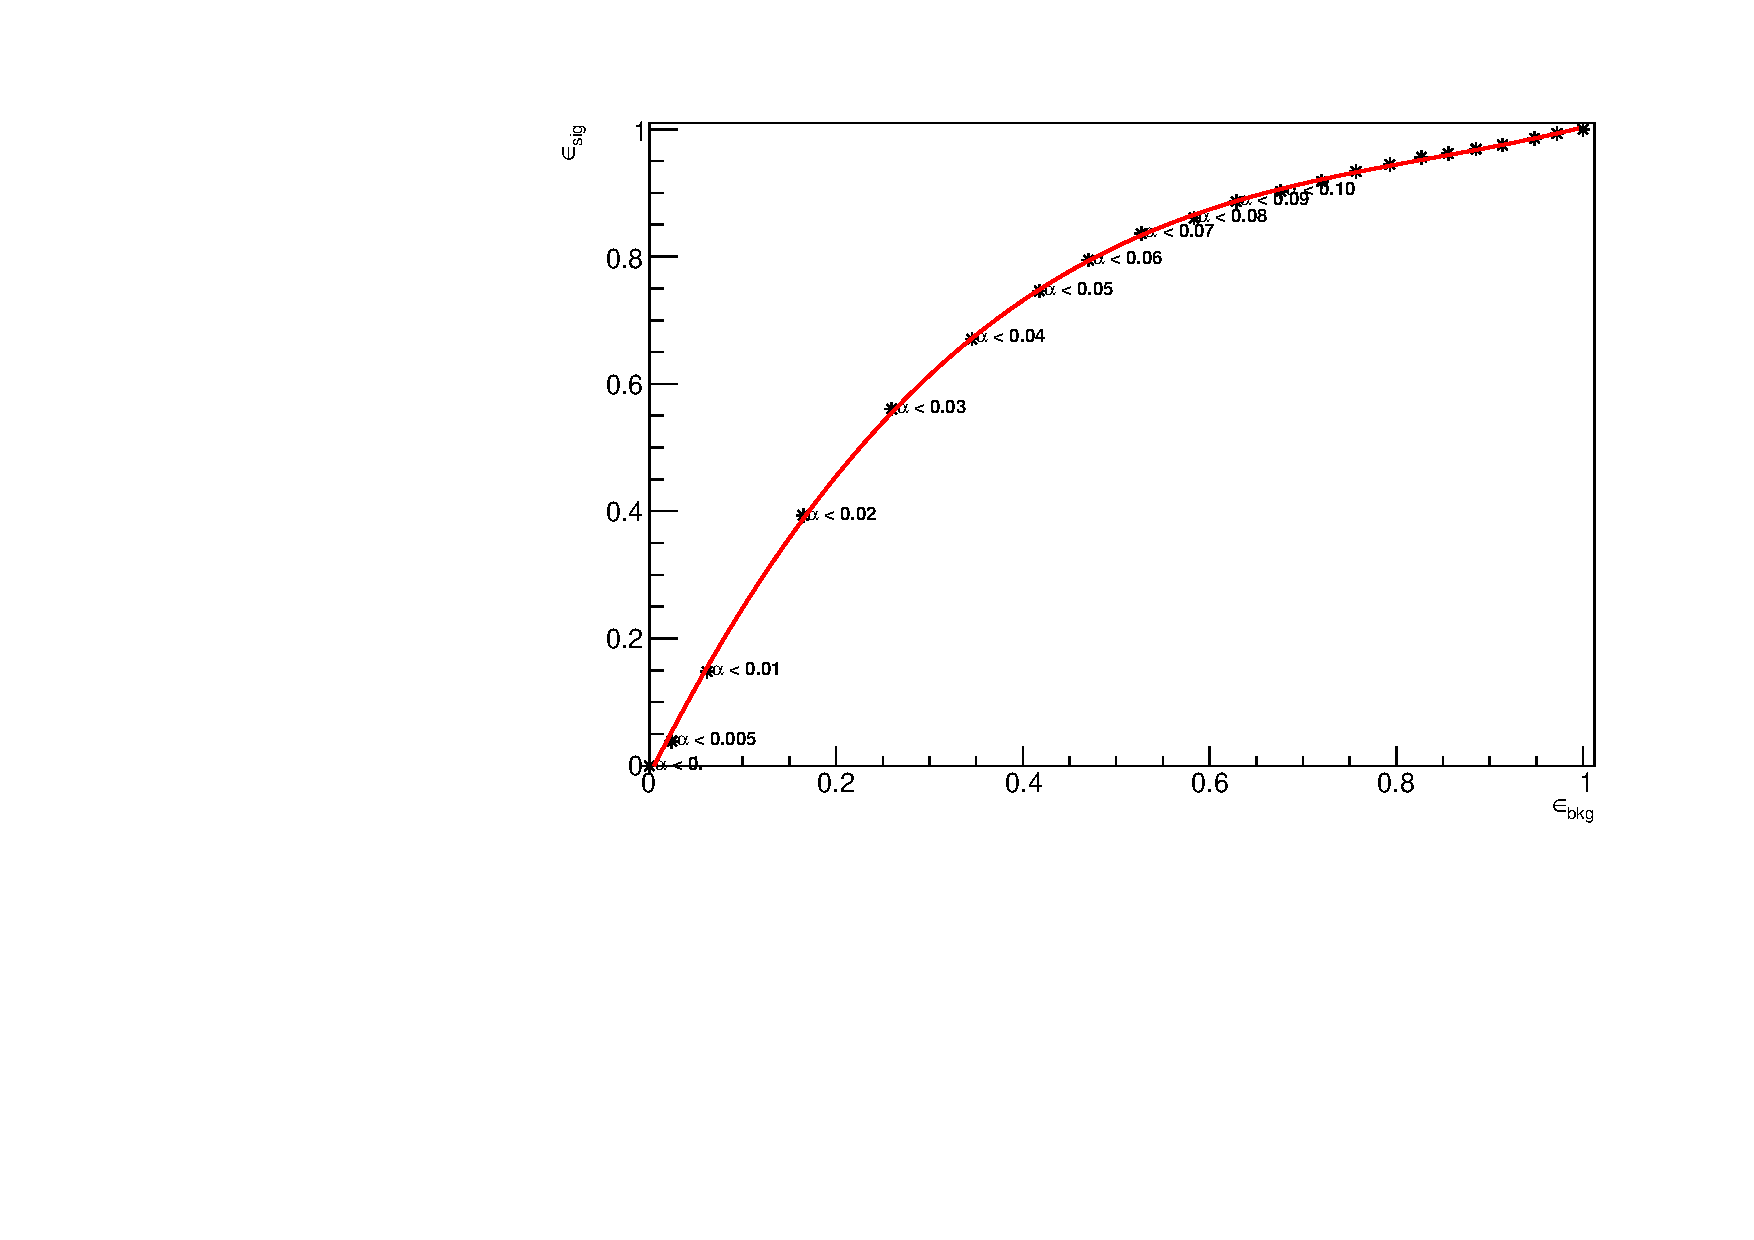
\includegraphics[width=0.70\textwidth]{nbar_cocktail/images/roc_alpha_true}
    \caption{Receiver Operating Characteristic (ROC) curve constructed from the signal efficiency ($\epsilon_{sig}$) and the Background Efficiency ($\epsilon_{bkg}$), where each point corresponds to a different cut value on the $\alpha$ angle. The labels are shown only for $\alpha < 0.10$ rad.}
    \label{fig:roc_alpha020}
\end{figure}

The Receiver Operating Characteristic (ROC) curve for the $\alpha$ angle cut yields an area under the curve (AUC) of $0.71$, indicating good discrimination power between signal and background.
$\\$
Therefore, the obtained performance metrics for $\alpha < 0.1$ rad are:
\begin{center}
$FOM = 43.4185$, $\epsilon_{sig}= 90\%$, $\epsilon_{bkg}= 68\%$,  $Purity = 63\%$
\end{center}
The obtained $\epsilon_{sig}$ vs $Purity$ is shown in Fig.~\ref{fig:eff_alpha020}.
\begin{figure}[H]
    \centering
    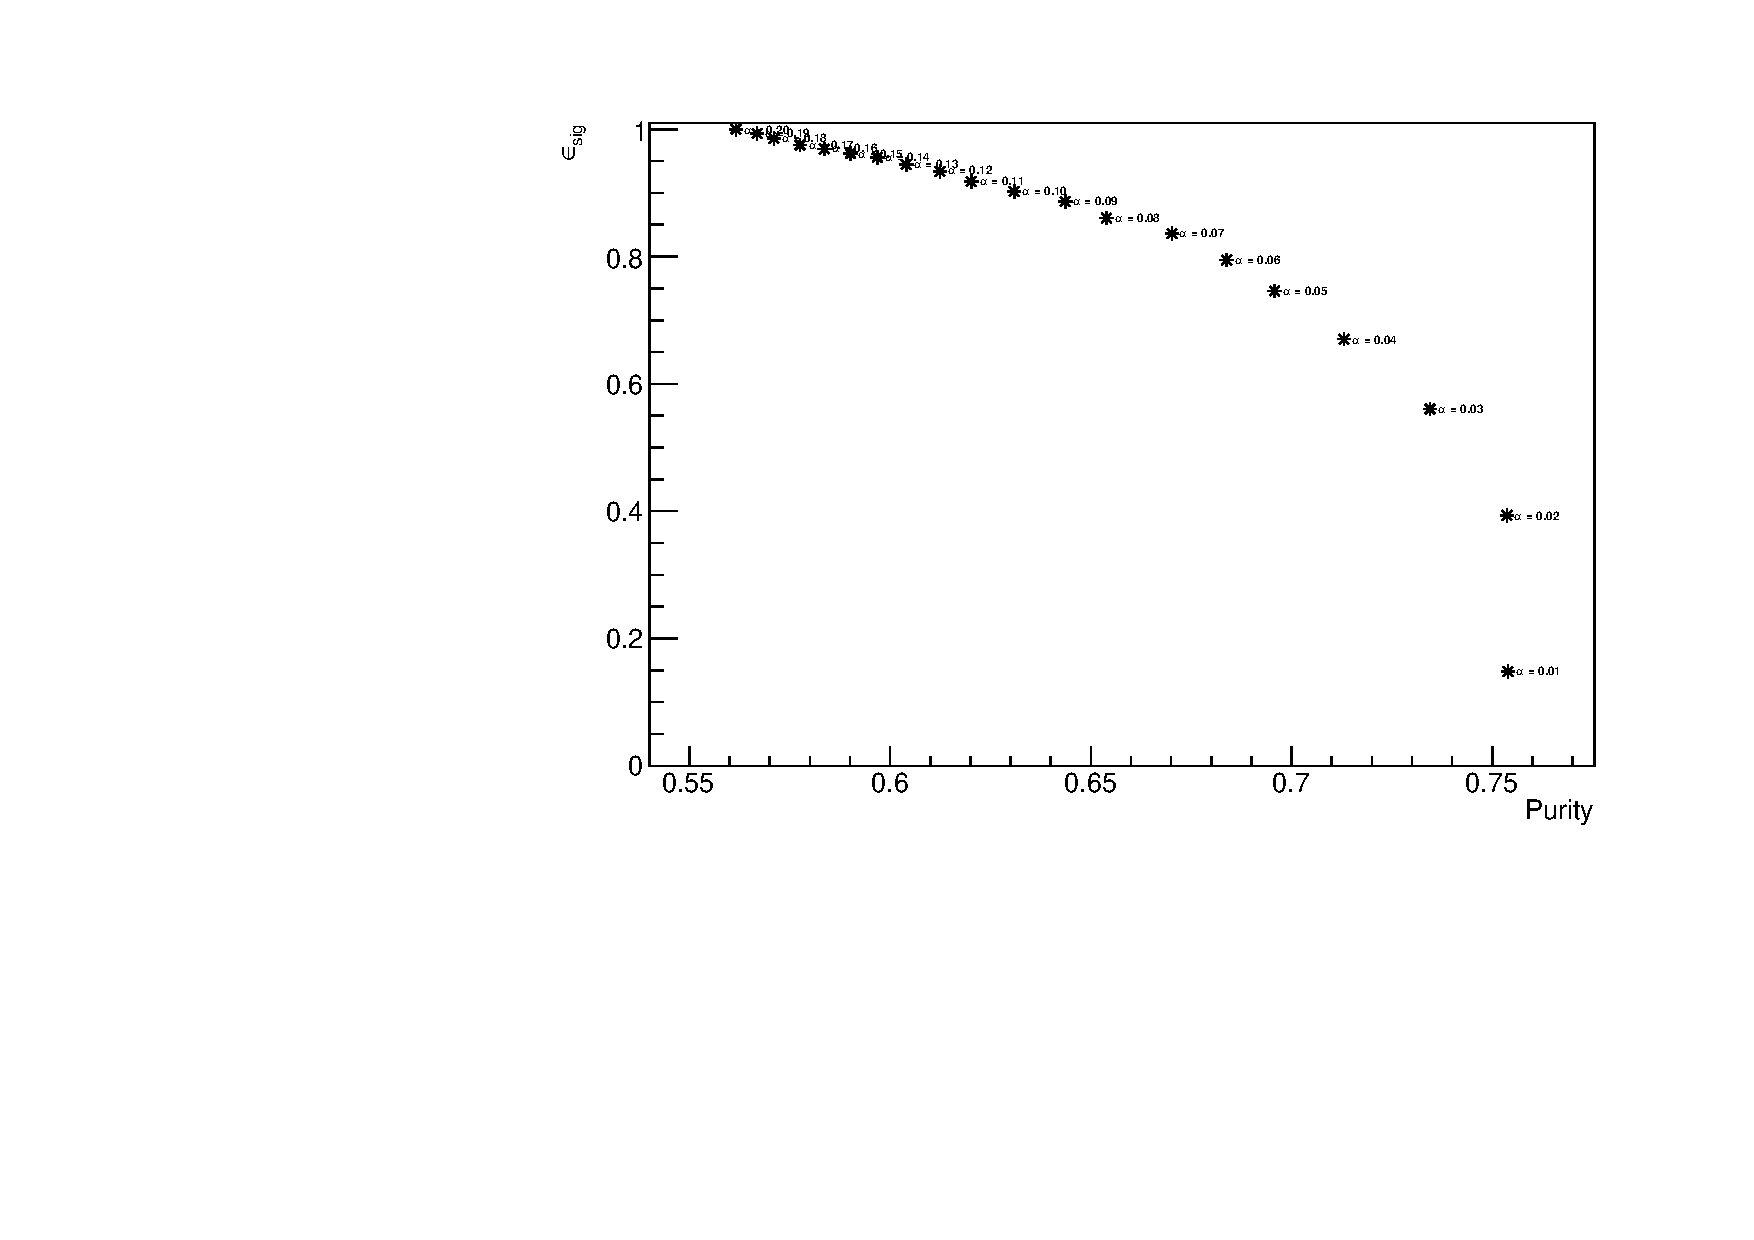
\includegraphics[width=0.70\textwidth]{nbar_cocktail/images/eff_alpha}
    \caption{ $\epsilon_{sig}$ vs $Purity$ curve for the $u\bar{u}$ Monte Carlo cocktail.}
    \label{fig:eff_alpha020}
\end{figure}
Following the described optimization, the recoil mass channel components distribution can now be analyzed using the cut $\alpha < 0.10$ rad.
$\\$
The obtained stacked component to the recoil mass are shown in Fig.~\ref{fig:mRecComps_nog_010}.
\begin{figure}[h]
    \centering
    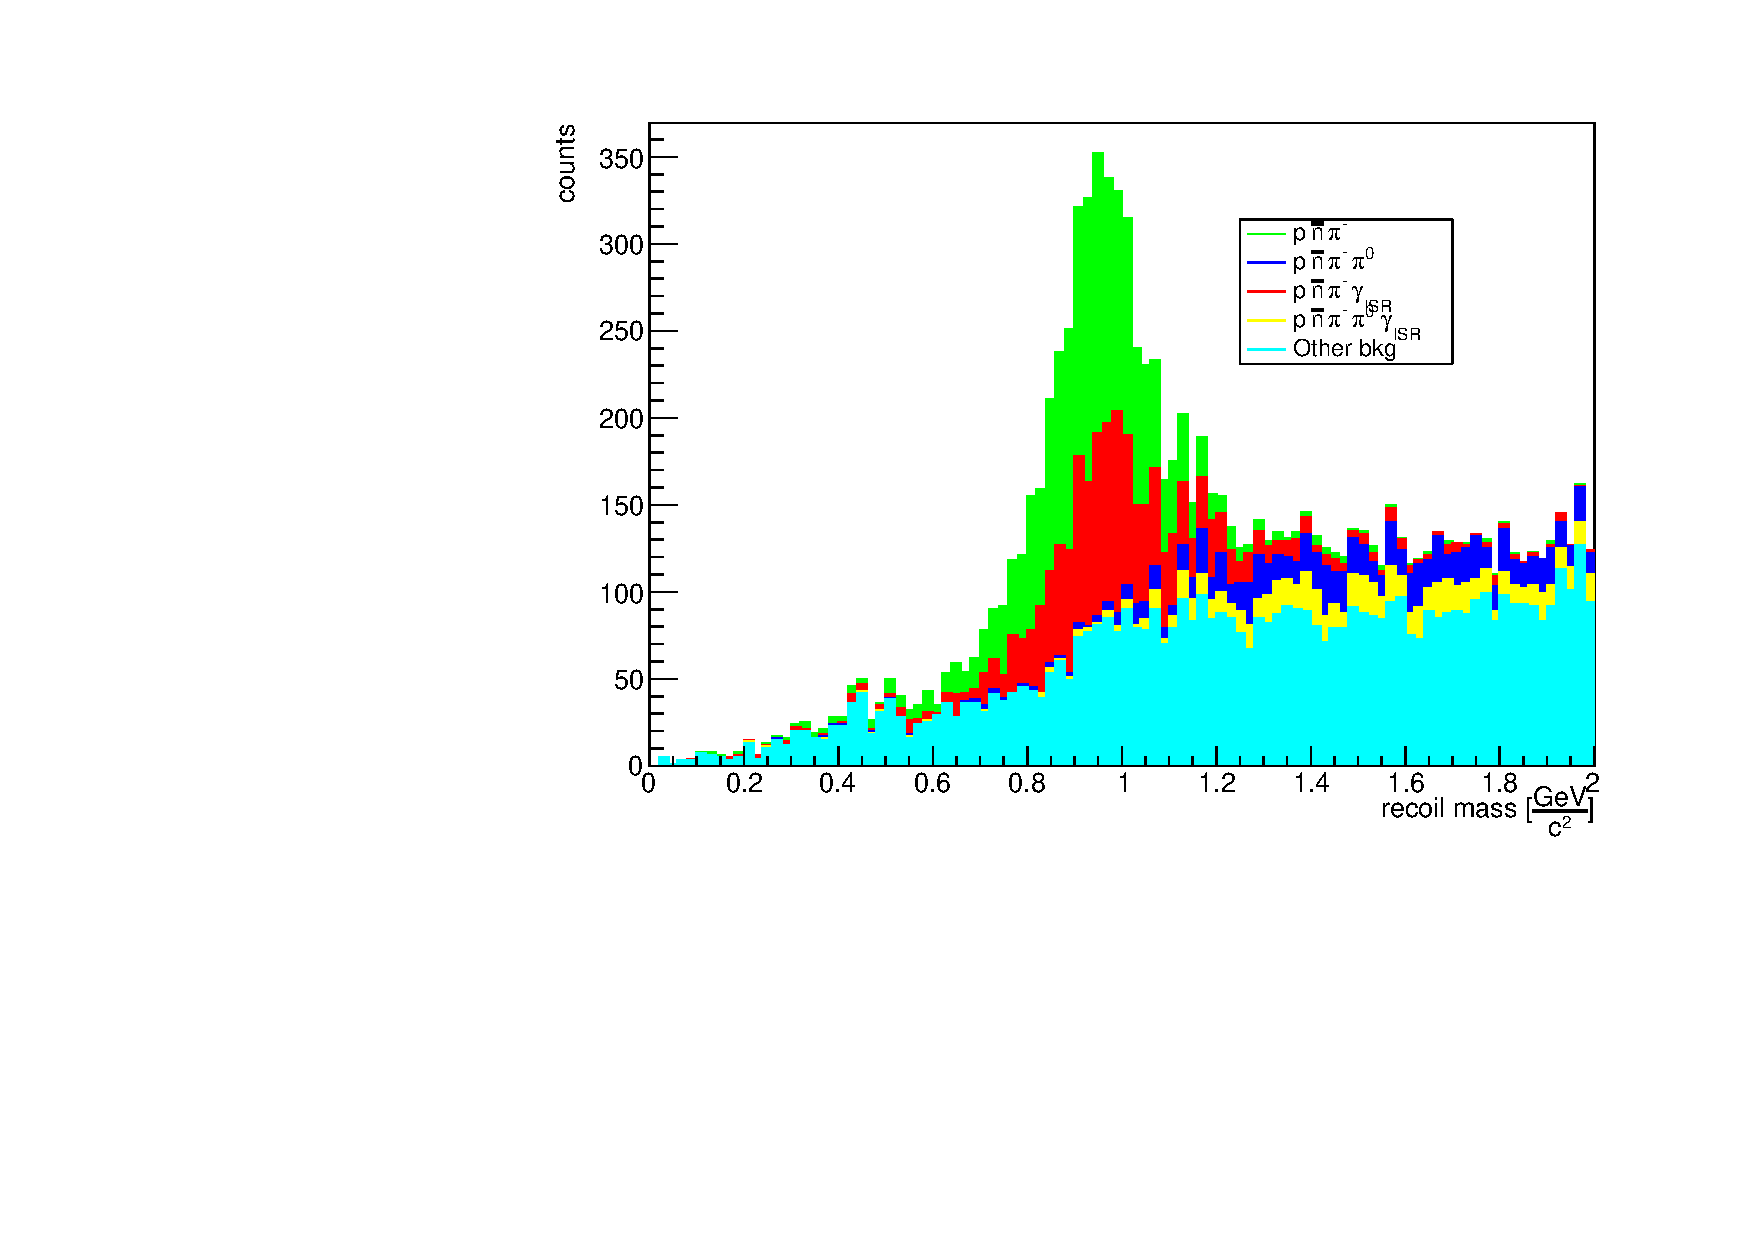
\includegraphics[width=0.8\textwidth]{nbar_cocktail/images/recoilM_comps_nog_010}
    \caption{$p, \pi^-$ recoil mass distribution, displaying each stacked component contribution, NO ISR case. Green: $\pi^- \bar{n} p$ channel. Blue: $\pi^0 \pi^- \bar{n} p$ channel. Red: $\pi^- \bar{n} p \gamma_{ISR}$. Yellow: $\pi^0 \pi^- \bar{n} p \gamma_{ISR}$ channel. Cyan: other channels. $\alpha<$ 10 rad cut is applied.}
    \label{fig:mRecComps_nog_010}
\end{figure}

As observed in the performance metrics study, the signal is more prominent relative to the background than in the previous case. Background components containing $\pi^0$ peak outside the signal region $[0.8,1.2]$ GeV on the right side, while other sources exhibit a lower, flat distribution across the recoil mass spectrum.
$\\$
The first 5 channels of $u\bar{u}$ TopoAna output with the $\alpha<$ 10 rad cut is shown in ~\ref{fig:topo_nog_010_uubar}.
\begin{figure}[h]
    \centering
    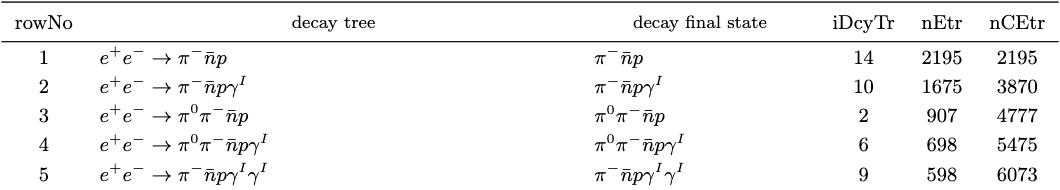
\includegraphics[width=1\textwidth]{nbar_cocktail/images/topo_uubar_010}
    \caption{Top 5 channels from the TopoAna output for the $u\bar{u}$ Monte Carlo cocktail. NO ISR case.}
    \label{fig:topo_nog_010_uubar}
\end{figure}

After applying the $\alpha < 0.10$ rad cut, the dominant contribution remains from the signal channel $p \pi^- \bar{n}$, now immediately followed by $p \pi^- \bar{n} \gamma_{\text{ISR}}$. Both contributions can be identified as signal since they fall within the signal region $[0.8,1.2]$ GeV.

\subsection{$q\bar{q}$ cocktail production (NO ISR case)}
In order to fully characterize the Monte Carlo simulation, all $q\bar{q}$ continuum components are studied. The Run 1 Monte Carlo productions for $u\bar{u}$, $d\bar{d}$, $s\bar{s}$, and $c\bar{c}$ are therefore analyzed.
$\\$
For a cleaner comparison between the signal channel and background components, the TopoAna output can be consulted in Fig.~\ref{fig:topo_nog_010_qqbar}.
\begin{figure}[H]
    \centering
    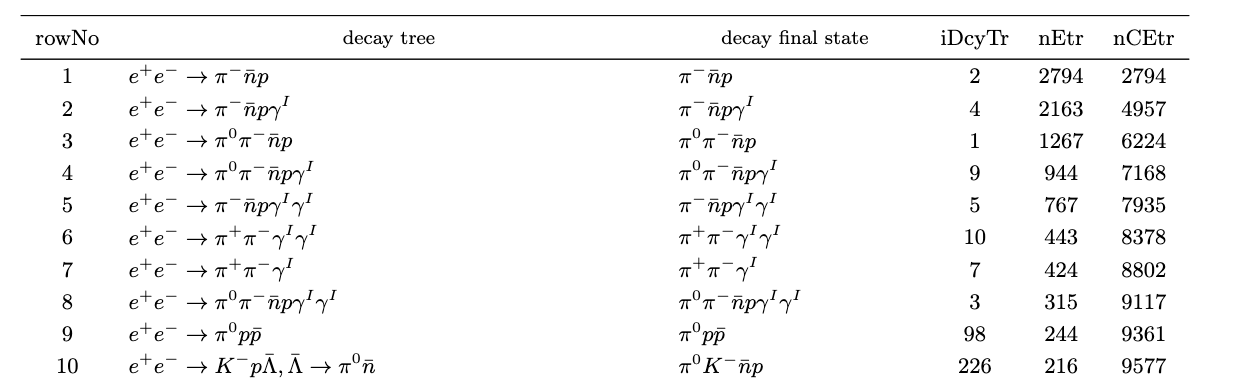
\includegraphics[width=1\textwidth]{nbar_cocktail/images/topoana_nog_010_qqbar}
    \caption{First 10 channels of the TopoAna output in $q\bar{q}$ Monte Carlo cocktail, showing the different channel contributes.}
    \label{fig:topo_nog_010_qqbar}
\end{figure}
The TopoAna output reveals that the dominant contribution is from the signal channel $p \pi^- \bar{n}$ in the $q\bar{q}$ continuum. A secondary contribution comes from $p \pi^- \bar{n} \gamma_{ISR}$, which could be treated as signal despite the $\gamma_{\text{ISR}}$ not being explicitly reconstructed. The next contribution comes from $p \pi^- \bar{n} \pi^0$ in the final state. The fourth contribution is due to $p \pi^- \bar{n} \pi^0 \gamma_{\text{ISR}}$, and so on. The situation is very similar to that observed in the $u\bar{u}$ case.
$\\$
The individual TopoAna outputs separately for the $u\bar{u}$, $d\bar{d}$, $s\bar{s}$, and $c\bar{c}$ samples are now discussed. The first 5 contributes for each sample are shown in ~\ref{fig:topo_nog_010_qqbar_singles}.
\begin{figure}[h]
    \centering
    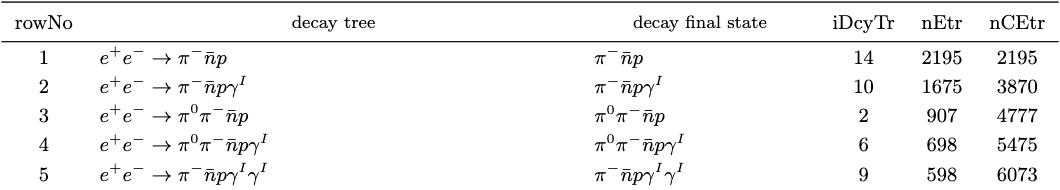
\includegraphics[width=1\textwidth]{nbar_cocktail/images/topo_uubar_010}
    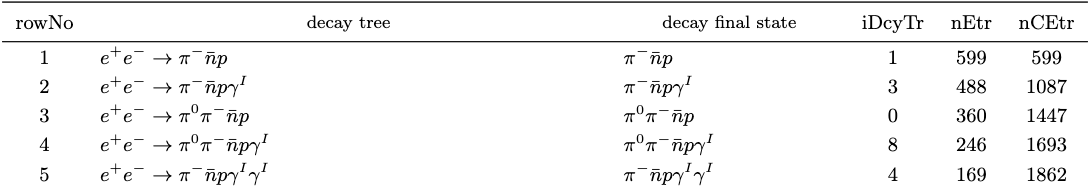
\includegraphics[width=1\textwidth]{nbar_cocktail/images/topo_ddbar_010}
    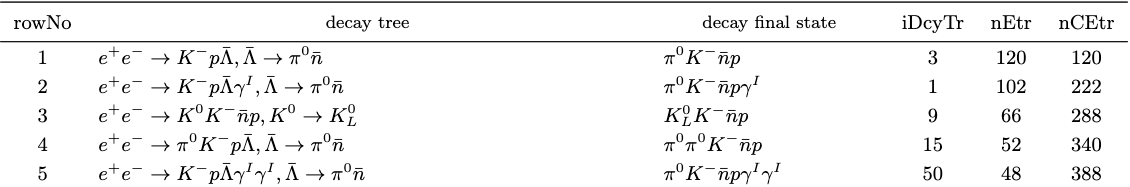
\includegraphics[width=1\textwidth]{nbar_cocktail/images/topo_ssbar_010}
    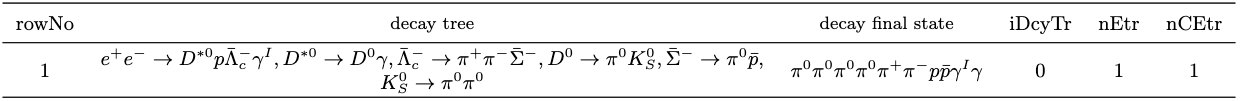
\includegraphics[width=1\textwidth]{nbar_cocktail/images/topo_ccbar_010}
    \caption{Top 5 channels from the TopoAna output respectively for the $u\bar{u}$, $d\bar{d}$, $s\bar{s}$, and $c\bar{c}$ Monte Carlo cocktails (from top to bottom). NO ISR case. The \texttt{iDcyTr} index values may differ across samples, since each TopoAna output is produced independently from its corresponding ROOT ntuples.}
    \label{fig:topo_nog_010_qqbar_singles}
\end{figure}
The main contributions to the final signal state are from the $u\bar{u}$ and $d\bar{d}$ cocktails, as expected, since no $p\pi^-\bar{n}$ system can be obtained from an $s\bar{s}$ state. A contribution from a $c\bar{c}$ state could have been expected from the following channel:

\begin{center}
$e- \ + \ e^- \rightarrow J/\Psi (c\bar{c}) \rightarrow p \ + \ \pi^- \ + \ \bar{n}$
\end{center}
In order to reach the $J/\psi$ resonance ($\sim 3.1$ GeV) in $e^+e^-$ collisions at Belle II, a significant lowering of the center-of-mass energy must occur due to $\gamma_{\rm ISR}$ emission. Since high-energy ISR emission is improbable (Fig.~\ref{fig:isr_distro}), the $c\bar{c}$ channel can be considered negligible for this analysis.
$\\$
The obtained stacked components to the recoil mass, in $q\bar{q}$ cocktail, are shown in figure ~\ref{fig:mRecComps_nog_010_qqbar}.
\begin{figure}[H]
    \centering
    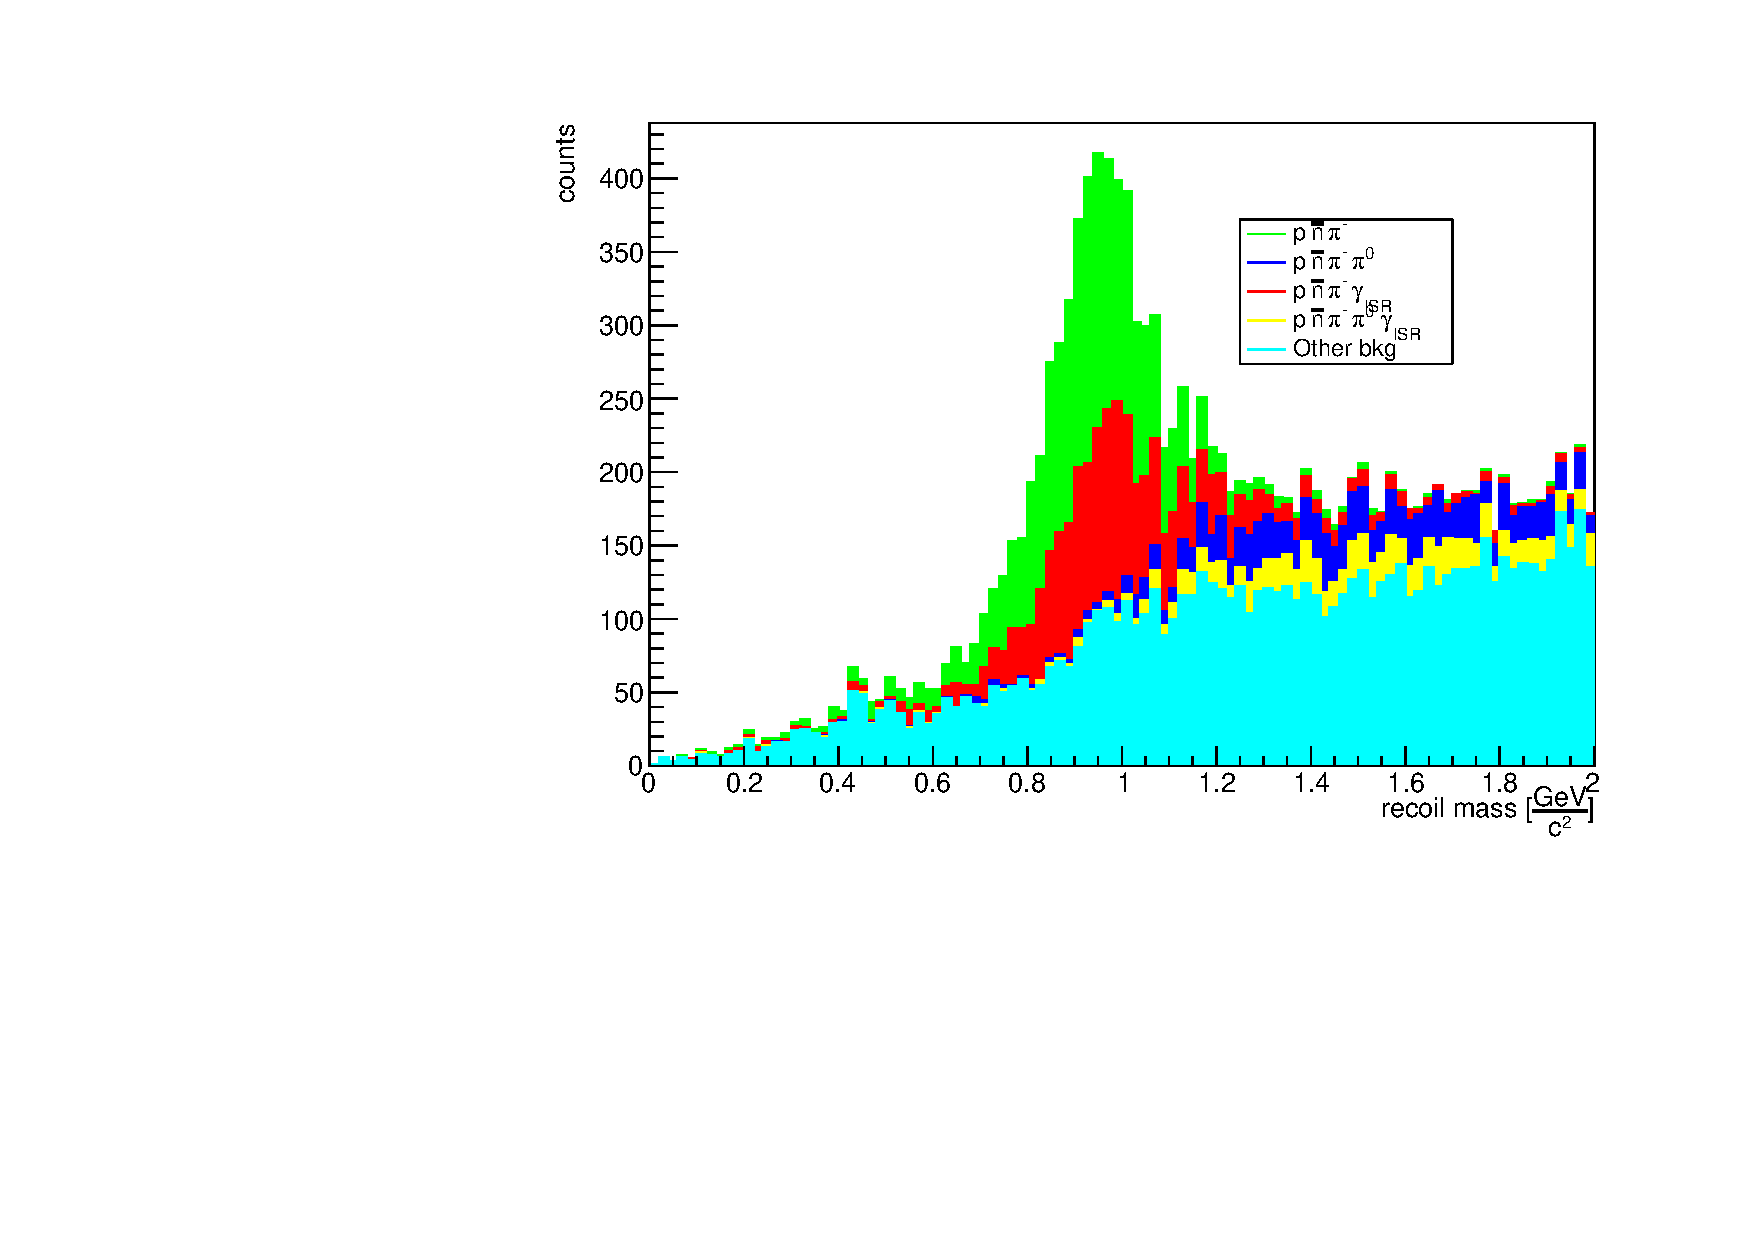
\includegraphics[width=0.8\textwidth]{nbar_cocktail/images/recoilM_qqbar_comps_nog_010}
    \caption{$p, \pi^-$ recoil mass distribution in $q\bar{q}$ Monte Carlo cocktail, displaying each stacked component contribution, NO ISR case. Green: $\pi^- \bar{n} p$ channel. Blue: $\pi^0 \pi^- \bar{n} p$ channel. Red: $\pi^- \bar{n} p \gamma_{ISR}$. Yellow: $\pi^0 \pi^- \bar{n} p \gamma_{ISR}$ channel. Cyan: other channels. $\alpha<$ 10 rad cut is applied.}
    \label{fig:mRecComps_nog_010_qqbar}
\end{figure}
A similar behaviour to the $u\bar{u}$ cocktail can be observed, where the $p\pi^-\bar{n}$ and $p\pi^-\bar{n}\gamma_{\text{ISR}}$ channels mainly contribute to the signal region [0.8,1.2] GeV. Background components containing the $\pi^0$ peak appear outside the signal region [0.8,1.2] GeV on the right side, while a flat background is present from other background channels.

\subsubsection{Cluster variables in $q\bar{q}$ cocktail}
The $\bar{n}$ candidates reconstructed cluster variables can now be studied with the following discussed selections:
\begin{enumerate}
\item Recoil system: $0 \ GeV/c^2 <recoil \ mass < 2 \ GeV/c^2$ and in ECL acceptance;
\item $\bar{n}$: neutral clusters from ECL and number of hits $> 10$ and energy $<3$ GeV;
\item $p$: $protonID > 0.9$ and $dr<1$ cm and $|dz|<3$ cm;
\item $\pi^-$: $pionID > 0.1$ and $dr<1$ cm and $|dz|<3$ cm; 
\item $\alpha <0.10$ rad $\sim 5.73^\circ$;
\item No further charged particles in the Rest of Event (ROE).
\end{enumerate}
The obtained $\bar{n}$ candidates reconstructed cluster variables are shown in Fig.\ref{fig:clus_vars_nog_qqbar}.
Specific structures can be observed in the cluster variables distributions, compared to those obtained in Fig.~\ref{fig:clus_vars_2}.
$\\$
For example, in the E1E9 distribution a second structure can be noted at a value $\sim 0.85$, and at value $\sim 1$ in the E9E21distribution as well. Similar structure appears at values close to 0 in the Second Moment distribuiton, which is partially reflected in the first structure of the N Hits distribution observed at a value of $\sim 10$. Another example can be seen in the Lateral Momentum distribution, where a structure at $\sim 0.3$ can be noted, which is typical reference of electromagnetic shower. 
$\\$
Therefore, a contribution from small-sized clusters -as can be seen in the Second Moment and N Hits distributions- and not spread out clusters -as can be seen in the E1E9 and E9E21 distributions- can be observed in $\bar{n}$ candidates reconstructed cluster variables. These shower shape characteristics are typical of the electromagnetic showers. This is further suggested by the structure observed in the Lateral Momentum distribution.
$\\$
In order to study the nature of these singular structures, a signal and background study can be performed, isolating the individual contribution of each. If these structures are not produced by the signal, their contribution could be isolated and then removed from the signal one. In order to perform this kind of analysis, the sidebands technique is discussed in the next paragraph.

\newpage
The obtained cluster variables distribution in NO ISR case, in q$\bar{q}$ cocktail.
 \begin{figure}[H]
    \centering
    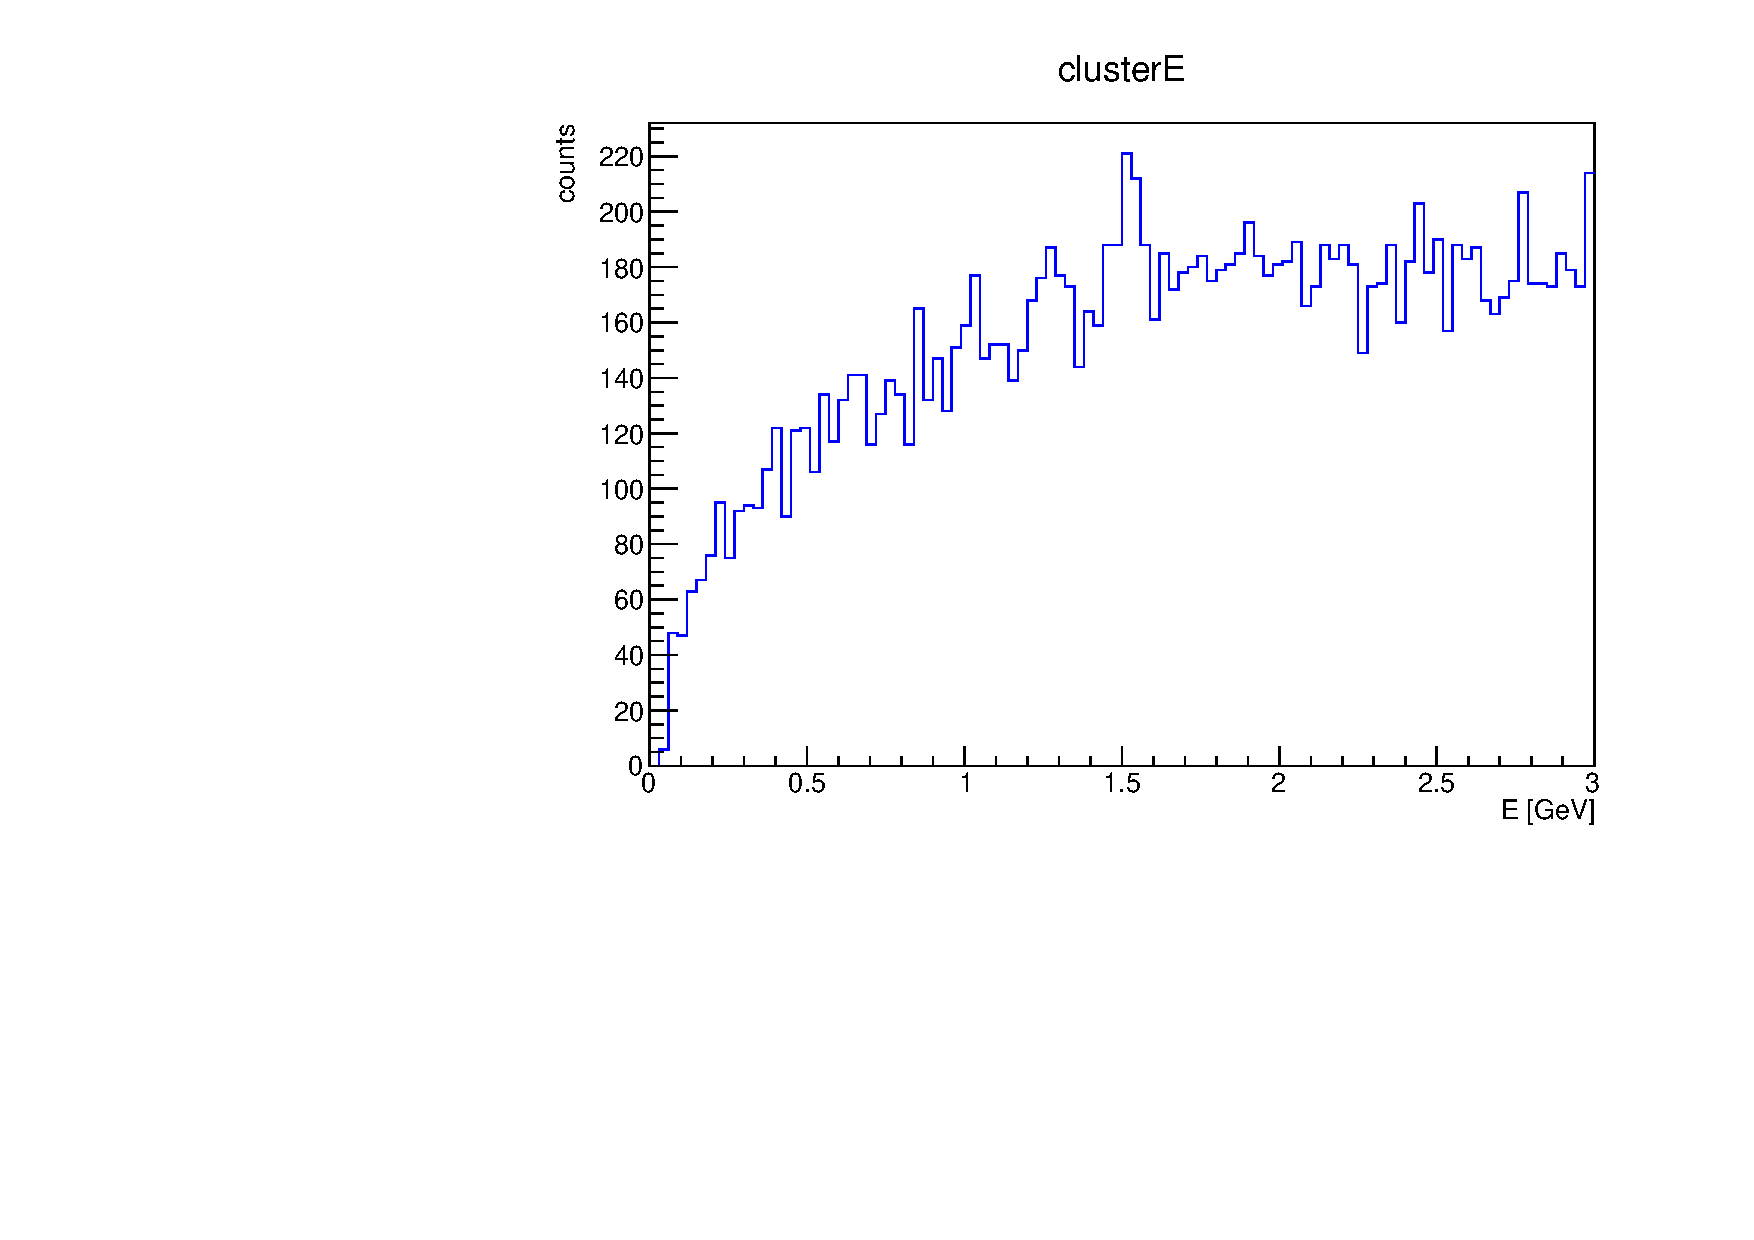
\includegraphics[width=0.49\textwidth]{nbar_cocktail/images/clusterE_nog_qqbar.pdf}
    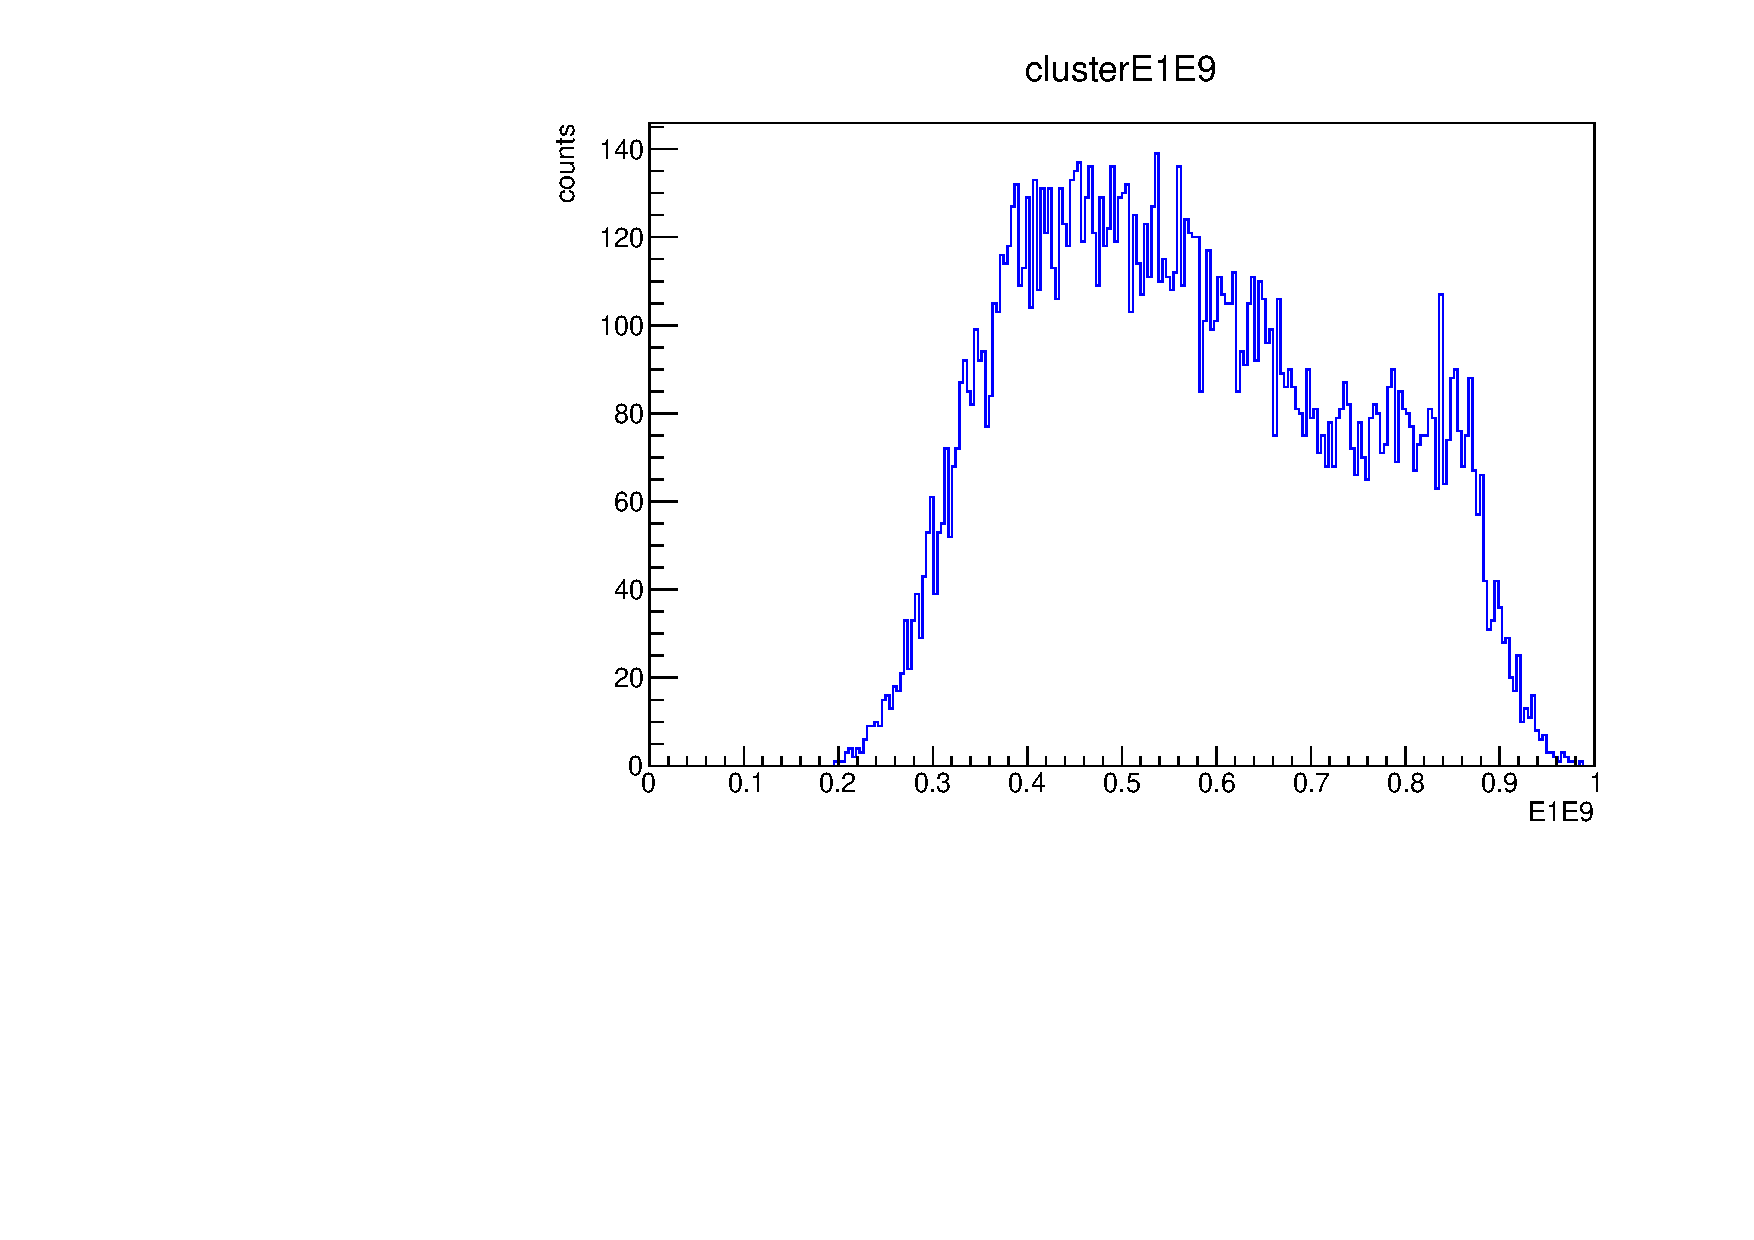
\includegraphics[width=0.49\textwidth]{nbar_cocktail/images/clusterE1E9_nog_qqbar.pdf}
    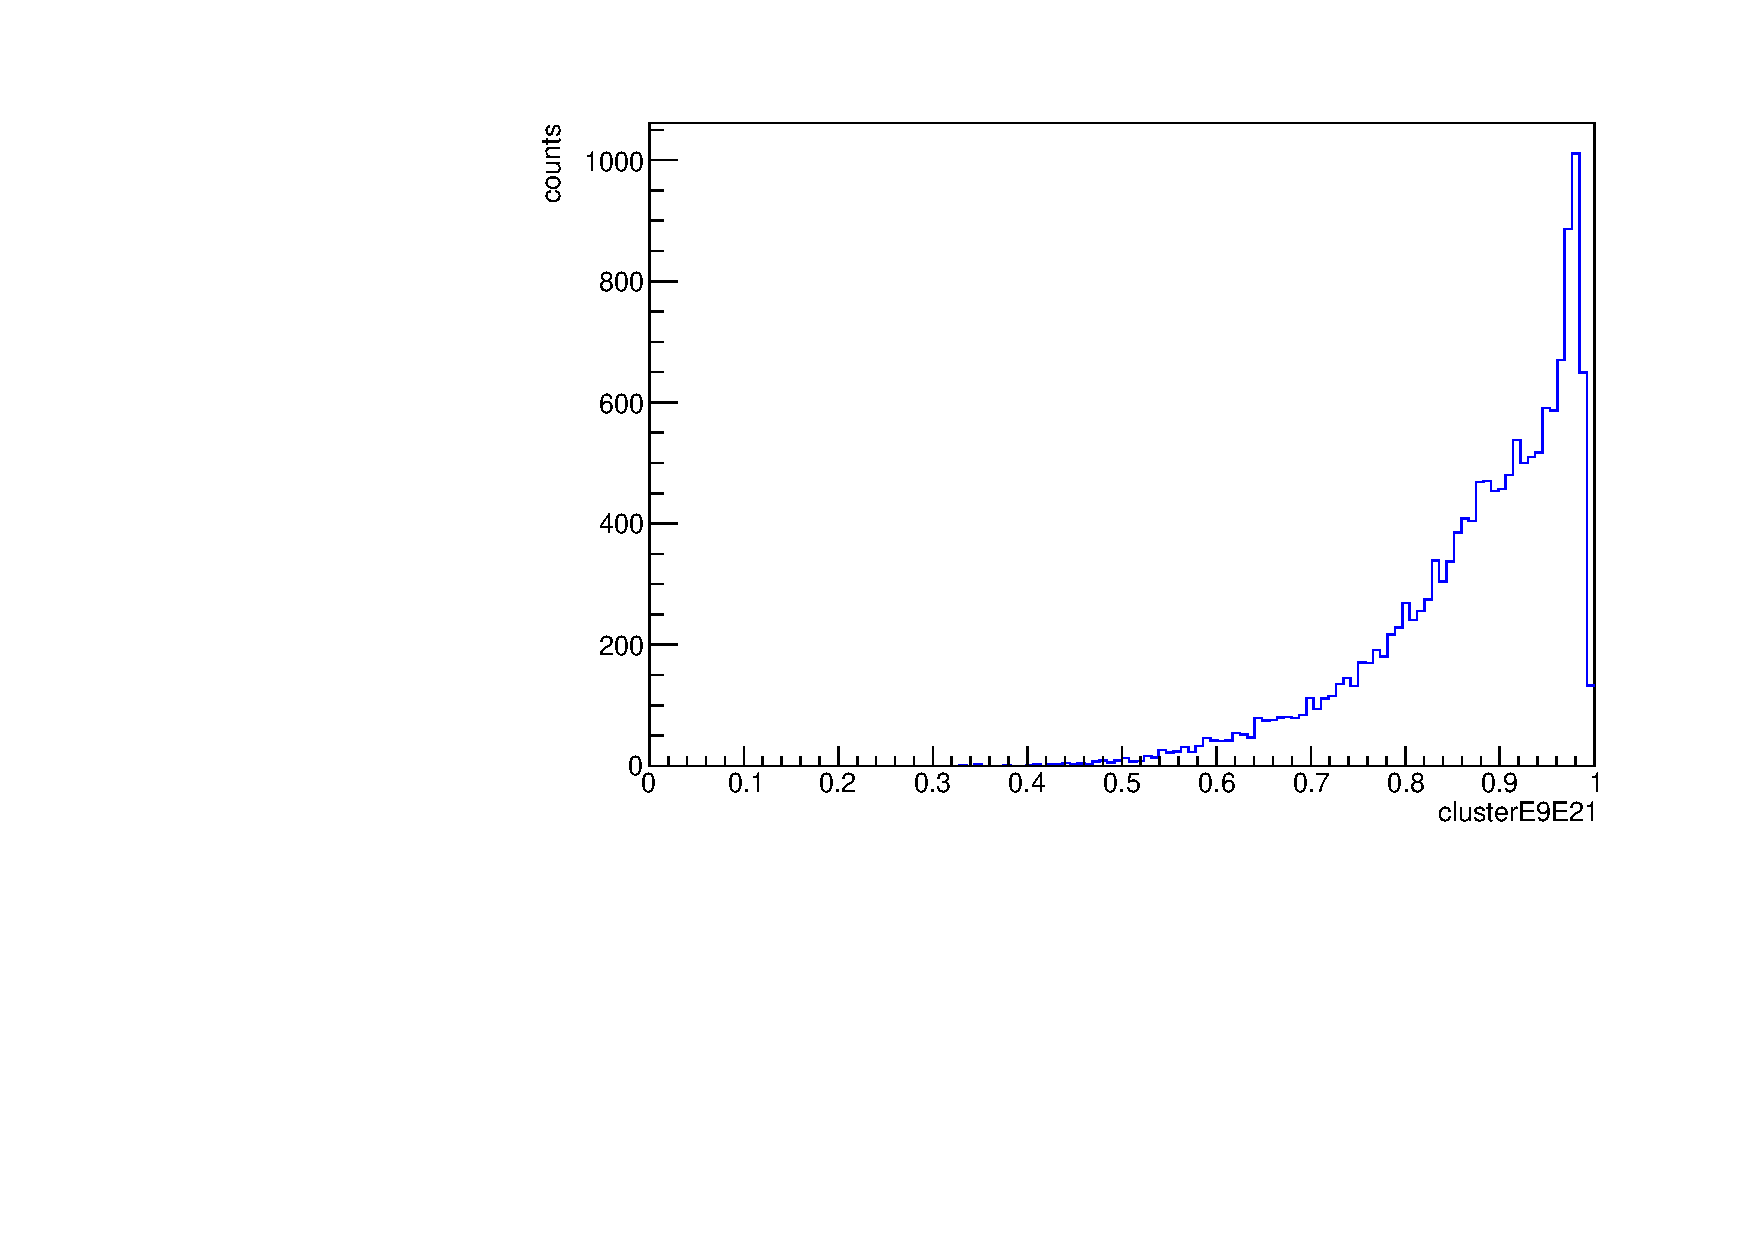
\includegraphics[width=0.49\textwidth]{nbar_cocktail/images/clusterE9E21_nog_qqbar.pdf}
    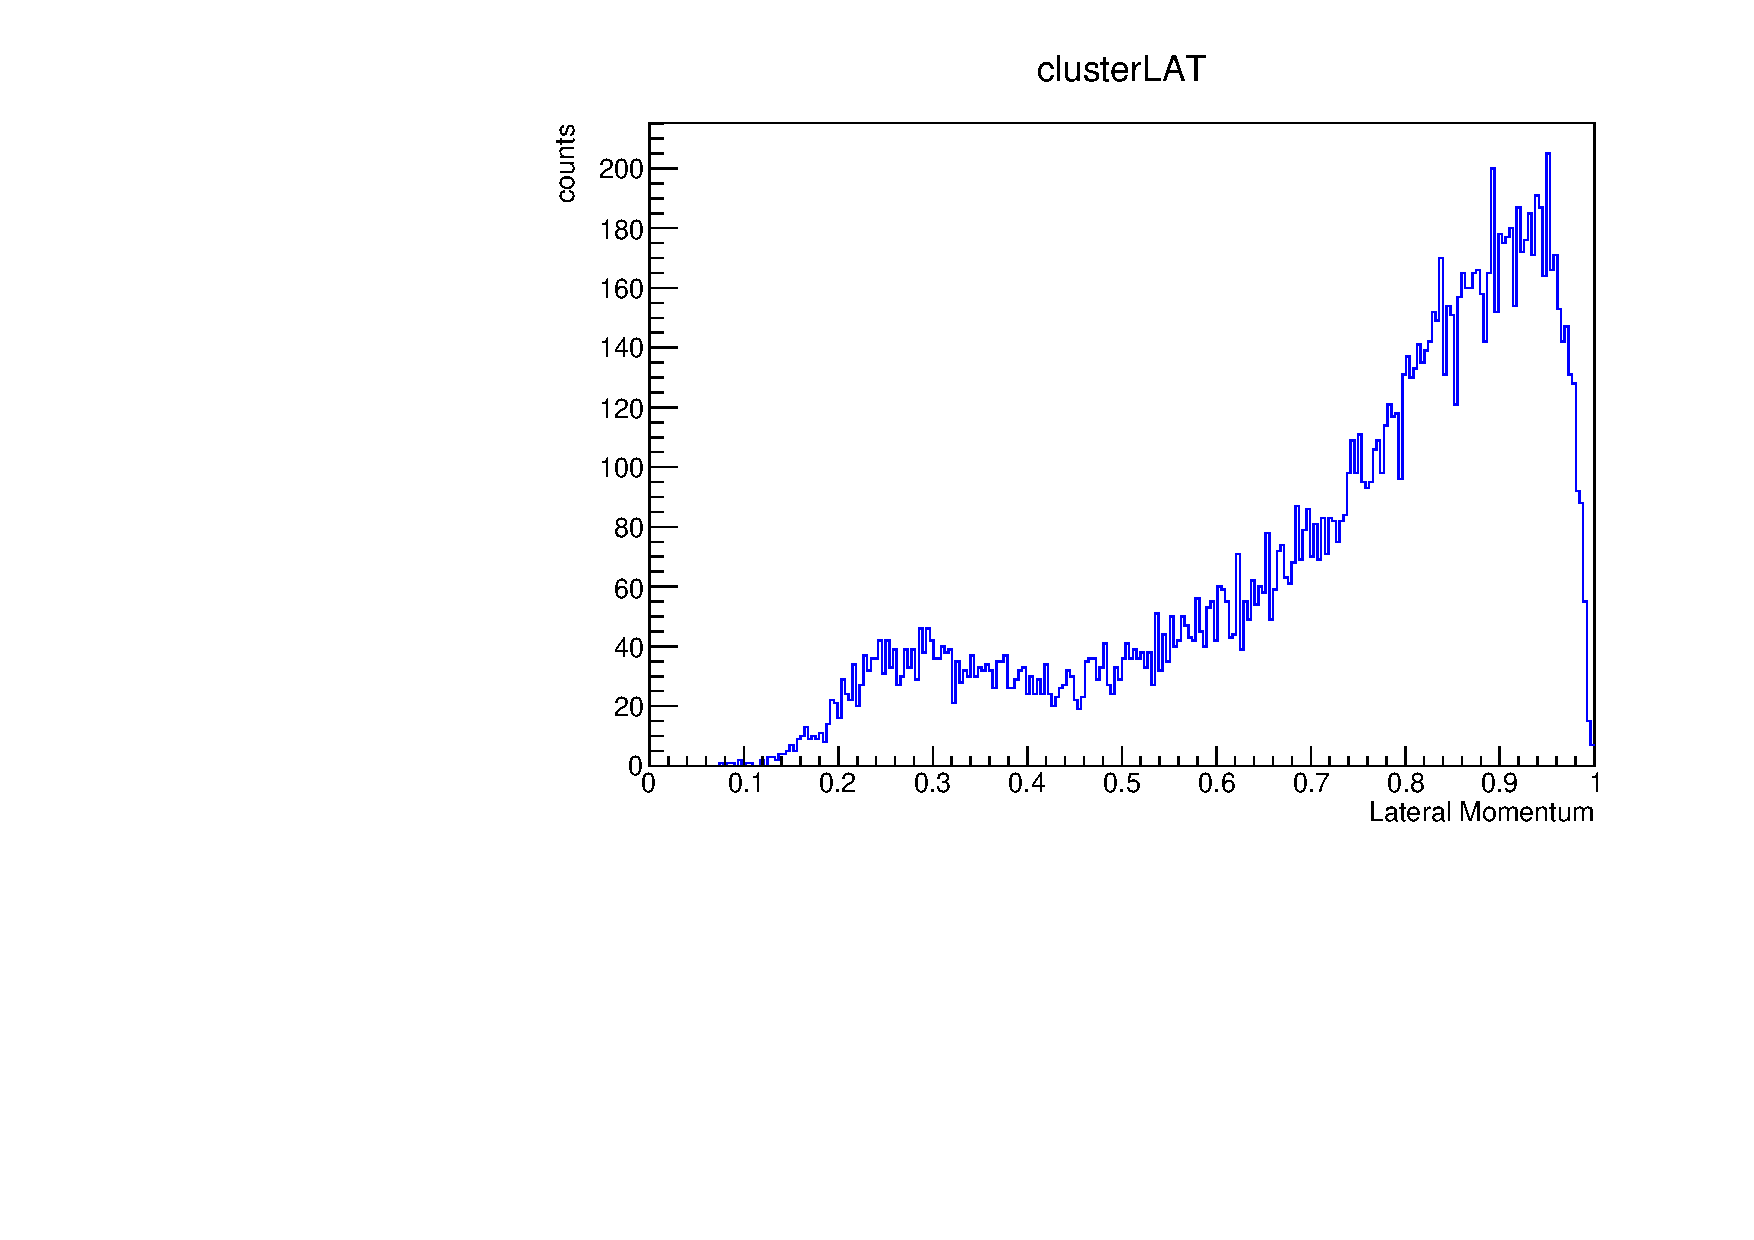
\includegraphics[width=0.49\textwidth]{nbar_cocktail/images/clusterLAT_nog_qqbar.pdf}
    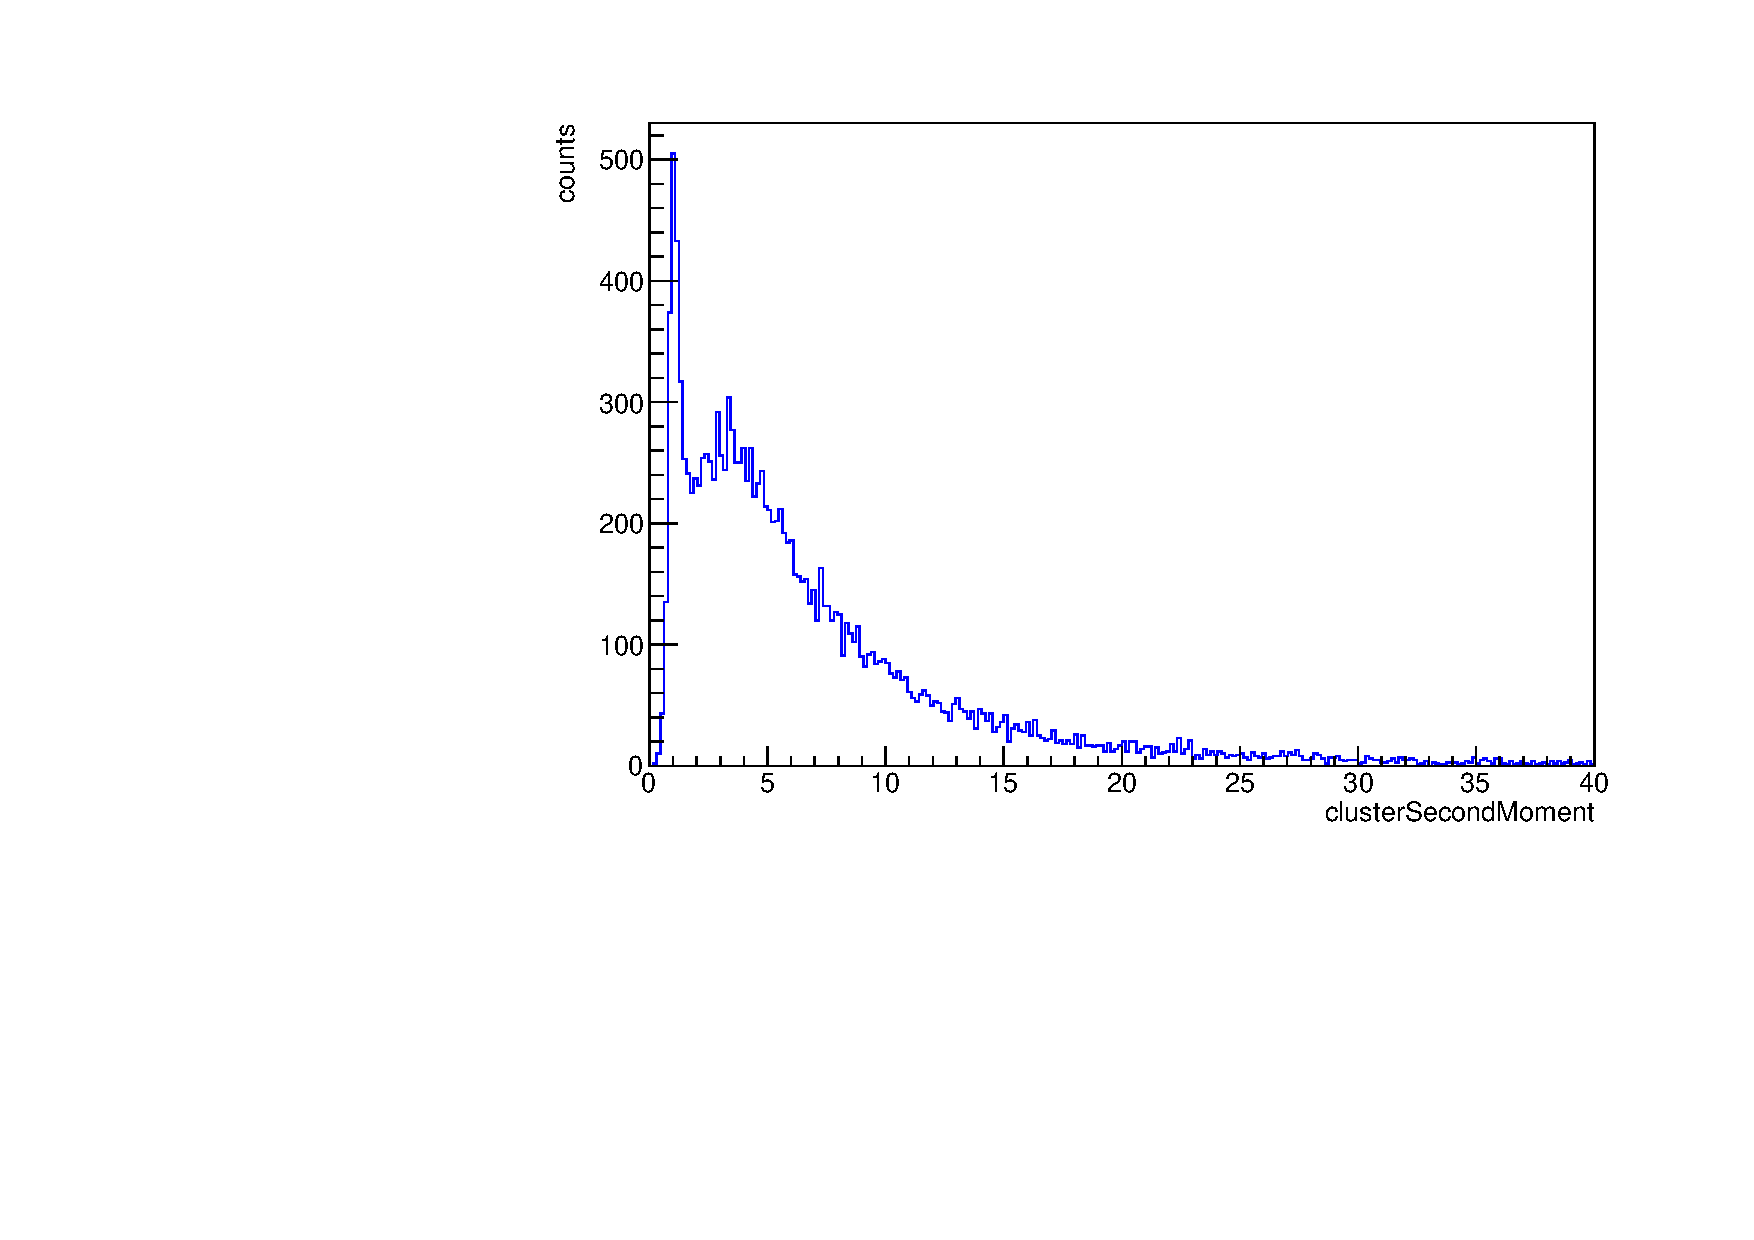
\includegraphics[width=0.49\textwidth]{nbar_cocktail/images/clusterSecondMoment_nog_qqbar.pdf}
    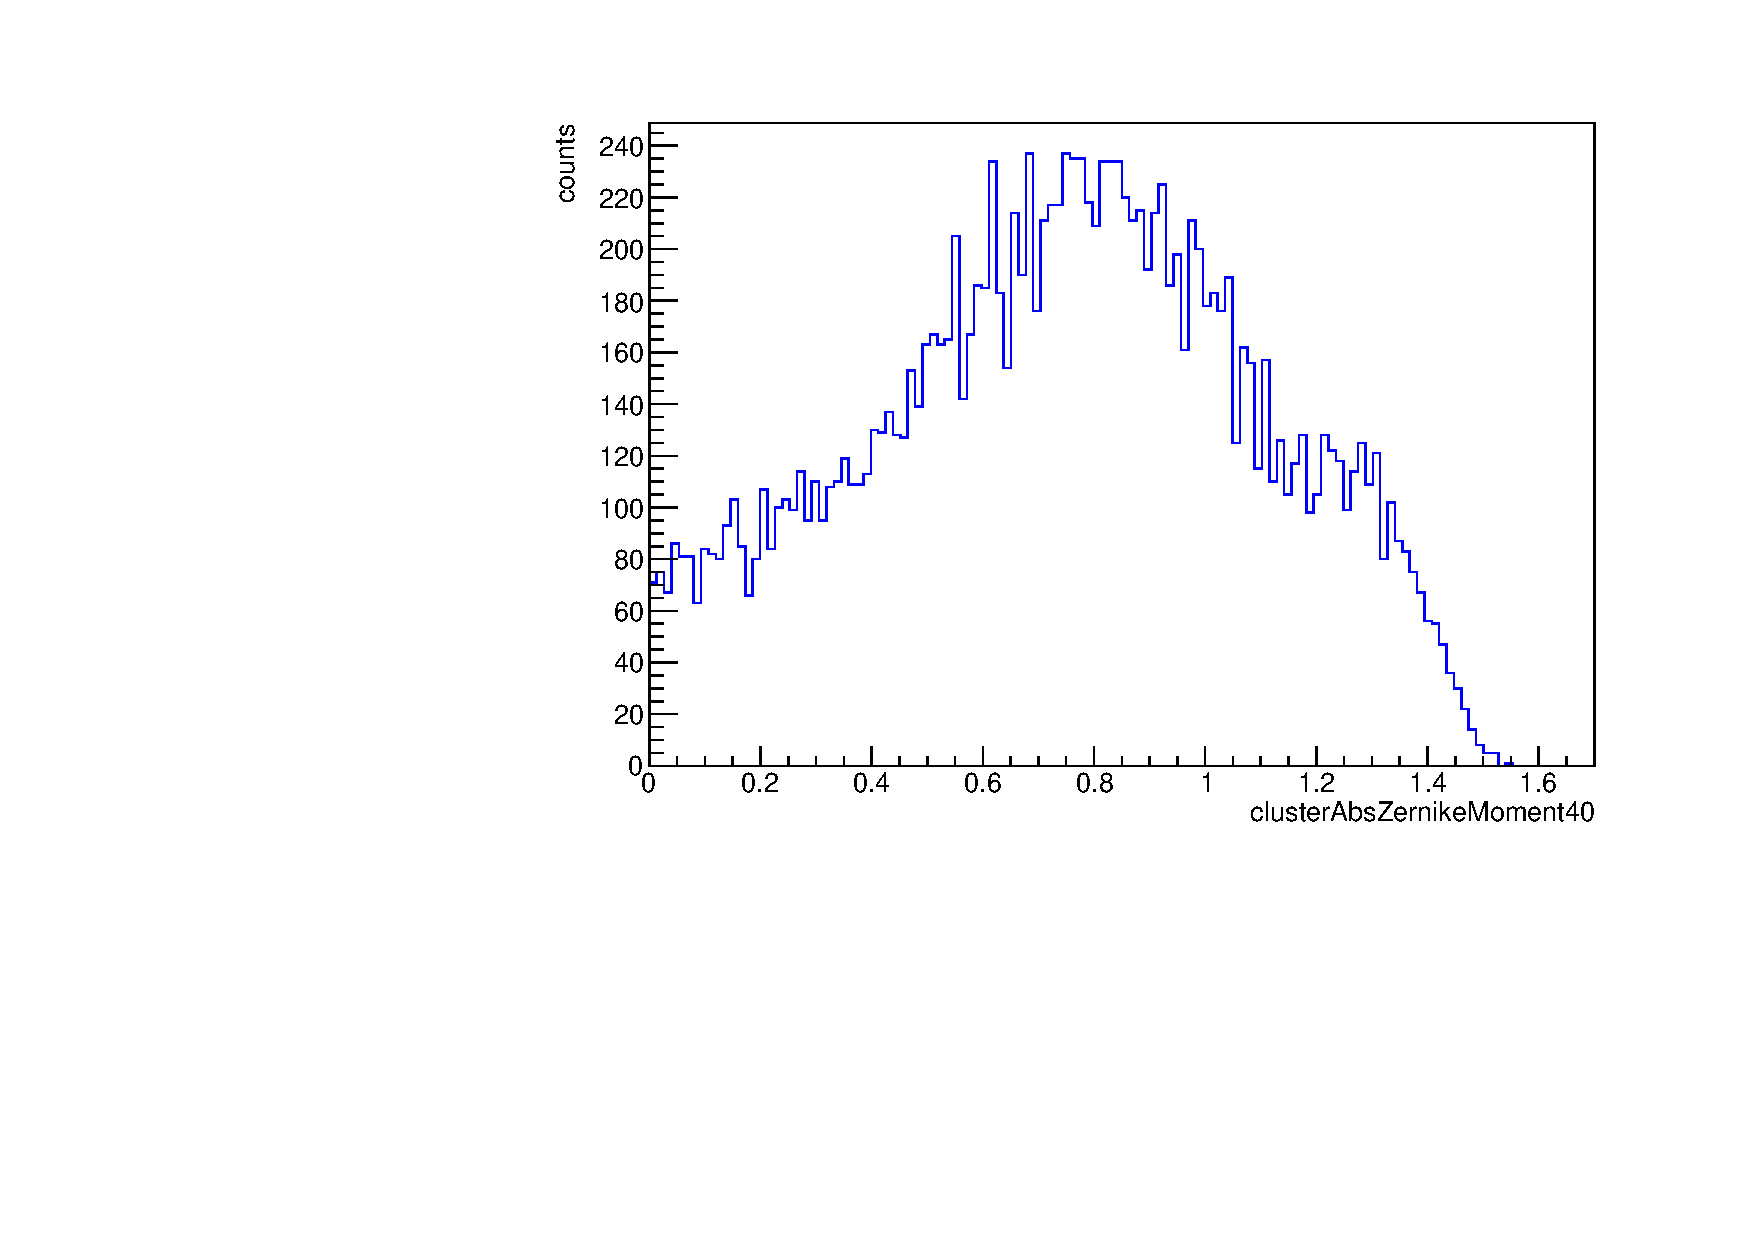
\includegraphics[width=0.49\textwidth]{nbar_cocktail/images/clusterAbsZernikeMoment40_nog_qqbar.pdf}
    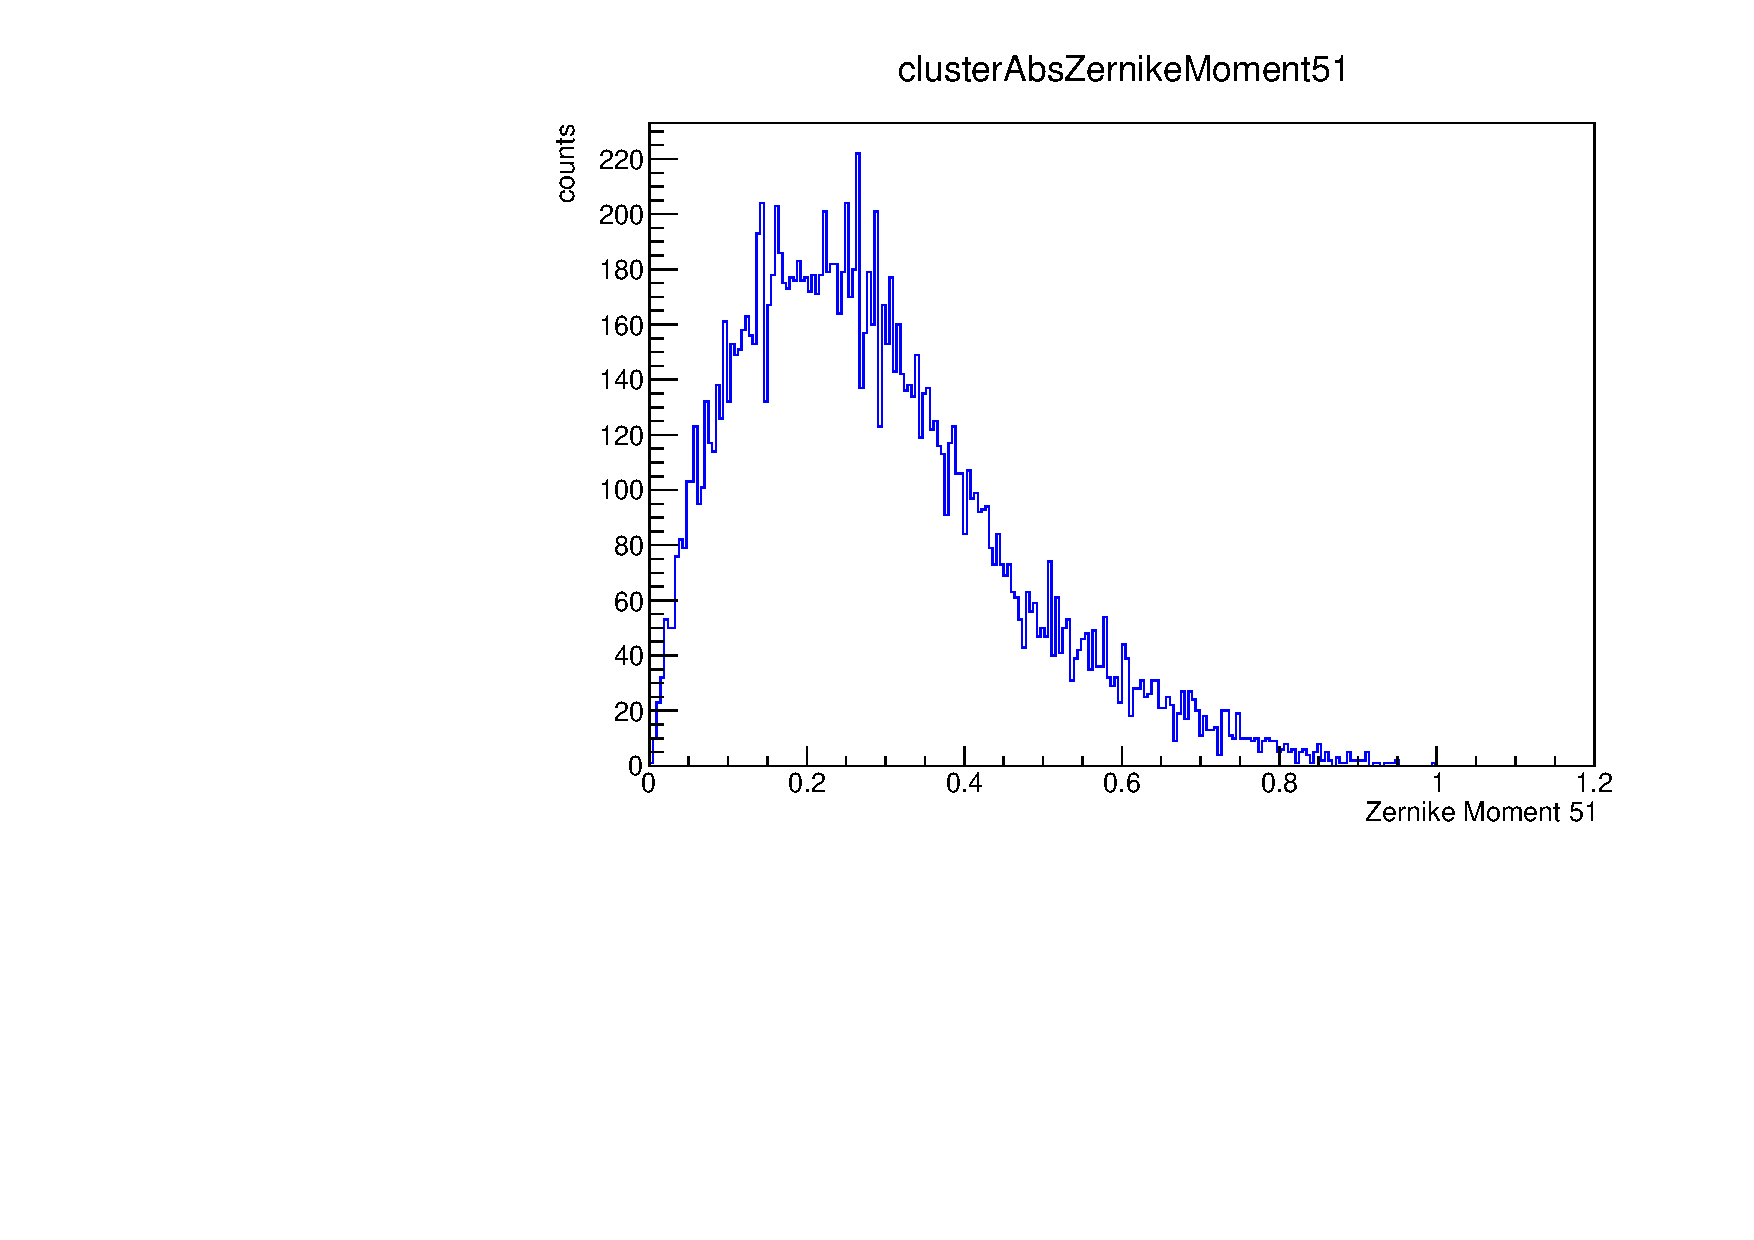
\includegraphics[width=0.49\textwidth]{nbar_cocktail/images/clusterAbsZernikeMoment51_nog_qqbar.pdf}
    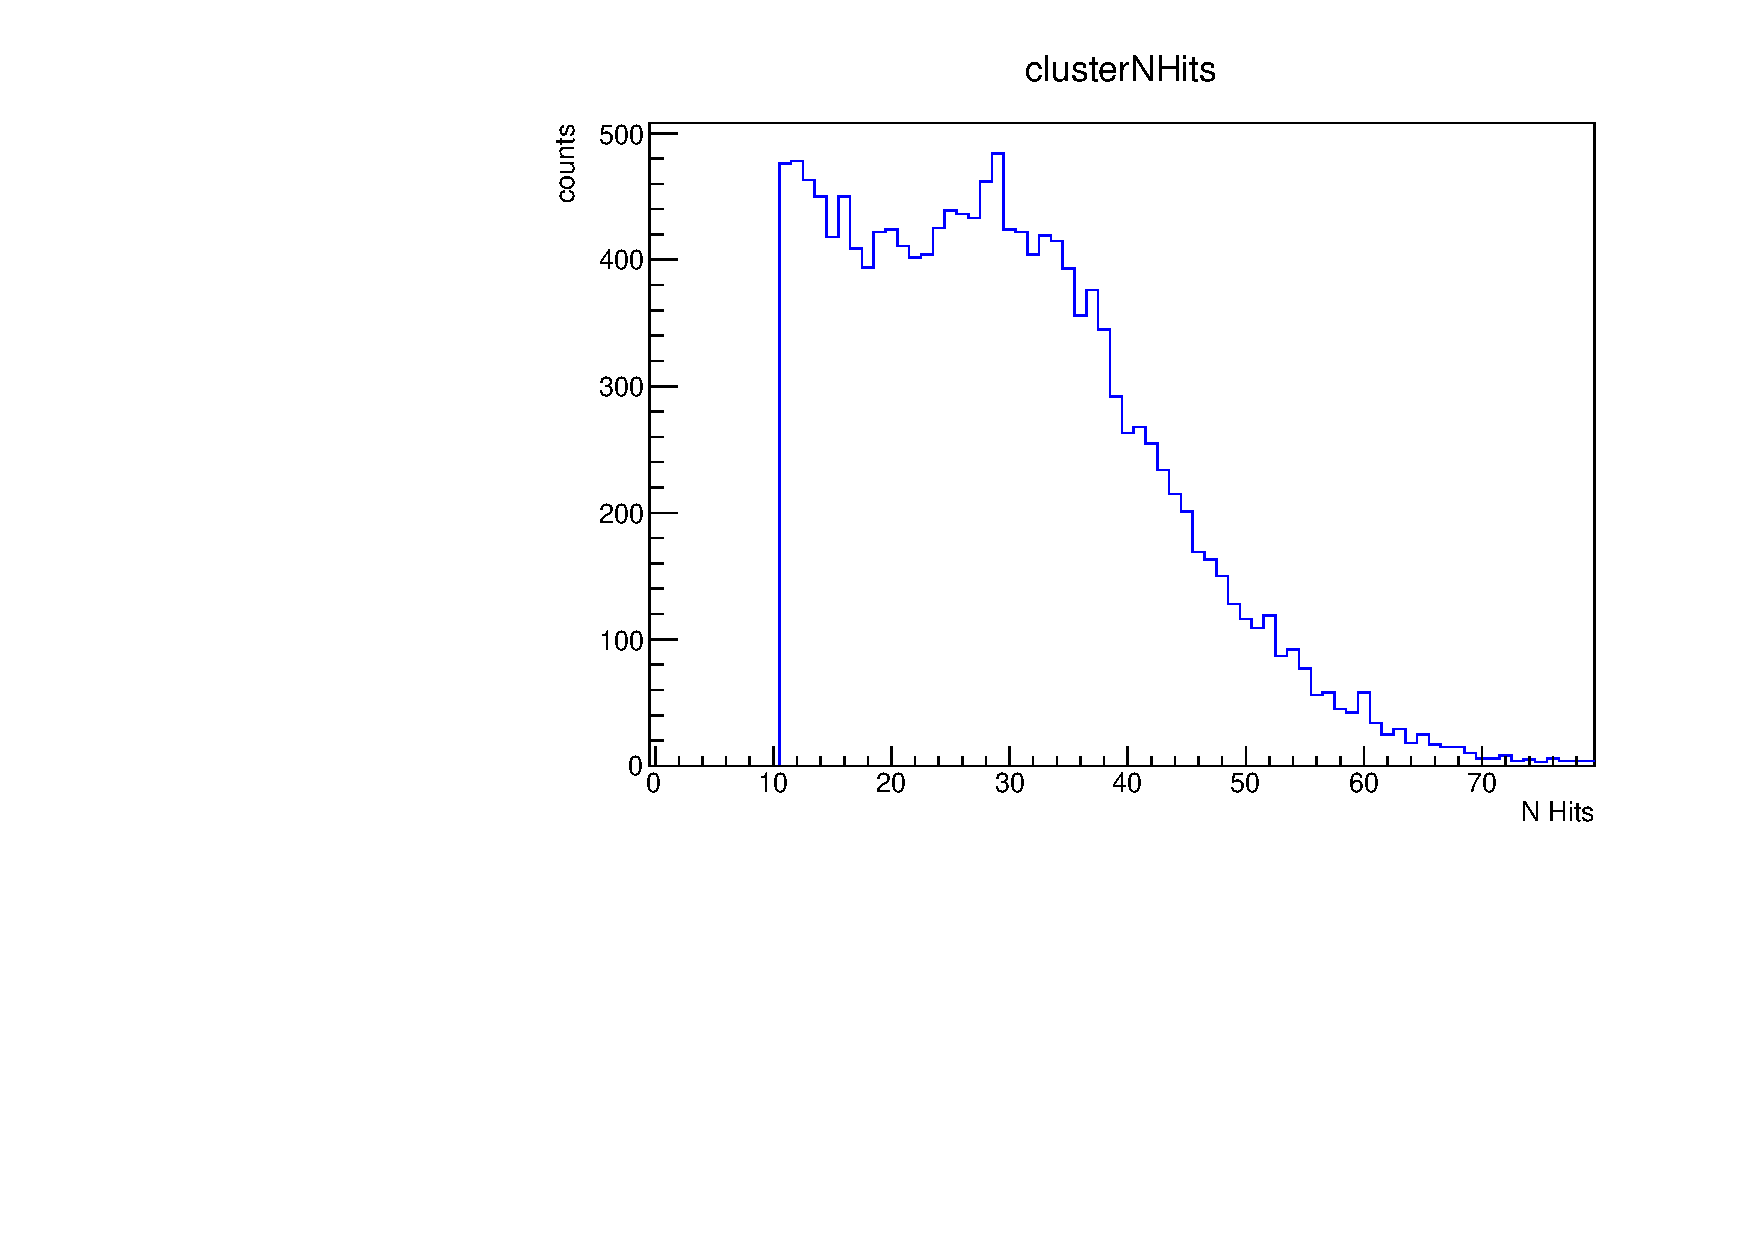
\includegraphics[width=0.49\textwidth]{nbar_cocktail/images/clusterNHits_nog_qqbar.pdf}
     \caption{Reconstructed cluster variables distribution for $\bar{n}$ candidates in the for the recoil mass region [0, 2] GeV, in NO ISR case. q$\bar{q}$ cocktail }
     \label{fig:clus_vars_nog_qqbar}
\end{figure}

\subsubsection{Sidebands technique in $q\bar{q}$ cocktail}
In order to study separately the signal and background contributions to the cluster variables, the \textbf{sidebands technique} can be adopted. 
$\\$
The sidebands technique is a data-driven method used in experimental high-energy physics to estimate and subtract the background from a region of interest. It relies on identifying a discriminating variable -often the invariant mass or the recoil mass, as this case- that separates the signal from the background. 
$\\$
The \textbf{signal region} can be defined as the region where the signal appears in the recoil mass distribution. This region contains a mixture of signal and background.
The \textbf{sidebands regions} consist of two symmetric areas (one before and one after the signal region), which may sometimes overlap, be immediately adjacent, or distant, that are assumed to contain only (or primarily) background. Therefore, in order to obtain the cluster variables distribution for the signal only, the background distribution (sidebands regions) is subtracted from the signal+background distribution (signal region) as follows:

\begin{center}
$N_{signal} = N_{\text{signal  region}} - k \cdot N_{\text{sideband region}}$,
\end{center}
where:
\begin{center}
 $k = \frac{\text{size of the signal region}}{\text{size of the sum of the sidebands regions}}$ 
 \end{center}
is a normalization factor.

$\\$
In the present case, the following region have been decided:

\begin{itemize}
\item Signal region: [0.8, 1.2] GeV;
\item Sidebands regions: [0.3, 0.7] U [1.3, 1.7]  GeV;
\item $k = \frac{1.2 - 0.8}{(0.7 - 0.3) + (1.7 - 1.3)} = \frac{1}{2}$.
\end{itemize}

The signal region and sidebands region, in the recoil mass distribution observed in Fig.~\ref{fig:mRecComps_nog_010_qqbar}, are shown in Fig.\ref{fig:recMass_sidebands}.
\begin{figure}[H]
    \centering
    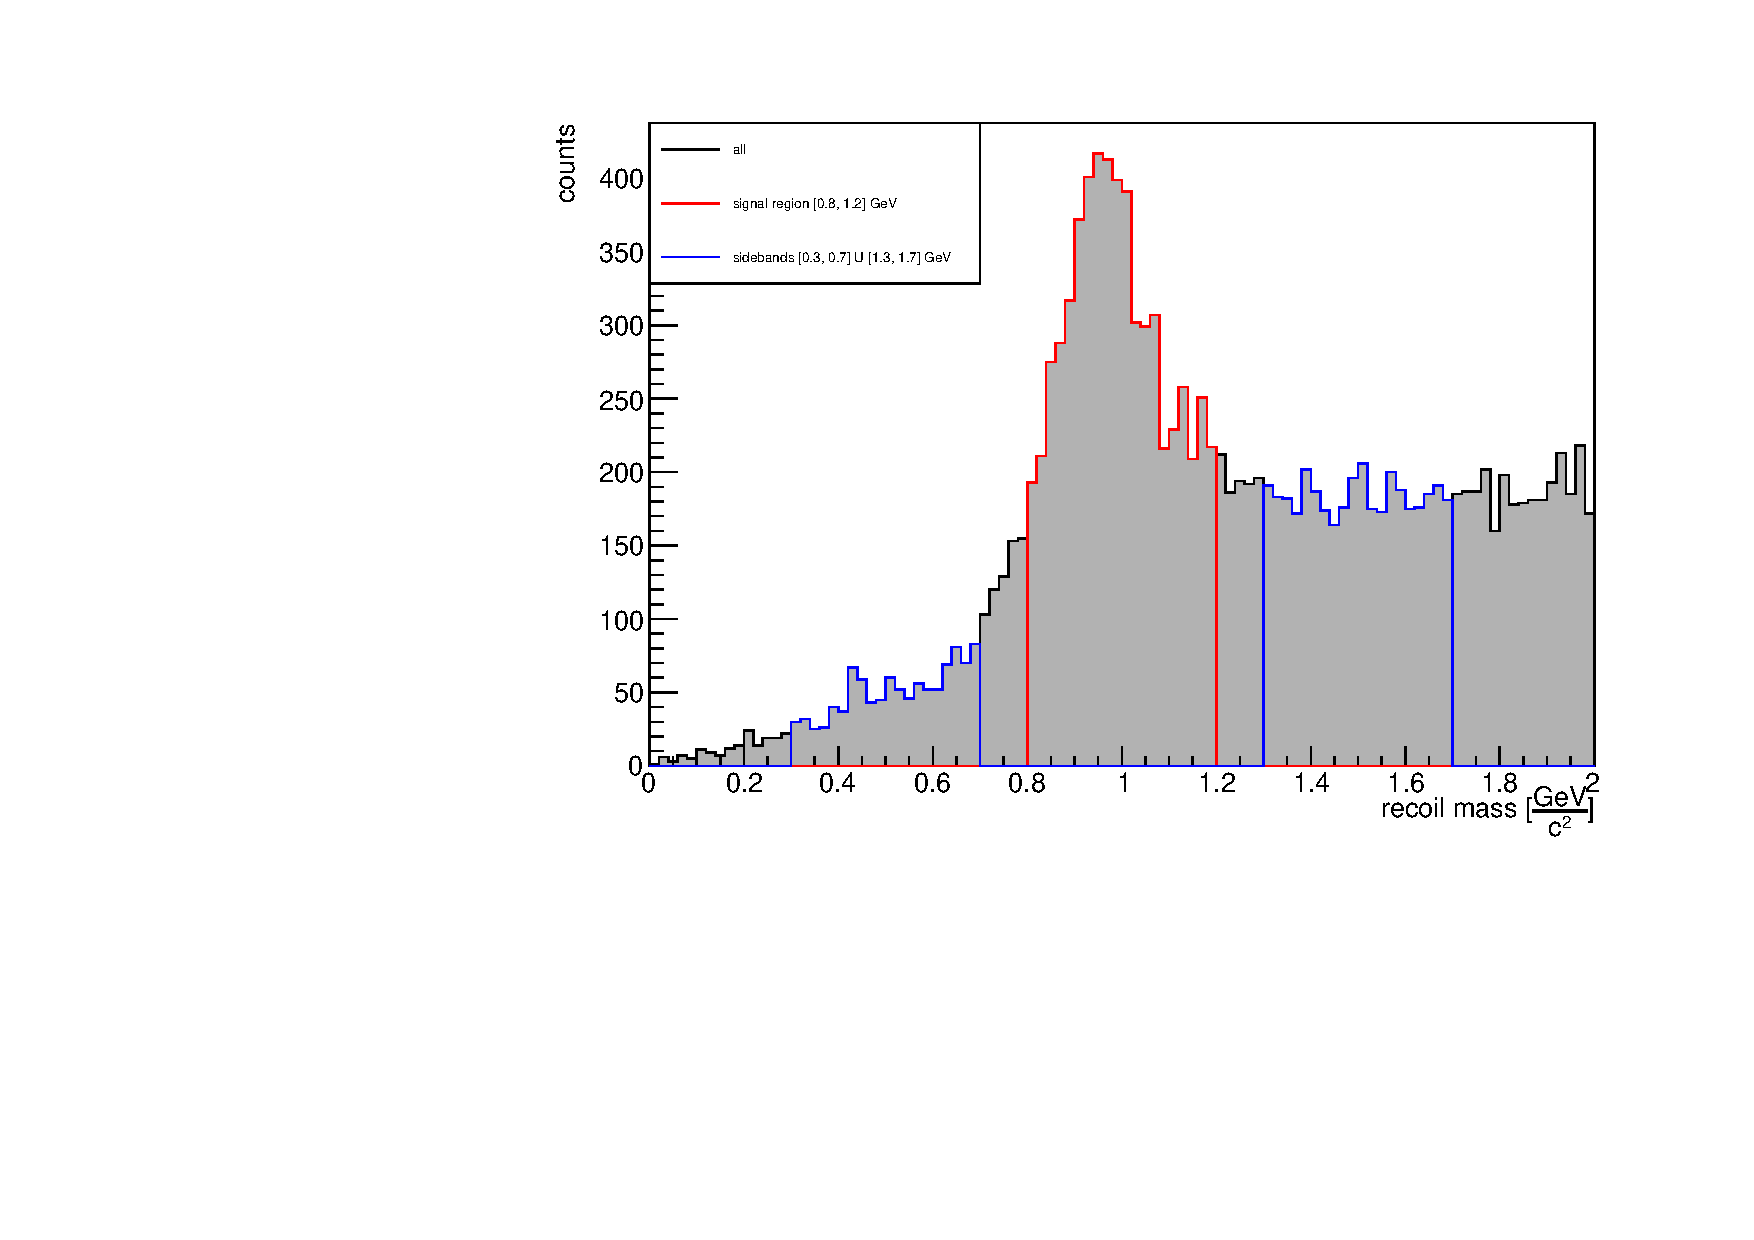
\includegraphics[width=0.6\textwidth]{nbar_cocktail/images/recoil_mass_sidebands_nog}
    \caption{Recoil mass distribution (black), with the signal region (red) and the sidebands regions (blue), in the $q\bar{q}$ Monte Carlo cocktail. NO ISR case.}
    \label{fig:recMass_sidebands}
\end{figure}
$\\$
The single contributions from the signal region and the two sidebands regions to the cluster variable can be compared. Since the two sidebands regions combined are two times larger than the signal region, a scaling factor of $k = 0.5$ has been applied to the cluster variables obtained from the sidebands regions. The obtained cluster variables contribution is shown in Fig.\ref{fig:clus_vars_sidebands_pre}.
 \begin{figure}[h]
    \centering
    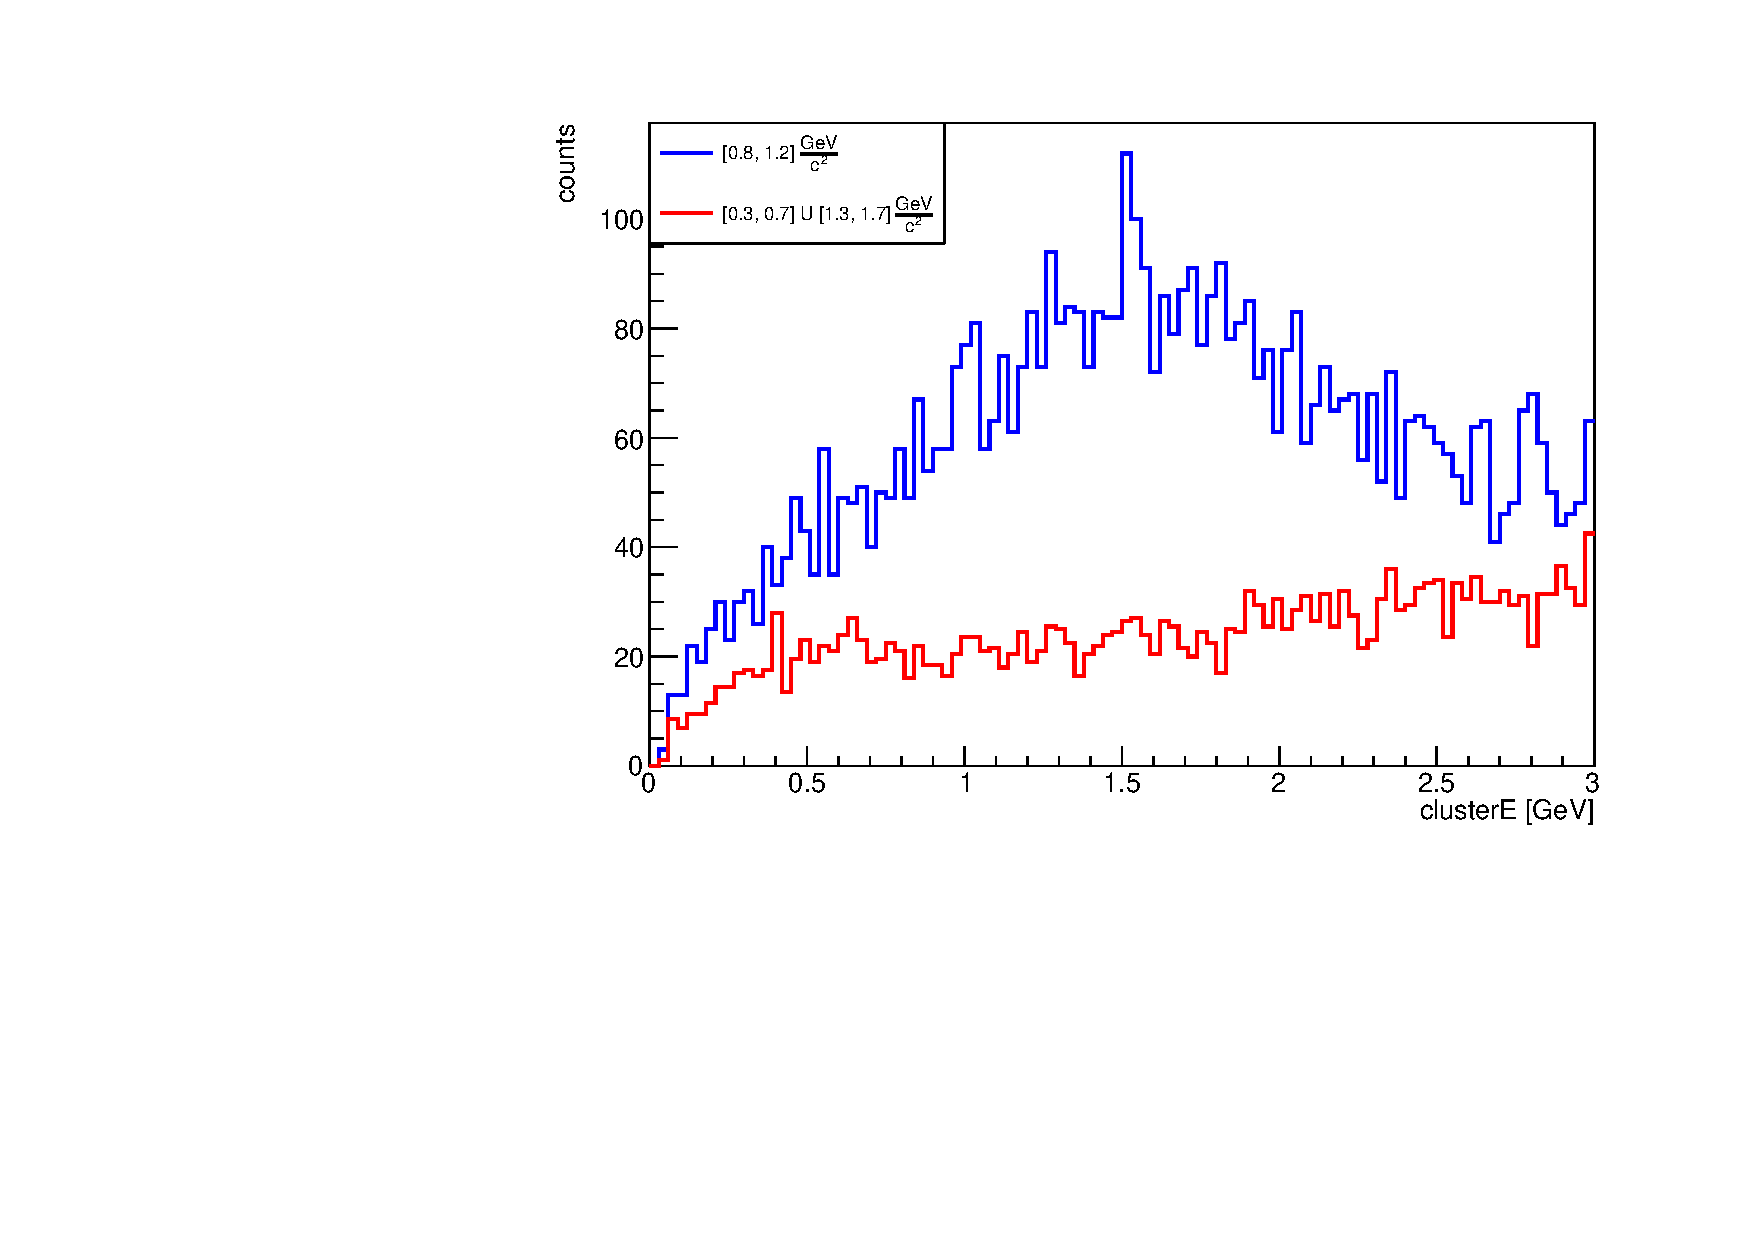
\includegraphics[width=0.49\textwidth]{nbar_cocktail/images/sidebands_clusterE_nog.pdf}
    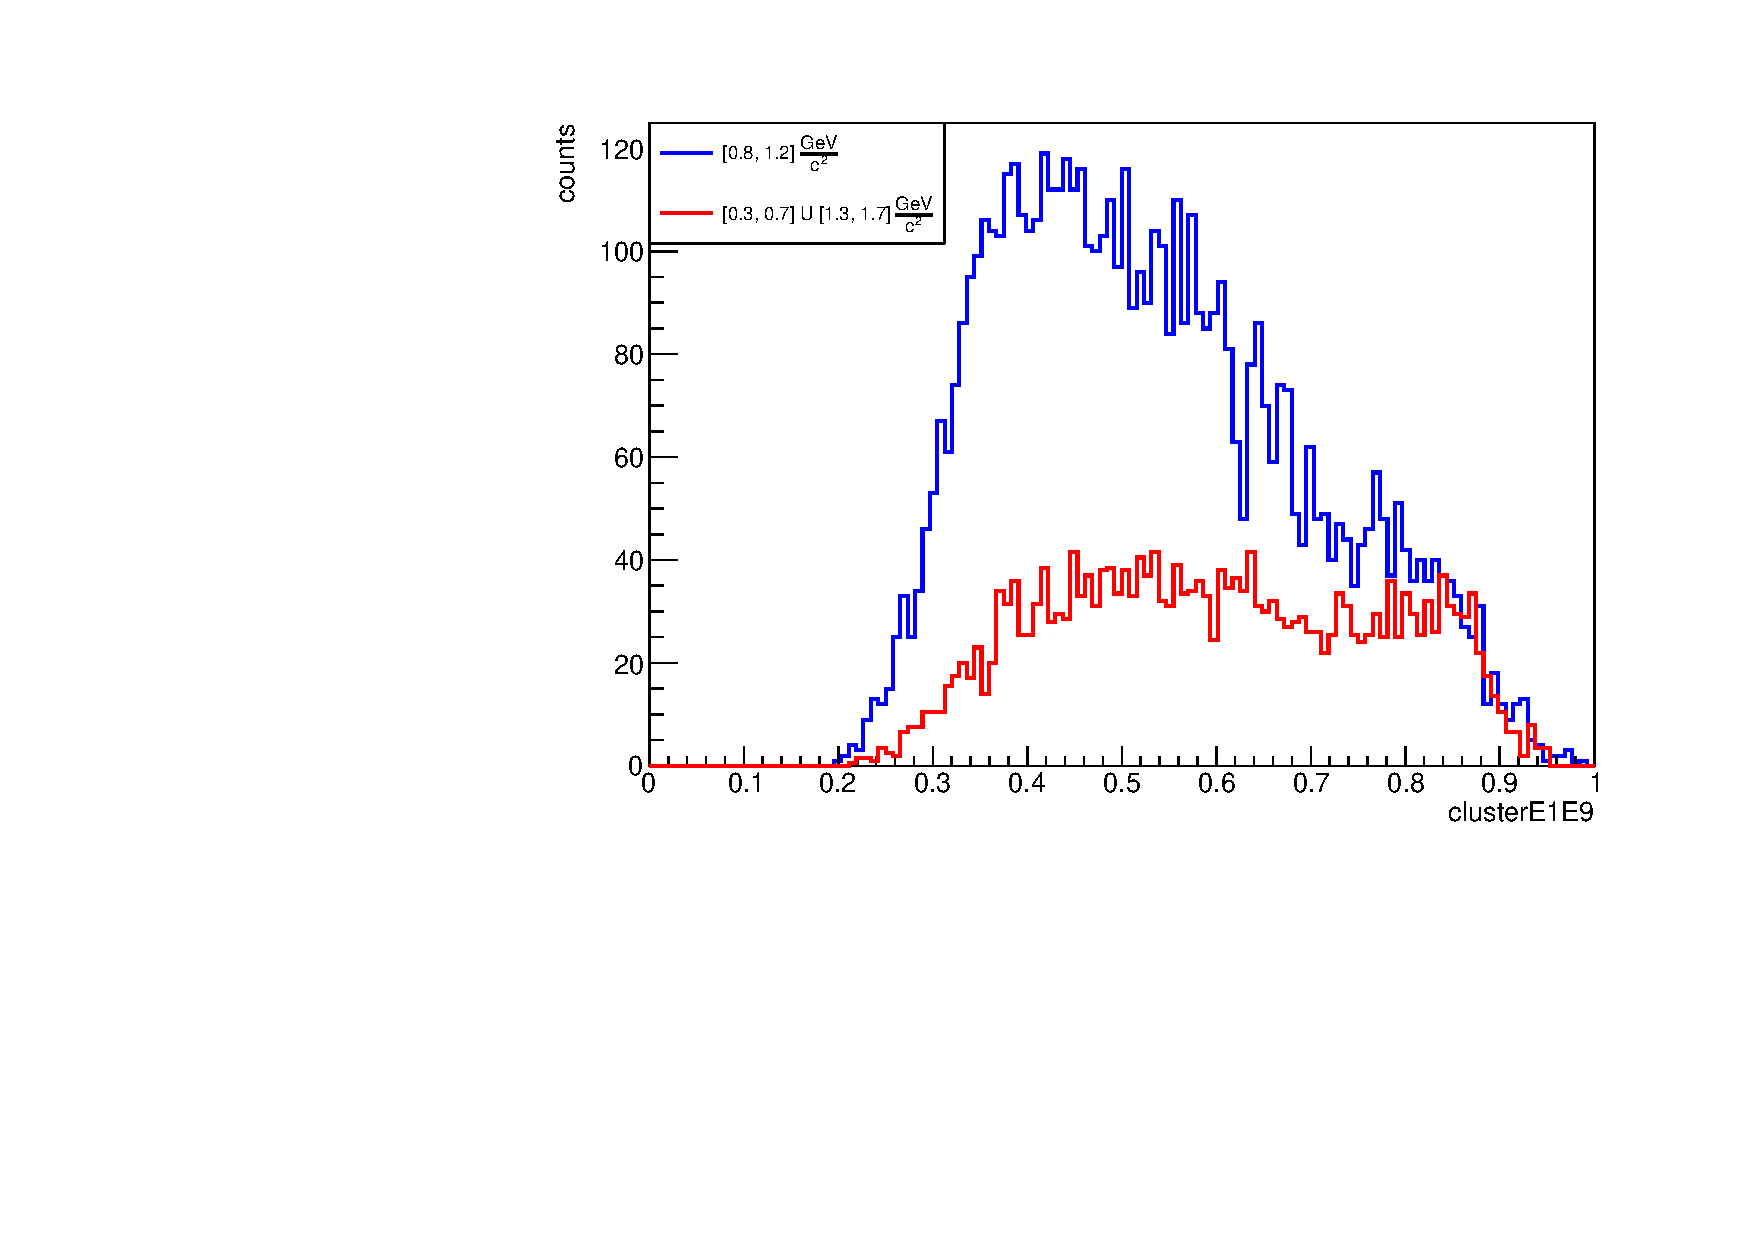
\includegraphics[width=0.49\textwidth]{nbar_cocktail/images/sidebands_clusterE1E9_nog.pdf}
    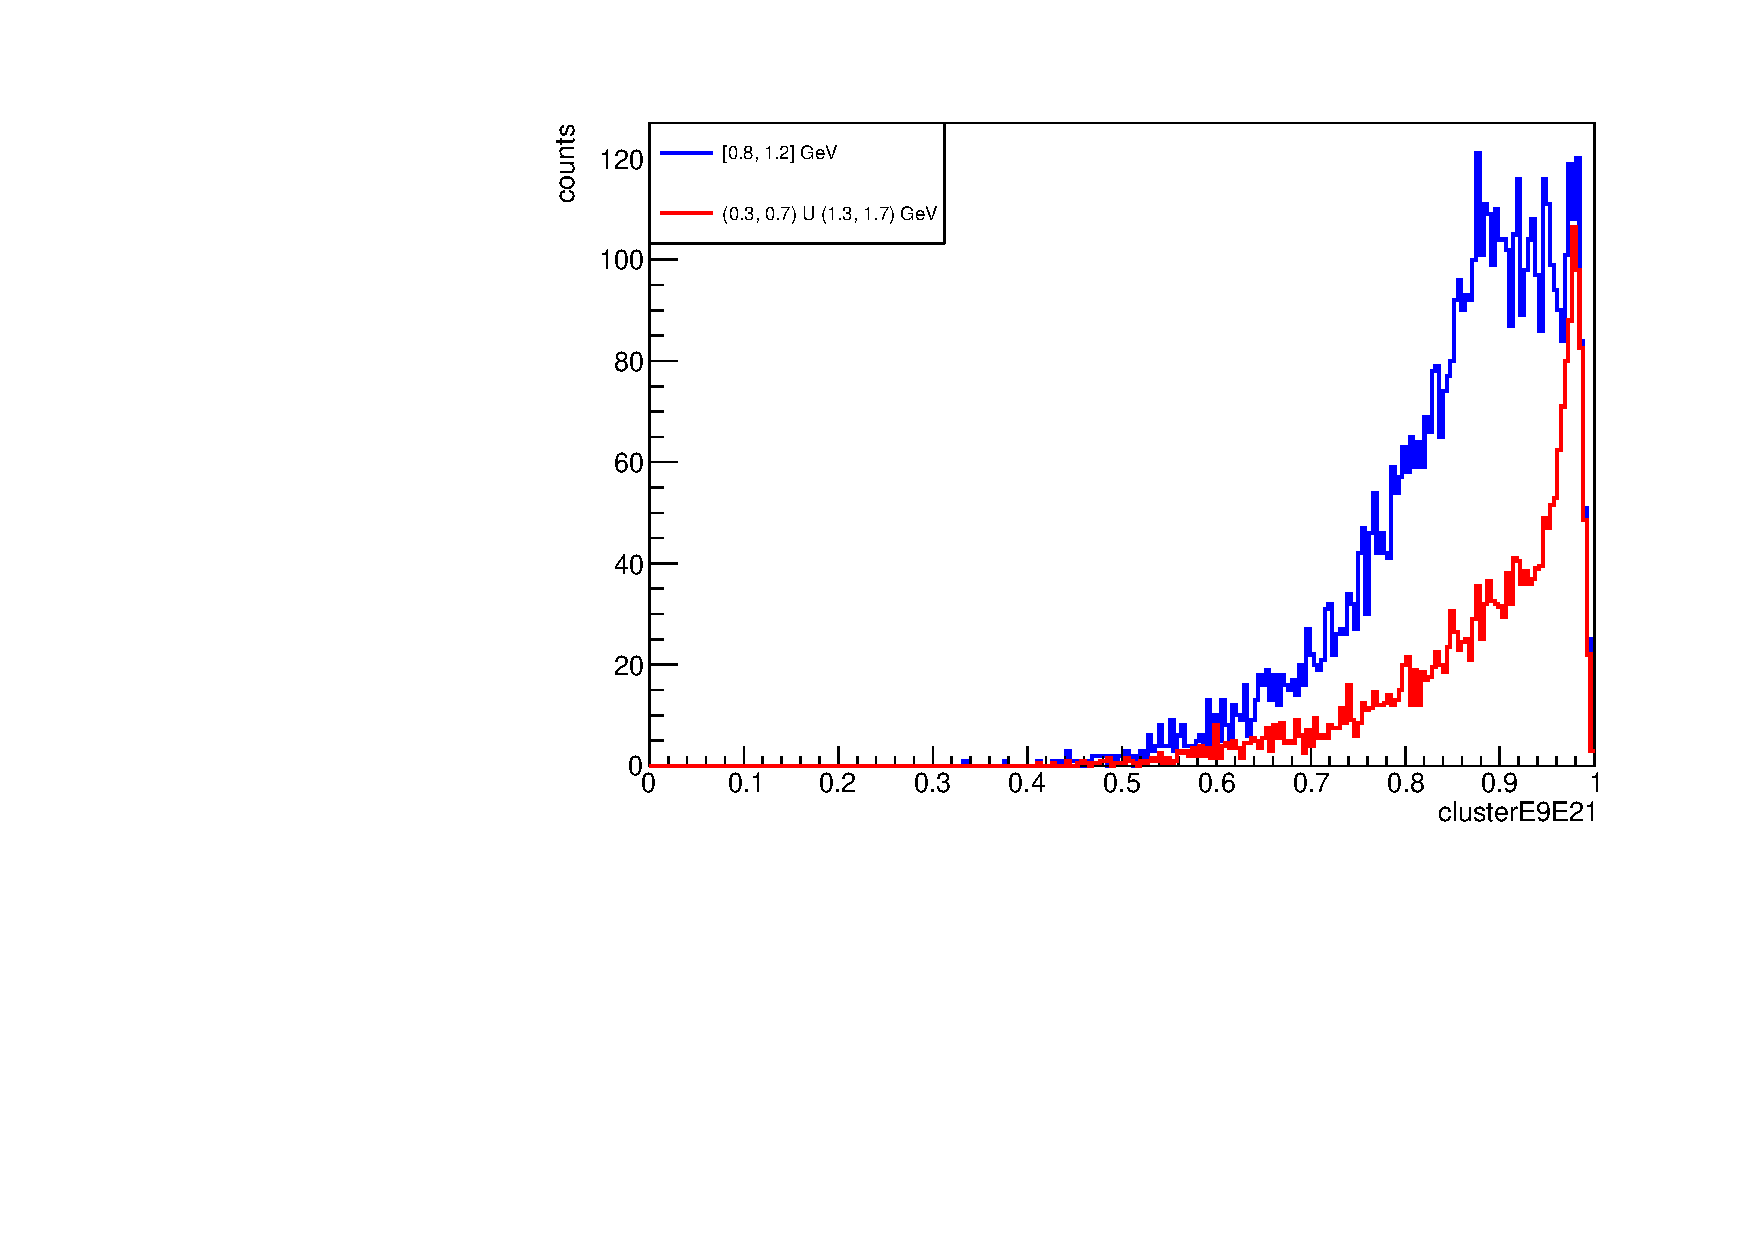
\includegraphics[width=0.49\textwidth]{nbar_cocktail/images/sidebands_clusterE9E21_nog.pdf}
    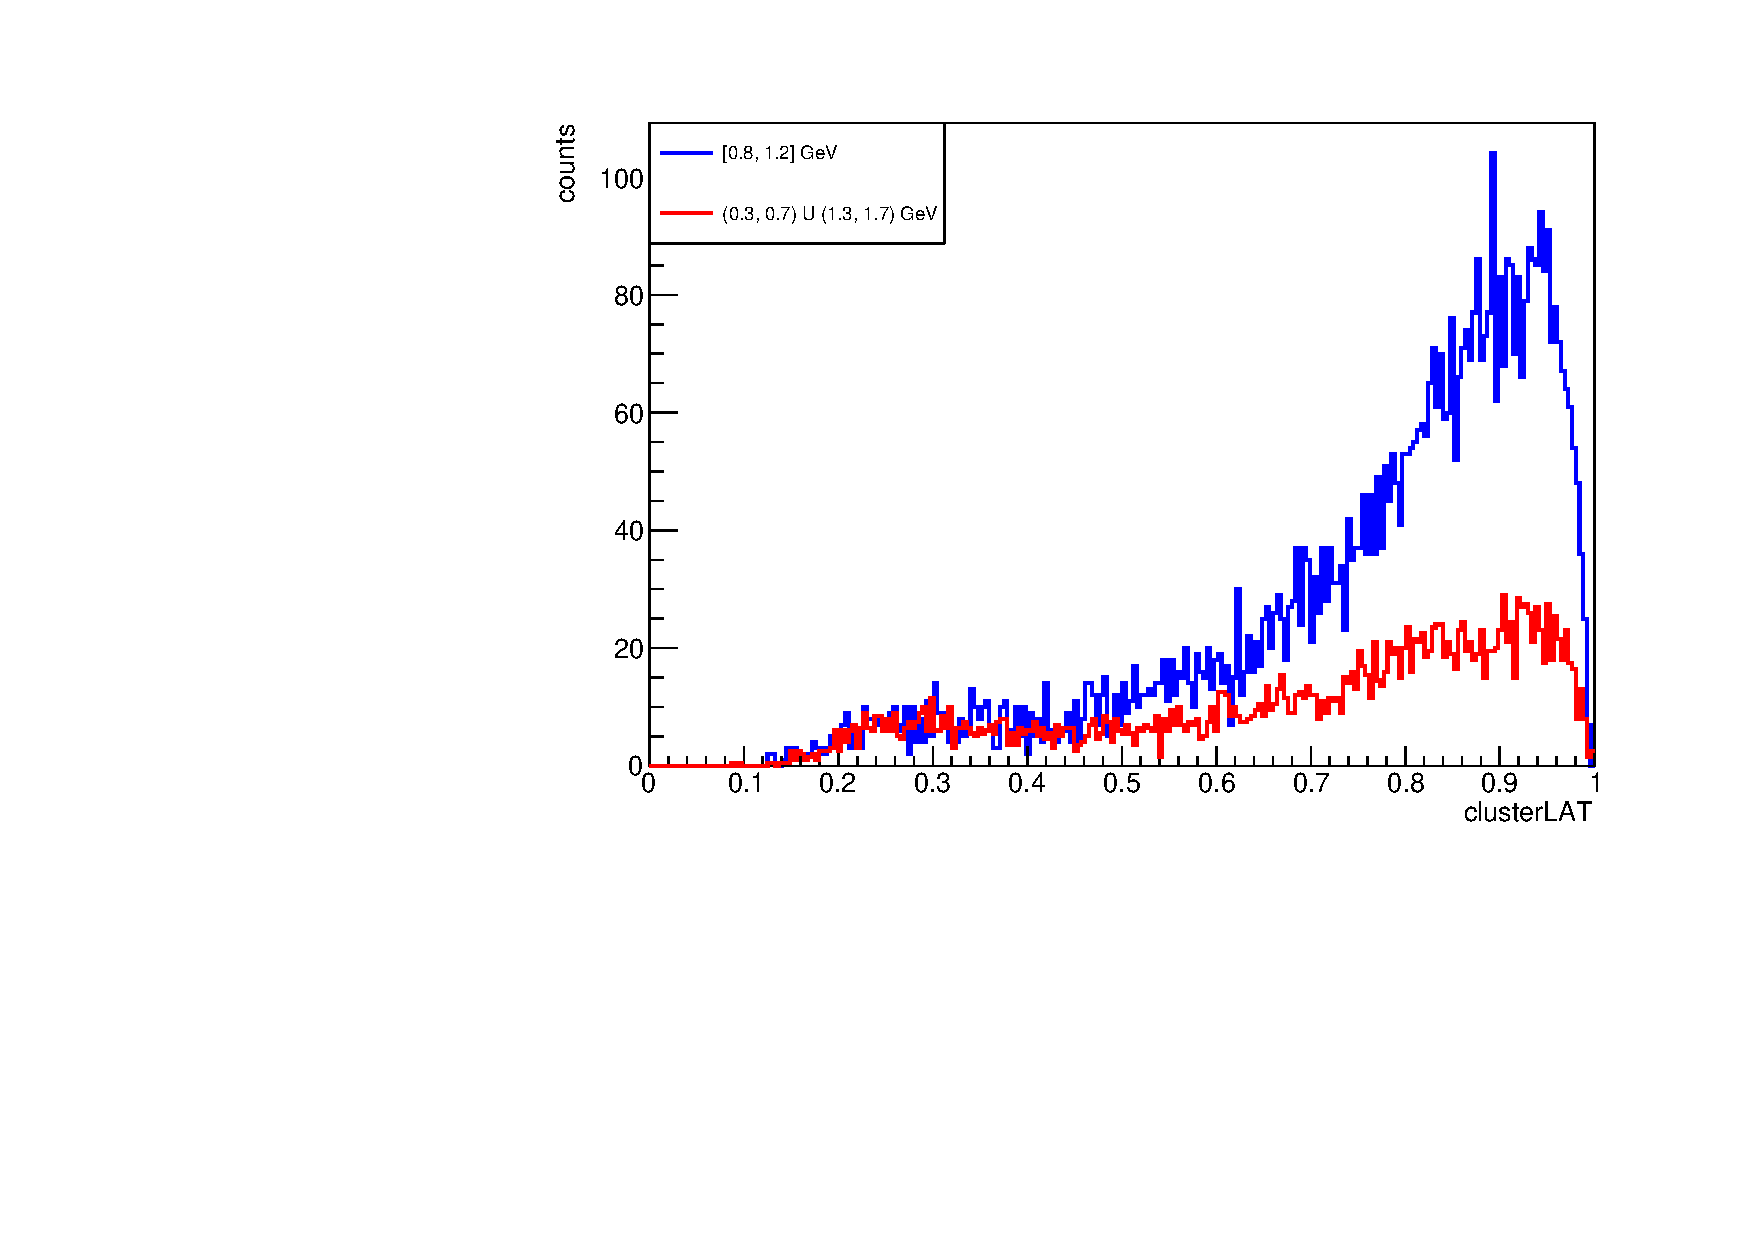
\includegraphics[width=0.49\textwidth]{nbar_cocktail/images/sidebands_clusterLAT_nog.pdf}
    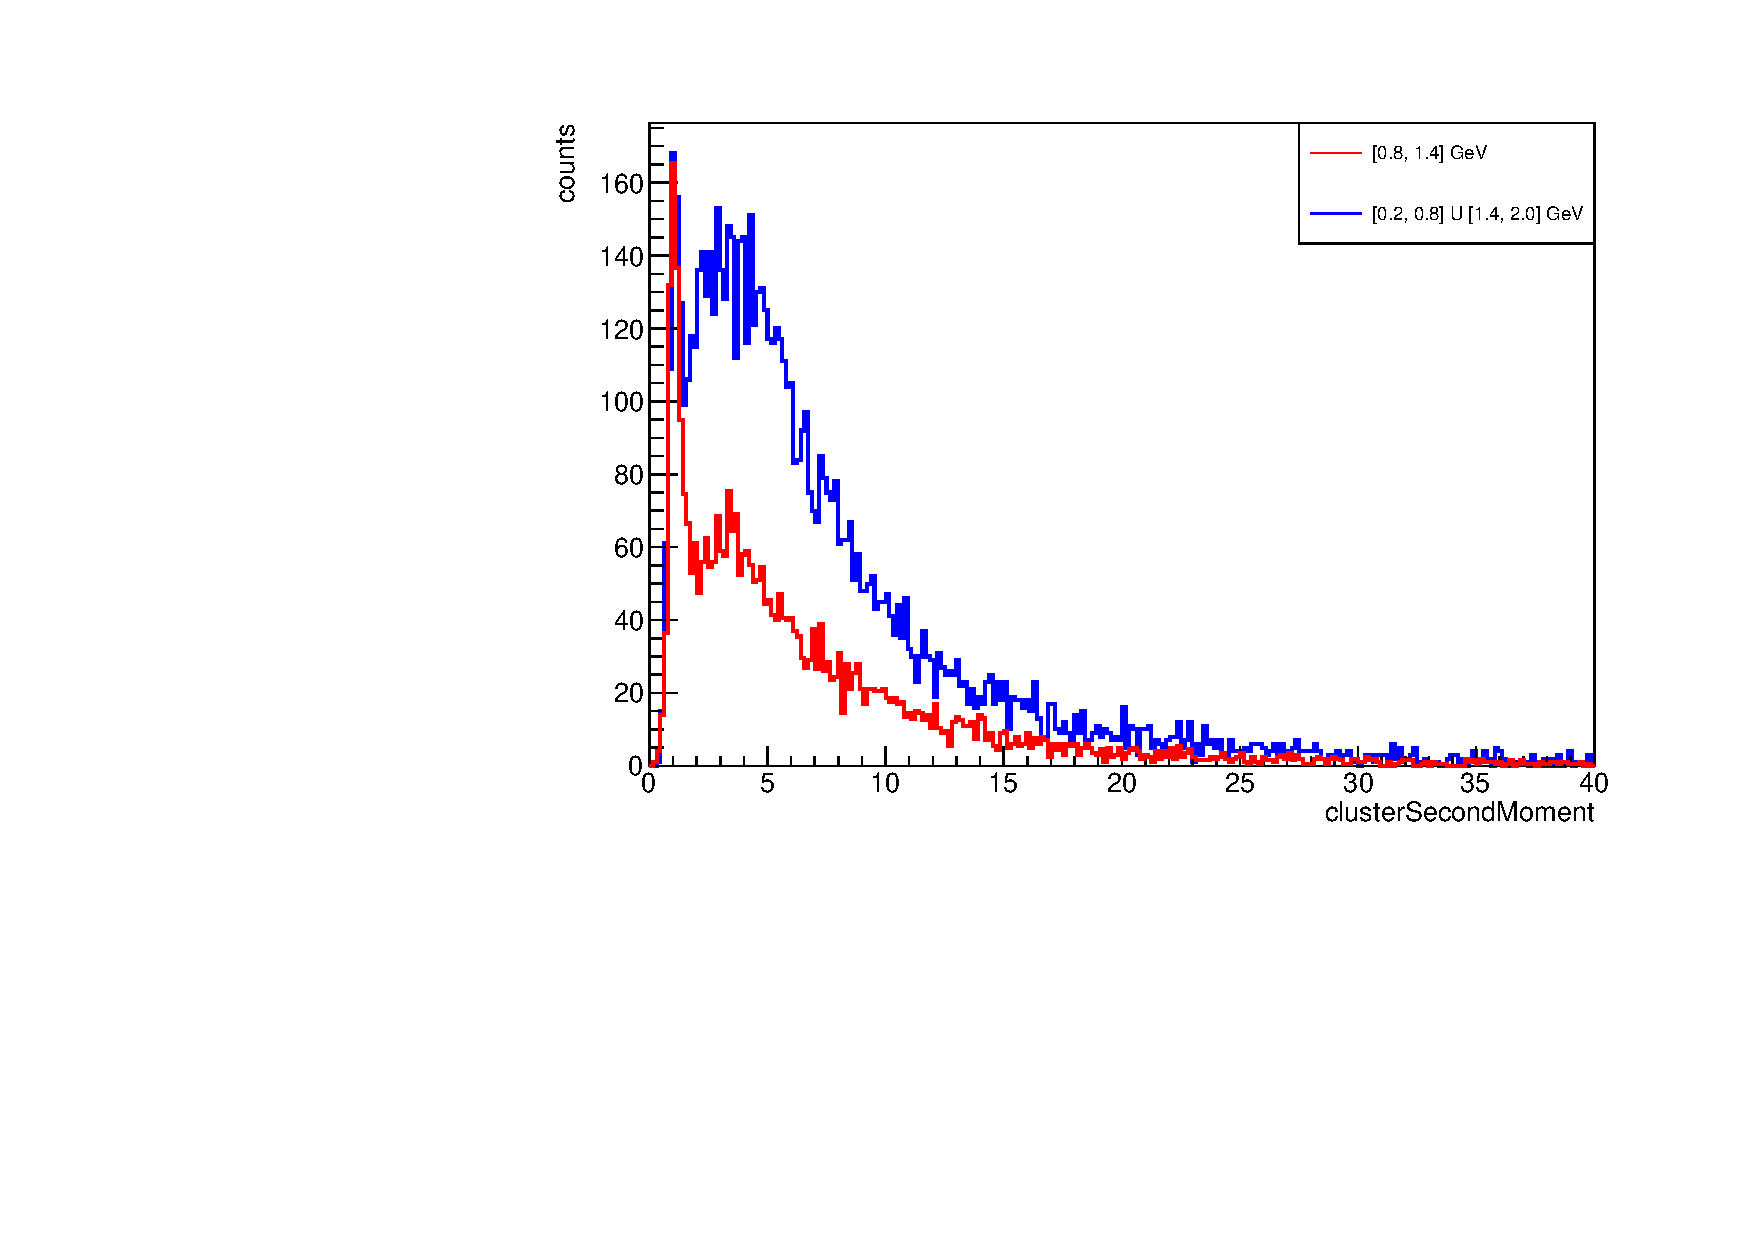
\includegraphics[width=0.49\textwidth]{nbar_cocktail/images/sidebands_clusterSecondMoment_nog.pdf}
    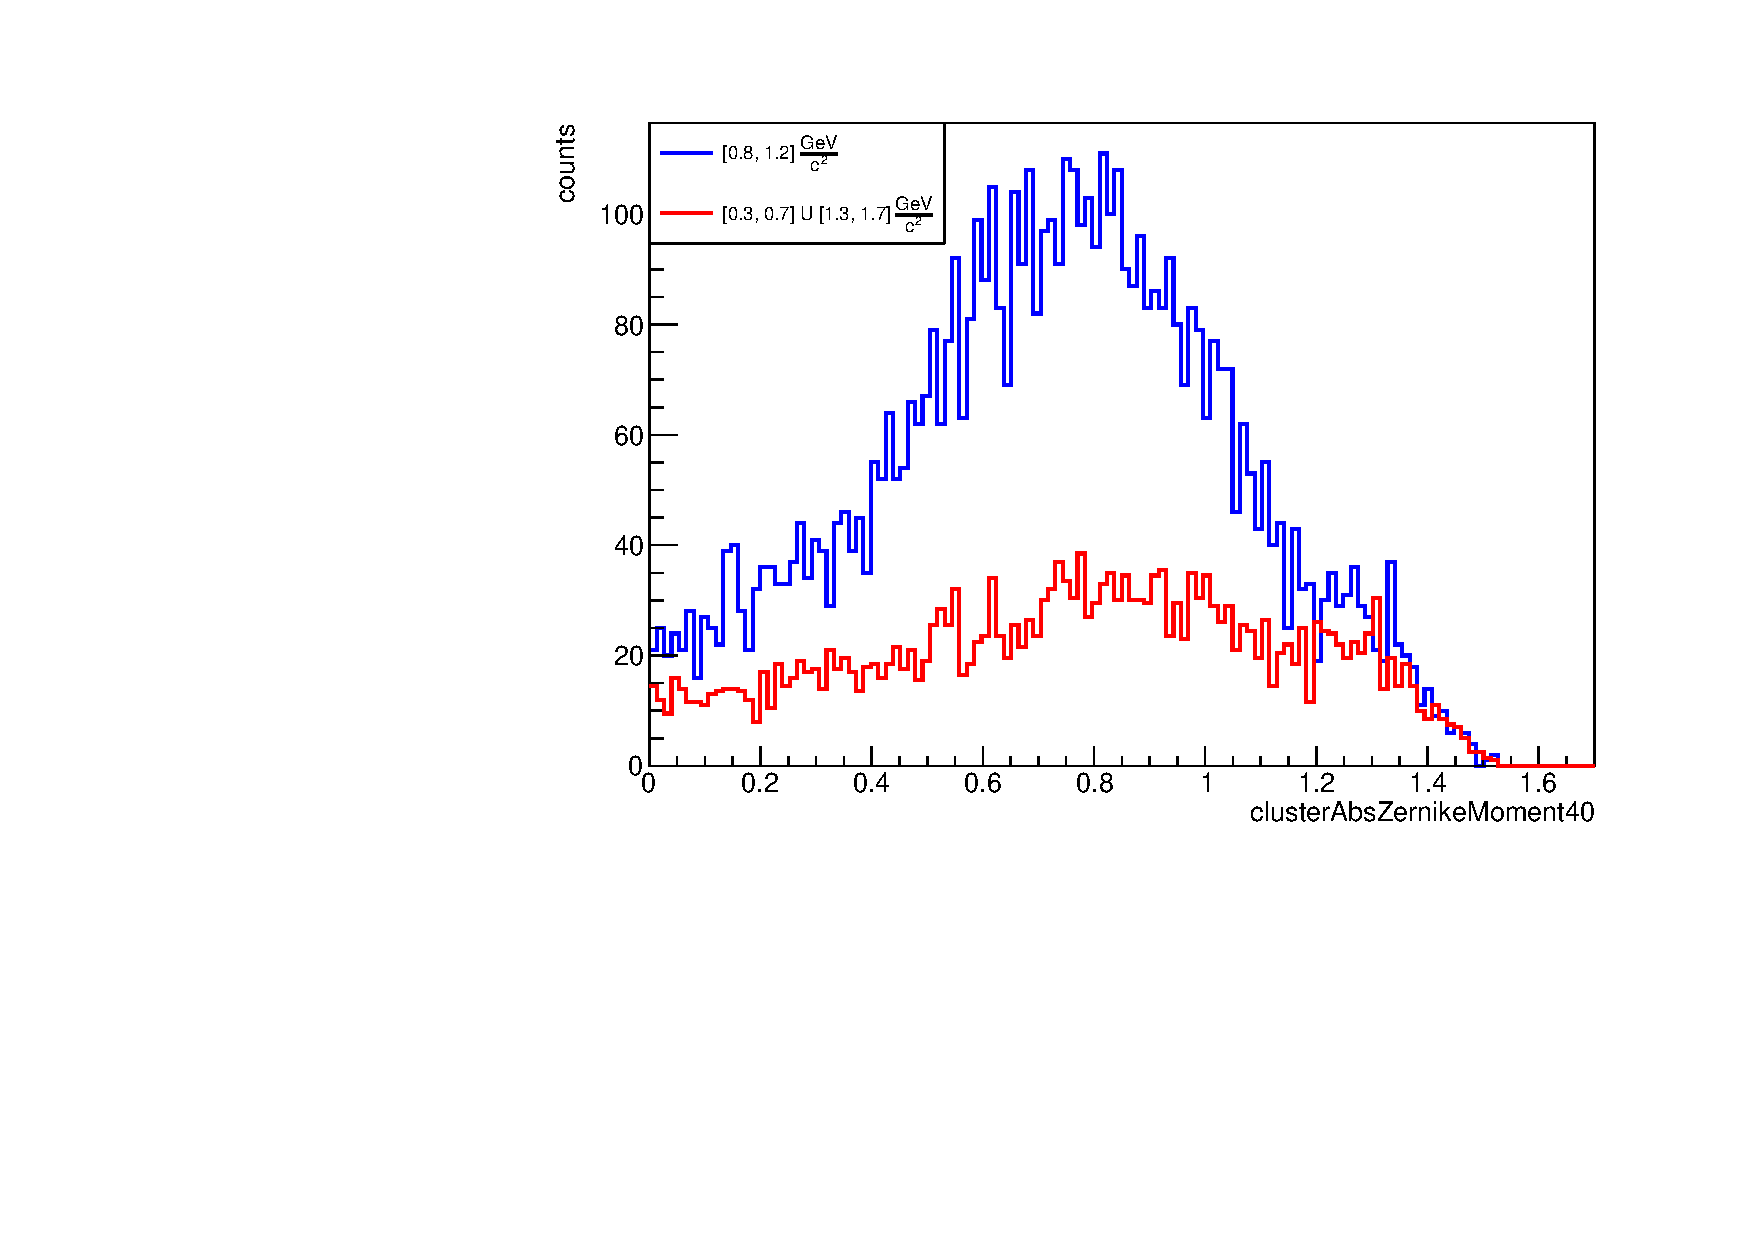
\includegraphics[width=0.49\textwidth]{nbar_cocktail/images/sidebands_clusterAbsZernikeMoment40_nog.pdf}
    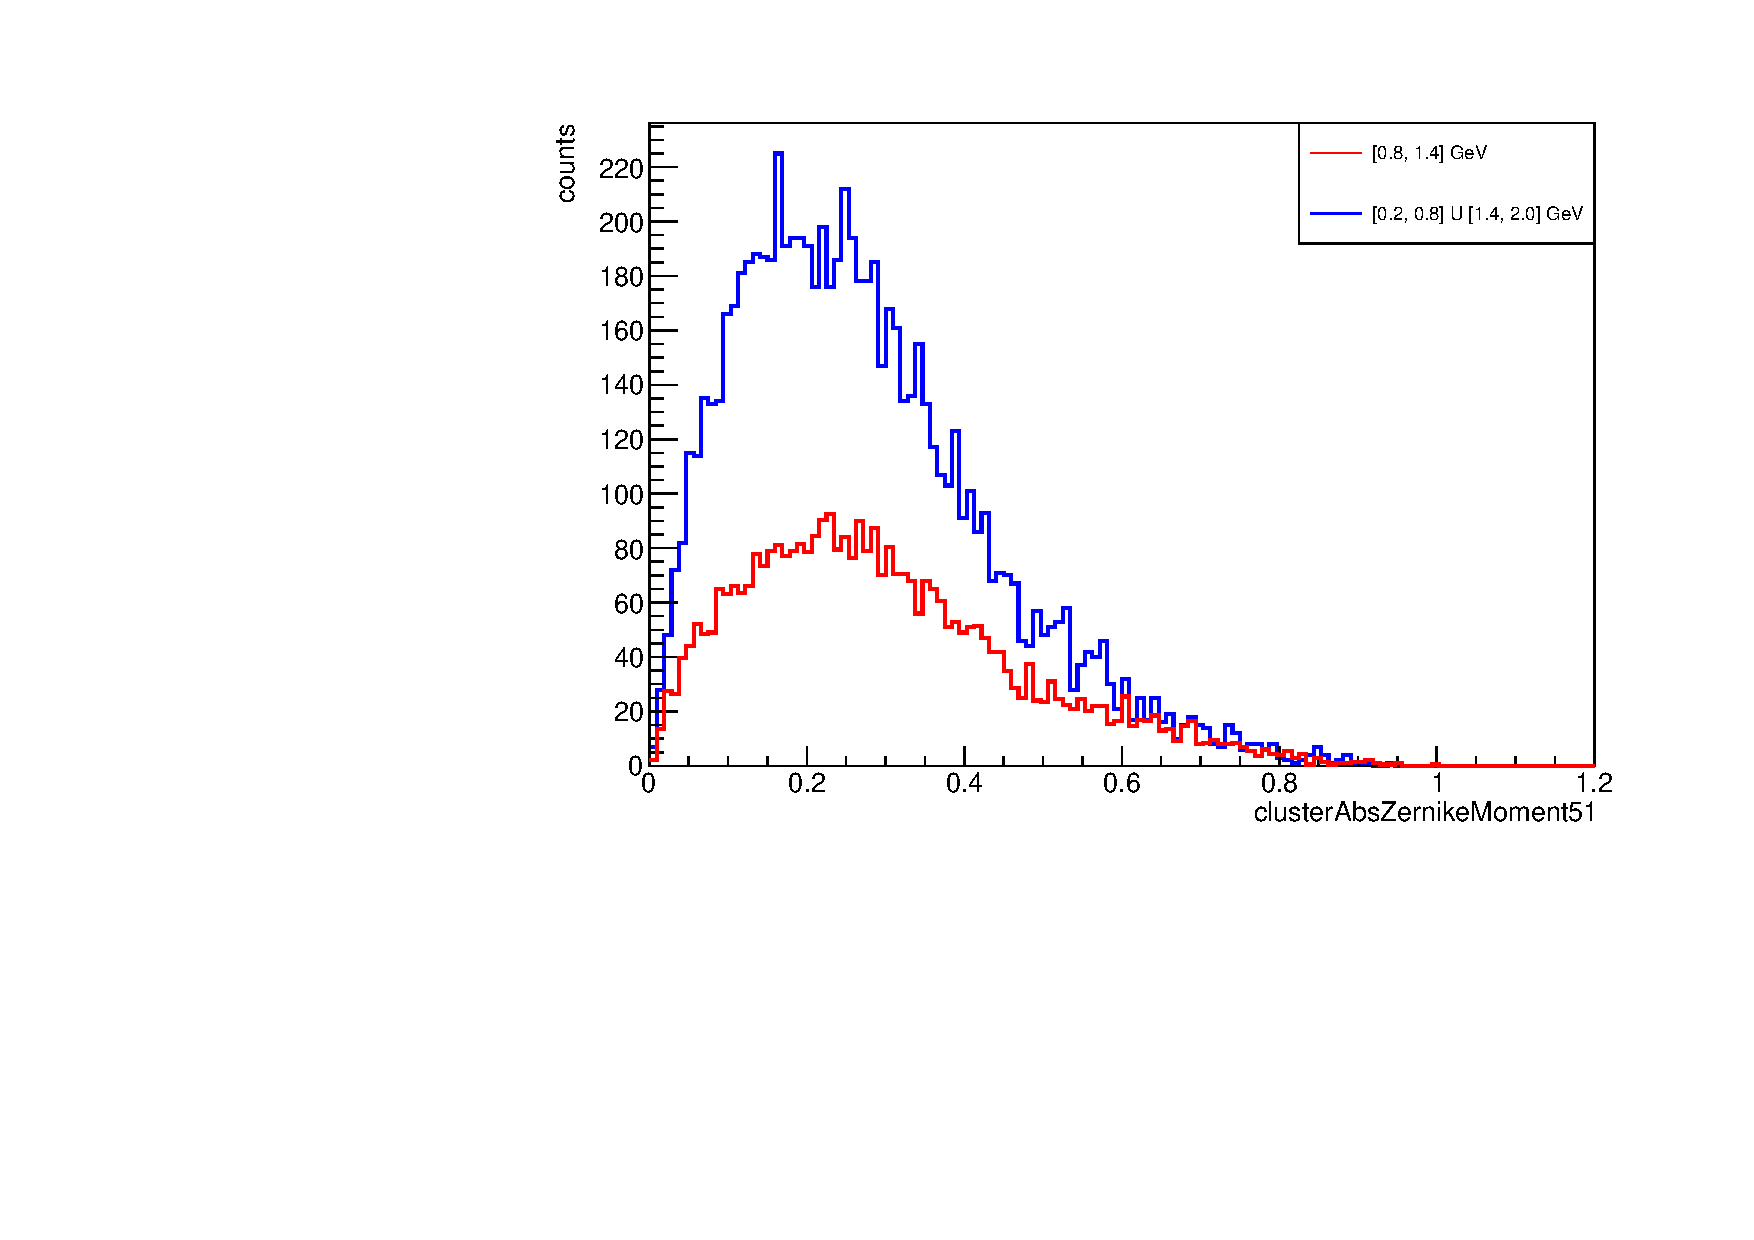
\includegraphics[width=0.49\textwidth]{nbar_cocktail/images/sidebands_clusterAbsZernikeMoment51_nog.pdf}
    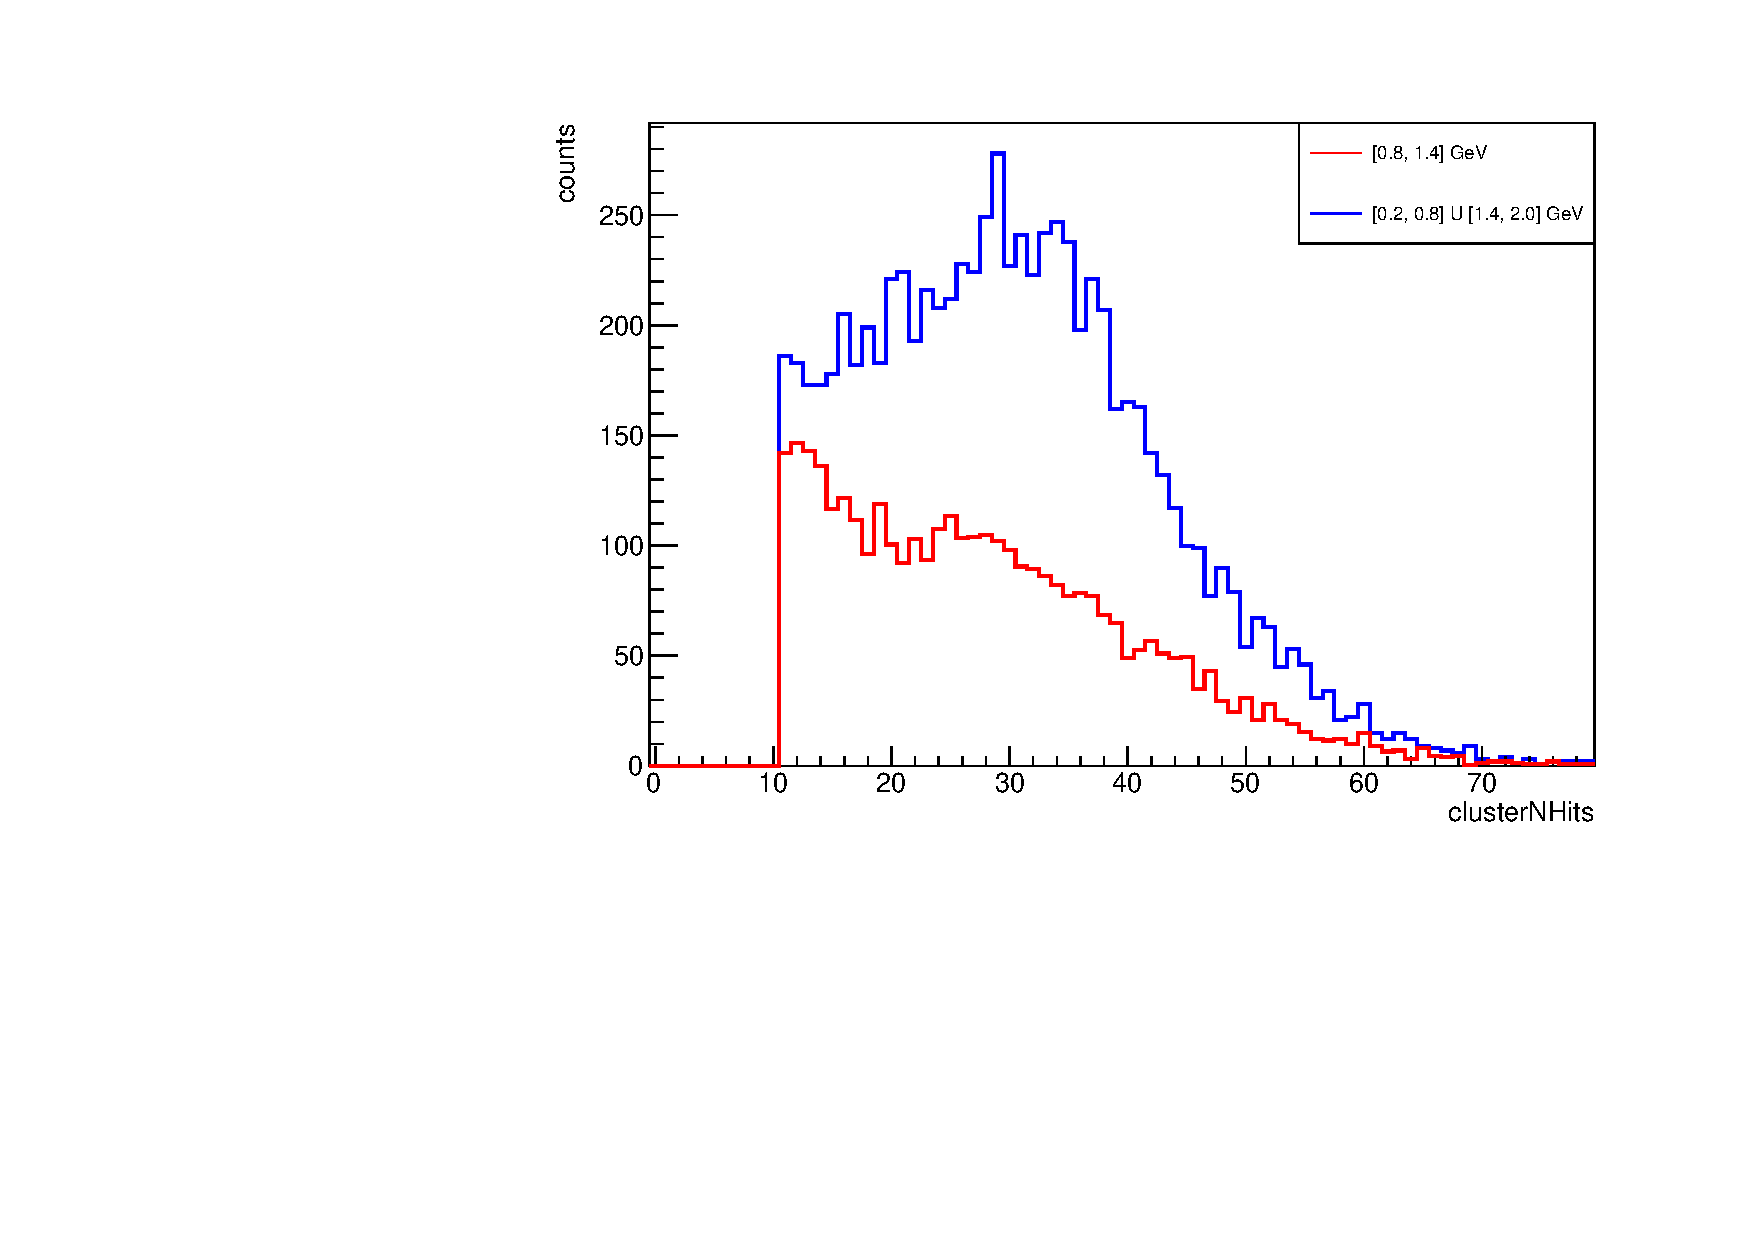
\includegraphics[width=0.49\textwidth]{nbar_cocktail/images/sidebands_clusterNHits_nog.pdf}
     \caption{Comparison of reconstructed cluster variables for $\bar{n}$ candidates in the signal region [0.8, 1.2] GeV (blue) with $\bar{n}$ candidates in the sidebands region [0.3, 0.7] U [1.3, 1.7]  GeV  (red), in NO ISR case. A scaling factor of $k = 0.5$ has been applied to the cluster variables obtained from the sidebands regions. q$\bar{q}$ cocktail.}
     \label{fig:clus_vars_sidebands_pre}
\end{figure}
$\\$
The cluster energy distribution shows a flat contribution from the sidebands regions, where no specific structure was observed. The E1E9 distribution shows that the structure observed in $\sim 0.85$ (Fig.~\ref{fig:clus_vars_nog_qqbar}) is mainly caused by background components, such as those coming from the sidebands regions. The same conclusion can be reached for the structure observed close to unity in the E9E21 distribution. 
$\\$
Furthermore, the sidebands regions provide the main contribution to the structure observed at low values in the Second Moment distribution, caused by small-sized clusters. 
$\\$
The cluster Zernike moment $Z^0_4$ presents a tail around $Z^0_4 \sim 1.2$ caused by sidebands contribution, while $Z^1_5$ presents no discernible structure.
$\\$
Afterwards, the structure observed at a value of $\sim 0.3$ in the Lateral Momentum distribution is caused by sidebands contribution.
$\\$
Therefore, to obtain the final $\bar{n}$ candidates cluster variables distribution, the sidebands regions contribution (background) is subtracted from the signal region contribution (signal + background). The obtained cluster variables are shown in Fig.\ref{fig:clus_vars_sidebands_post}.

 \begin{figure}[h]
    \centering
    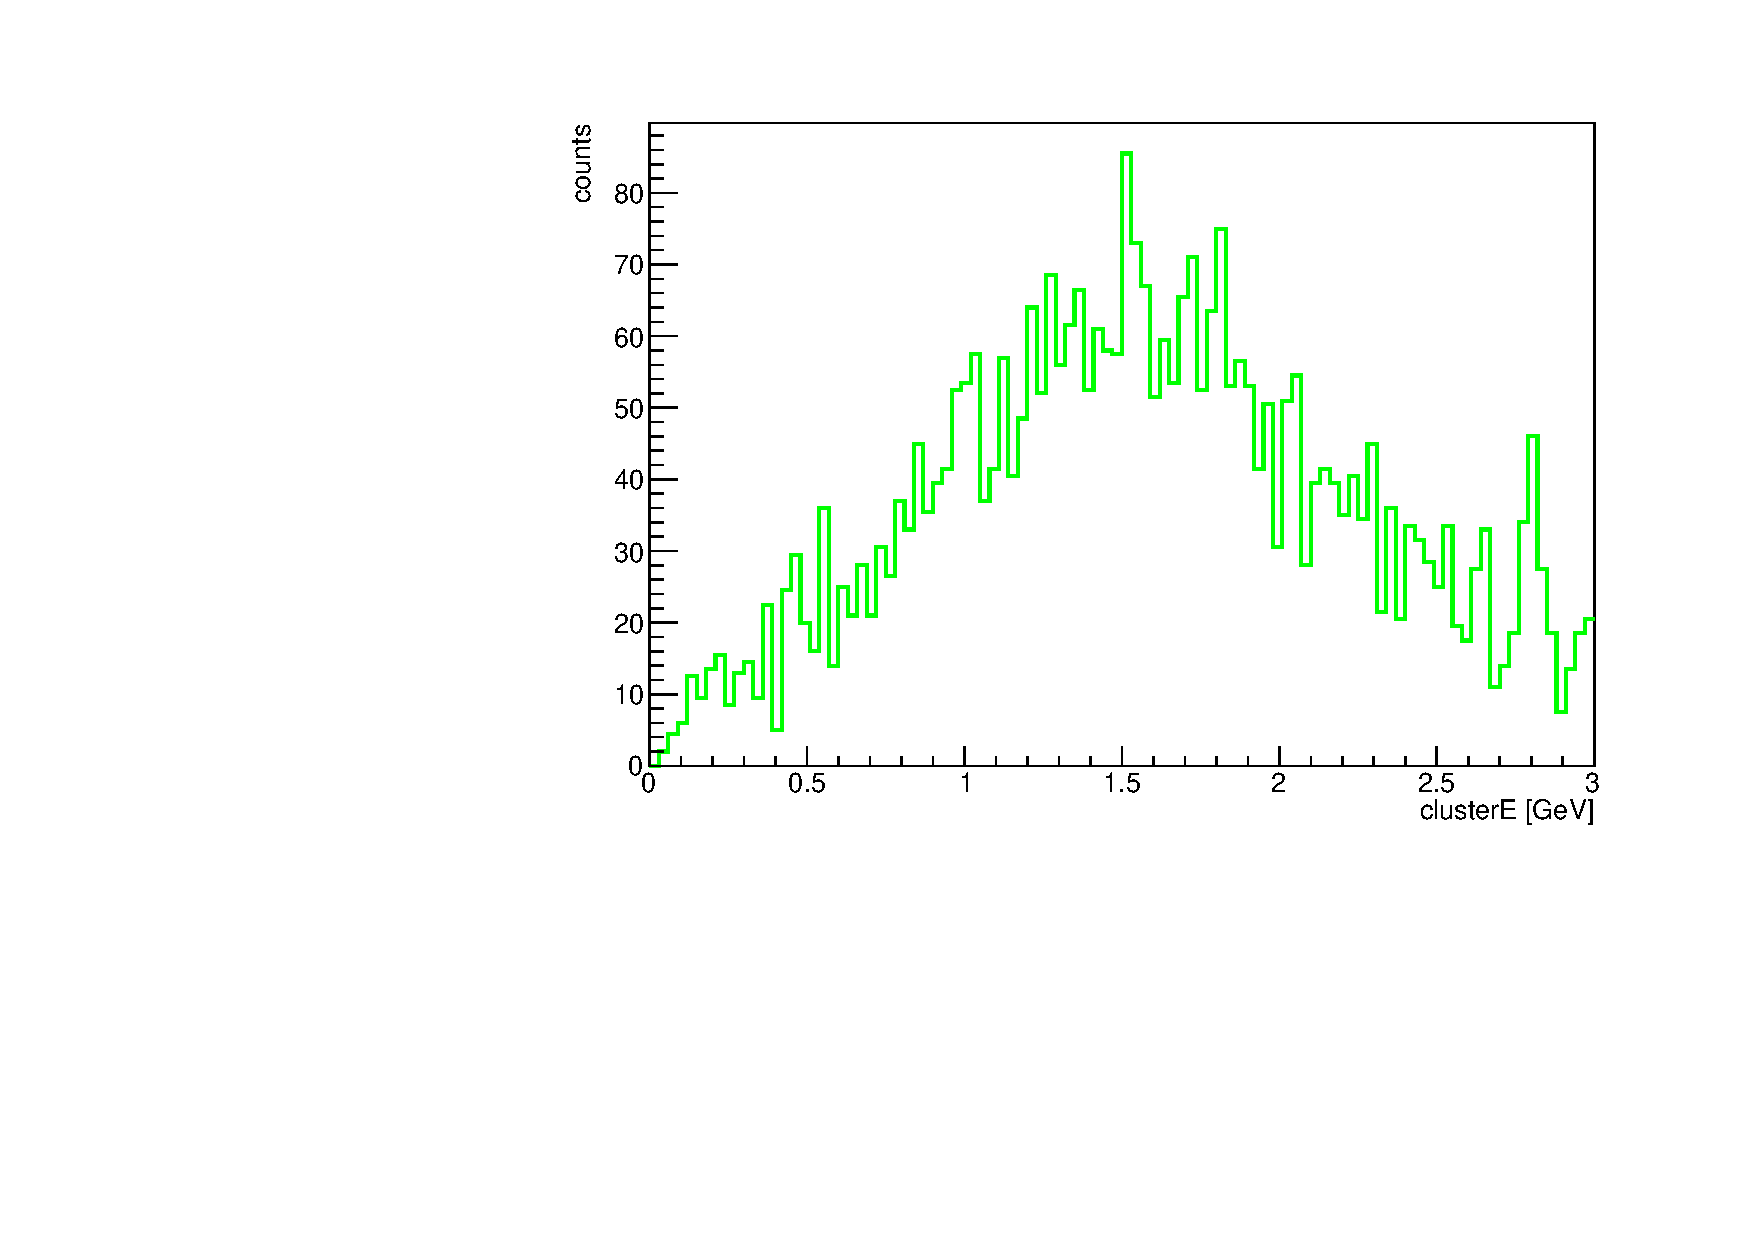
\includegraphics[width=0.49\textwidth]{nbar_cocktail/images/final_clusterE_nog.pdf}
    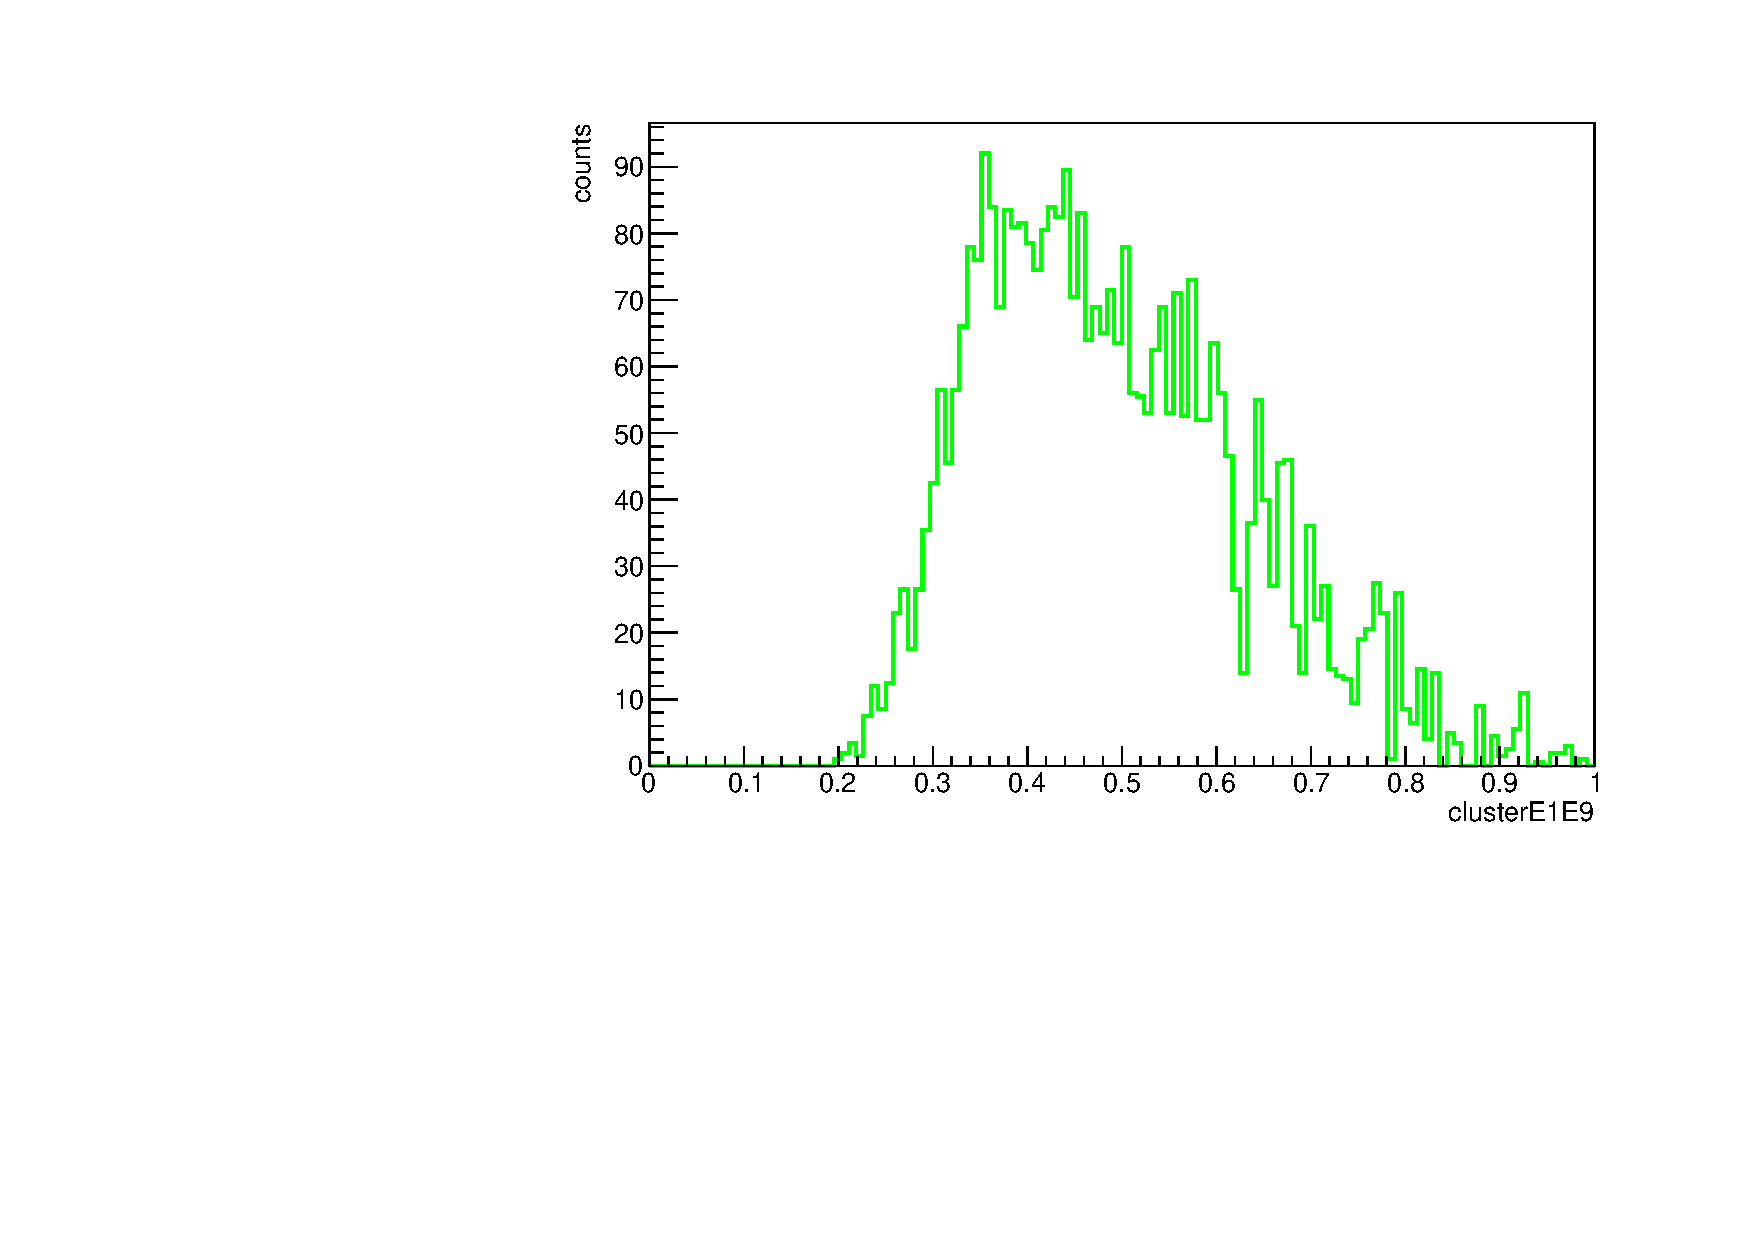
\includegraphics[width=0.49\textwidth]{nbar_cocktail/images/final_clusterE1E9_nog.pdf}
    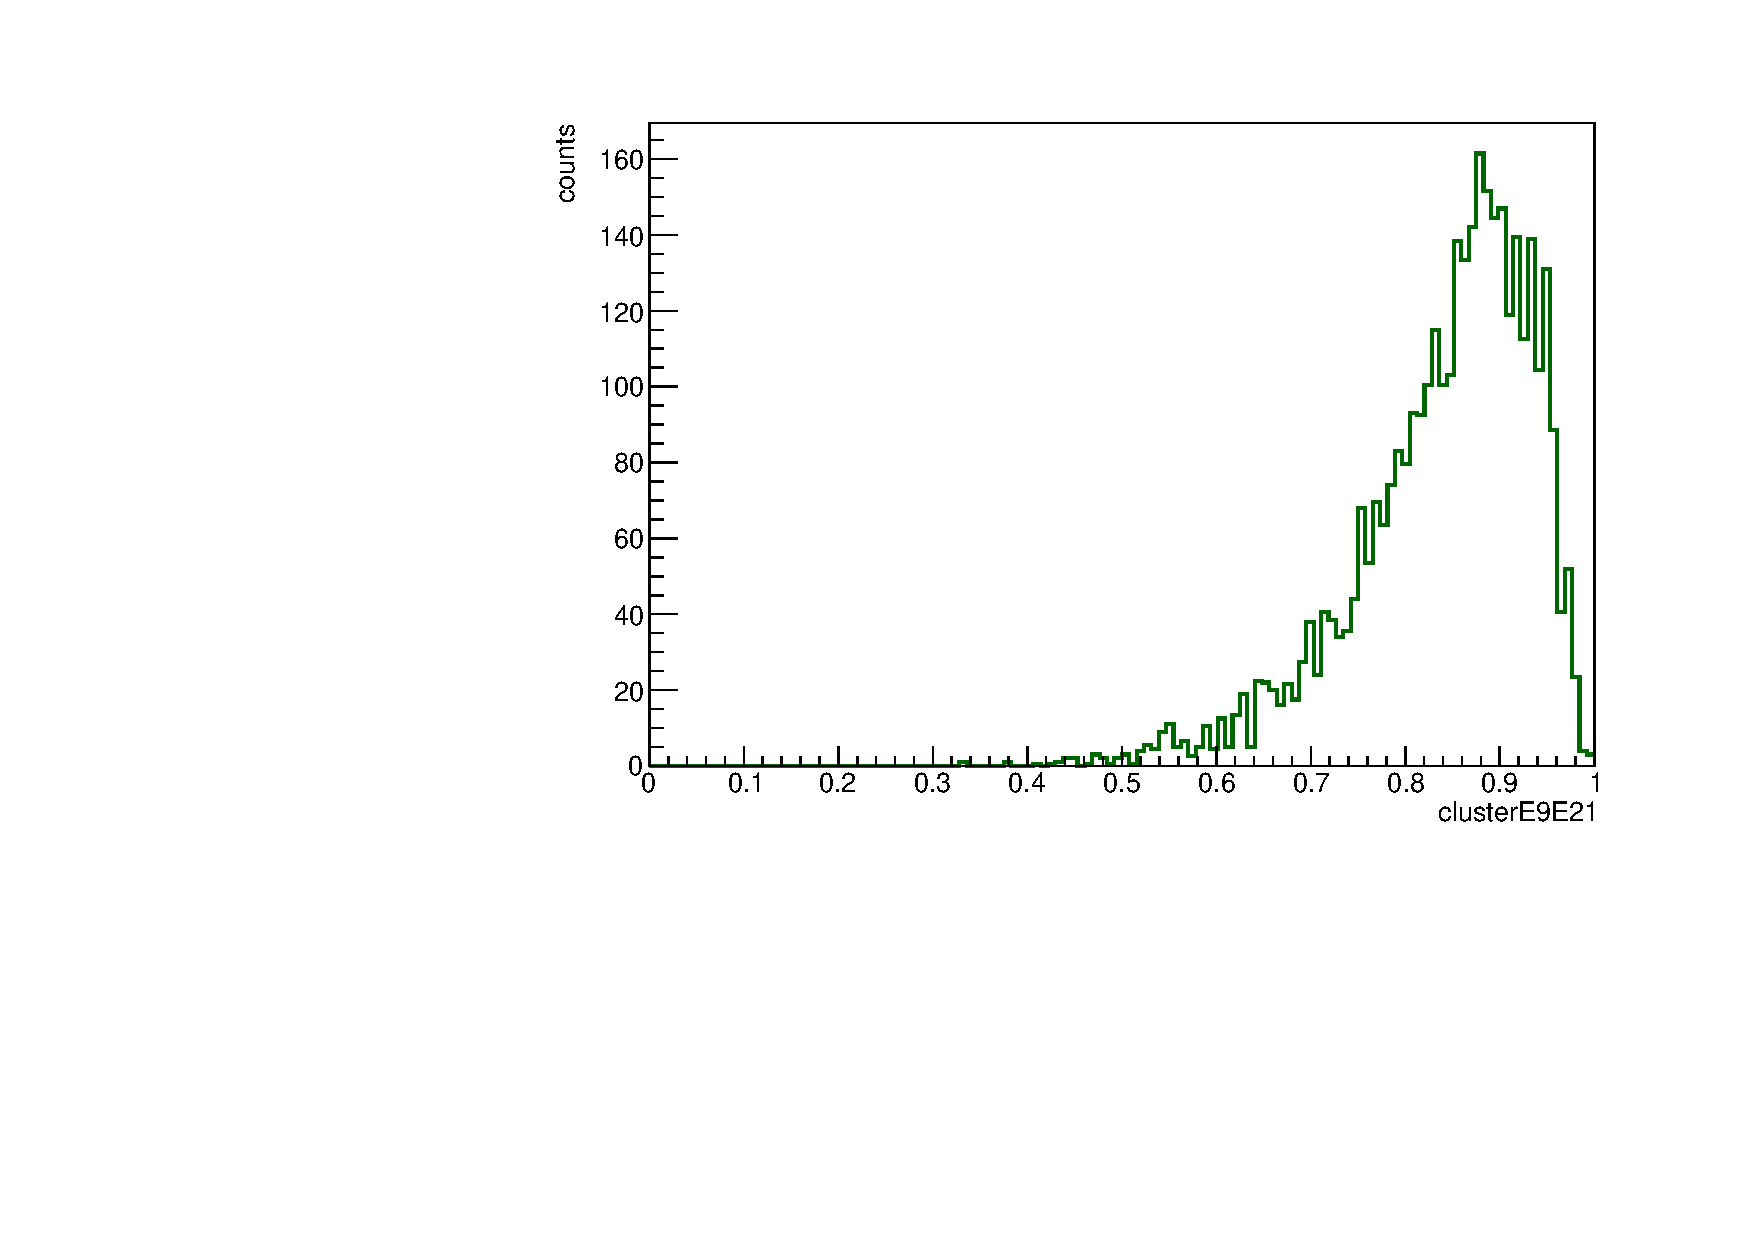
\includegraphics[width=0.49\textwidth]{nbar_cocktail/images/final_clusterE9E21_nog.pdf}
    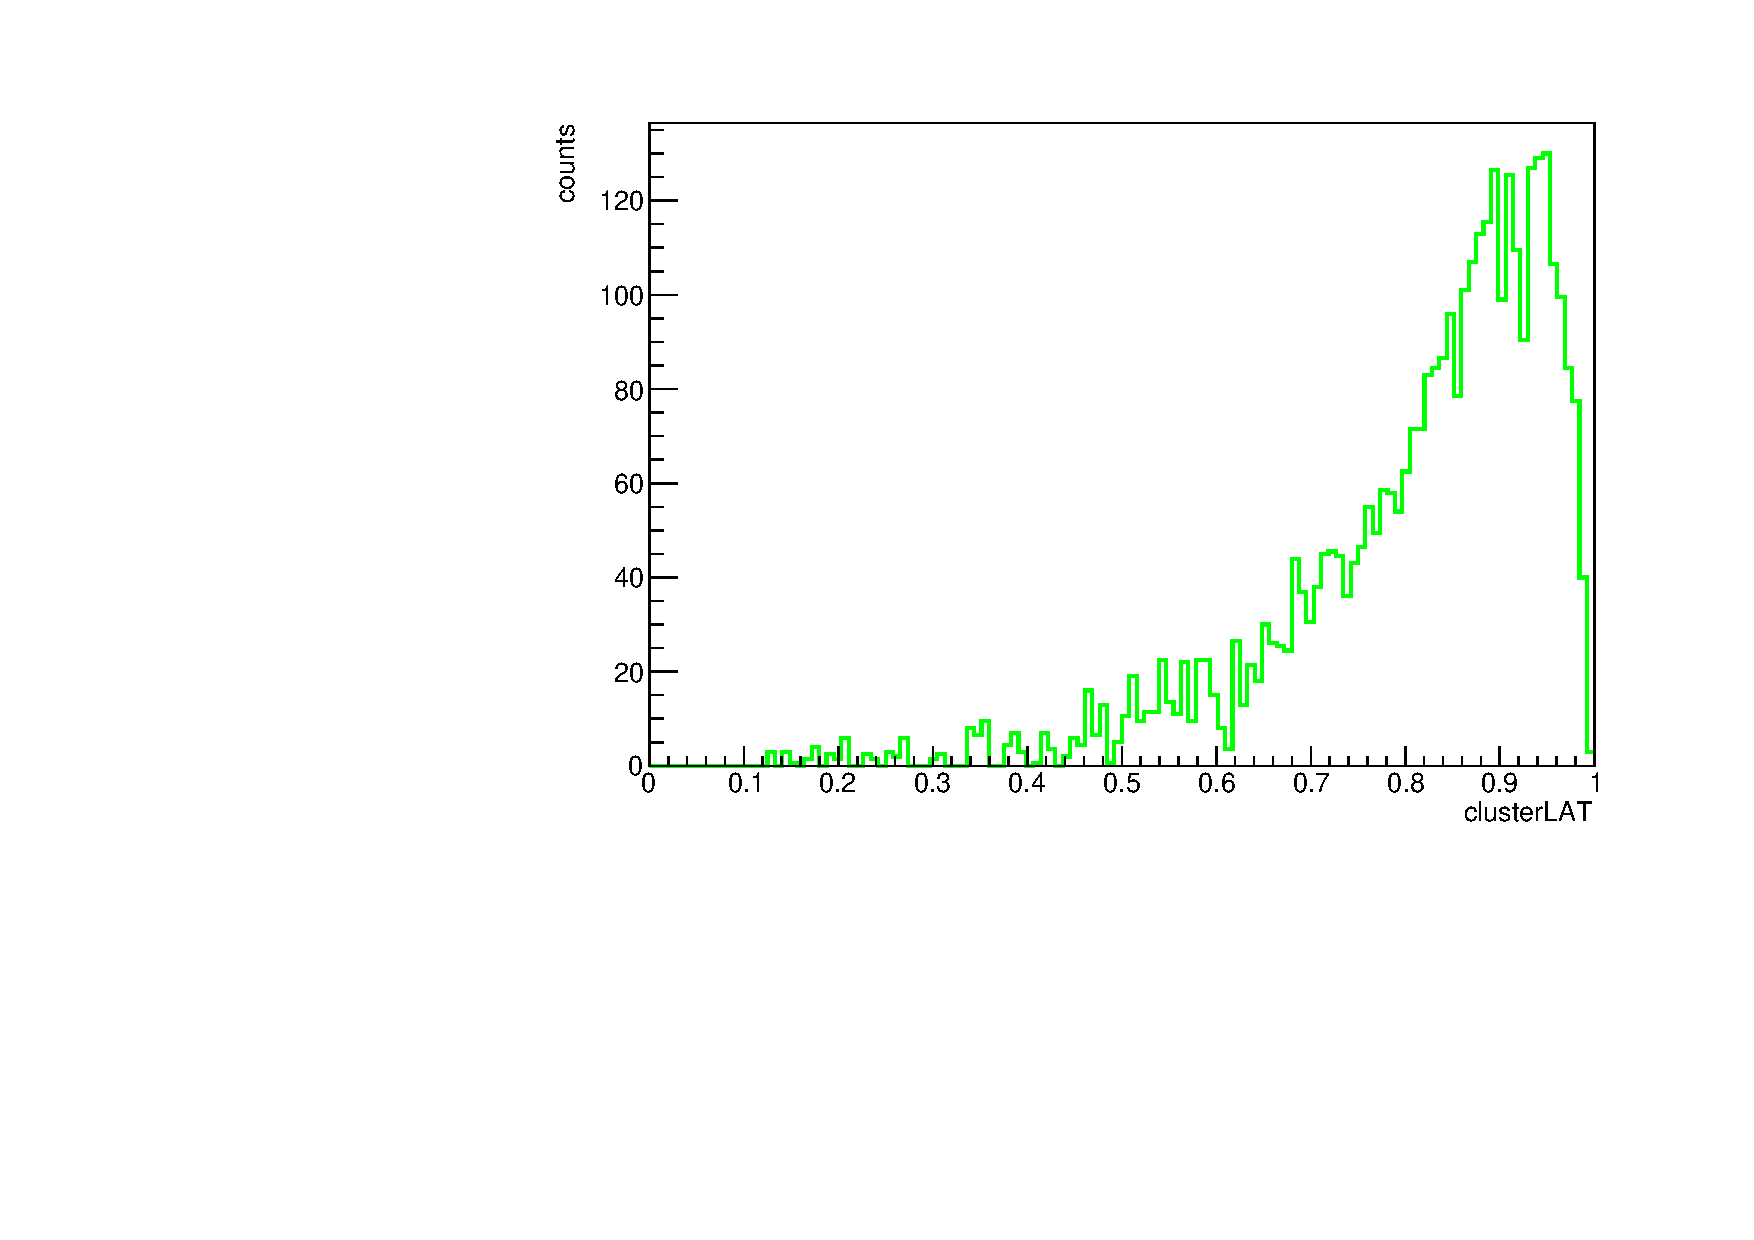
\includegraphics[width=0.49\textwidth]{nbar_cocktail/images/final_clusterLAT_nog.pdf}
    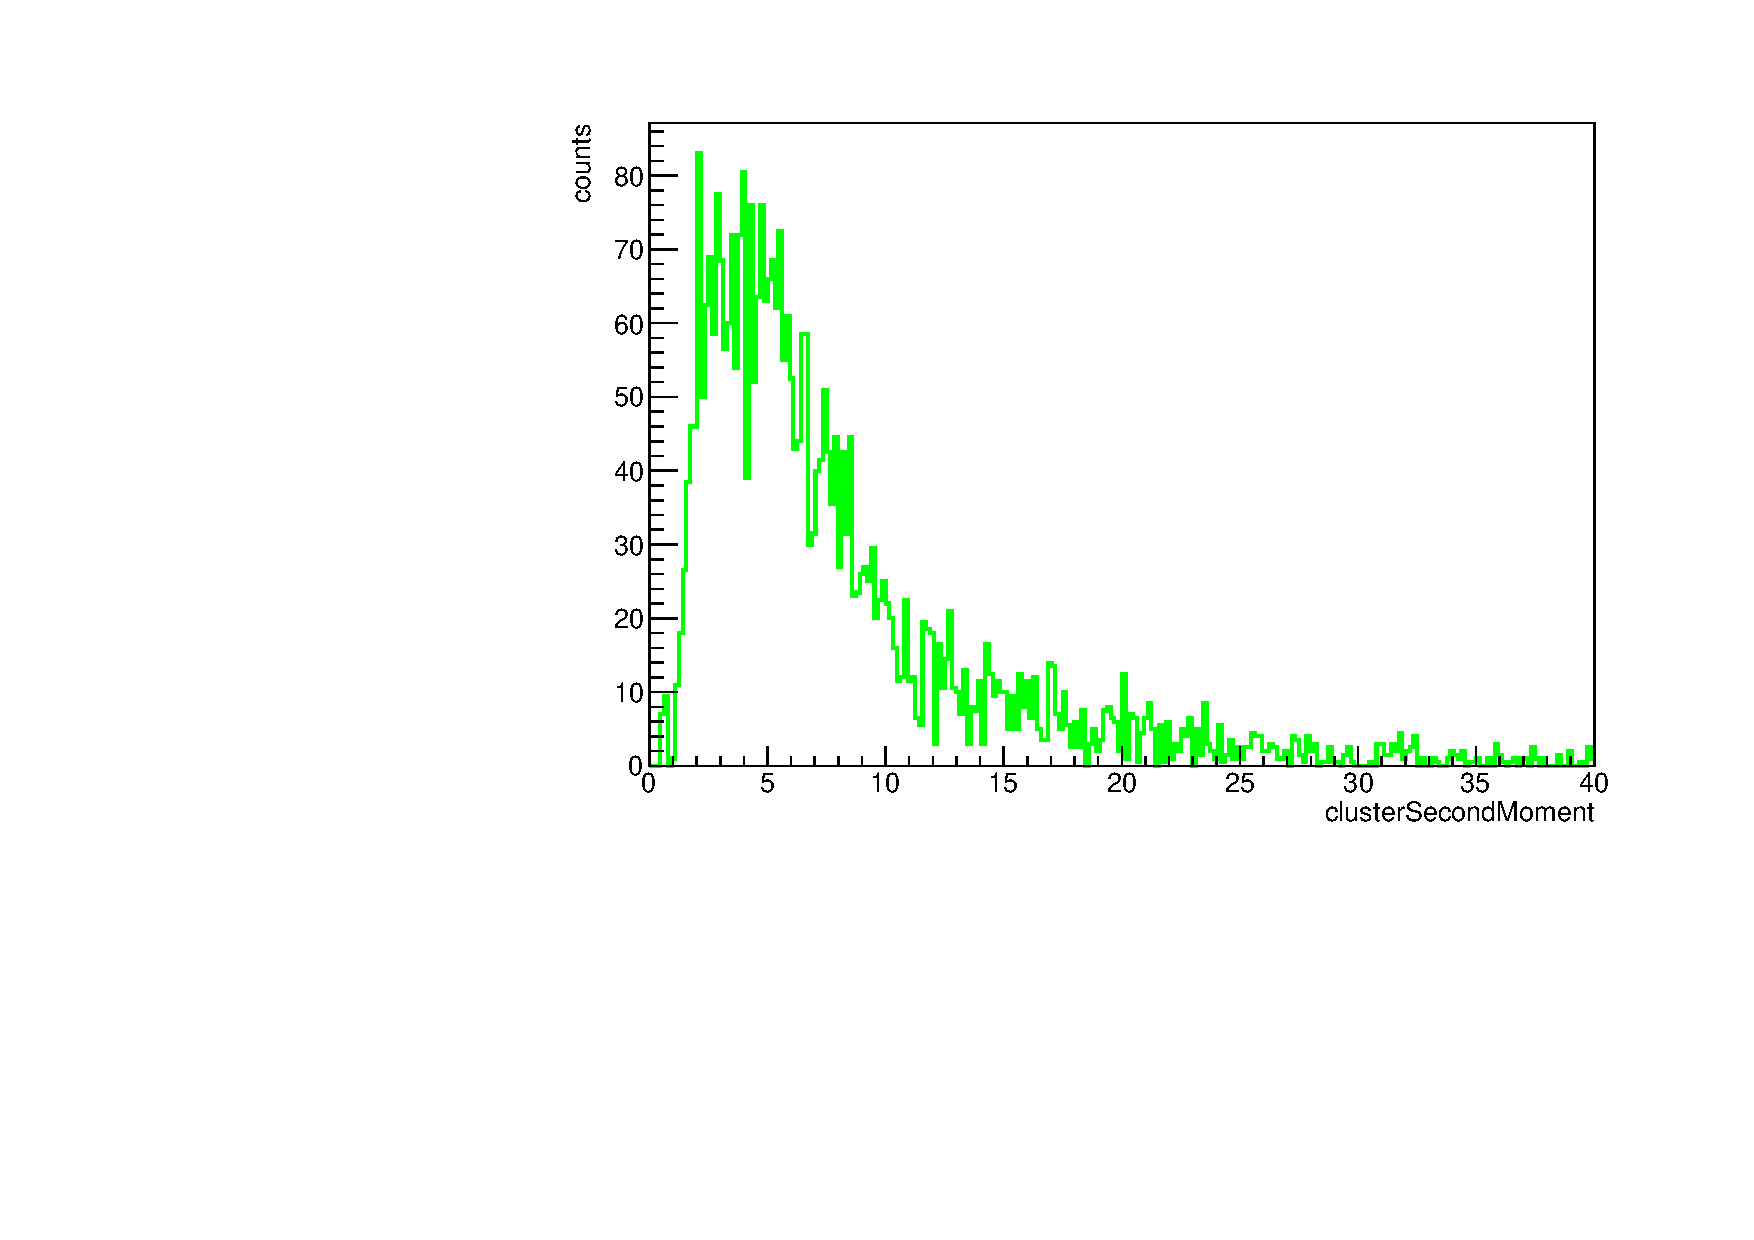
\includegraphics[width=0.49\textwidth]{nbar_cocktail/images/final_clusterSecondMoment_nog.pdf}
    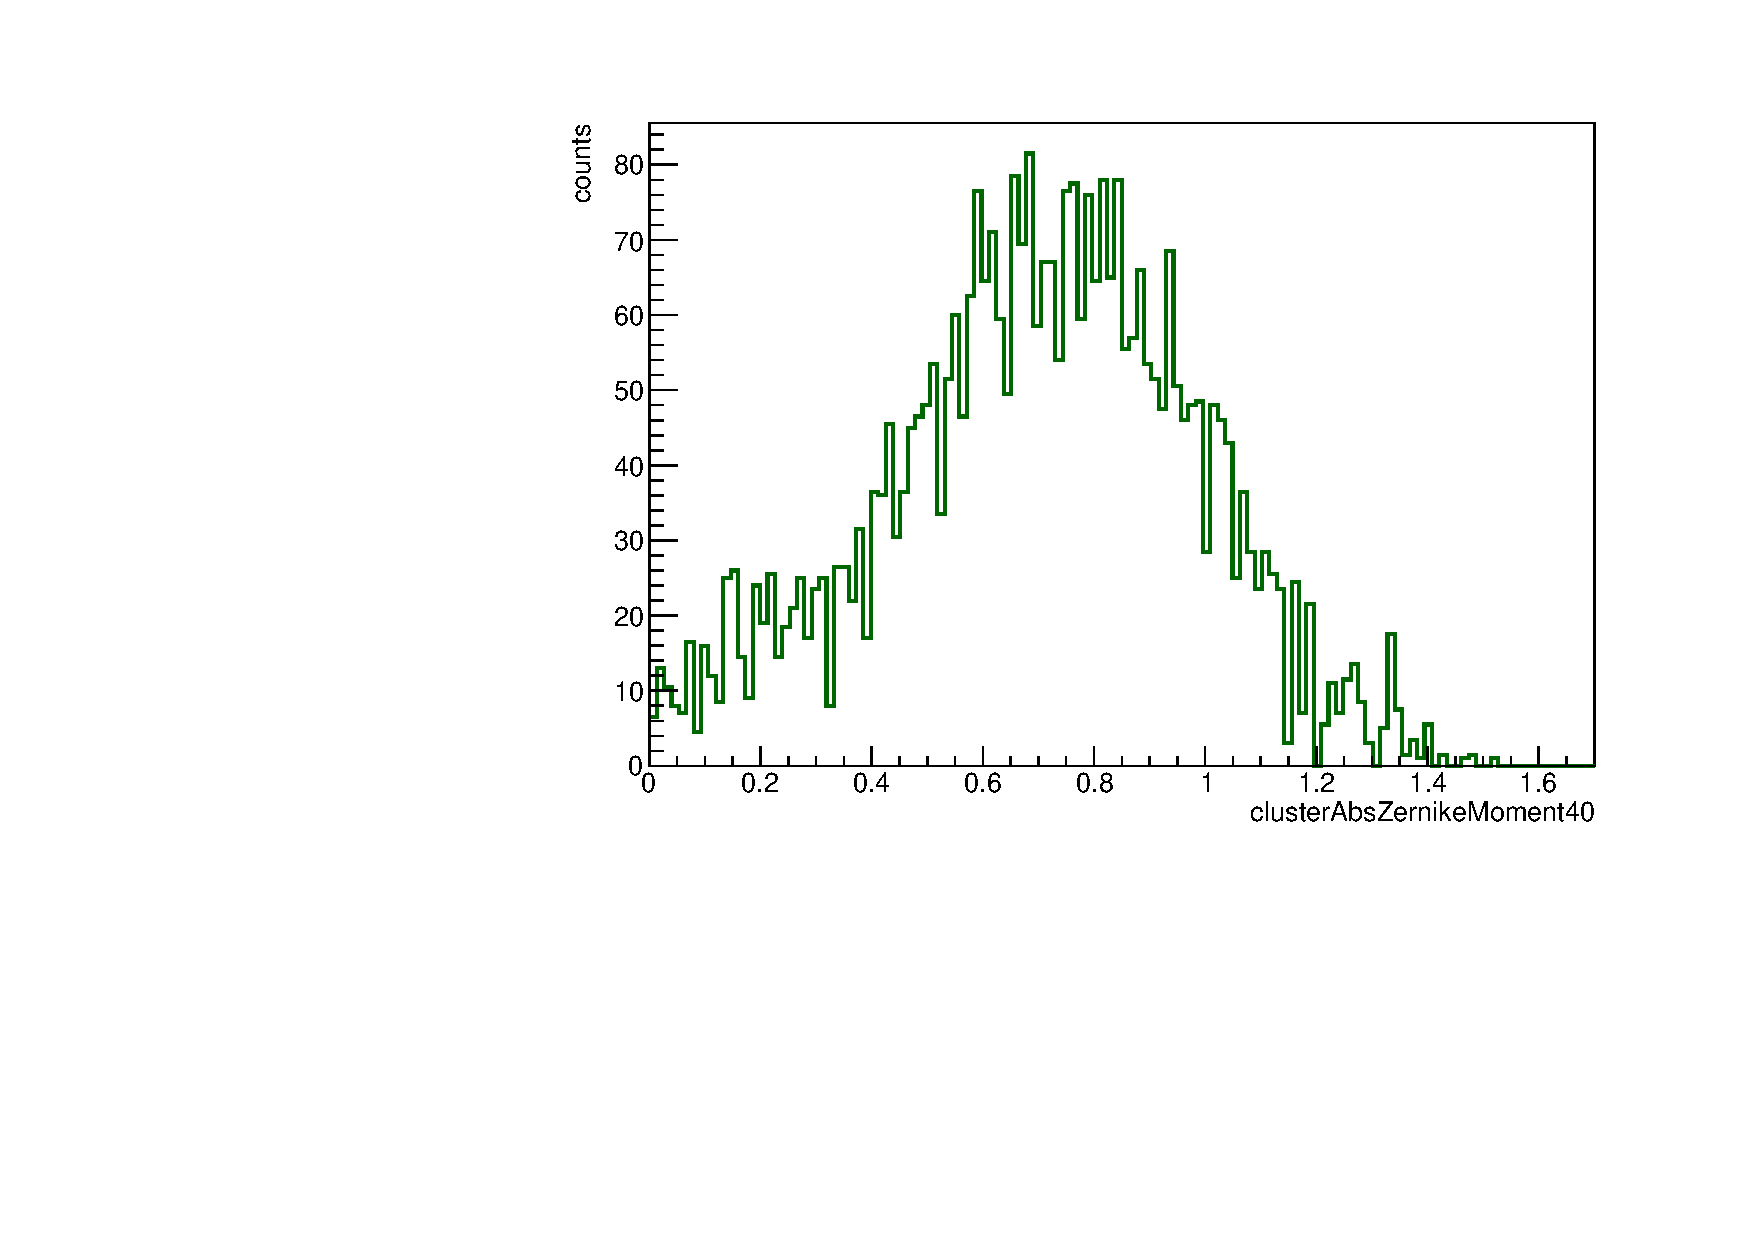
\includegraphics[width=0.49\textwidth]{nbar_cocktail/images/final_clusterAbsZernikeMoment40_nog.pdf}
    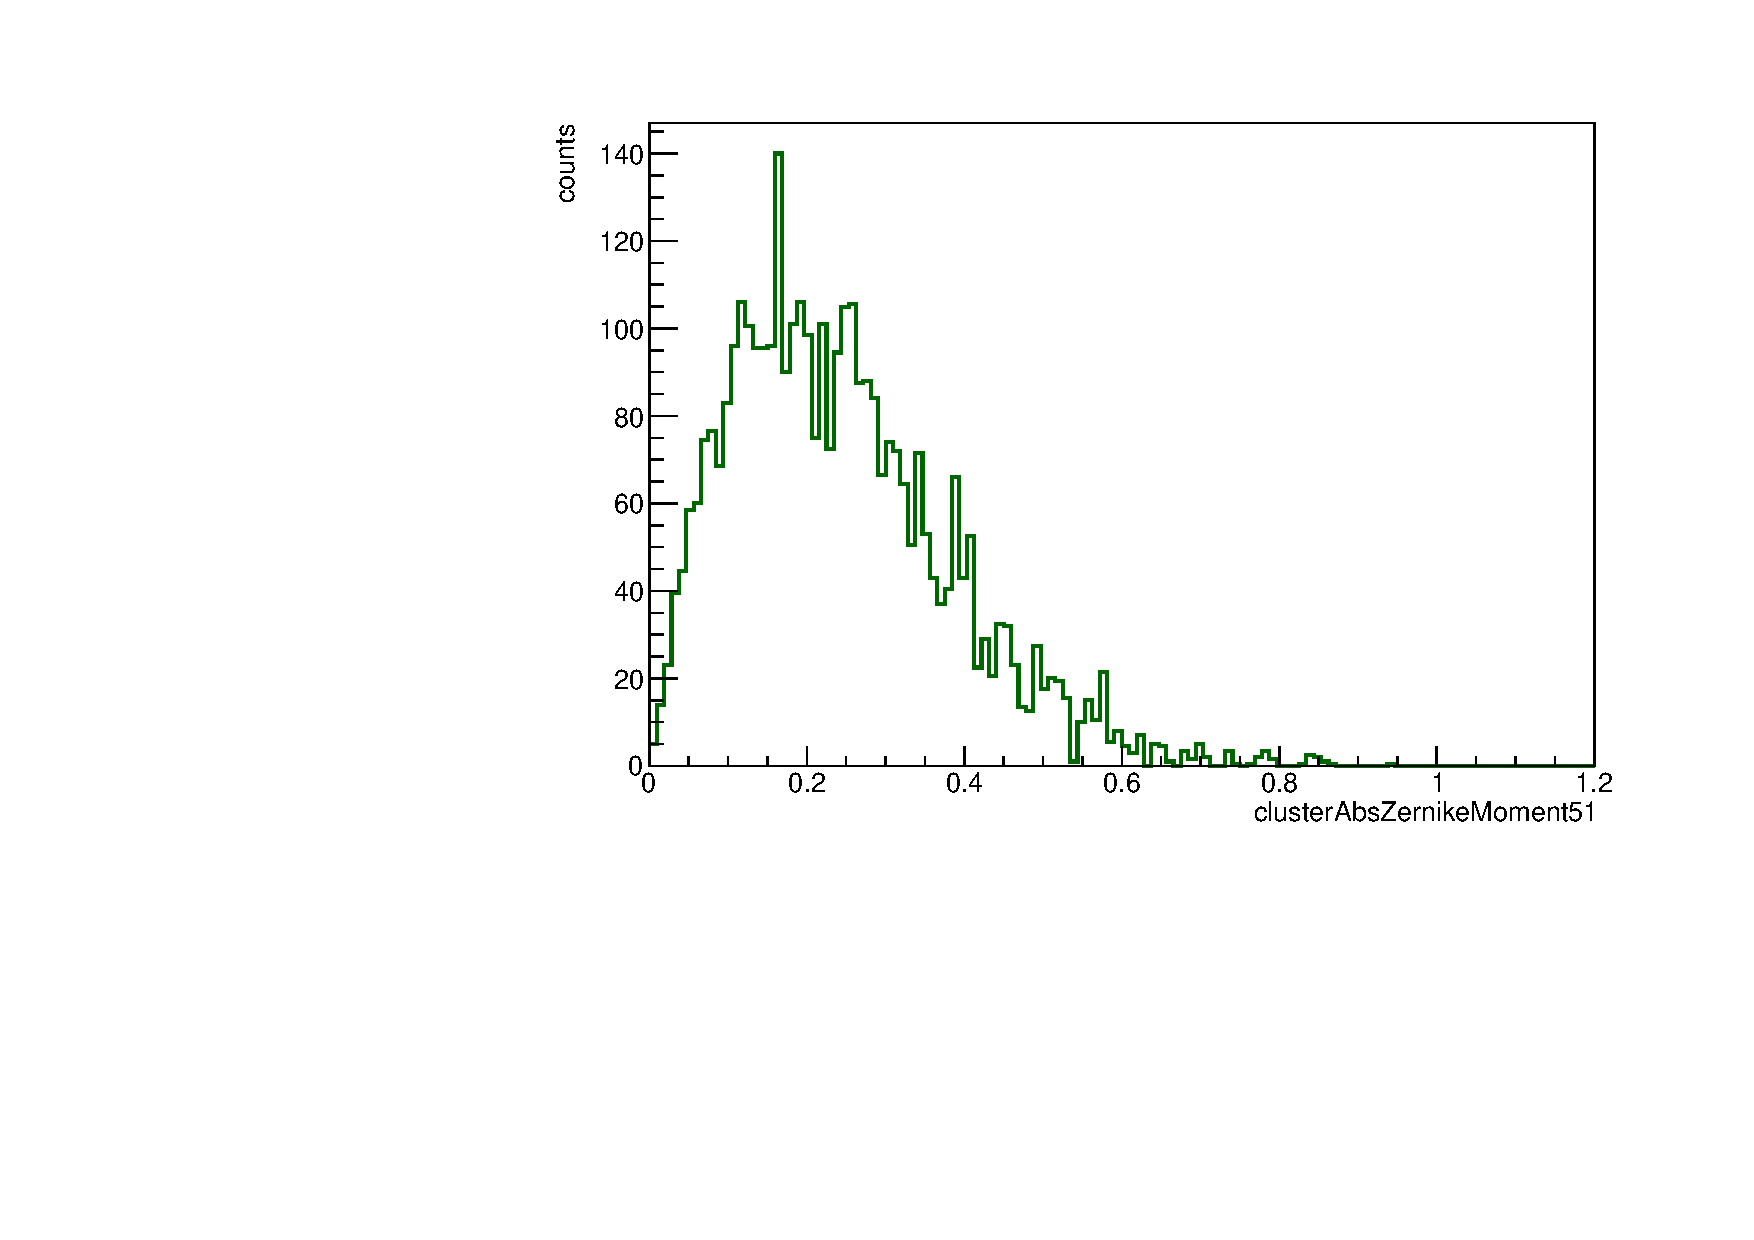
\includegraphics[width=0.49\textwidth]{nbar_cocktail/images/final_clusterAbsZernikeMoment51_nog.pdf}
    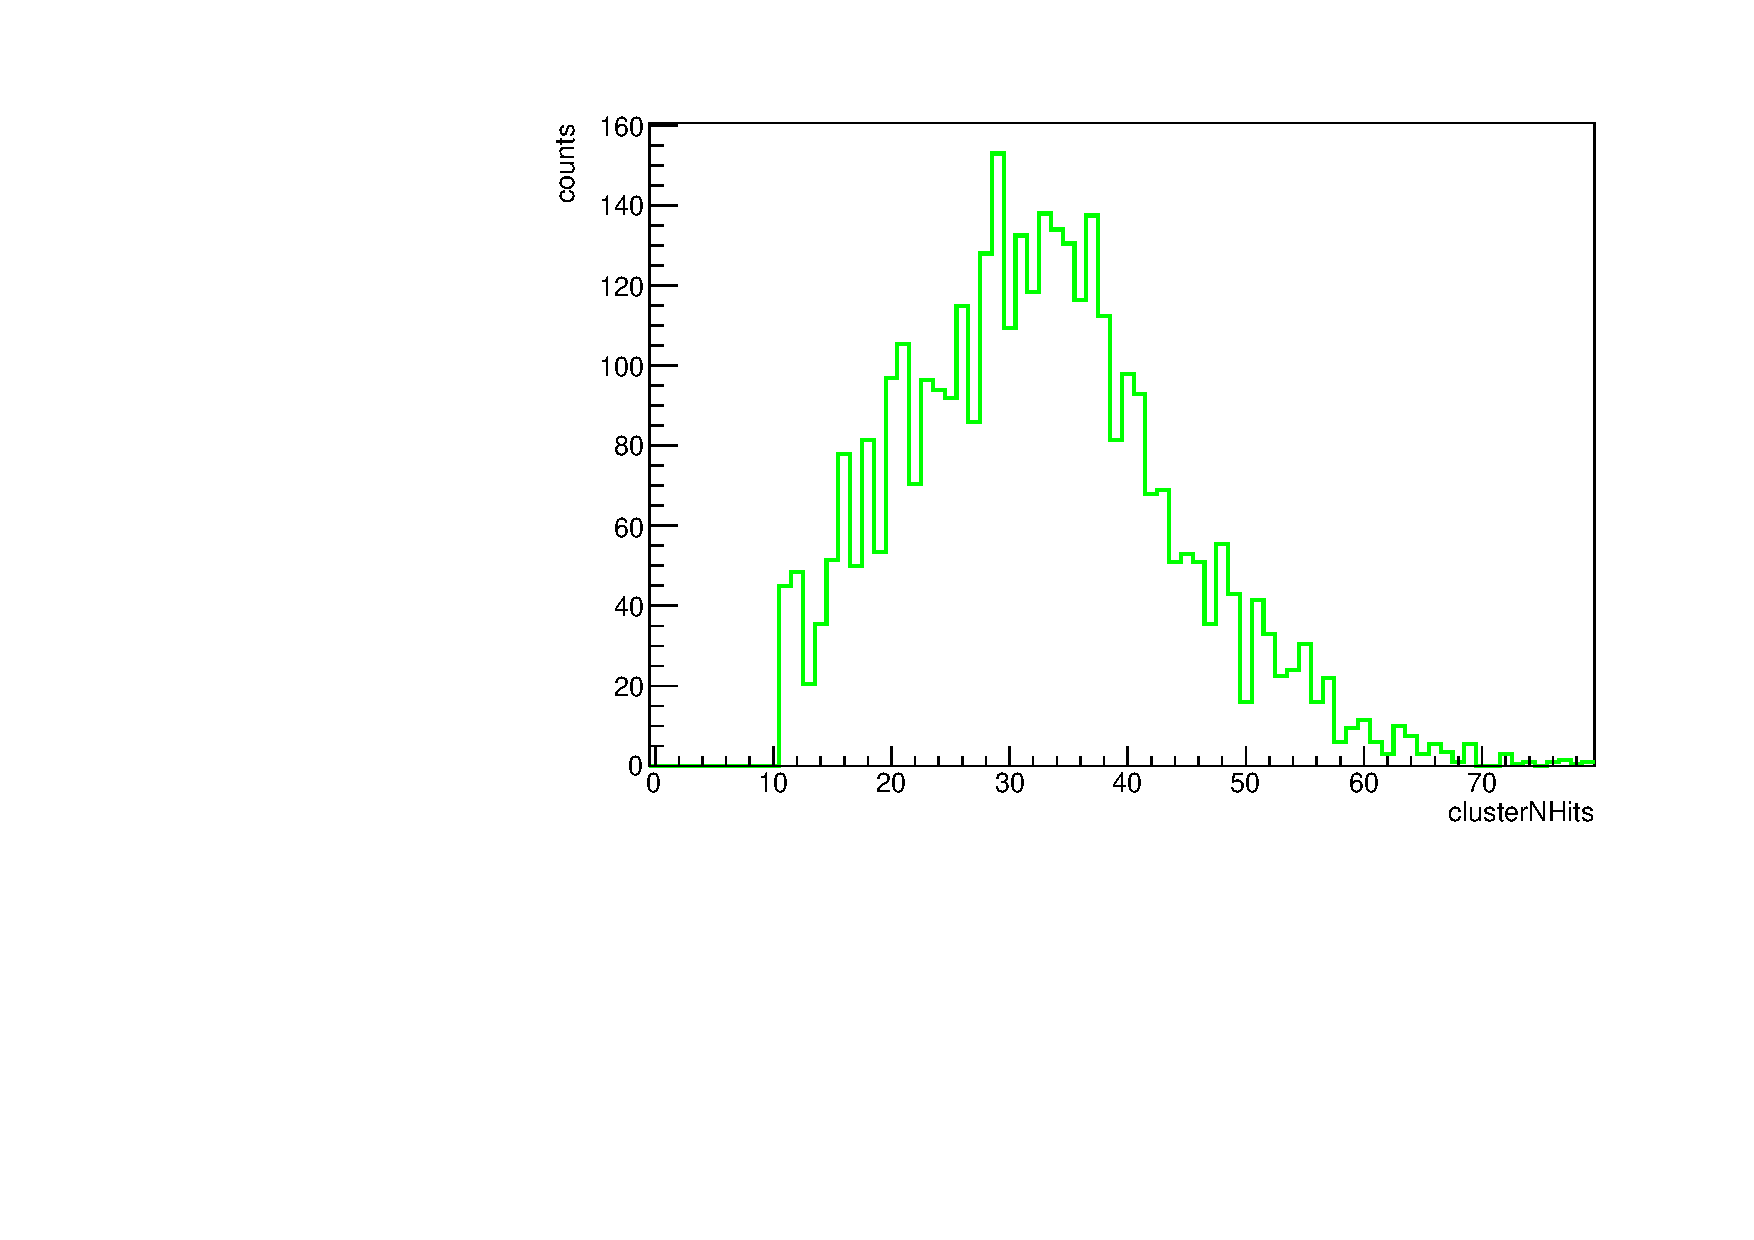
\includegraphics[width=0.49\textwidth]{nbar_cocktail/images/final_clusterNHits_nog.pdf}
   
     \caption{Reconstructed cluster variables for $\bar{n}$ candidates after the application of the sidebands technique, in NO ISR case. q$\bar{q}$ cocktail.}
     \label{fig:clus_vars_sidebands_post}
\end{figure}

The obtained cluster variables distributions no longer present the singular structures observed prior to the sidebands technique application. This leads to reconstructed cluster variables more similar to those obtained from the Monte Carlo signal sample analysis (Fig.~\ref{fig:clus_vars_2}). This suggests that the applied selections and the sidebands technique properly separate the signal contribution from the background one, in q$\bar{q}$ cocktail, with no explicit $\gamma_{ISR}$ reconstruction.

\subsection{$q\bar{q}$ cocktail production (ISR case)}
Since the same path as the NO ISR case has been followed, in the ISR case the $q\bar{q}$ cocktail is directly analyzed. The same final selections adopted in the NO ISR case have been used.
$\\$
The TopoAna output of can be consulted in Fig.~\ref{fig:topo_isr_010_qqbar}.
\begin{figure}[H]
    \centering
    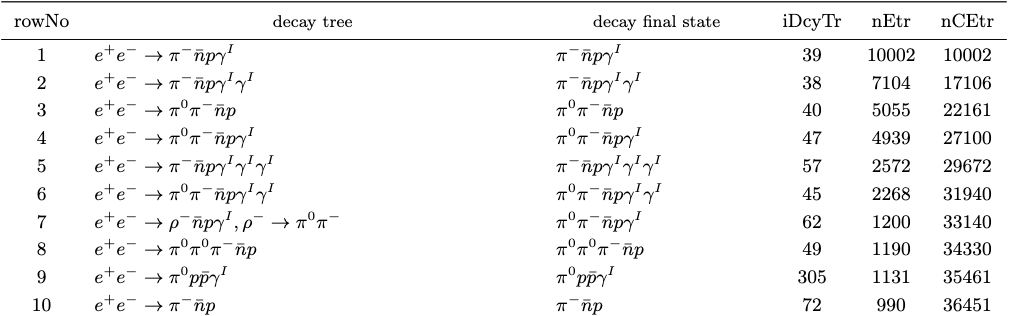
\includegraphics[width=1\textwidth]{nbar_cocktail/images/topoana_isr_010_qqbar}
    \caption{First 10 channels of the TopoAna output in $q\bar{q}$ Monte Carlo cocktail, showing the different channel contributes. ISR case.}
    \label{fig:topo_isr_010_qqbar}
\end{figure}
The TopoAna output reveals a situation very similar to that obtained in the NO ISR case. In fact, now, the dominant contribution is from the signal channel $p \pi^- \bar{n} \gamma_{ISR}$. A secondary contribution comes from $p \pi^- \bar{n} \gamma_{ISR}  \gamma_{ISR}$, which could be treated as signal despite the extra $\gamma_{\text{ISR}}$ not being explicitly reconstructed. The next contribution comes from $p \pi^- \bar{n} \pi^0$ in the final state. The fourth contribution is due to $p \pi^- \bar{n} \pi^0 \gamma_{\text{ISR}}$, and so on. The individual TopoAna outputs from $u\bar{u}$, $d\bar{d}$, $s\bar{s}$ and $c\bar{c}$ are shown in Fig.~\ref{fig:topo_isr_010_qqbar_singles}.
\begin{figure}[H]
    \centering
    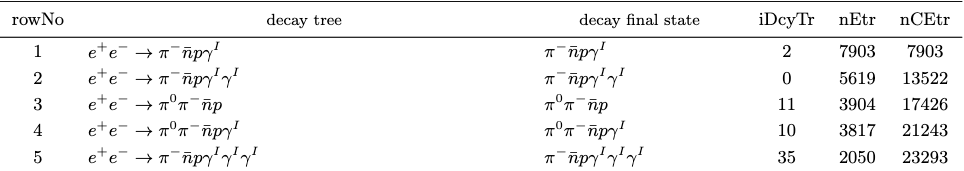
\includegraphics[width=1\textwidth]{nbar_cocktail/images/topo_uubar_isr}
    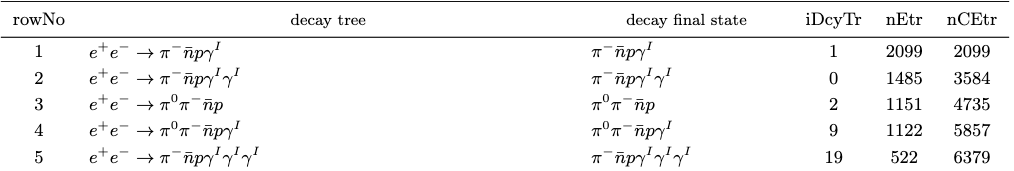
\includegraphics[width=1\textwidth]{nbar_cocktail/images/topo_ddbar_isr}
    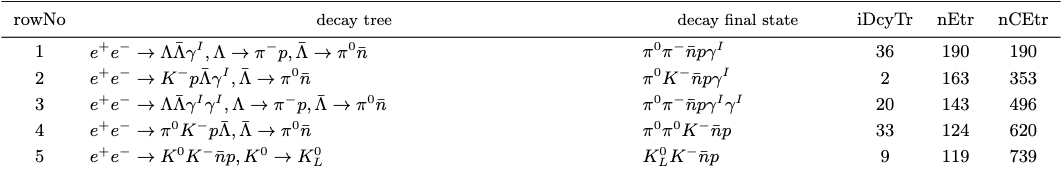
\includegraphics[width=1\textwidth]{nbar_cocktail/images/topo_ssbar_isr}
    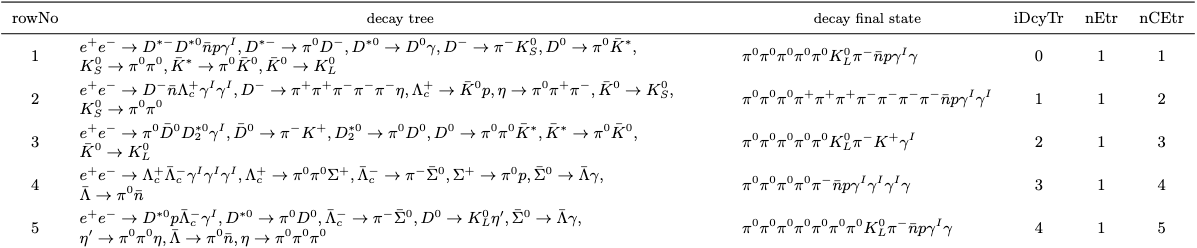
\includegraphics[width=1\textwidth]{nbar_cocktail/images/topo_ccbar_isr}
    \caption{Top 5 channels from the TopoAna output respectively for the $u\bar{u}$, $d\bar{d}$, $s\bar{s}$, and $c\bar{c}$ Monte Carlo cocktails (from top to bottom). ISR case.}
    \label{fig:topo_isr_010_qqbar_singles}
\end{figure}
As observed in the NO ISR case, the main contributions to the final signal state are from the $u\bar{u}$ and $d\bar{d}$ cocktails in the ISR case as well. The obtained stacked components to the recoil mass, in $q\bar{q}$ cocktail, are shown in figure ~\ref{fig:mRecComps_isr_010_qqbar}.
\begin{figure}[H]
    \centering
    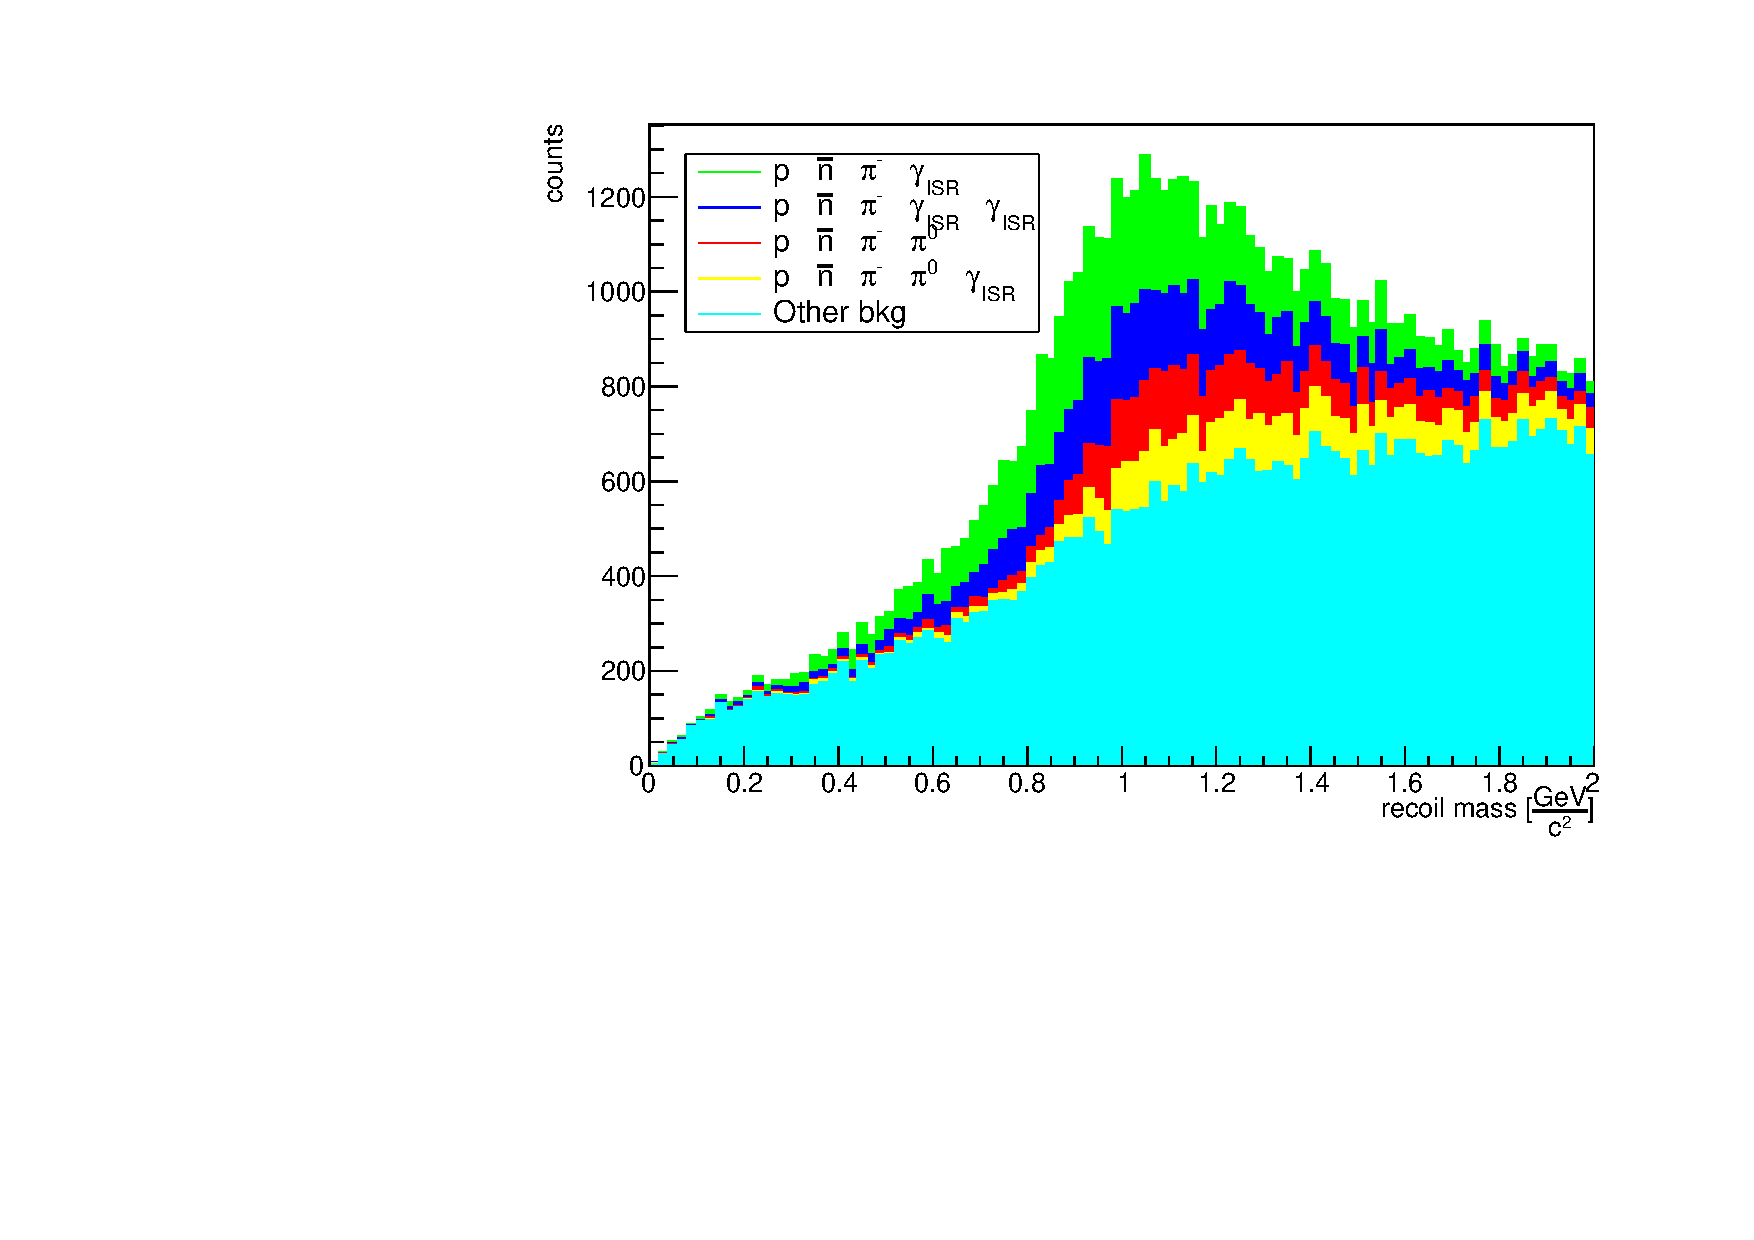
\includegraphics[width=0.8\textwidth]{nbar_cocktail/images/recoilM_qqbar_comps_isr_010}
    \caption{$p, \pi^-$ recoil mass distribution in $q\bar{q}$ Monte Carlo cocktail, displaying each stacked component contribution, ISR case. Green: $\pi^- \bar{n} p \gamma_{ISR}$ channel. Blue: $\pi^- \bar{n} p \gamma_{ISR}$ channel. Red: $\pi^0 \pi^- \bar{n} p$. Yellow: $\pi^0 \pi^- \bar{n} p \gamma_{ISR}$ channel. Cyan: other channels. $\alpha<$ 10 rad cut is applied.}
    \label{fig:mRecComps_isr_010_qqbar}
\end{figure}

No discernible contributions can be observed, as each channel contributes uniformly across the recoil mass distribution, both inside and outside the signal region [0.8, 1.2] GeV. The obtained $\bar{n}$ candidates reconstructed cluster variables are shown in Fig.\ref{fig:clus_vars_nog_qqbar}. 
 \begin{figure}[h]
    \centering
    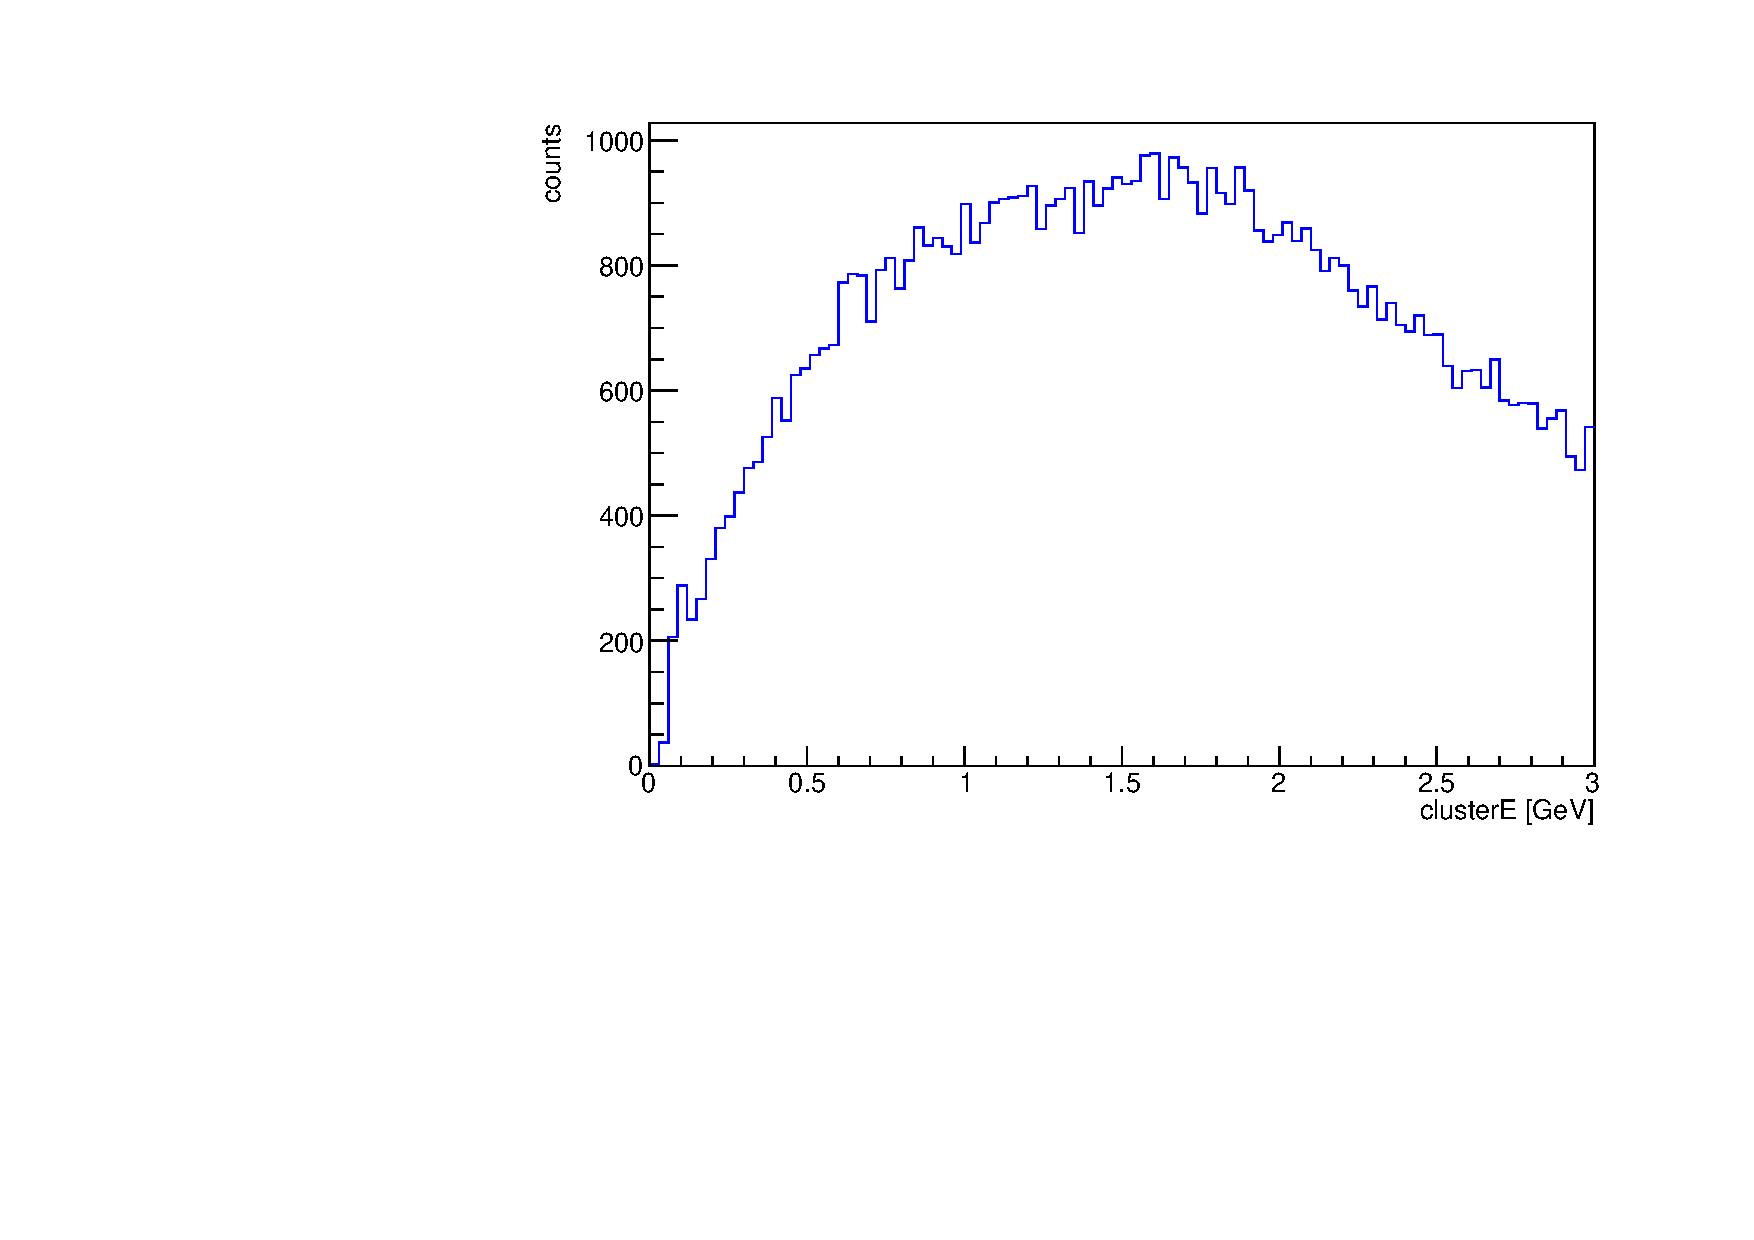
\includegraphics[width=0.49\textwidth]{nbar_cocktail/images/clusterE_isr_qqbar.pdf}
    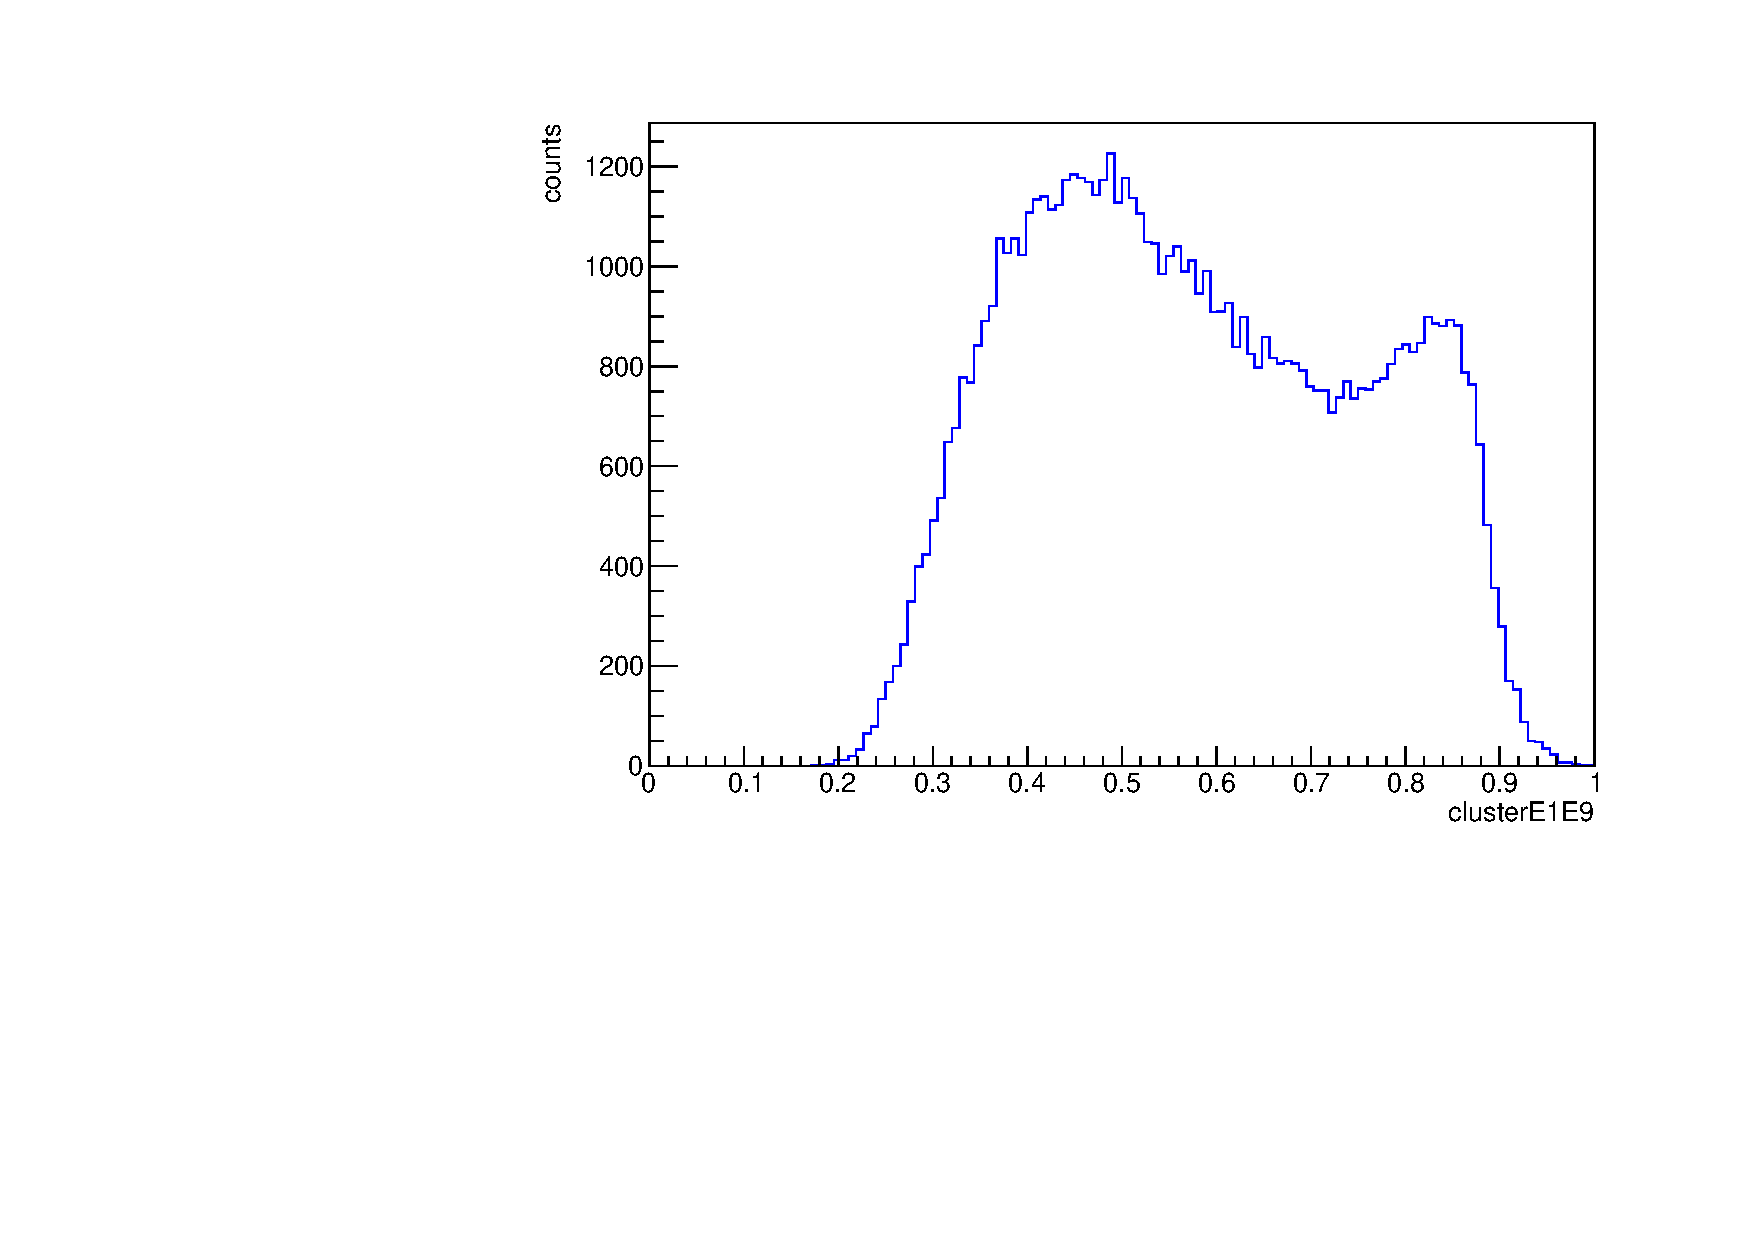
\includegraphics[width=0.49\textwidth]{nbar_cocktail/images/clusterE1E9_isr_qqbar.pdf}
    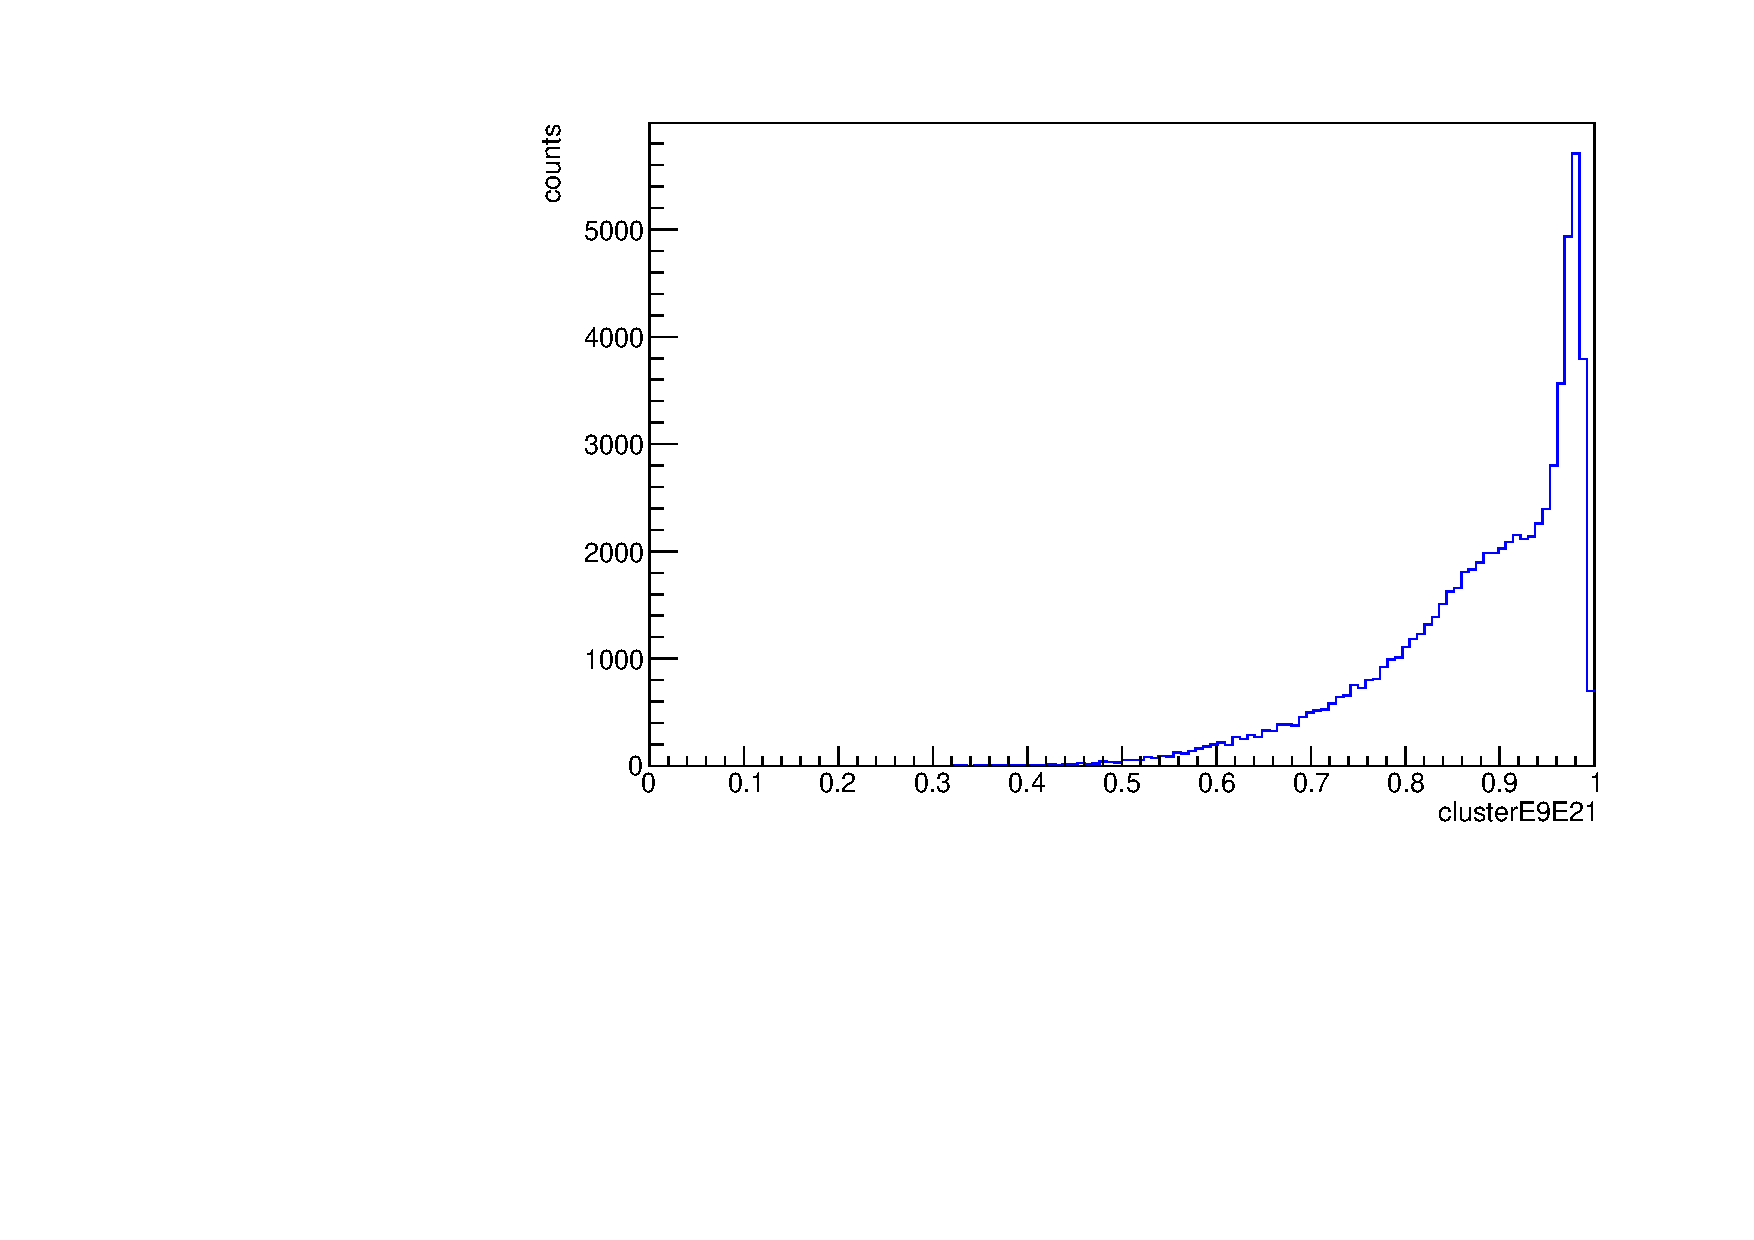
\includegraphics[width=0.49\textwidth]{nbar_cocktail/images/clusterE9E21_isr_qqbar.pdf}
    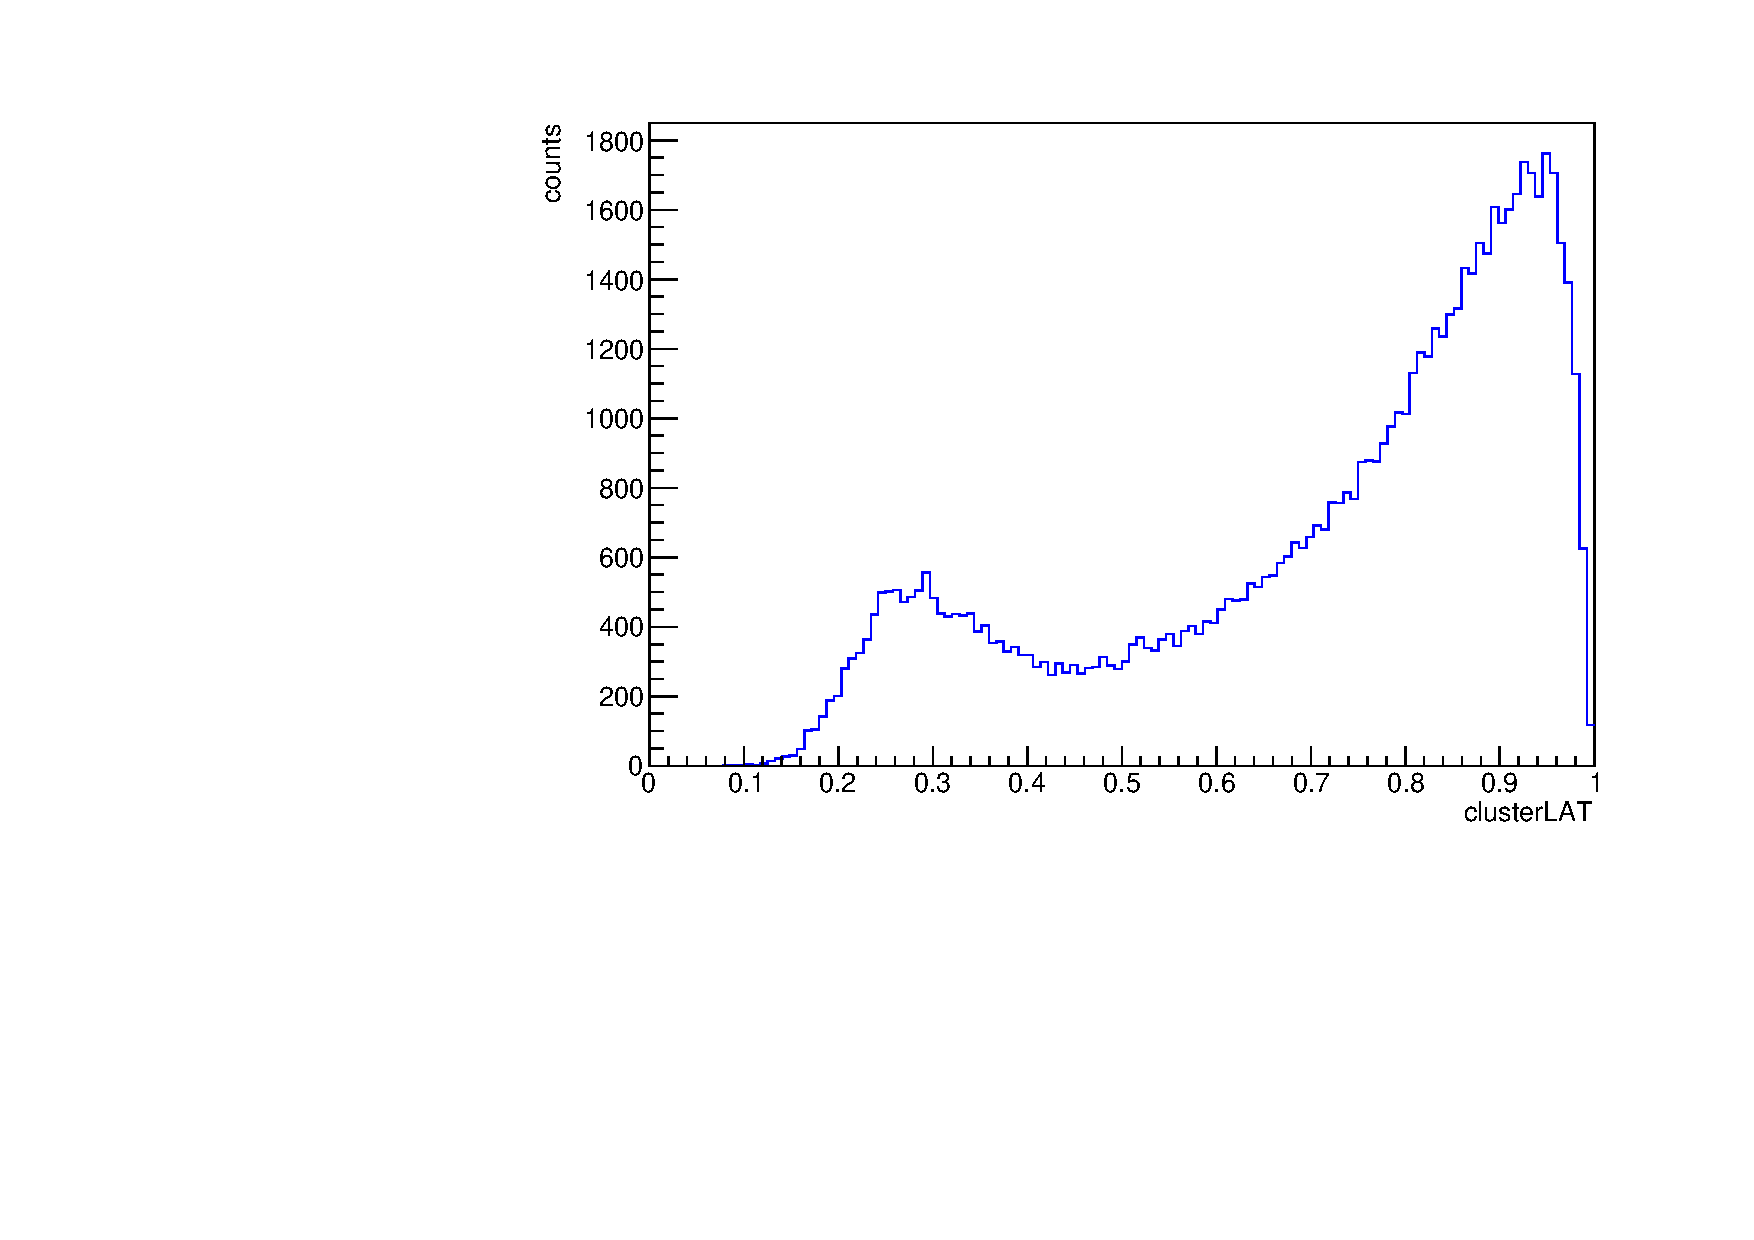
\includegraphics[width=0.49\textwidth]{nbar_cocktail/images/clusterLAT_isr_qqbar.pdf}
    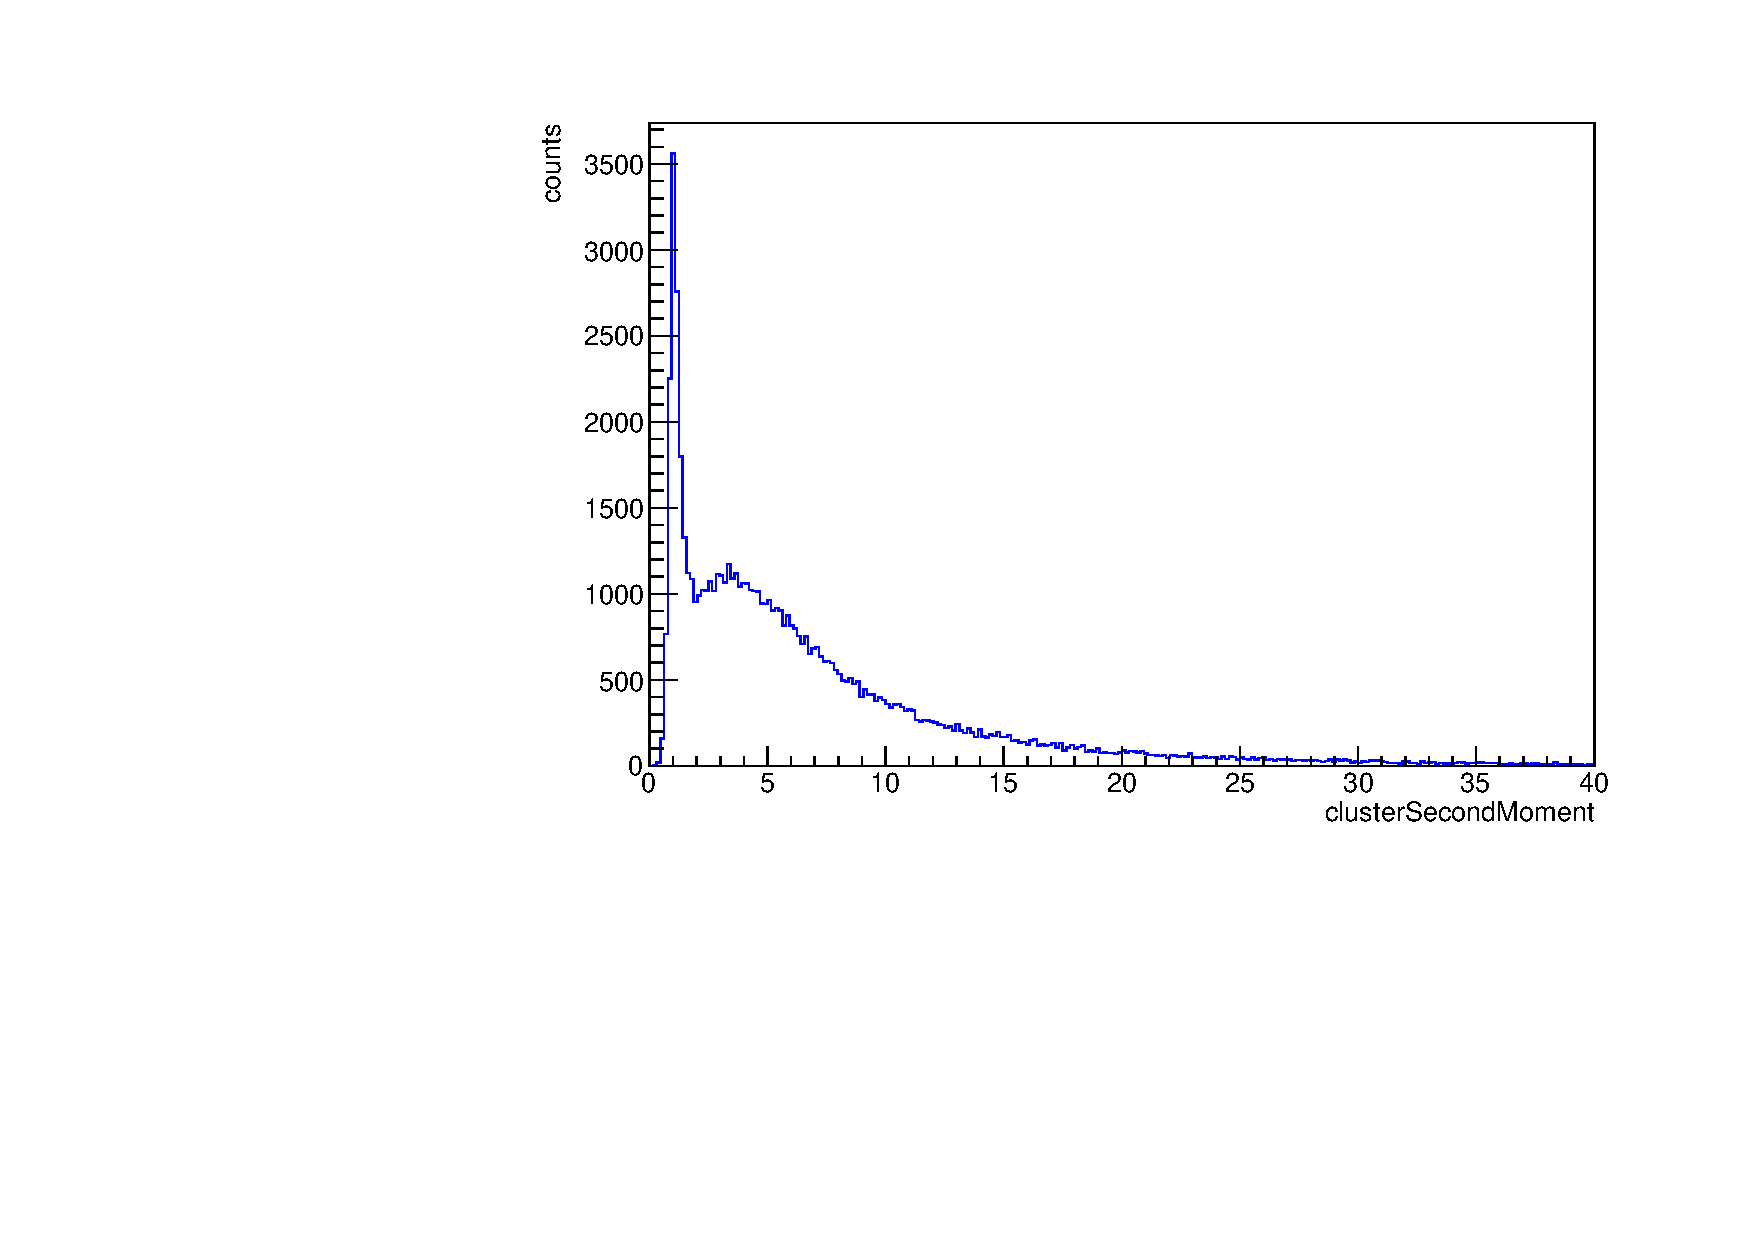
\includegraphics[width=0.49\textwidth]{nbar_cocktail/images/clusterSecondMoment_isr_qqbar.pdf}
    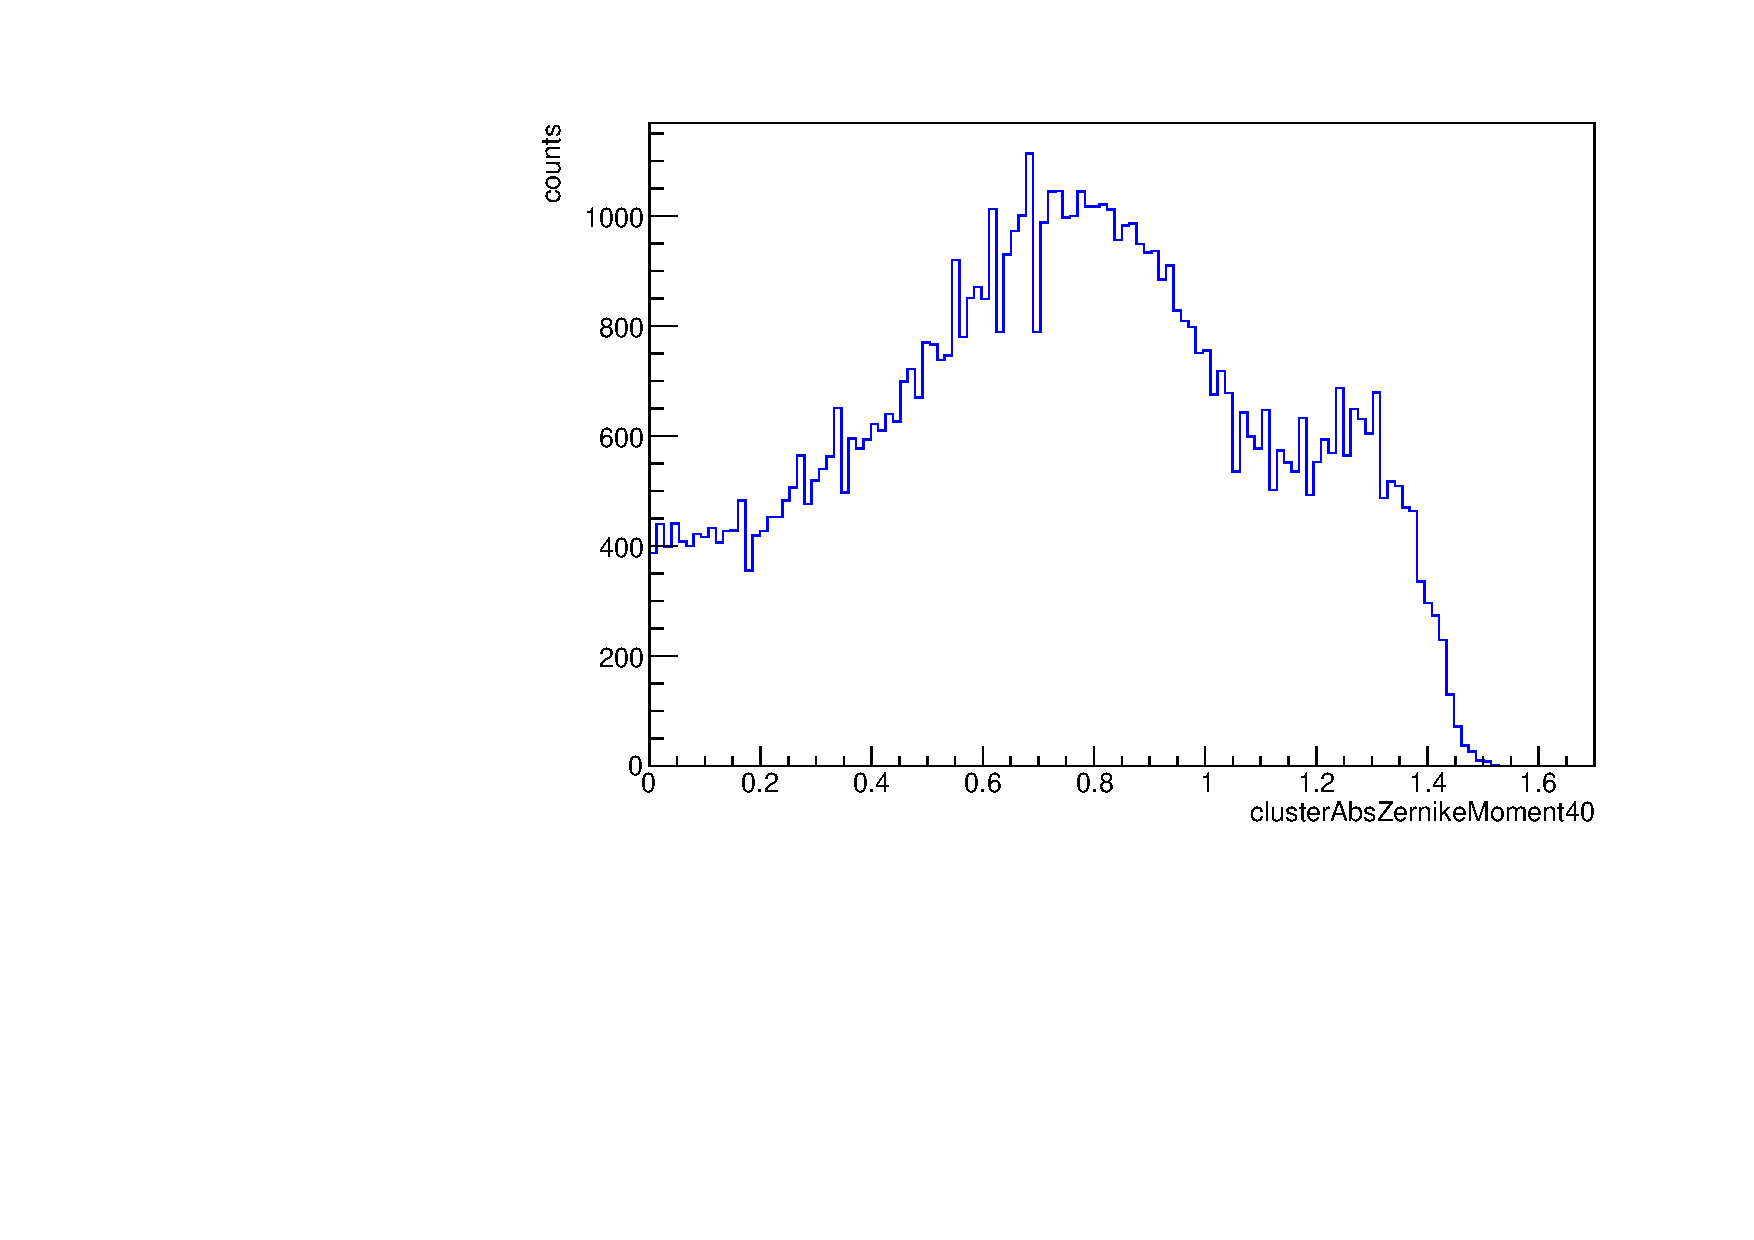
\includegraphics[width=0.49\textwidth]{nbar_cocktail/images/clusterAbsZernikeMoment40_isr_qqbar.pdf}
    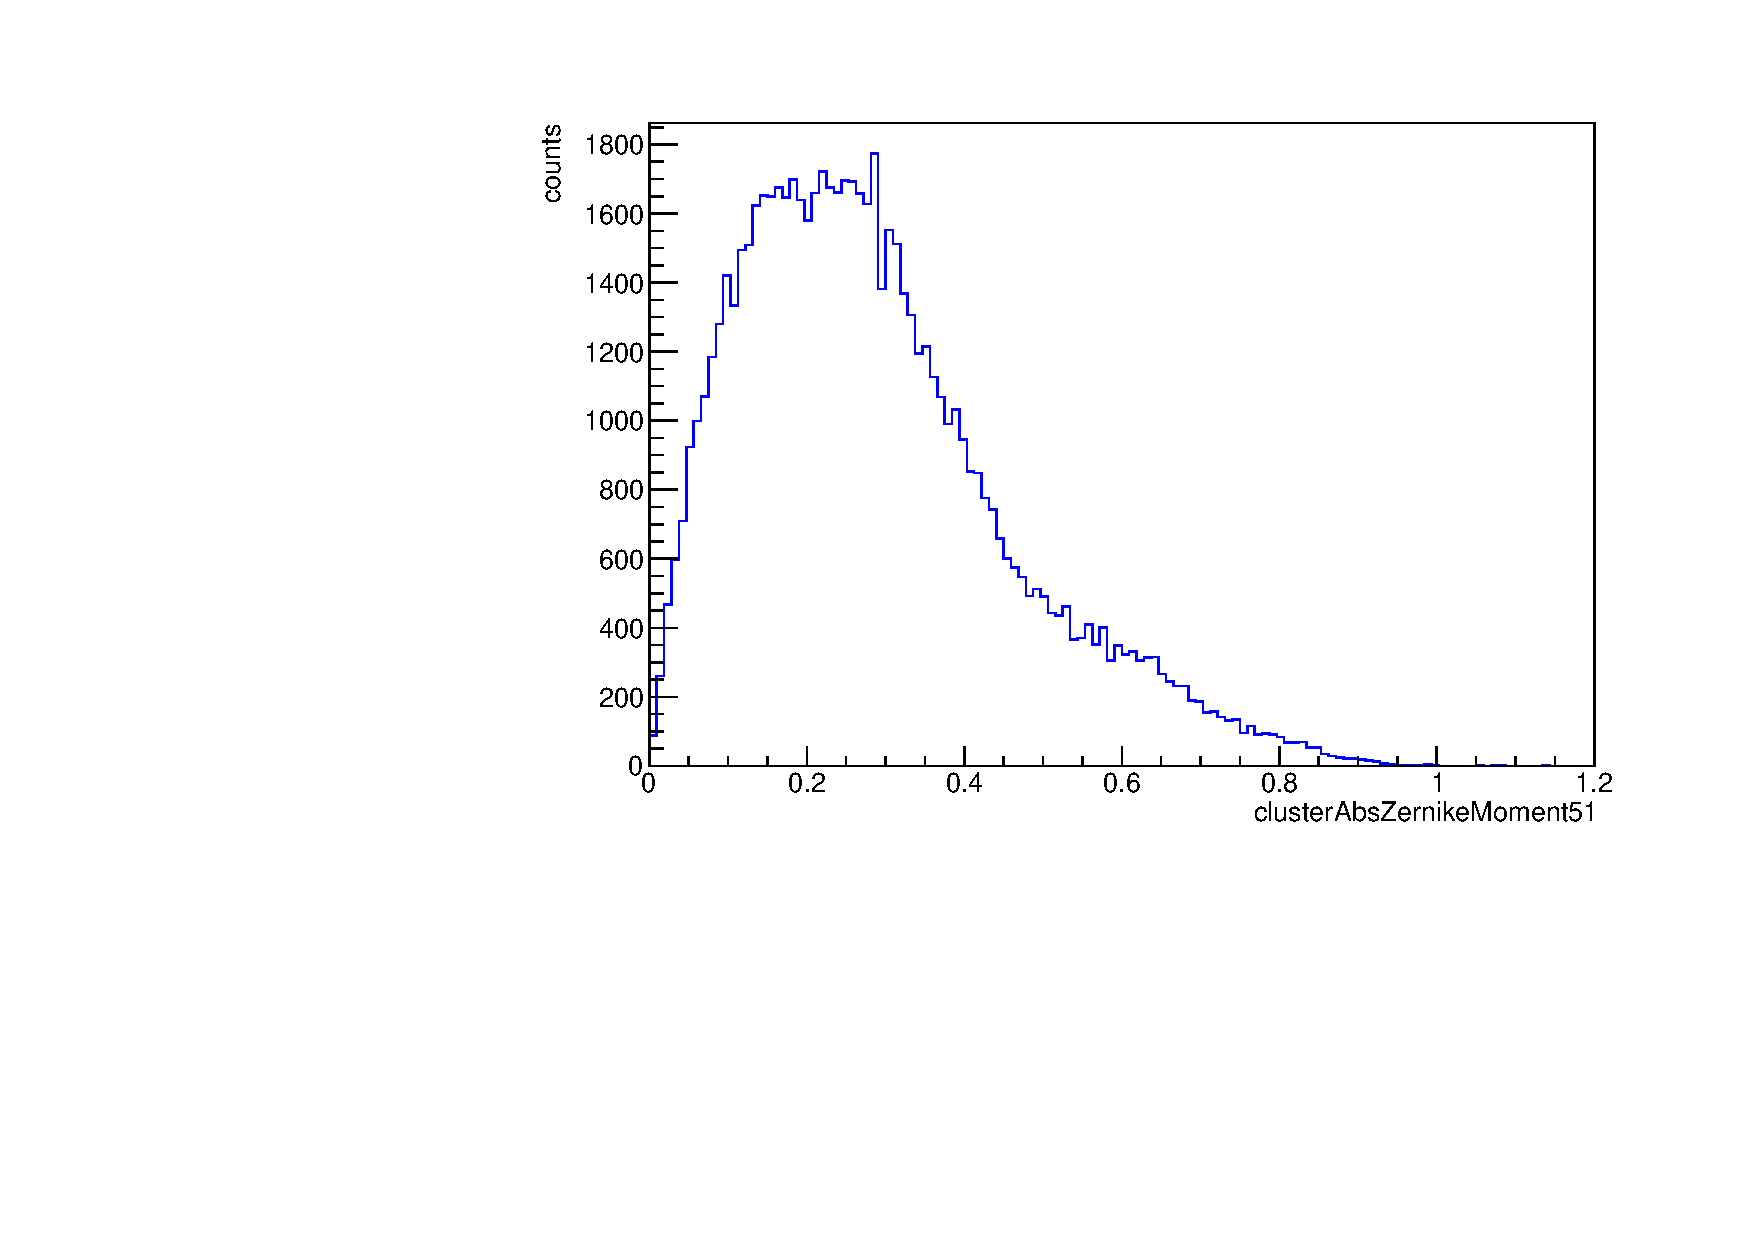
\includegraphics[width=0.49\textwidth]{nbar_cocktail/images/clusterAbsZernikeMoment51_isr_qqbar.pdf}
    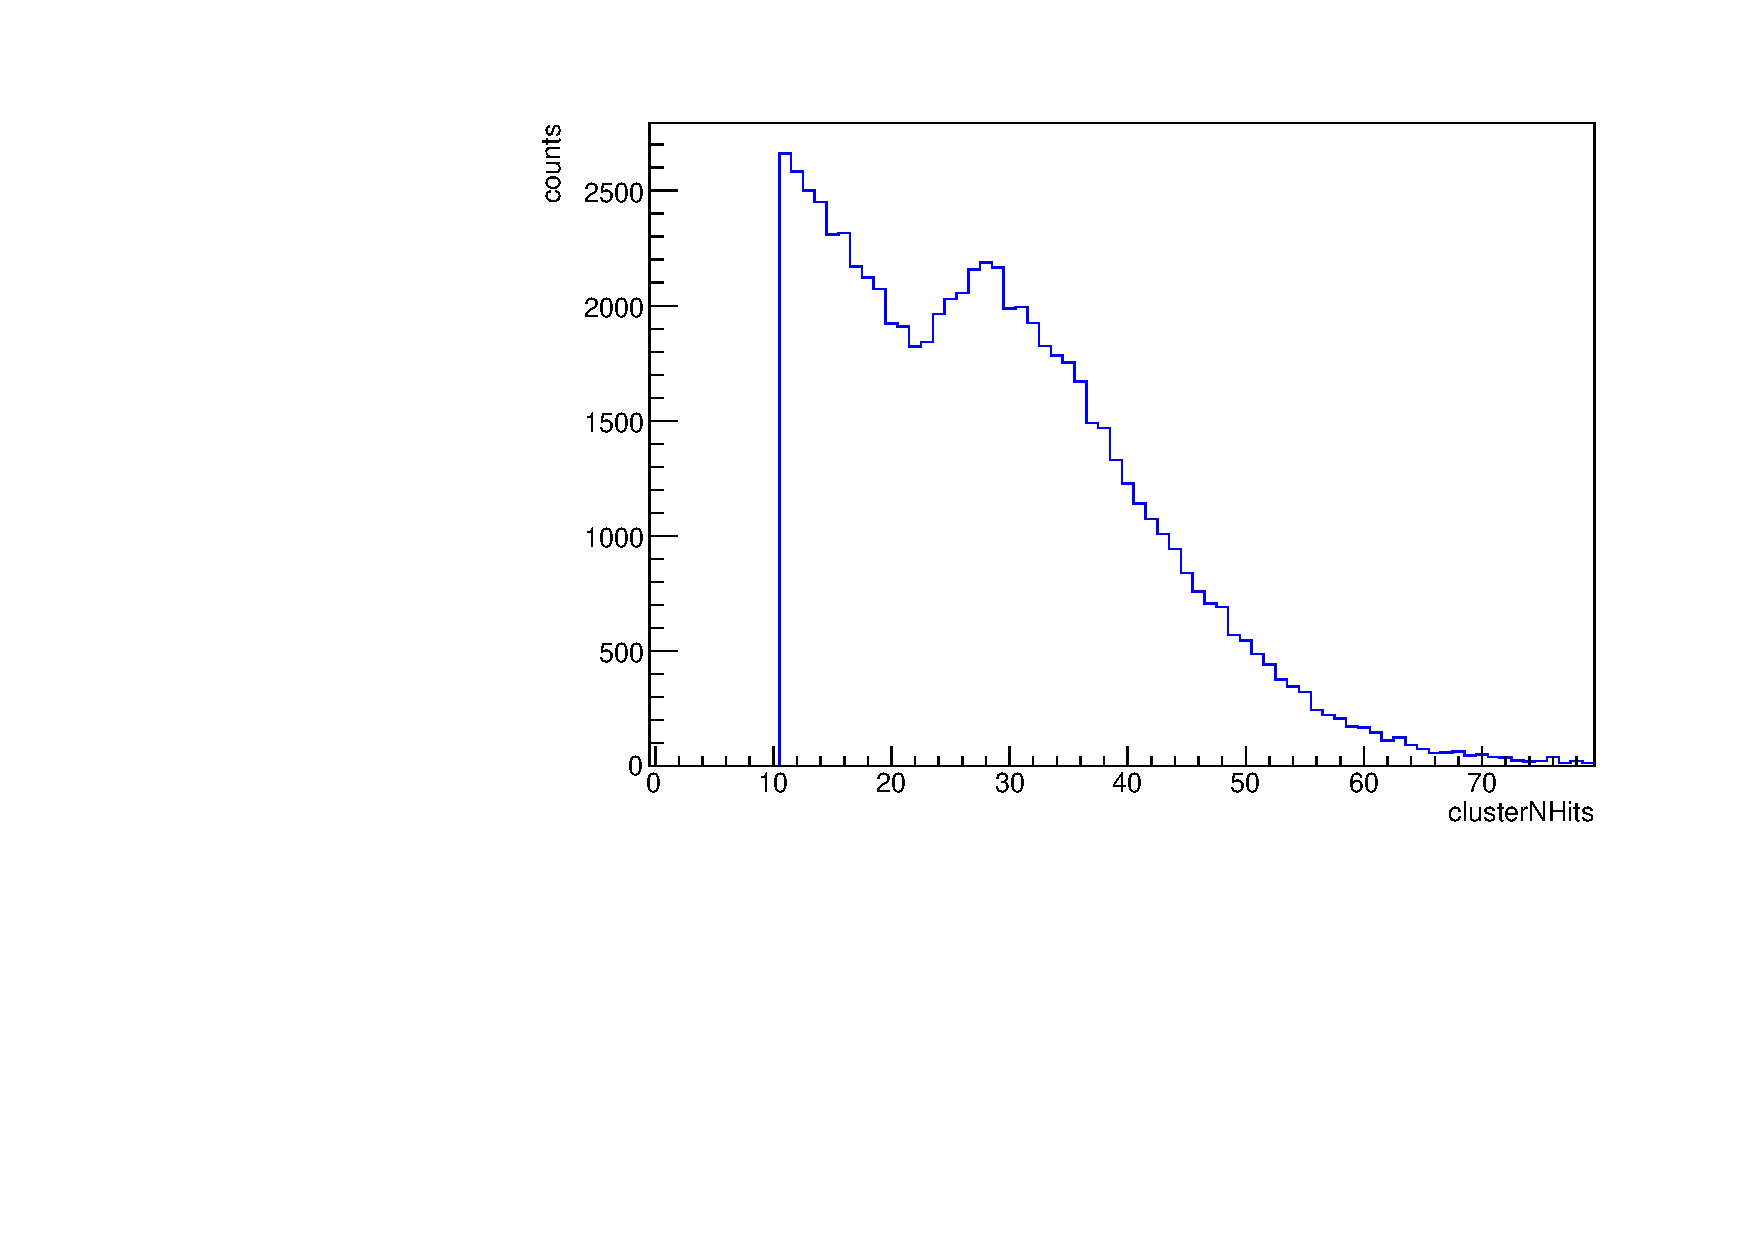
\includegraphics[width=0.49\textwidth]{nbar_cocktail/images/clusterNHits_isr_qqbar.pdf}
     \caption{Reconstructed cluster variables distribution for $\bar{n}$ candidates in the for the recoil mass region [0, 2] GeV, in ISR case. q$\bar{q}$ cocktail }
     \label{fig:clus_vars_isr_qqbar}
\end{figure}
$\\$
Since substantial background appears to the right of the signal region -suggesting that particles are missing from the recoil reconstruction- the sideband regions are redefined, for the ISR case, as follows:
\begin{itemize}
\item Signal region: [0.8, 1.4] GeV;
\item Sidebands regions: [0.2, 0.8] U [1.4, 2.0]  GeV;
\item $k = \frac{1.4 - 0.8}{(0.8 - 0.2) + (2.0 - 1.4)} = \frac{1}{2}$.
\end{itemize}

The signal region and sidebands region, in the recoil mass distribution  are shown in Fig.\ref{fig:recMass_sidebands_isr}.
\begin{figure}[H]
    \centering
    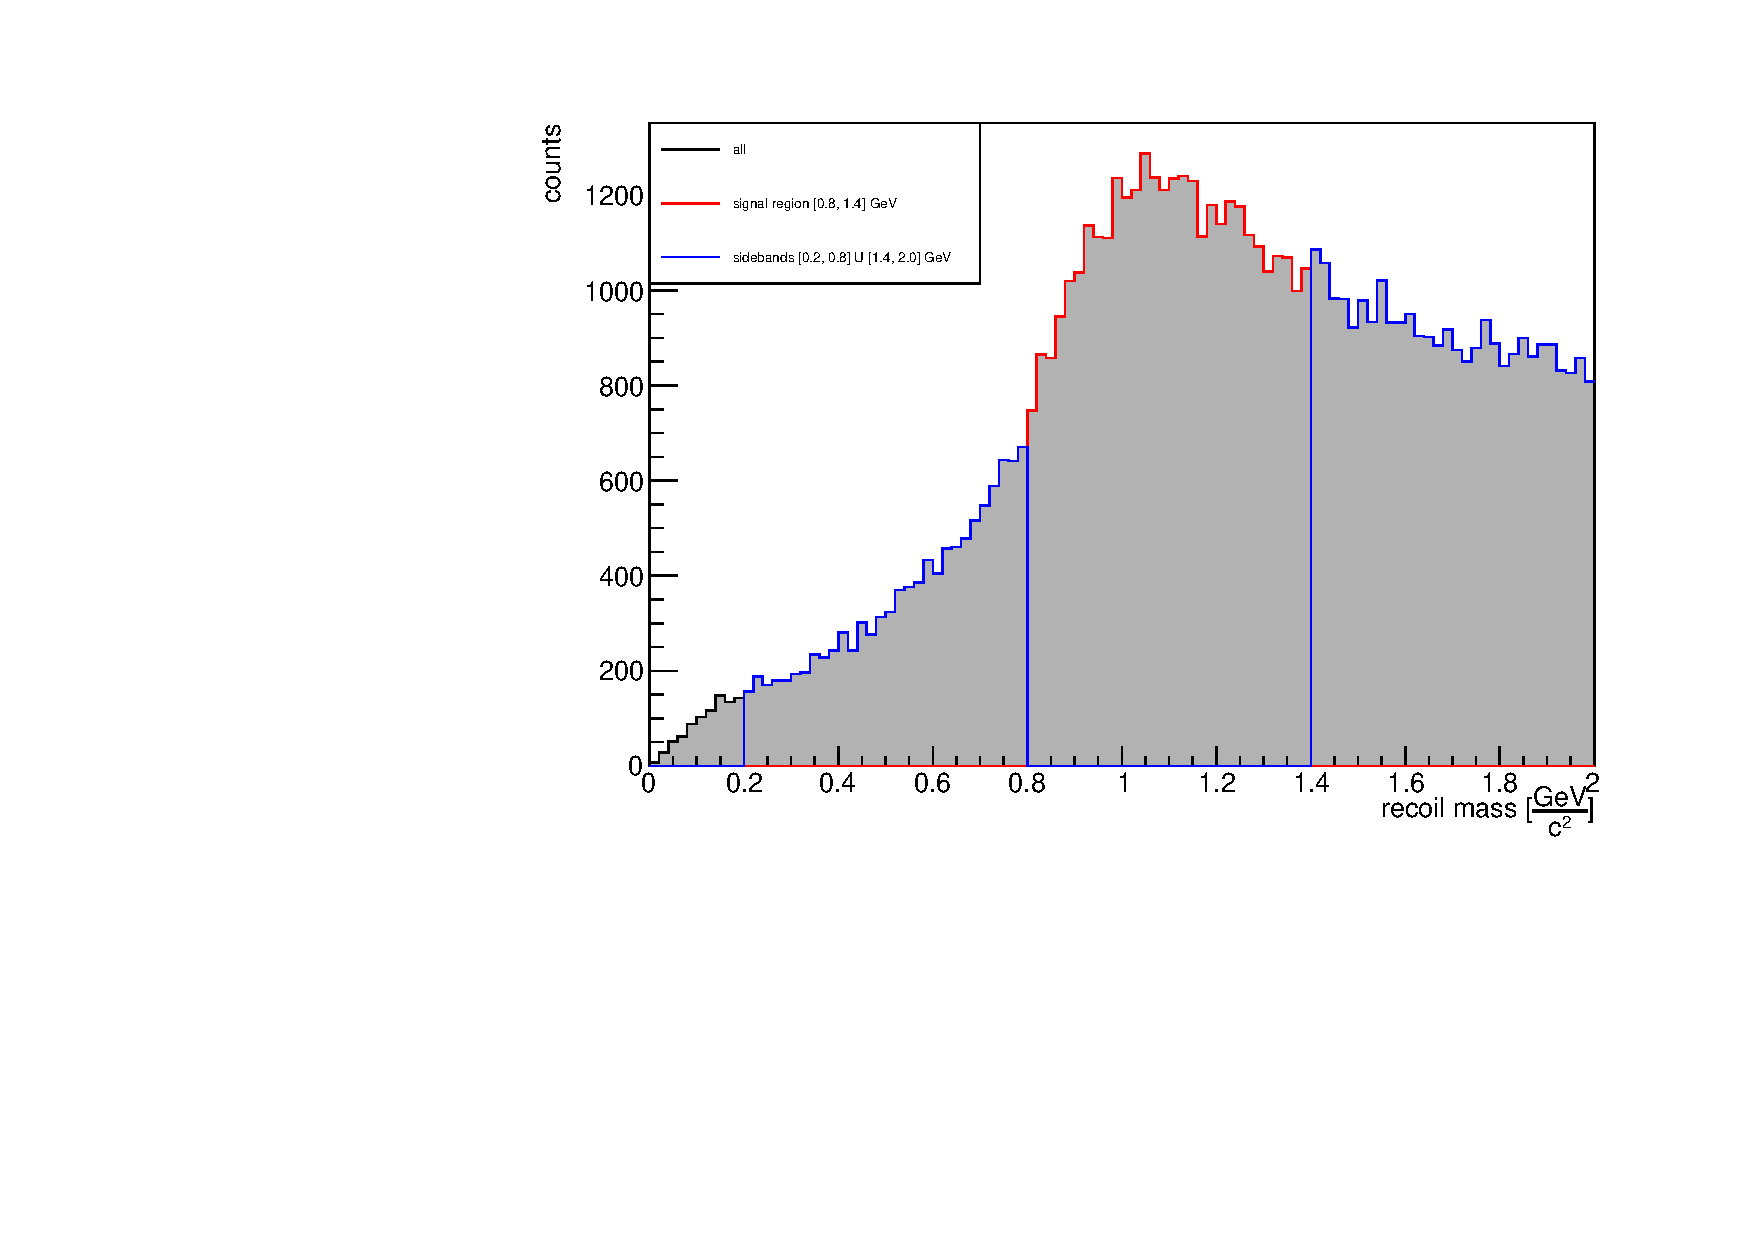
\includegraphics[width=0.6\textwidth]{nbar_cocktail/images/recoil_mass_sidebands_isr}
    \caption{Recoil mass distribution (black), with the signal region (red) and the sidebands regions (blue), in the $q\bar{q}$ Monte Carlo cocktail. ISR case.}
    \label{fig:recMass_sidebands_isr}
\end{figure}

The obtained cluster variables contribution is shown in Fig.\ref{fig:clus_vars_sidebands_pre_isr}.
 \begin{figure}[h]
    \centering
    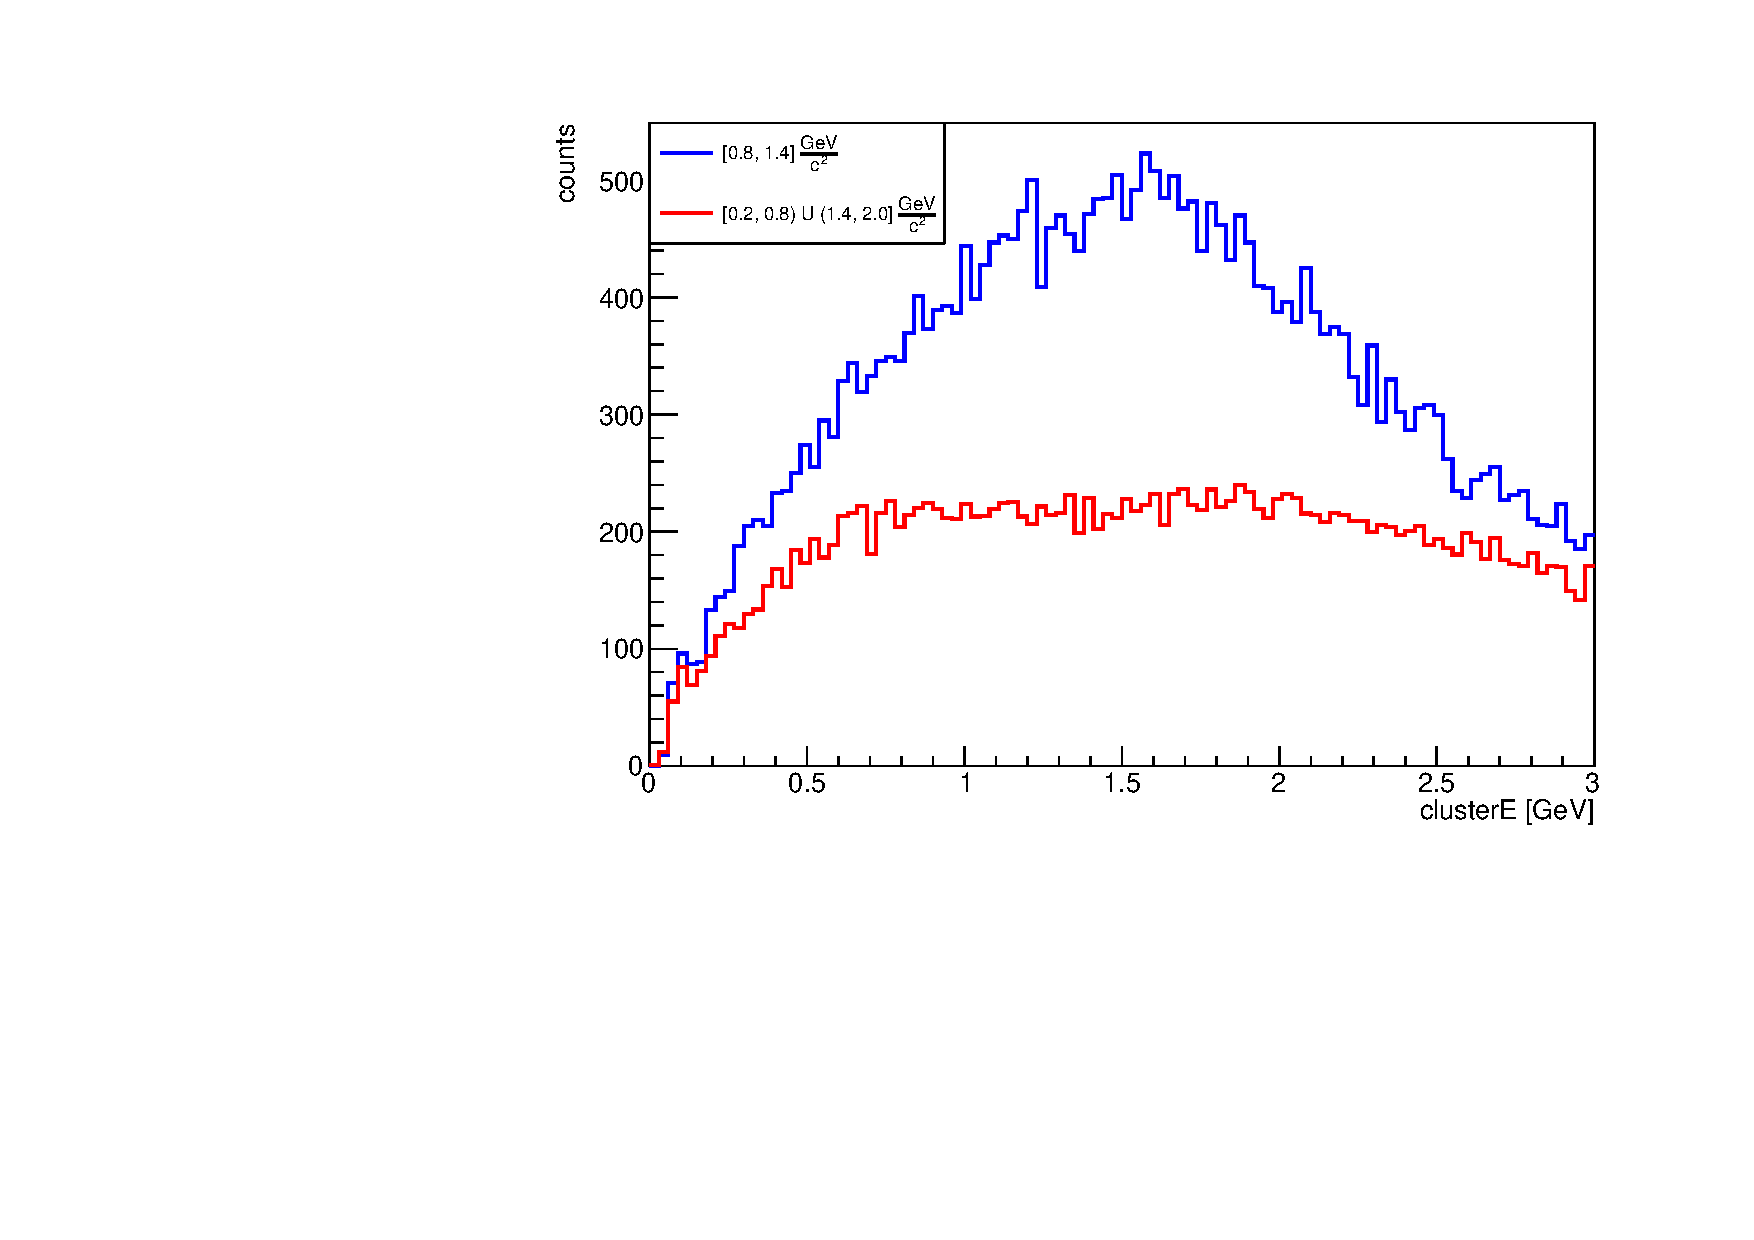
\includegraphics[width=0.49\textwidth]{nbar_cocktail/images/sidebands_clusterE_isr.pdf}
    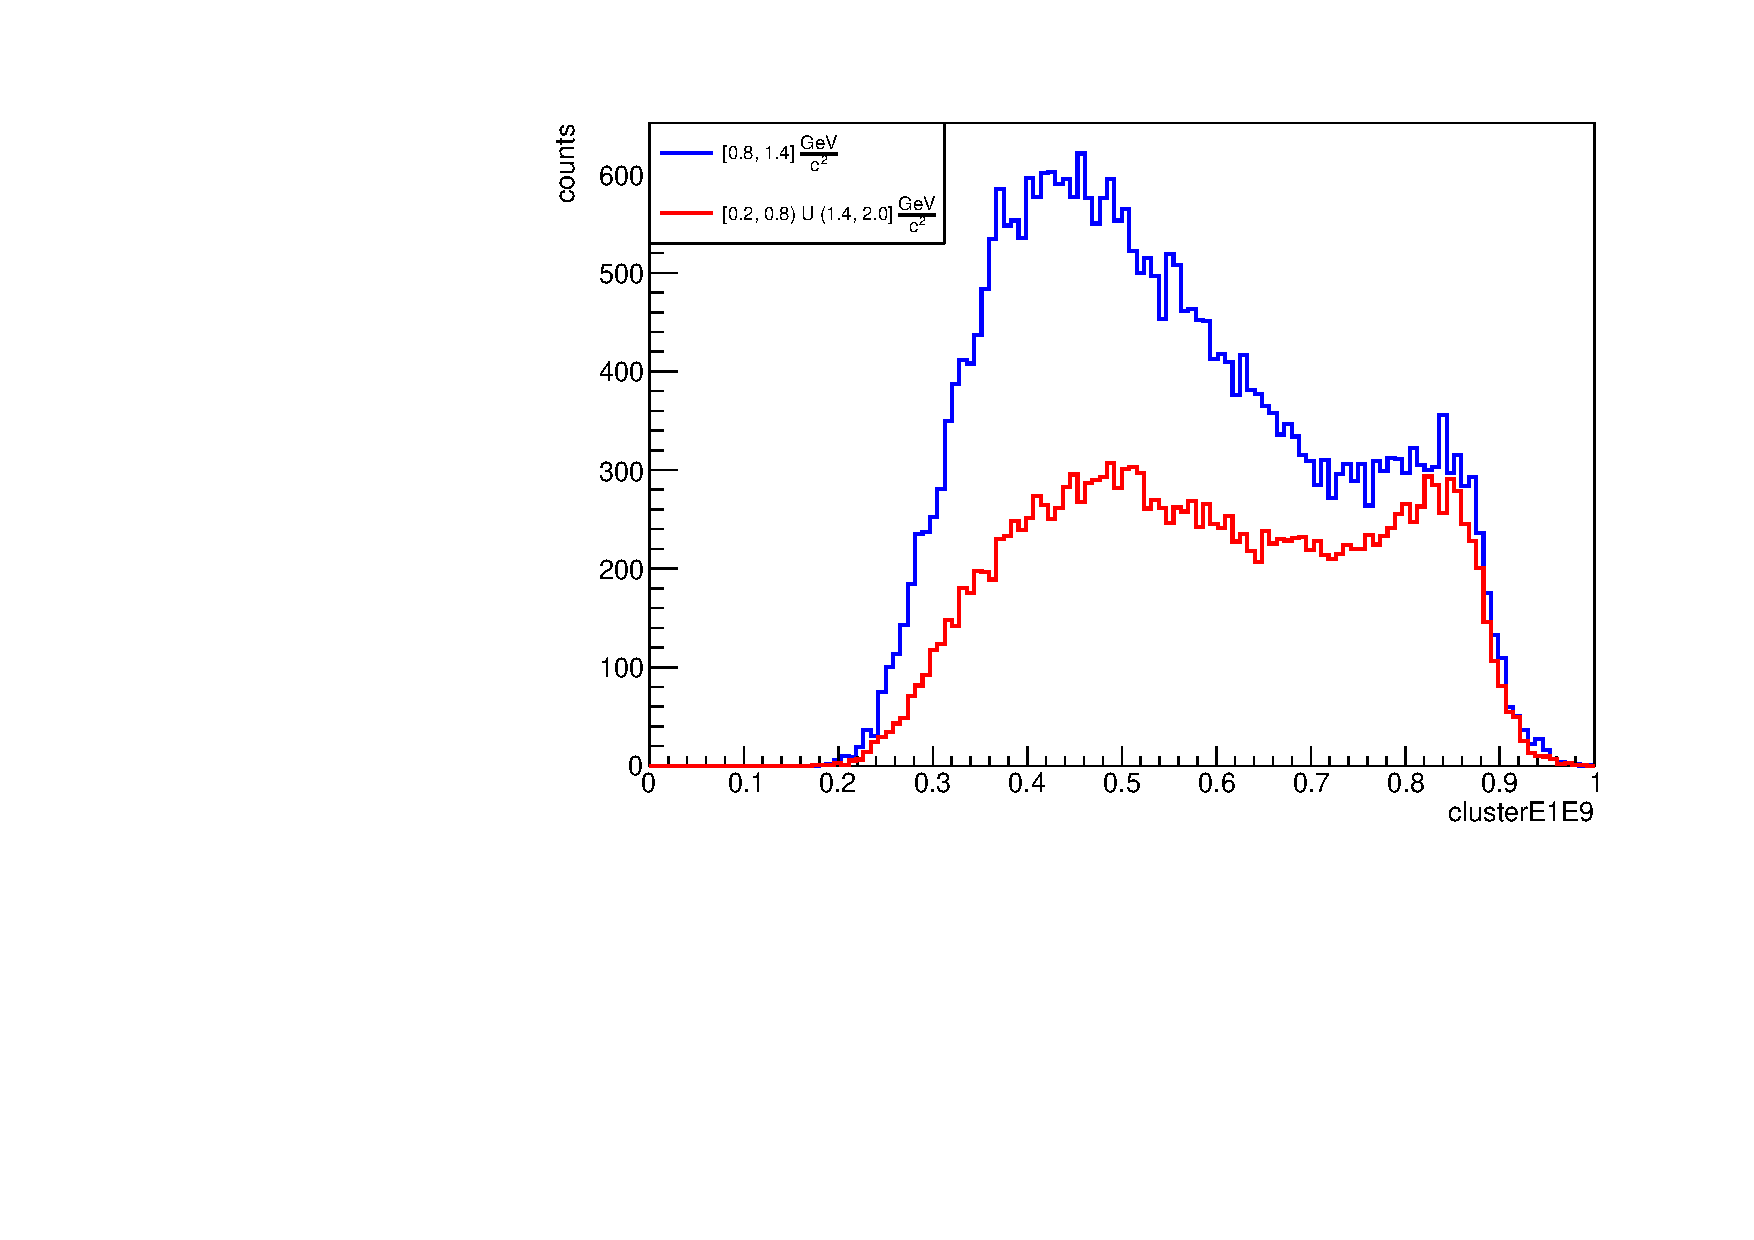
\includegraphics[width=0.49\textwidth]{nbar_cocktail/images/sidebands_clusterE1E9_isr.pdf}
    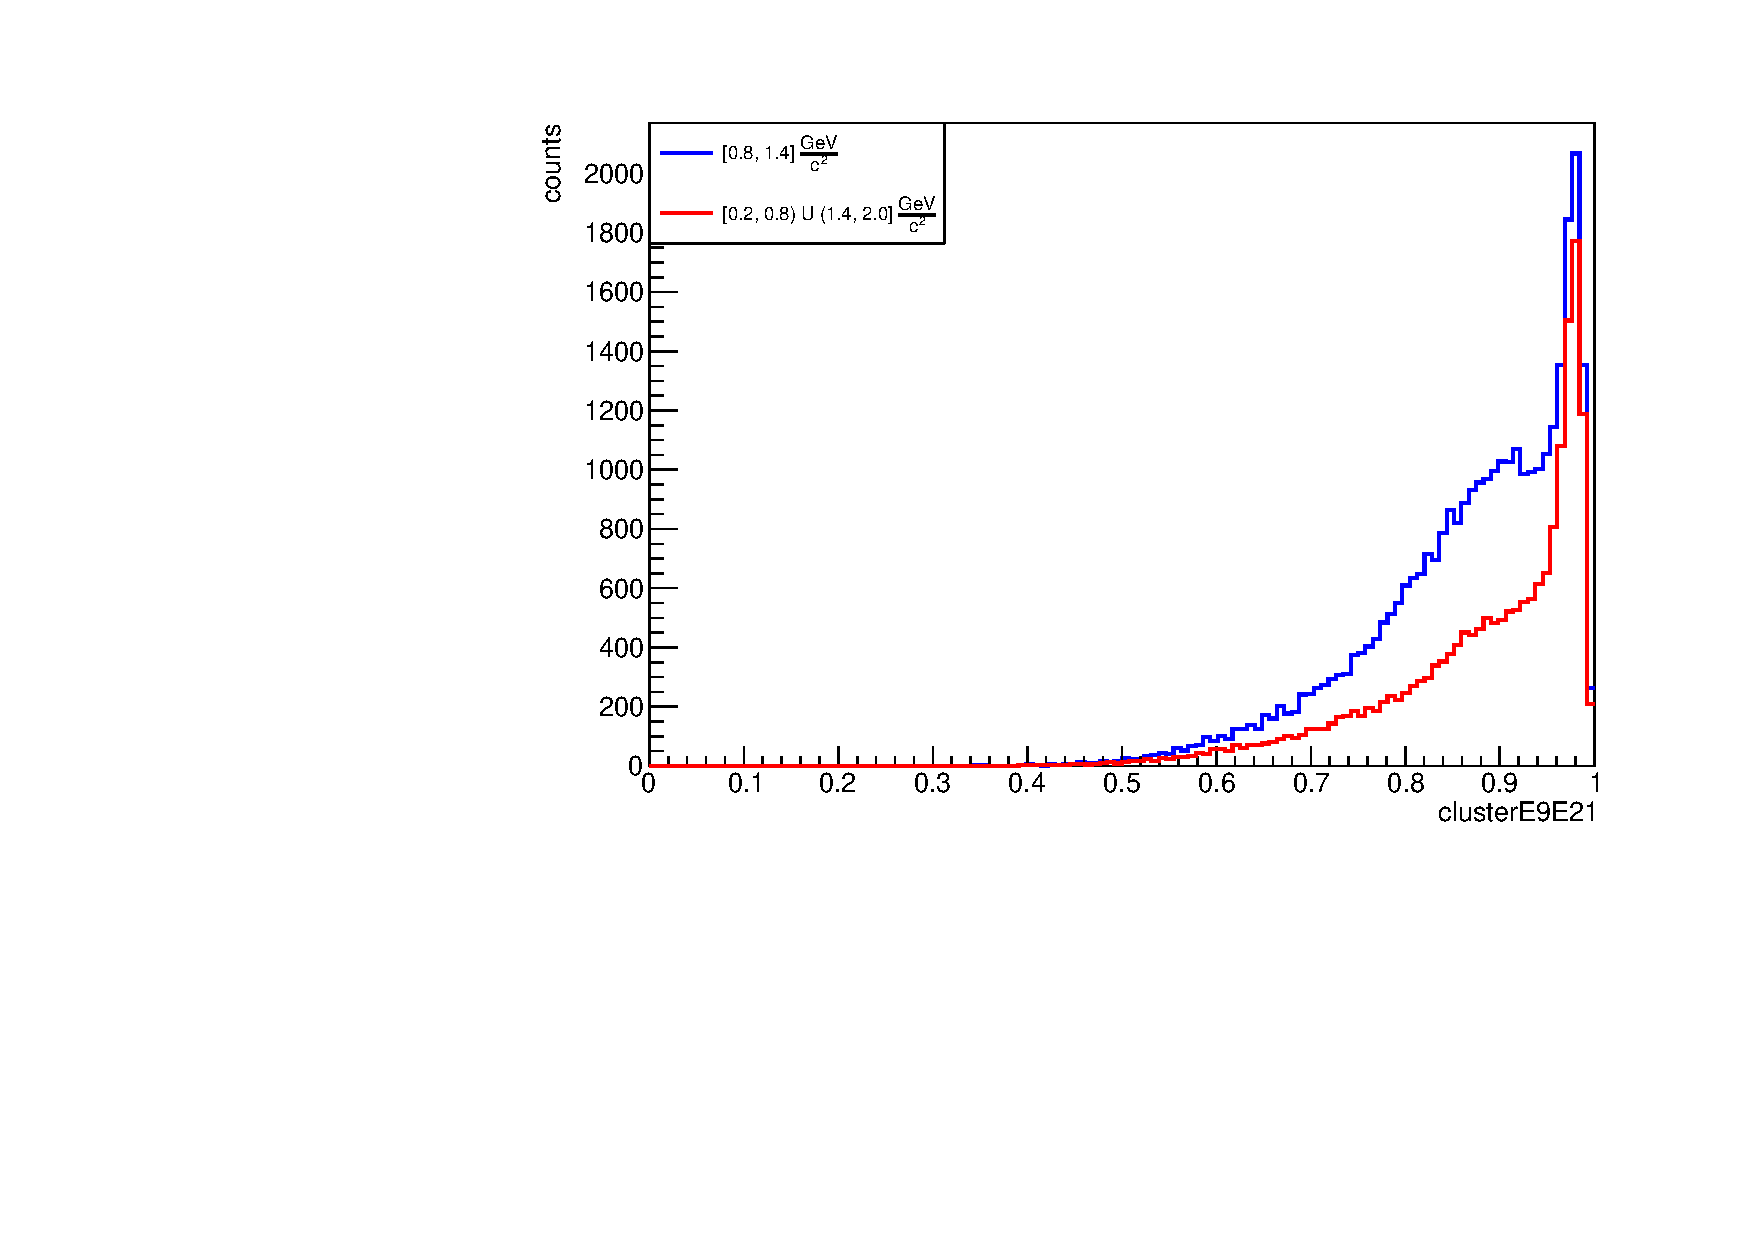
\includegraphics[width=0.49\textwidth]{nbar_cocktail/images/sidebands_clusterE9E21_isr.pdf}
    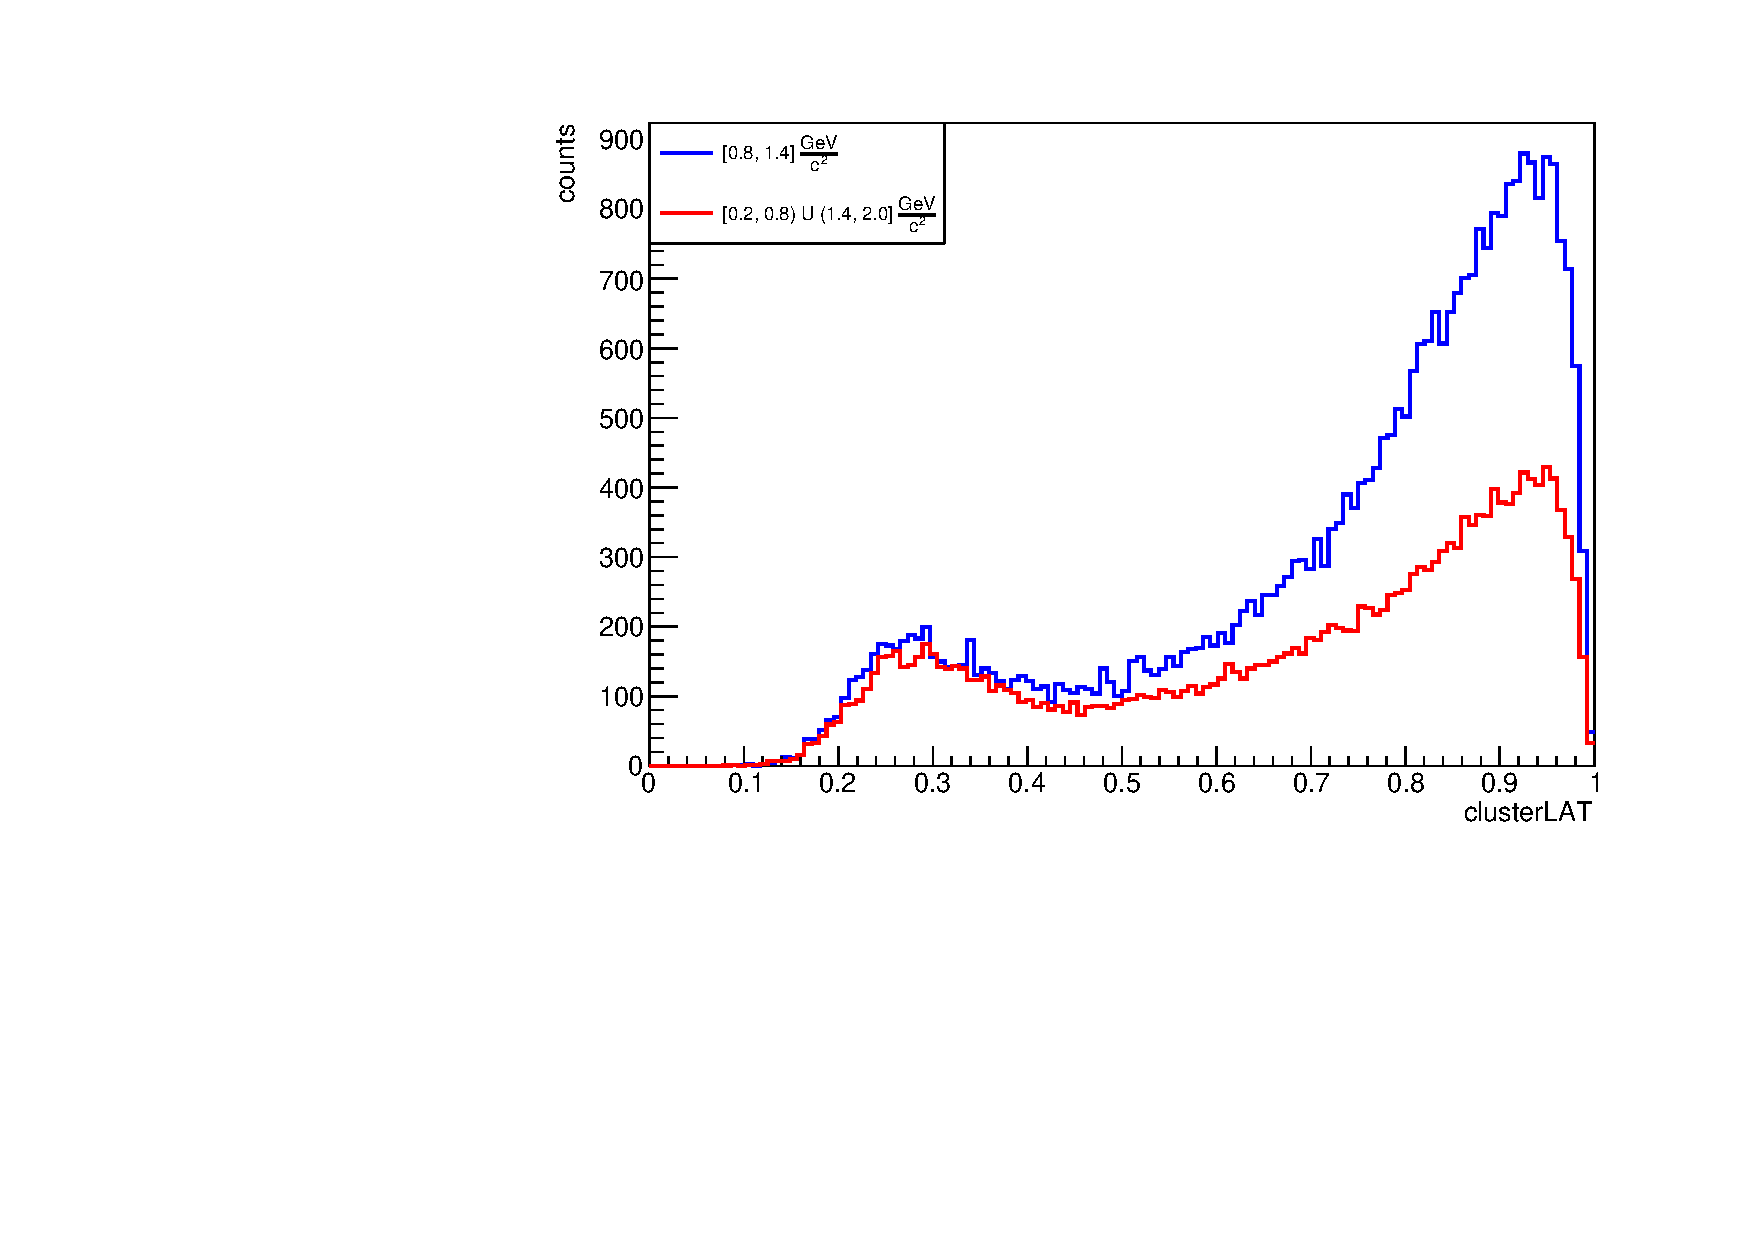
\includegraphics[width=0.49\textwidth]{nbar_cocktail/images/sidebands_clusterLAT_isr.pdf}
    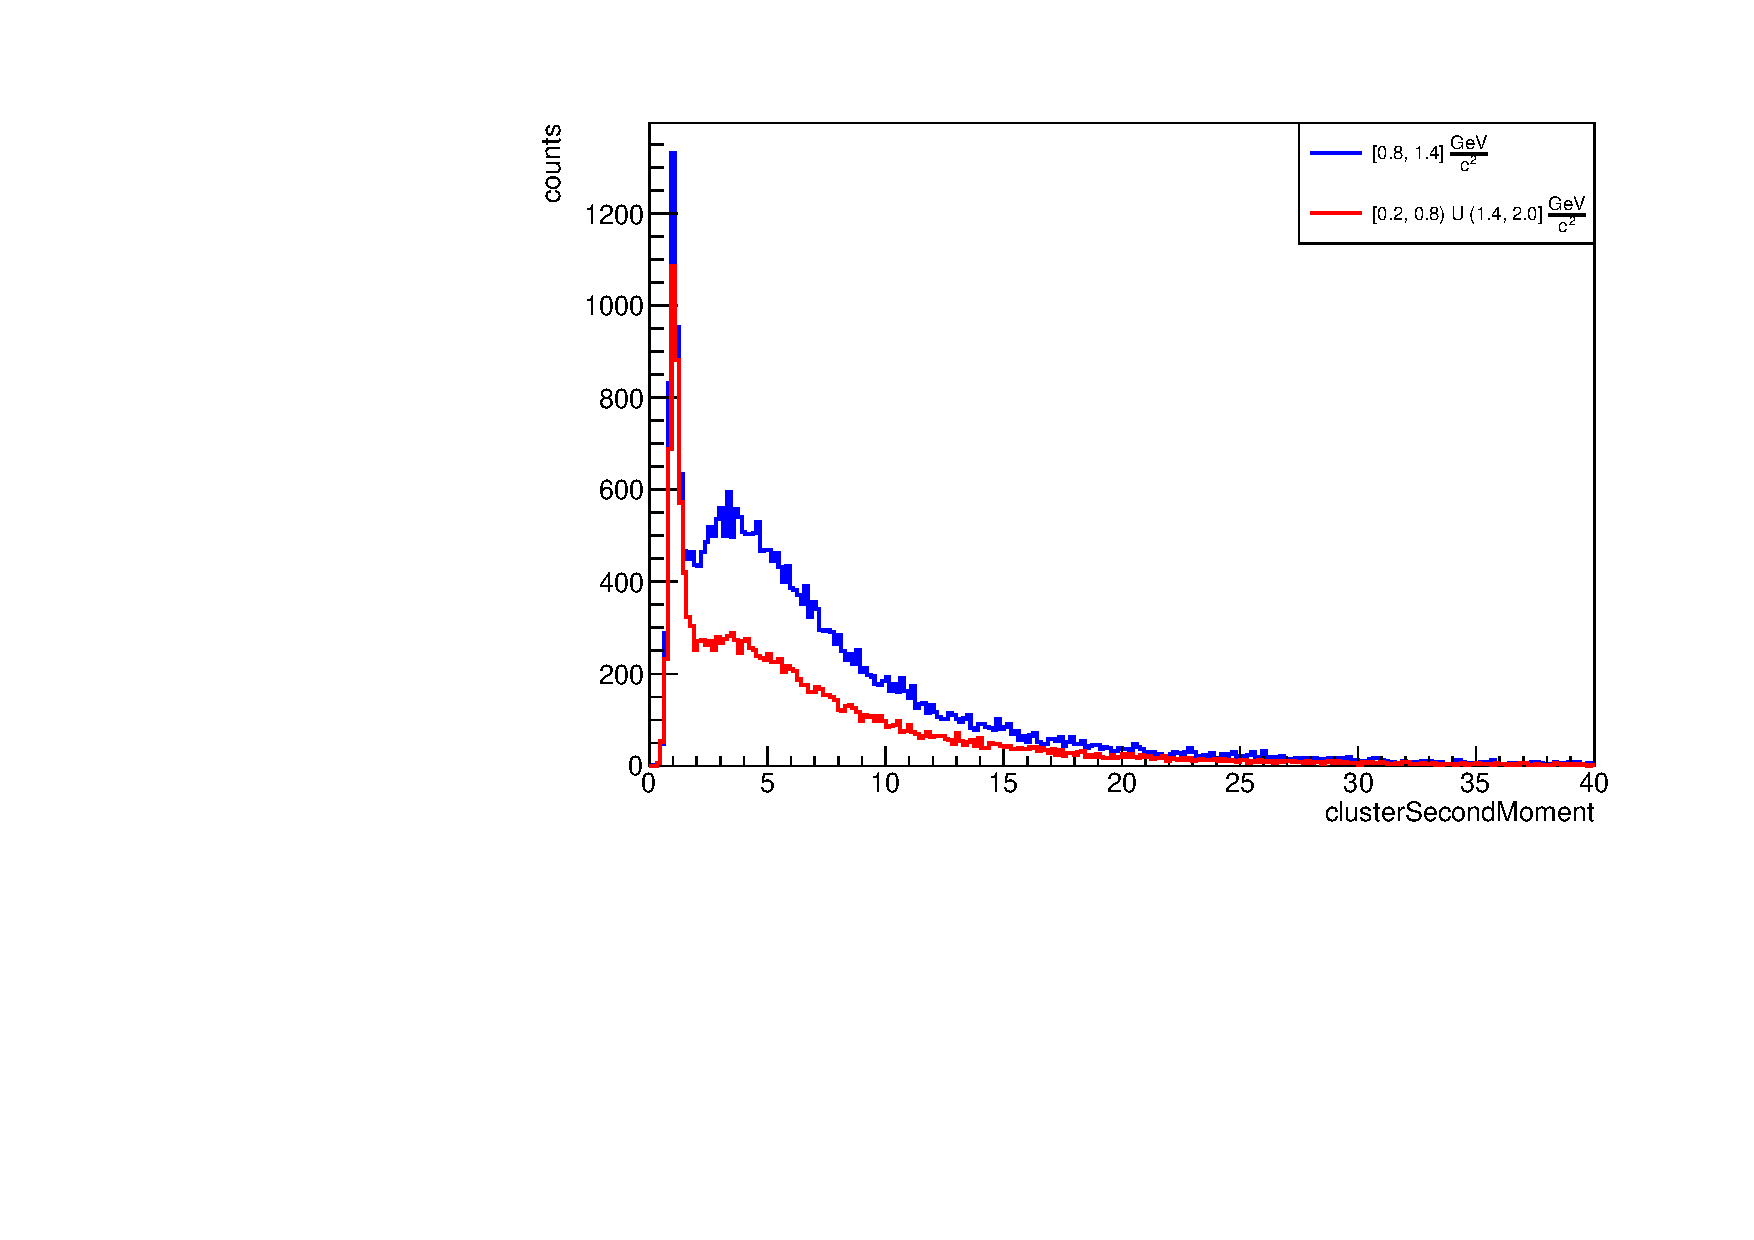
\includegraphics[width=0.49\textwidth]{nbar_cocktail/images/sidebands_clusterSecondMoment_isr.pdf}
    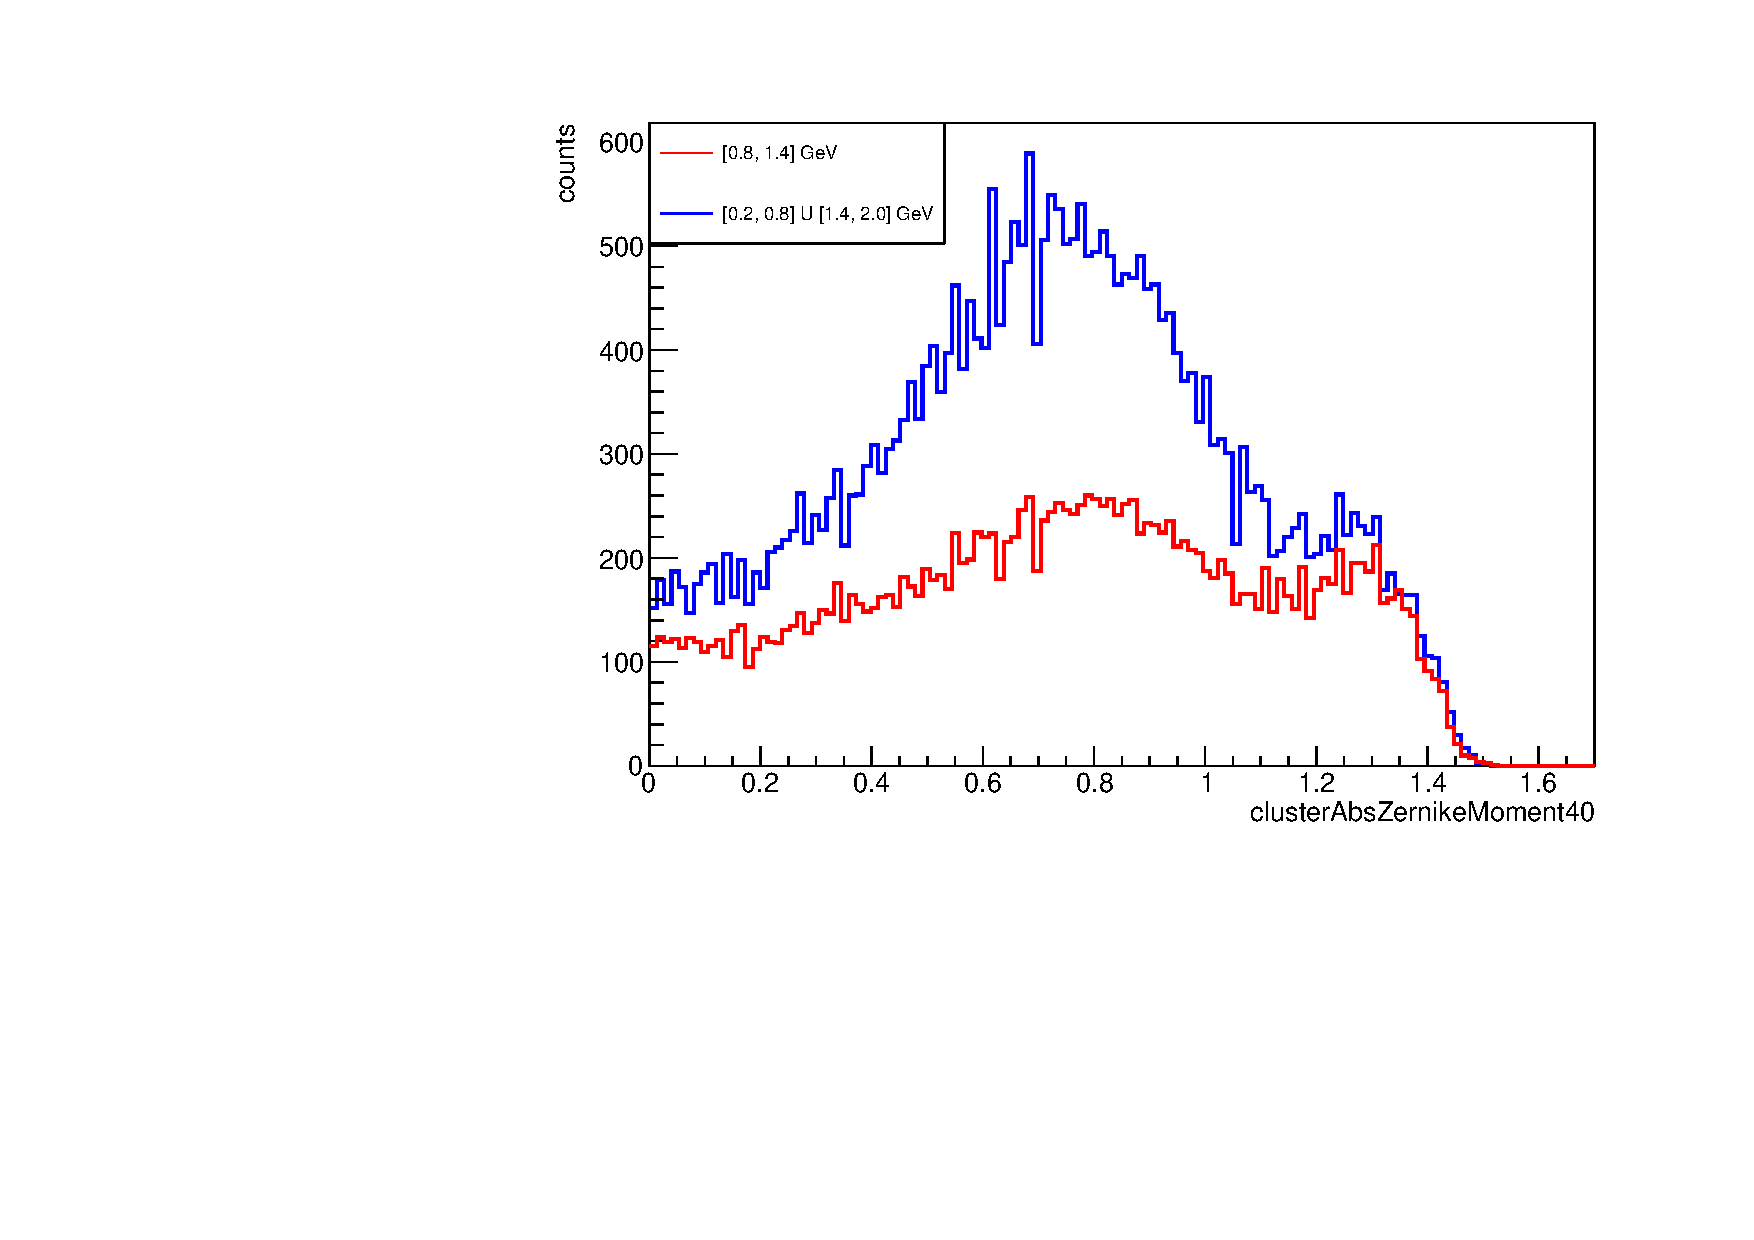
\includegraphics[width=0.49\textwidth]{nbar_cocktail/images/sidebands_clusterAbsZernikeMoment40_isr.pdf}
    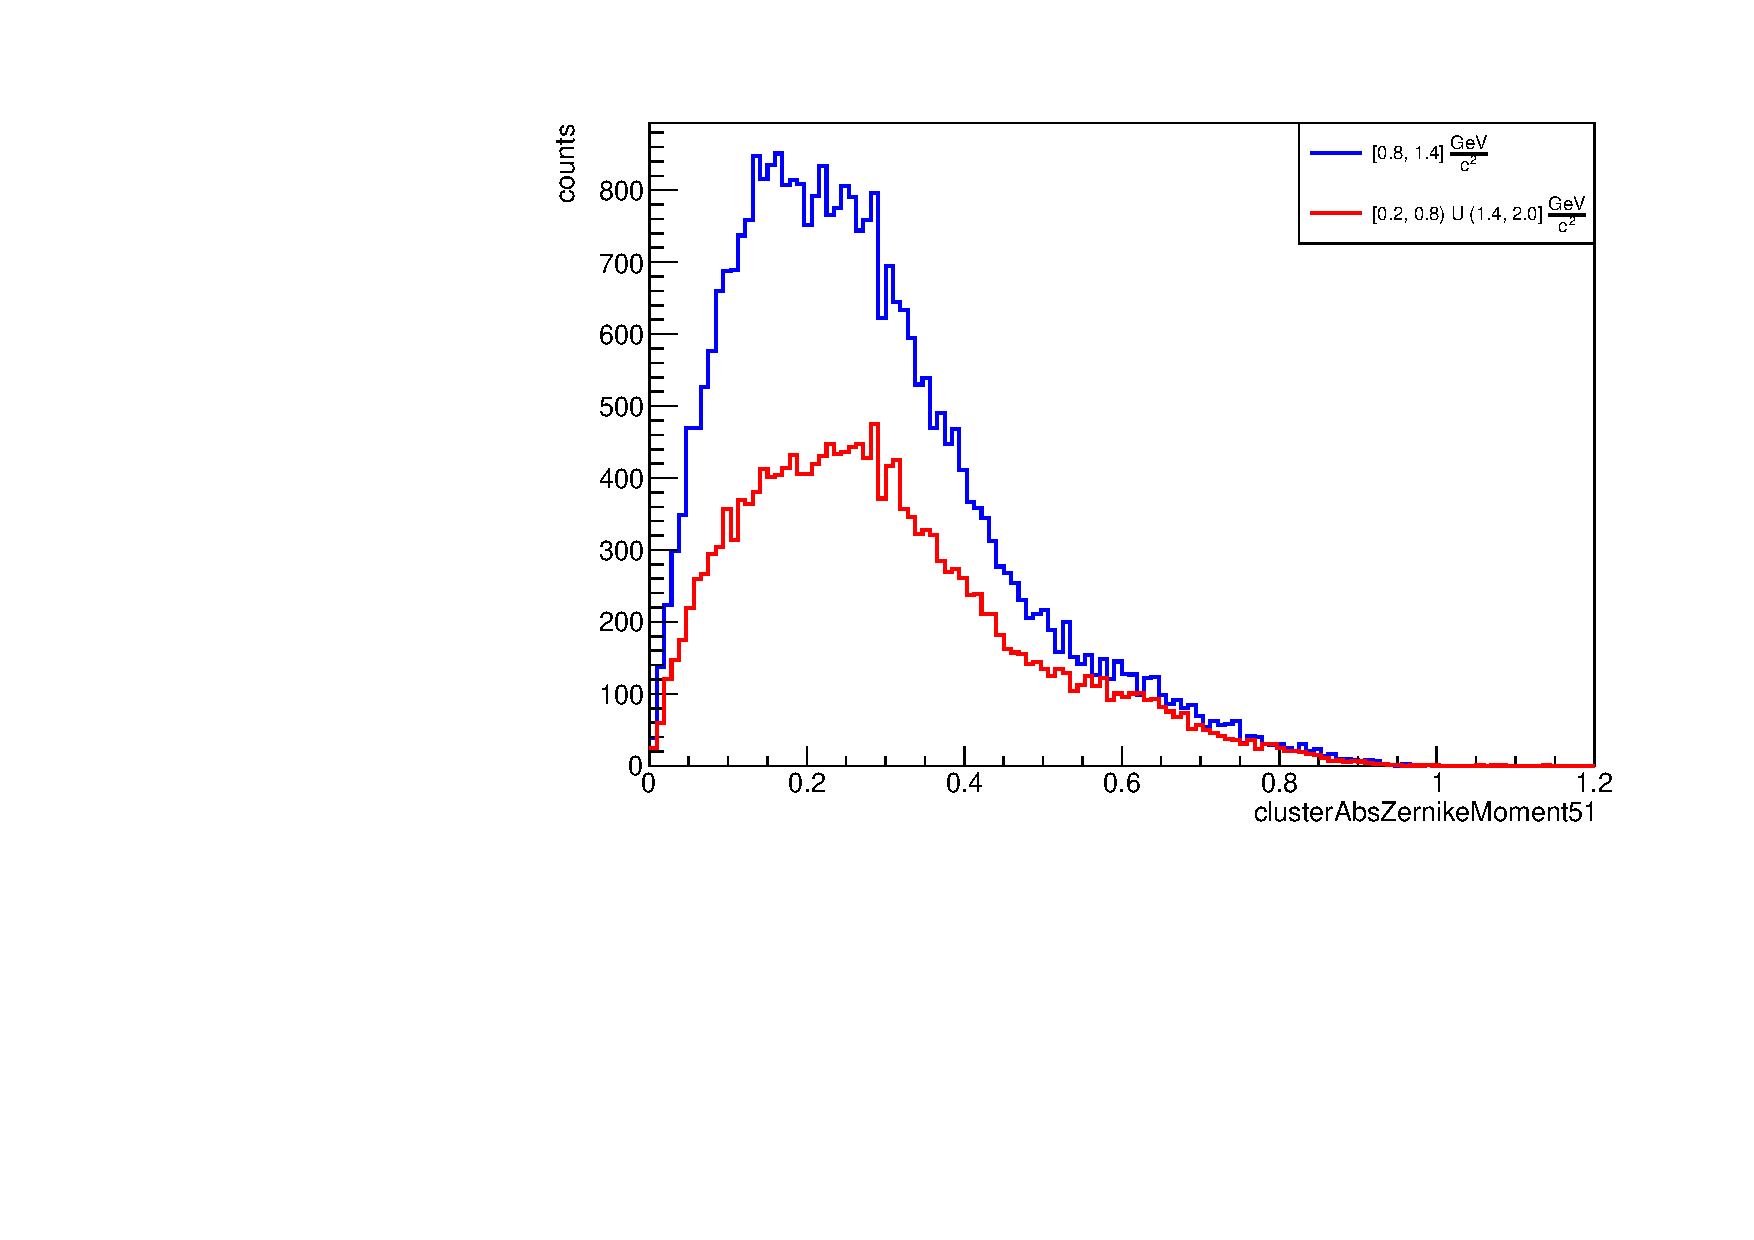
\includegraphics[width=0.49\textwidth]{nbar_cocktail/images/sidebands_clusterAbsZernikeMoment51_isr.pdf}
    \includegraphics[width=0.49\textwidth]{nbar_cocktail/images/sidebands_clusterNHits_isr.pdf}
     \caption{Comparison of reconstructed cluster variables for $\bar{n}$ candidates in the signal region [0.8, 1.2] GeV (blue) with $\bar{n}$ candidates in the sidebands region [0.3, 0.7] U [1.3, 1.7]  GeV  (red), in NO ISR case. A scaling factor of $k = 0.5$ has been applied to the cluster variables obtained from the sidebands regions. q$\bar{q}$ cocktail. NO ISR case.}
     \label{fig:clus_vars_sidebands_pre_isr}
\end{figure}
Even though the signal is less evident, the same conclusions as in the NO ISR case hold, observing the same kind of structures in the cluster variables distributions, but with more statistic. Therefore, the sidebands regions contribution is now subtracted from the signal region contribution. The obtained cluster variables are shown in Fig.\ref{fig:clus_vars_sidebands_post_isr}.
 \begin{figure}[h]
    \centering
    \includegraphics[width=0.49\textwidth]{nbar_cocktail/images/final_clusterE_isr.pdf}
    \includegraphics[width=0.49\textwidth]{nbar_cocktail/images/final_clusterE1E9_isr.pdf}
    \includegraphics[width=0.49\textwidth]{nbar_cocktail/images/final_clusterE9E21_isr.pdf}
    \includegraphics[width=0.49\textwidth]{nbar_cocktail/images/final_clusterLAT_isr.pdf}
    \includegraphics[width=0.49\textwidth]{nbar_cocktail/images/final_clusterSecondMoment_isr.pdf}
    \includegraphics[width=0.49\textwidth]{nbar_cocktail/images/final_clusterAbsZernikeMoment40_isr.pdf}
    \includegraphics[width=0.49\textwidth]{nbar_cocktail/images/final_clusterAbsZernikeMoment51_isr.pdf}
    \includegraphics[width=0.49\textwidth]{nbar_cocktail/images/final_clusterNHits_isr.pdf}
   
     \caption{Reconstructed cluster variables for $\bar{n}$ candidates after the application of the sidebands technique, in ISR case. q$\bar{q}$ cocktail.}
     \label{fig:clus_vars_sidebands_post_isr}
\end{figure}
$\\$
As observed in NO ISR case, the obtained cluster variables distributions no longer present the singular structures observed prior to the sidebands technique application, leading to reconstructed cluster variables more similar to those obtained from the Monte Carlo signal sample. 
$\\$
The last step consists in comparing the obtained cluster variables with those obtained from real data, performing the so called \textbf{Data/MC agreement}.

\subsection{Summary of Monte Carlo cocktail Analysis}
The channel $e^+ \ + \  e^- \rightarrow p \ + \ \pi^- \ + \ \bar{n} $ has been studied, with both ISR and NO ISR emission, in $q\bar{q}$ Monte Carlo cocktail.
$\\$
$\\$
A stricter event selection was applied using the Rest of Event (ROE) approach to exclude additional charged tracks outside the signal final state. Furthermore, the $\bar{n}$ candidates energy range was narrowed to reject the main ISR radiation background.
$\\$
$\\$
The recoil mass was then studied in the $u\bar{u}$ cocktail, with a components analysis performed using TopoAna output. This shows that both channels with and without explicit $\gamma_{ISR}$ reconstruction mainly populate the signal region. Performance metrics were then evaluated, optimizing the $\alpha$ angle selection to maximize the figure of merit $\frac{S}{\sqrt{S + B}}$, achieving $\epsilon_{sig} = 90\%$ and $\epsilon_{bkg} = 68\%$ signal-background discrimination power.
$\\$
$\\$
The $q\bar{q}$ cocktail analysis, including recoil mass component decomposition, confirms the findings from the $u\bar{u}$ cocktail. However, in the ISR case, contributions from various channels span the entire recoil mass distribution without specific enhancement in the signal region. Thus, the signal and sideband regions were defined differently than in the NO ISR case.
$\\$
$\\$
Therefore, the $\bar{n}$ candidate cluster variables were studied before and after sidebands subtraction, showing good agreement with signal sample studies. The sidebands technique effectively excluded unexpected structures by removing 
background contributions from cluster variables, in the signal region.
\clearpage





\appendix
\setcounter{subsection}{0} 
\part{Appendix}
\subsection{Signal sample analysis scripts}
The scripts related to decay files, generation files and steering files are presented in the appendix A. Only the key highlights of the complete macros are reported, in order to ensure a smoother reading.

\subsection{The decay file and the generation steering file}
Monte Carlo (MC) truth is widely used in High Energy Physics (HEP) experiments. It allows the generation of datasets that follow a specific physical process, propagating particles through the detector and mimicking its behaviour layer by layer. These datasets are processed like real data during the reconstruction phase, with the advantage that the true information from the MC generator is known. The more realistic the MC simulation, the better the understanding of the real dataset.
$\\$
The production of a MC sample is divided in three main steps: 
\begin{itemize}
\item The generation of the MC particles with a generator 
\item The simulation of the detector structure and response to a particle (propagation)
\item The reconstruction of tracks, cluster etc.
\end{itemize}
$\\$
The decay file represents the first step to generate events specifying the decay channels of interest. It is the script in which the decay channel of a specific particle is explicitly set to a desired mode. It allows to impose several constraints on particle decay modes, in order to study a specific detector response or the kinematics of a given particle. This is called in jargon "generating signal MC events". The related file has \emph{.dec} extension.
$\\$
An example from section 3 is explained in Fig.~\ref{fig:evt_gen_dec}:

\begin{figure}[H]
    \centering
    \includegraphics[width=1\textwidth]{appendix/images/dec_file}
    \caption{Decay file example with EvtGen generator.}
    \label{fig:evt_gen_dec}
\end{figure}

The declaration of a decay begins with the keyword \emph{Decay} and ends with \emph{Enddecay}. In this case, the dummy particle \emph{vpho} is costrained to decay into a proton (p+), an antineutron (anti-n0) and a negative pion (pi-) according to the Phase Space Model (PHSP), with branching ratio set to 1.0. Since the channel is the following one:

\begin{center}
$e^+ \ + \  e^- \rightarrow p \ + \ \pi^- \ + \ \bar{n} \  (+ \ \gamma_{ISR})$
\end{center}
In order to produce this specific channel with ISR emission, both \emph{PHOKHARA} and \emph{EvtGen} generators are employed. The first one is acting as ISR generator by generating:

\begin{center}
$e^+ \ + \  e^- \rightarrow vpho \  (+ \ \gamma_{ISR})$
\end{center}

Finally, the virtual photon is decayed by Evt\_Gen, according to the shown above decay file:
\begin{center}
$vpho \rightarrow p \ + \ \pi^- \ + \ \bar{n}$
\end{center}
$\\$
The generation steering file is the operative script that generates a MC sample. An example is given in Fig.~\ref{fig:evt_gen_phokhara}: 

\begin{figure}[H]
    \centering
    \includegraphics[width=1\textwidth]{appendix/images/gen_file}
    \caption{Usage of PHOKHARA\&Evt\_Gen, where simulation and reconstruction are performed.}
      \label{fig:evt_gen_phokhara}
\end{figure}

The basf2 scripts are structured as modules, which are sequentially arranged within a path, which is called \emph{main} in this example (row9). The first module (row 12) sets the desired amount of events and the specific experiment number, which is provided via keyboard input prior to script interpretation. Then, the signal from the decay file is added (row 18), with add\_phokhara\_evtgen\_combination from generators basf2 modules \footnote{https://software.belle2.org/development/sphinx/generators/doc/index.html}. From row 24 to 27, the simulation and the reconstruction, are added to the path. Then the output file is created to store the MC truth, namely the generated event with a specific signal sample. Finally the steering path is processed in row 31. 
\clearpage
Cluster variables in ISR case:
 \begin{figure}[H]
    \centering
    \includegraphics[width=0.49\textwidth]{nbar_MC/images/clusterE_isr_ancestor.pdf}
    \includegraphics[width=0.49\textwidth]{nbar_MC/images/clusterE1E9_isr_ancestor.pdf}
    \includegraphics[width=0.49\textwidth]{nbar_MC/images/clusterE9E21_isr_ancestor.pdf}
    \includegraphics[width=0.49\textwidth]{nbar_MC/images/clusterLAT_isr_ancestor.pdf}
    \includegraphics[width=0.49\textwidth]{nbar_MC/images/clusterSecondMoment_isr_ancestor.pdf}
    \includegraphics[width=0.49\textwidth]{nbar_MC/images/clusterAbsZernikeMoment40_isr_ancestor.pdf}
    \includegraphics[width=0.49\textwidth]{nbar_MC/images/clusterAbsZernikeMoment51_isr_ancestor.pdf}
    \includegraphics[width=0.49\textwidth]{nbar_MC/images/clusterNHits_isr_ancestor.pdf}
   
   \caption{\footnotesize{Comparison of reconstructed cluster variables for $\bar{n}$ candidates with different ancestor selection (ISR case). Red: $\bar{n}$ candidates associated with true $\bar{n}$ by Monte Carlo matching; blue: $\bar{n}$ candidates not associated with any particle (NaN); green: $\bar{n}$ candidates without $\bar{n}$ relatives; yellow: $\bar{n}$ candidates with $\bar{n}$ relative. The third contribution (green) is barely visible as it lies beneath the first distribution (red). ISR case.}}
     \label{fig:cluster_ISR}
\end{figure}

 \begin{figure}[H]
    \centering
    \includegraphics[width=0.49\textwidth]{nbar_MC/images/clusterE_hitscut_isr.pdf}
    \includegraphics[width=0.49\textwidth]{nbar_MC/images/clusterE1E9_hitscut_isr.pdf}
    \includegraphics[width=0.49\textwidth]{nbar_MC/images/clusterE9E21_hitscut_isr.pdf}
    \includegraphics[width=0.49\textwidth]{nbar_MC/images/clusterLAT_hitscut_isr.pdf}
    \includegraphics[width=0.49\textwidth]{nbar_MC/images/clusterSecondMoment_hitscut_isr.pdf}
    \includegraphics[width=0.49\textwidth]{nbar_MC/images/clusterAbsZernikeMoment40_hitscut_isr.pdf}
    \includegraphics[width=0.49\textwidth]{nbar_MC/images/clusterAbsZernikeMoment51_hitscut_isr.pdf}
    \includegraphics[width=0.49\textwidth]{nbar_MC/images/clusterNHits_hitscut_isr.pdf}
   
     \caption{Comparison of reconstructed cluster variables for all $\bar{n}$ candidates (blue) and those associated with $\bar{n}$ particles by Monte Carlo truth Monte Carlo PDG = -2112  (red) (ISR case). Cut $clusterNHits > 10$ is performed.}
     
     \label{fig:cluster_ISR_NHits}

\end{figure}
 \begin{figure}[h]
    \centering
    \includegraphics[width=0.49\textwidth]{nbar_cocktail/images/clusterE_isr_qqbar.pdf}
    \includegraphics[width=0.49\textwidth]{nbar_cocktail/images/clusterE1E9_isr_qqbar.pdf}
    \includegraphics[width=0.49\textwidth]{nbar_cocktail/images/clusterE9E21_isr_qqbar.pdf}
    \includegraphics[width=0.49\textwidth]{nbar_cocktail/images/clusterLAT_isr_qqbar.pdf}
    \includegraphics[width=0.49\textwidth]{nbar_cocktail/images/clusterSecondMoment_isr_qqbar.pdf}
    \includegraphics[width=0.49\textwidth]{nbar_cocktail/images/clusterAbsZernikeMoment40_isr_qqbar.pdf}
    \includegraphics[width=0.49\textwidth]{nbar_cocktail/images/clusterAbsZernikeMoment51_isr_qqbar.pdf}
    \includegraphics[width=0.49\textwidth]{nbar_cocktail/images/clusterNHits_isr_qqbar.pdf}
     \caption{Reconstructed cluster variables distribution for $\bar{n}$ candidates in the for the recoil mass region [0, 2] GeV$c^2$/, in ISR case. q$\bar{q}$ cocktail.}
     \label{fig:clus_vars_isr_qqbar}
\end{figure}

\clearpage

\bibliographystyle{unsrt} % oppure plain, ieeetr, abbrv
\bibliography{references}

\end{document}
